% !TEX TS-program = lualatex
% encoding : utf8
% Documentation of tkz-elements v4.20c
% Copyright 2025  Alain Matthes
% This work may be distributed and/or modified under the
% conditions of the LaTeX Project Public License, either version 1.3
% of this license or (at your option) any later version.
% The latest version of this license is in
% http://www.latex-project.org/lppl.txt
% and version 1.3 or later is part of all distributions of LaTeX
% version 2005/12/01 or later.
% This work has the LPPL maintenance status “maintained”.
% The Current Maintainer of this work is Alain Matthes.
\PassOptionsToPackage{unicode}{hyperref}

\documentclass[DIV         = 14,
               fontsize    = 10,
               index       = totoc,
               twoside,
               cadre,
               headings    = small
               ]{tkz-doc}
\gdef\tkznameofpack{tkz-elements}
\gdef\tkzversionofpack{4.20c}
\gdef\tkzdateofpack{\today}
\gdef\tkznameofdoc{tkz-elements.pdf}
\gdef\tkzversionofdoc{4.20c}
\gdef\tkzdateofdoc{\today}
\gdef\tkzauthorofpack{Alain Matthes}
\gdef\tkzadressofauthor{}
\gdef\tkznamecollection{AlterMundus}
\gdef\tkzurlauthor{http://altermundus.fr}
\gdef\tkzengine{lualatex}
\nameoffile{\tkznameofpack}

% -- Packages ---------------------------------------------------

\usepackage[dvipsnames,svgnames]{xcolor}
% my packages
\usepackage{tkz-base}
\usetikzlibrary{mindmap}
\usetikzlibrary{shapes.multipart}
\usepackage[mini]{tkz-euclide}
\usepackage{tkz-elements}
\usepackage{tkzexample}
\usepackage{pgfornament}
\makeatletter
    \renewcommand*\mdf@PackageWarning[1]{}
     \renewcommand*\mdf@PackageInfo[1]{}
\makeatother
% for metapost
\usepackage{luamplib}
\everymplib{input mpcolornames; beginfig(1);}
\everyendmplib{endfig;}
% for index
\usepackage{scrindex}
\makeindex
\usepackage[colorlinks,pdfencoding=auto, psdextra]{hyperref}
\hypersetup{
      linkcolor=Gray,
      citecolor=Green,
      filecolor=Mulberry,
      urlcolor=orange,
      menucolor=Gray,
      runcolor=Mulberry,
      linkbordercolor=Gray,
      citebordercolor=Green,
      filebordercolor=Mulberry,
      urlbordercolor=NavyBlue,
      menubordercolor=Gray,
      runbordercolor=Mulberry,
      pdfsubject={Euclidean Geometry},
      pdfauthor={\tkzauthorofpack},
      pdftitle={\tkznameofpack},
      pdfcreator={\tkzengine}
}
% fonts
%<--------------------------------------------------------------------------->
\usepackage{fontspec}
\setmainfont{Linux Libertine O}
\usepackage{unicode-math}
\usepackage{concmath-otf}
\let\rmfamily\ttfamily
% end fonts
%<--------------------------------------------------------------------------->
% load other packages
\usepackage{pifont}
\newcommand{\cmark}{\colorbox{green}{\textcolor{white}{\ding{51}}}}
\newcommand{\xmark}{\colorbox{red}{\textcolor{white}{\ding{55}}}}
\usepackage{multicol}
\usepackage[english]{babel}
\usepackage[normalem]{ulem}
\usepackage{booktabs}
\usepackage{array}
\usepackage{cellspace}
\usepackage{shortvrb}
\usepackage{fancyvrb}
\usepackage{bookmark}
\usepackage{enumitem}
\usepackage{moreenum}
\usepackage[most]{tcolorbox}
\newtcolorbox{mybox}{
  enhanced,
  boxrule=0pt,frame hidden,
  borderline west={3pt}{0pt}{cyan!75!black},
  colback=lightgray!10!white,
  sharp corners
}
% end load packages
%<--------------------------------------------------------------------------->
% Indexation style
\makeatletter
\renewenvironment{theindex}
   {\section*{\indexname}\begin{multicols}{2}%
    \@mkboth{\MakeUppercase\indexname}%
  {\MakeUppercase\indexname}%
    \thispagestyle{plain}\parindent\z@
    \parskip\z@ \@plus .3\p@\relax
    \columnseprule \z@
    \columnsep 35\p@
    \let\item\@idxitem}
   {\end{multicols}}
\makeatother
% end indexation style
%<--------------------------------------------------------------------------->
% Indexation
\newcommand{\tkzAttr}[2]{\textbf{\texttt{#2}}\index{#1_3@\texttt{#1: Attributes}!\texttt{#2}}}
\newcommand{\tkzVar}[2]{\textbf{\texttt{#2}}\index{#1_3@\texttt{#1: Reserved variable}!\texttt{#2}}}
\newcommand{\tkzMeth}[2]{\textbf{\texttt{#2}}\index{#1_3@\texttt{#1: Methods}!\texttt{#2}}}
\newcommand{\tkzMeta}[2]{\textbf{\texttt{#2}}\index{#1_3@\texttt{#1: Metamethods}!\texttt{#2}}}
\newcommand{\tkzFct}[2]{\textbf{\texttt{#2}}\index{#1_3@\texttt{#1: Functions}!\texttt{#2}}}
\newcommand{\tkzMod}[1]{\textbf{\texttt{#1}}\index{Modules!#1@\texttt{#1}}}
\newcommand{\tkzClass}[1]{\textbf{\texttt{#1}}\index{Classes!#1@\texttt{#1}}}
\newcommand{\tkzNameObj}[1]{\textbf{\texttt{#1}}\index{Objects!#1@\texttt{#1}}}
\newcommand{\tkzMacro}[2]{\textbf{\texttt{#2}}\index{#1_3@\texttt{#1: Macro}!\texttt{#2}}}
\newcommand{\tkzEngine}[1]{\textbf{\texttt{#1}}\index{Engine !#1@\texttt{#1}}}
\newcommand{\tkzPopt}[2]{\texttt{#2}\index{#1_3@\texttt{#1: options}!\texttt{#2}}}
\newcommand{\tkzEnv}[2]{\textbf{\texttt{#2}}\index{#1_3@\texttt{#1: Environments}!\texttt{#2}}}
\newcommand{\tkzConst}[1]{\textbf{\texttt{#1}}\index{Constants!#1@\texttt{#1}}}
\newcommand{\tkzSysVar}[1]{\textbf{\texttt{#1}}\index{Variables system!#1@\texttt{#1}}}
% Keyword for function options or parameters
\newcommand{\tkzKey}[1]{\texttt{#1}}

% Optional argument notation, e.g., (pt)
\newcommand{\tkzOptArg}[1]{\ensuremath{(#1)}}
% Keyword used as an optional key in a function call (e.g., known, near)
%\newcommand{\tkzKey}[1]{\texttt{#1}\index{#1@\texttt{#1}}}

% end indexation
%<--------------------------------------------------------------------------->
% decoration
\newcommand{\tkzRBomb}{\textcolor{red}{\ding{43}\ }}
\newcommand{\lefthand}{\ding{43}}
\newcommand{\tkzimpbf}[1]{\texttt{tkzPopt#1}}
\newcommand{\tkzRHand}{\textcolor{red}{\lefthand}}
\newcommand{\smallbf}[1]{\textbf{\small #1}}
\newcommand{\parallelsum}{\mathbin{\!/\mkern-5mu/\!}}
\newcommand\LUALATEX{Lua\kern-.01em\LaTeX}%
% end decoration
%<--------------------------------------------------------------------------->
% settings styles
\tkzSetUpColors[background=white,text=darkgray]
\tkzSetUpPoint[size=2,color=teal,fill=teal!10]
\tkzSetUpLine[ultra thin,color=teal]
\tkzSetUpCompass[color=orange,ultra thin,/tkzcompass/delta=10]
\tikzset{label style/.append style={below,color=teal,font=\scriptsize}}
\tikzset{new/.style={color=orange,ultra thin}}
\tikzset{step 1/.style={color=cyan,ultra thin}}
\tikzset{step 2/.style={color=purple,ultra thin}}
\def\tkzar{\hspace{1em}-->\hspace{1em}}
% end settings styles
%<--------------------------------------------------------------------------->
% misc
\makeatletter\let\percentchar\@percentchar\makeatother
\def\luaveclen#1#2{%
\directlua{tex.print(string.format(
'\percentchar.5f',math.sqrt((#1)*(#1)+(#2)*(#2))))
}}
\let\pmpn\pgfmathprintnumber
\let\code\tkzname
% end misc
%<--------------------------------------------------------------------------->
% Generate a new TOC
\DeclareNewTOC[%
   type=overview,
   listname={Overview}]{stoc}

\NewCommandCopy{\AddSectionTocEntry}{\addsectiontocentry}
\renewcommand{\addsectiontocentry}[2]{
   \AddSectionTocEntry{#1}{#2}
   \addxcontentsline{stoc}{section}[{#1}]{#2}
 }
 \BeforeStartingTOC[stoc]{
   \DeclareTOCStyleEntry[beforeskip=0pt]{section}{section}
 }
% end new toc

\hbadness=10000
%<--------------------------------------------------------------------------->
\AtBeginDocument{\MakeShortVerb{\|}}

\begin{document}

\parindent=0pt
\tkzTitleFrame{tkz-elements \tkzversionofpack\\Euclidean Geometry}
\clearpage


\defoffile{
	This document gathers notes on \tkzNamePack{\tkznameofpack}, an initial version of a \tkzname{Lua} library designed to handle all necessary computations for constructing objects in Euclidean geometry. The document must be compiled with lua\LATEX.\\

	With \tkzNamePack{tkz-elements}, all definitions and calculations are carried out exclusively in Lua, following an object-oriented programming model. Core geometric entities such as points, lines, triangles, and conics are implemented as object classes.\\
	Once the computations are complete, graphical rendering is typically handled using \tkzNamePack{tkz-euclide}, although you may also use \TIKZ{} directly if desired.\\

	I discovered Lua and object-oriented programming while developing this package, so it’s possible that some parts could be improved. If you'd like to contribute or offer suggestions, feel free to contact me by email.
}

\presentation

\vspace*{4em}

\lefthand\ Acknowledgements : I received much valuable advices, remarks, corrections  from \\ \tkzimp{Nicolas Kisselhoff}, \tkzimp{David Carlisle}, \tkzimp{Roberto Giacomelli} and \tkzimp{Qrrbrbirlbel}.\\
Special thanks to \tkzimp{Wolfgang Büchel} for his invaluable contribution in correcting the examples.

\vspace*{1em}
\lefthand\ I would also like to extend my gratitude to \tkzimp{Eric Weisstein}, creator of
\href{http://mathworld.wolfram.com/about/author.html}{MathWorld}.

\vspace*{1em}
\lefthand\ You can find some examples on my site and a french documentation:
\href{http://altermundus.fr}{altermundus.fr}.

\vfill
Please report typos or any other comments to this documentation to: \href{mailto:al.ma@mac.com}{\textcolor{blue}{Alain Matthes}}.

This file can be redistributed and/or modified under the terms of the \LaTeX{}
Project Public License Distributed from \href{http://www.ctan.org/}{CTAN}\  archives.


\clearpage
\listofoverviews

\clearpage
\tableofcontents

\clearpage
\newpage
\section{Getting started}

A quick introduction to get you started. We assume that the following packages are installed:  \tkzNamePack{tkz-euclide}, and \tkzNamePack{tkz-elements}.
Compile the following code using the \tkzEngine{lualatex} engine; you should obtain a line passing through points $A$ and $B$.

\begin{minipage}{.6\textwidth}
  \begin{tkzexample}[code only]
  % !TEX TS-program = lualatex
  \documentclass{article}
  \usepackage[mini]{tkz-euclide}
  \usepackage{tkz-elements}
  \begin{document}
  \directlua{
    init_elements()
    z.A = point(0, 1)
    % or z.A = point:new(0, 1)
    z.B = point(2, 0)
  }
  \begin{tikzpicture}
   \tkzGetNodes
   \tkzDrawLine(A,B)
   \tkzDrawPoints(A,B)
   \tkzLabelPoints(A,B)
  \end{tikzpicture}
  \end{document}
  \end{tkzexample}
\end{minipage}
\begin{minipage}{.4\textwidth}
  \directlua{
    z.A = point(0, 1)
    z.B = point(2, 0)
  }
  \begin{tikzpicture}
   \tkzGetNodes
   \tkzDrawLine(A,B)
   \tkzDrawPoints(A,B)
   \tkzLabelPoints(A,B)
  \end{tikzpicture}
\end{minipage}

To test your installation and follow the examples in this documentation, you need to load two packages: \tkzNamePack{tkz-euclide} and \tkzNamePack{tkz-elements}. The first package automatically loads \tkzNamePack{\TIKZ}, which is necessary for all graphical rendering.


The \tkzname{Lua} code is provided as an argument to the \tkzMacro{lualatex}{directlua} macro. I will often see  this code block as the \tkzname{Lua part}\footnote{This code can also be placed in an external file, e.g., \texttt{file.lua}.}. This part depends entirely on the \tkzNamePack{tkz-elements} package.

A crucial component in the \tkzEnv{tikz}{tikzpicture} environment is the macro \tkzMacro{tkz-elements}{tkzGetNodes}. This macro transfers the points defined in \tkzname{Lua} to \tkzNamePack{\TIKZ} by creating the corresponding nodes. All such points are stored in a table named \tkzname{z} and are accessed using the syntax \tkzname{z.label}. These labels are then reused within \tkzNamePack{tkz-euclide}.

When you define a point by assigning it a label and coordinates, it is internally represented as a complex number — the affix of the point. This representation allows the point to be located within an orthonormal Cartesian coordinate system.

If you want to use a different method for rendering your objects, this is the macro to modify. For example, Section~\ref{sec:metapost} presents \tkzMacro{tkz-elements}{tkzGetNodesMP}, a variant that enables communication with \code{MetaPost}.

Another essential element is the use of the function \tkzFct{tkz-elements}{init\_elements()}, which clears internal tables\footnote{All geometric objects are stored in Lua tables. These tables must be cleaned regularly, especially when creating multiple figures in sequence.} when working with multiple figures.

If everything worked correctly with the previous code, you're ready to begin creating geometric objects. Section~\ref{sec:class_and_object} introduces the available options and object structures.

Finally, it is important to be familiar with basic drawing commands in \tkzNamePack{tkz-euclide}, as they will be used to render the objects defined in \tkzname{Lua}.
\endinput
\newpage
\section{Structure} % (fold)
\label{sec:structure}

The package defines  two macros \tkzMacro{tkz-elements}{tkzGetNodes} and \tkzMacro{tkz-elements}{tkzUseLua}.

 Additionally, the package loads the file |tkz_elements_main.lua|. This file initializes all the tables used by the modules in which the classes are defined. It also defines the function \tkzFct{tkz-elements}{init\_elements()}, which resets all tables.
 
 
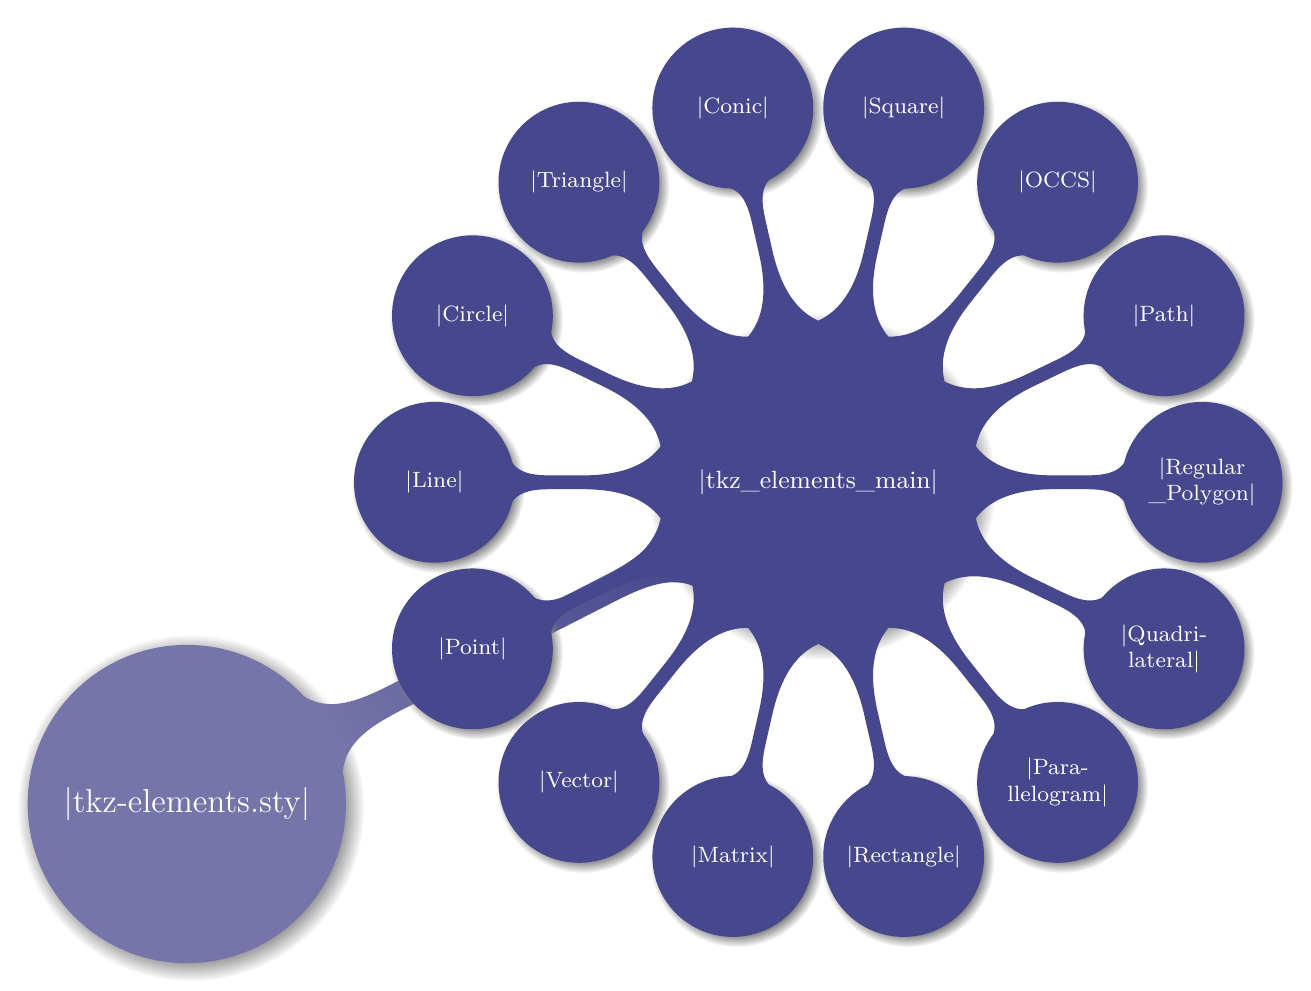
\begin{tikzpicture}[scale=.75]
\begin{scope}
\path[mindmap, concept color=MidnightBlue!60, text=white,text width=38mm,
 level 1 concept/.append style={level distance=120mm,
  sibling angle=72},
 set angles for level/.style={level 2/.append style={
 sibling angle=360/\the\tikznumberofchildren}},
 level/.append style={set angles for level=2},
 level 3 concept/.append style={level distance=20mm,
  sibling angle=20},
 L1/.style={level distance=45mm},
 L2/.style={level distance=65mm,minimum size=2cm}]

node[concept,circular drop shadow] {|tkz-elements.sty|} [clockwise from=10]

child[concept color= MidnightBlue!80,minimum size=4cm,text width=38mm,
clockwise from=27] { 
  node[concept,circular drop shadow] {|tkz\_elements\_main|} 
  [clockwise from=0]
  child[L2] { node[concept,circular drop shadow] {|Regular \_Polygon|} }
  child[L2] { node[concept,circular drop shadow] {|Quadri\-lateral|} }
  child[L2] { node[concept,circular drop shadow] {|Para\-llelogram|} }
  child[L2] { node[concept,circular drop shadow] {|Rectangle|} }
  child[L2] { node[concept,circular drop shadow] {|Matrix|} }
  child[L2] { node[concept,circular drop shadow] {|Vector|} }
  child[L2] { node[concept,circular drop shadow] {|Point|} }
  child[L2] { node[concept,circular drop shadow] {|Line|} }
  child[L2] { node[concept,circular drop shadow] {|Circle|} }
  child[L2] { node[concept,circular drop shadow] {|Triangle|} }
  child[L2] { node[concept,circular drop shadow] {|Conic|} }
  child[L2] { node[concept,circular drop shadow] {|Square|} }
  child[L2] { node[concept,circular drop shadow] {|OCCS|} }
  child[L2] { node[concept,circular drop shadow] {|Path|} }
};
\end{scope}
\end{tikzpicture}

The current classes are :

 \tkzClass{point} (z), \tkzClass{circle} (C), \tkzClass{line} (L), \tkzClass{matrix} (M), \tkzClass{occs} (O), \tkzClass{parallelogram} (P), \tkzClass{quadrilateral} (Q), \tkzClass{rectangle} (R), \tkzClass{square} (S), \tkzClass{triangle} (T), \tkzClass{vector} (V), \tkzClass{conic} (CO),   \tkzClass{regular\_polygon} (RP) and \tkzClass{path} (PA).\\
 
  The variable in parentheses indicates the name typically assigned to the table containing objects of the corresponding class.  

If \tkzname{name} refers to a class, its definition can be found in the file \code{tkz\_elements\_name.lua}.
     
% section structure (end)



\newpage
\section{Why tkz-elements?}

The \tkzNamePack{tkz-elements} package was created to address two key challenges in geometric work with TeX. First, TeX alone lacks the numerical precision and flexibility required for complex geometric calculations. By leveraging \tkzname{Lua}, \tkzNamePack{tkz-elements} provides accurate and stable computations for operations such as intersections, projections, and transformations.

Second, the package introduces an object-oriented approach to geometry. Geometric entities—such as points, vectors, lines, circles, and conics—are modeled as structured objects with associated methods. This allows users to express geometric relationships in a more natural and readable way, similar to mathematical language.

Beyond these two core ideas, \tkzNamePack{tkz-elements} offers several additional benefits:

\begin{itemize}

 \item  Simplified computations: \tkzname{Lua}'s floating-point arithmetic and expressive syntax make geometric calculations much easier to write and understand than in pure TeX.

\item   Extensibility: Thanks to its modular design and use of classes, new geometric objects and methods can be added with minimal effort, making the package scalable and adaptable.

\item   Interoperability: Calculated points and data integrate smoothly with \TIKZ{} or other TeX drawing tools, allowing users to combine computation and visualization effectively.

 \item  Pedagogical clarity: With its structured and expressive syntax, \tkzNamePack{tkz-elements} is well-suited for educational purposes, where clarity of construction and notation is essential.
\end{itemize}

Altogether, \tkzNamePack{tkz-elements} provides a modern, object-oriented, and Lua-powered framework for geometric constructions within the TeX ecosystem.

\subsection{Calculation accuracy}
\subsubsection{Calculation accuracy in \TIKZ}
With \TIKZ,  the expression \tkzimp{|veclen(x,y)|} calculates the expression $\sqrt{x^2+y^2}$.
This calculation is achieved through a polynomial approximation, drawing inspiration from the ideas  of \tkzimp{Rouben Rostamian}.

\pgfkeys{/pgf/number format/.cd,std,precision=5} \pgfmathparse{veclen(65,72)}
\begin{mybox}{}
\begin{verbatim}
   pgfmathparse{veclen(65,72)} \pgfmathresult
\end{verbatim}
\end{mybox}

 \tkzHand $\sqrt{65^2+72^2} \approx \pmpn{\pgfmathresult} $ \tkzRBomb.

\subsubsection{Calculation accuracy in Lua}
A |luaveclen| macro can be defined as follows:

\begin{mybox}{}
\begin{verbatim}
\def\luaveclen#1#2{\directlua{tex.print(string.format(
'\percentchar.5f',math.sqrt((#1)*(#1)+(#2)*(#2))))}}
\end{verbatim}
\end{mybox}

and

\begin{mybox}
\begin{verbatim}
\luaveclen{65}{72}
\end{verbatim}
\end{mybox}

gives
\tkzHand $\sqrt{65^2+72^2} = \pmpn{\luaveclen{65}{72}} $ {\color{red}!!}

The error, though insignificant when it comes to the placement of an object on a page by a hundredth of a point, becomes problematic for the results of mathematical demonstrations. Moreover, these inaccuracies can accumulate and lead to erroneous constructions.

\vspace{.5em}
To address this lack of precision, I initially introduced the \tkzNamePack{fp}, followed by the package \tkzNamePack{xfp}. More recently, with the emergence of lua\LATEX{}, I incorporated a \tkzname{Lua} option aimed at performing calculations with \tkzname{Lua}.

This was the primary motivation behind creating the package, with the secondary goal being the introduction of object-oriented programming (OOP) and simplifying programming with Lua. The concept of OOP persuaded me to explore its various possibilities further.

At that time, I had received some Lua programming examples from {\tkzimpbf{Nicolas Kisselhoff}}, but I struggled to understand the code initially, so I dedicated time to studying Lua patiently. Eventually, I was able to develop \tkzname{\tkznameofpack}, incorporating many of his ideas that I adapted for the package.

\subsubsection{Using objects}
Subsequently, I came across an article by \tkzimp{Roberto Giacomelli}\footnote{\href{https://www.guitex.org/home/images/meeting2012/slides/presentazione_giacomell_guitmeeting_2012.pdf}{Grafica ad oggetti con LuaTEX}}  on object-oriented programming using \tkzname{Lua} and \tkzNamePack{\TIKZ} tools. This served as my second source of inspiration.   Not only did this approach enable programming to be executed step-by-step, but the introduction of objects facilitated a direct link between the code and geometry. As a result, the code became more readable, explicit, and better structured.


\subsubsection{Example: Apollonius circle (new version 2025/05/12)}
\label{ssub:example_apollonius_circle}

\begin{mybox}{Problem:}
The objective is to identify an inner tangent circle to the three exinscribed circles of a triangle.\end{mybox}


For additional information, you can consult the corresponding entry on \href{https://mathworld.wolfram.com/ApolloniusCircle.html}{MathWorld}.
This example was used as a reference to test the \tkzNamePack{tkz-euclide} package. Initially, the results obtained with basic methods and available tools lacked precision. Thanks to \tkzNamePack{tkz-elements}, more powerful and accurate tools are now available — and they are also easier to use.
The core principles of figure construction with \tkzNamePack{tkz-euclide} remain unchanged: definitions, calculations, drawings, and labels, all following a step-by-step process that mirrors classical compass-and-straightedge constructions.
This version takes advantage of the simplest construction method enabled by \tkzname{Lua}.


\begin{mybox}
\begin{verbatim}
\directlua{
 init_elements()
 z.A = point(0, 0)
 z.B = point(6, 0)
 z.C = point(0.8, 4)
 T.ABC = triangle(z.A, z.B, z.C)
 z.N = T.ABC.eulercenter
 z.S = T.ABC.spiekercenter
 T.feuerbach = T.ABC:feuerbach()
 z.Ea, z.Eb, z.Ec = T.feuerbach:get()
 T.excentral = T.ABC:excentral()
 z.Ja, z.Jb, z.Jc = T.excentral:get()
 C.JaEa = circle(z.Ja, z.Ea)
% C.ortho = circle:radius(z.S, math.sqrt(C.JaEa:power(z.S)))
 C.ortho = C.JaEa:orthogonal_from(z.S) % 2025/05/12
 z.a = C.ortho.through
 C.euler = T.ABC:euler_circle()
 C.apo = C.ortho:inversion(C.euler)
 z.O = C.apo.center
 z.xa, z.xb, z.xc = C.ortho:inversion(z.Ea, z.Eb, z.Ec)}
\end{verbatim}
\end{mybox}

Creating an object involves defining its attributes and methods — that is, its properties and the actions it can perform. Once created, the object is associated with a name (or reference) by storing it in a table. This table acts as an associative array, linking a \code{key} (the reference) to a \code{value} (the object itself). These concepts will be explored in more detail later.

For instance, suppose \code{T} is a table that associates the triangle object with the key \code{ABC}. Then \code{T.ABC} refers to another table containing the attributes of the triangle — such as its vertices, sides, or angles — each accessible via a specific key. These attributes are predefined within the package to support geometric operations.

\vspace{1em}
\begin{mybox}
\begin{verbatim}
 z.N = T.ABC.eulercenter
\end{verbatim}
\end{mybox}

\code{N} is the name of the point, \code{eulercenter} is an attribute of the triangle.
\footnote{ The center of the Euler circle, or center of the nine-point circle, is a characteristic of every triangle.}

\begin{mybox}
\begin{verbatim}
 T.excentral     = T.ABC : excentral ()
\end{verbatim}
\end{mybox}

In this context, \tkzname{excentral} is a method associated with the \tkzname{T.ABC }object. It defines the triangle formed by the centers of the exinscribed circles.


\begin{tcolorbox}[
  title=Deprecated Code,
  colframe=red!50,
  colback=red!5,
  coltitle=black,
  sharp corners,
  fonttitle=\bfseries,
  leftrule=1mm,
  rightrule=1mm,
  toprule=0.5mm,
  bottomrule=0.5mm
]
\textbf{Note:} This code has been replaced by a more elegant version.

Two lines were particularly noteworthy. The first demonstrates how the exceptional precision of \tkzname{Lua} allows a radius to be defined through a complex computation.

The radius of the radical circle is given by:
\[
\sqrt{\Pi(S,\mathcal{C}(Ja,Ea))}
\]
(the square root of the power of the point $S$ with respect to the exinscribed circle centered at |Ja| and passing through |Ea|).

\begin{mybox}{}
\begin{verbatim}
  C.ortho  = circle: radius (z.S,math.sqrt(C.JaEa: power(z.S)))
\end{verbatim}
\end{mybox}
\end{tcolorbox}

\begin{tcolorbox}[
  title=Revised Code,
  colframe=cyan!60!black,
  colback=cyan!5,
  coltitle=white,
  sharp corners,
  fonttitle=\bfseries,
  leftrule=1mm,
  rightrule=1mm,
  toprule=0.5mm,
  bottomrule=0.5mm
]
\textbf{Note:} The following code replaces the previous version with a more elegant and object-oriented approach.
The previous code demonstrated the kinds of calculations that can be performed manually. However, \tkzNamePack{tkz-elements} offers a wide range of methods associated with the various geometric objects. Among the methods related to circles is one that allows you to define a circle orthogonal to another, given a center point.

We want to obtain the circle orthogonal to the three exinscribed circles of the triangle. Its center ($S$) is the radical center of these three circles. It suffices to compute a circle orthogonal to one of them \footnote{Given a main circle and two secondary circles, a specific method exists for defining the radical circle orthogonal to all three.}, taking as center the point $S$.

The second important line performs an inversion with respect to this orthogonal circle.

\begin{mybox}{}
\begin{verbatim}
  C.ortho  = C.JaEa:orthogonal_from(z.S)
\end{verbatim}
\end{mybox}
\end{tcolorbox}

\vspace{1em}

Lastly, it's worth noting that the inversion of the Euler circle with respect to the radical circle yields the Apollonius circle.\footnote{The nine-point circle, also known as Euler's circle, is externally tangent to the three exinscribed circles. The points of tangency form the Feuerbach triangle.}

This transformation requires an object as a parameter. The method automatically detects the object type (as all objects in the package are typed) and selects the appropriate algorithm accordingly.

\begin{mybox}{}
\begin{verbatim}
  C.apo   = C.ortho : inversion (C.euler)
\end{verbatim}
\end{mybox}

Now that all relevant points have been defined, it is time to begin drawing the geometric paths. To do this, the corresponding nodes must first be created. This is precisely the role of the macro \tkzMacro{tkz-elements}{tkzGetNodes} (see Section~\ref{ssub:points_transfer}).

The subsequent section exclusively deals with drawings, and is managed by \tkzNamePack{tkz-euclide}.

\begin{verbatim}
\begin{tikzpicture}
   \tkzGetNodes
   \tkzFillCircles[green!30](O,xa)
   \tkzFillCircles[teal!30](Ja,Ea Jb,Eb Jc,Ec)
   \tkzFillCircles[lightgray](S,a)
   \tkzFillCircles[green!30](N,Ea)
   \tkzDrawPoints(xa,xb,xc)
   \tkzDrawCircles(Ja,Ea Jb,Eb Jc,Ec S,a O,xa N,Ea)
   \tkzClipCircle(O,xa)
   \tkzDrawLines[add=3 and 3](A,B A,C B,C)
   \tkzDrawPoints(O,A,B,C,S,Ea,Eb,Ec,N)
   \tkzDrawSegments[dashed](S,xa S,xb S,xc)
   \tkzLabelPoints(O,N,A,B)
   \tkzLabelPoints[right](S,C)
\end{tikzpicture}
\end{verbatim}

\vspace{1em}
\directlua{
 init_elements()
 z.A = point(0, 0)
 z.B = point(6, 0)
 z.C = point(0.8, 4)
 T.ABC = triangle(z.A, z.B, z.C)
 z.N = T.ABC.eulercenter
 z.S = T.ABC.spiekercenter
 T.feuerbach = T.ABC:feuerbach()
 z.Ea, z.Eb, z.Ec = T.feuerbach:get()
 T.excentral = T.ABC:excentral()
 z.Ja, z.Jb, z.Jc = T.excentral:get()
 C.JaEa = circle(z.Ja, z.Ea)
 C.ortho = C.JaEa:orthogonal_from(z.S)
 z.a = C.ortho.through
 C.euler = T.ABC:euler_circle()
 C.apo = C.ortho:inversion(C.euler)
 z.O = C.apo.center
 z.xa, z.xb, z.xc = C.ortho:inversion(z.Ea, z.Eb, z.Ec)
}
\begin{minipage}{\textwidth}

\begin{center}
\begin{tikzpicture}[ scale  = .4]
   \tkzGetNodes
   \tkzFillCircles[green!30](O,xa)
   \tkzFillCircles[teal!30](Ja,Ea Jb,Eb Jc,Ec)
   \tkzFillCircles[lightgray](S,a)
   \tkzFillCircles[green!30](N,Ea)
   \tkzDrawPoints(xa,xb,xc)
   \tkzDrawCircles(Ja,Ea Jb,Eb Jc,Ec S,a O,xa N,Ea)
   \tkzClipCircle(O,xa)
   \tkzDrawLines[add=3 and 3](A,B A,C B,C)
   \tkzDrawPoints(O,A,B,C,S,Ea,Eb,Ec,N)
   \tkzDrawSegments[dashed](S,xa S,xb S,xc)
   \tkzLabelPoints(O,N,A,B)
   \tkzLabelPoints[right](S,C)
\end{tikzpicture}
\end{center}
\end{minipage}
\endinput
\newpage
\section{Presentation}
\subsection{Geometric Construction Philosophy}
\tkzNamePack{tkz-elements} is built around the principles of classical Euclidean geometry, emphasizing constructions achievable with an unmarked straightedge and a compass. The library favors a declarative and geometric approach over algebraic or numeric definitions.

This philosophy means that all geometric objects — points, lines, circles, triangles, and so on — are primarily defined by other points. Explicit numerical values such as coordinates, distances, or angles are deliberately avoided unless they are essential to the construction. This is in line with a traditional ruler-and-compass mindset, where geometric reasoning emerges from visual configurations and not from numbers.

For example:
\begin{itemize}
  \item A circle is defined by its center and a point on the circumference,
  \item A perpendicular bisector is constructed using midpoint and symmetry,
  \item An angle is inferred from three points rather than given as a numeric value.
\end{itemize}

This design decision also explains why constructors based on scalar values, such as OCCS (One Center and a Scalar), are not part of the default interface. Their use would introduce numerical dependency at odds with the intended geometric abstraction.

\bigskip
While \tkzNamePack{tkz-elements} promotes a high-level, point-based approach to geometry, it relies internally on \textbf{Lua} for performing all necessary calculations. Lua is not exposed to the user as a scripting tool, but rather serves as a powerful computational engine that enables precise and robust geometric operations behind the scenes.

This separation of concerns allows users to focus entirely on geometric constructions while benefiting from Lua’s computational precision and performance. In the next section, we will explain how Lua integrates with \LaTeX\ in the context of this package — not as a programming layer, but as an invisible partner enabling advanced constructions.


\subsection{With Lua}
The primary purpose of \tkzNamePack{tkz-elements} is to perform geometric computations and define points using \tkzname{Lua}. You can think of it as a computational kernel that can be used by either \tkzNamePack{tkz-euclide} or directly with \tkzNamePack{\TIKZ}.

\tkzname{Lua} code can be executed in two ways: directly, using the \tkzMacro{lualatex}{directlua} primitive, or within a \tkzEnv{tkz-elements}{tkzelements} environment based on the \tkzNamePack{luacode} package (which must be loaded separately).
When using \tkzMacro{lualatex}{directlua}, especially in complex documents, you can reset internal data structures — such as coordinate tables and scaling factors — using the \tkzFct{package}{init\_elements()} function.

\begin{minipage}[t]{.52\textwidth}\vspace{0pt}%
   The key points are:
   \begin{itemize}
      \item The source file must be \tkzRHand\ {\color{red}\uline{ \color{black}UTF-8}}  encoded.
      \item Compilation must be done with  \tkzRHand\ {\color{red}\uline{ \color{black}lua\LATEX{}}}.
      \item You need to load \tkzNamePack{tkz-euclide} and \code{tkz-elements}.
      \item All definitions and calculations are carried out in an \tkzClass{occs} (orthonormal cartesian coordinate system,) using Lua either via the macro \tkzMacro{lualatex}{directlua} or within the  \tkzEnv{tkz-elements}{tkzelements} environment.
   \end{itemize}

On the right, you will find a minimal template.

The code is divided into two main parts:  the Lua code (executed using \tkzMacro{lualatex}{directlua} or placed inside a \tkzEnv{tkz-elements}{tkzelements} environment), and the  \tkzEnv{tikz}{tikzpicture} environment, where drawing commands — typically from \tkzNamePack{tkz-euclide} — are issued.

When using \tkzNamePack{tkz-euclide}, the mini option is recommended to load only the macros needed for drawing.
Within the \tkzname{Lua} section, it is best practice to systematically call the \tkzFct{package}{init\_elements()} function. This function resets internal tables.
Important: From this point on, all scaling operations must be avoided in the \tkzname{Lua} code.

\vspace*{4.1 cm}%
\end{minipage}\hspace*{\fill}
\begin{minipage}[t]{.45\textwidth}\vspace{0pt}%
\begin{mybox}
\begin{verbatim}
% !TEX TS-program = lualatex
% Created by Alain Matthes
\documentclass{standalone}
\usepackage[mini]{tkz-euclide}
% or simply TikZ
\usepackage{tkz-elements}
begin{document}

\directlua{
init_elements()
% definition of some points
z.A = point(   ,   )
z.B = point(   ,   )
% or
z.A = point:new(   ,   )
z.B = point:new(   ,   )

 ...code...
}

\begin{tikzpicture}
% points transfer to Nodes
% from Lua to tikz (tkz-euclide)
\tkzGetNodes

\end{tikzpicture}
\end{document}
\end{verbatim}
\end{mybox}
\end{minipage}

\subsection{The main process}

\tikzset{concept/.append style={fill={none}}}
\tikzset{root concept/.style=   {minimum size=3cm,text width=2.8cm}}%
\tikzset{level 1 concept/.append style={minimum size=4cm, font=\large, text width=3cm}}%
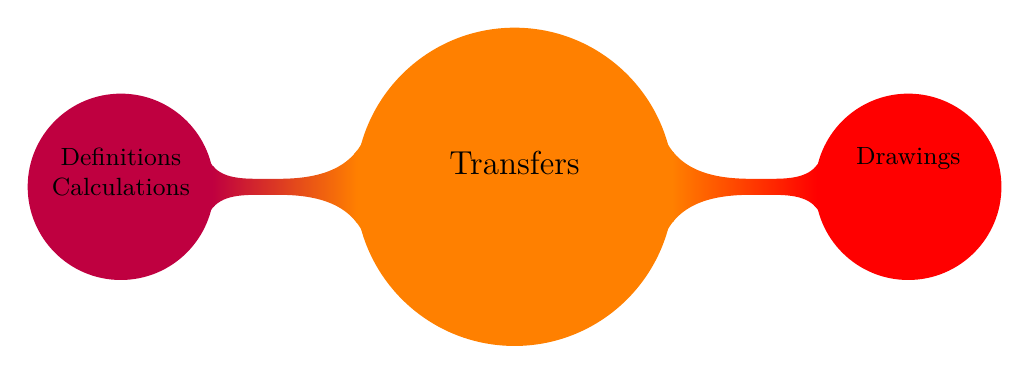
\begin{tikzpicture}
  \path[mindmap,concept color=orange,text=black]
    node[concept] {Transfers\\\textcolor{orange}{ \textbackslash{tkzGetNodes}}}
    child[concept color=red,grow=right] {
      node[concept] {Drawings\\\textcolor{red}{tkz-euclide}\\\textcolor{red}{\TIKZ}} }
    child[concept color=purple,grow=left] {
    node[concept] {Definitions\\Calculations\\\textcolor{purple}{tkz-elements}} };
\end{tikzpicture}

After obtaining all the necessary points for the drawing, they must be transformed into \tkzname{nodes} so that \tkzNamePack{\TIKZ} or \tkzNamePack{tkz-euclide} can render the figure. This is accomplished using the macro \tkzMacro{tkz-elements}{tkzGetNodes}. This macro iterates through  all the elements of the table \tkzname{z} using the key (which is essentially the name of the point) and retrieves the associated values, namely the coordinates of the point (node).

\subsection{Complete example: Pappus circle}
\label{sub:the_figure_pappus_circle}


\subsubsection{The figure}

\directlua{
z.A = point(0, 0)
z.B = point(10, 0)
L.AB = line(z.A, z.B)
z.C = L.AB:gold_ratio()
L.AC = line(z.A, z.C)
L.CB = line(z.C, z.B)
L.AB = line(z.A, z.B)
z.O_0 = L.AB.mid
z.O_1 = L.AC.mid
z.O_2 = L.CB.mid
C.AB = circle(z.O_0, z.B)
C.AC = circle(z.O_1, z.C)
C.CB = circle(z.O_2, z.B)
z.P = C.CB.north
z.Q = C.AC.north
z.O = C.AB.south
z.c = z.C:north(2)
C.PC = circle(z.P, z.C)
C.QA = circle(z.Q, z.A)
z.P_0 = intersection(C.PC, C.AB)
z.P_1 = intersection(C.PC, C.AC)
_, z.P_2 = intersection(C.QA, C.CB)
T.P = triangle(z.P_0, z.P_1, z.P_2)
z.O_3 = T.P.circumcenter
}

\begin{center}
\begin{tikzpicture}[scale = .75]
 \tkzGetNodes
 \tkzDrawCircle[black,fill=yellow!20,opacity=.4](O_0,B)
 \tkzDrawCircles[teal,fill=teal!40,opacity=.6](O_1,C O_2,B)
 \tkzDrawCircle[purple,fill=purple!20,opacity=.4](O_3,P_0)
 \tkzDrawArc[cyan,delta=10](Q,A)(P_0)
 \tkzDrawArc[cyan,delta=10](P,P_0)(B)
 \tkzDrawArc[cyan,delta=10](O,B)(A)
 \tkzDrawPoints(A,B,C,O_0,O_1,O_2,P,Q,P_0,P_0,P_1,P_2,O)
 \tkzLabelPoints(A,B,C,O_0,O_1,O_2,P,Q,P_0,P_0,P_1,P_2,O)
\end{tikzpicture}
\end{center}

\subsubsection{The code}
\label{ssub:the_code}

\begin{verbatim}
% !TEX TS-program = lualatex
\documentclass{article}
\usepackage[mini]{tkz-euclide} % mini = only tracing function
\usepackage{tkz-elements}
\begin{document}

\directlua{
  init_elements()  % Clear tables
  z.A = point(0, 0)
  z.B = point(10, 0)  %  creation of two fixed points $A$ and $B$
  L.AB = line(z.A, z.B)
  z.C = L.AB:gold_ratio()       %  use of a method linked to “line”
  z.O_0 = line(z.A, z.B).mid % midpoint of segment with an attribute of “line”
  z.O_1 = line(z.A, z.C).mid %  objects are not stored and cannot be reused.
  z.O_2 = line(z.C, z.B).mid
  C.AB = circle(z.O_0, z.B)  %  new object “circle” stored and reused
  C.AC = circle(z.O_1, z.C)
  C.CB = circle(z.O_2, z.B)
  z.P = C.CB.north            %  “north” atrributes of a circle
  z.Q = C.AC.north
  z.O = C.AB.south
  z.c = z.C:north(2)   %“north” method of a point (needs a parameter)
  C.PC = circle(z.P, z.C)
  C.QA = circle(z.Q, z.A)
  z.P_0 = intersection(C.PC,C.AB)   %  search for intersections of two circles.
  z.P_1 = intersection(C.PC,C.AC)   %   idem
  _,z.P_2 = intersection(C.QA,C.CB)   %  idem
  T.P = triangle(z.P_0, z.P_1, z.P_2)
  z.O_3 = T.P.circumcenter  % circumcenter attribute of “triangle”
}
\end{verbatim}

\begin{verbatim}
\begin{tikzpicture}
  \tkzGetNodes
  \tkzDrawCircle[black,fill=yellow!20,opacity=.4](O_0,B)
  \tkzDrawCircles[teal,fill=teal!40,opacity=.6](O_1,C O_2,B)
  \tkzDrawCircle[purple,fill=purple!20,opacity=.4](O_3,P_0)
  \tkzDrawArc[cyan,delta=10](Q,A)(P_0)
  \tkzDrawArc[cyan,delta=10](P,P_0)(B)
  \tkzDrawArc[cyan,delta=10](O,B)(A)
  \tkzDrawPoints(A,B,C,O_0,O_1,O_2,P,Q,P_0,P_0,P_1,P_2,O)
  \tkzLabelPoints(A,B,C,O_0,O_1,O_2,P,Q,P_0,P_0,P_1,P_2,O)
\end{tikzpicture}
\end{document}
\end{verbatim}

\subsection{Another example with comments: South Pole}
Here's another example with comments

\begin{verbatim}
% !TEX TS-program = lualatex
\documentclass{standalone}
\usepackage[mini]{tkz-euclide}
\usepackage{tkz-elements}
\begin{document}
\directlua{
 init_elements()                     % Clear tables
 z.A = point(2, 4)
 z.B = point(0, 0)                   % three fixed points are used
 z.C = point(8, 0)                   %
 T.ABC = triangle(z.A, z.B, z.C)     % we create a new triangle object
 C.ins = T.ABC:in_circle()           % we get the incircle of this triangle
 z.I = C.ins.center                  % center is an attribute of the circle
 z.T = C.ins.through                 % through is also an attribute
 z.I, z.T = C.ins:get()              % get() is a shortcut
 C.cir = T.ABC:circum_circle()       % we get the  circumscribed circle
 z.W = C.cir.center                  % we get the center of this circle
 z.O = C.cir.south                   % now we get the south pole of this circle
 L.AO = line(z.A, z.O)               % we create an object "line"
 L.BC = T.ABC.bc                     % we get the line (BC)
 z.I_A = intersection(L.AO, L.BC)    % we search the intersection of the last lines
}
\end{verbatim}

\directlua{
 init_elements()
 z.A = point(2, 4)
 z.B = point(0, 0)
 z.C = point(8, 0)
 T.ABC = triangle(z.A, z.B, z.C)
 C.ins = T.ABC:in_circle()
 z.I = C.ins.center
 z.T = C.ins.through
 C.cir = T.ABC:circum_circle()
 z.W = C.cir.center
 z.O = C.cir.south
 L.AO = line(z.A, z.O)
 L.BC = T.ABC.bc
 z.I_A = intersection(L.AO, L.BC)
}

\begin{center}
  \begin{tikzpicture}[ scale= 1.2]
  \tkzGetNodes
  \tkzDrawCircles(W,A I,T)
  \tkzDrawArc(O,C)(B)
  \tkzDrawPolygon(A,B,C)
  \tkzDrawSegments[new](A,O B,O C,O)
  \tkzDrawLine(B,I)
  \tkzDrawPoints(A,B,C,I,I_A,W,O)
  \tkzFillAngles[green!20,opacity=.3](A,O,B A,C,B)
  \tkzFillAngles[teal!20,opacity=.3](O,B,C B,C,O B,A,O O,A,C)
  \tkzLabelPoints(I,I_A,W,B,C,O)
  \tkzLabelPoints[above](A)
  \end{tikzpicture}
\end{center}

\vspace{12pt}
Here's the \tkzEnv{tikz}{tikzpicture} environment to obtain the drawing:
\begin{verbatim}
\begin{tikzpicture}
\tkzGetNodes
\tkzDrawCircles(W,A I,T)
\tkzDrawArc(O,C)(B)
\tkzDrawPolygon(A,B,C)
\tkzDrawSegments[new](A,O B,O C,O)
\tkzDrawLine(B,I)
\tkzDrawPoints(A,B,C,I,I_A,W,O)
\tkzFillAngles[green!20,opacity=.3](A,O,B A,C,B)
\tkzFillAngles[teal!20,opacity=.3](O,B,C B,C,O B,A,O O,A,C)
\tkzLabelPoints(I,I_A,W,B,C,O)
\tkzLabelPoints[above](A)
\end{tikzpicture}
\end{verbatim}
\endinput
\newpage

\section{Writing Convention, best practices and common mistakes} % (fold)
\label{sec:writing_convention}
\subsection{Assigning a Name to an Object} % (fold)
\label{sub:assigning_a_name_to_an_object}

\textbf{Note:} Certain variables such as \tkzname{z}, \tkzname{L}, \tkzname{T}, etc. are reserved for storing geometric objects.
Reassigning one of them (e.g., \tkzname{L = 4}) will overwrite its content and disrupt the system.

Points are a special case: they must be stored in the table \tkzname{z}.
For all other geometric objects, it is strongly recommended to follow the predefined variable names.
Avoid mixing naming conventions or inventing your own identifiers, as this may lead to unpredictable behavior.

\vspace{1em}
\tkzRHand{\textcolor{red}{Warning}}: Do not reuse names such as \texttt{point}, \texttt{line}, \texttt{circle}, \texttt{path}, \texttt{triangle}, etc., as variable names.
These identifiers are reserved internally by \tkzNamePack{tkz-elements} to represent object constructors.

\vspace{1em}
Below is the list of reserved classes and the default variable names associated with them:
\label{list of reserved classes}

\vspace{1em}
\textcolor{red}{\directlua{
local variables = { "C", "CO", "L", "M", "O", "P", "PA", "z", "Q", "R", "RP", "S", "T", "V"}
local modules = { "circle",  "conic",  "line", "matrix", "occs", "parallelogram", "path",  "point", "quadrilateral", "rectangle", "regular\\_polygon", "square",  "triangle", "vector"}
  for i = 1, utils.table_getn(modules) do
    local class = modules[i]
    local var   = variables[i]
    tex.sprint( class.. "  -->  ".. var.."\\\\")
  end
} }

\subsection{Best practices} % (fold)
\label{sub:best_practices}

It is preferable to use methods—or better yet, object attributes—rather than standalone functions.

For example, to determine the midpoint of a segment $AB$, iit was previously possible to write: |z.m = midpoint (z.A,z.B)|.  This is now considered incorrect: you must use |z.m = tkz.midpoint (z.A,z.B)|.

However, the recommended approach is to define the segment first with: |L.AB = line(z.A, z.B)|, and then use the attribute: |z.m = line(z.A, z.B).mid|. If you don't reuse the line, a one-liner like |z.m = line(z.A, z.B).mid| is acceptable.

\vspace{12pt}
Similarly, it may have been tempting to write |L.bi = bisector(z.A, z.B, z.C)| to obtain the angle bisector at vertex $A$. As in the previous example, this is no longer valid. You must now use |L.bi = tkz.bisector(z.A, z.B, z.C)|, as all standalone functions have been grouped under the |tkz| module.

A better practice is to define the triangle $ABC$ using:  |T.ABC = triangle(z.A, z.B, z.C)| and then access the bisector via: |L.bi = T.ABC:bisector(z.A)| or directly: |L.bi = triangle(z.A, z.B, z.C):bisector(z.A)|.

% subsection best_practices (end)

\subsection{Common mistakes and best practices}

\vspace{1em}
\tkzRHand{\textcolor{red}{Second Warning}}: Let's examine the consequences of incorrect assignments. The following example is very simple: we define two points, the line passing through them, and a line orthogonal to the first at one of the points. To define these objects, we use two tables (or classes): \tkzname{z} and \tkzname{L}.

Here is the correct code:
\begin{tkzexample}[latex=.5\textwidth]
\directlua{
  z.A = point(1, 2)
  z.B = point(3, -1)
  L.AB = line(z.A, z.B)
  -- blunders
  L.ortho = L.AB:ortho_from(z.B)
  z.C = L.ortho.pb
}
\begin{tikzpicture}[scale = .75]
  \tkzGetNodes
  \tkzDrawLines(A,B B,C)
  \tkzDrawPoints(A,B)
\end{tikzpicture}
\end{tkzexample}

\begin{itemize}
  \item \textbf{First blunder:} \tkzname{z = nil} or \tkzname{z = 4}. You've reassigned the \tkzname{z} variable. It no longer refers to a table, but to a number. Its type has changed, and the system can no longer access the points.
  \item \tkzname{z.A = 4} is equally problematic: you’ve overwritten point $A$. If your intention is to remove point $A$, then use \tkzname{z.A = nil} instead.
  \item \tkzname{L = 4}. This might seem convenient to store a length, but doing so will erase the entire table of lines.
  \item \tkzname{L.ortho = ortho}. A more subtle mistake: if \tkzname{ortho} is not defined, you lose your line. If it is defined but of the wrong type, an error will occur.
  \item For objects other than points, incorrect assignments at the end of the process may not affect the figure. It is possible to clean up tables before plotting. However, the \tkzname{z} table must not be altered. Only points not used for plotting should be deleted.
\end{itemize}

These precautions help ensure consistency in the system and prevent unpredictable behavior.

\vspace{1em}
We’ll now explain how to assign variable names for each type of object.

\subsection{Assigning a Name to a Point} % (fold)
\label{sub:assigning_a_name_to_a_point}

At present, points must be stored in the table \tkzname{z} if you intend to use them later in \tkzNamePack{\TIKZ} or \tkzNamePack{tkz-euclide}.

In \tkzNamePack{tkz-elements}, points must follow the \tkzname{z.name} convention, where name is the label of the corresponding node.

Special attention is needed for certain naming cases:


\begin{enumerate}

\item \emph{Primes (or double prime) can be problematic.}\\

If a point’s name ends in |p| (like Bp),  then when passing into \tkzNamePack{tkz-euclide}, this is interpreted during transfer to \tkzNamePack{tkz-euclide} via \tkzMacro{tkz-elements}{tkzGetNodes}; \index{prime} as a prime, and |p| will be converted into |'|, giving B' in the \tkzNamePack{\TIKZ} output.

   \item  \emph{For clarity or complex names, you may use intermediate variables.}\\

 For example, if you want to define a point named \tkzname{euler}, you could write:

 \begin{mybox}
 |local euler = point(...)| or |z.euler = point(...)|
  and at the end |z.E = euler| or |z.E = z.euler|
 \end{mybox}

  In this case, the point will be labeled E in the drawing, but internally it remains clear in code.
  Alternatively, you can keep the name euler in Lua and alias it for display with:

\begin{mybox}
|pgfnodealias{E}{euler}| in \TIKZ{}.
\end{mybox}

\end{enumerate}


Examples of valid naming:
\begin{mybox}
\begin{itemize}
   \item |z.A = point(1,2)|
   \item |z.Bp = point(3,4)|  --> this gives |B'| in the \tkzEnv{tikz}{tikzpicture}
   \item |z.H_a = T.ABC:altitude ()| --> this gives |H_a| in the \tkzEnv{tikz}{tikzpicture} code and $H_a$ in math display.

   \item |z.euler = T.ABC.eulercenter|
\end{itemize}
\end{mybox}

In \tkzname{Lua}, |z.A| is a "sugar syntax" for |z["A"]| and |z.A = nil| deletes point $A$.

% subsection assigning_a_name_to_a_point (end)

\subsection{Assigning a Name to Other Objects} % (fold)
\label{sub:assigning_a_name_to_other_objects}
For all geometric objects other than points, you are free to choose names. However, adopting consistent conventions greatly improves code readability and maintainability. To be more precise, each Lua code block is usually preceded by the call to the function \tkzFct{package}{init\_elements()}, whose role is to clear and reset the various tables (such as \tkzname{L}, \tkzname{C}, etc.).
If you choose to use custom variable names or structures, you are free to do so — but in that case, you are responsible for managing and cleaning your variables and tables manually to avoid conflicts or unintended behavior.

In this documentation, the following naming strategy is used:


Objects are stored in dedicated tables, each associated with a specific class.
These tables are represented by variables such as:
\begin{itemize}

\item \tkzname{L} for lines and segments
\item \tkzname{C} for circles
\item \tkzname{T} for triangles
\item  \tkzname{CO} for conics (including ellipses, hyperbolas, and parabolas)

\item  etc. See the list of reserved words [\ref{list of reserved classes}]
\end{itemize}

Here are some examples of naming conventions used:

\begin{itemize}
  \item Lines (L):\\
  The name reflects the two points defining the line.

   Example: |L.AB = line(z.A, z.B)| -- line through A and B

\item Circle (C)\\
You can name a circle based on its defining points or its purpose.
Examples:
\begin{itemize}
 \item C.AB       --> Circle centered at A, passing through B
 \item C.euler    --> Euler circle
 \item C.external --> External circle
\end{itemize}

\item Triangles (T)\\
Use vertex labels, or descriptive names when appropriate. Examples:

\begin{itemize}
  \item T.ABC         --> Triangle with vertices A, B, C
  \item T.feuerbach   --> Feuerbach triangle

\end{itemize}



\item Conics (CO)\\
The table CO can store various conics; use meaningful keys to indicate type and role.


\end{itemize}

Note: \emph{While you may choose other variable names or formats, following these conventions ensures that your code remains clear and easy to follow, especially when working with more complex figures.}

% subsection assigning_a_name_to_other_objects(end)

\subsection{Writing conventions for attributes, methods.} % (fold)
\label{sub:writing_conventions_for_attributes_methods_and_functions}

You must follow standard Lua conventions when accessing attributes or invoking methods:

\begin{itemize}
  \item \textbf{Attributes} are accessed using the dot notation: \verb|object.attribute|.
    \begin{itemize}
      \item For example, to access the coordinates of point \verb|A|, use \verb|z.A.re| for the abscissa and \verb|z.A.im| for the ordinate.
      \item To get the type of the object, write \verb|z.A.type|.
      \item To retrieve the south pole of the circle \verb|C.OA|, write \verb|C.OA.south|.
    \end{itemize}

  \item \textbf{Methods} are invoked using the colon notation: \verb|object:method()|.
    \begin{itemize}
      \item For example, to compute the incircle of triangle \verb|ABC|, use: \verb|C.incircle = T.ABC:in_circle()|.
      \item If a method requires a parameter, include it in parentheses. For instance, to compute the distance from point \verb|C| to the line \verb|(AB)|: \verb|d = L.AB:distance(z.C)|.
    \end{itemize}

  \item \textbf{Discarding results}: If a function returns multiple values and you only need one, use \verb|_| to ignore the rest.
    \begin{itemize}
      \item For example, to retrieve only the second point of intersection between a line and a circle: \verb|_, z.J = intersection(L.AB, C.OC)|.
    \end{itemize}
\end{itemize}

% subsection assigning_a_name_to_an_object (end)


\subsection{Miscellaneous} % (fold)
\label{sub:miscellanous}
\begin{itemize}
  \item \textbf{Units and coordinates:} As in \tkzNamePack{tkz-euclide}, the default unit is the centimeter. All points are placed in an orthonormal Cartesian coordinate system.

  \item \textbf{Numerical variables:} Real numbers follow the standard Lua conventions for notation.

  \item \textbf{Complex numbers:} Similar to real numbers, but you must define them using the point constructor. For example:
  \begin{verbatim}
  za = point(1, 2)
  \end{verbatim}
  This corresponds mathematically to \(1 + 2i\). You can print the complex number using:
  \begin{verbatim}
  tex.print(tostring(za))
  \end{verbatim}

  \item \textbf{Boolean values:}
  \begin{itemize}
    \item In Lua: \verb|bool = true| or \verb|bool = false|
    \item You can use the following \tkzname{Lua} code:
    \begin{verbatim}
    if bool == true then ... else ... end
    \end{verbatim}
    \item In LaTeX, after loading the \tkzNamePack{ifthen} package, you can write:
    \begin{verbatim}
    \ifthenelse{\equal{\tkzUseLua{bool}}{true}}{<true code>}{<false code>}
    \end{verbatim}
  \end{itemize}

  \item \textbf{Strings:}
  \begin{itemize}
    \item Example in Lua: \verb|st = "Euler's formula"|
    \item In LaTeX: \verb|\tkzUseLua{st}| will display \texttt{Euler's formula}
  \end{itemize}
\end{itemize}

% subsection miscellanous (end)
% section writing_convention (end)
\endinput
\section{Work organization}
\label{sec:work_organization}


Here is a sample organization for working with \tkzNamePack{tkz-euclide} and \tkzEngine{lua\LATEX}.

\begin{itemize}
  \item \textbf{Compilation:} Add the line:
  \begin{verbatim}
  % !TEX TS-program = lualatex
  \end{verbatim}
  to ensure that your document compiles with \tkzEngine{lua\LATEX}.

  \item \textbf{Document Class:} The \texttt{standalone} class is recommended when the goal is simply to create a figure, as it avoids unnecessary overhead.

  \item \textbf{Package Loading:} You can load \tkzNamePack{tkz-euclide} in two ways:
  \begin{itemize}
    \item \tkzcname{usepackage\{tkz-euclide\} }gives you full access to the entire package.
    \item The recommended method is to use the \tkzPopt{tkz-euclide}{mini} option, which loads only the necessary modules for drawing. You still retain the ability to draw with \TIKZ{} if desired.
  \end{itemize}

  \item \textbf{Conditionals:} The package \tkzNamePack{ifthen} is useful when you need to evaluate Boolean conditions within your document.

  \item \textbf{Lua Code Organization:} While you can embed Lua code directly with \verb|\directlua|, externalizing the code offers several advantages:
  \begin{itemize}
    \item Better syntax highlighting and code presentation in editors that support \tkzname{Lua} and \LATEX{}.
    \item Simplified commenting: \tkzname{Lua} uses \verb|--|, while \LATEX{} uses \verb|%|. Keeping Lua in a separate file avoids confusion.
    \item Reusability: external code files can be reused across multiple documents or figures.
  \end{itemize}
\end{itemize}

For simplicity, this documentation uses embedded Lua code in most cases. However, in some examples, external files are used to show you how it's done.


\vspace{12pt}
\begin{minipage}{.55\textwidth}
\begin{verbatim}
% !TEX TS-program = lualatex
% Created by Alain Matthes on 2024-01-09.
\documentclass[margin = 12pt]{standalone}
\usepackage[mini]{tkz-euclide}
\usepackage{tkz-elements,ifthen}

\begin{document}
\directlua{
 init_elements() % Clear tables
 dofile ("lua/sangaku.lua") % Load the lua code
}
\begin{tikzpicture}[ scale = .75]
 \tkzGetNodes
 \tkzDrawCircle(I,F)
 \tkzFillPolygon[color = purple](A,C,D)
 \tkzFillPolygon[color = blue!50!black](A,B,C)
 \tkzFillCircle[color = orange](I,F)
\end{tikzpicture}
\end{document}
\end{verbatim}
\end{minipage}
\begin{minipage}{.45\textwidth}
\directlua{
 init_elements()
 dofile ("lua/sangaku.lua")
}

\begin{center}
\begin{tikzpicture}[ scale = .75]
  \tkzGetNodes
  \tkzDrawCircle(I,F)
  \tkzFillPolygon[color = purple](A,C,D)
  \tkzFillPolygon[color = blue!50!black](A,B,C)
  \tkzFillCircle[color = orange](I,F)
\end{tikzpicture}
\end{center}
\end{minipage}

\vspace{12pt}
And here is the code for the \tkzname{Lua} part: the file |ex_sangaku.lua|

\vspace{1em}
\begin{minipage}{.5\textwidth}
\begin{mybox}
\begin{verbatim}
 z.A = point(0, 0)
 z.B = point(8, 0)
 L.AB = line(z.A, z.B)
 S.AB = L.AB:square()
 _, _, z.C, z.D = S.AB:get()
 z.F = S.ac:projection(z.B)
 L.BF = line(z.B, z.F)
 T.ABC = triangle(z.A, z.B, z.C)
 L.bi = T.ABC:bisector(2)
 z.c = L.bi.pb
 L.Cc = line(z.C, z.c)
 z.I = intersection(L.Cc, L.BF)
\end{verbatim}
\end{mybox}
\end{minipage}


\subsection{Scaling Policy Update}

In previous versions, it was recommended to apply scaling within the Lua part of the code. However, this guidance has now changed.

Since all geometric computations are handled in \tkzname{Lua}, applying scaling in \TIKZ{} no longer presents any issues. On the contrary, performing scaling in \tkzname{Lua} has led to several complications—particularly with the recent implementation of conic-related functions, which involve numerous distance calculations using real numbers.

These challenges prompted a review of several functions, during which some bugs related to Lua-side scaling were identified and resolved.

\medskip
\noindent
\textbf{\textcolor{red}{New Recommendation:}} From now on, scaling should be applied exclusively in the \TIKZ{} part. The \tkzname{Lua} code should operate in an unscaled, consistent coordinate system to ensure the reliability of all geometric computations.

The following documentation uses only scaling in the \tkzEnv{tikz}{tikzpicture} environment.
\endinput
\newpage\section{Coordinates}

This section outlines the various coordinate systems available to users. Given the removal of scaling operations from the \tkzname{Lua} layer, such clarification seems more necessary than ever.

\subsection{Common Use of Coordinates}
As with \tkzNamePack{tkz-euclide}, \tkzNamePack{tkz-elements} is based on a two-dimensional orthonormal Cartesian coordinate system, using centimeters as the default unit.

It would be inconsistent to use what we will see  as an \emph{occs} (orthogonal coordinate coordinate system) in a context focused on Euclidean geometry.

Moreover, the concept of a point in \tkzNamePack{tkz-elements} is tied to the affix of a complex number. To maintain code clarity and consistency, the option to modify units within Lua has been deliberately omitted.

\medskip
\noindent
\textbf{Conclusion:} For any figure created with \tkzNamePack{tkz-elements}, all points are placed within a 2D orthonormal system using centimeters.

   \begin{tikzpicture}
   \pgfkeys{/pgf/number format/.cd,std,precision=2}
   \let\pmpn\pgfmathprintnumber
   \tkzDefPoints{2/3/M,0/0/O,2/0/A,0/3/B}
   \tkzLabelPoints(O)
   \tkzLabelPoint[right](M){$M: z_M = 2 + 3i$}
   \tkzDrawPoints(M,O)
   \tkzPointShowCoord(M)
   \tkzLabelPoint[below,teal](A){$2$}
   \tkzLabelPoint[left,teal](B){$3$}
   \tkzDrawSegments[->,add = 0 and 0.25](O,B O,A)
   \begin{scope}[every annotation/.style={fill=lightgray!15,anchor = east}]
   \node [annotation,font =\small,text width=6cm] at (current bounding box.west) {
Coordinates of $M$
   \begin{mybox}{}
   \code{ z.A = point(2, 3)}
   \end{mybox}
       };
   \end{scope}
   \end{tikzpicture}

\subsection{Use of barycentric coordinates.}

A barycentric coordinate system describes the position of a point relative to a reference triangle. Any point in the plane can be expressed with barycentric coordinates, which are defined up to a scalar multiple (homothety). Alternatively, they may be normalized so their sum equals 1.

Barycentric coordinates are particularly useful in triangle geometry, especially when analyzing properties invariant under affine transformations—those not dependent on angles.

Consider a triangle $ABC$. One can define key points like the centroid and orthocenter using barycentric coordinates.

\paragraph{About the Orthocenter.}
Computing barycentric coordinates for the orthocenter requires knowledge of the triangle's angles. These are stored as attributes in the table \texttt{T.ABC}:
\begin{itemize}
  \item \texttt{T.ABC.alpha} — angle $\widehat{A}$ at vertex $A$
  \item \texttt{T.ABC.beta}  — angle $\widehat{B}$ at vertex $B$
  \item \texttt{T.ABC.gamma} — angle $\widehat{C}$ at vertex $C$
\end{itemize}

See  [\ref{ssub:_triangle_barycentric_ka_kb_kc}]

\paragraph{Retrieving Barycentric Coordinates.}
It is possible to compute the barycentric coordinates of a given point with respect to a triangle. The returned values are automatically normalized. See Section~[\ref{ssub:_triangle_barycentric__coordinates_pt}] for usage.


\begin{minipage}{.5\textwidth}
\directlua{
z.A = point(0, 0)
z.B = point(3, 1)
z.C = point(1, 3)
T.ABC = triangle(z.A, z.B, z.C)
z.G = T.ABC:barycentric(1,1,1)
z.H = T.ABC:barycentric(math.tan(T.ABC.alpha),
                        math.tan(T.ABC.beta),
                        math.tan(T.ABC.gamma))}
\begin{tikzpicture}
\tkzGetNodes
\tkzDrawPolygon(A,B,C)
\tkzDrawPoints(A,B,C,G,H)
\tkzLabelPoints(A,B,G)
\tkzLabelPoints[above](C,H)
\end{tikzpicture}
\end{minipage}
\begin{minipage}{.5\textwidth}
\begin{tkzexample}[code only]
\directlua{
z.A = point(0, 0)
z.B = point(3, 1)
z.C = point(1, 3)
T.ABC = triangle(z.A, z.B, z.C)
z.G = T.ABC:barycentric(1, 1, 1)
z.H = T.ABC:barycentric(math.tan(T.ABC.alpha),
                        math.tan(T.ABC.beta),
                        math.tan(T.ABC.gamma))}
\end{tkzexample}
\end{minipage}

\subsection{Use of Trilinear Coordinates}
\label{sub:use_of_trilinear_coordinates}

The trilinear coordinates of a point $P$ with respect to a triangle $ABC$ are a triple of values proportional to the directed distances from $P$ to each of the triangle’s sides. These coordinates are homogeneous and typically written as $x : y : z$ or $(x, y, z)$.

Since only the ratio between the coordinates is relevant, trilinear coordinates are particularly well suited for expressing geometric relationships that are invariant under scaling.

So

$ a' : b' : c' = ka : kb : kc$ in the next example ($a = BC, b = AC, c = AB$).

\begin{minipage}{.5\textwidth}
\directlua{
z.A = point(0, 0)
z.B = point(5, 0)
z.C = point(1, 3)
T.ABC = triangle(z.A, z.B, z.C)
z.L = T.ABC:trilinear(T.ABC.a,
                      T.ABC.b,
                      T.ABC.c)
z.a, z.b, z.c = T.ABC:projection(z.L)}
\begin{tikzpicture}
\tkzGetNodes
\tkzDrawPolygon(A,B,C)
\tkzDrawSegments(L,a L,b L,c)
\tkzDrawPoints(A,B,C,L)
\tkzLabelPoints(A,B)
\tkzLabelPoints[above](C,L)
\tkzLabelSegment[left](L,a){$ka$}
\tkzLabelSegment[above](L,b){$kb$}
\tkzLabelSegment[right](L,c){$kc$}
\end{tikzpicture}
\end{minipage}
\begin{minipage}{.5\textwidth}
\begin{tkzexample}[code only]
\directlua{
z.A = point(0, 0)
z.B = point(5, 0)
z.C = point(1, 3)
T.ABC = triangle(z.A, z.B, z.C)
z.L = T.ABC:trilinear(T.ABC.a,
                      T.ABC.b,
                      T.ABC.c)
z.a, z.b, z.c = T.ABC:projection(z.L)}
\end{tkzexample}
\end{minipage}

\subsection{OCCS}

Objects in this class are \emph{orthonormal Cartesian coordinate system}. They are obtained from the reference system by translation and rotation. They can be used to simplify certain expressions and coordinates.
See  [\ref{sec:orthonormal_cartesian_coordinate_system}
]
\endinput
\newpage

\section{Class and Object}
\label{sec:class_and_object}

\subsection{Class}

Object-Oriented Programming (OOP) is a programming paradigm based on the concept of objects. An object is a data structure that contains both attributes (data) and methods (operations), which together define its behavior.

\vspace{1em}
A class is a user-defined data type that serves as a blueprint for creating objects. It specifies the structure and shared behavior of a category of objects, including default values for attributes and common implementations of methods\footnote{An action that an object can perform.}.

\subsection{Object}
An object is an instance of a class. Each object encapsulates attributes and methods. Attributes store information or properties specific to the object (typically as fields in a data table), while methods define how the object behaves or interacts with other objects.


\vspace{1em}
 All objects in the package are typed. The currently defined and used types are: \tkzNameObj{point}, \tkzNameObj{line}, \tkzNameObj{circle}, \tkzNameObj{triangle}, \tkzNameObj{conic}, \tkzNameObj{quadrilateral}, \tkzNameObj{square}, \tkzNameObj{rectangle}, \tkzNameObj{parallelogram},  \tkzNameObj{regular\_polygon}, \tkzNameObj{occs} and \tkzNameObj{path}.


\subsubsection{Creating an object}
Objects are generally created using the method \tkzMeth{obj}{new}, by providing points as arguments.

\begin{itemize}
  \item The \tkzClass{point} class requires two real numbers (coordinates),
  \item The \tkzClass{regular\_polygon} class requires two points and an integer (the number of sides),
  \item The \tkzClass{occs} class requires a line and a point,
  \item The \tkzClass{path} class requires a table of points written as strings.
\end{itemize}

Each object is usually assigned a name and stored in a table according to its type. For example:
\begin{itemize}
  \item points are stored in the global table \code{z},
  \item lines in \code{L}, circles in \code{C}, triangles in \code{T}, and so on.
\end{itemize}

This convention allows easy access and reusability across computations and drawings. For example:

\begin{mybox}
\begin{verbatim}
z.A = point(1, 2)
z.B = point(4, 5)
L.AB = line(z.A, z.B)
\end{verbatim}
\end{mybox}

\noindent
Here, \code{z.A} and \code{z.B} store points in table \code{z}, while the line defined by these points is stored as \code{L.AB} in table \code{L}.

\vspace{1em}
\tkzRHand{} \textbf{Note:} \\
From version 4 onwards, object creation has been streamlined. Instead of calling \code{object:new(arguments)}, you can simply use \code{object(arguments)} — the shorter form is equivalent.

\begin{mybox}
\begin{verbatim}
z.A = point(1, 2)           -- short form
-- equivalent to:
z.A = point:new(1, 2)
\end{verbatim}
\end{mybox}

Objects can also be generated by applying methods to existing objects. For instance, \code{T.ABC:circum\_circle()} produces a new \tkzClass{circle} object. Some object attributes are themselves objects: \code{T.ABC.bc} returns a \tkzClass{line} representing side BC of triangle ABC.

\vspace{1em}
\tkzRHand{} \textbf{Important:} \\
All these named objects are stored in global tables. To avoid conflicts or residual data between figures, it is strongly recommended to call the function \tkzFct{init\_elements()} at the beginning of each construction. This resets the environment and ensures a clean setup. See the next section

\subsubsection{Initialization: \tkzFct{tkz-elements}{init\_elements}}

Before performing geometric constructions or calculations, it is important to initialize the system. The function \tkzFct{tkz-elements}{init\_elements()} resets internal tables and parameters to prepare for a new figure. This step ensures a clean environment and avoids interference from previously defined objects.

\begin{mybox}
\begin{verbatim}
init_elements()
\end{verbatim}
\end{mybox}

\paragraph{Purpose.}
The function \code{init\_elements} clears global tables such as:
\begin{itemize}
  \item \tkzname{z} — for storing points,
  \item \tkzname{L}, \tkzname{C}, \tkzname{T}, etc. — for lines, circles, triangles,
  \item and other geometric structures.
\end{itemize}
It also (re)sets default values for internal constants such as the number of decimal digits and the floating-point tolerance.

\paragraph{When to use it.}
This function should be called:
\begin{itemize}
  \item at the beginning of each new TikZ figure using Lua,
  \item or any time you need to reset the environment manually.
\end{itemize}

\paragraph{Example.}
Here is a typical usage:

\begin{center}
  \begin{tkzexample}[code only]
  \directlua{
    init_elements()
    z.A = point(0, 0)
    z.B = point(3, 4)
    L.AB = line(z.A, z.B)}
  \end{tkzexample}
\end{center}

\paragraph{Note.}
Calling \code{init\_elements} is optional if you manage object names carefully, but it is highly recommended in iterative workflows or automated figure generation to avoid unwanted data persistence.

\subsubsection{Attributes}
 \label{ssub:attributes}

Attributes are accessed using the standard method. For example, |T.pc| retrieves the third point of the triangle, and |C.OH.center| retrieves the center of the circle. Additionally, I have added a method \tkzMeth{obj}{get()} that returns the points of an object. This method applies to straight lines (pa and pc), triangles (pa, pb, and pc), and circles (center and through).

\vspace{1em}
\noindent
  \textbf{Example}: |z.O,z.T = C.OT:get()| retrieves the center and a point of the circle.

\subsubsection{Methods}
\label{ssub:methods}

A method is an operation (function or procedure) associated (linked) with an object.

Example:   The point object is used to vertically determine a new point object located at a certain distance from it (here 2). Then it is possible to rotate objects around it.

\begin{verbatim}
\directlua{
      init_elements()
      z.A = point(1,0)
      z.B = z.A:north (2)
      z.C = z.A:rotation (math.pi/3,z.B)
      tex.print(tostring(z.C))
}
\end{verbatim}

\directlua{
   init_elements()
   z.A = point (1,0)
   z.B = z.A : north (2)
   z.C = z.A : rotation (math.pi/3,z.B)
   tex.print(tostring("The coordinates of $C$ are: " .. z.C.re .." and "..z.C.im))
}
\endinput
\newpage

\section{Class \tkzClass{point}}

The variable \tkzVar{point}{z} holds a table used to store points. It is \textbf{mandatory} and is automatically initialized by the package (e.g.,\tkzname{ z = \{\}}).


\vspace{1em}
The \tkzClass{point} class forms the foundation of the entire framework. It is a hybrid class, representing both points in the plane and complex numbers. The underlying principle is as follows:

\begin{itemize}
  \item The plane is equipped with an orthonormal basis (OCCS See [\ref{sec:orthonormal_cartesian_coordinate_system}]), allowing us to determine a point's position via its abscissa and ordinate.
  \item Similarly, any complex number can be seen as an ordered pair of real numbers (its real and imaginary parts).
  \item Therefore, the plane can be identified with the complex plane, and a complex number $x + iy$ is represented by a point in the plane with coordinates $(x, y)$.
\end{itemize}

Thus, a point such as $A$ is stored as the object \code{z.A}, with its coordinates and associated properties encapsulated within this object.

\vspace{1em}
The \code{point} object possesses several attributes:
\begin{itemize}
  \item \code{re} --> the real part (abscissa),
  \item \code{im} --> the imaginary part (ordinate),
  \item \code{type} --> the type of the object (in this case, always \code{"point"}),
  \item \code{arg} --> the argument of the complex number (angle with respect to the x-axis),
  \item \code{mod} --> the modulus of the complex number (distance from the origin).
\end{itemize}



\subsection{Creating a Point}
\label{sub:creating_a_point}

Points are created by providing their coordinates in the current orthonormal Cartesian coordinate system (OCCS). The recommended form is:

\begin{mybox}
  \code{z.A = point(x, y)}
\end{mybox}

where \code{x} and \code{y} are real numbers corresponding to the $x$ and $y$ coordinates of the point.

\medskip
\noindent
Internally, this creates a complex number $x + i y$ and stores it in the table \tkzVar{point}{z} under the key \code{"A"}. The table \tkzVar{point}{z} is used to reference all points by their label.

\medskip
\noindent
Alternatively, the more explicit syntax is also available:

\begin{center}
  \code{z.A = point:new(x, y)}
\end{center}

\noindent
Both forms are equivalent. The shorter syntax is available since version 4 and preferred for readability and consistency.
\def\size{42mm}
\begin{tikzpicture}[remember picture]
\node[ draw, fill=red!10] (tbl) {%
 \centering
\begin{minipage}{\size}

   \hspace{\fill} \texttt{Arguments}\hspace{\fill}

       \tikz\node[minimum width=\size,font=\small,
    draw, fill=cyan!10,
    rectangle split, rectangle split parts=6
  ] {
    \texttt{re (real)}
    \nodepart{two}\texttt{im (real)}
    \nodepart{three}\texttt{type = 'point'}
    \nodepart{four}\texttt{argument (rad)}
    \nodepart{five}\texttt{modulus (cm)}
    \nodepart{six}\texttt{mtx (matrix)}
  };

    \hspace{\fill}  \texttt{Methods}\hspace{\fill}

    \tikz\node[minimum width=\size,font=\small,
    draw, fill=orange!20,sharp corners,
    rectangle split, rectangle split parts=4
  ] {
   \texttt{homothety(coeff,obj)}
    \nodepart{two}\texttt{rotation (angle,object)}
    \nodepart{three}\texttt{symmetry (object)}
    \nodepart{four}\texttt{\ldots}
  };
\end{minipage}};
 \node[ draw, fill=red!10,,minimum height = 2em,
  rounded corners,anchor=south] (tc) at (tbl.north){Class |Point|};
\end{tikzpicture}
\hspace{5cm}\begin{tikzpicture}[remember picture]
   \node[ draw, fill=red!10] (tbl) {%
 \centering
\begin{minipage}{\size}
   \hspace{\fill}    \texttt{Arguments}\hspace{\fill}

        \tikz\node[minimum width=\size,font=\small,
    draw, fill=cyan!10,
    rectangle split, rectangle split parts=6
  ] {
    \texttt{re = 1}
    \nodepart{two}\texttt{im = 2}
    \nodepart{three}\texttt{type = 'point'}
    \nodepart{four}\texttt{argument = atan(2)}
     \nodepart{five}\texttt{modulus = $\sqrt{5}$}
      \nodepart{six}\texttt{mtx = \{\{1\},\{2\}\}}
  };

    \hspace{\fill}  \texttt{Methods}\hspace{\fill}

        \tikz\node[minimum width=\size,font=\small,
    draw, fill=orange!20,sharp corners,
    rectangle split, rectangle split parts=4
  ] {
   \texttt{homothety(coeff,obj)}
    \nodepart{two}\texttt{rotation (angle,object)}
    \nodepart{three}\texttt{symmetry (object)}
    \nodepart{four}\texttt{\ldots}
  };
\end{minipage}
     };
 \node[ draw, fill=red!10,remember picture,minimum height = 2em,
  rounded corners,anchor=south] (to) at (tbl.north){object |z.A|};
\end{tikzpicture}

\begin{tikzpicture}[remember picture,overlay]
\draw [thick,->](tc.east) -- (to.west);
\end{tikzpicture}


\subsection{Attributes of a point}
\label{sub:attributes_of_a_point}
% Method \tkzMeth{point}{new}

\begin{mybox}
   Creation \\
   |z.A = point (1,2) |
\end{mybox}
 The point $A$ has coordinates $x=1$ and $y=2$. If you use the notation |z.A|, then $A$ will be  referenced as a node in \TIKZ\ or in \tkzNamePack{tkz-euclide}.

This is the creation of a fixed point with coordinates $1$ and $2$ and which is named $A$. The notation \tkzname{z.A} indicates that the coordinates will be stored in a table assigned to the variable  \tkzVar{point}{z} (reference to the notation of the affixes of the complex numbers) that $A$ is the name of the point and the key allowing access to the values.


\bgroup
  \small
  \catcode`_=12
  \captionof{table}{Point attributes.}\label{point:attributes}
  \begin{tabular}{lll}
  \toprule
  \textbf{Attributes}      & \textbf{Description}&   \textbf{Example / Reference} \\
  \midrule
  \tkzAttr{point}{type}     &  Object type name, always \texttt{"point"}   & \\
  \tkzAttr{point}{re}       &  Real part (i.e., $x$-coordinate)      & [\ref{ssub:methods}] \\
  \tkzAttr{point}{im}       &  Imaginary part (i.e., $y$-coordinate)    & [\ref{ssub:methods}]  \\
  \tkzAttr{point}{argument} &   Argument of the affix (angle in radians) & $\approx$ \code{0.785398...} \quad  [\ref{ssub:example_point_attributes}] \\
  \tkzAttr{point}{modulus}  & Modulus of the affix (distance to origin)  &  $\sqrt{5} \approx$ \code{2.2360...} \quad [\ref{ssub:example_point_attributes}] \\
  \tkzAttr{point}{mtx}  & Matrix representation as column vector   & \code{z.A.mtx = {{1},{2}}} \quad  [\ref{ssub:example_point_attributes}] \\
  \bottomrule
  \end{tabular}
\egroup


\subsubsection{Example: point attributes}
\label{ssub:example_point_attributes}

\directlua{
init_elements()
   z.M = point(1,2)}
\hspace*{\fill}

\begin{verbatim}
\directlua{
   init_elements()
   z.M = point(1,2)}
\end{verbatim}
\pgfkeys{/pgf/number format/.cd,std,precision=2}
\let\pmpn\pgfmathprintnumber
\DeleteShortVerb{\|}

\begin{verbatim}
\begin{tikzpicture}[scale = 1]
\pgfkeys{/pgf/number format/.cd,std,precision=2}
\let\pmpn\pgfmathprintnumber
\tkzDefPoints{2/4/M,2/0/A,0/0/O,0/4/B}
\tkzLabelPoints(O)
\tkzMarkAngle[fill=gray!30,size=1](A,O,M)
\tkzLabelAngle[pos=1,right](A,O,M){%
   $\theta \approx \pmpn{\tkzUseLua{z.M.argument}}$ rad}
\tkzDrawSegments(O,M)
\tkzLabelSegment[above,sloped](O,M){%
    $|z_M| =\sqrt{5}\approx \pmpn{%
   \tkzUseLua{z.M.modulus}}$ cm}
\tkzLabelPoint[right](M){$M: z_M = 1 + 2i$}
\tkzDrawPoints(M,A,O,B)
\tkzPointShowCoord(M)
\tkzLabelPoint[below,teal](A){$\tkzUseLua{z.M.re}$}
\tkzLabelPoint[left,teal](B){$\tkzUseLua{z.M.im}$}
\tkzDrawSegments[->,add = 0 and 0.25](O,B O,A)
\end{tikzpicture}
\end{verbatim}


\begin{center}
   \begin{tikzpicture}
   \pgfkeys{/pgf/number format/.cd,std,precision=2}
   \let\pmpn\pgfmathprintnumber
   \tkzDefPoints{2/4/M,2/0/A,0/0/O,0/4/B}
   \tkzLabelPoints(O)
   \tkzMarkAngle[fill=gray!30,size=1](A,O,M)
   \tkzLabelAngle[pos=1,right](A,O,M){%
   $\theta \approx \pmpn{\tkzUseLua{z.M.argument}}$ rad}
   \tkzDrawSegments(O,M)
   \tkzLabelSegment[above,sloped](O,M){%
   $|z_M| =\sqrt{5}\approx \pmpn{\tkzUseLua{z.M.modulus}}$ cm}
   \tkzLabelPoint[right](M){$M: z_M = 1 + 2i$}
   \tkzDrawPoints(M,A,O,B)
   \tkzPointShowCoord(M)
   \tkzLabelPoint[below,teal](A){$\tkzUseLua{z.M.re}$}
   \tkzLabelPoint[left,teal](B){$\tkzUseLua{z.M.im}$}
   \tkzDrawSegments[->,add = 0 and 0.25](O,B O,A)
   \begin{scope}[every annotation/.style={fill=lightgray!15,anchor = east}]
   \node [annotation,font =\small,text width=6cm] at (current bounding box.west) {
Attributes of \texttt{z.M}
   \begin{mybox}{}
     \begin{itemize}
     \item \texttt{z.M.re} = 1
     \item \texttt{z.M.im} = 2
     \item \texttt{z.M.type} = 'point'
     \item \texttt{z.M.argument} = $\theta \approx \pmpn{\tkzUseLua{z.M.argument}}$ rad
     \item \texttt{z.M.modulus} = $|z_M| =\sqrt{5}\approx \pmpn{\tkzUseLua{z.M.modulus}}$ cm
     \item \texttt{z.M.mtx} =  \tkzUseLua{z.M.mtx:print()}
     \end{itemize}
   \end{mybox}
       };
   \end{scope}
   \end{tikzpicture}
\end{center}

 \MakeShortVerb{\|}


\subsubsection{Attribute \tkzAttr{point}{mtx}}
\label{ssub:attribute_iattr_point_mtx}

This attribute allows the point to be used in conjunction with matrices.

\vspace{1em}
\begin{minipage}{.5\textwidth}
\begin{verbatim}
  \directlua{
  z.A = point(2,-1)
  z.A.mtx:print()}
\end{verbatim}
\end{minipage}
\begin{minipage}{.5\textwidth}
\begin{center}
  \directlua{
  z.A = point(2,-1)
  z.A.mtx:print()}
\end{center}
\end{minipage}

\subsubsection{Argand diagram}
\label{ssub:argand_diagram}
\normalsize
\begin{minipage}{\textwidth}
\begin{verbatim}
\directlua{
  init_elements()
  z.A = point(2, 3)
  z.O = point(0, 0)
  z.I = point(1, 0)}
\begin{tikzpicture}
   \tkzGetNodes
   \tkzInit[xmin=-4,ymin=-4,xmax=4,ymax=4]
   \tkzDrawCircle[dashed,red](O,A)
   \tkzPointShowCoord(A)
   \tkzDrawPoint(A)
   \tkzLabelPoint[above right](A){\normalsize $a+ib$}
   \tkzDrawX\tkzDrawY
   \tkzDrawSegment(O,A)
   \tkzLabelSegment[above,anchor=south,sloped](O,A){ OA = modulus of $z_A$}
  \tkzLabelAngle[anchor=west,pos=.5](I,O,A){$\theta$ = argument of $z_A$}
\end{tikzpicture}
\end{verbatim}
\end{minipage}

\begin{minipage}{\textwidth}
\directlua{
 init_elements()
 z.A = point(2, 3)
 z.O = point(0, 0)
 z.I = point(1, 0)}
\begin{center}
\begin{tikzpicture}
  \tkzGetNodes
  \tkzInit[xmin=-4,ymin=-4,xmax=4,ymax=4]
  \tkzDrawCircle[dashed,red](O,A)
  \tkzPointShowCoord(A)
  \tkzDrawPoint(A)
  \tkzLabelPoint[above right](A){\normalsize $a+ib$}
  \tkzDrawX\tkzDrawY
  \tkzDrawSegment(O,A)
  \tkzLabelSegment[above,anchor=south,sloped](O,A){ OA = modulus of $z_A$}
  \tkzLabelAngle[anchor=west,pos=.5](I,O,A){$\theta$ = argument of $z_A$}
\end{tikzpicture}
\end{center}
\end{minipage}

\subsection{Methods of the class point}

The methods listed in the following table are standard and commonly used throughout the examples at the end of this documentation. Each of these methods returns a \tkzNameObj{point} object.

\medskip
\noindent
For more advanced operations using complex numbers and operator overloading, see  section~\ref{sub:complex_numbers}, which describes the available metamethods.


\vspace{1em}

\bgroup
\catcode`_=12
\small
\captionof{table}{Functions and Methods of the \code{class} point.}\label{point:methods}
\begin{tabular}{lll}
\toprule

\textbf{Methods} & \textbf{Reference} \\
\midrule
\textbf{Creation} &\\
\midrule
\tkzMeth{point}{new(r,r)} &[\ref{ssub:method_point_new}; \ref{ssub:method_normalize}] \\

\tkzMeth{point}{polar(d,an)} &[\ref{ssub:method_point_polar}; \ref{sub:archimedes}] \\
\tkzMeth{point}{polar\_deg(d,an)} &[\ref{ssub:method_point_polar_deg}]   \\
\tkzMeth{point}{get()}     &[\ref{ssub:method_point_get}] \\
\midrule

\textbf{Directional Shifts} & \\
\midrule
\tkzMeth{point}{north(r)} & \ref{ssub:methods}]   \\
\tkzMeth{point}{south(r)} &  \\
\tkzMeth{point}{east(r)}  &  \\
\tkzMeth{point}{west(r)}  &  \\
\midrule
\textbf{Geometry} & \\
\midrule
\tkzMeth{point}{normalize()} &   [\ref{ssub:method_normalize}] \\
\tkzMeth{point}{normalize\_from(pt)} &   [\ref{ssub:method_normalize}] \\
\tkzMeth{point}{orthogonal(d)} & [\ref{ssub:orthogonal_method}]\\
\tkzMeth{point}{at()} &   [\ref{ssub:_point_at_method}] \\
\midrule

\textbf{Transformations} & \\
\midrule
\tkzMeth{point}{symmetry(obj)} & [\ref{ssub:object_symmetry}] \\
\tkzMeth{point}{rotation(an, obj)}  &  [\ref{ssub:object_rotation}] \\
\tkzMeth{point}{homothety(r,obj)}    & [\ref{ssub:method_point_homothety_k_obj}]   \\
\midrule

\textbf{Utilities} &\\
\midrule
\tkzMeth{point}{print()} & [\ref{ssub:object_symmetry} ]\\
\bottomrule %
\end{tabular}
\egroup


\subsubsection{Method \tkzMeth{point}{new(r, r)}}
\label{ssub:method_point_new}

This method creates a point in the plane using Cartesian coordinates. The shorter syntax \tkzMeth{point}{(r, r)} is available since version 4 and preferred for readability and consistency.

\medskip
\noindent
It takes two real numbers as arguments: the first represents the \emph{abscissa} (real part), and the second the \emph{ordinate} (imaginary part). Internally, the point is treated as a complex number and stored in the global table \tkzname{z}.

\medskip
\noindent
The resulting object is of type \tkzNameObj{point}, and can be used in further geometric constructions or displayed with \tkzNamePack{tkz-euclide}.

\medskip
\noindent
\smallbf{Note:} The default unit is the centimeter, in accordance with the conventions of \tkzNamePack{tkz-euclide}. All coordinates are interpreted in an orthonormal Cartesian coordinate system.

\vspace{1em}

\begin{tkzexample}[latex = 7cm]
\directlua{
  init_elements()
  z.A  = point(0, 0)
  z.B  = point(2, 1)}
\begin{tikzpicture}[gridded]
  \tkzGetNodes
  \tkzDrawPoints(A,B)
  \tkzLabelPoints(A,B)
\end{tikzpicture}
\end{tkzexample}

\subsubsection{Method \tkzMeth{point}{get()}}
\label{ssub:method_point_get}

The \code{get} method is used to retrieve the Cartesian coordinates of a point.

\medskip
\noindent
Let $I$ be the intersection point of two lines. You can obtain its coordinates in two equivalent ways:
\begin{itemize}
  \item using the point’s attributes directly:
    \begin{center}
    \code{x = z.I.re} \quad and \quad \code{y = z.I.im}
    \end{center}
  \item or using the \code{get()} method:
    \begin{center}
    \code{x, y = z.I:get()}
    \end{center}
\end{itemize}

\noindent
This method improves code readability and makes it easier to pass coordinates to functions that expect numerical values.

\vspace{1em}

\begin{minipage}{.5\textwidth-1cm}
\directlua{
 init_elements()
 z.A, z.B = point(0, 0), point(5, -1)
 z.C, z.D = point(1, -4), point(4, 2)
 L.AB = line(z.A, z.B)
 L.CD = line(z.C, z.D)
 z.I = intersection(L.AB, L.CD)
 x, y = z.I:get()
 tex.sprint("$z_I = $"..x.." ".."$y_I = $"..y)}
\end{minipage}
\begin{minipage}{.5\textwidth}
\begin{tkzexample}[code only]
\directlua{
 init_elements()
 z.A, z.B = point(0, 0), point(5, -1)
 z.C, z.D = point(1, -4), point(4, 2)
 L.AB = line(z.A, z.B)
 L.CD = line(z.C, z.D)
 z.I = intersection(L.AB, L.CD)
 x, y = z.I:get()
 tex.print("$x_I = $"..x.." ".."$y_I = $"..y)}
\end{tkzexample}
\end{minipage}

\subsubsection{Method \tkzMeth{point}{polar(r, an)}}
\label{ssub:method_point_polar}

This method creates a point in the plane using polar coordinates.

\medskip
\noindent
It takes two arguments:
\begin{itemize}
  \item \code{r} —> the modulus (distance from the origin),
  \item \code{an} —> the argument (angle in radians).
\end{itemize}

\noindent
Internally, the point is represented as a complex number: \code{r * exp(i * an)}. This method is particularly useful for constructing points on circles or for defining points in terms of angle and distance.

\medskip
\noindent
\textbf{Note:} The default unit is the centimeter, consistent with the conventions of \tkzNamePack{tkz-euclide}. All coordinates are interpreted in an orthonormal Cartesian coordinate system.

\vspace{1em}

\begin{mybox}
\begin{verbatim}
  z.B = point:polar(2, math.pi / 4)
  better
  z.B = point(polar(2, math.pi / 4))
\end{verbatim}
\end{mybox}

\begin{tkzexample}[latex = 7cm]
\directlua{
 init_elements()
 z.O = point(0, 0)
 z.A = point(3, 0)
 z.F = point(polar(3, math.pi / 3))}
\begin{center}
\begin{tikzpicture}[scale=.75]
   \tkzGetNodes
   \tkzDrawCircle(O,A)
   \tkzDrawSegments[new](O,A)
   \tkzDrawSegments[purple](O,F)
   \tkzDrawPoints(A,O,F)
   \tkzLabelPoints[below right=6pt](A,O)
   \tkzLabelPoints[above](F)
\end{tikzpicture}
\end{center}

\end{tkzexample}

\subsubsection{Method \tkzMeth{point}{polar\_deg(d,an)}}
\label{ssub:method_point_polar_deg}


\begin{tkzexample}[latex=7cm]
\directlua{
 init_elements()
 z.A = point(0, 0)
 z.B = point(polar_deg(3, 60))
 z.C = point(polar_deg(3, 0))}
\begin{center}
  \begin{tikzpicture}[gridded]
  \tkzGetNodes
  \tkzDrawPolygon(A,B,C)
  \tkzDrawPoints(A,B,C)
  \tkzLabelPoints(A,C)
  \tkzLabelPoints[above](B)
  \end{tikzpicture}
\end{center}
\end{tkzexample}

\subsubsection{Method \tkzMeth{point}{north(d)}}
\label{ssub:example_method_point_north_d}

This method creates a new point located at a vertical distance from the given point, along the line passing through it and directed upward (toward the north).

\medskip
\noindent
It is particularly useful when you want to construct a point offset by a specific distance above a reference point—for example, to place a label or construct a geometric configuration with a known height.

\medskip
\noindent
The optional argument \code{d} represents the vertical distance. If omitted, a default value of $1$ is used.

\vspace{1em}


\begin{tkzexample}[latex = 7cm]
\directlua{
 init_elements()
 z.O = point(0, 0)
 z.A = z.O:east()
 z.Ap= z.O:east(1):north(1)
 z.B = z.O:north()
 z.C = z.O:west()
 z.D = z.O:south()}
\begin{center}
\begin{tikzpicture}
   \tkzGetNodes
   \tkzDrawPolygon(A,B,C,D)
   \tkzDrawPoints(A,B,C,D,O,A')
\end{tikzpicture}
\end{center}
\end{tkzexample}

\subsubsection{Method \tkzMeth{point}{normalize()}}
\label{ssub:method_normalize}

This method returns a new point located on the segment from the origin to the current point, at a distance of $1$ from the origin. It is typically used to extract the direction of a vector and normalize its length to one.

\medskip
\noindent
You can also use this method to construct a point at a fixed distance from another point along a given direction. For example:

\begin{center}
\code{z.U = (z.C - z.B):normalize() + z.B}
\end{center}

\noindent
Here, the vector $\overrightarrow{BU}$ has length $1$, and $U$ lies on the segment $[BC]$ in the direction from $B$ to $C$.

\medskip
\noindent
There are two equivalent ways to achieve the same result:

\begin{mybox}
\begin{verbatim}
  z.U = z.C:normalize_from(z.B)
  z.U = L.BC:normalize()
\end{verbatim}
\end{mybox}

\noindent
The second approach requires prior creation of the line object \code{L.BC}.

\vspace{1em}

\begin{tkzexample}[latex=8cm]
\directlua{
  init_elements()
  z.A  = point(0, 0)
  z.B  = point(4, 3)
  z.C  = point(1, 5)
  L.AB = line(z.A, z.B)
  L.BC = line(z.B, z.C)
  z.N = z.B:normalize()
  z.U = z.C:normalize_from(z.B)}
\begin{tikzpicture}
\tkzGetNodes
\tkzDrawLines(A,B  B,C)
\tkzDrawPoints(A,B,C,U,N)
\tkzLabelPoints(A,B,C,U,N)
\tkzDrawSegment(B,C)
\end{tikzpicture}
\end{tkzexample}

\subsubsection{Method \tkzMeth{point}{orthogonal(d)}}
\label{ssub:orthogonal_method}

Let $O$ be the origin of the plane, and let $A$ be a point distinct from $O$. This method constructs a new point $B$ such that the vectors $\overrightarrow{OB}$ and $\overrightarrow{OA}$ are orthogonal:

\[
\overrightarrow{OB} \perp \overrightarrow{OA}
\]

\medskip
\noindent
By default, the point $B$ is chosen so that $|OB| = |OA|$. If the optional argument \code{d} is provided, then the point $B$ is constructed so that $|OB| = d$.

\medskip
\noindent
This method is useful for constructing perpendicular vectors or generating points on circles orthogonal to given directions.

\vspace{1em}


\begin{tkzexample}[latex=7cm]
\directlua{
  init_elements()
  z.A = point(3, 1)
  z.B = z.A:orthogonal(1)
  z.O = point(0, 0)
  z.C = z.A:orthogonal()}
\begin{center}
  \begin{tikzpicture}[gridded]
    \tkzGetNodes
    \tkzDrawSegments(O,A O,C)
    \tkzDrawPoints(O,A,B,C)
    \tkzLabelPoints[below right](O,A,B,C)
  \end{tikzpicture}
\end{center}
\end{tkzexample}

\subsubsection{Method \tkzMeth{point}{at(pt)}}
\label{ssub:_point_at_method}

This method complements the \code{orthogonal} method. Instead of constructing a point $B$ such that $\overrightarrow{OB} \perp \overrightarrow{OA}$ (with $O$ as the origin), it constructs a point $B$ such that:

\[
\overrightarrow{AB} \perp \overrightarrow{OA}
\]

\noindent
In this case, the reference direction remains $\overrightarrow{OA}$, but the orthogonal vector is constructed from point $A$, not the origin. The result is a point $B$ lying on a line orthogonal to $(OA)$ and passing through $A$.

\medskip
\noindent
This method is useful when working with local orthogonal directions, such as when constructing altitudes in a triangle or defining perpendicular vectors anchored at a given point.

\vspace{1em}


\begin{tkzexample}[latex=7cm]
 \directlua{
 init_elements()
 z.O = point(0,0 )
 z.A = point(3, 2 )
 z.B = z.A:orthogonal(1)
 z.C = z.A+z.B
 z.D =(z.C - z.A):orthogonal(2):at(z.C)}
 \begin{center}
   \begin{tikzpicture}[gridded]
   \tkzGetNodes
   \tkzLabelPoints[below right](O,A,C)
   \tkzLabelPoints[above](B,D)
   \tkzDrawSegments(O,A A,B A,C C,D O,B)
   \tkzDrawPoints(O,A,B,C,D)
   \end{tikzpicture}
 \end{center}
\end{tkzexample}

\subsubsection{Method \tkzMeth{point}{rotation(obj)}} — First example
\label{ssub:example_rotation_of_points}

This method performs a rotation of one or more points around the current point, which serves as the center of rotation.

\medskip
\noindent
The arguments are:
\begin{itemize}
  \item the angle of rotation, expressed in radians;
  \item a point or a list of points to rotate.
\end{itemize}

\noindent
The result is a point (or a list of points) obtained by rotating each given point around the center by the specified angle.

\medskip
\noindent
In the following example, a list of points is rotated about a given center.

\vspace{1em}

\begin{tkzexample}[latex=7cm]
\directlua{
 init_elements()
 z.a = point(0, -1)
 z.b = point(4, 0)
 z.o = point(6, -2)
 z.ap,
 z.bp = z.o:rotation(math.pi / 2, z.a, z.b)}
\begin{center}
\begin{tikzpicture}[scale = .5]
 \tkzGetNodes
 \tkzDrawLines(o,a o,a' o,b o,b')
 \tkzDrawPoints(a,a',b,b',o)
 \tkzLabelPoints(b,b',o)
 \tkzLabelPoints[below left](a,a')
 \tkzDrawArc(o,a)(a')
 \tkzDrawArc(o,b)(b')
\end{tikzpicture}
\end{center}
\end{tkzexample}

\subsubsection{Method \tkzMeth{point}{rotation(an, obj)}} — Second example
\label{ssub:object_rotation}

This method rotates a geometric object by a given angle around a specified point.

\medskip
\noindent
In this example, the triangle is rotated by an angle of~$\pi/3$ around the point~$O$, which serves as the center of rotation.

\medskip
\noindent
The arguments are:
\begin{itemize}
  \item \code{an} —> the angle of rotation, in radians;
  \item \code{obj} —> the geometric object to be rotated (e.g., a triangle).
\end{itemize}

\noindent
The method returns a new object of the same type, rotated accordingly.

\vspace{1em}


\begin{tkzexample}[latex=7cm]
\directlua{
 init_elements()
 z.O  = point(-1, -1)
 z.A  = point(2, 0)
 z.B  = point(5, 0)
 L.AB  = line(z.A, z.B)
 T.ABC = L.AB:equilateral()
 S.fig = L.AB:square()
 _,_,z.E,z.F = S.fig:get()
 S.new = z.O:rotation(math.pi / 3, S.fig)
 _,_,z.Ep,z.Fp = S.new:get()
 z.C = T.ABC.pc
 T.ApBpCp = z.O:rotation(math.pi / 3, T.ABC)
 z.Ap,z.Bp,
 z.Cp = T.ApBpCp:get()}
\begin{center}
\begin{tikzpicture}[scale = .6]
 \tkzGetNodes
 \tkzDrawPolygons(A,B,C A',B',C' A,B,E,F)
 \tkzDrawPolygons(A',B',E',F')
 \tkzDrawPoints(A,B,C,A',B',C',O)
 \tkzLabelPoints(A,B,C,A',B',C',O)
 \begin{scope}
  \tkzDrawArc[delta=0,->,dashed,red](O,A)(A')
  \tkzDrawSegments[dashed,red](O,A O,A')
 \end{scope}
\end{tikzpicture}
\end{center}
\end{tkzexample}

\subsubsection{Method \tkzMeth{point}{symmetry(obj)}}
\label{ssub:object_symmetry}

This method performs a central symmetry (point reflection) of a geometric object with respect to the given point.

\medskip
\noindent
The argument \code{obj} can be a point, a line, a triangle, a circle, or any other supported geometric object. Each element of the object is reflected through the center point, producing a new object of the same type.

\medskip
\noindent
The following example shows how to apply central symmetry to an object (e.g., a triangle) using a reference point as the center.

\vspace{1em}



\begin{tkzexample}[latex=7cm]
\directlua{
  init_elements()
  z.a = point(0,-1)
  z.b = point(2, 0)
  L.ab = line(z.a,z.b)
  C.ab = circle(z.a,z.b)
  z.o = point(1,1)
  z.ap, z.bp = z.o:symmetry(C.ab):get()}
\begin{center}
  \begin{tikzpicture}
  \tkzGetNodes
  \tkzDrawCircles(a,b a',b')
  \tkzDrawLines(a,a' b,b')
  \tkzDrawLines[red](a,b a',b')
  \tkzDrawPoints(a,a',b,b',o)
  \tkzLabelPoints(a,a',b,b',o)
  \end{tikzpicture}
\end{center}
\end{tkzexample}

\subsubsection{Method \tkzMeth{point}{homothety(k, obj)}}
\label{ssub:method_point_homothety_k_obj}

This method performs a homothety (dilation or contraction) of a geometric object with respect to the current point, which serves as the center of the transformation.

\medskip
\noindent
The arguments are:
\begin{itemize}
  \item \code{k} — the homothety ratio (a real number),
  \item \code{obj} — the object to be transformed, which can be:
  \begin{enumerate}
    \item a single point,
    \item a list of points,
    \item or a geometric object (line, triangle, circle, etc.).
  \end{enumerate}
\end{itemize}

\noindent
A positive ratio \code{k} produces a scaling centered at the point, while a negative ratio also reflects the object through the center.

\vspace{1em}

\begin{tkzexample}[latex=7cm]
\directlua{
 init_elements()
 z.A = point(0, 0)
 z.B = point(1, 2)
 z.E = point(-3, 2)
 z.C, z.D = z.E:homothety(2, z.A, z.B)}
\begin{center}
\begin{tikzpicture}[scale = .5]
  \tkzGetNodes
  \tkzDrawPoints(A,B,C,E,D)
  \tkzLabelPoints(A,B,C,E)
  \tkzDrawCircles(A,B C,D)
  \tkzDrawLines(E,C E,D)
\end{tikzpicture}
\end{center}
\end{tkzexample}

 This method converts the point’s coordinates to a formatted string that can be displayed directly in the text.

\medskip
\noindent
The number of decimal places is controlled by the global variable \code{tkz\_dc}, which is set to $2$ by default in the \code{init\_elements()} function. You can override it by assigning a new value before calling \code{print()}:

\begin{verbatim}
tkz_dc = 0
\end{verbatim}

\medskip
\noindent
This is particularly useful when displaying coordinates, sums, products, or intermediate results in mathematical expressions.

\medskip
\noindent
Example:

\begin{verbatim}
\directlua{
  init_elements()
  z.A = point(1, 2)
  z.B = point(1, -1)
  z.a = z.A + z.B
  z.m = z.A * z.B
  tkz_dc = 0}
The respective affixes of points $A$ and $B$ being
   \tkzUseLua{z.A:print()} and \tkzUseLua{z.B:print()},
  their sum is \tkzUseLua{z.a:print()} and
  their product \tkzUseLua{z.m:print()}.
\end{verbatim}

\directlua{
init_elements()
z.A = point(1, 2)
z.B = point(1, -1)
z.a = z.A + z.B
z.m = z.A * z.B
tkz_dc = 0
}

The respective affixes of points $A$ and $B$ being
   \tkzUseLua{z.A:print()} and \tkzUseLua{z.B:print()},
  their sum is \tkzUseLua{z.a:print()} and
  their product \tkzUseLua{z.m:print()}.
\endinput
\newpage
\section{Class \tkzClass{line}} %(fold)

The variable \tkzVar{line}{L} holds a table used to store line objects. It is optional, and users are free to choose their own variable name (e.g., \tkzname{Lines}).
However, for consistency and readability, it is recommended to use \tkzVar{line}{L}. The function \tkzFct{tkz-elements}{init\_elements()} reinitializes this table automatically.


\subsection{Creating a Line}
\label{sub:creating_a_line}

To define a line passing through two known points, use the following constructor:

\begin{mybox}
  \code{L.AB = line(z.A, z.B)} \hfill (short form, recommended)\\
  \code{L.AB = line:new(z.A, z.B)} \hfill (explicit form)
\end{mybox}

This creates a line object \code{L.AB} representing:
\begin{itemize}
  \item the infinite line passing through points \code{z.A} and \code{z.B}, and
  \item the segment $[AB]$, which is used to compute attributes such as the midpoint or direction.
\end{itemize}

\medskip
\noindent
Internally, this object stores the two defining points and derives several geometric properties from them.

\subsection{Attributes of a line} %(fold)

Let's consider  |L.AB = line(z.A, z.B)|

A line object provides access to the following attributes:

\vspace{1em}
\bgroup
  \small
  \captionof{table}{Line attributes.}\label{line:attributes}
  \begin{tabular}{lll}
  \toprule
  \textbf{Attribute}   & \textbf{Meaning} & \textbf{Reference}\\
  \midrule
  \tkzAttr{line}{type} & Always \code{"line"}           &           \\
  \tkzAttr{line}{pa}   & First point (e.g., \code{z.A})   &           \\
  \tkzAttr{line}{pb}   & Second point (e.g., \code{z.B})  &           \\
  \tkzAttr{line}{mid}  & Midpoint of segment $[AB]$     &           \\
  \tkzAttr{line}{slope}& Angle with respect to the horizontal axis & [\ref{ssub:example_class_line}] \\
  \tkzAttr{line}{length} & Euclidean distance $AB$ &  \ref{ssub:example_class_line}] \\
  \tkzAttr{line}{vec}   & Vector $B - A$  &  [\ref{sec:class_vector}] \\
  \tkzAttr{line}{north\_pa}  & Auxiliary point north of \code{pa} & [\ref{ssub:example_class_line}]  \\
    \tkzAttr{line}{north\_pb} & Auxiliary point north of \code{pb} & -- \\
    \tkzAttr{line}{south\_pa} & Auxiliary point south of \code{pa} & -- \\
    \tkzAttr{line}{south\_pb} & Auxiliary point south of \code{pb} & -- \\
    \tkzAttr{line}{east}      & Auxiliary point east of the segment & -- \\
    \tkzAttr{line}{west}      & Auxiliary point west of the segment & -- \\
  \bottomrule
  \end{tabular}
\egroup


\subsubsection{Example: attributes of class line} %(fold)
\label{ssub:example_class_line}

\vspace{1em}
\begin{minipage}{.5\textwidth}
\directlua{
  init_elements()
  z.a = point(1, 1)
  z.b = point(5, 4)
  L.ab = line(z.a, z.b)
  z.m = L.ab.mid
  z.w = L.ab.west
  z.e = L.ab.east
  z.r = L.ab.north_pa
  z.s = L.ab.south_pb
  sl = L.ab.slope
  len = L.ab.length}
\begin{center}
\begin{tikzpicture}[scale = .5 ]
   \tkzGetNodes
   \tkzDrawPoints(a,b,m,e,r,s,w)
   \tkzLabelPoints(a,b)
   \tkzLabelPoint(r){north\_pa}
   \tkzLabelPoint(s){south\_pb}
   \tkzLabelPoint[below](m){mid}
   \tkzLabelPoint[right](w){west}
   \tkzLabelPoint[left](e){east}
   \tkzDrawLine(a,b)
   \tkzLabelSegment[above = 1em,sloped](a,b){ab = \pmpn{\tkzUseLua{len}}}
   \tkzLabelSegment[above=2em,sloped](a,b){slope of(ab) =  \pmpn{\tkzUseLua{sl}}}
\end{tikzpicture}
\end{center}
\end{minipage}
\begin{minipage}{.5\textwidth}
\begin{tkzexample}[code only]
\directlua{
  init_elements()
  z.a = point(1, 1)
  z.b = point(5, 4)
  L.ab = line(z.a, z.b)
  z.m = L.ab.mid
  z.w = L.ab.west
  z.e = L.ab.east
  z.r = L.ab.north_pa
  z.s = L.ab.south_pb
  sl = L.ab.slope
  len = L.ab.length}
\end{tkzexample}
\end{minipage}

\subsubsection{Note on line object attributes}

To recover the original defining points of a line object \tkzname{L.name}, use either of the following:

\begin{itemize}
  \item via the method \code{get(n)}, as in \code{z.A, z.B = L.name:get()} See [\ref{ssub:method_line_get},
  \item or directly via its attributes \code{L.name.pa} and \code{L.name.pb}.
\end{itemize}
\newpage

\subsection{Methods of the class line} %(fold)

Here's the list of methods for the \tkzNameObj{line} object. The results can be real numbers, points, lines, circles or triangles. The triangles obtained are similar to the triangles defined below.

\begin{minipage}{\textwidth}
\bgroup
  \catcode`_=12
  \small
  \captionof{table}{Methods of the class line.(part 1)}\label{line:methods part 1}
\begin{tabular}{ll}
\toprule
\textbf{Methods} & \textbf{Reference}  \\
\midrule
    \textbf{Constructor} & \\
    \tkzMeth{line}{new(pt, pt)} &Note\footnote{line(pt, pt) (short form, recommended)}; [\ref{sub:creating_a_line}; \ref{ssub:method_line_new_pt_pt}; \ref{sub:altshiller}] \\

  \midrule
  \textbf{Real-valued Methods} & \\
  \midrule
  \tkzMeth{line}{distance(pt)}  &  [\ref{ssub:method_line_distance}] \\
  \midrule
    \textbf{Boolean Methods} & \\
  \midrule
  \tkzMeth{line}{in\_out(pt)}  & [\ref{ssub:method_in_out};\ref{ssub:in_out_for_a_line}] \\
  \tkzMeth{line}{in\_out\_segment(pt)} & [\ref{ssub:method_line_in_out_segment}] \\
  \tkzMeth{line}{is\_parallel(L)}  & [\ref{ssub:method_line_is_parallel}]  \\
  \tkzMeth{line}{is\_orthogonal(L)}  & [\ref{ssub:method_line_is_orthogonal}] \\
  \tkzMeth{line}{is\_equidistant(pt)}  & [\ref{ssub:method_line_is_equidistant}] \\
\midrule

\textbf{Points Methods} & \\
  \midrule
  \tkzMeth{line}{get(n)}     & [\ref{ssub:method_line_get}] \\

 \tkzMeth{line}{random()}     & [  \ref{ssub:method_line_random}] \\

  \tkzMeth{line}{gold\_ratio()}  &  [\ref{ssub:methode_imeth_line_gold__ratio}; \ref{sub:gold_ratio_with_segment} ; \ref{sub:the_figure_pappus_circle} ; \ref{sub:bankoff_circle} ]  \\

\tkzMeth{line}{normalize()}  &  [ \ref{ssub:normalize}]  \\

\tkzMeth{line}{normalize\_inv()}  & [\ref{ssub:normalize}]\\

\tkzMeth{line}{barycenter(r,r)}    &   [\ref{ssub:barycenter_with_a_line}] \\

\tkzMeth{line}{point(r)}   &   [\ref{sub:ellipse} ; \ref{ssub:method_point}] \\

\tkzMeth{line}{midpoint()}    & [\ref{ssub:method_line_midpoint}]  \\

\tkzMeth{line}{harmonic\_int(pt)}   &  [\ref{ssub:method_line_harmonic_int};  \ref{sub:bankoff_circle}] \\

\tkzMeth{line}{harmonic\_ext(pt)}  & [ \ref{sub:bankoff_circle}] \\

\tkzMeth{line}{harmonic\_both(r)}  & [\ref{ssub:harmonic_both}; \ref{ssub:harmonic_division_with_tkzphi}] \\

\tkzMeth{line}{report(d,pt)}    &[\ref{ssub:method_report}]\\

\tkzMeth{line}{colinear\_at(pt,k)}  & [ex. \ref{ssub:method_line_colinear__at}]\\
  \midrule

    \textbf{Line Constructors} & \\
  \midrule

\tkzMeth{line}{ll\_from(pt)}  & [\ref{ssub_line_from_a_defined_line}] \\

\tkzMeth{line}{ortho\_from(pt)} & [\ref{ssubline_ortho_from}] \\

\tkzMeth{line}{mediator()} & Note  Note\footnote{You may use \tkzMeth{perpendicular\_bisector} as a synonym.} ; [\ref{ssub:method_line_mediator}]\\

\tkzMeth{line}{swap\_line()}  & [\ref{ssub:method_line_swap__line} ; \ref{ssub:intersection_line_parabola_explained}] \\

\tkzMeth{line}{orthogonal\_at()} & \ref{ssub:method_line_orthogonal__at} \\
  \midrule


\textbf{Triangle Constructors} & \\
\midrule
\tkzMeth{line}{equilateral(<'swap'>)}    &  Note\footnote{By default, triangles are oriented positively (counter-clockwise). Use \code{"swap"} for clockwise orientation.};  [\ref{ssub:method_line_equilateral};  \ref{ssub:object_rotation}]  \\

\tkzMeth{line}{isosceles(d,<'swap'>)}& [\ref{ssub:method_line_isosceles}]\\

\tkzMeth{line}{two\_angles(an,an)} &Note \footnote{The given side is between the two angles} [\ref{ssub:triangle_with_two__angles}] \\

\tkzMeth{line}{school(<'swap'>)}   &[\ref{ssub:method_imeth_line_school_swap}] \\

\tkzMeth{line}{half(<'swap'>)}      & [\ref{ssub:method_imeth_line_half_swap}]\\

\tkzMeth{line}{s\_s(r,r<,'swap'>)}  &  [\ref{ssub:triangle_with_three_given_sides}] \\

\tkzMeth{line}{sa\_(r,an<,'swap'>)}  &  [\ref{ssub:_line_sas_d_an}]  \\

  \tkzMeth{line}{\_as(r,an<,'swap'>)}  &  [\ref{ssub:_line__as_d_an_swap}]  \\

  \tkzMeth{line}{a\_s(r,an<,'swap'>)}  &  [\ref{ssub:_line_a__s_d_an_swap}]\\

  \tkzMeth{line}{s\_a(r,an<,'swap'>)}  &  [\ref{ssub:_line_sa}]\\
  \bottomrule
  \end{tabular}
  \egroup


\end{minipage}

\begin{minipage}{\textwidth}

\bgroup
\catcode`_=12
\small
\captionof{table}{Methods of the class line.(part 2)}\label{line:methods part 2}
\begin{tabular}{lll}
\toprule
\textbf{Methods} & \textbf{Reference} & \\
\midrule
\textbf{Sacred triangles Constructors}&\\
\midrule
\tkzMeth{line}{gold(<'swap'>)}   &  [\ref{ssub:method_line_gold}] \\
    \tkzMeth{line}{golden(<'swap'>)}  & or sublime [\ref{ssub:method_line_golden}] \\
\tkzMeth{line}{golden\_gnomon(<'swap'>)}  &    [\ref{ssub:method_line_golden__gnomon}] \\

\tkzMeth{line}{pythagoras(<'swap'>)} & or egyptian [\ref{ssub:_line_egyptian}] \\

\midrule
\textbf{Circles Constructors} &\\
\midrule

\tkzMeth{line}{circle()}  &  \\
\tkzMeth{line}{apollonius(r)}  &  [\ref{ssub:apollonius_circle_ma_mb_k}] \\
\tkzMeth{line}{c\_l\_pp(pt,pt)} &[\ref{ssub:c_l_pp}]  \\
\tkzMeth{line}{c\_ll\_p(pt,pt)} & [\ref{ssub:method_c__ll__p}]  \\
\midrule
\textbf{Squares Constructors}&\\
\midrule
\tkzMeth{line}{square()}  &  Note \footnote{ |_,_,z.C,z.D = S.AB:get()|}; [\ref{ssub:object_rotation}] \\
\midrule
\textbf{Transformations} &\\
\midrule
\tkzMeth{line}{reflection(obj)}  &  [\ref{ssub:reflection_of_object}] \\
\tkzMeth{line}{translation(obj)} & [\ref{ssub:example_translation}] \\
\tkzMeth{line}{projection(obj)}  &  [\ref{ssub:example_projection_of_several_points}]\\

\tkzMeth{line}{projection\_ll(L,pts)}  & [\ref{ssub:method_line_projection__ll}] \\
\tkzMeth{line}{affinity\_ll(L,k,pts)}  &  [\ref{ssub:method_line_affinity}] \\

\textbf{Path} &\\
\midrule
\tkzMeth{line}{path(n)}  &  [\ref{ssub:line_path}] \\
\bottomrule
\end{tabular}
\egroup
\end{minipage}

\subsubsection{Method \tkzMeth{line}{new(pt,pt)}} %(fold)
\label{ssub:method_line_new_pt_pt}

It is preferable to use syntax such as \code{L.xx} and it's also preferable to use the short form \code{line(pt, pt)}.

\begin{tkzexample}[latex=.5\textwidth]
\directlua{
  init_elements()
  z.A = point(0, 0)
  z.B = point(4, 3)
  L.AB = line(z.A, z.B)}
\begin{center}
\begin{tikzpicture}
  \tkzGetNodes
  \tkzDrawLine(A,B)
  \tkzDrawPoints(A,B)
  \tkzLabelPoints(A,B)
\end{tikzpicture}
\end{center}
\end{tkzexample}

\subsection{The result is a number}

Only one method in this category


\subsubsection{Method \tkzMeth{line}{distance(pt)}} %(fold)
\label{ssub:method_line_distance}

This method gives the distance from a point to a straight line.

\vspace{1em}

\begin{tkzexample}[latex=.5\textwidth]
\directlua{
  init_elements()
  z.A = point(0, 0)
  z.B = point(4, 3)
  z.C = point(1, 5)
  L.AB = line(z.A, z.B)
  d = L.AB:distance(z.C)
  l = L.AB.length
  z.H = L.AB:projection(z.C)}
\begin{center}
\begin{tikzpicture}
\tkzGetNodes
\tkzDrawLines(A,B C,H)
\tkzDrawPoints(A,B,C,H)
\tkzLabelPoints(A,B,C,H)
\tkzLabelSegment[above right=2em,draw](C,H){%
  $CH = \tkzUseLua{d}$}
\tkzLabelSegment[below right=1em,draw](A,B){%
  $AB = \tkzUseLua{l}$}
\end{tikzpicture}
\end{center}
\end{tkzexample}

\subsection{The result is a boolean}



\subsubsection{Method \tkzMeth{line}{in\_out(pt)}} %(fold)
\label{ssub:method_in_out}

This method shows whether a point belongs to a straight line.

\vspace{1em}

\begin{tkzexample}[latex=.5\textwidth]
\directlua{
  init_elements()
  local  function calc_distance(L, p)
    if L:in_out(p) then
      return point.abs(p - L.pa) / L.length
    else
      return 0
    end
  end
  z.A = point(0, 0)
  z.B = point(2, 4)
  z.X = point(3, 6)
  z.Y = point(2, 0)
  L.AB = line(z.A, z.B)
  dx = calc_distance(L.AB, z.X)
  dy = calc_distance(L.AB, z.Y)}
\begin{center}
  \begin{tikzpicture}
   \tkzGetNodes
   \tkzDrawLine(A,B)
   \tkzDrawPoints(A,B,X,Y)
   \tkzLabelPoints(A,B)
   \tkzLabelPoint(X){X: \tkzUseLua{dx}}
   \tkzLabelPoint(Y){Y: \tkzUseLua{dy}}
  \end{tikzpicture}
\end{center}
\end{tkzexample}

\subsubsection{Method \tkzMeth{line}{in\_out\_segment(pt)}} %(fold)
\label{ssub:method_line_in_out_segment}

Variant of the previous method; indicates whether a point is on or off a segment.

\vspace{1em}

\begin{tkzexample}[latex=.5\textwidth]
\directlua{
  init_elements()
  local  function inseg(L, p)
    if L:in_out_segment(p) then
      return "in"
    else
      return "out"
    end
  end
  z.A = point(0, 0)
  z.B = point(2, 4)
  z.X = point(-1,-2)
  z.Y = point(1, 2)
  L.AB = line(z.A, z.B)
  dx = inseg(L.AB, z.X)
  dy = inseg(L.AB, z.Y)}
\begin{center}
  \begin{tikzpicture}
   \tkzGetNodes
   \tkzDrawLine(A,B)
   \tkzDrawPoints(A,B,X,Y)
   \tkzLabelPoints(A,B)
   \tkzLabelPoint(X){X: \tkzUseLua{dx}}
   \tkzLabelPoint(Y){Y: \tkzUseLua{dy}}
  \end{tikzpicture}
\end{center}
\end{tkzexample}

\subsubsection{Method \tkzMeth{line}{is\_parallel(L)}} %(fold)
\label{ssub:method_line_is_parallel}

\vspace{1em}
\begin{tkzexample}[latex=.5\textwidth]
\directlua{
 init_elements()
 z.A = point(0, 0)
 z.B = point(4, 2)
 L.AB = line(z.A, z.B)
 z.C = point(1, 2)
 z.D = point(5, 4)
 L.CD = line(z.C, z.D)
 if L.AB:is_parallel(L.CD)
 then tkztxt = "parallel"
 else tkztxt = "no parallel"
 end}
\begin{center}
\begin{tikzpicture}
  \tkzGetNodes
  \tkzDrawLines(A,B C,D)
  \tkzDrawPoints(A,B,C,D)
  \tkzLabelPoints(A,B,C,D)
  \tkzLabelSegment[sloped,pos=.2](C,D){%
   $(CD)\ \tkzUseLua{tkztxt}\ (AB)$}
\end{tikzpicture}
\end{center}
\end{tkzexample}

\subsubsection{Method \tkzMeth{line}{is\_orthogonal(L)}} %(fold)
\label{ssub:method_line_is_orthogonal}

\vspace{1em}

\begin{tkzexample}[latex=.5\textwidth]
\directlua{
 init_elements()
 z.A = point(0, 0)
 z.B = point(0, 4)
 L.AB = line(z.A, z.B)
 z.C = point(5, 4)
 L.BC = line(z.B, z.C)
 if L.AB:is_orthogonal(L.BC) then
   tkztxt = "orthogonal"
 else
   tkztxt = "no orthogonal"
 end}
\begin{center}
\begin{tikzpicture}
  \tkzGetNodes
  \tkzDrawLines(A,B B,C A,C)
  \tkzDrawPoints(A,B,C)
  \tkzLabelPoints(A,B,C)
  \tkzLabelSegment[sloped,pos=.3](B,C){%
    $(BC)\ \tkzUseLua{tkztxt}\ (AB)$}
\end{tikzpicture}
\end{center}
\end{tkzexample}

\subsubsection{Method \tkzMeth{line}{is\_equidistant(pt)}} %(fold)
\label{ssub:method_line_is_equidistant}

Is a point equidistant from the two points that define the line?

\begin{tkzexample}[latex=.5\textwidth]
\directlua{
  init_elements()
  z.A = point(0, 0)
  z.B = point(0, 4)
  z.C = point(4, 4)
  L.AC = line(z.A, z.C)
  if L.AC:is_equidistant(z.B) then
    tkztxt = "equidistant"
  else
    tkztxt = "no equidistant"
  end}
\begin{center}
    \begin{tikzpicture}
    \tkzGetNodes
    \tkzDrawLines(A,B B,C A,C)
    \tkzDrawPoints(A,B,C)
    \tkzLabelPoints(A,B,C)
    \tkzLabelSegment[sloped,pos=.3](A,C){%
      $B \ \tkzUseLua{tkztxt}\ of A\ and\ C$}
    \end{tikzpicture}
\end{center}
\end{tkzexample}

\subsection{The result is a point}



\subsubsection{Method \tkzMeth{line}{get()}}
\label{ssub:method_line_get}

This method retrieves the two points that define the given line. It is useful, for example, when constructing a line through a specific point and parallel to another: you need two points to define the direction.

\begin{itemize}
  \item \code{L.AB:get()} returns the two points \code{pa} and \code{pb}.
  \item \code{L.AB:get(1)} returns the first point \code{pa}.
  \item \code{L.AB:get(2)} returns the second point \code{pb}.
\end{itemize}

This method is available for most geometric objects that are defined by two or more points (e.g., lines, triangles, circles). It allows for easy reuse and composition of geometric constructions.


\begin{tkzexample}[latex=.35\textwidth]
  \directlua{
    init_elements()
    z.A = point (1, 1)
    z.B = point (2, 2)
    L.AB = line(z.A, z.B)
    z.C = L.AB.north_pa
    z.D = L.AB:ll_from(z.C):get(2)}

  \begin{tikzpicture}
    \tkzGetNodes
    \tkzDrawLines(A,B C,D)
    \tkzDrawPoints(A,B,C,D)
    \tkzLabelPoints(A,B,C,D)
  \end{tikzpicture}
\end{tkzexample}
s

\subsubsection{Method \tkzMeth{line}{report(r,<pt>)}} %(fold)
\label{ssub:method_report}

This method returns a point located at a distance $d$ from a reference point, along the direction of the line.

\begin{itemize}
  \item If the second argument \code{pt} is omitted, the distance is reported from the first point \code{pa} of the line.
  \item If \code{pt} is provided, the distance $d$ is measured from this point, in a direction parallel to the line.
  \item If $d < 0$, the resulting point lies in the opposite direction to the orientation from \code{pa} to \code{pb}.
\end{itemize}

Internally, this method uses a barycentric combination of the endpoints of the line to determine the direction, and optionally translates the result from a custom origin.

\vspace{1em}
\paragraph{Alias} The method \code{point\_at\_distance} is an alias for \code{report}, and can be used interchangeably.

\vspace{1em}
\begin{tkzexample}[latex=.5\textwidth]
\directlua{
  init_elements()
  z.A = point(0, 0)
  z.B = point(4, 3)
  L.AB = line(z.A, z.B)
  z.M = point(0, 2)
  z.N = L.AB:report(2.5, z.M)
  z.O = L.AB:report(2.5)
  z.P = L.AB:report(-L.AB.length/3,z.M)}
\begin{center}
  \begin{tikzpicture}
  \tkzGetNodes
  \tkzDrawSegments(A,B P,N)
  \tkzDrawPoints(A,B,M,N,O,P)
  \tkzLabelPoints(A,B,M,N,O,P)
  \end{tikzpicture}
\end{center}
\end{tkzexample}

\subsubsection{Method \tkzMeth{line}{barycenter(r,r)}} %(fold)
\label{ssub:barycenter_with_a_line}

This method returns the barycenter of the two points that define the line, weighted by the coefficients \code{ka} and \code{kb}.

\medskip
\noindent
Geometrically, the barycenter lies on the line segment $[AB]$ (or its extension) and divides it internally or externally, depending on the sign and ratio of the coefficients.


\begin{tkzexample}[latex=.5\textwidth]
\directlua{
 init_elements()
 z.A = point(0, -1)
 z.B = point(4, 2)
 L.AB = line(z.A, z.B)
 z.G = L.AB: barycenter(1,2)}
\begin{center}
\begin{tikzpicture}
   \tkzGetNodes
   \tkzDrawLine(A,B)
   \tkzDrawPoints(A,B,G)
   \tkzLabelPoints(A,B,G)
\end{tikzpicture}
\end{center}
\end{tkzexample}

\subsubsection{Method \tkzMeth{line}{point(r)} }%(fold)
\label{ssub:method_point}

This method is very useful: it allows you to place a point on the line, based on a real parameter \code{r}.

\begin{itemize}
  \item If \code{r = 0}, the result is the point \code{pa}.
  \item If \code{r = 1}, the result is the point \code{pb}.
  \item If \code{r = 0.5}, the result is the midpoint of the segment $[AB]$.
  \item Any value of \code{r} is allowed: a negative value places the point before \code{pa}, a value greater than 1 places it beyond \code{pb}.
\end{itemize}

This method is implemented for all objects that are defined by at least two points, except for quadrilaterals.


\begin{minipage}{.5\textwidth}
\directlua{
  init_elements()
  z.A = point(-1, -1)
  z.B = point(1, 1)
  L.AB = line(z.A, z.B)
  z.I = L.AB: point(0.75)
  z.J = L.AB: point(1.2)}
\begin{center}
  \begin{tikzpicture}[gridded]
  \tkzGetNodes
     \tkzDrawLine(A,J)
     \tkzDrawPoints(A,B,I,J)
     \tkzLabelPoints(A,B,I,J)
   \end{tikzpicture}
\end{center}
\end{minipage}
\begin{minipage}{.5\textwidth}
\begin{tkzexample}[code only]
\directlua{
  init_elements()
  z.A = point(-1, -1)
  z.B = point(1, 1)
  L.AB = line(z.A, z.B)
  z.I = L.AB: point(0.75)
  z.J = L.AB: point(1.2)}
\end{tkzexample}
\end{minipage}

\subsubsection{Method \tkzMeth{line}{midpoint()}}
\label{ssub:method_line_midpoint}

This method is now deprecated. It is preferable to use the attribute \code{mid} directly from a line object.

\medskip
\noindent
However, when the line object has not been created and its creation is unnecessary, the standalone function \code{midpoint(z.A, z.B)} remains convenient and efficient.


\begin{center}
  \code{z.M = L.Ab.mid}
\end{center}

\subsubsection{Method \tkzMeth{line}{harmonic\_int(pt)}}
\label{ssub:method_line_harmonic_int}

Given a point on the line but located \emph{outside} the segment $[AB]$, this method returns a point on the segment that maintains a harmonic ratio.

\medskip
\noindent
Let $AB$ be a line, and let $D$ be a point such that $D \in (AB)$ but $D \not\in [AB]$. The method returns a point $C \in [AB]$ such that:

\[
\frac{AC}{BC} = \frac{AD}{BD}
\]

\noindent
This construction is particularly useful in projective geometry and when working with harmonic divisions.

\vspace{2em}
\begin{tkzexample}[vbox,overhang]
\directlua{
 init_elements()
 z.A = point(0, 0)
 z.B = point(6, 0)
 z.D = point(8, 0)
 L.AB = line(z.A, z.B)
 z.C = L.AB:harmonic_int(z.D)}
\begin{center}
  \begin{tikzpicture}
   \tkzGetNodes
   \tkzDrawLine(A,D)
   \tkzDrawPoints(A,B,C,D)
   \tkzLabelPoints(A,B,C,D)
  \end{tikzpicture}
\end{center}

\end{tkzexample}

\subsubsection{Method \tkzMeth{line}{harmonic\_ext(pt)}}
\label{ssub:method_imeth_line_harmonic__ext_pt}
This method returns a point located outside the segment $[AB]$ that satisfies a harmonic relation with a given point on the segment.

\medskip
\noindent
Let $AB$ be a line segment, and let $C$ be a point on $[AB]$ (but not its midpoint). The method returns a point $D$ lying on the line $(AB)$ but \emph{outside} the segment $[AB]$, such that:

\[
\frac{AC}{BC} = \frac{AD}{BD}
\]

\noindent
This is the inverse of the operation performed by the method \tkzMeth{line}{harmonic\_int(pt)}.

\subsubsection{Method \tkzMeth{line}{harmonic\_both(k)}}
\label{ssub:harmonic_both}

This method returns two points on the line defined by $AB$:

\begin{itemize}
  \item one point $C$ lying \emph{inside} the segment $[AB]$,
  \item one point $D$ lying \emph{outside} the segment $[AB]$,
\end{itemize}

\noindent such that the following harmonic ratio holds:

\[
\frac{AC}{BC} = \frac{AD}{BD} = k
\]

\noindent
The parameter \code{k} represents the desired ratio between the distances. This method is useful when you want to construct both the internal and external harmonic conjugates of a given segment.

\medskip
\noindent
The method returns the two corresponding points in the order: \code{internal, external}.

\vspace{2em}
\begin{tkzexample}[vbox,overhang]
  \directlua{
   init_elements()
   z.A = point(0, 0)
   z.B = point(6, 0)
   L.AB = line(z.A, z.B)
   z.C, z.D = L.AB:harmonic_both(5)}
\begin{center}
  \begin{tikzpicture}
     \tkzGetNodes
     \tkzDrawLine(A,D)
     \tkzDrawPoints(A,B,C,D)
     \tkzLabelPoints(A,B,C,D)
  \end{tikzpicture}
\end{center}

\end{tkzexample}

\subsubsection{Methode \tkzMeth{line}{gold\_ratio}}
\label{ssub:methode_imeth_line_gold__ratio}

This method returns a point $C$ on the segment $[AB]$ that divides it according to the \smallbf{golden ratio}~$\varphi$:

\[
\frac{AC}{CB} = \varphi = \frac{1 + \sqrt{5}}{2} \approx 1.618
\]

\noindent
This construction is useful in design, geometry, and aesthetics where harmonic proportions are desired.

\begin{tkzexample}[vbox]
\directlua{
   init_elements()
   z.A = point(0, 0)
   z.B = point(6, 0)
   L.AB = line(z.A, z.B)
   z.C = L.AB:gold_ratio()
   AC = tkz.length(z.A,z.C)
   BC = tkz.length(z.B,z.C)}

 AC/BC = \tkzUseLua{AC/BC}

 $\varphi = \tkzUseLua{(math.sqrt(5)+1)/2}$

\begin{center}
  \begin{tikzpicture}
     \tkzGetNodes
     \tkzDrawLine(A,B)
     \tkzDrawPoints(A,B,C)
     \tkzLabelPoints(A,B,C)
  \end{tikzpicture}
\end{center}

\end{tkzexample}

\subsubsection{Method \tkzMeth{line}{normalize()} and \tkzMeth{line}{normalize\_inv()}} %(fold)
\label{ssub:normalize}

$ac = 1$ and $c\in [ab]$

$bd = 1$ and $d\in [ab]$

\vspace{1em}
\begin{tkzexample}[latex=.5\textwidth]
\directlua{
  init_elements()
  z.a = point(1, 1)
  z.b = point(5, 4)
  L.ab = line(z.a, z.b)
  z.c = L.ab:normalize()
  z.d = L.ab:normalize_inv()
}
\begin{center}
  \begin{tikzpicture}[gridded]
  \tkzGetNodes
  \tkzDrawSegments(a,b)
  \tkzDrawCircle(a,c)
  \tkzDrawPoints(a,b,c,d)
  \tkzLabelPoints(a,b,c,d)
  \end{tikzpicture}
\end{center}
\end{tkzexample}

\subsubsection{Method \tkzMeth{line}{colinear\_at(pt,<r>)}} %(fold)
\label{ssub:method_line_colinear__at}

This method returns a point located on a line parallel to $(AB)$ and passing through a given point. The resulting point is placed at a distance proportional to the length of $AB$, in the same direction.

\medskip
\noindent
If the second argument \meta{r} is omitted, it defaults to $1$. In that case, the method produces a segment of the same length and direction as $[AB]$.

\medskip
\noindent
\smallbf{Example interpretations:}
\begin{itemize}
  \item If \code{L.AB:colinear\_at(z.C)} produces point $E$, then $CE = AB$ and $(AB) \parallel (CE)$.
  \item If \code{L.AB:colinear\_at(z.C, 0.5)} produces point $D$, then $CD = 0.5 \cdot AB$ and $(AB) \parallel (CD)$.
\end{itemize}

\noindent
This is particularly useful for replicating a vector or projecting a direction onto another position in the plane.

\vspace{1em}
\begin{minipage}{.5\textwidth}
\directlua{
  init_elements()
  z.A = point (0, 0)
  z.B = point (4, 0)
  z.C = point (1, 3)
  L.AB = line(z.A, z.B)
  z.D = L.AB:colinear_at(z.C, .5)
  z.E = L.AB:colinear_at(z.C)}
\begin{center}
\begin{tikzpicture}
 \tkzGetNodes
 \tkzDrawSegments(A,B C,E)
 \tkzDrawPoints(A,B,C,D,E)
 \tkzLabelPoints(A,B,C,D,E)
\end{tikzpicture}
\end{center}
\end{minipage}
\begin{minipage}{.5\textwidth}
\begin{tkzexample}[code only]
\directlua{
  init_elements()
  z.A = point (0, 0)
  z.B = point (4, 0)
  z.C = point (1, 3)
  L.AB = line(z.A, z.B)
  z.D = L.AB:colinear_at(z.C, .5)
  z.E = L.AB:colinear_at(z.C)}
\end{tkzexample}
\end{minipage}

\subsubsection{Method \tkzMeth{line}{orthogonal\_at(pt,<r>)}} %(fold)
\label{ssub:method_line_orthogonal__at}
This method returns a point located on a line \textbf{perpendicular} to the line $(AB)$, passing through a given point.

The resulting point is placed at a distance proportional to the length of $AB$, in a direction orthogonal to it.

\medskip
\noindent
If the second argument \meta{r} is omitted, it defaults to $1$.

\medskip
\noindent
\smallbf{Example interpretations:}
\begin{itemize}
  \item If \code{L.AB:orthogonal\_at(z.C)} gives point $E$, then $CE = AB$ and $(AB) \perp (CE)$.
  \item If \code{L.AB:orthogonal\_at(z.C, 0.5)} gives point $D$, then $CD = 0.5 \cdot AB$ and $(AB) \perp (CD)$.
\end{itemize}

\noindent
This method is useful for constructing perpendicular vectors or building geometric figures such as rectangles or perpendicular bisectors.

\vspace{1em}
\begin{minipage}{.5\textwidth}
\directlua{
  init_elements()
  z.A = point (0, 0)
  z.B = point (2, 0)
  z.C = point (1, 1)
  L.AB = line(z.A, z.B)
  z.D = L.AB:orthogonal_at(z.C, .5)
  z.E = L.AB:orthogonal_at(z.C)}
\begin{center}
  \begin{tikzpicture}
    \tkzGetNodes
    \tkzDrawSegments(A,B C,E)
    \tkzDrawPoints(A,B,C,D,E)
    \tkzLabelPoints(A,B,C,D,E)
  \end{tikzpicture}
\end{center}
\end{minipage}
\begin{minipage}{.5\textwidth}
\begin{tkzexample}[code only]
\directlua{
  init_elements()
  z.A = point (0, 0)
  z.B = point (2, 0)
  z.C = point (1, 1)
  L.AB = line(z.A, z.B)
  z.D = L.AB:orthogonal_at(z.C, .5)
  z.E = L.AB:orthogonal_at(z.C)}
\end{tkzexample}
\end{minipage}

\subsubsection{Method \tkzMeth{line}{random()}}
\label{ssub:method_line_random}
The method returns a point belonging to the segment.

\subsection{The result is a line}


\subsubsection{Method \tkzMeth{line}{ll\_from(pt)}} %(fold)
\label{ssub_line_from_a_defined_line}

This method constructs a new object of type \code{line}, parallel to the original line and passing through the given point.

\medskip
\noindent
Unlike the \code{colinear\_at} method, which simply returns a point translated along the same direction, \code{ll\_from} returns a full line object. This allows further operations such as intersections, projections, or constructions involving new points along that line.

\medskip
\noindent
\textbf{Use this method when you need a new line object rather than a point.} The choice between \code{ll\_from} and \code{colinear\_at} depends on the context and on whether you need to work with the resulting direction as a geometric object.

\begin{minipage}{.5\textwidth}
\directlua{
  init_elements()
  z.A = point (1, 1)
  z.B = point (2, 2)
  L.AB = line(z.A, z.B)
  z.C = L.AB.north_pa
  z.D = L.AB.south_pa
  L.CD = line(z.C, z.D)
  _, z.E = L.CD:ll_from(z.B):get()}
\begin{center}
  \begin{tikzpicture}
  \tkzGetNodes
  \tkzDrawLines(A,B C,D B,E)
  \tkzDrawPoints(A,...,E)
  \tkzLabelPoints(A,...,E)
  \tkzMarkRightAngle(B,A,C)
  \tkzMarkSegments(A,C A,B A,D)
  \end{tikzpicture}
\end{center}
\end{minipage}
\begin{minipage}{.5\textwidth}
\begin{tkzexample}[code only]
\directlua{
  init_elements()
  z.A = point (1, 1)
  z.B = point (2, 2)
  L.AB = line(z.A, z.B)
  z.C = L.AB.north_pa
  z.D = L.AB.south_pa
  L.CD = line(z.C, z.D)
  _, z.E = L.CD:ll_from(z.B):get()}
\end{tkzexample}
\end{minipage}
%\begin{table}[h!]


\subsubsection{Comparison between \texttt{colinear\_at} and \texttt{ll\_from} methods}

\bgroup
  \small
  \begin{tabular}{@{} l ll @{}}
  \toprule
  \smallbf{Aspect} & \code{colinear\_at(pt, r)} & \code{ll\_from(pt)} \\
  \midrule
  Return type     & \code{point}                & \code{line} \\
  Purpose         & Translated point            & Parallel line \\
  Input           & Point, scalar (optional)    & Point \\
  Default scalar  & \code{r = 1}                & N/A \\
  Use case        & Vector displacement         & Parallel construction \\
  \bottomrule
  \end{tabular}
\egroup


\subsubsection{Method \tkzMeth{line}{ortho\_from(pt)}} %(fold)
\label{ssubline_ortho_from}

This method constructs a new object of type \code{line}, perpendicular to the original line and passing through the given point.

\medskip
\noindent
Unlike the \code{orthogonal\_at} method, which returns a \code{point} located at a given distance in the perpendicular direction, \code{ortho\_from} returns a full \code{line} object. This makes it suitable for further geometric constructions such as intersections, projections, or drawing perpendiculars.

\medskip
\noindent
\smallbf{Use this method when a perpendicular line is needed as a geometric object.} Choose between \code{orthogonal\_at} and \code{ortho\_from} depending on whether you need a point or a line.

\begin{minipage}{.5\textwidth}
  \directlua{
  init_elements()
  z.A = point(1, 1)
  z.B = point(3, 2)
  L.AB = line(z.A, z.B)
  z.C = point(1, 3)
  L.CD = L.AB:ortho_from(z.C)
  z.D = L.CD.pb}
  \begin{center}
  \begin{tikzpicture}
     \tkzGetNodes
     \tkzDrawLines(A,B C,D)
     \tkzDrawPoints(A,...,D)
     \tkzLabelPoints(A,...,D)
  \end{tikzpicture}
  \end{center}
\end{minipage}
\begin{minipage}{.5\textwidth}
\begin{tkzexample}[code only]
  \directlua{
  init_elements()
  z.A = point(1, 1)
  z.B = point(3, 2)
  L.AB = line(z.A, z.B)
  z.C = point(1, 3)
  L.CD = L.AB:ortho_from(z.C)
  z.D = L.CD.pb}
\end{tkzexample}
\end{minipage}

\subsubsection{Comparison between \texttt{orthogonal\_at} and \texttt{ortho\_from}}


\begin{center}
  \bgroup
  \small
\begin{tabular}{@{} l ll @{}}
\toprule
\textbf{Aspect} & \texttt{orthogonal\_at(pt, r)} & \texttt{ortho\_from(pt)} \\
\midrule
Return type     & \code{point}                   & \code{line} \\
Purpose         & Perpendicular displacement     & Perpendicular line \\
Input           & Point, scalar (optional)       & Point \\
Default scalar  & \code{r = 1}                   & N/A \\
Use case        & Construct a perpendicular point & Build a perpendicular line \\
\bottomrule
\end{tabular}
\egroup
\end{center}

\subsubsection{Method \tkzMeth{line}{mediator()}} %(fold)
\label{ssub:method_line_mediator}

In mathematical literature (e.g., \textit{MathWorld}), the \emph{mediator} of a segment—also known as the \emph{perpendicular bisector}—is defined as the line that passes through the midpoint of a segment and is perpendicular to it. It is sometimes called a \emph{mediating plane} in 3D geometry.

The term \emph{mediator} has historical roots, and was notably used by J. Neuberg (see Altshiller-Court, 1979, p.~298). In this package, I have chosen to adopt the French term \emph{médiatrice}, translated here as \code{mediator}.

\medskip
\noindent
The method returns a new \code{line} object that is perpendicular to the original and passes through its midpoint.

\medskip
\noindent
\smallbf{Alias:} You may also call this method using the alternative name \code{perpendicular\_bisector()}.

\vspace{1em}
\begin{tkzexample}[latex=.5\textwidth]
\directlua{
  init_elements()
  z.A = point(0,0)
  z.B = point(5,0)
  L.AB = line(z.A, z.B)
  L.med = L.AB:mediator()
  z.M = L.AB.mid
  z.x, z.y = L.med:get()}
\begin{center}
\begin{tikzpicture}
  \tkzGetNodes
  \tkzDrawLine(A,B)
  \tkzDrawSegments(x,y)
  \tkzDrawPoints(A,B,M)
  \tkzLabelPoints(A,B)
  \tkzLabelPoints[below left](x,y,M)
  \tkzMarkSegments(A,M M,B)
\end{tikzpicture}
\end{center}
\end{tkzexample}

\subsubsection{Method \tkzMeth{line}{swap\_line}}
\label{ssub:method_line_swap__line}

This method is not intended for frequent use, but it can be useful in specific contexts.

\medskip
\noindent
When a line is created, it is defined by two points—\code{pa} and \code{pb}—which determine the direction of the line. In certain geometric constructions (notably involving conics), the orientation of the line can affect the outcome of computations or methods.

\medskip
\noindent
The \code{swap\_line()} method returns a new \code{line} object with the order of the defining points reversed, effectively reversing the direction of the line.

\medskip
\noindent
This is particularly relevant when direction-sensitive operations (e.g., projections, asymptotes, or oriented intersection tests) are involved.

\vspace{1em}
\begin{tkzexample}[latex=7cm]
\directlua{
 init_elements()
 z.A = point(0, 0)
 z.B = point(2, -1)
 L.dir = line(z.A, z.B)
 L.dir = L.dir:swap_line()
 z.a = L.dir.pa
 z.b = L.dir.pb}
\begin{tikzpicture}
  \tkzGetNodes
  \tkzDrawSegments[cyan,thick,->](a,b)
  \tkzLabelPoints[below](A,B)
\end{tikzpicture}
\end{tkzexample}

\subsection{The result is a triangle}

Here is a chevron: $\langle$test$\rangle$


\subsubsection{Method \tkzMeth{line}{equilateral(<'swap'>)}}
\label{ssub:method_line_equilateral}

This method constructs an equilateral triangle using the segment defined by the line as its base.

\medskip
\noindent
The triangle has three equal sides, and its base is the segment from \code{pa} to \code{pb}. The construction respects the orientation of the base.

\begin{itemize}
  \item By default, the triangle is built in the \emph{direct (counterclockwise)} orientation: the triangle has vertices $A$, $B$, $C$ where $AB$ is the base.
  \item If the optional argument \code{"swap"} is provided, the orientation is reversed: the triangle becomes $A$, $B$, $C$ in indirect (clockwise) order.
\end{itemize}

\medskip
\noindent
This method returns a \code{triangle} object.


\vspace{1em}
\begin{minipage}{.5\textwidth}
  \directlua{
   init_elements()
   z.A = point(0,0)
   z.B = point(4,0)
   L.AB = line(z.A, z.B)
   T.ABC = L.AB:equilateral()
   z.C = T.ABC.pc}
  \begin{center}
    \begin{tikzpicture}
    \tkzGetNodes
    \tkzDrawLine(A,B)
    \tkzDrawPolygon(A,B,C)
    \tkzMarkSegments(A,B B,C C,A)
    \tkzDrawPoints(A,B,C)
    \tkzMarkAngles(B,A,C C,B,A A,C,B)
    \tkzLabelPoints(A,B)
    \tkzLabelPoints[above](C)
    \end{tikzpicture}
  \end{center}
\end{minipage}
\begin{minipage}{.5\textwidth}
\begin{tkzexample}[code only]
\directlua{
 init_elements()
 z.A = point(0,0)
 z.B = point(4,0)
 L.AB = line(z.A, z.B)
 T.ABC = L.AB:equilateral()
 z.C = T.ABC.pc}
\end{tkzexample}
\end{minipage}

\subsubsection{Method \tkzMeth{line}{isosceles(d, <'swap'>)}}
\label{ssub:method_line_isosceles}

This method constructs an isosceles triangle having the segment defined by the line as its base.

\medskip
\noindent
The argument \code{d} specifies the length of the two equal sides extending from each endpoint of the base. The triangle is constructed in the default orientation determined by the direction from \code{pa} to \code{pb}.

\medskip
\noindent
If the optional argument \meta{"swap"} is provided, the triangle is constructed in the opposite orientation (i.e., the apex is placed on the other side of the base).

\medskip
\noindent
The method returns a \code{triangle} object.

\vspace{1em}
\begin{minipage}{.5\textwidth}
\directlua{
  init_elements()
  z.a = point(0, 0)
  z.b = point(3, 0)
  L.ab = line(z.a, z.b)
  T.abc = L.ab:isosceles(4)
  z.c = T.abc.pc}
\begin{center}
  \begin{tikzpicture}
  \tkzGetNodes
  \tkzDrawPolygons(a,b,c)
  \tkzDrawPoints(a,b,c)
  \tkzLabelPoints[above](c)
  \tkzLabelPoints(a, b)
  \tkzLabelSegment[right](b,c){$4$}
   \tkzLabelSegment[left](a,c){$4$}
  \end{tikzpicture}
\end{center}
\end{minipage}
\begin{minipage}{.5\textwidth}
\begin{tkzexample}[code only]
\directlua{
  init_elements()
  z.a = point(1, 2)
  z.b = point(3, 1)
  L.ab = line(z.a, z.b)
  T.abc = L.ab:isosceles(4)
  z.c = T.abc.pc}
\end{tkzexample}
\end{minipage}

\subsubsection{Method \tkzMeth{line}{school(<'swap'>)}}
\label{ssub:method_imeth_line_school_swap}
The \code{school} triangle is a right triangle with angles measuring $30^\circ$, $60^\circ$, and $90^\circ$—commonly used in elementary geometric constructions.

\medskip
\noindent
By default, the $30^\circ$ angle is at the first point (\code{pa}) of the line, and the $60^\circ$ angle is at the second point (\code{pb}). Using the optional argument \meta{"swap"} reverses this placement, exchanging the two base angles.

\medskip
\noindent
To reverse the triangle’s orientation (i.e., construct it in the indirect direction), simply reverse the order of the points defining the line, for example:
\code{L.AB = line(z.B, z.A)}.

\vspace{1em}
\begin{minipage}{.5\textwidth}
\directlua{
  init_elements()
  z.A = point(0, 0)
  z.B = point(4, 0)
  L.AB = line(z.A, z.B)
  T.ABC = L.AB:school()
  z.C = T.ABC.pc}
\begin{center}
\begin{tikzpicture}
  \tkzGetNodes
  \tkzDrawPolygons(A,B,C)
  \tkzDrawPoints(A,B,C)
  \tkzLabelPoints(A,B)
  \tkzLabelPoints[above](C)
  \tkzMarkAngle[red](C,B,A)
  \tkzMarkAngle[red](B,A,C)
  \tkzMarkAngle[red](A,C,B)
  \tkzLabelAngle[red,
   pos=.5](A,C,B){$\scriptstyle\pi/2$}
  \tkzLabelAngle[red,
    pos=.7](B,A,C){$\scriptstyle\pi/6$}
  \tkzLabelAngle[red,
     pos=.5](C,B,A){$\scriptstyle\pi/3$}
\end{tikzpicture}
\end{center}

\end{minipage}
\begin{minipage}{.5\textwidth}
\begin{tkzexample}[code only]
\directlua{
  init_elements()
  z.A = point(0, 0)
  z.B = point(4, 0)
  L.AB = line(z.A, z.B)
  T.ABC = L.AB:school()
  z.C = T.ABC.pc}
\end{tkzexample}
\end{minipage}

\subsubsection{Method \tkzMeth{line}{half(<'swap'>)}}
\label{ssub:method_imeth_line_half_swap}

This method constructs a right triangle in which the two sides adjacent to the right angle are in the ratio $1:2$.

\medskip
\noindent
By default, the right angle is located at the first point of the line (\code{pa}). If the optional argument \meta{"swap"} is provided, the right angle is placed at the second point (\code{pb}).

\medskip
\noindent
This type of triangle is useful for constructing simple geometric configurations or illustrating special triangle cases.

\vspace{1em}
\begin{minipage}{.5\textwidth}
\directlua{
  init_elements()
  z.A = point(0, 0)
  z.B = point(4, 0)
  L.AB = line(z.A, z.B)
  T.ABC = L.AB:half('swap')
  z.C = T.ABC.pc}
\begin{center}
\begin{tikzpicture}
  \tkzGetNodes
  \tkzDrawPolygons(A,B,C)
  \tkzDrawPoints(A,B,C)
  \tkzLabelPoints(A,B)
  \tkzLabelPoints[above](C)
  \tkzLabelAngle[red,
   pos=.5](B,A,C){$\scriptstyle\pi/2$}
   \tkzLabelSegment(A,B){$AB =  2 AC$}
\end{tikzpicture}
\end{center}

\end{minipage}
\begin{minipage}{.5\textwidth}
\begin{tkzexample}[code only]
\directlua{
  init_elements()
  z.A = point(0, 0)
  z.B = point(4, 0)
  L.AB = line(z.A, z.B)
  T.ABC = L.AB:half('swap')
  z.C = T.ABC.pc}
\end{tkzexample}
\end{minipage}

\subsubsection{Method \tkzMeth{line}{two\_angles(an, an)}}
\label{ssub:triangle_with_two__angles}

This method constructs a triangle by specifying two angles located at each endpoint of the given segment. The triangle is completed by determining the third vertex so that the sum of the interior angles is $180^\circ$.

\medskip
\noindent
The two given angles are applied at the endpoints \code{pa} and \code{pb} of the line. The resulting triangle is determined by extending the sides from these angles until they meet.

\medskip
\noindent
This method corresponds to the classical ASA construction (\textit{Angle–Side–Angle}) and may also be called using the alternative names \code{asa} or \code{a\_a}.

\vspace{1em}

\begin{minipage}{.35\textwidth}
\directlua{
  init_elements()
  z.A = point(0, 0)
  z.B = point(4, 0)
  L.AB = line(z.A, z.B)
  T.ABC = L.AB:two_angles(math.pi / 6,2 *  math.pi / 5)
  z.C = T.ABC.pc}
\begin{center}
  \begin{tikzpicture}
     \tkzGetNodes
     \tkzDrawPolygons(A,B,C)
     \tkzDrawPoints(A,B,C)
     \tkzLabelPoints(A,B)
     \tkzLabelPoints[above](C)
     \tkzMarkAngle[red](C,B,A)
     \tkzMarkAngle[red](B,A,C)
     \tkzLabelAngle[red,
      pos=1.3](C,B,A){$\scriptstyle2\pi/5$}
     \tkzLabelAngle[red,
      pos=1.3](B,A,C){$\scriptstyle\pi/6$}
  \end{tikzpicture}
\end{center}
\end{minipage}
\begin{minipage}{.65\textwidth}
\begin{tkzexample}[code only]
\directlua{
 init_elements()
 z.A = point(0, 0)
 z.B = point(4, 0)
 L.AB = line(z.A, z.B)
 T.ABC = L.AB:two_angles(math.pi / 6,2 *  math.pi / 5)
 z.C = T.ABC.pc}
\end{tkzexample}
\end{minipage}

\subsubsection{Method \tkzMeth{line}{s\_s(d, d)}}
\label{ssub:triangle_with_three_given_sides}

This method constructs a triangle given the lengths of its three sides: the base and the two sides adjacent to it.

\medskip
\noindent
The base of the triangle is defined by the line object (e.g., \code{L.AB}), which determines the segment between \code{pa} and \code{pb}. The two arguments \code{d} represent the lengths of the remaining sides.

\medskip
\noindent
This construction corresponds to the classical \code{SSS} configuration (\textit{Side–Side–Side}), and the method may also be called using the aliases \code{s\_s} or \code{sss}.

\vspace{1em}

\begin{minipage}{.5\textwidth}
\directlua{
  init_elements()
  z.A = point(0, 0)
  z.B = point(5, 0)
  L.AB = line(z.A, z.B)
  T.ABC = L.AB:s_s(3, 4)
  z.C = T.ABC.pc}
  \begin{center}
    \begin{tikzpicture}[gridded]
      \tkzGetNodes
      \tkzDrawPolygons(A,B,C)
      \tkzDrawPoints(A,B,C)
      \tkzLabelPoints(A,B)
      \tkzLabelPoints[above](C)
    \end{tikzpicture}
  \end{center}
\end{minipage}
\begin{minipage}{.5\textwidth}
\begin{tkzexample}[code only]
\directlua{
  init_elements()
  z.A = point(0, 0)
  z.B = point(5, 0)
  L.AB = line(z.A, z.B)
  T.ABC = L.AB:s_s(3, 4)
  z.C = T.ABC.pc}
\end{tkzexample}
\end{minipage}

\subsubsection{Method \tkzMeth{line}{sa\_(d, an, <'swap'>)}}
\label{ssub:_line_sas_d_an}

This method constructs a triangle from a given base (the line), a side length, and the angle between that side and the base.

\medskip
\noindent
It corresponds to the classical \code{SAS} configuration (\textit{Side–Angle–Side}). The side of length \code{d} is placed at the first point \code{pa} of the base, and the angle \code{an} (in degrees) is formed between this side and the base.

\medskip
\noindent
If the optional argument \meta{"swap"} is provided, the side and angle are instead applied from the second point \code{pb}, effectively mirroring the triangle across the base.

\vspace{1em}
\directlua{
  init_elements()
  z.A = point(0, 0)
  z.B = point(5, 0)
  L.AB = line(z.A, z.B)
  T.ABD = L.AB:sa_(3, 2 * math.pi / 5)
  z.D = T.ABD.pc}
  \begin{center}
    \begin{tikzpicture}[gridded]
      \tkzGetNodes
      \tkzDrawPolygons(A,B,D)
      \tkzDrawPoints(A,B,D)
      \tkzLabelPoints(A,B)
      \tkzLabelPoints[above](D)
    \end{tikzpicture}
  \end{center}

\subsubsection{Method \tkzMeth{line}{\_as(d, an,<'swap'>)}}
\label{ssub:_line__as_d_an_swap}

This method is the counterpart of \code{sa\_}. It constructs a triangle using a given base (the line), a side of length \code{d}, and the angle \code{an} adjacent to that side, but this time measured from the second point \code{pb} of the base.

\medskip
\noindent
The construction still corresponds to the classical \code{SAS} configuration (\textit{Side–Angle–Side}), but applied in reverse order from the base's endpoint.

\medskip
\noindent
If the optional argument \meta{"swap"} is provided, the triangle is built in indirect (clockwise) orientation, which may be useful for constructing mirrored configurations.

\subsubsection{Method \tkzMeth{line}{s\_a(d, an, <'swap'>)}}
\label{ssub:_line_sa}

This method constructs a triangle from a given base (the line), a side of length \code{d}, and an angle \code{an} opposite that side.

\medskip
\noindent
The construction corresponds to the classical \code{SSA} configuration (\emph{Side–Side–Angle}), which is known to be ambiguous: depending on the values of the side and angle, the result may be:

\begin{itemize}
  \item no triangle (invalid configuration),
  \item exactly one triangle,
  \item or two possible triangles.
\end{itemize}

\medskip
\noindent
When two triangles are possible, the method returns the one with the larger angle at the base by default. If the optional argument \meta{"swap"} is provided, the method returns the second solution.

\vspace{1em}

\directlua{
  init_elements()
  z.A = point(0, 0)
  z.B = point(5, 0)
  L.AB = line(z.A, z.B)
  T.ABE = L.AB:s_a(4, math.pi / 5)
  z.E = T.ABE.pc
  T.ABD = L.AB:s_a(4, math.pi / 5,'swap')
  z.D = T.ABD.pc
  }
\begin{center}
\begin{tikzpicture}[gridded]
 \tkzGetNodes
 \tkzDrawPolygons(A,B,E A,B,D)
 \tkzDrawPoints(A,B,E,D)
 \tkzLabelPoints(A,B)
 \tkzLabelPoints[above](E,D)
\end{tikzpicture}
\end{center}

\subsubsection{Method \tkzMeth{line}{a\_s(d,an,<'swap'>)}}
\label{ssub:_line_a__s_d_an_swap}

\subsubsection{Summary of triangle construction methods from a line}

\begin{center}
  \bgroup
  \small
\begin{tabular}{@{} llll @{}}
\toprule
\smallbf{Method} & \smallbf{Type} & \smallbf{Parameters} & \smallbf{Angle configuration} \\
\midrule
\code{equilateral()}   & Equilateral & none               & $60^\circ$ – $60^\circ$ – $60^\circ$ \\
\code{isosceles(d)}    & Isosceles   & one side           & Two equal angles \\
\code{school()}        & Right       & none               & $30^\circ$ – $60^\circ$ – $90^\circ$ \\
\code{half()}          & Right       & none               & One angle with $\tan\theta = 1/2$ \\
\code{two\_angles(a,b)}& ASA         & two angles         & Two angles at endpoints \\
\code{s\_s(d,d)}       & SSS         & two sides          & Three known sides \\
\code{sa\_(d,an)}      & SAS         & side + angle at \code{pa} & Included angle at first point \\
\code{\_as(d,an)}      & SAS         & side + angle at \code{pb} & Included angle at second point \\
\code{s\_a(d,an)}      & SSA         & side + opposite angle & Possible ambiguity \\
\bottomrule
\end{tabular}
\egroup
\end{center}

\subsection{The result is a sacred triangle}

The names attributed to these triangles are traditional or symbolic and may differ from those used in standard mathematical literature.

\begin{center}
\begin{tabular}{@{}ll@{}}
\toprule
\smallbf{Name (Method)} & \smallbf{Definition / Properties} \\
\midrule
\tkzMeth{line}{gold()} &
Right triangle with $c/b = \sqrt{\varphi}$; half of the golden rectangle \\
\addlinespace
\tkzMeth{line}{golden()} &
Isosceles triangle with $b/c = \varphi$, angles $\alpha = \beta = \dfrac{2\pi}{5}$;\\
& Also called: sublime triangle, Euclid's triangle \\
\addlinespace
\tkzMeth{line}{golden\_gnomon()} &
Isosceles triangle with $b/c = 1/\varphi$, angles $\alpha = \beta = \dfrac{\pi}{5}$ \\
\addlinespace
\tkzMeth{line}{pythagoras()} &
Right triangle with sides $a = 5k$, $b = 4k$, $c = 3k$;\\
& Also known as the Egyptian or Isis triangle \\
\bottomrule
\end{tabular}
\end{center}



\subsubsection{Method \tkzMeth{line}{gold()}}
\label{ssub:method_line_gold}

This method constructs a right triangle in which the ratio of the lengths of the two sides adjacent to the right angle is equal to~$\varphi$, the golden ratio:

\[
\dfrac{c}{b} = \sqrt{\varphi}
\]

\noindent
This triangle corresponds to half of a golden rectangle.

\vspace{1em}
\begin{minipage}{.5\textwidth}
\directlua{
  init_elements()
  z.A = point(0, 0)
  z.B = point(5, 0)
  L.AB = line(z.A, z.B)
  T.ABC = L.AB:gold()
  z.C = T.ABC.pc}
\begin{center}
\begin{tikzpicture}[gridded]
 \tkzGetNodes
 \tkzDrawPolygons(A,B,C)
 \tkzDrawPoints(A,B,C)
 \tkzLabelPoints(A,B)
 \tkzLabelPoints[above](C)
\end{tikzpicture}
\end{center}
\end{minipage}
\begin{minipage}{.5\textwidth}
\begin{tkzexample}[code only]
\directlua{
  init_elements()
  z.A = point(0, 0)
  z.B = point(5, 0)
  L.AB = line(z.A, z.B)
  T.ABC = L.AB:gold()
  z.C = T.ABC.pc}
\end{tkzexample}
\end{minipage}

\subsubsection{Method \tkzMeth{line}{golden()}}
\label{ssub:method_line_golden}

A golden triangle—also known as a \emph{sublime triangle}—is an isosceles triangle in which the equal sides are in the golden ratio $\varphi$ to the base.

\medskip
\noindent
In this construction, the ratio of a duplicated side $b$ to the base $c$ satisfies:

\[
\dfrac{b}{c} = \varphi
\]

\noindent
This triangle appears in many classical constructions, notably in pentagonal geometry and Euclidean aesthetics.

\vspace{1em}
\begin{minipage}{.5\textwidth}
\directlua{
 init_elements()
 z.A = point(0, 0)
 z.B = point(2, 0)
 L.AB = line(z.A, z.B)
 T.ABC = L.AB:golden()
 z.C = T.ABC.pc}
\begin{center}
\begin{tikzpicture}[gridded]
  \tkzGetNodes
  \tkzDrawPolygons(A,B,C)
  \tkzDrawPoints(A,B,C)
  \tkzLabelPoints(A,B)
  \tkzLabelPoints[above](C)
  \tkzLabelSegment[above](A,C){$b$}
  \tkzLabelSegment(A,B){$c$}
  \tkzLabelAngle[red,
   pos=.5](C,B,A){$\scriptstyle 2\pi/5$}
\end{tikzpicture}
\end{center}
\end{minipage}
\begin{minipage}{.5\textwidth}
\begin{tkzexample}[code only]
\directlua{
 init_elements()
 z.A = point(0, 0)
 z.B = point(2, 0)
 L.AB = line(z.A, z.B)
 T.ABC = L.AB:golden()
 z.C = T.ABC.pc}
\end{tkzexample}
\end{minipage}

\subsubsection{Method \tkzMeth{line}{golden\_gnomon()}}
\label{ssub:method_line_golden__gnomon}

The \code{golden\_gnomon}, also called the \emph{divine triangle}, is an obtuse isosceles triangle in which the ratio of the side length to the base is equal to the inverse of the golden ratio:

\[
\dfrac{b}{c} = \frac{1}{\varphi} = \varphi - 1
\]

\noindent
This triangle has two angles measuring $36^\circ$ and one angle of $108^\circ$. It can be constructed geometrically from a regular pentagon and frequently appears in golden ratio-based constructions.

\vspace{1em}

\begin{minipage}{.5\textwidth}
\directlua{
 init_elements()
 z.A = point(0, 0)
 z.B = point(5, 0)
 L.AB = line(z.A, z.B)
 T.ABC = L.AB:divine()
 z.C = T.ABC.pc}
\begin{center}
\begin{tikzpicture}[gridded]
  \tkzGetNodes
  \tkzDrawPolygons(A,B,C)
  \tkzDrawPoints(A,B,C)
  \tkzLabelPoints(A,B)
  \tkzLabelPoints[above](C)
  \tkzLabelSegment[above](A,C){$b$}
  \tkzLabelSegment(A,B){$c$}
  \tkzLabelAngle[red,
   pos=.5](C,B,A){$\scriptstyle \pi/5$}
\end{tikzpicture}
\end{center}
\end{minipage}
\begin{minipage}{.5\textwidth}
\begin{tkzexample}[code only]
\directlua{
 init_elements()
 z.A = point(0, 0)
 z.B = point(5, 0)
 L.AB = line(z.A, z.B)
 T.ABC = L.AB:divine()
 z.C = T.ABC.pc}
\end{tkzexample}
\end{minipage}

\subsubsection{Method \tkzMeth{line}{pythagoras()}}
\label{ssub:_line_egyptian}

This method constructs the classical right triangle whose side lengths are in the ratio $3\mathbin{:}4\mathbin{:}5$.

\medskip
\noindent
Also known as the \emph{Egyptian triangle} or \emph{Isis triangle}, it is a Pythagorean triangle with integer side proportions:

\[
a = 3k,\quad b = 4k,\quad c = 5k
\]

\noindent
It is one of the most fundamental triangles in Euclidean geometry and appears in many historical constructions.

\vspace{1em}

\begin{minipage}{.5\textwidth}
\directlua{
 init_elements()
 z.A = point(0, 0)
 z.B = point(4, 0)
 L.AB = line(z.A, z.B)
 T.ABC = L.AB:egyptian()
 z.C = T.ABC.pc}
\begin{center}
\begin{tikzpicture}[gridded]
  \tkzGetNodes
  \tkzDrawPolygons(A,B,C)
  \tkzDrawPoints(A,B,C)
  \tkzLabelPoints(A,B)
  \tkzLabelPoints[above](C)
  \tkzLabelAngle[red,
   pos=.5](C,B,A){$\scriptstyle \pi/2$}
\end{tikzpicture}
\end{center}
\end{minipage}
\begin{minipage}{.5\textwidth}
\begin{tkzexample}[code only]
\directlua{
 init_elements()
 z.A = point(0, 0)
 z.B = point(5, 0)
 L.AB = line(z.A, z.B)
 T.ABC = L.AB:egyptian()
 z.C = T.ABC.pc}
\end{tkzexample}
\end{minipage}

\subsection{The result is a circle}



\subsubsection{Method \tkzMeth{line}{apollonius(d)}}
\label{ssub:apollonius_circle_ma_mb_k}

Given two points $A$ and $B$, this method constructs the Apollonius circle: the locus of points $M$ such that the ratio of distances to $A$ and $B$ is constant:

\[
\dfrac{MA}{MB} = d
\]

\noindent
The resulting object is a circle that does not pass through $A$ or $B$ (unless $d = 1$, in which case it becomes the perpendicular bisector of segment $[AB]$). The method returns a \code{circle} object.

\vspace{1em}

\begin{tkzexample}[vbox]
\directlua{
  init_elements()
  z.A = point(0, 0)
  z.B = point(6, 0)
  L.AB = line(z.A, z.B)
  C.apo = L.AB:apollonius(2)
  z.O,z.C = C.apo:get()
  z.D = C.apo:antipode(z.C)
  z.P = C.apo:point(0.30)}

\begin{center}
\begin{tikzpicture}[scale=.8]
  \tkzGetNodes
  \tkzFillCircle[blue!20,opacity=.2](O,C)
  \tkzDrawCircle[blue!50!black](O,C)
  \tkzDrawPoints(A,B,O,C,D,P)
  \tkzDrawSegments[orange](P,A P,B P,D B,D P,C)
  \tkzDrawSegments[red](A,C)
  \tkzDrawPoints(A,B)
  \tkzLabelCircle[draw,fill=green!10,%
      text width=3cm,text centered,left=24pt](O,D)(60)%
    {$CA/CB=2$\\$PA/PB=2$\\$DA/DB=2$}
    \tkzLabelPoints[below right](A,B,O,C,D)
    \tkzLabelPoints[above](P)
  \tkzMarkRightAngle[opacity=.3,fill=lightgray](D,P,C)
  \tkzMarkAngles[mark=||](A,P,D D,P,B)
\end{tikzpicture}
\end{center}
\end{tkzexample}


Remark: |\tkzUseLua{tkz.length(z.P,z.A)/tkz.length(z.P,z.B)}| = \tkzUseLua{tkz.length(z.P,z.A)/tkz.length(z.P,z.B)}

\subsubsection{Method \tkzMeth{line}{c\_l\_pp}}
\label{ssub:c_l_pp}

This method constructs a circle tangent to a given line and passing through two specified points.

\medskip
\noindent
Let $(AB)$ be the given line, and let $M$ and $N$ be two distinct points. The goal is to determine a circle that is tangent to the line $(AB)$ and passes through both $M$ and $N$.

\medskip
\noindent
The method is designed to handle a variety of geometric configurations, including the following special cases:

\begin{itemize}
  \item The segment $[MN]$ is perpendicular to the line $(AB)$;
  \item The segment $[MN]$ is parallel to the line $(AB)$;
  \item The points $M$ and $N$ lie on opposite sides of the line $(AB)$;
  \item One of the points (either $M$ or $N$) lies on the line $(AB)$.
\end{itemize}

\noindent
This construction is useful in problems involving constrained circle placements or Apollonius-type configurations.

\vspace{1em}

\begin{tkzexample}[latex=.5\textwidth]
\directlua{
  init_elements()
  z.A = point(0, 0)
  z.B = point(6, 0)
  z.M = point(1, 1)
  z.N = point(2, 5)
  L.AB = line(z.A, z.B)
  C1,C2 = L.AB:c_l_pp(z.M, z.N)
  z.O1 = C1.center
  z.O2 = C2.center
  z.T1 = C1.through
  z.T2 = C2.through
  }
  \begin{tikzpicture}[scale = .6]
  \tkzGetNodes
  \tkzDrawLines(A,B M,N)
  \tkzDrawCircles(O1,T1 O2,T2)
  \tkzDrawPoints(A,B,M,N)
  \tkzLabelPoints(A,B,M,N)
  \tkzDrawPoints(A,B,M,N,O1,T1,O2,T2)
  \end{tikzpicture}
\end{tkzexample}

\vspace{1em}
Let's look at the impossible case: the points are on either side of the line.

The method returns \code{nil} and \code{nil}.

\vspace{1em}

\begin{tkzexample}[latex=.5\textwidth]
\directlua{
 init_elements()
 z.A = point(0, 0)
 z.B = point(6, 0)
 z.M = point(1,  1)
 z.N = point(3, -5)
 L.AB = line(z.A, z.B)
 L.MN = line(z.M, z.N)
 z.I = intersection(L.AB, L.MN)
}
\begin{center}
  \begin{tikzpicture}[scale =.6]
  \tkzGetNodes
  \tkzDrawLines(A,B M,N)
  \tkzDrawPoints(A,B,M,N)
  \tkzLabelPoints(A,B,M,N)
  \end{tikzpicture}
\end{center}
\end{tkzexample}

\vspace{1em}
Let's look at the case where the line $(MN)$ is parallel to the initial line.

\vspace{1em}
\begin{tkzexample}[latex=.5\textwidth]
\directlua{
  init_elements()
  z.A = point(0, 0)
  z.B = point(6, 0)
  z.M = point(0, 3)
  z.N = point(5, 3)
  L.AB = line(z.A, z.B)
  C1, C2 = L.AB:c_l_pp(z.M, z.N)
  z.O1 = C1.center
  z.O2 = C2.center
  z.T1 = C1.through
  z.T2 = C2.through}
\begin{center}
\begin{tikzpicture}
 \tkzGetNodes
 \tkzDrawSegments(A,B M,N)
 \tkzDrawCircles(O1,T1)
 \tkzDrawPoints(A,B,M,N)
 \tkzDrawPoints(A,B,M,N)
 \tkzLabelPoints(A,B,M,N)
\end{tikzpicture}
\end{center}
\end{tkzexample}

\vspace{1em}
Where the line is perpendicular to the initial line.

\vspace{1em}

\begin{tkzexample}[latex=.5\textwidth]
\directlua{
  init_elements()
  z.A = point(0, 0)
  z.B = point(6, 0)
  z.M = point(1, 1)
  z.N = point(1, 5)
  L.AB = line(z.A, z.B)
  C1, C2 = L.AB:c_l_pp(z.M, z.N)
  z.O1 = C1.center
  z.O2 = C2.center
  z.T1 = C1.through
  z.T2 = C2.through}
\begin{center}
\begin{tikzpicture}[scale = .6]
  \tkzGetNodes
  \tkzDrawLines(A,B M,N)
  \tkzDrawCircles(O1,T1 O2,T2)
  \tkzDrawPoints(A,B,M,N)
  \tkzLabelPoints(A,B,M,N)
  \tkzDrawPoints(A,B,M,N,O1,T1,O2,T2)
\end{tikzpicture}
\end{center}
\end{tkzexample}

\vspace{1em}
The last special case is when one of the points is on the initial line. In this case, there's only one solution.

\vspace{1em}

\begin{tkzexample}[latex=.5\textwidth]
\directlua{
  init_elements()
  z.A = point(0, 0)
  z.B = point(5, 0)
  z.M = point(1, 0)
  z.N = point(3, 5)
  L.AB = line(z.A, z.B)
  L.MN = line(z.M, z.N)
  z.I = intersection(L.AB, L.MN)
  C1, C2 = L.AB:c_l_pp(z.M, z.N)
  z.O1 = C1.center
  z.O2 = C2.center
  z.T1 = C1.through
  z.T2 = C2.through}
\begin{center}
  \begin{tikzpicture}[scale =.8]
  \tkzGetNodes
  \tkzDrawLines(A,B M,N)
  \tkzDrawCircles(O1,T1 O2,T2)
  \tkzDrawPoints(A,B,M,N)
  \tkzLabelPoints(A,B,M,N)
  \tkzDrawPoints(A,B,M,N,O1,T1,O2,T2)
  \end{tikzpicture}
\end{center}
\end{tkzexample}

\subsubsection{Method \tkzMeth{line}{c\_ll\_p}}
\label{ssub:method_c__ll__p}

Let us consider two straight lines, $(AB)$ and $(AC)$, and a point $P$ not lying on either line. The problem is to determine whether there exists a circle passing through $P$ and tangent to both lines.

\medskip
\noindent
This method solves the problem from the perspective of the line $(AB)$. It returns one of the possible circles passing through $P$ and tangent to both $(AB)$ and $(AC)$. In general, there are two such circles.

\medskip
\noindent
While this line-based approach is valid and effective, a more natural formulation—especially from a geometric point of view—would be to consider the triangle $ABC$ and use a method based on that configuration.

\vspace{1em}

\begin{tkzexample}[latex=.5\textwidth]
\directlua{
  init_elements()
  z.A = point(0, 0)
  z.B = point(6, 0)
  L.AB = line(z.A, z.B)
  z.C = point(6, 4)
  L.AC = line(z.A, z.C)
  T.ABC = triangle(z.A, z.B, z.C)
  z.P = point(3, 1)
  C1, C2 = L.AB:c_ll_p(z.C, z.P)
  z.O1 = C1.center
  z.T1 = C1.through
  z.O2 = C2.center
  z.T2 = C2.through}
\begin{center}
\begin{tikzpicture}[ scale =.75]
  \tkzGetNodes
  \tkzDrawLines[thick](A,B A,C)
  \tkzDrawCircles[red](O1,T1 O2,T2)
  \tkzDrawPoints(A,B,C,P)
  \tkzLabelPoints(A,B,C,P)
\end{tikzpicture}
\end{center}
\end{tkzexample}

\vspace{1em}
The first special case is where the point $P$ lies on the bisector of $A$.

\vspace{1em}
\begin{tkzexample}[latex=.5\textwidth]
\directlua{
 init_elements()
 z.A= point(0, 0)
 z.B= point(6, 0)
 L.AB  = line(z.A, z.B)
 z.C= point(6, 4)
 L.AC  = line(z.A, z.C)
 T.ABC = triangle(z.A, z.B, z.C)
 L.bi  = bisector(z.A, z.B, z.C)
 z.P= L.bi:point(0.4)
 C1,C2 = L.AB:c_ll_p(z.C, z.P)
 z.O1  = C1.center
 z.T1  = C1.through
 z.O2  = C2.center
 z.T2  = C2.through}
\begin{center}
\begin{tikzpicture}[scale =.75]
 \tkzGetNodes
 \tkzDrawLines(A,B A,C A,P)
 \tkzDrawCircles(O1,T1 O2,T2)
 \tkzDrawPoints(A,B,C,P)
 \tkzLabelPoints(A,B,C,P)
\end{tikzpicture}
\end{center}
\end{tkzexample}

\vspace{1em}
A first special case is when the point $P$ lies on one of the lines

\vspace{1em}

\begin{tkzexample}[latex=.5\textwidth]
\directlua{
 init_elements()
 z.A= point(0, 0)
 z.B= point(6, 0)
 L.AB  = line(z.A, z.B)
 z.C= point(6,  4)
 L.AC  = line(z.A, z.C)
 z.P = point(3,  2)
 L.bi  = bisector(z.A, z.B, z.C)
 z.I= L.bi.pb
 C1,C2 = L.AB:c_ll_p(z.C, z.P)
 z.O1  = C1.center
 z.T1  = C1.through
 z.O2  = C2.center
 z.T2  = C2.through}
\begin{center}
\begin{tikzpicture}[scale = .75]
  \tkzGetNodes
  \tkzDrawLines(A,B A,C A,I)
  \tkzDrawCircles(O1,T1 O2,T2)
  \tkzDrawPoints(A,B,C,P,I)
  \tkzLabelPoints(A,B,C,P,I)
\end{tikzpicture}
\end{center}
\end{tkzexample}

\subsection{The result is a square}


\subsubsection{Method \tkzMeth{line}{square(<'swap'>)}}
\label{ssub:method_line_square}

This method constructs a square using the segment defined by the line as one of its sides. The resulting square shares the segment $[AB]$ as a base and constructs the remaining two vertices so that all angles are right angles and all sides are equal in length.

\medskip
\noindent
By default, the square is built in the direct orientation from $A$ to $B$. If the optional argument \meta{"swap"} is provided, the square is built on the opposite side, reversing its orientation.

\medskip
\noindent
The result is a \code{square} object, and its vertices can be accessed using the \code{get()} method.

\vspace{1em}

\begin{tkzexample}[latex=.5\textwidth]
  \directlua{
  init_elements()
  z.A = point(0, 0)
  z.B = point(-3, 2 )
  L.AB = line(z.A,z.B)
  S.AB = L.AB:square("swap")
  _,_,z.C,z.D = S.AB:get()}

\begin{tikzpicture}
  \tkzGetNodes
  \tkzDrawPolygon(A,...,D)
  \tkzDrawPoints(A,...,D)
  \tkzLabelPoints(A,...,D)
\end{tikzpicture}
\end{tkzexample}

\subsection{Transformations: the result is an object}
\label{sub:the_result_is_an_object}

This section presents geometric transformations whose result is a new geometric object. The nature of the result depends on both the transformation and the type of argument passed.


\subsubsection{Method \tkzMeth{line}{projection(obj)}}
\label{ssub:example_projection_of_several_points}

This method projects one or more points orthogonally onto the line.

\medskip
\noindent
The argument \code{obj} may be:
\begin{itemize}
  \item a single point object (e.g., \code{z.P}),
  \item a list (Lua table) of point objects.
\end{itemize}

\noindent
The result is either:
\begin{itemize}
  \item a single projected point, if the input is a point,
  \item a table of projected points, if the input is a list.
\end{itemize}

\medskip
\noindent
This method is useful for constructing foots of perpendiculars or projecting configurations onto a supporting line.

\vspace{1em}

\begin{tkzexample}[latex=.5\textwidth]
\directlua{
 init_elements()
 z.a = point(0, 0)
 z.b = point(4, 1)
 z.c = point(2, 5)
 z.d = point(5, 2)
 L.ab = line(z.a, z.b)
 z.cp, z.dp = L.ab:projection(z.c, z.d)}
\begin{center}
\begin{tikzpicture}[scale  = .8]
  \tkzGetNodes
  \tkzDrawLines(a,b c,c' d,d')
  \tkzDrawPoints(a,...,d,c',d')
  \tkzLabelPoints(a,...,d,c',d')
\end{tikzpicture}
\end{center}
\end{tkzexample}

\subsubsection{Method \tkzMeth{line}{projection\_ll(L, obj)}}
\label{ssub:method_line_projection__ll}

This method performs a projection of a point or a group of points onto a line that is parallel to another reference line.

\medskip
\noindent
Unlike the standard orthogonal projection (using the line itself), this method projects onto a line that is parallel to the reference line \code{L}, and not necessarily coincident with it.

\medskip
\noindent
The method accepts the following arguments:
\begin{itemize}
  \item \code{L} — a \code{line} object that defines the direction of the projection,
  \item \code{obj} — a point or a list of points to be projected.
\end{itemize}

\noindent
The projection is computed along lines parallel to \code{L}. The result is:
\begin{itemize}
  \item a projected point, if the input is a single point,
  \item a list of projected points, if the input is a table.
\end{itemize}

\vspace{1em}

\begin{tkzexample}[latex=.5\textwidth]
\directlua{
  init_elements()
  z.a = point(0, 0)
  z.b = point(4, 1)
  z.c = point(-1, 3)
  z.d = point(-2, -1)
  z.m = point(1, 2)
  z.n = point(3, 2)
  L.ab = line(z.a, z.b)
  L.cd = line(z.c, z.d)
  z.e,
  z.f = L.ab:projection_ll(L.cd, z.m, z.n)}
\begin{center}
\begin{tikzpicture}
  \tkzGetNodes
  \tkzDrawLines(a,b c,d e,m f,n)
  \tkzDrawPoints(a,...,f,m,n)
  \tkzLabelPoints(a,...,f,m,n)
\end{tikzpicture}
\end{center}

\end{tkzexample}

\subsubsection{Method \tkzMeth{line}{affinity(L, k, obj)}}
\label{ssub:method_line_affinity}

The introduction of parallel projection onto a given direction allows the definition of a new geometric transformation: \emph{affinity}.

\medskip
\noindent
This method applies an affine transformation to a point or a group of points, using the line \code{L} to define the direction of the transformation. The points are projected onto the line associated with the current object along lines parallel to \code{L}.

\medskip
\noindent
Accepted arguments:
\begin{itemize}
  \item \code{L} — a \code{line} object defining the direction of the affinity,
  \item \code{obj} — a point or a list of points to transform.
\end{itemize}

\noindent
This transformation preserves parallelism and the ratio of distances along lines parallel to the axis of affinity.

\vspace{1em}

\begin{tkzexample}[latex=.5\textwidth]
\directlua{
  init_elements()
  z.a = point(0, 0)
  z.b = point(4, 1)
  z.c = point(-1, 3)
  z.d = point(-2, -1)
  z.m = point(1,2)
  z.n = point(3,2)
  L.ab = line(z.a, z.b)
  L.cd = line(z.c, z.d)
  z.e,
   z.f = L.ab:projection_ll(L.cd, z.m, z.n)
  z.g,
   z.h = L.ab: affinity(L.cd,2, z.m, z.n)
}
\begin{center}
\begin{tikzpicture}
  \tkzGetNodes
  \tkzDrawLines(a,b c,d e,m f,n)
  \tkzDrawPoints(a,...,h,m,n)
  \tkzLabelPoints(a,...,h,m,n)
 \end{tikzpicture}
\end{center}

\end{tkzexample}

\subsubsection{Method \tkzMeth{line}{translation(obj)}}
\label{ssub:example_translation}

This method performs a translation based on the vector defined by the segment from \code{pa} to \code{pb}, the two endpoints of the line.

\medskip
\noindent
The argument \code{obj} can be:
\begin{itemize}
  \item a point,
  \item a line,
  \item a triangle,
  \item a circle.
\end{itemize}

\noindent
The method applies the same translation vector to all components of the object. Other object types may be supported in future versions.

\vspace{1em}

\begin{tkzexample}[latex=.5\textwidth]
\directlua{
 init_elements()
 z.A  = point(0, 0)
 z.B  = point(1, 2)
 z.C  = point(-3, 2)
 z.D  = point(0, 2)
 L.AB = line(z.A, z.B)
 z.E, z.F = L.AB:translation(z.C, z.D)}
\begin{center}
  \begin{tikzpicture}
  \tkzGetNodes
  \tkzDrawPoints(A,...,F)
  \tkzLabelPoints(A,...,F)
  \tkzDrawSegments[->,red,> =latex](C,E D,F A,B)
  \end{tikzpicture}
\end{center}
\end{tkzexample}

\subsubsection{Method \tkzMeth{line}{reflection(obj)}}
\label{ssub:reflection_of_object}

This method performs an axial (orthogonal) reflection with respect to the line. It corresponds to a symmetry with respect to the axis defined by the segment from \code{pa} to \code{pb}.

\medskip
\noindent
The argument \code{obj} can be:
\begin{itemize}
  \item a point,
  \item a line,
  \item a triangle,
  \item a circle.
\end{itemize}

\noindent
The method returns the reflected object across the line. Support for additional geometric objects may be added in future versions.

\vspace{1em}

\begin{tkzexample}[latex=.5\textwidth]
\directlua{
 init_elements()
 z.A = point(0, 0)
 z.B = point(4, 1)
 z.E = point(0, 2)
 z.F = point(3, 3)
 z.G = point(4, 2)
 L.AB = line(z.A, z.B)
 T.EFG = triangle(z.E, z.F, z.G)
 T.new = L.AB:reflection(T.EFG)
 z.Ep, z.Fp, z.Gp = T.new:get()}

\begin{center}
  \begin{tikzpicture}
     \tkzGetNodes
     \tkzDrawLine(A,B)
     \tkzDrawPolygon(E,F,G)
     \tkzDrawPolygon[new](E',F',G')
     \tkzDrawSegment[red,dashed](E,E')
  \end{tikzpicture}
\end{center}
\end{tkzexample}

\subsubsection{Method \tkzMeth{line}{path}: Creating a path}
\label{ssub:line_path}

A line object can be sampled into a sequence of two points using the method \tkzMeth{line}{path}. This is typically used to create TikZ-compatible paths or intermediate constructions. This \tkzname{path}
exists mainly for compatibility and association with other \tkzname{paths}.
\medskip

\paragraph{Note.}
By default, only the two endpoints are used to define the path. This is suitable for filling or clipping regions. For smooth curves, a larger number of subdivisions is recommended.

\medskip

\begin{mybox}
\begin{verbatim}
L.AB = line(z.A, z.B)
PA.line = L.AB:path()
\end{verbatim}
\end{mybox}

You can then draw the path using:

\begin{mybox}
\begin{verbatim}
  \tkzDrawCoordinates(PA.line)
\end{verbatim}
\end{mybox}

\paragraph{Examples} Given three points, let's look at how, using the \tkzname{path} method, we can draw the triangle defined by these three points. In this case, only the two ends of each side are required:

\begin{tkzexample}[latex = .5\textwidth]
  \directlua{
   z.O = point(0, 0)
   z.P = point(6, 0)
   z.Q = point(2, 4)
   T.OPQ = triangle(z.O, z.P, z.Q)
   PA.OP = T.OPQ.ab:path(2)
   PA.PQ = T.OPQ.bc:path(2)
   PA.QO = T.OPQ.ca:path(2)
   PA.zone = PA.OP +  PA.PQ + PA.QO}
  \begin{tikzpicture}
   \tkzGetNodes
   \tkzDrawCoordinates[cyan](PA.zone)
   \tkzDrawPoints(O,P,Q)
  \end{tikzpicture}
\end{tkzexample}

With |\tkzDrawCoordinates[cyan,fill = orange!10](PA.zone)|, you can fill inside the path.

In the following example, if you want to trace the contour of an angular sector, you'll need to use more points to define the various paths. Otherwise, distortions will appear at path junctions.

\begin{tkzexample}[latex = .5\textwidth]
\directlua{
  z.A  = point(0, 0)
  z.B  = point(1, 2)
  C.AB = circle(z.A, z.B)
  z.E = C.AB:point(1 / 6)
  z.C = C.AB:point(0.25)
  z.D = C.AB:point(0.5)
  L.AB = line(z.A, z.B)
  L.CA = line(z.C, z.A)
  PA.arcBC = C.AB:path(z.B, z.C, 20)
  PA.AB = L.AB:path(5)
  PA.CA = L.CA:path(5)
  PA.sector = PA.AB + PA.arcBC + PA.CA
}
\begin{tikzpicture}
\tkzGetNodes
\tkzDrawCoordinates[smooth,red,
  fill = purple!20](PA.sector)
\tkzDrawPoints(A,B,C)
\tkzDrawPoints(A,B,C)
\end{tikzpicture}
\end{tkzexample}
\endinput

\newpage
\section{Class \tkzClass{circle}}

The \tkzVar{circle}{C} variable is a table reserved for storing circle objects. Although its use is optional and any valid variable name may be used (e.g., \code{Circles}), it is strongly recommended to adopt the standard name \tkzVar{circle}{C} to ensure consistency and readability. If a custom variable is used, it must be initialized manually. The \tkzFct{tkz-elements}{init\_elements()} function will reset the \tkzVar{circle}{C} table if it has already been defined.


\subsubsection{Creating a Circle}
\label{ssub:creating_a_circle}
A circle is defined by two points:
\begin{itemize}
\item the center of the circle,
\item a point lying on the circle.
\end{itemize}
\vspace{0.5em}
\noindent
To create a circle, use the following syntax:
\begin{mybox}
\code{C.OA = circle(z.O, z.A)}
\end{mybox}
\noindent
The newly created circle object stores various geometric attributes such as its radius, diameter, and notable points on the circumference (e.g., north, east, south, and west poles).

\subsection{Attributes of a circle}

A circle object stores various geometric attributes that can be accessed for further computation or drawing. These attributes are automatically computed at creation.

\vspace{1em}

\bgroup
  \small
  \captionof{table}{Circle attributes.}\label{circle:attributes}
  \begin{tabular}{ll}
  \toprule
  \textbf{Attributes}         & \textbf{Meaning / Reference}                \\
  \midrule
  \tkzAttr{circle}{type}      &  Type of circle, always "circle"            \\
  \tkzAttr{circle}{center}    &  Center of the circle                       \\
  \tkzAttr{circle}{through}   &  Point through which the circle passes      \\
  \tkzAttr{circle}{radius}    &  [\ref{ssub:example_circle_attributes}]     \\
  \tkzAttr{circle}{north}     &  [\ref{ssub:example_circle_attributes}]     \\
  \tkzAttr{circle}{south}     &  [\ref{ssub:example_circle_attributes}]     \\
  \tkzAttr{circle}{east}      &  [\ref{ssub:example_circle_attributes}]     \\
  \tkzAttr{circle}{west}      &  [\ref{ssub:example_circle_attributes}]     \\
  \tkzAttr{circle}{opp}       &  [\ref{ssub:example_circle_attributes}]     \\
  \tkzAttr{circle}{ct}        &  [\ref{ssub:example_circle_attributes}]     \\
  \tkzAttr{circle}{perimeter} &  [\ref{ssub:attributes_perimeter_and_area}] \\
  \tkzAttr{circle}{area}      &  [\ref{ssub:attributes_perimeter_and_area}] \\
  \bottomrule %
  \end{tabular}
\egroup



\subsubsection{Example: circle attributes}
\label{ssub:example_circle_attributes}

Several attributes of the \tkzNameObj{circle} class are illustrated in the following example.

\medskip
\noindent
The point diametrically opposite a given point on the circle can be obtained using the method:

\begin{center}
\code{z.Mp = C.OA:antipode(z.M)}
\end{center}

\noindent
When a circle object is created using \code{circle}, the point diametrically opposite the defining point (the one through which the circle passes) is automatically generated and stored in the attribute \code{opp}.

\medskip
\noindent
In addition, the line passing through the center and that point is also created and accessible via the attribute \code{ct} (center-to-through). This is particularly useful when dealing with a circle returned by a function, and you don't know in advance which points were used to construct it.

\vspace{1em}

\begin{tkzexample}[latex=7cm]
\directlua{
 init_elements()
 z.a = point(1, 1)
 z.b = point(5, 4)
 C.ab = circle(z.a, z.b)
 z.s = C.ab.south
 z.w = C.ab.west
 r = C.ab.radius
 z.c = C.ab.opp
 z.r,
 z.t = C.ab.ct:ortho_from(z.b):get()}
\begin{center}
\begin{tikzpicture}[scale=.5]
  \tkzGetNodes
  \tkzDrawPoints(a,b,c,s,w)
  \tkzLabelPoints(a,b,c,s,w)
  \tkzDrawCircle(a,b)
  \tkzDrawSegments(a,b r,t b,c)
  \tkzLabelSegment[sloped](a,b){ab = \tkzUseLua{r}}
  \end{tikzpicture}
\end{center}
\end{tkzexample}


\subsubsection{Attributes perimeter and area}
\label{ssub:attributes_perimeter_and_area}

 \pgfkeys{/pgf/number format/.cd,std,precision=4}
 \let\pmpn\pgfmathprintnumber

\begin{mybox}
\begin{verbatim}
  \directlua{
  z.A = point(1, 2)
  z.B = point(4, 3)
  C.AB = circle(z.A, z.B)
  p = C.AB.perimeter
  a = C.AB.area}

Let be two points $A$ and $B$. The circle of center $A$ passing
through $B$ has perimeter \pmpn{\tkzUseLua{p}} $cm$
and area \pmpn{\tkzUseLua{a} }$cm^2$.
\end{verbatim}
\end{mybox}

\directlua{
z.A = point(1, 2)
z.B = point(4, 3)
C.AB =  circle(z.A, z.B)
p = C.AB.perimeter
a = C.AB.area}

Let be two points $A$ and $B$.
The circle of center $A$ passing through $B$ has perimeter \pmpn{\tkzUseLua{p}} $cm$ and area \pmpn{\tkzUseLua{a} }$cm^2$.


\newpage
\subsection{Methods of the class circle}
The circle class offers a wide range of methods, which can be grouped according to the type of value they return: numbers, booleans, strings, points, lines, or circles. These methods allow for computations such as checking inclusion, finding tangents, computing inversions, and more.

\vspace{1em}

\bgroup
  \small
  \captionof{table}{Circle methods.}\label{circle:methods}
  \begin{tabular}{ll}
  \toprule
  \textbf{Methods} & \textbf{Reference}   \\
  \midrule
  \textbf{Creation} &    \\
  \midrule
  \tkzFct{circle}{new(O,A)} & Note\footnote{circle(pt, pt) (short form, recommended)}; [\ref{ssub:method_circle_new}; \ref{ssub:creating_a_circle}]\\
  \tkzFct{circle}{radius(O,r)} & Deprecated; See  [\ref{ssub:method_circle_radius}]\\
  \tkzFct{circle}{diameter(A,B)} & Deprecated; See  [\ref{ssub:method_circle_diameter}]  \\
  \midrule
   \textbf{Reals} &\\
  \midrule

  \tkzMeth{circle}{power(pt)}& \ref{sub:apollonius_circle_v1_with_inversion}; \ref{ssub:power} ] \\
  \midrule
  \textbf{Strings} &\\
  \midrule
  \tkzMeth{circle}{circles\_position(C1)}  & [\ref{ssub:circles_position}] \\
  \midrule
  \textbf{Booleans} &\\
  \midrule

  \tkzMeth{circle}{in\_out(pt)} &  [\ref{ssub:in_out_for_circle_and_disk}]  \\
  \tkzMeth{circle}{in\_out\_disk(pt)} &  [\ref{ssub:in_out_for_circle_and_disk}] \\
  \tkzMeth{circle}{on\_circle(pt)} & idem \\
  \tkzMeth{circle}{in\_disk(pt)} & idem \\
  \tkzMeth{circle}{in\_disk\_strict(pt)} & idem \\
  \tkzMeth{circle}{out\_disk\_strict(pt)} & idem \\
  \tkzMeth{circle}{is\_tangent(L)} & [\ref{ssub:method_circle_is__tangent}]  \\

  \textbf{Points} &\\
  \midrule
  \tkzMeth{circle}{antipode(pt)} &     [\ref{ssub:method_circle_antipode}]   \\
  \tkzMeth{circle}{midarc(pt,pt)} &  [\ref{ssub:method_circle_midarc}]\\
  \tkzMeth{circle}{point(r)} & [\ref{ssub:method_circle_point}]\\
  \tkzMeth{circle}{random\_pt(<'inside'>)}  & [\ref{ssub:method_imeth_circle_random_inside}]\\
  \tkzMeth{circle}{inversion(obj)} & [\ref{ssub:inversion}; \ref{par:inversion_circle}; \ref{par:inversion_line}]\\
  \tkzMeth{circle}{internal\_similitude(C)}  &  [\ref{ssub:method_circle_internal__similitude}]\\
  \tkzMeth{circle}{external\_similitude(C)} &  [\ref{ssub:method_circle_external__similitude}] \\
  \tkzMeth{circle}{radical\_center(C1<,C2>)} & [\ref{ssub:radical_center} ]  \\
  \midrule
   \textbf{Lines}  & \\
  \midrule
  \tkzMeth{circle}{radical\_axis(C)} &   [ \ref{ssub:method_circle_radical__axis_c} ; \ref{sub:d_alembert_2}; \ref{par:radical_axis_v1}; \ref{par:radical_axis_v2}; \ref{par:radical_axis_v3}; \ref{par:radical_axis_v4} ]  \\
  \tkzMeth{circle}{tangent\_at(pt)} &  [\ref{ssub:method_circle_tangent__at_pt}] \\
  \tkzMeth{circle}{tangent\_from(pt)}&  [\ref{ssub:method_circle_tangent__from_pt}] \\
 \tkzMeth{circle}{tangent\_parallel(L)}&  [\ref{ssub:method_circle_tangent_parallel}] \\

  \tkzMeth{circle}{common\_tangent(C)}&  [\ref{ssub:common_tangent} ; \ref{sub:common_tangent_orthogonality}] \\
  \tkzMeth{circle}{polar()} & [\ref{ssub:method_circle_polar_pt}] \\
   \bottomrule
    \end{tabular}
  \egroup

\newpage
  \bgroup
  \small
  \captionof{table}{Circle methods.}\label{circle:methods 2}
  \begin{tabular}{ll}
  \toprule
   \textbf{Circles}&\\
  \midrule
  \tkzMeth{circle}{orthogonal\_from(pt)}   & [\ref{ssub:method_circle_orthogonal_from_pt} ;\ref{sub:altshiller} ; \ref{sub:pencil_v1}]  \\
  \tkzMeth{circle}{orthogonal\_through(pta,ptb)}&  [\ref{ssub:method_circle_orthogonal_through}]\\
  \tkzMeth{circle}{midcircle(C)}  & [\ref{ssub:midcircle}; \ref{midcircle_diameter}] \\
  \tkzMeth{circle}{radical\_circle(C1<,C2>)} &  [\ref{ssub:radical_circle}] \\
  \tkzMeth{circle}{c\_c\_pp(pt,pt)} & [\ref{ssub:method_c__c__pp}] \\
  \tkzMeth{circle}{c\_cc\_p(C,pt)} &[\ref{ssub:method_c_cc_p}]  \\
  \tkzMeth{circle}{c\_lc\_p(L,pt,<'inside'>)} & [\ref{ssub:method_c_lc_p}]  \\
 \textbf{Path} & \textbf{Reference}     \\
   \tkzMeth{circle}{path(pt,pt,nb)} &[\ref{ssub:circle_path}]  \\
   \bottomrule
  \end{tabular}
\egroup

 \bgroup
  \catcode`_=12
  \small
  \captionof{table}{Auxiliary functions for circle construction.}\label{circle:functions}
  \begin{tabular}{ll}
  \toprule
  \textbf{Functions} & \textbf{Reference}     \\
  \midrule

  \tkzFct{circle}{through(pt,r,<angle>)} &  See [\ref{ssub:function_code_through_and_code_diameter}] \\

  \tkzFct{circle}{diameter(pt,pt,<'swap'> or <angle>)}&  See [\ref{ssub:function_code_through_and_code_diameter}] \\


  \bottomrule
  \end{tabular}
\egroup



Each method can be called using the dot syntax, such as \code{C.OA:antipode(z.P)} or \code{C.OA:radical\_axis(C1)}. Deprecated methods are retained for compatibility but should be avoided in new code.



\subsubsection{Method \tkzMeth{circle}{new}(pt, pt)}
\label{ssub:method_circle_new}

This method creates a new circle object defined by two points:
\begin{itemize}
\item the \emph{center} of the circle,
\item a \emph{point on the circumference}, referred to as \code{through}.
\end{itemize}
The radius is computed as the Euclidean distance between the two points. Internally, the circle object stores both the center and the defining point, and computes several useful attributes for further geometric constructions.
\vspace{1em}
\paragraph{Short form.}
The function \code{circle(center, through)} is equivalent to \code{circle:new(center, through)} and is recommended for ease of use.
\begin{mybox}
\begin{verbatim}
C.OA = circle(z.O, z.A)
-- same as:
C.OA = circle:new(z.O, z.A)
\end{verbatim}
\end{mybox}
\paragraph{Derived attributes.}
Once created, the circle object contains:
\begin{itemize}
\item \code{radius} — the distance from the center to the point,
\item \code{diameter} — twice the radius,
\item \code{opp} — the point diametrically opposite to \code{through},
\item \code{ct} — the directed segment from center to through point.
\end{itemize}
These attributes are computed automatically and accessible via dot notation (e.g., \code{C.OA.radius}, \code{C.OA.opp}).


\vspace{1em}

\begin{tkzexample}[latex=.5\textwidth]
\directlua{
  init_elements()
  z.O = point(0, 0)
  z.A = point(2, 1)
  C.OA = circle(z.O, z.A)}
\begin{center}
\begin{tikzpicture}[gridded]
 \tkzGetNodes
 \tkzDrawCircle(O,A)
 \tkzDrawPoints(A,O)
 \tkzLabelPoints[right](A,O)
\end{tikzpicture}
  \end{center}
\end{tkzexample}


\subsubsection{Functions \tkzFct{circle}{through} and \tkzFct{circle}{diameter}}
\label{ssub:function_code_through_and_code_diameter}

These two utility functions assist in defining circles based on minimal data. They do not return a circle object themselves but instead return a pair of points: the \emph{center} and a \emph{point through which the circle passes}. These can be directly passed to \code{circle(...)}, as shown below.

\begin{mybox}
\begin{verbatim}
C.OT = circle(through(z.O, 5))                      -- default angle = 0
C.OT = circle(through(z.O, 5, math.pi / 3))          -- point at 60°
C.OT = circle(diameter(z.A, z.B))                    -- through = B
C.OT = circle(diameter(z.A, z.B, "swap"))            -- through = A
\end{verbatim}
\end{mybox}

\paragraph{1. Function \code{through(center, radius, <angle>])}}
Constructs a circle based on:
\begin{itemize}
  \item a center point,
  \item a radius (positive real),
  \item an optional angle (in radians) specifying the position of the point on the circumference.
\end{itemize}
If the angle is omitted, the point lies on the positive \(x\)-axis from the center (i.e., angle = 0).

\paragraph{2. Function \code{diameter(A, B, <'swap'> or <angle>)}}

Constructs a circle using two diametrically opposed points. The function returns:

\begin{itemize}
  \item the midpoint of \([AB]\) as the center,
  \item one of the two points as the \code{through} point.
\end{itemize}

By default, the second argument (\code{B}) is returned as the \code{through} point. If the optional third argument \code{"swap"} is provided, the first point (\code{A}) is used instead. The optional angle (in radians) specifying the position of the point "through" on the circumference.

\vspace{1em}

\begin{tkzexample}[latex=6cm]
\directlua{
  z.A = point(0, 0)
  z.B = point(2, 1)
  C.T = circle(through(z.A, math.sqrt(5), math.pi / 2))
  C.a = circle(diameter(z.A, z.B))
  z.T = C.T.through
  C.b = circle(diameter(z.A, z.T, "swap"))
  z.w = C.a.center
  z.t = C.a.through
  z.u = C.b.center
  z.v = C.b.through}
\begin{tikzpicture}[gridded]
\tkzGetNodes
 \tkzDrawCircles(A,T w,t u,v)
 \tkzDrawPoints(A,B,T)
 \tkzLabelPoints[right](A,B,T)
\end{tikzpicture}
\end{tkzexample}

\subsubsection{Method \tkzMeth{circle}{radius(pt,r)}}
\label{ssub:method_circle_radius}

(Deprecated see above [\ref{ssub:function_code_through_and_code_diameter}])

This method has been retained for backward compatibility but is no longer recommended. It has been replaced by a more flexible and construction-oriented approach.

We define a circle with its centre and radius.

\vspace{1em}
\begin{tkzexample}[latex=.5\textwidth]
\directlua{
  init_elements()
  z.O = point(0, 0)
  z.A = point(2, 1)
  C.T = circle:radius(z.A, math.sqrt(5))
  z.T = C.T.through }
\begin{center}
  \begin{tikzpicture}[gridded]
  \tkzGetNodes
  \tkzDrawCircles(A,T)
  \tkzDrawPoints(A,O,T)
  \tkzLabelPoints[right](A,O,T)
\end{tikzpicture}
\end{center}
\end{tkzexample}

\subsubsection{Method \tkzMeth{circle}{diameter(pt,pt)}}
\label{ssub:method_circle_diameter}

(Deprecated see above [\ref{ssub:function_code_through_and_code_diameter}])

This method has been retained for backward compatibility but is no longer recommended. It has been replaced by a more flexible and construction-oriented approach.

A circle is defined by two points at the ends of one of its diameters.

\vspace{1em}
\begin{tkzexample}[latex=.5\textwidth]
\directlua{
  init_elements()
  z.A = point(0, 0)
  z.B = point(2, 1)
  C.T = circle:diameter(z.A, z.B)
  z.O = C.T.center
  z.T = C.T.through}
\begin{center}
\begin{tikzpicture}[gridded]
 \tkzGetNodes
 \tkzDrawCircles(O,T)
 \tkzDrawPoints(A,B,O,T)
 \tkzLabelPoints[right](A,B,O,T)
\end{tikzpicture}
\end{center}
\end{tkzexample}

\subsection{The result is a boolean}

\subsubsection{Method \tkzMeth{circle}{is\_tangent(L)}}
\label{ssub:method_circle_is__tangent}

This method checks whether a given line is tangent to the circle. It returns a boolean value: \code{true} if the line is tangent, and \code{false} otherwise.

\medskip
\noindent
This is useful for logical tests and conditional constructions in Lua. The method uses geometric distance and precision tolerance to determine tangency.

\medskip
\noindent
Example:

\begin{tkzexample}[latex=.5\textwidth]
\directlua{
  z.A = point(0, 0)
  z.B = point(0, 2)
  C.AB = circle(z.A, z.B)
  z.C = point(2, -2)
  z.D = point(2, 3)
  L.CD = line(z.C, z.D)
  if C.AB:is_tangent(L.CD) then
    tex.print("L.CD tangent to C.AB")
  else
    tex.print("L.CD no tangent to C.AB")
  end}
\begin{tikzpicture}
  \tkzGetNodes
  \tkzDrawCircle(A,B)
  \tkzDrawLines(C,D)
  \tkzDrawPoints(A,B,C,D)
  \tkzLabelPoints[below left](A,C)
  \tkzLabelPoints[above right](B,D)
\end{tikzpicture}
\end{tkzexample}

 \subsubsection{Method \tkzMeth{circle}{power(pt)}}
 \label{ssub:power}

 The \code{power} method computes the \emph{power of a point} with respect to the given circle. It is defined as:

 \[
 \text{power}(P) = |OP|^2 - r^2
 \]

 where $O$ is the center of the circle and $r$ its radius.

 \medskip
 \noindent
 The sign of the result allows us to determine the relative position of the point $P$:
 \begin{itemize}
   \item positive: the point lies outside the circle,
   \item zero: the point lies on the circle,
   \item negative: the point lies inside the circle.
 \end{itemize}

 \medskip
 \noindent
 Here is an example using a function to print this information:

 \vspace{1em}
\begin{minipage}{.65\textwidth}
\begin{verbatim}
\directlua{
 init_elements()
 z.O = point(0, 0)
 z.R = point(2, 0)
 z.A = point(1, 1)
 z.B = point(2, -1)
 C.OR = circle(z.O, z.R)
  function position(pt)
 if C.OR:power(pt) > 0
 then
   return tex.print("out")
  else
   return tex.print("in")
 end
  end}
\begin{tikzpicture}
  \tkzGetNodes
  \tkzDrawCircle(O,R)
  \tkzDrawPoints(A,O,B)
  \tkzLabelPoint(A){\tkzUseLua{position(z.A)}}
  \tkzLabelPoint(B){\tkzUseLua{position(z.B)}}
\end{tikzpicture}
\end{verbatim}
 \end{minipage}
 \begin{minipage}{.35\textwidth}
 \directlua{
 init_elements()
 z.O = point(0, 0)
 z.R = point(2, 0)
 z.A = point(1, 1)
 z.B = point(2, -1)
 C.OR = circle(z.O, z.R)
  function position(pt)
 if C.OR:power(pt)>0
 then
 return tex.print("out")
  else
 return tex.print("in")
  end
  end}
\begin{center}
\begin{tikzpicture}
   \tkzGetNodes
   \tkzDrawCircle(O,R)
   \tkzDrawPoints(A,O,B)
   \tkzLabelPoint(A){\tkzUseLua{position(z.A)}}
   \tkzLabelPoint(B){\tkzUseLua{position(z.B)}}
\end{tikzpicture}
\end{center}
\end{minipage}

\subsubsection{Method \tkzMeth{circle}{in\_out} for circle and disk}
\label{ssub:in_out_for_circle_and_disk}

These two methods determine the position of a point relative to a circle or the closed disk it defines.

\medskip
\noindent
Given a point and a circle \code{C}, the result is a string among the following values:
\begin{itemize}
  \item \code{"in"} — the point lies strictly inside the circle,
  \item \code{"out"} — the point lies strictly outside the circle,
  \item \code{"on"} — the point lies exactly on the circumference (only with \code{in\_out()}, not \code{in\_out\_disk()}).
\end{itemize}

\paragraph{Differences between the two methods:}
\begin{itemize}
  \item \code{in\_out()} detects all three positions: inside, on, or outside the circle.
  \item \code{in\_out\_disk()} treats the boundary as inside: it returns only \code{"in"} or \code{"out"}.
\end{itemize}

For circles and disks, different methods allow you to check the relative position of a point.
The general method \code{in\_out(p)} is shared with other objects: it simply returns whether the point lies on the boundary or outside/inside.
In addition, a few specialized methods are provided for circles:

\begin{itemize}
 \item \code{on\_circle(p)} Same as \code{in\_out(p)}   restricted to the boundary.
 It returns true only if the point lies on the circle (distance to the center equal to the radius within tolerance).
 \item \code{in\_disk(p)}   Same as \code{in\_out\_disk(p)} (legacy alias).
 It returns true if the point is inside or on the closed disk, otherwise false.
 \item \code{in\_disk\_strict(p)}   Returns true only if the point lies strictly inside the disk (distance to the center < radius). Points on the boundary are excluded.
 \item \code{out\_disk\_strict(p)}   Returns true only if the point lies strictly outside the disk (distance to the center > radius).
 Points on the boundary are excluded.
\end{itemize}

\vspace{1em}

\begin{verbatim}
\directlua{
  init_elements()
  z.O = point(0, 0)
  z.A = point(1 ,2)
  C.OA = circle(z.O, z.A)
  z.N = point(-2, 2)
  z.M = point(1, 0)
  z.P = point(2, 1)
  BCm = C.OA:in_out(z.M)
  BDm = C.OA:in_out_disk(z.M)
  BCn = C.OA:in_out(z.N)
  BDn = C.OA:in_out_disk(z.N)
  BCp = C.OA:in_out(z.P)
  BDp = C.OA:in_out_disk(z.P)}
\end{verbatim}


  \begin{verbatim}
  \def\tkzPosPoint#1#2#3#4{%
  \tkzLabelPoints(O,M,N,P)
     \ifthenelse{\equal{\tkzUseLua{#1}}{true}}{
     \tkzLabelPoint[below=#4pt,font=\scriptsize](#2){on  the #3}}{%
     \tkzLabelPoint[below=#4pt,font=\scriptsize](#2){out  the #3}}}
  \begin{tikzpicture}
  \tkzGetNodes
  \tkzDrawSegments[dashed](O,M O,N O,P)
  \tkzDrawCircle(O,A)
  \tkzDrawPoints(O,M,N,P)
  \tkzPosPoint{BCm}{M}{circle}{8}
  \tkzPosPoint{BCn}{N}{circle}{8}
  \tkzPosPoint{BCp}{P}{circle}{8}
  \tkzPosPoint{BDm}{M}{disk}{14}
  \tkzPosPoint{BDn}{N}{disk}{14}
  \tkzPosPoint{BDp}{P}{disk}{14}
  \end{tikzpicture}
  \end{verbatim}

\directlua{
init_elements()
z.O = point(0, 0)
z.A = point(1 ,2)
C.OA = circle(z.O, z.A)
z.N = point(-2, 2)
z.M = point(1, 0)
z.P = point(2, 1)
BCm = C.OA:in_out(z.M)
BDm = C.OA:in_out_disk(z.M)
BCn = C.OA:in_out(z.N)
BDn = C.OA:in_out_disk(z.N)
BCp = C.OA:in_out(z.P)
BDp = C.OA:in_out_disk(z.P)}
\def\tkzPosPoint#1#2#3#4{%
\tkzLabelPoints(O,M,N,P)
   \ifthenelse{\equal{\tkzUseLua{#1}}{true}}{
   \tkzLabelPoint[below=#4pt,font=\scriptsize](#2){on  the #3}}{%
   \tkzLabelPoint[below=#4pt,font=\scriptsize](#2){out  the #3}}
}
\begin{center}
  \begin{tikzpicture}
  \tkzGetNodes
  \tkzDrawSegments[dashed](O,M O,N O,P)
  \tkzDrawCircle(O,A)
  \tkzDrawPoints(O,M,N,P)
  \tkzPosPoint{BCm}{M}{circle}{8}
  \tkzPosPoint{BCn}{N}{circle}{8}
  \tkzPosPoint{BCp}{P}{circle}{8}
  \tkzPosPoint{BDm}{M}{disk}{14}
  \tkzPosPoint{BDn}{N}{disk}{14}
  \tkzPosPoint{BDp}{P}{disk}{14}
  \end{tikzpicture}
\end{center}


\subsection{The result is a real}

\subsubsection{Method \tkzMeth{circle}{power(pt)}}
\label{ssub:method_circle_power_pt}

The \emph{power of a point} $A$ with respect to a circle of radius~$r$ and center~$O$ is a classical notion in Euclidean geometry.

\medskip
\noindent
It is defined as the scalar quantity:

\[
p = \overline{AP} \cdot \overline{AQ} = AM^2 - r^2
\]

where:
\begin{itemize}
  \item $P$ and $Q$ are the points of intersection of the circle with a line passing through $A$,
  \item $M$ is the center $O$ of the circle (so $AM^2 = |AO|^2$),
  \item and $AT$ is a tangent from $A$ to the circle, satisfying $AT^2 = AM^2 - r^2$.
\end{itemize}

\noindent
Geometrically:
\begin{itemize}
  \item If $A$ lies outside the circle, the power is positive.
  \item If $A$ lies on the circle, the power is zero.
  \item If $A$ lies inside the circle, the power is negative.
\end{itemize}

\medskip
\noindent
In Lua, this is evaluated by calling:

\begin{center}
\code{p = C.XY:power(z.A)}
\end{center}

\noindent
This value can be used for algebraic computations or to test point inclusion via its sign.

\vspace{1em}

\begin{minipage}{.5\textwidth}
\begin{verbatim}
  \directlua{
  init_elements()
  z.O = point(5, 0)
  z.A = point(0, 0)
  z.R = point(7, 0)
  C.OR = circle(z.O, z.R)
  z.Q = C.OR:point(0.15)
  L.AQ = line(z.A, z.Q)
  _, z.P = intersection(C.OR,L.AQ)
  L.T = C.OR:tangent_from(z.A)
  z.T = L.T.pb}
  \begin{tikzpicture}
  \tkzGetNodes
  \tkzDrawCircle(O,T)
  \tkzDrawPoints(A,O,P,Q,T)
  \tkzDrawSegments(A,O A,Q A,T)
  \tkzLabelPoints(A,O,P,Q,T)
  \tkzText(2,2){$p =\tkzUseLua{%
    C.OR:power(z.A)} =AT^2=AP * AQ$}
  \end{tikzpicture}
\end{verbatim}

\end{minipage}
\begin{minipage}{.5\textwidth}
  \directlua{
  init_elements()
  z.O = point(5,0)
  z.A = point(0,0)
  z.R = point(7,0)
  C.OR = circle(z.O, z.R)
  z.Q = C.OR:point(0.15)
  L.AQ = line(z.A, z.Q)
  _, z.P = intersection(C.OR,L.AQ)
  L.T = C.OR:tangent_from(z.A)
  z.T = L.T.pb}

  \begin{center}
    \begin{tikzpicture}
    \tkzGetNodes
    \tkzDrawCircle(O,T)
    \tkzDrawPoints(A,O,P,Q,T)
    \tkzDrawSegments(A,O A,Q A,T)
    \tkzLabelPoints(A,O,P,Q,T)
    \tkzText(2,2){$p =\tkzUseLua{%
     C.OR:power(z.A)} =AT^2=AP * AQ$}
    \end{tikzpicture}
  \end{center}
\end{minipage}


\subsection{The result is a string}
\label{sub:the_result_is_a_string}

\subsubsection{Method \tkzMeth{circle}{circles\_position}}
\label{ssub:circles_position}

This function returns a string indicating the position of the circle in relation to another. Useful for creating a function. Cases are:

\begin{itemize}
   \item \code{outside}
   \item \code{outside tangent}
   \item \code{inside tangent}
   \item \code{inside}
   \item \code{intersect}
\end{itemize}

\begin{minipage}{.55\textwidth}
\begin{verbatim}
\directlua{
init_elements()
   z.A = point(0, 0)
   z.a = point(3, 0)
   z.B = point(2, 0)
   z.b = point(3, 0)
   C.Aa = circle(z.A, z.a)
   C.Bb = circle(z.B, z.b)
   position = C.Aa:circles_position(C.Bb)
   if position == "inside tangent"
   then color = "orange"
   else color = "blue" end}
\begin{tikzpicture}
  \tkzGetNodes
  \tkzDrawCircle(A,a)
  \tkzDrawCircle[color=\tkzUseLua{color}](B,b)
\end{tikzpicture}
\end{verbatim}
\end{minipage}
\begin{minipage}{.45\textwidth}
\directlua{
init_elements()
z.A = point(1, 0)
z.a = point(3, 0)
z.B = point(2, 0)
z.b = point(3, 0)
C.Aa = circle(z.A, z.a)
C.Bb = circle(z.B, z.b)
position = C.Aa:circles_position(C.Bb)
if position == "inside tangent" then color = "orange" else color = "blue" end}


\begin{center}
  \begin{tikzpicture}
  \tkzGetNodes
  \tkzDrawCircle(A,a)
  \tkzDrawCircle[color=\tkzUseLua{color}](B,b)
  \end{tikzpicture}
\end{center}

\end{minipage}


%%%%%%%%%%%%%%%%%%%%%%%%%%%%%%%%%%%%%

%%%%%%  Points %%%%%%%

%%%%%%%%%%%%%%%%%%%%%%%%%%%%%%%%%%%%%

\subsection{The result is a point}

\subsubsection{Method \tkzMeth{circle}{antipode}}
\label{ssub:method_circle_antipode}
This method is used to define a point that is diametrically opposed to a point on a given circle.

\vspace{1em}
\begin{tkzexample}[latex=.5\textwidth]
\directlua{
  init_elements()
  z.A = point(0, 0)
  z.O = point(2, 1)
  C.OA = circle(z.O, z.A)
  z.B = C.OA:antipode(z.A)}
\begin{center}
\begin{tikzpicture}[gridded]
  \tkzGetNodes
  \tkzDrawCircles(O,A)
  \tkzDrawPoints(A,B,O)
  \tkzLabelPoints[right](A,B,O)
\end{tikzpicture}
\end{center}
\end{tkzexample}

\subsubsection{Method \tkzMeth{circle}{midarc}}
\label{ssub:method_circle_midarc}

The classical definition, as found in \href{https://mathworld.wolfram.com/Mid-ArcPoints.html}{MathWorld}, is the following:

\medskip
\begin{quote}
The mid-arc points of a triangle, as defined by Johnson (1929), are the points on the circumcircle of the triangle that lie halfway along each of the three arcs determined by the triangle's vertices. These points arise in the definitions of the Fuhrmann circle and Fuhrmann triangle, and they lie on the extensions of the perpendicular bisectors of the triangle sides drawn from the circumcenter.
\end{quote}

\medskip
\noindent
In the present context, the definition is generalized. The method returns the point on a circle that divides a given arc into two equal arcs in terms of angular measure. In other words, it computes the midpoint (in angle) of the arc defined by two points on the circle.

\medskip
\noindent
This method is applicable to any pair of points on a circle, not just those associated with triangle vertices or circumcircles.

\vspace{1em}
\begin{tkzexample}[latex=.5\textwidth]
\directlua{
  init_elements()
  z.A = point(0, 0)
  z.O = point(2, 1)
  C.OA = circle(z.O, z.A)
  z.B = C.OA:point(0.25)
  z.M = C.OA:midarc(z.A, z.B)}
\begin{center}
\begin{tikzpicture}[gridded]
  \tkzGetNodes
  \tkzDrawCircles(O,A)
  \tkzDrawPoints(A,B,O,M)
  \tkzLabelPoints[right](A,B,O,M)
\end{tikzpicture}
  \end{center}
\end{tkzexample}

\subsubsection{Method \tkzMeth{circle}{point(r)}}
\label{ssub:method_circle_point}

Let $C$ be a circle with centre $O$ and passing through $A$ such that |z.A = C.through|. This method defines a point $M$ on the circle from A such that the ratio of the length of $\widearc{AM}$ to the circumference of the circle is equal to $r$.

In the next example, $r=\dfrac{1}{6}$ corresponds to $\dfrac{\pi/3}{2\pi}$, so the angle $\widehat{AOE}$ has the measure $\pi/3$.

If $r=.5$ the defined point is diametrically opposed to $A$, the angle $\widehat{AOD}$ has the measure $\pi$.

\vspace{1em}
\begin{tkzexample}[latex=.5\textwidth]
\directlua{
 init_elements()
 z.O = point(0, 0)
 z.A = point(1, 2)
 C.OA = circle(z.O, z.A)
 z.B = C.OA:point(1 / 6)
 z.C = C.OA:point(0.25)
 z.D = C.OA:point(0.5)}
\begin{center}
\begin{tikzpicture}
\tkzGetNodes
\tkzDrawCircle(O,A)
\tkzDrawPoints(A,...,D,O)
\tkzLabelPoints(A,...,D,O)
\end{tikzpicture}
\end{center}
\end{tkzexample}

\subsubsection{Method \tkzMeth{circle}{random(<'inside'>)}}
\label{ssub:method_imeth_circle_random_inside}
Produces a point on the circle or inside the disc with the 'inside' option.

\begin{minipage}{.5\textwidth}
\directlua{
  init_elements()
  z.O = point(0, 2)
  z.A = point(2, 1)
  C.OA = circle(z.O, z.A)
  z.M = C.OA:random()
  z.N = C.OA:random('inside')}
\begin{center}
\begin{tikzpicture}
   \tkzGetNodes
   \tkzDrawCircle(O,A)
   \tkzDrawPoints(O,A,M,N)
   \tkzLabelPoints(O,A,M,N)
\end{tikzpicture}
\end{center}
\end{minipage}
\begin{minipage}{.5\textwidth}
\begin{tkzexample}[code only]
\directlua{
  init_elements()
  z.O = point(0, 2)
  z.A = point(2, 1)
  C.OA = circle(z.O, z.A)
  z.M = C.OA:random()
  z.N = C.OA:random('inside')}
\end{tkzexample}
\end{minipage}

\subsubsection{Method \tkzMeth{circle}{internal\_similitude(C)}}
\label{ssub:method_circle_internal__similitude}

This method computes the \textbf{internal center of similitude} of two given circles.

\medskip
\noindent
Two circles (in general position) always admit two homothetic centers:
\begin{itemize}
  \item the \textbf{internal center of similitude}, which lies between the two centers and divides the segment joining them internally in the ratio of their radii,
  \item the \textbf{external center of similitude}, which lies outside the segment and divides it externally in the same ratio.
\end{itemize}

\noindent
These centers lie on the line joining the centers of the two circles, called the \emph{line of centers}.

\medskip
\noindent
This method returns the internal homothetic center — the point from which the two circles appear in the same direction and proportion, as though one were scaled into the other internally.

\medskip
\noindent
\emph{Note:} Degenerate cases (e.g., equal centers, equal or zero radii) are handled separately.
\begin{flushright}
\small
\href{https://en.wikipedia.org/wiki/Homothetic_center}{\textit{(See also: Wikipedia — Homothetic center)}}
\end{flushright}

\vspace{1em}


\begin{tkzexample}[latex=.5\textwidth]
\directlua{
  init_elements()
  z.A = point(0, 0)
  z.a = point(2, 2)
  z.B = point(5 , 2)
  z.b = point(6 , 1)
  C.Aa = circle(z.A, z.a)
  C.Bb = circle(z.B, z.b)
  z.I = C.Aa:internal_similitude(C.Bb)
  L.TA1, L.TA2 = C.Aa:tangent_from(z.I)
  z.A1 = L.TA1.pb
  z.A2 = L.TA2.pb}
 \begin{center}
 \begin{tikzpicture}[ scale =.6]
   \tkzGetNodes
   \tkzDrawCircles(A,a B,b)
  \tkzDrawPoints(A,a,B,b,I,A1,A2)
  \tkzDrawLines[add = 1 and 2](A1,I A2,I)
 \end{tikzpicture}
 \end{center}
\end{tkzexample}

\subsubsection{Method \tkzMeth{circle}{external\_similitude(C)}}
\label{ssub:method_circle_external__similitude}


This method computes the \textbf{external center of similitude} of two given circles.

\medskip
\noindent
As with the internal case, two circles in general position admit two homothetic centers. The external center of similitude lies on the \emph{line of centers}, but outside the segment joining the two centers.

\medskip
\noindent
It divides this line \emph{externally} in a ratio equal to that of the radii of the circles. This center is the unique point from which the two circles appear as scaled images of each other in opposite orientations.

\medskip
\noindent
This construction is essential in many geometric transformations (e.g., inversion, similarity, coaxal systems) and in the theory of midcircles and Apollonius circles.

\medskip
\noindent
\emph{Note:} As with the internal center, degenerate cases such as identical centers or zero radius are handled separately.

\vspace{1em}

\begin{tkzexample}[latex=.5\textwidth]
\directlua{
  init_elements()
  z.A = point (0 , 0 )
  z.a = point (2 , 2)
  z.B = point (3 , 2 )
  z.b = point(3.5, 1 )
  C.Aa = circle(z.A, z.a)
  C.Bb = circle(z.B, z.b)
  z.I = C.Aa:external_similitude(C.Bb)
  L.TA1,L.TA2 = C.Aa:tangent_from(z.I)
  z.A1 = L.TA1.pb
  z.A2 = L.TA2.pb}
\begin{center}
\begin{tikzpicture}[scale = .75]
\tkzGetNodes
\tkzDrawCircles(A,a B,b)
\tkzDrawPoints(A,a,B,b,I,A1,A2)
\tkzDrawLines[add = .25 and .1](A1,I A2,I)
\end{tikzpicture}
\end{center}
\end{tkzexample}

\subsubsection{Method \tkzMeth{circle}{radical\_center(C1, C2)}}
\label{ssub:radical_center}

In classical geometry, the \textbf{radical center} (also called the \emph{power center}) of three circles is the unique point of concurrency of their pairwise radical axes.

\medskip
\noindent
This fundamental result, attributed to Gaspard Monge (see Dörrie 1965, p.153), states that:
\begin{quote}
The radical axes of any three circles (no two of which have the same center) intersect in a single point — the radical center.
\end{quote}

\noindent
(See also: \href{https://mathworld.wolfram.com/RadicalCenter.html}{MathWorld — Radical Center})

\medskip
\noindent
In this implementation, the method \code{radical\_center(C1, C2)} also returns a point with special meaning when applied to just two circles: it gives the intersection point of the \textbf{radical axis} of the two circles and the line connecting their centers.

\medskip
\noindent
This point is useful for constructions involving inversion, coaxal systems, and special configurations such as the Apollonius circle.

\medskip
\noindent
See the following example for the construction of point $H$ as such an intersection.

\vspace{1em}



\begin{tkzexample}[latex=.5\textwidth]
\directlua{
 init_elements()
 z.O = point(0,0)
 z.x = point(1,0)
 z.y = point(4,0)
 z.z = point(2,0)
 z.Op = point(4,2)
 z.P = point(2,2.5)
 C.Ox = circle(z.O, z.x)
 C.Pz = circle(z.P, z.z)
 C.Opy = circle(z.Op, z.y)
 z.ap, z.a = intersection(C.Ox,C.Pz)
 z.bp, z.b = intersection(C.Opy,C.Pz)
 L.aap = line(z.a, z.ap)
 L.bbp = line(z.b, z.bp)
 z.X = intersection(L.aap,L.bbp)
 L.OOp = line(z.O, z.Op)
 z.H = L.OOp:projection(z.X)}
\begin{center}
  \begin{tikzpicture}[scale = .75]
  \tkzGetNodes
  \tkzDrawCircles(O,a O',b P,z)
  \tkzDrawLines[red](a,X b',X H,X O,O')
  \tkzDrawPoints(O,O',P,a,a',b,b',X,H)
  \tkzLabelPoints[below right](O,O',P,H)
  \end{tikzpicture}
\end{center}
\end{tkzexample}


%%%%%%%%%%%%%%%%%%%%%%%%%%%%%%%%%%%%%

%%%%%%  Lines %%%%%%%

%%%%%%%%%%%%%%%%%%%%%%%%%%%%%%%%%%%%%

\subsection{The result is a line}

\subsubsection{Method \tkzMeth{circle}{tangent\_at(pt)}}
\label{ssub:method_circle_tangent__at_pt}

This method constructs the tangent to a circle at a given point on its circumference.

\medskip
\noindent
The result is a straight line segment centered at the point of contact. Its two endpoints are placed symmetrically at equal distances from the contact point, which facilitates drawing and labeling.

\medskip
\noindent
In the example below, the points \code{Tx} and \code{Ty} are the two endpoints of the tangent segment at the point of contact.

\medskip
\noindent
This method is useful for highlighting tangency in diagrams, constructing tangent directions, or defining orthogonal projections.

\vspace{1em}


\begin{minipage}{.5\textwidth}
\directlua{
 init_elements()
 z.A = point(0,0)
 z.B = point(1,2)
 C.AB = circle(z.A, z.B)
 L.T = C.AB:tangent_at(z.B)
 z.Tx, z.Ty = L.T:get()}
\begin{tikzpicture}
\tkzGetNodes
\tkzDrawCircle(A,B)
\tkzDrawLines[add =.25 and .25](Tx,Ty)
\tkzDrawSegments[dashed](A,B)
\tkzDrawPoints(A,B)
\tkzLabelPoints[below left](A)
\tkzLabelPoints[above right](B)
\tkzMarkRightAngles(A,B,Tx)
\end{tikzpicture}
\end{minipage}
\begin{minipage}{.5\textwidth}
\begin{tkzexample}[code only]
\directlua{
 init_elements()
 z.A = point(0,0)
 z.B = point(1,2)
 C.AB = circle(z.A, z.B)
 L.T = C.AB:tangent_at(z.B)
 z.Tx, z.Ty = L.T:get()}
\end{tkzexample}
\end{minipage}

\subsubsection{Method \tkzMeth{circle}{tangent\_from(pt)}}
\label{ssub:method_circle_tangent__from_pt}

This method computes the two tangents from a point external to a given circle.

\medskip
\noindent
Given a point $P$ lying outside the circle, there exist exactly two lines passing through $P$ and tangent to the circle. This method returns these two tangent lines, each defined by $P$ and the point of contact with the circle.

\medskip
\noindent
The points of contact are also accessible as the endpoints of these lines. These are the unique points where the tangents touch the circle and are orthogonal to the radius.

\medskip
\noindent
This construction is useful in many classical geometric configurations (radical axis, triangle incircle tangents, etc.).

\vspace{1em}


\begin{minipage}{.5\textwidth}
\directlua{
 init_elements()
 z.A = point(0,0)
 z.B = point(1,2)
 C.AB = circle(z.A, z.B)
 z.C = point(3,-2)
 L.T1,L.T2 = C.AB:tangent_from(z.C)
 z.T1 = L.T1.pb
 z.T2 = L.T2.pb}
\begin{center}
  \begin{tikzpicture}
  \tkzGetNodes
  \tkzDrawCircle(A,B)
  \tkzDrawLines[add =.5 and .5](C,T1 C,T2)
  \tkzDrawSegments[dashed](A,T1 A,T2)
  \tkzDrawPoints(A,...,C,T1,T2)
  \tkzLabelPoints[below left](A,T2,C)
  \tkzLabelPoints[above right](B,T1)
  \tkzMarkRightAngles(A,T1,C A,T2,C)
  \end{tikzpicture}
\end{center}

\end{minipage}
\begin{minipage}{.5\textwidth}
\begin{tkzexample}[code only]
\directlua{
 init_elements()
 z.A = point(0,0)
 z.B = point(1,2)
 C.AB = circle(z.A, z.B)
 z.C = point(3,-2)
 L.T1,L.T2 = C.AB:tangent_from(z.C)
 z.T1 = L.T1.pb
 z.T2 = L.T2.pb}
\end{tkzexample}
\end{minipage}

\subsubsection{Method \tkzMeth{circle}{tangent\_parallel(line)}}
\label{ssub:method_circle_tangent_parallel}
This method constructs the two tangents to a circle that are \emph{parallel} to a given direction (provided as a line).
\medskip
\noindent
Each tangent is returned as a straight line segment centered at its point of contact with the circle. For convenience of drawing and labeling, the two endpoints of every tangent segment are placed symmetrically at equal distances from the contact point.
\medskip
\noindent

\begin{verbatim}
 L1, L2 = C:tangent_parallel(Ldir)
\end{verbatim}

\begin{tkzexample}[latex = .5\textwidth]
\directlua{
 init_elements()
 z.A = point(0, 0)
 z.B = point(4, 4)
 L.AB = line(z.A, z.B)
 z.O = point(3, -2)
 z.T = point(3, 0)
 C.OT = circle(z.O, z.T)
 L.T1, L.T2 = C.OT:tangent_parallel(L.AB)
 z.x, z.y = L.T1:get()
 z.u, z.v = L.T2:get()
 z.M = L.T1.mid
 z.N = L.T2.mid}
\begin{center}
\begin{tikzpicture}
\tkzGetNodes
\tkzDrawCircle(O,T)
\tkzDrawLines(A,B x,y u,v)
\tkzDrawPoints(O,A,B,M,N)
\tkzLabelPoints(O,A,B,M,N)
\end{tikzpicture}
\end{center}
\end{tkzexample}


\subsubsection{Method \tkzMeth{circle}{commun\_tangent(C)}}
\label{ssub:common_tangent}

This method constructs a \textbf{common tangent} to two circles.
It used to return only external tangents; the new version supports three options for \verb|mode|:
\verb|"external"| (default), \verb|"internal"|, and \verb|"both"|.
The number of solutions depends on the relative position of the circles and ranges from 0 to 4.
\medskip
\noindent
Typical cases:
\begin{itemize}
\small
\item \textbf{Disjoint (separate) circles:} 4 tangents (2 external, 2 internal).
\item \textbf{Externally tangent circles (touch at one point):} 3 tangents (2 external, 1 internal).
\item \textbf{Intersecting circles (two crossings):} 2 tangents (both external).
\item \textbf{Internally tangent circles (one inside, touching):} 1 tangent (external).
\item \textbf{One circle strictly contained in the other (no contact):} 0 tangents.
\end{itemize}
\noindent
Notes and conventions:
\begin{itemize}
\item \verb|mode="external"| returns the external common tangents; \verb|mode="internal"| returns the internal ones.
\item Degenerate cases are handled explicitly: coincident circles yield infinitely many common tangents (undefined), concentric circles with distinct radii yield none.
\item When radii are equal and circles are disjoint, there are still 4 tangents; the external homothety center is at infinity, which may influence the construction method but not the result.
\end{itemize}

\medskip
\noindent

\begin{tkzexample}[latex=.45\textwidth]
\directlua{
init_elements()
z.A = point(0, 0)
z.a = point(4, 0)
z.B = point(6, 0)
z.b = point(5, 0)
C.Aa = circle(z.A, z.a)
C.Bb = circle(z.B, z.b)
L.Tx, L.Ty = C.Aa:common_tangent(C.Bb,"external")
z.x, z.y = L.Tx:get()
z.xp, z.yp = L.Ty:get()
L.Tu, L.Tv = C.Aa:common_tangent(C.Bb,"internal")
z.u, z.v = L.Tu:get()
z.up, z.vp = L.Tv:get()}

\begin{center}
\begin{tikzpicture}[scale =.5]
  \tkzGetNodes
  \tkzDrawCircles(A,a B,b)
  \tkzDrawLines[red](x,y x',y' u,v u',v')
  \tkzDrawPoints(x,y,x',y',u,v,u',v')
\end{tikzpicture}
\end{center}
\end{tkzexample}


\textbf{Application}
\medskip
\noindent
Let $T$ and $T'$ be the points of tangency of a common external tangent to two circles, chosen such that $T$ lies on the first circle and $T'$ on the second, both on the same side. Consider a secant parallel to this tangent passing through a fixed point $C$ (typically the center of one of the circles).

\medskip
\noindent
In this configuration, the segment $[TT']$ is seen from the other intersection point $D$ (of the secant with the second circle) under an angle equal to \emph{half the angle between the two given circles}.

\medskip
\noindent
This elegant geometric relationship is used in the construction of tangents and angle bisectors associated with pairs of circles.

\vspace{1em}


\begin{minipage}{.5\textwidth}
\directlua{
init_elements()
z.A = point(0 , 0 )
z.B = point(5 , 2 )
L.AB = line(z.A, z.B)
z.C = point(1, 2)
C.AC = circle(z.A, z.C)
C.BC = circle(z.B, z.C)
L.TTp = C.AC:common_tangent(C.BC)
z.T, z.Tp = L.TTp:get()
z.M = C.AC:point(0.45)
L.MC =line(z.M, z.C)
z.Mp = intersection(L.MC, C.BC)
L.mm = L.TTp:ll_from(z.C)
_, z.M = intersection(L.mm, C.AC)
z.Mp = intersection(L.mm, C.BC)
_, z.D = intersection(C.AC,C.BC)}
\begin{center}
  \begin{tikzpicture}[scale =.75]
  \tkzGetNodes
  \tkzDrawCircles(A,C B,C)
  \tkzDrawSegments(M,M' A,D B,D A,B C,D T,C T',C)
  \tkzDrawSegments[gray](D,M D,M' T,T' D,T D,T')
  \tkzDrawPoints(A,B,C,D,M,M',T,T')
  \tkzLabelPoints(A,B,D,M)
  \tkzLabelPoints[above](C,M',T,T')
  \tkzMarkAngles[mark=|,size=.75](T,C,M C,T,T'
       C,D,T T,D,M)
  \tkzMarkAngles[mark=||,size=.75](M',C,T' T,T',C
       T',D,C M',D,T')
\end{tikzpicture}
\end{center}
\end{minipage}
\begin{minipage}{.5\textwidth}
\begin{tkzexample}[code only]
\directlua{
init_elements()
z.A = point(0 , 0 )
z.B = point(5 , 2 )
L.AB = line(z.A, z.B)
z.C = point(1, 2)
C.AC = circle(z.A, z.C)
C.BC = circle(z.B, z.C)
L.TTp = C.AC:common_tangent(C.BC)
z.T, z.Tp = L.TTp:get()
z.M = C.AC:point(0.45)
L.MC =line(z.M, z.C)
z.Mp = intersection(L.MC, C.BC)
L.mm = L.TTp:ll_from(z.C)
_, z.M = intersection(L.mm, C.AC)
z.Mp = intersection(L.mm, C.BC)
_, z.D = intersection(C.AC,C.BC)}
\end{tkzexample}
\end{minipage}

\subsubsection{Method \tkzMeth{circle}{polar(pt)}}
\label{ssub:method_circle_polar_pt}

In projective geometry, the notions of \emph{pole} and \emph{polar} see  a duality between points and lines with respect to a conic section.

\medskip
\noindent
In the special case of a circle, this duality becomes particularly elegant. The method \code{polar(pt)} computes the \textbf{polar line} of a given point with respect to the circle.

\medskip
\noindent
This construction is based on \textbf{inversion} in the circle:
\begin{itemize}
  \item The \textbf{polar line} of a point $Q$ (not at the center) is defined as the line orthogonal to the radius through $Q$, passing through the \emph{inverse} of $Q$ with respect to the circle.
  \item Conversely, the \textbf{pole} of a line $L$ (not passing through the center) is the inverse (in the circle) of the foot of the perpendicular from the center to the line.
\end{itemize}

\noindent
This method currently only supports the case where a \emph{point} is provided as argument. The result is a line — the polar of that point.

\medskip
\noindent
(See also: \href{https://en.wikipedia.org/wiki/Pole_and_polar}{Wikipedia — Pole and polar})

\vspace{1em}


\begin{tkzexample}[latex = .5\textwidth]
\directlua{
 init_elements()
 z.o = point(-1,1)
 z.t = point(1,3)
 z.P = point(3.2,0)
 C.o = circle(z.o, z.t)
 L.P = C.o:polar(z.P)
 z.a, z.b = L.P:get()
 z.u, z.v = intersection(C.o,L.P)
 z.K = L.P:projection(z.P)
 L.K = C.o:polar(z.K)
 z.ka, z.kb = L.K:get()
 C.wH = C.o:inversion(L.P)
 z.w, z.H = C.wH:get()
 z.ap, z.bp = C.o:inversion(z.a, z.b)
 L.oa = line(z.o, z.a)
 z.cp = intersection(L.K,L.oa)
 z.c = C.o:inversion(z.cp)}
\begin{center}
\begin{tikzpicture}
  \tkzGetNodes
  \tkzDrawCircles[red,thick](o,t)
  \tkzDrawCircles(w,H)
  \tkzDrawLines[red](P,u P,v)
  \tkzDrawLines[blue,thick](u,v)
  \tkzDrawLines[add = 1 and 1,
     green!50!black,thick](ka,kb)
  \tkzDrawSegments[dashed](o,P o,c' o,b' K,c)
  \tkzMarkRightAngle[size=.1,
     fill=lightgray!15](o,c,K)
  \tkzDrawPoints(o,w,K,P,a,b,u,v,a',b',c',c)
  \tkzLabelPoints(o,w,b')
  \tkzLabelPoints[above right,blue](a,b,u,v)
  \tkzLabelPoints[above](c,a',c')
  \tkzLabelPoints[right,blue](P)
  \tkzLabelPoints[green!50!black,left](K)
 \end{tikzpicture}
\end{center}
\end{tkzexample}

\subsubsection{Method \tkzMeth{circle}{radical\_axis}(C)}
\label{ssub:method_circle_radical__axis_c}

The radical line, also called the radical axis, is the locus of points of equal circle power with respect to two nonconcentric circles. By the chordal theorem, it is perpendicular to the line of centers (Dörrie 1965).
\begin{flushright}
\small
 \href{https://mathworld.wolfram.com/RadicalLine.html}{Weisstein, Eric W. "Radical Line." From MathWorld--A Wolfram Web Resource.}
\end{flushright}

\vspace{1em}
Radical axis v1
\label{par:radical_axis_v1}

\vspace{1em}

\begin{minipage}{.5\textwidth}
\directlua{
 init_elements()
 z.X = point(0,0)
 z.B = point(2,2)
 z.Y = point(7,1)
 z.Ap = point(8,-1)
 L.XY = line(z.X, z.Y)
 C.XB = circle(z.X, z.B)
 C.YAp = circle(z.Y, z.Ap)
 z.E, z.F = C.XB:radical_axis(C.YAp):get()
 z.A = C.XB:point(0.4)
 T.ABAp = triangle(z.A, z.B, z.Ap)
 z.O = T.ABAp.circumcenter
 C.OAp = circle(z.O, z.Ap)
 _, z.Bp = intersection(C.OAp,C.YAp)
 L.AB = line(z.A, z.B)
 L.ApBp = line(z.Ap, z.Bp)
 z.M = intersection(L.AB,L.ApBp)
 z.H = L.XY:projection(z.M)}
 \begin{center}
   \begin{tikzpicture}[scale = .4]
   \tkzGetNodes
   \tkzDrawCircles(X,B Y,A')
   \tkzDrawArc[dashed,delta=30](O,A')(A)
   \tkzDrawPoints(A,B,A',B',M,H,X,Y,O,E,F)
   \tkzDrawLines[red](A,M A',M X,Y E,F)
   \tkzDrawLines[red,add=1 and 3](M,H)
   \end{tikzpicture}
 \end{center}
\end{minipage}
\begin{minipage}{.5\textwidth}
\begin{tkzexample}[code only]
\directlua{
 init_elements()
 z.X = point(0,0)
 z.B = point(2,2)
 z.Y = point(7,1)
 z.Ap = point(8,-1)
 L.XY = line(z.X, z.Y)
 C.XB = circle(z.X, z.B)
 C.YAp = circle(z.Y, z.Ap)
 z.E,
 z.F = C.XB:radical_axis(C.YAp):get()
 z.A = C.XB:point(0.4)
 T.ABAp = triangle(z.A, z.B, z.Ap)
 z.O = T.ABAp.circumcenter
 C.OAp = circle(z.O, z.Ap)
 _, z.Bp = intersection(C.OAp,C.YAp)
 L.AB = line(z.A, z.B)
 L.ApBp = line(z.Ap, z.Bp)
 z.M = intersection(L.AB,L.ApBp)
 z.H = L.XY:projection(z.M)}
\end{tkzexample}
\end{minipage}


\vspace{1em}
Radical axis v2
\label{par:radical_axis_v2}

\vspace{1em}
\begin{minipage}{.5\textwidth}
\directlua{
  init_elements()
  z.O = point(-1,0)
  z.Op = point(4,-1)
  z.B = point(0,2)
  z.D = point(4,0)
  C.OB = circle(z.O, z.B)
  C.OpD = circle(z.Op, z.D)
  L.EF = C.OB:radical_axis(C.OpD)
  z.E, z.F = L.EF:get()
  z.M = L.EF:point(.75)
  L.MT,L.MTp = C.OB:tangent_from(z.M)
  _, z.T = L.MT:get()
  _, z.Tp = L.MTp:get()
  L.MK,L.MKp = C.OpD:tangent_from(z.M)
  _, z.K = L.MK:get()
  _, z.Kp = L.MKp:get()}
\begin{center}
  \begin{tikzpicture}[scale = .75]
  \tkzGetNodes
  \tkzDrawCircles(O,B O',D)
  \tkzDrawLine(E,F)
  \tkzDrawLine[add=.25 and .25](O,O')
  \tkzDrawLines[add = 0 and .5](M,T M,T' M,K M,K')
  \tkzDrawCircle(M,T)
  \tkzDrawPoints(O,O',T,M,T',K,K')
  \tkzLabelPoints(O,O',T,T',K,K',M)
  \end{tikzpicture}
\end{center}
\end{minipage}
\begin{minipage}{.5\textwidth}
\begin{tkzexample}[code only]
\directlua{
  init_elements()
  z.O = point(-1,0)
  z.Op = point(4,-1)
  z.B = point(0,2)
  z.D = point(4,0)
  C.OB = circle(z.O, z.B)
  C.OpD = circle(z.Op, z.D)
  L.EF = C.OB:radical_axis(C.OpD)
  z.E, z.F = L.EF:get()
  z.M = L.EF:point(.75)
  L.MT,L.MTp = C.OB:tangent_from(z.M)
  _, z.T = L.MT:get()
  _, z.Tp = L.MTp:get()
  L.MK,L.MKp = C.OpD:tangent_from(z.M)
  _, z.K = L.MK:get()
  _, z.Kp = L.MKp:get()}

\end{tkzexample}
\end{minipage}


Radical axis v3
\label{par:radical_axis_v3}

\begin{minipage}{.5\textwidth}
\directlua{
 init_elements()
 z.O = point(0,0)
 z.B = point(4,0)
 z.Op = point(6,0)
 C.OB = circle(z.O, z.B)
 C.OpB = circle(z.Op, z.B)
 L.EF = C.OB:radical_axis(C.OpB)
 z.E, z.F = L.EF:get()
 z.M = L.EF:point(0.2)
 L.tgt = C.OB:tangent_from(z.M)
 _, z.T = L.tgt:get()
 L.tgtp = C.OpB:tangent_from(z.M)
 _, z.Tp =L.tgtp:get()}
\begin{center}
  \begin{tikzpicture}[scale =.5]
  \tkzGetNodes
  \tkzDrawCircles(O,B O',B)
  \tkzDrawSegments(M,T M,T')
  \tkzDrawSegments(E,F)
  \tkzDrawLine[add=.5 and .5](O,O')
  \tkzDrawPoints(O,B,O',E,F,M,T,T')
  \tkzLabelPoints(O,O',B,E,F,T,T')
  \tkzDrawArc(M,T')(T)
  \end{tikzpicture}
\end{center}
\end{minipage}
\begin{minipage}{.5\textwidth}
\begin{tkzexample}[code only]
\directlua{
 init_elements()
 z.O = point(0,0)
 z.B = point(4,0)
 z.Op = point(6,0)
 C.OB = circle(z.O, z.B)
 C.OpB = circle(z.Op, z.B)
 L.EF = C.OB:radical_axis(C.OpB)
 z.E, z.F = L.EF:get()
 z.M = L.EF:point(0.2)
 L.tgt = C.OB:tangent_from(z.M)
 _, z.T = L.tgt:get()
 L.tgtp = C.OpB:tangent_from(z.M)
 _, z.Tp =L.tgtp:get()}
\end{tkzexample}
\end{minipage}

% paragraph radical_axis_v3 (end)

Radical axis v4
\label{par:radical_axis_v4}

\begin{minipage}{.5\textwidth}
\directlua{
 init_elements()
 z.O = point(0,0)
 z.B = point(5,0)
 z.Op = point(3,0)
 C.OB = circle(z.O, z.B)
 C.OpB = circle(z.Op, z.B)
 L.EF = C.OB:radical_axis(C.OpB)
 z.E, z.F = L.EF:get()
 z.H = L.EF.mid
 z.M = L.EF:point(.8)
 _,L.t = C.OB:tangent_from(z.M)
 _, z.T = L.t:get()
 _,L.tp = C.OpB:tangent_from(z.M)
 _, z.Tp = L.tp:get()}
\begin{center}
\begin{tikzpicture}[scale =.5]
  \tkzGetNodes
  \tkzDrawCircles(O,B O',B)
  \tkzDrawSegments(M,T M,T')
  \tkzDrawSegments(E,F)
  \tkzDrawLine[add=.3 and .3](O,H)
  \tkzDrawPoints(O,O',B,E,H,M)
  \tkzLabelPoints[below right](O,O',E,F,M,T,T')
  \tkzDrawArc(M,B)(T)
\end{tikzpicture}
\end{center}
\end{minipage}
\begin{minipage}{.5\textwidth}
\begin{tkzexample}[code only]
\directlua{
 init_elements()
 z.O = point(0,0)
 z.B = point(5,0)
 z.Op = point(3,0)
 C.OB = circle(z.O, z.B)
 C.OpB = circle(z.Op, z.B)
 L.EF = C.OB:radical_axis(C.OpB)
 z.E, z.F = L.EF:get()
 z.H = L.EF.mid
 z.M = L.EF:point(.8)
 _,L.t = C.OB:tangent_from(z.M)
 _, z.T = L.t:get()
 _,L.tp = C.OpB:tangent_from(z.M)
 _, z.Tp = L.tp:get()}
\end{tkzexample}
\end{minipage}


% paragraph radical_axis_v4 (end)


%%%%%%%%%%%%%%%%%%%%%%%%%%%%%%%%%%%%%

%%%%%%  Circles %%%%%%%

%%%%%%%%%%%%%%%%%%%%%%%%%%%%%%%%%%%%%


\subsection{The result is a circle}

\subsubsection{Method \tkzMeth{circle}{orthogonal\_from(pt)}}
\label{ssub:method_circle_orthogonal_from_pt}

In geometry, two circles are said to be \emph{orthogonal} if their tangent lines at each point of intersection meet at a right angle.
(See also: \href{https://en.wikipedia.org/wiki/Orthogonal_circles}{Wikipedia — Orthogonal circles}).

\medskip
\noindent
This method constructs a circle:
\begin{itemize}
  \item centered at a given point,
  \item and orthogonal to a given circle.
\end{itemize}

\noindent
The result is a circle that intersects the original one at right angles. The construction ensures that the condition of orthogonality is satisfied at all points of intersection.

\vspace{1em}

\begin{minipage}{.5\textwidth}
\directlua{
 init_elements()
 z.C_1 = point(0,0)
 z.C_2 = point(8,0)
 z.A = point(5,0)
 C.C1A = circle(z.C_1, z.A)
 z.S,
 z.T = C.C1A:orthogonal_from(z.C_2):get()}
\begin{center}
  \begin{tikzpicture}[scale = .35]
  \tkzGetNodes
  \tkzDrawCircles(C_1,T C_2,T)
  \tkzDrawSegments(C_1,T C_2,T)
  \tkzDrawLine(C_1,C_2)
  \tkzMarkRightAngle[fill=teal,
  opacity=.2,size=.5](C_1,T,C_2)
  \tkzDrawPoints(C_1,C_2,T)
  \tkzLabelPoints(C_1,C_2)
  \tkzLabelPoints[above](T)
  \tkzLabelSegment[left](C_1,T){r}
  \tkzLabelSegments[right](C_2,T){$\gamma$}
  \tkzLabelSegment[below](C_1,C_2){d}
  \tkzLabelCircle[left=10pt](C_1,T)(180){%
                       Circle 1}
  \tkzLabelCircle[below=10pt](C_2,T)(180){%
                       Circle 2}
  \end{tikzpicture}
\end{center}
\end{minipage}
\begin{minipage}{.5\textwidth}
\begin{tkzexample}[code only]
\directlua{
 init_elements()
 z.C_1 = point(0,0)
 z.C_2 = point(8,0)
 z.A = point(5,0)
 C = circle(z.C_1, z.A)
 z.S,
 z.T = C:orthogonal_from(z.C_2):get()}
\end{tkzexample}
\end{minipage}

\subsubsection{Method \tkzMeth{circle}{orthogonal\_through(pt,pt)}}
\label{ssub:method_circle_orthogonal_through}

This method constructs a circle that is orthogonal to a given circle and passes through two specified points.

\medskip
\noindent
Geometrically, the resulting circle satisfies:
\begin{itemize}
\item it intersects the given circle orthogonally (i.e., the tangents at their intersection points are perpendicular),
\item it passes through the two given points.
\end{itemize}

\medskip
\noindent
Special cases:
\begin{itemize}
\item Inverse points:
If the two points are inverse with respect to the given circle, there is an infinite number of solutions, all with their centers lying on the perpendicular bisector of the segment joining the two points.
The chosen solution is the one whose center is the midpoint of the two points.

\item Collinear with center (non-inverse):
If the two points are collinear with the center of the given circle but are not inverse points, no orthogonal circle exists.

\item General case:
In all other situations, there is a unique solution.
\end{itemize}

\vspace{1em}
\begin{minipage}{.5\textwidth}
\directlua{
  init_elements()
  z.O = point(0,1)
  z.A = point(1,0)
  z.z1 = point(-1.5,-1.5)
  z.z2 = point(2.5,-1.25)
  C.OA = circle(z.O, z.A)
  C.z1 = C.OA:orthogonal_through(z.z1, z.z2)
  z.c = C.z1.center}
\begin{center}
  \begin{tikzpicture}
  \tkzGetNodes
  \tkzDrawCircle(O,A)
  \tkzDrawCircle[orange](c, z1)
  \tkzDrawPoints[orange](O,A, z1, z2,c)
  \tkzLabelPoints[right](O,A)
  \tkzLabelPoints[left](z1, z2,c)
  \end{tikzpicture}
\end{center}
\end{minipage}
\begin{minipage}{.5\textwidth}
\begin{tkzexample}[code only]
\directlua{
  init_elements()
  z.O = point(0,1)
  z.A = point(1,0)
  z.z1 = point(-1.5,-1.5)
  z.z2 = point(2.5,-1.25)
  C.OA = circle(z.O, z.A)
  C.z1 = C.OA:orthogonal_through(z.z1, z.z2)
  z.c = C.z1.center}
\end{tkzexample}
\end{minipage}

\subsubsection{Method \tkzMeth{circle}{radical\_circle(C,C)}}
\label{ssub:radical_circle}

\textbf{Radical circle of three given circles.}

\medskip
\noindent
This method constructs the \emph{radical circle} associated with three given circles. It is defined as the circle:

\begin{itemize}
  \item centered at the \textbf{radical center} (the common intersection point of the three radical axes),
  \item and orthogonal to all three given circles.
\end{itemize}

\noindent
An important geometric property is that a circle centered at the radical center and orthogonal to one of the original circles is necessarily orthogonal to the other two as well.

\medskip
\noindent
This construction plays a key role in advanced configurations such as coaxal systems, power of a point geometry, and triangle centers.
\begin{flushright}
\small
\href{https://mathworld.wolfram.com/RadicalCircle.html}{\textit{(Reference: Weisstein, Eric W. "Radical Circle." MathWorld)}}
\end{flushright}

\vspace{1em}



\begin{minipage}[t]{.5\textwidth}\vspace{0pt}%
\begin{verbatim}
\directlua{
 init_elements()
 z.A = point(0,0)
 z.B = point(6,0)
 z.C = point(0.8,4)
 T.ABC = triangle(z.A, z.B, z.C)
 C.exa = T.ABC:ex_circle()
 z.I_a, z.Xa = C.exa:get()
 C.exb = T.ABC:ex_circle(1)
 z.I_b, z.Xb = C.exb:get()
 C.exc = T.ABC:ex_circle(2)
 z.I_c, z.Xc = C.exc:get()
 C.ortho = C.exa:radical_circle(C.exb,C.exc)
 z.w, z.a = C.ortho:get()}
\begin{tikzpicture}[scale = .5]
   \tkzGetNodes
   \tkzDrawPolygon(A,B,C)
   \tkzDrawCircles(I_a,Xa I_b,Xb I_c,Xc)
   \tkzDrawCircles[red,thick](w,a)
   \tkzDrawPoints(A,B,C)
   \tkzLabelPoints(A,B,C)
\end{tikzpicture}
\end{verbatim}
\end{minipage}

\directlua{
 init_elements()
 z.A = point(0,0)
 z.B = point(6,0)
 z.C = point(0.8,4)
 T.ABC = triangle(z.A, z.B, z.C)
 C.exa = T.ABC:ex_circle()
 z.I_a, z.Xa = C.exa:get()
 C.exb = T.ABC:ex_circle(1)
 z.I_b, z.Xb = C.exb:get()
 C.exc = T.ABC:ex_circle(2)
 z.I_c, z.Xc = C.exc:get()
 C.ortho = C.exa:radical_circle(C.exb,C.exc)
 z.w, z.a = C.ortho:get()}

\begin{center}
  \begin{tikzpicture}[ scale = .5]
     \tkzGetNodes
     \tkzDrawPolygon(A,B,C)
     \tkzDrawCircles(I_a,Xa I_b,Xb I_c,Xc)
     \tkzDrawCircles[red,thick](w,a)
     \tkzDrawPoints(A,B,C)
     \tkzLabelPoints(A,B,C)
  \end{tikzpicture}
\end{center}

\subsubsection{Method \tkzMeth{circle}{c\_c\_pp}}
\label{ssub:method_c__c__pp}

\textbf{Circle tangent to a given circle and passing through two points.}

\medskip
\noindent
\paragraph*{Purpose}
Construct the circle(s) tangent to a given circle (the receiver \verb|self|) and passing through two given points a and b.

The name \verb|c_c_pp| stands for: \emph{circle tangent to one \underline{c}ircle and passing through two \underline{p}oints}.


\noindent
This method computes one or two solution circles that satisfy these conditions.
However, a solution exists only if both points are on the same side of the given circle (i.e., both inside or both outside).

\medskip
\noindent
\paragraph*{Parameters}
\begin{itemize}
\item \verb|a|, \verb|b| — two points that each solution circle must pass through.
\end{itemize}

\medskip
\noindent
\paragraph*{Returns}
Two circles (C1,C2)(C1,C2). In limiting cases (e.g.\ tangency), these two results may coincide.
\paragraph*{Existence condition (necessary \& sufficient in this context)}
A solution exists \textbf{only if} both points a and b are on the \emph{same side} of the given circle (both inside its disk, or both outside).
If one point lies inside the disk and the other outside, \verb|c_c_pp| raises an error (no solution).

\vspace{1em}


\begin{minipage}{.6\textwidth}
\directlua{
 init_elements()
 z.A = point(5,4)
 z.B = point(3,0)
 z.O = point(0,0)
 z.C = point(1,0)
 L.AB = line(z.A, z.B)
 C.OC = circle(z.O, z.C)
 C1,C2 = C.OC:c_c_pp(z.A, z.B)
 z.O1 = C1.center
 z.T1 = C1.through
 z.O2 = C2.center
 z.T2 = C2.through}
\begin{center}
\begin{tikzpicture}[scale =.6]
  \tkzGetNodes
  \tkzDrawLines[red](A,B)
  \tkzDrawCircle[red](O,C)
  \tkzDrawPoints(A,B,C,O)
  \tkzDrawCircles[cyan](O1,T1 O2,T2)
  \tkzDrawPoints(O1,O2,T1,T2)
  \tkzLabelPoints(O1,O2,T1,T2,A,B)
  \tkzLabelPoints(O,C,A,B)
\end{tikzpicture}
\end{center}
\end{minipage}
\begin{minipage}{.4\textwidth}
\begin{tkzexample}[code only]
\directlua{
 init_elements()
 z.A = point(5,4)
 z.B = point(3,0)
 z.O = point(0,0)
 z.C = point(1,0)
 L.AB = line(z.A, z.B)
 C.OC = circle(z.O, z.C)
 C1,C2 = C.OC:c_c_pp(z.A, z.B)
 z.O1 = C1.center
 z.T1 = C1.through
 z.O2 = C2.center
 z.T2 = C2.through}
\end{tkzexample}
\end{minipage}

\begin{minipage}{.5\textwidth}
\directlua{
 init_elements()
 z.A = point(3,0)
 z.B = point(0,-3)
 z.O = point(0,0)
 z.C = point(1,0)
 L.AB = line(z.A, z.B)
 C.OC = circle(z.O, z.C)
 C1,C2 = C.OC:c_c_pp(z.A, z.B)
 z.O1 = C1.center
 z.T1 = C1.through
 z.O2 = C2.center
 z.T2 = C2.through}
\begin{center}
\begin{tikzpicture}
  \tkzGetNodes
  \tkzDrawLines[red](A,B)
  \tkzDrawCircle[red](O,C)
  \tkzDrawPoints(A,B,C,O)
  \tkzDrawCircles[cyan](O1,T1 O2,T2)
  \tkzDrawPoints(T1,T2)
  \tkzLabelPoints(O1,O2,T1,T2,A,B)
  \tkzLabelPoints(O,C,A,B)
\end{tikzpicture}
\end{center}
\end{minipage}
\begin{minipage}{.5\textwidth}
\begin{tkzexample}[code only]
\directlua{
 init_elements()
 z.A = point(3,0)
 z.B = point(0,-3)
 z.O = point(0,0)
 z.C = point(1,0)
 L.AB = line(z.A, z.B)
 C.OC = circle(z.O, z.C)
 C1,C2 = C.OC:c_c_pp(z.A, z.B)
 z.O1 = C1.center
 z.T1 = C1.through
 z.O2 = C2.center
 z.T2 = C2.through}
\end{tkzexample}
\end{minipage}



Special case: the two points are equidistant from the center of the circle

\begin{minipage}{.5\textwidth}
\directlua{
 init_elements()
 z.A = point(2,3)
 z.B = point(2,-3)
 z.O = point(0,0)
 z.C = point(1,0)
 L.AB = line(z.A, z.B)
 C.OC = circle(z.O, z.C)
 C1,C2 = C.OC:c_c_pp(z.A, z.B)
 z.O1 = C1.center
 z.T1 = C1.through
 z.O2 = C2.center
 z.T2 = C2.through}
\begin{tikzpicture}[ scale =.5]
  \tkzGetNodes
  \tkzDrawLines[red](A,B)
  \tkzDrawCircles[red](O,C)
  \tkzDrawPoints(A,B,C,O)
  \tkzDrawCircles[cyan](O1,T1 O2,T2)
  \tkzLabelPoints(O,C,A,B)
\end{tikzpicture}
\end{minipage}
\begin{minipage}{.5\textwidth}
\begin{tkzexample}[code only]
\directlua{
 init_elements()
 z.A = point(2,3)
 z.B = point(2,-3)
 z.O = point(0,0)
 z.C = point(1,0)
 L.AB = line(z.A, z.B)
 C.OC = circle(z.O, z.C)
 C1,C2 = C.OC:c_c_pp(z.A, z.B)
 z.O1 = C1.center
 z.T1 = C1.through
 z.O2 = C2.center
 z.T2 = C2.through}
\end{tkzexample}
\end{minipage}


Another special case occurs when the straight line $(AB)$ is tangent to the initial circle, and it's even possible for points $A$ and $B$ to be equidistant from the center and for the straight line to be tangent to the circle. Here too, a single circle answers the question

\begin{minipage}{.5\textwidth}
\directlua{
 init_elements()
 z.A = point(1,3)
 z.B = point(1,-3)
 z.O = point(0,0)
 z.C = point(1,0)
 L.AB = line(z.A, z.B)
 C.OC = circle(z.O, z.C)
 C.one,C.two = C.OC:c_c_pp(z.A, z.B)
 z.O1 = C.one.center
 z.T1 = C.one.through
 z.O2 = C.two.center
 z.T2 = C.two.through}
\begin{center}
\begin{tikzpicture}[scale = .75]
   \tkzGetNodes
   \tkzDrawLines[red](A,B)
   \tkzDrawCircles[red](O,C)
   \tkzDrawPoints(A,B,C,O)
   \tkzDrawCircles[cyan](O1,T1 O2,T2)
   \tkzLabelPoints(O,C,A,B)
\end{tikzpicture}
 \end{center}
\end{minipage}
\begin{minipage}{.5\textwidth}
\begin{tkzexample}[code only]
\directlua{
 init_elements()
 z.A = point(1,3)
 z.B = point(1,-3)
 z.O = point(0,0)
 z.C = point(1,0)
 L.AB = line(z.A, z.B)
 C.OC = circle(z.O, z.C)
 C.one,C.two = C.OC:c_c_pp(z.A, z.B)
 z.O1 = C.one.center
 z.T1 = C.one.through
 z.O2 = C.two.center
 z.T2 = C.two.through}
\end{tkzexample}
\end{minipage}

\subsubsection{Method \tkzMeth{circle}{c\_cc\_p(C,p[,mode])}}
\label{ssub:method_c_cc_p}
\textbf{Circle tangent to two given circles and passing through a point.}

This method constructs 0, 2, or 4 circles depending on the configuration, passing through a given point $p$ and tangent to two given circles.


\medskip
\noindent
The name \code{c\_cc\_p} stands for:

\begin{center}
\textbf{c}ircle tangent to two \textbf{c}ircles and passing through a \textbf{p}oint.
\end{center}

\medskip
\noindent
The general problem may admit up to four solutions: two circles tangent along the \emph{external} common tangents, and two circles tangent along the \emph{internal} common tangents.
For convenience, the method accepts an option:

\begin{itemize}
  \item \code{"external"} (default): returns the two solutions associated with the external tangents,
  \item \code{"internal"}: returns the two solutions associated with the internal tangents.
\end{itemize}


\medskip
\noindent
\textbf{Special cases:}
\begin{itemize}
  \item If the point $p$ lies strictly inside or outside both disks, up to four solutions exist in total (two external, two internal).
  \item If $p$ lies on the circumference of one of the given circles, then $p$ is already a contact point; only two solutions remain.
  \item If $p$ lies simultaneously on both circles (intersection points), the configuration is degenerate and usually no non-trivial solution exists.
\end{itemize}

\medskip
\noindent
\textbf{Syntax:}

\begin{verbatim}
C1, C2 = C.A:c_cc_p(C.B, p)              -- external solutions
C3, C4 = C.A:c_cc_p(C.B, p, "internal")  -- internal solutions
\end{verbatim}

\medskip
\noindent
\textbf{Examples usage:}


\begin{tkzexample}[latex=.5\textwidth]
\directlua{
  init_elements()
  z.A = point(0, 0)
  z.TA = point(3, 0)
  z.B = point(6, 2)
  z.TB = point(6, 1)
  z.P = point(3, 6)
  C.A = circle(z.A, z.TA)
  C.B = circle(z.B, z.TB)
  C.one,C.two = C.A:c_cc_p(C.B,
    z.P,"external")
  z.O1 = C.one.center
  z.T1 = C.one.through
  z.O2 = C.two.center
  z.T2 = C.two.through
  C.three,C.four = C.A:c_cc_p(C.B,
    z.P,"internal")
  z.O3 = C.three.center
  z.T3 = C.three.through
  z.O4 = C.four.center
  z.T4 = C.four.through}
\begin{center}
  \begin{tikzpicture}[scale =.5]
 \tkzGetNodes
 \tkzDrawCircles[thick](A,TA B,TB)
 \tkzDrawCircles[red](O1,T1 O2,T2)
 \tkzDrawCircles[blue](O3,T3 O4,T4)
 \tkzDrawPoints[size=3](P)
 \tkzLabelPoints[above](P)
\end{tikzpicture}
\end{center}
\end{tkzexample}

\vspace{1em}
\begin{tkzexample}[latex = .5\textwidth]
\directlua{
z.A = point(0, 0)
z.TA = point(3, 0)
z.B = point(4, 0)
L.AB = line(z.A, z.B)
z.TB = point(6, 0)
C.A = circle(z.A, z.TA)
C.B = circle(z.B, z.TB)
z.P = point(3.45, 0.5)
z.X, z.Y = intersection(C.A,C.B)
C.S1, C.S2 = C.A:c_cc_p(C.B, z.P)
z.wa, z.ta = C.S1:get()
z.wb, z.tb = C.S2:get()}
\begin{center}
\begin{tikzpicture}[scale=.5]
\tkzGetNodes
\tkzDrawCircles(A,TA B,TB)
\tkzDrawCircles[red](wa,ta wb,tb)
 \tkzDrawPoints(P)
\end{tikzpicture}
\end{center}
\end{tkzexample}


\subsubsection{Method c\_lc\_p}
\label{ssub:method_c_lc_p}
\textbf{Circle tangent to a given line and to the current circle, passing through a given point.}

\medskip
\noindent
\textbf{Signature:}
\begin{verbatim}
circle:c_lc_p(l, p [, mode])
\end{verbatim}

\begin{itemize}
  \item \code{l} — a line object.
  \item \code{p} — a point object through which the solution circle(s) must pass.
  \item \code{mode} — optional string; if equal to \code{"inside"}, the method
        returns the pair of internally tangent solutions; otherwise the pair of
        externally tangent solutions.
\end{itemize}

\noindent
\textbf{Returns:} two circles (possibly coincident in degenerate cases).


%-------------------------------------------------
\paragraph*{Existence and number of solutions.}
\begin{itemize}
  \item In the \emph{generic case} (the point \code{p} is neither on the line nor on the circle),
        there are \textbf{four} solution circles:
        two externally tangent (default) and two internally tangent (with \code{mode = "inside"}).
  \item In special cases, only two solutions exist:
    \begin{itemize}
      \item If \code{p} lies on the circle, two solutions.
      \item If \code{p} lies on the line, two solutions.
      \item If the line is tangent to the circle, one pair may collapse into a double solution.
    \end{itemize}
\end{itemize}


%-------------------------------------------------
\paragraph*{Options.}
\begin{itemize}
  \item Default (no \code{inside}) $\Rightarrow$ external pair.
  \item \code{inside = "inside"} $\Rightarrow$ internal pair.
\end{itemize}

%-------------------------------------------------
\paragraph*{Notes and edge cases.}
\begin{itemize}
  \item The method internally uses the vertical diameter (\code{north}, \code{south})
        for robustness, but the result is invariant under isometries.
  \item Degenerate cases (parallel line, tangent situations) are handled,
        but may lead to coincident or unstable solutions if points are nearly collinear.
  \item Use \code{tkz.epsilon} to guard against numerical instabilities.
\end{itemize}

\vspace{1em}
\textbf{Examples usage}

\begin{tkzexample}[latex=.5\textwidth]
\directlua{
  init_elements()
  z.A = point(0, 0)
  z.B = point(4, 0)
  L.AB = line (z.A, z.B)
  z.O = point(3, 3)
  z.T = point(3, 2)
  z.P = point(2, .25)
  C.OT = circle(z.O, z.T)
  C.one,C.two = C.OT:c_lc_p(L.AB, z.P)
  z.O1 = C.one.center
  z.O2 = C.two.center
  C.three,
  C.four = C.OT:c_lc_p(L.AB, z.P,'inside')
  z.O3 = C.three.center
  z.O4 = C.four.center}
\begin{tikzpicture}
  \tkzGetNodes
  \tkzDrawCircles[thick](O,T)
  \tkzDrawCircles[red](O1,P O2,P)
  \tkzDrawCircles[cyan](O3,P O4,P)
  \tkzDrawLines[thick](A,B)
  \tkzDrawPoints[size = 2](P)
  \tkzDrawPoints(A,B,O,O1,O2,O3,O4)
\end{tikzpicture}
\end{tkzexample}

\vspace{1em}
\begin{tkzexample}[latex=.5\textwidth]
\directlua{
 init_elements()
 z.A = point(0, 0)
 z.B = point(4, 0)
 L.AB = line (z.A, z.B)
 z.O = point(3, 2)
 z.T = point(3, 1)
 C.OT = circle(z.O, z.T)
 C1, C2 = C.OT:c_lc_p (L.AB, z.A, "inside")
 z.O1 = C1.center
 z.O2 = C2.center}
\begin{center}
\begin{tikzpicture}[scale=.5]
\tkzGetNodes
\tkzDrawCircles[thick](O,T)
\tkzDrawCircles[red](O1,A O2,A)
\tkzDrawLines[thick](A,B)
\tkzDrawPoints[size = 3](A)
\tkzDrawPoints(B,O,O1,O2)
\end{tikzpicture}
\end{center}
\end{tkzexample}

\vspace{1em}
\begin{tkzexample}[latex=.5\textwidth]
\directlua{
 init_elements()
 z.A = point(0, 0)
 z.B = point(4, 0)
 L.AB = line(z.A, z.B)
 z.O = point(3, 2)
 z.T = point(2, 2)
 C.OT = circle(z.O, z.T)
 z.P = C.OT:point(0.1)
 C.OT  = circle (z.O , z.T)
 C1, C2 = C.OT:c_lc_p(L.AB, z.P)
 z.O1 = C1.center
 z.O2 = C2.center
 z.T1 = C1.through
 z.T2 = C2.through}
\begin{center}
\begin{tikzpicture}[scale=.75]
\tkzGetNodes
\tkzDrawCircles[thick](O,T)
\tkzDrawCircles[red](O1,T1 O2,T2)
\tkzDrawLines[thick](A,B)
\tkzDrawPoints[size = 3](P)
\end{tikzpicture}
\end{center}
\end{tkzexample}

\medskip
\textbf{Application}
\begin{tkzexample}[latex=.5\textwidth]
\directlua{
 init_elements()
 xB = 5
 z.A = point(0, 0)
 z.B = point(xB, 0)
 L.AB = line(z.A, z.B)
 C.AB = circle(z.A, z.B)
 C.BA = circle(z.B, z.A)
 S.AB = L.AB:square()
  _, _, z.C, z.D = S.AB:get()
 z.E = point(1, 0)
 z.F = point(4, 0)
 L.EF = line(z.E, z.F)
 S.EF = L.EF:square()
  _, _, z.G, z.H = S.EF:get()
  z.M = S.EF.cd.mid
  C1,C2 = C.AB:c_lc_p (S.EF.cd , z.M)
  z.w, z.t = C2:get()}
\begin{center}
\begin{tikzpicture}
\tkzGetNodes
\tkzDrawCircles(w,t)
\tkzDrawArc(A,B)(D)
\tkzDrawArc(B,C)(A)
\tkzDrawPolygons(A,B,C,D E,F,G,H)
\end{tikzpicture}
\end{center}
\end{tkzexample}

\subsubsection{Method \tkzMeth{circle}{midcircle}}
\label{ssub:midcircle}

\medskip
\noindent
\emph{According to Eric Danneels and Floor van Lamoen:}

\begin{quote}
A \textbf{midcircle} of two given circles is a circle that maps one to the other via an \textbf{inversion}. Midcircles belong to the same pencil of circles as the two originals. The center(s) of the midcircle(s) correspond to the \emph{centers of similitude} of the given circles.
\end{quote}

I have adopted the term \textbf{midcircle} used by \tkzimp{Eric Danneels} and \tkzimp{Floor van Lamoen}, as well as by \tkzimp{Eric W. Weisstein}, but many other names exist, such as \textbf{mid-circle} or \textbf{circle of antisimilitude} [Wikipedia]. The latter name can be found in Advanced Euclidean Geometry by \tkzimp{Roger A. Johnson} (2007). On the website \textit{cut-the-knot.org}, reference is made to the \textbf{bisectal circle}, translated from French as \textbf{cercle bissecteur} and used by \tkzimp{Hadamard}, but this refers to the case where the two given circles intersect.

\noindent
Four cases can be distinguished:

\begin{enumerate}[label=(\roman*)]
  \item \textbf{The two circles intersect}: There are two midcircles, centered at the internal and external centers of similitude;
  \item \textbf{One circle lies entirely inside the other}: There is a unique midcircle centered at the \emph{internal} center of similitude;
  \item \textbf{One circle lies entirely outside the other}: There is a unique midcircle centered at the \emph{external} center of similitude;
  \item \textbf{Tangency or single-point intersection}: These are limiting cases of the configurations above.
\end{enumerate}


\vspace{1em}
Let’s examine at each of these cases in more detail:

\begin{enumerate}[label=(\roman*)]
\item If the two given circles intersect, then there are two  circles of inversion through their common points, with centers at the centers of similitudes.  The two midcircles bisect their angles and are orthogonal to each other. The centers of the midcircles are the internal center of similitude and the external center of similitude $I$ and $J$.

\begin{itemize}
  \item Suppose $(\mathcal{A})$ and $(\mathcal{B})$ are two intersecting circles.
  \item Their common points define two inversion circles (midcircles), orthogonal to each other.
  \item The centers of these midcircles are the internal and external centers of similitude, denoted $I$ and $J$.
\end{itemize}

\noindent
To construct these centers:
\begin{itemize}
  \item Take two diameters $EH$ of $(\mathcal{A})$ and $FG$ of $(\mathcal{B})$, such that the segments $EH$ and $FG$ are parallel.
  \item The intersection of lines $(GE)$ and $(AB)$ gives point $J$, the \emph{external} center of similitude.
  \item The intersection of lines $(EF)$ and $(AB)$ gives point $I$, the \emph{internal} center of similitude.
\end{itemize}

\noindent
The circles $(\mathcal{I})$ and $(\mathcal{J})$, centered respectively at $I$ and $J$, are orthogonal and form the midcircles of $(\mathcal{A})$ and $(\mathcal{B})$. The division $(A,B;I,J)$ is harmonic.

\vspace{1em}

\begin{minipage}{.45\textwidth}
\directlua{
init_elements()
z.A = point(1, 0)
z.B = point(3, 0)
z.O = point(2.1, 0)
z.P = point(1,0)
C.AO = circle(z.A, z.O)
C.BP = circle(z.B, z.P)
z.E = C.AO.south
z.H = C.AO.north
z.F = C.BP.north
z.G = C.BP.south
C.IT,C.JV = C.AO:midcircle(C.BP)
z.I, z.T = C.IT:get()
z.J, z.V = C.JV:get()
z.X, z.Y = intersection(C.AO,C.BP)}
\begin{center}
\begin{tikzpicture}[scale = .75]
\tkzGetNodes
   \tkzDrawCircles[teal,thick](A,O B,P)
   \tkzDrawSegments[dashed,red](E,F I,B I,G I,F)
   \tkzDrawLines[gray](I,T J,V)
   \tkzDrawCircles[teal,thick](A,O B,P)
    \tkzDrawCircles[red,thick](I,X J,X)
   \tkzDrawPoints(A,B,I,J,E,F,G,H,X,Y)
   \tkzDrawPoints[red](I,J)
   \begin{scope}[font = \scriptsize]
   \tkzLabelPoints(A,I,J,G)
   \tkzLabelPoints[below left](E)
    \tkzLabelPoints[right](B)
    \tkzLabelPoints[above](F,H,X)
   \tkzLabelPoints[above right](Y)
   \end{scope}
\end{tikzpicture}
\end{center}
\end{minipage}
\begin{minipage}{.45\textwidth}
\begin{tkzexample}[code only]
\directlua{
 init_elements()
 z.A = point(1, 0)
 z.B = point(3, 0)
 z.O = point(2.1, 0)
 z.P = point(1,0)
 C.AO = circle(z.A, z.O)
 C.BP = circle(z.B, z.P)
 z.E = C.AO.south
 z.H = C.AO.north
 z.F = C.BP.north
 z.G = C.BP.south
 C.IT,C.JV = C.AO:midcircle(C.BP)
 z.I, z.T = C.IT:get()
 z.J, z.V = C.JV:get()
 z.X, z.Y = intersection(C.AO,C.BP)}
\end{tkzexample}
\end{minipage}

\item \textbf{One given circle lies entirely within the other.}
\label{midcircle_diameter}

This configuration is slightly more delicate to handle. To construct the midcircle, we proceed as follows:

\begin{itemize}
  \item First, construct two auxiliary circles $(\alpha)$ and $(\beta)$, each tangent to both of the given circles — one internally, one externally.
  \item Then, construct the \emph{radical circle} orthogonal to both $(\alpha)$ and $(\beta)$.
  \item The center of this radical circle is the \textbf{radical center}, which coincides with the \emph{internal center of similitude} of the original circles.
\end{itemize}

\noindent
This radical circle is the unique midcircle in this case: it swaps the two original circles via inversion and lies in the same pencil of circles.

\vspace{1em}
\begin{minipage}{.45\textwidth}
\directlua{
  init_elements()
  z.A = point(3, 0)
  z.B = point(5, 0)
  z.O = point(2, 0)
  z.P = point(1, 0)
  L.AB = line(z.A, z.B)
  C.AO = circle(z.A, z.O)
  C.BP = circle(z.B, z.P)
  z.R, z.S = intersection(L.AB,C.BP)
  z.U, z.V = intersection(L.AB,C.AO)
  C.SV = circle :diameter(z.S, z.V)
  C.UR = circle :diameter(z.U, z.R)
  z.x = C.SV.center
  z.y = C.UR.center
  C.IT = C.AO:midcircle(C.BP)
  z.I, z.T = C.IT:get()}
\begin{center}
\begin{tikzpicture}[scale =.6]
\tkzGetNodes
   \tkzDrawCircles[teal,thick](A,O B,P)
   \tkzDrawCircles[green!20!black](x,S y,R)
   \tkzDrawPoints(A,B)
   \tkzDrawPoints[red](I)
   \tkzLabelPoints(A,B,I)
   \tkzDrawCircles[red,thick](I,T)
   \tkzLabelCircle[below](x,V)(270){$(\alpha)$}
   \tkzLabelCircle[below](y,R)(270){$(\beta)$}
   \tkzLabelCircle[below](I,T)(250){$\textcolor{red}{(\gamma)}$}
\end{tikzpicture}
\end{center}
\end{minipage}
\begin{minipage}{.45\textwidth}
\begin{tkzexample}[code only]
\directlua{
   init_elements()
   z.A = point(3, 0)
   z.B = point(5, 0)
   z.O = point(2, 0)
   z.P = point(1, 0)
   L.AB = line(z.A, z.B)
   C.AO = circle(z.A, z.O)
   C.BP = circle(z.B, z.P)
   z.R, z.S = intersection(L.AB,C.BP)
   z.U, z.V = intersection(L.AB,C.AO)
   C.SV = circle :diameter(z.S, z.V)
   C.UR = circle :diameter(z.U, z.R)
   z.x = C.SV.center
   z.y = C.UR.center
   C.IT = C.AO:midcircle(C.BP)
   z.I, z.T = C.IT:get()}
\end{tkzexample}
\end{minipage}

\item \textbf{The two given circles are external to each other.}

In this configuration, there exists a unique midcircle whose center is the \textbf{external center of similitude} of the two given circles.

\medskip
\noindent
Let $I$ denote this external center of similitude. To construct the corresponding inversion circle (the midcircle), we proceed as follows:

\begin{itemize}
  \item Construct the external center $I$ based on the line joining the centers of the two given circles and their respective radii.
  \item Let $E$ and $F$ be the points of tangency (or auxiliary points) such that $IE \cdot IF = IH^2$.
  \item The point $H$ lies on the desired midcircle, and the circle centered at $I$ and passing through $H$ is the unique \textbf{external midcircle}.
\end{itemize}

\noindent
This circle performs an inversion that maps one circle onto the other and lies in the same pencil of circles.

\item \textbf{The two given circles are external to each other.}

In this configuration, there exists a unique midcircle whose center is the \textbf{external center of similitude} of the two given circles.

\medskip
\noindent
Let $I$ denote this external center of similitude. To construct the corresponding inversion circle (the midcircle), we proceed as follows:

\begin{itemize}
  \item Construct the external center $I$ based on the line joining the centers of the two given circles and their respective radii.
  \item Let $E$ and $F$ be the points of tangency (or auxiliary points) such that $IE \cdot IF = IH^2$.
  \item The point $H$ lies on the desired midcircle, and the circle centered at $I$ and passing through $H$ is the unique \textbf{external midcircle}.
\end{itemize}

\noindent
This circle performs an inversion that maps one circle onto the other and lies in the same pencil of circles.


\begin{minipage}{.45\textwidth}
\directlua{
 init_elements()
 z.A = point(0, 0)
 z.B = point(4, 0)
 z.a = point(.5, 0)
 z.b = point(1, 0)
 C.Aa = circle (z.A, z.a)
 C.Bb = circle (z.B, z.b)
 L.AB = line(z.A, z.B)
 z.E = C.Aa.north
 z.F = C.Bb.north
 L.EF = line(z.E, z.F)
 C.IT =  C.Aa:midcircle(C.Bb)
 z.I, z.T = C.IT:get()
 L.TF = C.Bb:tangent_from(z.I)
 z.H = intersection(L.TF,C.IT)
 z.E = intersection(L.TF,C.Aa)
 z.F=L.TF.pb}
\begin{center}
\begin{tikzpicture}[scale=.75]
  \tkzGetNodes
  \tkzDrawCircles[teal,thick](A,a B,b)
  \tkzDrawCircles[red,thick](I,T)
  \tkzDrawSegments[gray](I,F)
  \tkzDrawPoints(A,B,E,F)
  \tkzDrawPoints[red](I,H)
  \tkzDrawLine(I,B)
  \tkzLabelPoints(A,B)
  \tkzLabelPoints[above](E,F)
  \tkzLabelPoints[above left,red](I)
  \tkzLabelPoints[above right,red](H)
\end{tikzpicture}
\end{center}
\end{minipage}
\begin{minipage}{.45\textwidth}
\begin{tkzexample}[code only]
\directlua{
 init_elements()
 z.A = point(0, 0)
 z.B = point(4, 0)
 z.a = point(.5, 0)
 z.b = point(1, 0)
 C.Aa = circle (z.A, z.a)
 C.Bb = circle (z.B, z.b)
 L.AB = line(z.A, z.B)
 z.E = C.Aa.north
 z.F = C.Bb.north
 L.EF = line(z.E, z.F)
 C.IT =  C.Aa:midcircle(C.Bb)
 z.I, z.T = C.IT:get()
 L.TF = C.Bb:tangent_from(z.I)
 z.H = intersection(L.TF,C.IT)
 z.E = intersection(L.TF,C.Aa)
 z.F=L.TF.pb}
\end{tkzexample}
\end{minipage}

\item \textbf{The two circles are tangent.}

\begin{itemize}
  \item If circle $(\mathcal{B})$ is \emph{externally tangent} to circle $(\mathcal{A})$, the construction of the midcircle is identical to the case of two disjoint circles. The external center of similitude still exists, and the inversion circle centered at this point transforms one circle into the other.

  \item If one of the circles lies \emph{inside} the other and they are \emph{internally tangent}, the construction simplifies. The center of the midcircle is the internal center of similitude, which coincides with the point of tangency. The inversion circle is then centered at this point and passes through any auxiliary point satisfying the inversion relation.
\end{itemize}


\begin{minipage}{.45\textwidth}
\directlua{
  init_elements()
  local a,b,c,d
  z.A = point(0, 0)
  z.B = point(4, 0)
  z.a = point(1, 0)
  z.b = point(1, 0)
  C.Aa = circle (z.A, z.a)
  C.Bb = circle (z.B, z.b)
  L.AB = line(z.A, z.B)
  z.E = C.Aa.north
  z.F = C.Bb.north
  L.EF = line(z.E, z.F)
  C.IT =  C.Aa:midcircle(C.Bb)
  z.I, z.T = C.IT:get()
  L.TF = C.Bb:tangent_from(z.I)
  z.H = intersection(L.TF,C.IT)
  z.E = intersection(L.TF,C.Aa)
  z.F=L.TF.pb}
\begin{center}
  \begin{tikzpicture}[scale=.5]
  \tkzGetNodes
  \tkzDrawCircles[teal,thick](A,a B,b)
  \tkzDrawCircles[red,thick](I,T)
  \tkzDrawSegments[gray](I,F)
  \tkzDrawPoints(A,B,E,F)
  \tkzDrawPoints[red](I,H)
  \tkzDrawLine(I,B)
  \tkzLabelPoints(A,B)
  \tkzLabelPoints[above](E,F)
  \tkzLabelPoints[above left,red](I)
  \tkzLabelPoints[above right,red](H)
  \end{tikzpicture}
\end{center}
\end{minipage}
\begin{minipage}{.45\textwidth}
\begin{tkzexample}[code only]
\directlua{
  init_elements()
  local a,b,c,d
  z.A = point(0, 0)
  z.B = point(4, 0)
  z.a = point(1, 0)
  z.b = point(1, 0)
  C.Aa = circle (z.A, z.a)
  C.Bb = circle (z.B, z.b)
  L.AB = line(z.A, z.B)
  z.E = C.Aa.north
  z.F = C.Bb.north
  L.EF = line(z.E, z.F)
  C.IT =  C.Aa:midcircle(C.Bb)
  z.I, z.T = C.IT:get()
  L.TF = C.Bb:tangent_from(z.I)
  z.H = intersection(L.TF,C.IT)
  z.E = intersection(L.TF,C.Aa)
  z.F=L.TF.pb}
\end{tkzexample}
\end{minipage}


\begin{minipage}{.45\textwidth}
\directlua{
 init_elements()
 z.A = point(2, 0)
 z.B = point(4, 0)
 z.a = point(1, 0)
 z.b = point(1, 0)
 C.Aa = circle(z.A, z.a)
 C.Bb = circle(z.B, z.b)
 C.IT = C.Aa:midcircle(C.Bb)
 z.I,
 z.T = C.IT:get()}
\begin{center}
  \begin{tikzpicture}
  \tkzGetNodes
  \tkzDrawCircles[teal,thick](A,a B,b)
  \tkzDrawCircles[red,thick](I,T)
  \tkzDrawPoints(A,B)
  \tkzDrawPoints[red](I)
  \tkzLabelPoints(A,B)
  \tkzLabelPoints[above left,red](I)
  \end{tikzpicture}
\end{center}
\end{minipage}
\begin{minipage}{.45\textwidth}
\begin{tkzexample}[code only]
\directlua{
 init_elements()
 z.A = point(2, 0)
 z.B = point(4, 0)
 z.a = point(1, 0)
 z.b = point(1, 0)
 C.Aa = circle(z.A, z.a)
 C.Bb = circle(z.B, z.b)
 C.IT = C.Aa:midcircle(C.Bb)
 z.I,
 z.T = C.IT:get()}
\end{tkzexample}
\end{minipage}

\end{enumerate}

\paragraph*{Midcircle between a circle and a line}
It is possible to generalize the notion of midcircle to the case of a circle and a line.
A midcircle of a circle and a straight line is defined as a circle with respect to which the given circle and line are mutually inverse.

\noindent
In this situation, there are only three possible cases, but they share several common features.
The center of the midcircle lies on the line passing through the center of the given circle and perpendicular to the given line.
Moreover, the center is also one of the intersection points of the circle and the line.

Three cases can be distinguished:

\begin{enumerate}[label=(\roman*)]
  \item \textbf{The circle and the line intersect};
  \item \textbf{The circle and the line are disjoint};
  \item \textbf{The circle and the line are tangent}.
\end{enumerate}

Let's look at each case:

\paragraph*{Note} It should be noted that in each case, inversion allows us to verify that the two objects are inverses of each other.


\begin{enumerate}
\item  \textbf{The circle and the line are disjoint.}

\begin{tkzexample}[latex=.5\textwidth]
\directlua{
init_elements()
z.o = point(-1,1)
z.a = point(1,2)
C.oa = circle(z.o, z.a)
z.c = point(3,2)
z.d = point(0,4)
L.cd = line(z.c, z.d)
C.OH = C.oa:inversion(L.cd)
z.O, z.H = C.OH:get()
L.inv = C.oa:inversion(C.OH)
z.x, z.y = L.inv:get()
C.inv  = C.OH:midcircle(L.cd)
z.w, z.t = C.inv:get()
z.P = L.cd:projection(z.o)
z.T = intersection(C.inv,line(z.o,z.P))}
\begin{center}
\begin{tikzpicture}[scale=.75]
\tkzGetNodes
\tkzDrawCircles[blue](O,H)
\tkzDrawCircles[red](w,t)
\tkzDrawLines[blue](c,d)
\tkzDrawLines[lightgray](o,P)
\tkzDrawPoint(w)
\tkzMarkRightAngle(w,P,c)
\end{tikzpicture}
\end{center}
\end{tkzexample}

\item  \textbf{The circle and the line intersect}

\begin{tkzexample}[latex=.5\textwidth]
\directlua{
init_elements()
z.o = point(0,1)
z.a = point(1,3)
C.oa = circle(z.o, z.a)
z.c = point(-1,2)
z.d = point(1,3)
L.cd = line(z.c, z.d)
C.OH = C.oa:inversion(L.cd)
z.O, z.H = C.OH:get()
L.inv = C.oa:inversion(C.OH)
z.x, z.y = L.inv:get()
C.inv  = C.OH:midcircle(L.cd)
z.w, z.t = C.inv:get()
z.P = L.cd:projection(z.o)
z.T = intersection(C.inv,line(z.o,z.P))}
\begin{center}
\begin{tikzpicture}[scale=.75]
\tkzGetNodes
\tkzDrawCircles[blue](O,H)
\tkzDrawCircles[red](w,t)
\tkzDrawLines[blue,add = 2 and 1](c,d)
\tkzDrawLines[lightgray](o,T)
\tkzDrawPoint(w)
\tkzMarkRightAngle(w,P,c)
\end{tikzpicture}
\end{center}
\end{tkzexample}

\item \textbf{The circle and the line are tangent}

\begin{tkzexample}[latex=.5\textwidth]
\directlua{
init_elements()
z.o = point(-1,1)
z.a = point(1,3)
C.oa = circle(z.o, z.a)
z.c = point(3,2)
z.d = point(0,4)
L.cd = C.oa:tangent_at(z.a)
C.OH = C.oa:inversion(L.cd)
C.wt = C.OH:midcircle(L.cd)
z.O, z.H = C.OH:get()
z.w, z.t = C.wt:get()
z.c, z.d = L.cd:get()}
\begin{center}
\begin{tikzpicture}
\tkzGetNodes
\tkzDrawCircles[red](w,t)
\tkzDrawCircles[blue](O,H)
\tkzDrawLines[blue](c,d)
\tkzDrawLines[lightgray](o,H)
\tkzDrawPoint(w)
\tkzMarkRightAngle(w,a,c)
\end{tikzpicture}
\end{center}
\end{tkzexample}

\end{enumerate}

%%%%%%%%%%%%%%%%%%%%%%%%%%%%%%%%%%%%%

%%%%%%%  Inversion

%%%%%%%%%%%%%%%%%%%%%%%%%%%%%%%%%%%%%

\subsection{Transformations: the result is an object}

\subsubsection{Method \tkzMeth{circle}{inversion(obj)}:point, line and circle} %(fold)
\label{ssub:inversion}

The \code{inversion} method can be used on a point, a group of points, a line or a circle. Depending on the type of object, the function determines the correct algorithm to use.


\paragraph{Inversion:point} %(fold)
\label{par:inversion_point}

The result is a point.

\begin{tkzexample}[latex=.5\textwidth]
\directlua{
  init_elements()
  z.o = point(-1,2)
  z.a = point(2,1)
  C.oa = circle(z.o, z.a)
  z.c = point(3,4)
  z.d = C.oa:inversion(z.c)
  p = C.oa:power(z.c)}

\begin{center}
\begin{tikzpicture}[scale =.75]
  \tkzGetNodes
  \tkzDrawCircle(o,a)
  \tkzDrawSegments(o,a o,c)
  \tkzDrawPoints(a,o,c,d)
  \tkzLabelPoints(a,o,c,d)
  \tkzLabelSegment[sloped,above=1em](c,d){%
   The power of c is \tkzUseLua{p}}
 \end{tikzpicture}
\end{center}
\end{tkzexample}

\paragraph{Inversion:line}
\label{par:inversion_line}

The result is either a straight line or a circle.

\begin{tkzexample}[latex=.5\textwidth]
\directlua{
  init_elements()
  z.o = point(-1,1)
  z.a = point(1,3)
  C.oa = circle(z.o, z.a)
  z.c = point(3,2)
  z.d = point(0,4)
  L.cd = line(z.c, z.d)
  C.OH = C.oa:inversion(L.cd)
  z.O, z.H = C.OH:get()}

\begin{center}
\begin{tikzpicture}
  \tkzGetNodes
  \tkzDrawCircles(o,a)
  \tkzDrawCircles[new](O,H)
  \tkzDrawLines(c,d o,H)
  \tkzDrawPoints(a,o,c,d,H)
  \tkzLabelPoints(a,o,c,d,H)
\end{tikzpicture}
\end{center}
\end{tkzexample}

\paragraph{Inversion:circle}
 \label{par:inversion_circle}

The result is either a straight line or a circle.

\begin{tkzexample}[latex=.5\textwidth]
\directlua{
  init_elements()
  z.o, z.a = point(-1,3),point(2,3)
  z.c = point(-2,1)
  z.e, z.d = point(-2,7),point(-3,5)
  C.oa = circle(z.o, z.a)
  C.ed = circle(z.e, z.d)
  C.co = circle(z.c, z.o)
  obj = C.oa:inversion(C.co)
  if obj.type == "line" then
     z.p, z.q = obj:get()
  else
      z.f, z.b = obj:get()
  end
  obj = C.oa:inversion(C.ed)
  if obj.type == "line" then
    z.p, z.q = obj:get()
  else
     z.f, z.b = obj:get()
  end
  color = "orange"}
\begin{center}
\begin{tikzpicture}[scale =.75]
  \tkzGetNodes
  \tkzDrawCircles[black](o,a)
  \tkzDrawCircles[teal](c,o e,d)
  \tkzDrawCircles[\tkzUseLua{color}](f,b)
  \tkzDrawSegments[\tkzUseLua{color}](p,q)
  \tkzDrawPoints(a,...,f,o,p,q)
 \tkzLabelPoints(a,...,f,o,p,q)
\end{tikzpicture}
\end{center}
\end{tkzexample}


\subsubsection{\tkzMeth{circle}{path(p1, p2, N)}: Creating a path}
\label{ssub:circle_path}

The \tkzClass{circle} class includes a method \tkzMeth{circle}{path} to create a \tkzClass{path} object representing a circular arc between two points on the circle.

\medskip

This method samples the arc between two points \code{za} and \code{zb} lying on the circle, using a specified number of subdivisions.

\begin{mybox}
\begin{verbatim}
C = circle(z.O, z.A)
PA.arc = C:path(z.B, z.C, 100)
\end{verbatim}
\end{mybox}

The arc begins at \code{z.B} and ends at \code{z.C}, and is divided into 100 steps.

You can draw the resulting path in \TIKZ{} using:

\begin{mybox}
\begin{verbatim}
\tkzDrawCoordinates[smooth](PA.arc)
\end{verbatim}
\end{mybox}

\paragraph{Example}\mbox{}\\


\begin{tkzexample}[latex = .5\textwidth]
  \directlua{
   z.O = point(0, 0)
   z.A = point(5, 0)
   C.OA = circle(z.O, z.A)
   z.S = C.OA.south
   C.SO = circle(z.S, z.O)
   z.B,z.C = intersection(C.OA, C.SO)
   C.BC =  circle(z.B, z.C)
   L.BC = line(z.B, z.C)
   z.D = intersection(C.OA, C.BC)
   C.CD =  circle(z.C, z.D)
   PA.p1 = C.SO:path(z.C, z.B, 20)
   PA.p2 = C.BC:path(z.C, z.D, 20)
   PA.p3 = C.CD:path(z.D, z.B, 20)
   PA.path = (-PA.p1) + PA.p2 + PA.p3
  }
  \begin{tikzpicture}[scale = .5]
  \tkzGetNodes
  \tkzDrawCircles(O,A S,O)
  \tkzDrawArc(B,C)(D)
  \tkzDrawArc(C,D)(B)
  \tkzDrawCoordinates[fill = purple!20,
                   opacity=.4](PA.path)
  \tkzDrawCoordinates[smooth,red,
                       thick](PA.path)
  \tkzDrawPoints(A,O,B,C,S,D)
  \tkzLabelPoints(A,B,C)
  \end{tikzpicture}
\end{tkzexample}
\endinput

\newpage
\section{Class \tkzClass{occs}}
\label{sec:orthonormal_cartesian_coordinate_system}

\subsection{Description}
The \texttt{occs} class models an \emph{orthonormal Cartesian coordinate system} (OCCS). Its primary use is to transition from the default coordinate system to one aligned with geometric features of the figure (e.g., a directrix, a major axis, or the vertex of a conic).

All calculations in this package are performed in a fixed OCCS. For convenience and clarity, this class allows defining and transforming to a new OCCS using a direction (a line) and a new origin point.

\medskip
\noindent
The typical use case is to simplify the coordinates of geometric objects such as conics, by aligning the axes with their natural directions.

\subsection{Creating an OCCS}

An OCCS (orthonormal Cartesian coordinate system) is defined by:
\begin{itemize}
  \item a line, which sets the direction of the new \emph{ordinate} axis (the $y$-axis), and
  \item a point, which becomes the new origin.
\end{itemize}

The abscissa axis (the $x$-axis) is automatically computed to be orthogonal to the ordinate axis, ensuring a right-handed coordinate system.

\medskip
\noindent
There are two equivalent ways to create an OCCS:

\begin{mybox}
  \code{O.S = occs(L.axis, z.S)} \hfill (short form, recommended)
  \\
  \code{O.S = occs:new(L.axis, z.S)} \hfill (explicit constructor)
\end{mybox}

The result is stored in the table \code{O} under the key \code{"S"}, representing the OCCS centered at point \code{z.S}.

\medskip
\noindent
This object can then be used to:
\begin{itemize}
  \item compute coordinates of points in the new system,
  \item project points onto the new axes, or
  \item reconstruct geometric elements aligned with the new frame.
\end{itemize}


The new abscissa axis is automatically computed to ensure orthonormality.

\subsection{Attributes of an occs}

  \bgroup
  \catcode`_=12
  \small
  \captionof{table}{Attributes of an \texttt{occs} object.}
  \begin{tabular}{ll}
    \toprule
    \textbf{Attribute} & \textbf{Description}  \\
    \midrule
    \tkzAttr{occs}{type}       & Object type name, always \texttt{"occs"} \\
    \tkzAttr{occs}{origin}     & The new origin point                     \\
    \tkzAttr{occs}{x}          & Point that defines the new $x$-axis (abscissa) \\
    \tkzAttr{occs}{y}          & Point that defines the new $y$-axis (ordinate) \\
    \tkzAttr{occs}{abscissa}   & Line representing the abscissa axis \\
    \tkzAttr{occs}{ordinate}   & Line representing the ordinate axis \\
    \bottomrule
  \end{tabular}
  \egroup



\subsubsection{Example: attributes of \texttt{occs}}
\label{ssub:example_attributes_of_occs}

A few words about the arguments of a new OCCS. The most important is the line that defines the direction of the new ordinate axis. For a parabola, this direction should point from the directrix to the focus. For a hyperbola or an ellipse, it should go from the center to the principal focus. The orientation is determined by the order of the two points used to construct the line: it runs from the first to the second.

If this line is constructed as an orthogonal to another line (as in the example below), then its orientation depends on the orientation of the original line.
\vspace{1em}

\begin{verbatim}
 \directlua{
 init_elements()
 z.O = point(0, 0)
 z.i = point(1, 0)
 z.j = point(0, 1)
 z.A = point(-1, -1)
 z.B = point(4, 2)
 L.AB = line(z.A, z.B)
 z.S = point(0, 3)
 L.axis = L.AB:ortho_from(z.S)
 % new occs
 O.S = occs(L.axis, z.S)
 z.u = O.S.x
 z.v = O.S.y
 z.ax = O.S.abscissa.pa
 z.bx = O.S.ordinate.pa
 z.ay = O.S.abscissa.pb
 z.by = O.S.ordinate.pb}
\begin{tikzpicture}
 \tkzGetNodes
 \tkzDrawLines(A,B)
 \tkzDrawLines[purple,add=4 and 4](ax,ay bx,by)
 \tkzDrawSegments[->,red,thick](O,i O,j)
 \tkzDrawSegments[->,purple,thick](S,u S,v)
 \tkzLabelSegment[below,sloped,pos=.9](A,B){L.AB the directrix}
 \tkzLabelSegment[below,sloped,pos=3](ax,ay){abscissa}
 \tkzLabelSegment[below,sloped,pos=5](bx,by){ordinate major\_axis}
 \tkzLabelPoints(O,S)
 \tkzLabelPoints[left](j,v)
 \tkzLabelPoints[below right](i,u)
\end{tikzpicture}
\end{verbatim}


\directlua{
 init_elements()
 z.O = point(0, 0)
 z.i = point(1, 0)
 z.j = point(0, 1)
 z.A = point(-1, -1)
 z.B = point(4, 2)
 L.AB = line(z.A, z.B)
 z.S = point(0, 3)
 L.axis = L.AB:ortho_from(z.S)
 % new occs
 O.S = occs(L.axis, z.S)
 z.u = O.S.x
 z.v = O.S.y
 z.ax = O.S.abscissa.pa
 z.bx = O.S.ordinate.pa
 z.ay = O.S.abscissa.pb
 z.by = O.S.ordinate.pb}

\begin{center}
\begin{tikzpicture}
 \tkzGetNodes
 \tkzDrawLines(A,B)
 \tkzDrawLines[purple,add=4 and 4](ax,ay bx,by)
 \tkzDrawSegments[->,red,thick](O,i O,j)
 \tkzDrawSegments[->,purple,thick](S,u S,v)
 \tkzLabelSegment[below,sloped,pos=.9](A,B){L.AB the directrix}
 \tkzLabelSegment[below,sloped,pos=3](ax,ay){abscissa}
 \tkzLabelSegment[below,sloped,pos=5](bx,by){ordinate major\_axis}
 \tkzLabelPoints(O,S)
 \tkzLabelPoints[left](j,v)
 \tkzLabelPoints[below right](i,u)
\end{tikzpicture}
\end{center}

\subsection{Methods of the class \texttt{occs}}

This class provides the following methods:

\begin{itemize}
  \item \texttt{occs:new(dir, origin)} or \texttt{occs(dir, origin)} — creates the OCCS.
  \item \texttt{sys:coordinates(P)} — returns the coordinates of a point $P$ in the OCCS.
\end{itemize}

\subsection{Example: Using \texttt{occs} with a parabola}

Let us consider a practical example. Suppose we want to compute the intersection points between a parabola and a line. The parabola is defined by its directrix and focus. In a coordinate system centered at the vertex $S$ of the parabola, with the $x$-axis parallel to the directrix and passing through $S$, the equation of the parabola becomes
\[
y = \frac{x^2}{2p}
\]
where $p$ is the \emph{latus rectum}, i.e., the distance from the focus to the directrix.

\vspace{1em}

To determine the intersection points, we first express the equation of the given line in the new coordinate system. Then, we solve the equation system using $y = \frac{x^2}{2p}$. Internally, this is handled using two utility functions.

\vspace{1em}

If solutions exist, the result consists of two values $r_1$ and $r_2$, which are the abscissas of the intersection points in the new OCCS. Once the corresponding ordinates are computed, we can either:
\begin{itemize}
  \item express the coordinates in \TIKZ{} directly using a projection onto the new OCCS, or
  \item geometrically reconstruct the points: for each $r$, find the corresponding point $x$ on the new $x$-axis (\code{OCCS.abscissa}), and use it to locate the point on the parabola.
\end{itemize}

\vspace{1em}
\begin{verbatim}
\directlua{
 init_elements()
 z.O = point(0, 0)
 z.i = point(1, 0)
 z.j = point(0, 1)
 z.A = point(-1, 0)
 z.B = point(5, 4)
 L.dir = line(z.A, z.B)
 z.F = point(0, 3)
 CO.parabola = conic(z.F, L.dir, 1)
 PA.curve = CO.parabola:points(-3, 3, 50)
 local p = CO.parabola.p
 z.P = L.dir:report(p, z.K)
 z.X = PA:point(p)
 z.H = L.dir:projection(z.X)
 z.K = CO.parabola.K
 z.S = CO.parabola.vertex
 L.KF = CO.parabola.major_axis
  % new occs
 O.SKF = occs(L.KF, z.S)
 z.u = O.SKF.x
 z.v = O.SKF.y
  % line a,b
 z.a = point(-1, 1)
 z.b = point(3, 5)
 L.ab = line(z.a, z.b)
  % % coordinates in the new occs
 X, Y = O.SKF:coordinates(z.F)
 Xa, Ya = O.SKF:coordinates(z.a)
 Xb, Yb = O.SKF:coordinates(z.b)
  % solve in the new occs
 local r, s = tkz.line_coefficients(Xa, Ya, Xb, Yb)
 r1, r2 = solve_para_line(p, r, s)
 z.x = O.SKF.abscissa:report(r1, z.K)
 z.y = O.SKF.abscissa:report(r2, z.K)
 L1 = L.dir:ortho_from(z.x)
 L2 = L.dir:ortho_from(z.y)
 z.s1 = intersection(L.ab, L1)
 z.s2 = intersection(L.ab, L2)}

\begin{tikzpicture}
 \tkzGetNodes
 \tkzDrawCoordinates[smooth,orange,thick](PA.curve)
 \tkzDrawLines(A,B)
 \tkzDrawLines[add = 1 and 1](K,F)
 \tkzDrawSegments[add = .5 and .5,blue](a,b)
 \tkzDrawSegments[dashed](s1,x s2,y)
 \tkzDrawPoints(A,B,F,K,S)
 \tkzDrawPoints[blue,size=2](a,b)
 \tkzDrawPoints[blue,size=2](s1,s2,x,y)
 \tkzLabelPoints[blue](a,b)
 \tkzLabelPoints[blue,above left](s1,s2)
 \tkzLabelPoints(O,i,u,S,A,B,x,y)
 \tkzLabelPoints[left](j,v)
 \tkzLabelPoints[right](F,K)
 \tkzDrawSegments[->,red,thick](O,i O,j)
 \tkzDrawSegments[->,purple,thick](S,u S,v)
 \tkzLabelSegment[below,sloped,pos=.7](A,B){Directrix}
\end{tikzpicture}
\end{verbatim}

\directlua{
 init_elements()
 z.O = point(0, 0)
 z.i = point(1, 0)
 z.j = point(0, 1)
 z.A = point(-1, 0)
 z.B = point(5, 4)
 L.dir = line(z.A, z.B)
 z.F = point(0, 3)
 CO.parabola = conic(z.F, L.dir, 1)
 PA.curve = CO.parabola:points(-3, 3, 50)
 local p = CO.parabola.p
 z.P = L.dir:report(p, z.K)
 z.X = CO.parabola:point(p)
 z.H = L.dir:projection(z.X)
 z.K = CO.parabola.K
 z.S = CO.parabola.vertex
 L.KF = CO.parabola.major_axis
  % new occs
 O.SKF = occs(L.KF, z.S)
 z.u = O.SKF.x
 z.v = O.SKF.y
  % line a,b
 z.a = point(-1, 1)
 z.b = point(3, 5)
 L.ab = line(z.a, z.b)
  % % coordinates in the new occs
 X, Y = O.SKF:coordinates(z.F)
 Xa, Ya = O.SKF:coordinates(z.a)
 Xb, Yb = O.SKF:coordinates(z.b)
  % solve in the new occs
 local r, s = tkz.line_coefficients(Xa, Ya, Xb, Yb)
 r1, r2 = tkz.solve_quadratic_(1, -2 * p * r, -2 * p * s)
 z.x = O.SKF.abscissa:report(r1, z.K)
 z.y = O.SKF.abscissa:report(r2, z.K)
 local L1 = L.dir:ortho_from(z.x)
 local L2 = L.dir:ortho_from(z.y)
 z.s1 = intersection(L.ab, L1)
 z.s2 = intersection(L.ab, L2)}

\begin{center}
\begin{tikzpicture}
 \tkzGetNodes
 \tkzDrawCoordinates[smooth,orange,thick](PA.curve)
 \tkzDrawLines(A,B)
 \tkzDrawLines[add = 1 and 1](K,F)
 \tkzDrawSegments[add = .5 and .5,blue](a,b)
 \tkzDrawSegments[dashed](s1,x s2,y)
 \tkzDrawPoints(A,B,F,K,S)
 \tkzDrawPoints[blue,size=2](a,b)
 \tkzDrawPoints[blue,size=2](s1,s2,x,y)
 \tkzLabelPoints[blue](a,b)
 \tkzLabelPoints[blue,above left](s1,s2)
 \tkzLabelPoints(O,i,u,S,A,B,x,y)
 \tkzLabelPoints[left](j,v)
 \tkzLabelPoints[right](F,K)
 \tkzDrawSegments[->,red,thick](O,i O,j)
 \tkzDrawSegments[->,purple,thick](S,u S,v)
 \tkzLabelSegment[below,sloped,pos=.7](A,B){Directrix}
\end{tikzpicture}
\end{center}
\endinput

\newpage

\section{Class \tkzClass{conic}}
The variable \tkzVar{conic}{CO} holds a table used to store conics. It is optional, and you are free to choose the variable name. However, using \tkzVar{conic}{CO} is a recommended convention for clarity and consistency. If you use a custom variable (e.g., \code{Conics}), you must initialize it manually. The \code{init\_elements()} function reinitializes the \tkzVar{conic}{CO} table if used.


\subsection{Preamble}
To illustrate some of the methods for working with conics, consider the construction of a parabola defined as the locus of all centers of circles tangent to a fixed circle and a line.

In the example below, the table \code{points} contains the coordinates of these centers. Since \TIKZ{} only requires a list of coordinate pairs enclosed in parentheses, the table is converted accordingly.

The table that defines the circles is slightly more elaborate. It stores, for each circle, both its center and its point of tangency with the given curve or line. Each entry is a sequence of four coordinates. These sequences are then concatenated into a string using a comma (",") as a separator.

These coordinates are finally read by \tkzMacro{TikZ}{foreach}, using the |expand list| option.

\vspace{1em}
\directlua{
z.O = point(0, 0)
z.K = point(0, 1)
z.P = point(0, 6)
z.M = point(0, 2)
z.I = point(1, 0)
C.PM = circle (z.P,z.M)
PA.center = path()
PA.through = path()
 for t = -0.24, 0.24, 0.004 do
   if (t > - 0.002 and t < 0.002) then else
       local a = C.PM : point (t)
       L.OI = line (z.O, z.I)
       L.PA = line (z.P, a)
       local c = intersection (L.OI, L.PA)
       L.tgt = C.PM : tangent_at (a)
       local x = intersection (L.tgt, L.OI)
       local o = bisector (x, a, c).pb
       PA.center:add_point(o)
       PA.through:add_point(a)
    end
  end}
\begin{center}
  \begin{tikzpicture}[scale =.5]
  \tkzGetNodes
  \tkzDrawCircles[thick, orange](P,M K,M)
  \tkzDrawCirclesFromPaths[draw,orange,thick](PA.center,PA.through)
  \tkzDrawCoordinates[smooth,red,ultra thick](PA.center)
  \end{tikzpicture}
\end{center}


Here's the code. Two paths(tables) are created, one containing the points of the parabola, the other the points that define the tangent circles.
The parabola is obtained using \TIKZ{}'s ability to draw a curve from a list of coordinates.

\begin{verbatim}
\directlua{
z.O = point(0, 0)
z.K = point(0, 1)
z.P = point(0, 6)
z.M = point(0, 2)
z.I = point(1, 0)
C.PM = circle (z.P,z.M)
PA.center = path()
PA.through = path()
 for t = -0.24, 0.24, 0.004 do
   if (t > - 0.002 and t < 0.002) then else
       local a = C.PM : point (t)
       L.OI = line (z.O, z.I)
       L.PA = line (z.P, a)
       local c = intersection (L.OI, L.PA)
       L.tgt = C.PM : tangent_at (a)
       local x = intersection (L.tgt, L.OI)
       local o = bisector (x, a, c).pb
       PA.center:add_point(o)
       PA.through:add_point(a)
    end
  end}
\end{verbatim}

\begin{verbatim}
\begin{tikzpicture}[scale =.5]
  \tkzGetNodes
  \tkzDrawCircles[thick, orange](P,M K,M)
  \tkzDrawCirclesFromPaths[draw,orange,thick](PA.center,PA.through)
  \tkzDrawCoordinates[smooth,red,ultra thick](PA.center)
\end{tikzpicture}
\end{verbatim}
This class replaces the one dedicated to ellipses. From now on, you can work with parabolas, hyperbolas and ellipses. The circle is not part of this class.
As you'll see from the examples, ellipses used to be built by \TIKZ{}, now conics are obtained by point-by-point construction. A cloud of points is sent to \TIKZ{}, which simply connects them.

\begin{mybox}
  \begin{verbatim}
    plot[<local options>]coordinates{<coordinate 1><coordinate 2>…<coordinate n>}
  \end{verbatim}
\end{mybox}

is used by the macro \tkzMacro{tkz-elements}{tkzDrawCoordinates}. One advantage of this method is that you can easily draw only part of a conic.


\subsection{Creating a Conic}
\label{sub:creating_a_conic}

The \code{conic} class unifies the construction of all classical conic sections: ellipses, parabolas, and hyperbolas. It supersedes the previously available \code{ellipse} class, which is now deprecated.

\vspace{1em}
The most natural and flexible construction method is based on the classical definition using:
\begin{itemize}
  \item a focus point,
  \item a directrix (line),
  \item and an eccentricity value \(e > 0\).
\end{itemize}

\begin{mybox}
\begin{verbatim}
CO = conic(z.F, L.dir, e)
\end{verbatim}
\end{mybox}

Depending on the value of the eccentricity:
\begin{itemize}
  \item if \(e = 1\), the result is a parabola;
  \item if \(e < 1\), an ellipse is constructed;
  \item if \(e > 1\), the result is a hyperbola.
\end{itemize}

\vspace{1em}
\paragraph{Short form.}
The class also supports a short form:
\begin{mybox}
\begin{verbatim}
CO = conic(z.F, L.dir, e)  -- equivalent to conic:new(...)
\end{verbatim}
\end{mybox}

\paragraph{Other constructions.}
Additional creation methods are also available:
\begin{itemize}
  \item Bifocal construction using two foci and a constant sum or difference;
  \item Construction from a center, vertex, and covertex;
  \item Construction from a general quadratic equation (conic coefficients).
\end{itemize}

These alternative methods are described in the following sections.



\subsection{Attributes of a conic}

Parabolas, hyperbolas, and ellipses share many attributes, though some are specific to ellipses and hyperbolas. Originally, ellipses were defined using three points: the center, a vertex, and a co-vertex. From now on, conics are preferably defined by a focus, a directrix, and an eccentricity. The old method remains available, and some tools allow conversion between both definitions.

\vspace{1em}

The key attributes for this new definition are:
\begin{itemize}
  \item \tkzAttr{conic}{Fa} : the focus,
  \item \tkzAttr{conic}{directrix} : the directrix line,
  \item \tkzAttr{conic}{e} : the eccentricity.
\end{itemize}

\vspace{1em}

A conic is the locus of all points $P$ such that the ratio of the distance to the focus $F$ over the distance to the directrix $L$ is constant and equal to $e$:

\[
\frac{PF}{PL} = e
\]

Depending on the value of $e$:
\begin{itemize}
  \item If $0 < e < 1$, the conic is an \emph{ellipse}.
  \item If $e = 1$, it is a \emph{parabola}.
  \item If $e > 1$, it is a \emph{hyperbola}.
\end{itemize}

\bgroup
  \catcode`_=12
  \small
  \captionof{table}{Conic attributes.}
  \begin{tabular}{lll}
  \toprule
  \textbf{Attributes}   & \textbf{Definition} & \textbf{Reference} \\
  \midrule
  \tkzAttr{conic}{Fa} & main foyer of the conic &\\
  \tkzAttr{conic}{directrix} & directrix of the conic &\\
  \tkzAttr{conic}{major\_axis} & Axis through focal points &\\
  \tkzAttr{conic}{minor\_axis} & Axis through focal points &\\
  \tkzAttr{conic}{e} & eccentricity of the conic &\\
  \tkzAttr{conic}{type} & The type is 'conic' &\\
  \tkzAttr{conic}{subtype} & 'parabola', 'hyperbola' or 'ellipse' &\\
  \tkzAttr{conic}{a} & Only for hyperbola and ellipse &\\
  \tkzAttr{conic}{b} & Only for hyperbola and ellipse &\\
  \tkzAttr{conic}{c} & Only for hyperbola and ellipse &\\
  \tkzAttr{conic}{p} & semi latus rectum &\\
  \tkzAttr{conic}{slope} & Slope of the line passes through the foci &\\
  \tkzAttr{conic}{K} & Projection of the focus onto the directrix &\\
  \tkzAttr{conic}{Fb} & Second focus for hyperbola and ellipse &\\
  \tkzAttr{conic}{vertex} & main vertex &\\
  \tkzAttr{conic}{covertex} & \\
  \tkzAttr{conic}{Rx} & Radius from center to vertex &\\
  \tkzAttr{conic}{Ry} & Radius from center to covertex &\\
  \bottomrule %
  \end{tabular}
  \egroup





\subsubsection{About attributes of conic}

The figure below and the associated table show common attributes and differences according to exentricity values.


\begin{verbatim}
\directlua{
 init_elements()
 z.A = point(0, 0)
 z.B = point(4, -2)
 L.dir = line(z.A, z.B)
 z.F = point(2, 2)
 CO.EL = conic(z.F, L.dir, 0.8)
 CO.PA = conic(z.F, L.dir, 1)
 CO.HY = conic(z.F, L.dir, 1.2)
 PA.EL = CO.EL:points(0, 1, 40)
 PA.PA = CO.PA:points(-5, 5, 40)
 PA.HY = CO.HY:points(-5, 5, 40)
 z.K = CO.EL.K
 z.u, z.v = CO.EL.major_axis:get()
 z.x = L.dir:report(-4, z.K)
 z.y = L.dir:report(4, z.K)
 z.r = (z.F - z.K):orthogonal(-4):at(z.F)
 z.s = (z.F - z.K):orthogonal(4):at(z.F)
 L.rs = line(z.r, z.s)
 z.I_1 = intersection(L.rs, CO.EL)
 z.I_2 = intersection(L.rs, CO.PA)
 z.I_3, _ = intersection(L.rs, CO.HY)
 z.H_1 = CO.EL.directrix:projection(z.I_1)
 z.H_2 = CO.PA.directrix:projection(z.I_2)
 z.H_3 = CO.HY.directrix:projection(z.I_3)
 z.S_2 = CO.PA.vertex
 z.F_1 = CO.EL.Fb
 z.C_1 = CO.EL.center
 z.C_3 = CO.HY.center}

\begin{tikzpicture}[scale=.8]
\tkzGetNodes
 \tkzDrawLines(x,y u,v r,s)
 \tkzDrawPoints(F,K,I_1,I_2,I_3,S_2)
 \tkzDrawPoints(H_1,H_2,H_3,F_1,C_1,C_3)
 \tkzLabelPoints(F,K,H_1,H_2,H_3,F_1,C_1,C_3)
 \tkzDrawSegments[dashed](I_1,H_1 I_2,H_2)
 \tkzDrawSegments[dashed](I_3,H_3)
 \tkzLabelPoints[above](I_1,I_2,I_3,S_2)
 \tkzDrawCoordinates[smooth](PA.EL)
 \tkzDrawCoordinates[smooth](PA.PA)
 \tkzDrawCoordinates[smooth](PA.HY)
 \tkzLabelSegment[pos=.4](K,F){$h = KF$}
 \tkzLabelSegment[sloped,pos=-.2](x,y){%
    \texttt{directrix}}
\end{tikzpicture}
\end{verbatim}

\directlua{
 init_elements()
 z.A = point(0, 0)
 z.B = point(4, -2)
 L.dir = line(z.A, z.B)
 z.F = point(2, 2)
 CO.EL = conic(z.F, L.dir, 0.8)
 CO.PA = conic(z.F, L.dir, 1)
 CO.HY = conic(z.F, L.dir, 1.2)
 PA_EL = CO.EL:points(0, 1, 40)
 PA_PA = CO.PA:points(-5, 5, 40)
 PA_HY = CO.HY:points(-5, 5, 40)
 z.K = CO.EL.K
 z.u, z.v = CO.EL.major_axis:get()
 z.x = L.dir:report(-4, z.K)
 z.y = L.dir:report(4, z.K)
 z.r = (z.F - z.K):orthogonal(-4):at(z.F)
 z.s = (z.F - z.K):orthogonal(4):at(z.F)
 L.rs = line(z.r, z.s)
 z.I_1 = intersection(L.rs, CO.EL)
 z.I_2 = intersection(L.rs, CO.PA)
 z.I_3, _ = intersection(L.rs, CO.HY)
 z.H_1 = CO.EL.directrix:projection(z.I_1)
 z.H_2 = CO.PA.directrix:projection(z.I_2)
 z.H_3 = CO.HY.directrix:projection(z.I_3)
 z.S_2 = CO.PA.vertex
 z.F_1 = CO.EL.Fb
 z.C_1 = CO.EL.center
 z.C_3 = CO.HY.center}

\begin{center}
\begin{tikzpicture}[scale=.5]
  \tkzGetNodes
  \tkzDrawLines(x,y u,v r,s)
  \tkzDrawPoints(F,K,I_1,I_2,I_3,S_2,H_1,H_2,H_3,F_1,C_1,C_3)
  \tkzLabelPoints(F,K,H_1,H_2,H_3,F_1,C_1,C_3)
  \tkzDrawSegments[dashed](I_1,H_1 I_2,H_2 I_3,H_3)
  \tkzLabelPoints[above](I_1,I_2,I_3,S_2)
  \tkzDrawCoordinates[smooth](PA_EL)
  \tkzDrawCoordinates[smooth](PA_PA)
  \tkzDrawCoordinates[smooth](PA_HY)
  \tkzLabelSegment[pos=.4](K,F){$h = KF$}
  \tkzLabelSegment[sloped,pos=-.2](x,y){\texttt{directrix}}
  \tkzText[draw,
  inner sep=10pt,
  line width = 1pt,
  text width=6cm](2,17.5){The focus $F$, the line \code{directrix} and  the value of $h =KF$ are attributes common to all three conics. These conics differ in their eccentricity $e$, here $0.8$ for the ellipse, $1$ for the parabola and $1.2$ for the hyperbola. The \code{semi latus rectum} $p$ is equal to $e*h$ and differs depending on the conic. It is represented by $FI_1$, $FI_2$ and $FI_3$. By definition, $\displaystyle e = \frac{p}{h}$}
  \end{tikzpicture}
\end{center}


\subsubsection{Attributes of a parabola}

Let

   \begin{center}
     \code{CO.PA = conic(z.F, L.AB, 1)}
   \end{center}

The focus is $F$, accessed via \code{CO.PA.Fa}. Since the eccentricity is $1$, the conic is a parabola. Unlike ellipses and hyperbolas, a parabola has only one focus and no center. Its definition line, the directrix, is stored in \code{CO.PA.directrix}, and its type is identified by the attribute \code{CO.PA.subtype = 'parabola'}.

\vspace{1em}

The projection of $F$ onto the directrix is the point $K$, obtained with \code{CO.PA.K}. The semi-latus rectum $p$ is given by $e \cdot h$, and here $p = h$. The vertex of the parabola, the midpoint of the segment $[KF]$, is stored as \code{CO.PA.vertex}. Unlike ellipses, the parabola does not have a \code{covertex}.

\vspace{1em}

In a coordinate system centered at the vertex $S$ and aligned with the axis of the parabola, the equation becomes $y = \dfrac{x^2}{2p}$. The usual parameters $a$, $b$, and $c$ for conics are not defined here, as they relate to centered conics only.

\vspace{1em}

Two attributes are common to all conics:
\begin{itemize}
  \item \code{CO.PA.major\_axis}, the main axis from $K$ to $F$;
  \item \code{CO.PA.slope}, the angle between this axis and the horizontal.
\end{itemize}

\vspace{1em}
\directlua{
init_elements()
z.A = point(0, 0)
z.B = point(4, -2)
L.dir = line(z.A, z.B)
z.F = point(2, 2)
CO.PA = conic(z.F, L.dir, 1)
PA.curve2 = CO.PA:points(-5, 5, 20)
z.K = CO.PA.K
z.u, z.v = CO.PA.major_axis:get()
z.x = L.dir:report(-4, z.K)
z.y = L.dir:report(4, z.K)
z.r = (z.F - z.K):orthogonal(-4):at(z.F)
z.s = (z.F - z.K):orthogonal(4):at(z.F)
L.rs = line(z.r, z.s)
_, z.I_2 = intersection(L.rs, CO.PA)
z.H_2 = CO.PA.directrix:projection(z.I_2)
z.S_2 = CO.PA.vertex}

\begin{tikzpicture}
 \tkzGetNodes
 \tkzDrawLines(x,y u,v r,s)
 \tkzDrawPoints(F,K,I_2,S_2,H_2)
 \tkzLabelPoints(F,K,H_2)
 \tkzDrawSegments[dashed](I_2,H_2)
 \tkzLabelPoints[above](I_2,S_2)
 \tkzDrawCoordinates[smooth](PA.curve2)
 \tkzLabelSegment[pos=.8](K,F){$h = p = KF$}
 \tkzLabelSegment[above,pos=.5](F,I_2){$ p = h = FI_2$}
 \tkzLabelSegment[sloped,pos=.8](x,y){\texttt{directrix}}
 \tkzLabelSegment[left](K,S_2){$h/2$}
\end{tikzpicture}

\subsubsection{Attributes of a hyperbola}

Let

   \begin{center}
     \code{CO.HY = conic(z.F, L.AB, 1.2)}
   \end{center}


In this case, the eccentricity is greater than $1$, so the conic is a hyperbola. As with all conics, the focus is given by \code{CO.HY.Fa}, the directrix by \code{CO.HY.directrix}, and the subtype is identified by \code{CO.HY.subtype = 'hyperbola'}.

\vspace{1em}

Two specific attributes of hyperbolas are:
\begin{itemize}
  \item the second focus, \code{CO.HY.Fb},
  \item the center of the hyperbola, \code{CO.HY.center}.
\end{itemize}

\vspace{1em}

Several key segments characterize the hyperbola:
\begin{itemize}
  \item $a = \overline{CS}$ is the distance from the center to a vertex, accessed with \code{CO.HY.a},
  \item $c = \overline{CF}$ is the distance from the center to a focus, accessed with \code{CO.HY.c}.
\end{itemize}

\vspace{1em}

The main axis (\code{CO.HY.major\_axis}) and its slope (\code{CO.HY.slope}) are also available, as with all conics.

\directlua{
init_elements()
z.A = point(0, 0)
z.B = point(4, -2)
L.dir = line(z.A, z.B)
z.F = point(2, 1.8)
CO.HY = conic(z.F, L.dir, 2)
PA.curve = CO.HY:points(-6, 6, 20)
PA.curves = CO.HY:points(-5, 5, 20, "swap")
z.K = CO.HY.K
z.u, z.v = CO.HY.major_axis:get()
z.x = L.dir:report(-4, z.K)
z.y = L.dir:report(4, z.K)
z.r = (z.F - z.K):orthogonal(-5):at(z.F)
z.s = (z.F - z.K):orthogonal(5):at(z.F)
L.rs = line(z.r, z.s)
_, z.I = intersection(L.rs, CO.HY)
z.H = CO.HY.directrix:projection(z.I)
z.S = CO.HY.vertex
z.C = CO.HY.center
z.G = CO.HY.Fb
z.E = CO.HY.covertex
z.D = (z.S - z.C):orthogonal(CO.HY.b):at(z.S)}

\begin{center}
\begin{tikzpicture}
  \tkzGetNodes
  \tkzDrawLines(x,y r,s G,F)
  \tkzDrawLine[red,add= 0 and 1](C,D)
  \tkzDrawLines[add = -.2 and -.2](u,v)
  \tkzDrawPoints(E,F,K,I,S,H,C,G,D)
  \tkzLabelPoints[right](E,F,K,H,C,D,G)
  \tkzDrawSegments[dashed](I,H)
  \tkzDrawPolySeg[dashed](C,E,D,S)
  \tkzLabelPoint[right](F){$F$ focus}
  \tkzLabelPoints[above](I,S)
  \tkzDrawCoordinates[smooth](PA.curve)
  \tkzDrawCoordinates[smooth](PA.curves)
  \tkzLabelSegment[pos=.6,right=8 pt](K,F){$h = KF$}
  \tkzLabelSegment[pos=.6,sloped](I,F){$p  = IF = e*h$}
  \tkzLabelSegment[sloped,pos=.8](x,y){\texttt{directrix}}
  \tkzLabelSegment[sloped,pos=.4](C,D){\color{red}\texttt{asymptote}}
  \tkzLabelSegment[pos=1.6](C,D){\color{red}\texttt{slope = $\displaystyle\frac{b}{a}$}}
  \tkzText[
  inner sep=10pt,
  line width = 1pt,
  text width=4cm](-3,-4){
       $CS = a$\\
       $CF = c$\\
       $CE = b$\\
       slope of asymptote = $\displaystyle\frac{b}{a}$\\
       $IF = p = e*h$\\
       $KF = h$
  }
\end{tikzpicture}
\end{center}

\subsubsection{Attributes of an ellipse}

An ellipse shares many attributes with the hyperbola. It is created using the same method, for example:


   \begin{center}
     \code{CO.EL = conic(z.F, L.AB, 0.8)}
   \end{center}


\vspace{1em}

As usual, the focus is given by \code{CO.EL.Fa}, the directrix by \code{CO.EL.directrix}, and the subtype is identified by \code{CO.EL.subtype = 'ellipse'}. Since the eccentricity is less than $1$, the conic is an ellipse.

\vspace{1em}

Specific attributes include:
\begin{itemize}
  \item the second focus: \code{CO.EL.Fb},
  \item the center of the ellipse: \code{CO.EL.center}.
\end{itemize}

\vspace{1em}

Distances used to characterize the ellipse:
\begin{itemize}
  \item $a = \overline{CS}$: distance from the center to a vertex, accessed via \code{CO.EL.a},
  \item $b = \overline{CM}$: semi-minor axis (perpendicular to the major axis), via \code{CO.EL.b},
  \item $c = \overline{CF}$: distance from the center to a focus, via \code{CO.EL.c}.
\end{itemize}

\vspace{1em}

The relationship between these distances for an ellipse is:
\[
  c = \sqrt{a^2 - b^2}
\]
as opposed to the hyperbola, where $c = \sqrt{a^2 + b^2}$.

\vspace{1em}

As for all conics, the major axis is available via \code{CO.EL.major\_axis}, and its orientation via \code{CO.EL.slope}.

\directlua{
 init_elements()
 z.A = point(0, 0)
 z.B = point(4, -2)
 L.dir = line(z.A, z.B)
 z.F = point(2, 2)
 CO.HY = conic(z.F, L.dir, 0.75)
 PA.curve = CO.HY:points(0, 6.3, 20)
 z.K = CO.HY.K
 z.u, z.v = CO.HY.major_axis:get()
 z.x = L.dir:report(-4, z.K)
 z.y = L.dir:report(4, z.K)
 z.r = (z.F - z.K):orthogonal(-5):at(z.F)
 z.s = (z.F - z.K):orthogonal(5):at(z.F)
 L.rs = line(z.r, z.s)
 z.I, z.J = intersection(L.rs, CO.HY)
 z.H = CO.HY.directrix:projection(z.I)
 z.V = CO.HY.vertex
 z.C = CO.HY.center
 z.G = CO.HY.Fb
 z.E = CO.HY.covertex}


\begin{center}
 \begin{tikzpicture}
 \tkzGetNodes
 \tkzDrawCoordinates[smooth](PA.curve)
 \tkzDrawLines(x,y I,J G,K)
 \tkzDrawLines[add = -.2 and -.2](u,v)
 \tkzDrawPoints(E,F,K,I,V,H,C,G)
 \tkzLabelPoints[right](E,F,K,H,C,G)
 \tkzDrawSegments[dashed](I,H)
 \tkzLabelPoint[right](F){$F$ focus}
 \tkzLabelPoints[above right](I,V)
 \tkzLabelSegment[pos=.6,right=8 pt](K,V){$h = KF$}
 \tkzLabelSegment[pos=.5,above right](I,F){$p  = IF = e*h$}
 \tkzLabelSegment[sloped,pos=.8](x,y){\texttt{directrix}}
 \tkzText[
 inner sep=10pt,
 line width = 1pt,
 text width=4cm](-3,-2){
      $CV = a$\\
      $CF = c$\\
      $CE = b$\\
      $IF = p = e*h$\\
      $KF = h$
 }
 \end{tikzpicture}
\end{center}

\subsection{Point-by-point conic construction}

Let’s take a closer look at the methods used to construct conics. The general approach is to generate a table of points ---with a nearly constant number--- to define the curve’s path. This table is then passed to \TIKZ{} to produce the plot.


\subsubsection{Parabola construction}
\label{ssub:parabola_construction}

The construction method is based on the following geometric property: if a point $M$ lies on a parabola, then the bisector of the segment joining the focus $F$ and the projection $H$ of $M$ onto the directrix is also the angle bisector of $\widehat{HFT}$ and corresponds to the tangent to the parabola at $M$.

This principle is used to determine a discrete set of points forming the parabola.

The result is stored in a table called \code{curve}, which contains the coordinates of the points on the conic. The directrix is assumed to coincide with the x-axis. You must specify:
\begin{itemize}
  \item the starting abscissa,
  \item the ending abscissa,
  \item and the number of points to compute.
\end{itemize}

The name \code{curve} is only a suggestion—you may use any name you like for the table.


\vspace{1em}

\begin{minipage}{.5\textwidth}
\begin{verbatim}
\directlua{
 init_elements()
 z.A = point(0, 1)
 z.B = point(4, 3)
 z.F = point(2, 6)
 L.AB = line(z.A, z.B)
 CO.PA = conic(z.F, L.AB, 1)
 z.K = CO.PA.K
 z.M = CO.PA:point(-2)
 z.H = CO.PA.directrix:projection(z.M)
 L.FH = line(z.F, z.H)
 L.med = L.FH:mediator()
 L.orth = CO.PA.directrix:ortho_from(z.H)
 z.T = intersection(L.AB, L.med)
 PA.curve = CO.PA:points(-5, 5, 50)
 z.m = tkz.midpoint(z.H, z.F)}

\begin{tikzpicture}
 \tkzGetNodes
 \tkzDrawCoordinates[smooth](PA.curve)
 \tkzDrawLines[add = .5 and .5](A,B M,T K,F)
 \tkzDrawSegments(M,H H,F F,M)
 \tkzDrawPoints(F,K,T,M,H)
 \tkzLabelPoints(F,K,T,M,H)
 \tkzMarkAngles[mark=|](H,M,T T,M,F)
 \tkzMarkSegments[mark=|](H,M M,F)
 \tkzMarkSegments[mark=|](H,m m,F)
\end{tikzpicture}
\end{verbatim}
\end{minipage}
\directlua{
 init_elements()
 z.A = point(0, 1)
 z.B = point(4, 3)
 z.F = point(2, 6)
 L.AB = line(z.A, z.B)
 CO.PA = conic(z.F, L.AB, 1)
 z.K = CO.PA.K
 z.M = CO.PA:point(-2)
 z.H = CO.PA.directrix:projection(z.M)
 L.FH = line(z.F, z.H)
 L.med = L.FH:mediator()
 L.orth = CO.PA.directrix:ortho_from(z.H)
 z.T = intersection(L.AB, L.med)
 PA.curve = CO.PA:points(-5, 5, 50)
 z.m = tkz.midpoint(z.H, z.F)}
\begin{minipage}{.5\textwidth}
\begin{center}
  \begin{tikzpicture}[scale=.75]
  \tkzGetNodes
  \tkzDrawCoordinates[smooth](PA.curve)
  \tkzDrawLines[add = .5 and .4](A,B M,T K,F)
  \tkzDrawSegments(M,H H,F F,M)
  \tkzDrawPoints(F,K,T,M,H)
  \tkzLabelPoints(F,K,T,M,H)
  \tkzMarkAngles[mark=|](H,M,T T,M,F)
  \tkzMarkSegments[mark=|](H,M M,F)
  \tkzMarkSegments[mark=|](H,m m,F)
  \end{tikzpicture}
\end{center}
\end{minipage}



\subsubsection{Hyperbola construction}
\label{ssub:hyperbola_construction}

Constructing a hyperbola is slightly more involved.

Let $K$ be the projection of the focus $F$ onto the directrix. The distance $FK$ is denoted $h$, and is used to compute the center $C$ of the hyperbola. Let $e$ be the eccentricity. The distance from the focus to the center is given by:
\[
c = \dfrac{e^2 h}{e^2 - 1}
\]
From this, the distance between the center and a vertex of the hyperbola is:
\[
a = \dfrac{e h}{e^2 - 1} \quad \text{or equivalently} \quad a = \dfrac{c}{e}
\]

To construct a point on the hyperbola:
\begin{itemize}
  \item Select a point $T$ on the directrix.
  \item Construct the line $(FT)$ through the focus and $T$.
  \item This line intersects the perpendiculars at $K$ and $C$ (to the line $(FK)$) at points $E$ and $D$ respectively.
  \item The circle centered at $D$ and passing through $E$ intersects the perpendicular to the directrix at $T$ in a point $P$.
\end{itemize}

This point $P$ lies on the hyperbola.


\directlua{
init_elements()
 z.A = point(-2, -1)
 z.B = point(4, 0)
 L.AB = line(z.A, z.B)
 z.F = point(0, 3)
 CO.HY = conic(z.F, L.AB, 2)
 PA.curve = CO.HY:points(-5, 5, 50)
 z.K = CO.HY.K
 z.S = CO.HY.vertex
 z.O = CO.HY.center
 z.X = CO.HY:point(2)
 z.T = CO.HY.directrix:report(2, CO.HY.K)
 LT = CO.HY.major_axis:ll_from(z.T)
 z.u, z.v = LT:get()
 LC = CO.HY.minor_axis
 LS = LC:ll_from(CO.HY.vertex)
 z.D = intersection_ll_(LC.pa, LC.pb, CO.HY.Fa, z.T)
 z.E = intersection_ll_(LS.pa, LS.pb, CO.HY.Fa, z.T)
 z.P, z.Q = intersection_lc_(LT.pa, LT.pb, z.D, z.E)
 z.C = CO.HY.center}
  \begin{center}
    \begin{tikzpicture}[scale = 1]
    \tkzGetNodes
    \tkzDrawCoordinates[smooth,cyan](PA.curve)
    \tkzDrawCircle(D,E)
    \tkzDrawLines(F,C F,D)
    \tkzDrawLines[add = 1 and 1](T,P)
    \tkzDrawPoints(C,F,K,S,T,P,D,E)
    \tkzLabelPoints(C,F,K,S,T,D,E)
    \tkzLabelPoint[below,sloped](A){directrix}
    \tkzLabelPoints[above](P)
    \tkzDrawSegments(A,K T,B)
    \tkzDrawSegments[dashed](S,E K,T C,D)
    \end{tikzpicture}
  \end{center}

\begin{verbatim}
\directlua{
 init_elements()
 z.A = point(-2, -1)
 z.B = point(4, 0)
 L.AB = line(z.A, z.B)
 z.F = point(0, 3)
 CO.HY = conic(z.F, L.AB, 2)
 PA.curve = CO.HY:points(-5, 5, 50)
 z.K = CO.HY.K
 z.S = CO.HY.vertex
 z.O = CO.HY.center
 z.X = CO.HY:point(2)
 z.T = CO.HY.directrix:report(2, CO.HY.K)
 LT = CO.HY.major_axis:ll_from(z.T)
 z.u, z.v = LT:get()
 LC = CO.HY.minor_axis
 LS = LC:ll_from(HY.vertex)
 z.D = intersection_ll_(LC.pa, LC.pb, CO.HY.Fa, z.T)
 z.E = intersection_ll_(LS.pa, LS.pb, CO.HY.Fa, z.T)
 z.P, z.Q = intersection_lc_(LT.pa, LT.pb, z.D, z.E)
 z.C = CO.HY.center}
  \begin{tikzpicture}
  \tkzGetNodes
  \tkzDrawCoordinates[smooth,cyan](PA.curve)
  \tkzDrawCircle(D,E)
  \tkzDrawLines(F,C F,D)
  \tkzDrawLines[add = 1 and 1](T,P)
  \tkzDrawPoints(C,F,K,S,T,P,D,E)
  \tkzLabelPoints(C,F,K,S,T,D,E)
  \tkzLabelPoint[below,sloped](A){directrix}
  \tkzLabelPoints[above](P)
  \tkzDrawSegments(A,K T,B)
  \tkzDrawSegments[dashed](S,E K,T C,D)
  \end{tikzpicture}
  \end{verbatim}

\subsubsection{Ellipse construction}

The ellipse can be constructed point by point using an affinity. This transformation is applied to the principal circle, using the focal axis as the direction of the affinity and a ratio equal to $b/a$, where $a$ and $b$ are the semi-major and semi-minor axes of the ellipse.

Let $Q$ be a point on the principal circle, and $H$ its projection onto the focal axis. Consider the segment $OA = a$ on the focal axis, and the segment $OB = b$ perpendicular to it. Draw the line $(AB)$ and then a line parallel to it passing through $Q$. This line intersects the focal axis at point $T$.

By construction, the similarity ratio is:
\[
\frac{b}{a} = \frac{HT}{HQ}
\]
Now, if we reflect $Q$ over $T$, we obtain a new point $Q'$ such that $HT = HQ'$. Hence:
\[
\frac{HQ'}{HQ} = \frac{b}{a}
\]

The point $Q'$ lies on the ellipse. Repeating this construction for various points $Q$ on the principal circle gives the ellipse as the image of the circle under the affinity.

\begin{minipage}{.5\textwidth}
\begin{verbatim}
\directlua{
 init_elements()
 z.Fb = point(3, 0)
 z.Fa = point(-3, 2)
 local c = tkz.length(z.Fa, z.Fb) / 2
 local a = 4
 local b = math.sqrt(a ^ 2 - c ^ 2)
 local e = c / a
 L.focal = line(z.Fa, z.Fb)
 z.O = L.focal.mid
 L.OFb = line(z.O, z.Fb)
 z.K = L.OFb:report(a ^ 2 / c)
 z.Ko = ortho_from_(z.K, z.K, z.Fb)
 L.dir = line(z.K, z.Ko)
 CO.EL = conic(z.Fb, L.dir, e)
 PA.curve = CO.EL:points(0, 1, 100)
 z.V = CO.EL.vertex
 local C = circle(z.O, CO.EL.vertex)
 z.A = C:point(0.25)
 z.B = L.focal:report(-CO.EL.b, z.O)
 z.Q = C:point(0.2)
 z.H = L.focal:projection(z.Q)
 z.Qp = L.focal:affinity(L.focal:
   ortho_from(z.O), b / a, z.Q)
 z.T = intersection_ll_(z.Q,
   ll_from_(z.Q, z.A, z.B), z.Fb, z.Fa)}
\begin{tikzpicture}
\tkzGetNodes
\tkzDrawCoordinates[smooth](PA.curve)
\tkzDrawLines(Fa,Fb K,Ko)
\tkzDrawLines[add = 2 and 2](K,Ko)
\tkzDrawSegments[dashed](H,Q O,A)
\tkzDrawCircles(O,Q  H,T)
\tkzDrawPoints(Fa,Fb,Q,Q',H,V,A,B,O,K)
\tkzDrawSegments[red](A,B Q,T)
\tkzLabelPoints(Fa,Fb,Q,Q',H,V,A,B,O,K)
\tkzLabelSegment(K,Ko){directrix}
\end{tikzpicture}
\end{verbatim}
\end{minipage}
\begin{minipage}{.5\textwidth}
\directlua{
 init_elements()
 z.Fb = point(3, 0)
 z.Fa = point(-3, 2)
 local c = tkz.length(z.Fa, z.Fb) / 2
 local a = 4
 local b = math.sqrt(a ^ 2 - c ^ 2)
 local e = c / a
 L.focal = line(z.Fa, z.Fb)
 z.O = L.focal.mid
 L.OFb = line(z.O, z.Fb)
 z.K = L.OFb:report(a ^ 2 / c)
 z.Ko = ortho_from_(z.K, z.K, z.Fb)
 L.dir = line(z.K, z.Ko)
 CO.EL = conic(z.Fb, L.dir, e)
 curve = CO.EL:points(0, 1, 100)
 z.V = CO.EL.vertex
 local C = circle(z.O, CO.EL.vertex)
 z.A = C:point(0.25)
 z.B = L.focal:report(-CO.EL.b, z.O)
 z.Q = C:point(0.2)
 z.H = L.focal:projection(z.Q)
 z.Qp = L.focal:affinity(L.focal:
   ortho_from(z.O), b / a, z.Q)
 z.T = intersection_ll_(z.Q,
   ll_from_(z.Q, z.A, z.B), z.Fb, z.Fa)}
\begin{center}
\begin{tikzpicture}[scale = .75]
\tkzGetNodes
\tkzDrawCoordinates[smooth](curve)
\tkzDrawLines(Fa,Fb K,Ko)
\tkzDrawLines[add = 2 and 2](K,Ko)
\tkzDrawSegments[dashed](H,Q O,A)
\tkzDrawCircles(O,Q  H,T)
\tkzDrawPoints(Fa,Fb,Q,Q',H,V,A,B,O,K)
\tkzDrawSegments[red](A,B Q,T)
\tkzLabelPoints(Fa,Fb,Q,Q',H,V,A,B,O,K)
\tkzLabelSegment(K,Ko){directrix}
\end{tikzpicture}
\end{center}
\end{minipage}

\subsection{Methods of the class conic}

The methods previously designed for the (now obsolete) \code{ellipse} class have been generalized to the \code{conic} class.

The most natural creation method is now the one based on a focus, a directrix, and the eccentricity.

\begin{mybox}
  \begin{verbatim}
   CO = conic(z.F,L.dir,e)
  \end{verbatim}
\end{mybox}

 Depending on the latter, it is easy to distinguish between parabolas, hyperbolas, and ellipses. The bifocal definition of hyperbolas and ellipses is also available, as well as the one based on three points: the center, a vertex, and a covertex.

  \bgroup
  \catcode`_=12
  \small
  \captionof{table}{Conic methods.}\label{conic:met}
  \begin{tabular}{ll}
  \toprule
  \textbf{Methods} & \textbf{Reference}     \\
  \midrule
  \tkzMeth{conic}{points (ta,tb,nb,<'sawp'>)}  & See  [ \ref{ssub:method_conic_points}]  \\
  \tkzMeth{conic}{point (t)}         & \\
  \tkzMeth{conic}{in\_out (pt)}      & [\ref{ssub:method_conic_in_out}] \\
  \tkzMeth{conic}{tangent\_at (pt)}  & [\ref{ssub:method_conic_tangent_at}]  \\
  \tkzMeth{conic}{tangent\_from (pt)}& [\ref{ssub:method_conic_tangent__from}] \\
  \tkzMeth{conic}{orthoptic\_curve()}& [\ref{ssub:method_conic_orthoptic}] \\
   \tkzMeth{conic}{path(pt, pt, nb, swap)  } &  [\ref{ssub:conic_path}]   \\ \bottomrule
  \end{tabular}
  \egroup

  \bgroup
  \catcode`_=12
  \small
  \captionof{table}{Conic functions.}
  \begin{tabular}{ll}
  \toprule
  \textbf{Functions} & \textbf{Reference}     \\
  \midrule
  \tkzMeth{conic}{new (pt, L , e)  } &  CO = conic: new ( focus, directrix, eccentricity )   \\
  \tkzFct{conic}{PA\_dir(pt,pt,pt)} & [\ref{ssub:pa_dir}] \\
  \tkzFct{conic}{PA\_focus(L,pt,pt)}& [\ref{ssub:_igfct_math_pa__focus}] \\
  \tkzFct{conic}{HY\_bifocal(pt,pt,pt or r)}& [\ref{ssub:_igfct_math_hy__bifocal}] \\
  \tkzFct{conic}{EL\_bifocal(pt,pt,pt or r)}& [\ref{ssub:_igfct_math_el__bifocal}] \\
  \tkzFct{conic}{EL\_points(L,pt,pt)}&[\ref{ssub:_math_el__points}] \\
  \tkzFct{matrix}{search\_ellipse(s1, s2, s3, s4, s5)}&[\ref{ssub:search_ellipse}]\\ \tkzFct{conic}{test\_ellipse(pt,t)}&[\ref{ssub:function_test_ellipse}] \\
  \tkzFct{conic}{search\_center\_ellipse(t)}&[\ref{ssub:function_search_center_ellipse}] \\
  \tkzFct{conic}{ellipse\_axes\_angle(t)} &[\ref{ssub:function_ellipse_axes_angle}] \\

  \bottomrule
  \end{tabular}
  \egroup


\subsubsection{Method \tkzMeth{conic}{points}}
\label{ssub:method_conic_points}

This method generates a set of points lying on the conic. These points can then be used with \tkzNamePack{tkz-euclide}, which, via \TIKZ{}'s \code{draw[options] plot coordinates}, will render the curve.

The method requires three arguments: the minimum value of the parameter $t$, the maximum value, and the number of intermediate points between these two bounds.

\begin{mybox}
  \begin{verbatim}
CO = conic(z.F, L.dir, e)
curve = CO:points(ta, tb, nb)
  \end{verbatim}
\end{mybox}

Once the list of points is created, it can be plotted using the macro \tkzMacro{tkz-elements}{tkzDrawCoordinates}:

\begin{mybox}
  \begin{verbatim}
\tkzDrawCoordinates[smooth,red](curve)
  \end{verbatim}
\end{mybox}

Examples with the three types of conics
\begin{enumerate}


\item With parabola\\

$t$ is the abscissa of a point on the parabola, in an orthonormal frame of reference with origin $K$ and based on the directrix line and focal axis (major\_axis).



\begin{verbatim}
\directlua{
 init_elements()
 z.A = point(-2, -1)
 z.B = point(4, 0)
 z.F = point(1, 3)
 L.dir = line(z.A, z.B)
 CO.PA = conic(z.F, L.dir, 1)
 PA.curve = CO.PA:points(-4, 3, 50)
 z.K = CO.PA.K
 z.S = CO.PA.vertex
 L.AF = line(z.A, z.F)
 L.BF = line(z.B, z.F)
 z.U = intersection(CO.PA, L.AF)
 z.V = intersection(CO.PA, L.BF)
 part = CO.PA:points(-4, 3, 50)
 z.HU = L.dir:projection(z.U)
 z.HV = L.dir:projection(z.V)
 local ta = tkz.length(z.HU, z.K)
 local tb = tkz.length(z.HV, z.K)
 PA.curvered = CO.PA:points(-ta, tb, 20)}
\begin{tikzpicture}
 \tkzGetNodes
 \tkzDrawCoordinates[smooth](PA.curvered)
 \tkzDrawCoordinates[smooth,red,
                      thick](PA.curvered)
 \tkzDrawLines(A,B K,F)
 \tkzDrawPoints(A,B,F,K,S,HU,HV)
 \tkzDrawPoints[red](U,V)
 \tkzLabelPoints[red](U,V)
 \tkzLabelPoints(A,B,F,K,S)
\end{tikzpicture}
\end{verbatim}


\directlua{
 init_elements()
 z.A = point(-2, -1)
 z.B = point(4, 0)
 z.F = point(1, 3)
 L.dir = line(z.A, z.B)
 CO.PA = conic(z.F, L.dir, 1)
 PA.curve = CO.PA:points(-4, 3, 50)
 z.K = CO.PA.K
 z.S = CO.PA.vertex
 L.AF = line(z.A, z.F)
 L.BF = line(z.B, z.F)
 z.U = intersection(CO.PA, L.AF)
 z.V = intersection(CO.PA, L.BF)
 part = CO.PA:points(-4, 3, 50)
 z.HU = L.dir:projection(z.U)
 z.HV = L.dir:projection(z.V)
 local ta = tkz.length(z.HU, z.K)
 local tb = tkz.length(z.HV, z.K)
 curvered = CO.PA:points(-ta, tb, 20)}
\begin{center}
  \begin{tikzpicture}
  \tkzGetNodes
  \tkzDrawCoordinates[smooth](PA.curve)
  \tkzDrawCoordinates[smooth,red,thick](part)
  \tkzDrawLines(A,B K,F)
  \tkzDrawPoints(A,B,F,K,S,HU,HV)
  \tkzDrawPoints[red](U,V)
  \tkzLabelPoints[red](U,V)
  \tkzLabelPoints(A,B,F,K,S)
  \end{tikzpicture}
\end{center}


\item  With  hyperbola

As with the parabola, the parameter \( t \) denotes the abscissa of a point on the hyperbola. The directrix is assumed to be the x-axis. To generate the second branch of the hyperbola, simply include the argument \code{"swap"}.



\directlua{
 init_elements()
 z.A = point(-2, -1)
 z.B = point(4, 0)
 L.AB = line(z.A, z.B)
 z.F = point(0, 3)
 CO.HY = conic(z.F, L.AB, 2)
 PA.curve = CO.HY:points(-5, 4, 50)
 PA.curveb = CO.HY:points(-5, 4, 50, "swap")
 z.K =  CO.HY.K
 z.S =  CO.HY.vertex
 z.O =  CO.HY.center}
\begin{center}
  \begin{tikzpicture}[scale=.75]
  \tkzGetNodes
  \tkzDrawCoordinates[smooth](PA.curve)
  \tkzDrawCoordinates[smooth](PA.curveb)
  \tkzDrawLines(A,B F,K)
  \tkzDrawPoints(A,B,F,K,S)
  \tkzLabelPoints(A,B,F,K,S)
  \end{tikzpicture}
\end{center}

\begin{verbatim}
\directlua{
 init_elements()
 z.A = point(-2, -1)
 z.B = point(4, 0)
 L.AB = line(z.A, z.B)
 z.F = point(0, 3)
 CO.HY = conic(z.F, L.AB, 2)
 curve = CO.HY:points(-5, 4, 50)
 curveb = CO.HY:points(-5, 4, 50, "swap")
 z.K =  CO.HY.K
 z.S =  CO.HY.vertex
 z.O =  CO.HY.center}
 \begin{tikzpicture}
 \tkzGetNodes
 \tkzDrawCoordinates[smooth,cyan](curve)
 \tkzDrawCoordinates[smooth,cyan](curveb)
 \tkzDrawLines(A,B F,K)
 \tkzDrawPoints(A,B,F,K,S)
 \tkzLabelPoints(A,B,F,K,S)
 \end{tikzpicture}
\end{verbatim}

\item  With  ellipse

This case differs slightly: the parameter \( t \) is a real number between \( 0 \) and \( 1 \), representing a fraction of the angle \( \widehat{MCV} \) measured in radians, where \( C \) is the center of the ellipse, \( V \) a vertex, and \( M \) a point on the ellipse.
Thus, \( t = 0 \) and \( t = 1 \) correspond to the same vertex, \( t = 0.5 \) gives the opposite vertex, and \( t = 0.25 \) corresponds to a covertex.

The next example shows how to draw only a portion of the ellipse.

\vspace{1em}

\begin{verbatim}
\directlua{
  init_elements()
  z.A = point(0, 0)
  z.B = point(4, 2)
  L.dir = line(z.A, z.B)
  z.F = point(2, 2)
  CO.EL = conic(z.F, L.dir, 0.8)
  PA.curve = CO.EL:points(0, 1, 50)
  PA.part = CO.EL:points(0.5, 0.75, 50)
  z.K = CO.EL.K
  z.C = CO.EL.center
  z.V = CO.EL.vertex
  z.M = CO.EL:point(0.3)}
\begin{tikzpicture}
\tkzGetNodes
\tkzDrawLines(A,B K,F)
\tkzDrawSegments(C,V C,M)
\tkzDrawPoints(A,B,C,F,K,M,V)
\tkzLabelPoints(A,B,C,F,K,M,V)
\tkzDrawCoordinates[smooth](curve)
\tkzDrawCoordinates[smooth,
  red,thick](part)
\tkzMarkAngles[mark=||,size=.5](V,C,M)
\end{tikzpicture}
\end{verbatim}

\directlua{
  init_elements()
  z.A = point(0, 0)
  z.B = point(4, 2)
  L.dir = line(z.A, z.B)
  z.F = point(2, 2)
  CO.EL = conic(z.F, L.dir, 0.8)
  PA.curve = CO.EL:points(0, 1, 50)
  PA.part = CO.EL:points(0.5, 0.75, 50)
  z.K = CO.EL.K
  z.C = CO.EL.center
  z.V = CO.EL.vertex
  z.M = CO.EL:point(0.3)}
\begin{center}
  \begin{tikzpicture}
  \tkzGetNodes
  \tkzDrawLines(A,B K,F)
  \tkzDrawSegments(C,V C,M)
  \tkzDrawPoints(A,B,C,F,K,M,V)
  \tkzLabelPoints(A,B,C,F,K,M,V)
  \tkzDrawCoordinates[smooth](PA.curve)
  \tkzDrawCoordinates[smooth,red,thick](PA.part)
  \tkzMarkAngles[mark=||,size=.5](V,C,M)
  \end{tikzpicture}
\end{center}
\end{enumerate}

\subsubsection{Method \tkzMeth{conic}{point(r)}}

This method defines a point on the conic. Unlike the \code{points} method, it takes only a single argument—the abscissa of the point.
See also: Sections~\ref{ssub:method_conic_tangent_at}, \ref{ssub:parabola_construction}, and \ref{ssub:hyperbola_construction} for related uses.

\vspace{1em}

\subsubsection{Method \tkzMeth{conic}{tangent\_at}}
\label{ssub:method_conic_tangent_at}

\directlua{
 init_elements()
 z.A = point(0, 0)
 z.B = point(4, -2)
 L.dir = line(z.A, z.B)
 z.F = point(2, 2)
 CO.EL = conic(z.F, L.dir, 0.8)
 CO.PA = conic(z.F, L.dir, 1)
 CO.HY = conic(z.F, L.dir, 1.2)
 PA.EL = CO.EL:points(0, 1, 50)
 PA.PA = CO.PA:points(-5, 5, 50)
 PA.HY = CO.HY:points(-5, 5, 50)
 z.X_1 = CO.EL:point(0.3)
 z.X_2 = CO.PA:point(3)
 z.X_3 = CO.HY:point(3)
 T1 = CO.EL:tangent_at(z.X_1)
 T2 = CO.PA:tangent_at(z.X_2)
 T3 = CO.HY:tangent_at(z.X_3)
 z.u1, z.v1 = T1:get()
 z.u2, z.v2 = T2:get()
 z.u3, z.v3 = T3:get()
 z.K = CO.PA.K}
\begin{center}
  \begin{tikzpicture}[scale=.5]
  \tkzGetNodes
  \tkzDrawLines[cyan](A,B K,F)
  \tkzDrawCoordinates[smooth](PA.EL)
  \tkzDrawCoordinates[smooth](PA.PA)
  \tkzDrawCoordinates[smooth](PA.HY)
  \tkzDrawLines[add = 2 and 2,red](u1,v1 u2,v2 u3,v3)
  \tkzDrawPoints[red](X_1,X_2,X_3)
  \tkzDrawPoints(K,F)
  \tkzLabelPoints(K,F)
  \end{tikzpicture}
\end{center}

\begin{verbatim}
\directlua{
 init_elements()
 z.A = point(0, 0)
 z.B = point(4, -2)
 L.dir = line(z.A, z.B)
 z.F = point(2, 2)
 CO.EL = conic(z.F, L.dir, 0.8)
 CO.PA = conic(z.F, L.dir, 1)
 CO.HY = conic(z.F, L.dir, 1.2)
 PA.EL = CO.EL:points(0, 1, 50)
 PA.PA = CO.PA:points(-5, 5, 50)
 PA.HY = CO.HY:points(-5, 5, 50)
 z.X_1 = CO.EL:point(0.3)
 z.X_2 = CO.PA:point(3)
 z.X_3 = CO.HY:point(3)
 T1 = CO.EL:tangent_at(z.X_1)
 T2 = CO.PA:tangent_at(z.X_2)
 T3 = CO.HY:tangent_at(z.X_3)
 z.u1, z.v1 = T1:get()
 z.u2, z.v2 = T2:get()
 z.u3, z.v3 = T3:get()
 z.K = CO.PA.K}
\begin{tikzpicture}
 \tkzGetNodes
 \tkzDrawLines[cyan](A,B K,F)
 \tkzDrawCoordinates[smooth](PA.EL)
 \tkzDrawCoordinates[smooth](PA.PA)
 \tkzDrawCoordinates[smooth](PA.HY)
 \tkzDrawLines[add = 2 and 2,red](u1,v1)
 \tkzDrawLines[add = 2 and 2,red](u2,v2)
 \tkzDrawLines[add = 2 and 2,red](u3,v3)
 \tkzDrawPoints[red](X_1,X_2,X_3)
 \tkzDrawPoints(K,F)
 \tkzLabelPoints(K,F)
\end{tikzpicture}
\end{verbatim}

\subsubsection{Method \tkzMeth{conic}{tangent\_from}}
\label{ssub:method_conic_tangent__from}

This method computes the two tangents drawn from a given point to the conic.
It returns the contact points of the tangents on the curve as two distinct points.
This is useful for illustrating geometric constructions involving external tangents to ellipses, parabolas, or hyperbolas.

\vspace{1em}

\begin{verbatim}
\directlua{
init_elements()
z.A = point(0, 0)
z.B = point(2, -1)
L.dir = line(z.A, z.B)
z.F = point(2, 2)
CO.EL = conic(z.F, L.dir, 0.8)
CO.PA = conic(z.F, L.dir, 1)
CO.HY = conic(z.F, L.dir, 1.2)
PA.EL = CO.EL:points(0, 1, 50)
PA.PA = CO.PA:points(-5, 6, 50)
PA.HY = CO.HY:points(-5, 7, 50)
R1, R2 = CO.EL:tangent_from(z.B)
S1, S2 = CO.PA:tangent_from(z.B)
T1, T2 = CO.HY:tangent_from(z.B)
z.u1, z.v1 = R1:get()
z.u2, z.v2 = R2:get()
z.r1, z.s1 = S1:get()
z.r2, z.s2 = S2:get()
z.x1, z.y1 = T1:get()
z.x2, z.y2 = T2:get()
z.K = CO.PA.K}
\begin{tikzpicture}
  \tkzGetNodes
  \tkzDrawLines[cyan](A,B K,F)
  \tkzDrawCoordinates[smooth](PA.EL)
  \tkzDrawCoordinates[smooth](PA.PA)
  \tkzDrawCoordinates[smooth](PA.HY)
  \tkzDrawLines[add = 0 and .25,red](B,v1 B,v2 B,s1 B,s2 B,y1 B,y2)
  \tkzDrawPoints[red](v1,v2,s1,s2,y1,y2)
  \tkzDrawPoints(K,F,B)
  \tkzLabelPoints(K,F,B)
\end{tikzpicture}
\end{verbatim}

\directlua{
 init_elements()
 z.A = point(0, 0)
 z.B = point(2, -1)
 L.dir = line(z.A, z.B)
 z.F = point(2, 2)
 CO.EL = conic(z.F, L.dir, 0.8)
 CO.PA = conic(z.F, L.dir, 1)
 CO.HY = conic(z.F, L.dir, 1.2)
 PA.EL = CO.EL:points(0, 1, 50)
 PA.PA = CO.PA:points(-5, 6, 50)
 PA.HY = CO.HY:points(-5, 7, 50)
 R1, R2 = CO.EL:tangent_from(z.B)
 S1, S2 = CO.PA:tangent_from(z.B)
 T1, T2 = CO.HY:tangent_from(z.B)
 z.u1, z.v1 = R1:get()
 z.u2, z.v2 = R2:get()
 z.r1, z.s1 = S1:get()
 z.r2, z.s2 = S2:get()
 z.x1, z.y1 = T1:get()
 z.x2, z.y2 = T2:get()
 z.K = CO.PA.K}
\begin{center}
  \begin{tikzpicture}[scale =.75]
  \tkzGetNodes
  \tkzDrawLines[cyan](A,B K,F)
  \tkzDrawCoordinates[smooth](PA.EL)
  \tkzDrawCoordinates[smooth](PA.PA)
  \tkzDrawCoordinates[smooth](PA.HY)
  \tkzDrawLines[add = 0 and .25,red](B,v1 B,v2 B,s1 B,s2 B,y1 B,y2)
  \tkzDrawPoints[red](v1,v2,s1,s2,y1,y2)
  \tkzDrawPoints(K,F,B)
  \tkzLabelPoints(K,F,B)
  \end{tikzpicture}
\end{center}

\subsubsection{Method \tkzMeth{conic}{point}}

This method is similar to the \code{point} method found in other classes, with specific differences depending on the conic type.
The parameter \( t \) typically represents a fraction of a given distance and usually lies between \( 0 \) and \( 1 \). However, this interpretation does not apply to parabolas and hyperbolas: in these cases, \( t \) corresponds to the abscissa on the directrix of a point on the curve.

For ellipses, \( t \) has the same interpretation as in the case of circles: it defines a point on the associated principal circle.
The corresponding point on the ellipse is then obtained by an affine transformation with ratio \( \frac{b}{a} \), where \( a \) and \( b \) are the semi-major and semi-minor axes, respectively.

See also Section~\ref{ssub:method_conic_tangent_at} for related information.

A few remarks on the following example: it illustrates how an ellipse can be constructed from its principal circle via an affinity.
For instance, the segment \( HQ' = \frac{b}{a} HQ \), and the angle relation \( \tan(\beta) = \frac{b}{a} \tan(\alpha) \) also holds.

\vspace{1em}

\begin{minipage}{.5\textwidth}
\begin{verbatim}
\directlua{
 init_elements()
 z.Fb = point(3, 0)
 z.Fa = point(-3, 2)
 local c = tkz.length(z.Fa, z.Fb) / 2
 local a = 4
 local b = math.sqrt(a ^ 2 - c ^ 2)
 local e = c / a
 L.FaFb = line(z.Fa, z.Fb)
 z.C = L.FaFb.mid
 L.CFb = line(z.C, z.Fb)
 z.K = L.CFb:report(a ^ 2 / c)
 z.Ko = ortho_from_(z.K, z.K, z.Fb)
 L.dir = line(z.K, z.Ko)
 CO.EL = conic(z.Fb, L.dir, e)
 PA.curve = CO.EL:points(0, 1, 100)
 z.X = CO.EL.vertex
 C.X = circle(z.C, z.X)
 z.Q = C.X:point(0.15)
 z.H = L.FaFb:projection(z.Q)
 z.Qp = L.FaFb:affinity(L.FaFb:
 ortho_from(z.C), b / a, z.Q)}
\begin{tikzpicture}
  \tkzGetNodes
  \tkzDrawCoordinates[smooth](PA.curve)
  \tkzDrawLines(Fa,Fb K,Ko)
  \tkzDrawLines[add = 2 and 2](K,Ko)
  \tkzDrawCircles(C,Q)
  \tkzDrawSegments[dashed](C,Q C,Q' H,Q)
  \tkzDrawPoints(Fa,Fb,C,X,Q,Q',H)
  \tkzLabelPoints(Fa,Fb,C,X,Q,Q',H)
  \tkzLabelAngle(Fb,C,Q'){$\beta$}
  \tkzMarkAngle[size=.8](Fb,C,Q')
  \tkzLabelAngle[pos=1.5](Fb,C,Q){$\alpha$}
  \tkzMarkAngle[size=1.3](Fb,C,Q)
\end{tikzpicture}
\end{verbatim}
\end{minipage}
\begin{minipage}{.5\textwidth}
\directlua{
 init_elements()
 z.Fb = point(3, 0)
 z.Fa = point(-3, 2)
 local c = tkz.length(z.Fa, z.Fb) / 2
 local a = 4
 local b = math.sqrt(a ^ 2 - c ^ 2)
 local e = c / a
 L.FaFb = line(z.Fa, z.Fb)
 z.C = L.FaFb.mid
 L.CFb = line(z.C, z.Fb)
 z.K = L.CFb:report(a ^ 2 / c)
 z.Ko = ortho_from_(z.K, z.K, z.Fb)
 L.dir = line(z.K, z.Ko)
 CO.EL = conic(z.Fb, L.dir, e)
 PA.curve = CO.EL:points(0, 1, 100)
 z.X = CO.EL.vertex
 C.X = circle(z.C, z.X)
 z.Q = C.X:point(0.15)
 z.H = L.FaFb:projection(z.Q)
 z.Qp = L.FaFb:affinity(L.FaFb:
 ortho_from(z.C), b / a, z.Q)}

\begin{center}
  \begin{tikzpicture}[scale=.75]
  \tkzGetNodes
  \tkzDrawCoordinates[smooth](PA.curve)
  \tkzDrawLines(Fa,Fb K,Ko)
  \tkzDrawLines[add = 2 and 2](K,Ko)
  \tkzDrawCircles(C,Q)
  \tkzDrawSegments[dashed](C,Q C,Q' H,Q)
  \tkzDrawPoints(Fa,Fb,C,X,Q,Q',H)
  \tkzLabelPoints(Fa,Fb,C,X,Q,Q',H)
  \tkzLabelAngle(Fb,C,Q'){$\beta$}
  \tkzMarkAngle[size=.8](Fb,C,Q')
  \tkzLabelAngle[pos=1.5](Fb,C,Q){$\alpha$}
  \tkzMarkAngle[size=1.3](Fb,C,Q)
  \end{tikzpicture}
\end{center}
\end{minipage}

\subsubsection{Method \tkzMeth{conic}{in\_out}}
\label{ssub:method_conic_in_out}

This method checks the relative position of a point with respect to the conic.
It returns a boolean value indicating whether the point lies inside or outside the conic, depending on the conic type and the point's location.
This can be used, for example, to test inclusion within an ellipse or determine whether a point lies in the exterior region of a hyperbola.

\vspace{1em}

\begin{minipage}{.5\textwidth}
\begin{verbatim}
\directlua{
 init_elements()
 z.A = point(0, 0)
 z.B = point(4, -2)
 L.dir = line(z.A, z.B)
 z.F = point(2, 2)
 CO.EL = conic(z.F, L.dir, 0.8)
 CO.PA = conic(z.F, L.dir, 1)
 CO.HY = conic(z.F, L.dir, 1.2)
 PA.EL = CO.EL:points(0, 1, 50)
 PA.PA = CO.PA:points(-5, 5, 50)
 PA.HY = CO.HY:points(-5, 5, 50)
 z.L = point(-2, 4)
 Lel = tostring(CO.EL:in_out(z.L))
 Lpa = tostring(CO.PA:in_out(z.L))
 Lhy = tostring(CO.HY:in_out(z.L))
 z.M = point(-1, 5)
 Mel = tostring(CO.EL:in_out(z.M))
 Mpa = tostring(CO.PA:in_out(z.M))
 Mhy = tostring(CO.HY:in_out(z.M))
 z.N = point(0, 6)
 Nel = tostring(CO.EL:in_out(z.N))
 Npa = tostring(CO.PA:in_out(z.N))
 Nhy = tostring(CO.HY:in_out(z.N))
 z.O = point(1, 7)
 Oel = tostring(CO.EL:in_out(z.O))
 Opa = tostring(CO.PA:in_out(z.O))
 Ohy = tostring(CO.HY:in_out(z.O))}
\end{verbatim}
\end{minipage}
\begin{minipage}{.5\textwidth}
\directlua{
 init_elements()
 z.A = point(0, 0)
 z.B = point(4, -2)
 L.dir = line(z.A, z.B)
 z.F = point(2, 2)
 CO.EL = conic(z.F, L.dir, 0.8)
 CO.PA = conic(z.F, L.dir, 1)
 CO.HY = conic(z.F, L.dir, 1.2)
 PA.EL = CO.EL:points(0, 1, 50)
 PA.PA = CO.PA:points(-5, 5, 50)
 PA.HY = CO.HY:points(-5, 5, 50)
 z.L = point(-2, 4)
 Lel = tostring(CO.EL:in_out(z.L))
 Lpa = tostring(CO.PA:in_out(z.L))
 Lhy = tostring(CO.HY:in_out(z.L))
 z.M = point(-1, 5)
 Mel = tostring(CO.EL:in_out(z.M))
 Mpa = tostring(CO.PA:in_out(z.M))
 Mhy = tostring(CO.HY:in_out(z.M))
 z.N = point(0, 6)
 Nel = tostring(CO.EL:in_out(z.N))
 Npa = tostring(CO.PA:in_out(z.N))
 Nhy = tostring(CO.HY:in_out(z.N))
 z.O = point(1, 7)
 Oel = tostring(CO.EL:in_out(z.O))
 Opa = tostring(CO.PA:in_out(z.O))
 Ohy = tostring(CO.HY:in_out(z.O))}
\begin{center}
  \begin{tikzpicture}[scale=.6]
    \tkzGetNodes
    \tkzDrawCoordinates[smooth](PA.EL)
    \tkzDrawCoordinates[smooth](PA.PA)
    \tkzDrawCoordinates[smooth](PA.HY)
    \tkzDrawPoints(L)
    \tkzLabelPoint(L){$L$:(\tkzUseLua{Lel};\tkzUseLua{Lpa};\tkzUseLua{Lhy})}
    \tkzDrawPoints(M)
    \tkzLabelPoint(M){$M$:(\tkzUseLua{Mel};\tkzUseLua{Mpa};\tkzUseLua{Mhy})}
    \tkzDrawPoints(N)
    \tkzLabelPoint(N){$N$:(\tkzUseLua{Nel};\tkzUseLua{Npa};\tkzUseLua{Nhy})}
    \tkzDrawPoints(O)
    \tkzLabelPoint(O){$N$:(\tkzUseLua{Oel};\tkzUseLua{Opa};\tkzUseLua{Ohy})}
  \end{tikzpicture}
\end{center}
\end{minipage}

\begin{verbatim}
\begin{tikzpicture}
  \tkzGetNodes
  \tkzDrawCoordinates[smooth](PA.EL)
  \tkzDrawCoordinates[smooth](PA.PA)
  \tkzDrawCoordinates[smooth](PA.HY)
  \tkzDrawPoints(L)
  \tkzLabelPoint(L){$L$:(\tkzUseLua{Lel};\tkzUseLua{Lpa};\tkzUseLua{Lhy})}
  \tkzDrawPoints(M)
  \tkzLabelPoint(M){$M$:(\tkzUseLua{Mel};\tkzUseLua{Mpa};\tkzUseLua{Mhy})}
  \tkzDrawPoints(N)
  \tkzLabelPoint(N){$N$:(\tkzUseLua{Nel};\tkzUseLua{Npa};\tkzUseLua{Nhy})}
  \tkzDrawPoints(O)
  \tkzLabelPoint(O){$N$:(\tkzUseLua{Oel};\tkzUseLua{Opa};\tkzUseLua{Ohy})}
\end{tikzpicture}
\end{verbatim}

\subsubsection{Method \tkzMeth{conic}{orthoptic}}
\label{ssub:method_conic_orthoptic}

In curve geometry, the orthoptic of a conic is the set of points from which two tangents to the curve intersect at a right angle.
For a parabola, the orthoptic is simply the directrix.
For ellipses and hyperbolas, the orthoptic is a circle—but in the case of the hyperbola, this holds only if the eccentricity lies between \( 1 \) and \( \sqrt{2} \).
\footnote{When the eccentricity equals \( \sqrt{2} \), the hyperbola is rectangular (equilateral). In an orthonormal coordinate system, its asymptotes then have equations \( y = x \) and \( y = -x \).}

\vspace{1em}

\begin{minipage}{.5\textwidth}
\begin{verbatim}
\directlua{
 init_elements()
 z.A = point(0, 1)
 z.B = point(4, 3)
 z.F = point(2, 6)
 L.AB = line(z.A, z.B)
 CO.PA = conic(z.F, L.AB, 1)
 PA.curve = CO.PA:points(-5, 5, 50)
 z.K = CO.PA.K
 z.S = CO.PA.vertex
 z.M = CO.PA:point(-3)
 z.H = CO.PA.directrix:projection(z.M)
 L.FH = line(z.F, z.H)
 L.med = L.FH:mediator()
 z.P = intersection(L.AB, L.med)
 z.N = CO.PA:tangent_from(z.P).pb
 D = CO.PA:orthoptic()
 z.v = D:point(0.75)
 T1, T2 = CO.PA:tangent_from(z.v)
 z.t1 = T1.pb
 z.t2 = T2.pb}
  \begin{tikzpicture}
  \tkzGetNodes
  \tkzDrawCoordinates[smooth,
           thick,purple](PA.curve)
  \tkzDrawLines[add = 0 and .2](v,t1
       v,t2 P,N)
  \tkzDrawLines[add = .5 and .5](A,B
        M,P K,F)
  \tkzDrawSegments(M,H H,F F,M)
  \tkzDrawPoints(F,K,P,M,H,v,t1,t2,S,N)
  \tkzLabelPoints(K,P,M,H,S)
  \tkzLabelPoints[right](F,N)
  \tkzMarkAngles[mark=||](H,M,P P,M,F)
  \tkzMarkSegments[mark=x](H,M M,F)
  \tkzMarkSegments[mark=|](F,S K,S)
  \end{tikzpicture}
\end{verbatim}
\end{minipage}
\begin{minipage}{.5\textwidth}
\directlua{
 init_elements()
 z.A = point(0, 1)
 z.B = point(4, 3)
 z.F = point(2, 6)
 L.AB = line(z.A, z.B)
 CO.PA = conic(z.F, L.AB, 1)
 PA.curve = CO.PA:points(-5, 5, 50)
 z.K = CO.PA.K
 z.S = CO.PA.vertex
 z.M = CO.PA:point(-3)
 z.H = CO.PA.directrix:projection(z.M)
 L.FH = line(z.F, z.H)
 L.med = L.FH:mediator()
 z.P = intersection(L.AB, L.med)
 z.N = CO.PA:tangent_from(z.P).pb
 D = CO.PA:orthoptic()
 z.v = D:point(0.75)
 T1, T2 = CO.PA:tangent_from(z.v)
 z.t1 = T1.pb
 z.t2 = T2.pb}
\begin{center}
  \begin{tikzpicture}[scale =.75]
  \tkzGetNodes
  \tkzDrawCoordinates[smooth,thick,purple](PA.curve)
  \tkzDrawLines[add = 0 and .2](v,t1 v,t2 P,N)
  \tkzDrawLines[add = .5 and .5](A,B M,P K,F)
  \tkzDrawSegments(M,H H,F F,M)
  \tkzDrawPoints(F,K,P,M,H,v,t1,t2,S,N)
  \tkzLabelPoints(K,P,M,H,S)
  \tkzLabelPoints[right](F,N)
  \tkzMarkAngles[mark=||](H,M,P P,M,F)
  \tkzMarkSegments[mark=x](H,M M,F)
  \tkzMarkSegments[mark=|](F,S K,S)
  \end{tikzpicture}
\end{center}
\end{minipage}

\subsection{Intersection: Line and Conic}

Additional details can be found in Section~\ref{sec:intersections}, in particular Subsection~\ref{sub:line_conic}.

The following example illustrates how to compute the intersection between a straight line and each of the three types of conics.
As with other intersection methods, there is no need to specify the type of conic explicitly—the package will determine the appropriate class automatically.
Currently, intersections are only supported between straight lines and conics.

\vspace{1em}

\begin{minipage}{.55\textwidth}
\begin{verbatim}
\directlua{
 init_elements()
 z.A = point(0, 0)
 z.B = point(4, -2)
 L.dir = line(z.A, z.B)
 z.F = point(2, 2)
 CO.EL = conic(z.F, L.dir, 0.8)
 CO.PA = conic(z.F, L.dir, 1)
 CO.HY = conic(z.F, L.dir, 1.2)
 PA.EL = CO.EL:points(0, 1, 50)
 PA.PA = CO.PA:points(-5, 5, 50)
 PA.HY = CO.HY:points(-5, 5, 50)
 z.K = CO.EL.K
 z.u, z.v = CO.EL.major_axis:get()
 z.x = L.dir:report(-3, z.K)
 z.y = L.dir:report(3, z.K)
 z.r = point(0, 4)
 z.s = point(4, 1)
 L.rs = line(z.r, z.s)
 z.u_1, z.u_2 = intersection(L.rs, CO.EL)
 z.v_1, z.v_2 = intersection(L.rs, CO.PA)
 z.w_1, z.w_2 = intersection(L.rs, CO.HY)}
\begin{tikzpicture}
 \tkzGetNodes
 \tkzDrawCoordinates[smooth](PA.EL)
 \tkzDrawCoordinates[smooth](PA.PA)
 \tkzDrawCoordinates[smooth](PA.HY)
 \tkzDrawLines[add =.5 and .5](r,s u,v x,y)
 \tkzDrawPoints[red](u_1,u_2,v_2,v_1,w_1,w_2)
\end{tikzpicture}
\end{verbatim}
\end{minipage}
\begin{minipage}{.45\textwidth}
\directlua{
 init_elements()
 z.A = point(0, 0)
 z.B = point(4, -2)
 L.dir = line(z.A, z.B)
 z.F = point(2, 2)
 CO.EL = conic(z.F, L.dir, 0.8)
 CO.PA = conic(z.F, L.dir, 1)
 CO.HY = conic(z.F, L.dir, 1.2)
 PA.EL = CO.EL:points(0, 1, 50)
 PA.PA = CO.PA:points(-5, 5, 50)
 PA.HY = CO.HY:points(-5, 5, 50)
 z.K = CO.EL.K
 z.u, z.v = CO.EL.major_axis:get()
 z.x = L.dir:report(-3, z.K)
 z.y = L.dir:report(3, z.K)
 z.r = point(0, 4)
 z.s = point(4, 1)
 L.rs = line(z.r, z.s)
 z.u_1, z.u_2 = intersection(L.rs, CO.EL)
 z.v_1, z.v_2 = intersection(L.rs, CO.PA)
 z.w_1, z.w_2 = intersection(L.rs, CO.HY)}
  \begin{center}
    \begin{tikzpicture}[scale=.5]
    \tkzGetNodes
    \tkzDrawCoordinates[smooth](PA.EL)
    \tkzDrawCoordinates[smooth](PA.PA)
    \tkzDrawCoordinates[smooth](PA.HY)
    \tkzDrawLines[add =.5 and .5](r,s u,v x,y)
    \tkzDrawPoints[red](u_1,u_2,v_2,v_1,w_1,w_2)
    \end{tikzpicture}
  \end{center}
\end{minipage}

\subsection{Useful Tools}

This section presents utility functions for retrieving key geometric elements of a conic: its focus, directrix, and eccentricity.


\subsubsection{Function \tkzFct{math}{PA\_dir}}
\label{ssub:pa_dir}

This function computes the directrix of a parabola, given its focus and two points on the curve.
The method involves constructing circles centered at the two given points and passing through the focus.
The common tangents to these two circles correspond to the possible directrices of the parabola—two solutions exist.

To obtain the second solution, simply reverse the order of the return values: replace \verb|_, L.dir| with \verb|L.dir, _|.

\vspace{1em}


\begin{minipage}{.5\textwidth}
  \begin{verbatim}
\directlua{
 init_elements()
 z.A = point(0, 1)
 z.B = point(5, 2)
 z.F = point(2, -1)
 _, L.dir = PA_dir(z.F, z.A, z.B)
 CO.PA = conic(z.F, L.dir, 1)
 PA.curve = CO.PA:points(-5, 5, 50)
 z.T, z.Tp = L.dir:get()}
\begin{tikzpicture}[scale = .5]
 \tkzGetNodes
 \tkzDrawCoordinates[smooth,
    cyan](PA.curve)
 \tkzDrawCircles(A,F B,F)
 \tkzDrawPoints(A,B,F,T,T')
 \tkzDrawLine(T,T')
 \tkzLabelPoints(A,B,F,T,T')
\end{tikzpicture}
  \end{verbatim}
\end{minipage}
\begin{minipage}{.5\textwidth}
\directlua{
 init_elements()
 z.A = point(0, 1)
 z.B = point(5, 2)
 z.F = point(2, -1)
 _, L.dir = PA_dir(z.F, z.A, z.B)
 CO.PA = conic(z.F, L.dir, 1)
 PA.curve = CO.PA:points(-5, 5, 50)
 z.T, z.Tp = L.dir:get()}
  \begin{center}
\begin{tikzpicture}[scale = .5]
   \tkzGetNodes
   \tkzDrawCoordinates[smooth,cyan](PA.curve)
   \tkzDrawCircles(A,F B,F)
   \tkzDrawPoints(A,B,F,T,T')
   \tkzDrawLine(T,T')
   \tkzLabelPoints(A,B,F,T,T')
\end{tikzpicture}
  \end{center}
\end{minipage}

\subsubsection{Function \tkzFct{math}{PA\_focus}}
\label{ssub:_igfct_math_pa__focus}

This function computes the focus of a parabola, given its directrix and two points on the curve.

The method is based on constructing two circles, each centered at one of the given points and tangent to the directrix.
If such a construction is possible, the focus corresponds to one of the intersection points of these two circles.

\vspace{1em}

\begin{minipage}{.5\textwidth}
\begin{verbatim}
\directlua{
 init_elements()
 z.A = point(0, 1)
 z.B = point(4, 2)
 z.u = point(2, -1)
 z.v = point(-2, 0)
 L.dir = line(z.u, z.v)
 z.hA = L.dir:projection(z.A)
 z.hB = L.dir:projection(z.B)
 z.F, z.G = PA_focus(L.dir, z.A, z.B)
 CO.PA = conic(z.F, L.dir, 1)
 PA.curve = CO.PA:points(-5, 5, 50)}
\begin{tikzpicture}
  \tkzGetNodes
  \tkzDrawCoordinates[smooth,cyan](PA.curve)
  \tkzDrawCircles(A,hA B,hB)
  \tkzDrawLines(u,v)
  \tkzDrawPoints(A,B,u,v,hA,hB,F,G)
  \tkzLabelPoints(A,B,F,G,u,v)
\end{tikzpicture}
\end{verbatim}
\end{minipage}
\begin{minipage}{.5\textwidth}
\directlua{
init_elements()
z.A = point(0, 1)
z.B = point(4, 2)
z.u = point(2, -1)
z.v = point(-2, 0)
L.dir = line(z.u, z.v)
z.hA = L.dir:projection(z.A)
z.hB = L.dir:projection(z.B)
z.F, z.G = PA_focus(L.dir, z.A, z.B)
CO.PA = conic(z.F, L.dir, 1)
curve = CO.PA:points(-5, 5, 50)}
\begin{center}
  \begin{tikzpicture}[scale = .75]
    \tkzGetNodes
    \tkzDrawCoordinates[smooth,cyan](curve)
    \tkzDrawCircles(A,hA B,hB)
    \tkzDrawLines(u,v)
    \tkzDrawPoints(A,B,u,v,hA,hB,F,G)
    \tkzLabelPoints(A,B,F,G,u,v)
  \end{tikzpicture}
\end{center}
\end{minipage}

\subsubsection{Function \tkzFct{math}{HY\_bifocal}}
\label{ssub:_igfct_math_hy__bifocal}

For the hyperbola, this is currently the only available tool, and it relies on the bifocal definition.
The inputs are the two foci, along with either the semi-major axis \( a \) (i.e., the distance from the center to a vertex), or a point lying on the hyperbola.

The method proceeds by applying standard formulas that characterize a hyperbola to compute its main geometric attributes.

\vspace{1em}

\begin{minipage}{.5\textwidth}
\begin{verbatim}
\directlua{
  init_elements()
  z.F = point(1, -1)
  z.G = point(4, 3)
  z.M = point(6, 2)
  z.C = tkz.midpoint(z.F,z.G)
  CO.HY = conic(HY_bifocal(z.G, z.F, z.M))
  PA.curve = CO.HY:points(-3, 3, 50)
  z.K = CO.HY.K
  PA.curveb = CO.HY:points(-3, 3, 50, "swap")}
\begin{tikzpicture}[scale = .5]
 \tkzGetNodes
 \tkzDrawCoordinates[smooth,red](PA.curve)
 \tkzDrawCoordinates[smooth,red](PA.curveb)
 \tkzDrawSegments[dashed](M,F M,G)
 \tkzDrawLine(F,G)
 \tkzDrawPoints[red](M)
 \tkzDrawPoints(C,F,G,K)
 \tkzLabelPoints(C,F,G,K)
\end{tikzpicture}
\end{verbatim}
\end{minipage}
\begin{minipage}{.5\textwidth}
\directlua{
  init_elements()
  z.F = point(1, -1)
  z.G = point(4, 3)
  z.M = point(6, 2)
  z.C = tkz.midpoint(z.F,z.G)
  CO.HY = conic(HY_bifocal(z.G, z.F, z.M))
  PA.curve = CO.HY:points(-3, 3, 50)
  z.K = CO.HY.K
  PA.curveb = CO.HY:points(-3, 3, 50, "swap")}
  \begin{center}
    \begin{tikzpicture}[scale = .75]
    \tkzGetNodes
    \tkzDrawCoordinates[smooth,red](PA.curve)
    \tkzDrawCoordinates[smooth,red](PA.curveb)
    \tkzDrawSegments[dashed](M,F M,G)
     \tkzDrawLine(F,G)
     \tkzDrawPoints[red](M)
     \tkzDrawPoints(C,F,G,K)
      \tkzLabelPoints(C,F,G,K)
    \end{tikzpicture}
  \end{center}
\end{minipage}

\subsubsection{Function \tkzFct{math}{EL\_bifocal}}
\label{ssub:_igfct_math_el__bifocal}

For the ellipse, two methods are available.
The first one, \code{EL\_bifocal}, follows the same principle as for the hyperbola: it uses the bifocal definition of the ellipse.

This function takes as input the two foci and either the semi-major axis \( a \) or a point on the ellipse.
The main attributes of the ellipse are then computed using the standard bifocal relationships.

\vspace{1em}


\begin{verbatim}
\directlua{
 init_elements()
 z.F = point(1, -1)
 z.G = point(4, 3)
 z.M = point(2, 4)
 z.C = tkz.midpoint(z.F, z.G)
 local a = (tkz.length(z.F, z.M) + tkz.length(z.G, z.M)) / 2
 CO.EL = conic(EL_bifocal(z.F, z.G, z.M))
 PA.curve = CO.EL:points(0, 1, 100)
 L.dir = CO.EL.directrix
 z.K = CO.EL.K
 z.Kp = z.C:symmetry(z.K)
 z.u, z.v = CO.EL.minor_axis:get()
 z.r, z.s = CO.EL.directrix:get()}
\begin{tikzpicture}[scale = .5]
 \tkzGetNodes
 \tkzDrawCoordinates[smooth](PA.curve)
 \tkzDrawLines[add = .5 and .5](K,K' u,v r,s)
 \tkzDrawSegments[dashed](M,F M,G)
 \tkzDrawPoints(C,F,K,K',G,M)
 \tkzLabelPoints(C,F,K,K',G,M)
\end{tikzpicture}
\end{verbatim}


\directlua{
 init_elements()
 z.F = point(1, -1)
 z.G = point(4, 3)
 z.M = point(2, 4)
 z.C = tkz.midpoint(z.F, z.G)
 local a = (tkz.length(z.F, z.M) + tkz.length(z.G, z.M)) / 2
 CO.EL = conic(EL_bifocal(z.F, z.G, z.M))
 PA.curve = CO.EL:points(0, 1, 100)
 L.dir = CO.EL.directrix
 z.K = CO.EL.K
 z.Kp = z.C:symmetry(z.K)
 z.u, z.v = CO.EL.minor_axis:get()
 z.r, z.s = CO.EL.directrix:get()}
  \begin{center}
    \begin{tikzpicture}[scale = .5]
     \tkzGetNodes
     \tkzDrawCoordinates[smooth](PA.curve)
     \tkzDrawLines[add = .5 and .5](K,K' u,v r,s)
     \tkzDrawSegments[dashed](M,F M,G)
     \tkzDrawPoints(C,F,K,K',G,M)
     \tkzLabelPoints(C,F,K,K',G,M)
    \end{tikzpicture}
  \end{center}

\subsubsection{Function \tkzFct{math}{EL\_points(pt, pt, pt)}}
\label{ssub:_math_el__points}

The second method corresponds to the classical approach based on the center, a vertex, and a covertex of the ellipse.
The function \code{EL\_points} takes these three points as arguments and computes all necessary attributes of the ellipse.

This approach replaces older constructions that manually derived parameters step by step—those lines have now been condensed into this single function.

\vspace{1em}

\begin{minipage}{.5\textwidth}
\begin{verbatim}
\directlua{
 init_elements()
 z.C = point(1, -1)
 z.V = point(4, 3)
 z.W = (z.C - z.V):orthogonal(3):at(z.C)
 local a = tkz.length(z.C, z.V)
 local b = tkz.length(z.C, z.W)
 local c = math.sqrt(a ^ 2 - b ^ 2)
 local e = c / a
 axis = line(z.C, z.V)
   % foci
 z.F = axis:report(c, z.C)
 z.G = z.C:symmetry(z.F)
   % directrix
 z.K = axis:report(b ^ 2 / c, z.F)
 z.Kp = axis:report(-b ^ 2 / c, z.G)
   % major_axis
 z.u = (z.C - z.K):orthogonal(2):at(z.K)
 z.v = (z.C - z.K):orthogonal(-2):at(z.K)
 L.dir = line(z.u, z.v)
   % axis : ortho_from (z.K)
 z.r = (z.C - z.Kp):orthogonal(2):at(z.Kp)
 z.s = (z.C - z.Kp):orthogonal(-2):at(z.Kp)
   % CO      = conic(z.F,L.dir,e)
 CO.EL = conic(EL_points(z.C, z.V, z.W))
 PA.curve = CO.EL:points(0, 1, 100)}
\begin{tikzpicture}[gridded]
\tkzGetNodes
\tkzDrawCoordinates[smooth](PA.curve)
\tkzDrawLines(u,v r,s K,K')
\tkzDrawLine(C,V)
\tkzDrawPoints(V,W,C,F,K,K',G)
\tkzLabelPoints(V,W,C,F,K,K',G)
\end{tikzpicture}
\end{verbatim}
\end{minipage}
\begin{minipage}{.5\textwidth}
\directlua{
 init_elements()
 z.C = point(1, -1)
 z.V = point(4, 3)
 z.W = (z.C - z.V):orthogonal(3):at(z.C)
 local a = tkz.length(z.C, z.V)
 local b = tkz.length(z.C, z.W)
 local c = math.sqrt(a ^ 2 - b ^ 2)
 local e = c / a
 axis = line(z.C, z.V)
   % foci
 z.F = axis:report(c, z.C)
 z.G = z.C:symmetry(z.F)
   % directrix
 z.K = axis:report(b ^ 2 / c, z.F)
 z.Kp = axis:report(-b ^ 2 / c, z.G)
   % major_axis
 z.u = (z.C - z.K):orthogonal(2):at(z.K)
 z.v = (z.C - z.K):orthogonal(-2):at(z.K)
 L.dir = line(z.u, z.v)
   % axis : ortho_from(z.K)
 z.r = (z.C - z.Kp):orthogonal(2):at(z.Kp)
 z.s = (z.C - z.Kp):orthogonal(-2):at(z.Kp)
   % CO      = conic(z.F,L.dir,e)
 CO.EL = conic(EL_points(z.C, z.V, z.W))
 PA.curve = CO.EL:points(0, 1, 100)}
  \begin{center}
    \begin{tikzpicture}[scale =.5]
    \tkzGetNodes
    \tkzDrawCoordinates[smooth](PA.curve)
    \tkzDrawLines(u,v r,s K,K')
    \tkzDrawLine(C,V)
    \tkzDrawPoints(V,W,C,F,K,K',G)
    \tkzLabelPoints(V,W,C,F,K,K',G)
    \end{tikzpicture}
  \end{center}
\end{minipage}

\subsubsection{Function \tkzFct{conic}{EL\_radii(pt, ra, rb, slope)}}
\label{ssub:function_radii}

This function defines an ellipse from its center (\code{pt}), its two radii (\( ra \) and \( rb \)), and the slope of its principal axis.
Unlike the previous method, where the inclination was implicitly determined from the positions of the center and a vertex, here the slope must be explicitly provided as an argument.

This approach is useful when the ellipse is defined by its geometric parameters rather than specific points on the curve.

\vspace{1em}

\begin{tkzexample}[vbox]
\directlua{
 z.A = point(0, 0)
 z.B = point(6, 0)
 z.C = point(1, 5)
 T.ABC = triangle(z.A, z.B, z.C)
 z.H = T.ABC.orthocenter
 z.O = T.ABC.circumcenter
 T.orthic = T.ABC:orthic()
 z.K = T.ABC:symmedian_point()
 z.Ha, z.Hb, z.Hc = T.orthic:get()
 z.a, z.b, z.c = T.ABC:tangential():get()
 z.p, z.q, z.r = T.ABC:circumcevian(z.H):get()
 z.Sa, z.Sb = z.K:symmetry(z.Ha,z.Hb)
 local coefficients = search_ellipse("Ha", "Hb", "Hc", "Sa", "Sb")
 local center, ra, rb, angle = ellipse_axes_angle(coefficients)
 CO.EL = conic(EL_radii(center, ra, rb, angle))
 % or CO.EL = conic(EL_radii(ellipse_axes_angle(coefficients)))
 PA.curve = CO.EL:points(0, 1, 100)}

\begin{center}
  \begin{tikzpicture}[gridded,scale =1.20]
    \tkzGetNodes
    \tkzDrawCoordinates[smooth,red](PA.curve)
    \tkzDrawPolygons[red](A,B,C)
    \tkzDrawPoints(A,B,C,K,Ha,Hb,Hc)
    \tkzDrawSegments[red](C,Hc B,Hb A,Ha)
    \tkzDrawPolygons[blue](Ha,Hb,Hc)
    \tkzLabelPoints(A,B)
    \tkzLabelPoints[above](C)
    \tkzLabelPoints[font=\small,left](Hb)
    \tkzLabelPoints[font=\small](Hc)
    \tkzLabelPoints[font=\small](Ha)
  \end{tikzpicture}
\end{center}
\end{tkzexample}

\subsubsection{Function \tkzFct{matrix}{search\_ellipse(s1, s2, s3, s4, s5)}}
\label{ssub:search_ellipse}

This function, which will eventually be renamed \code{five\_points}, is currently limited to ellipses.

Given five points lying on an ellipse, it computes the coefficients of the general conic equation
\[
f(x, y) = Ax^2 + Bxy + Cy^2 + Dx + Ey + F,
\]
by solving a linear system using Gauss–Jordan elimination.
The sixth coefficient \( F \) is fixed to \( 1 \), reducing the number of unknowns to five.

The arguments are the *names* of the points (as strings), not the points themselves. The method builds a linear system where each point satisfies the equation above, then solves it to find the values of \( A, B, C, D, E \).

The results are stored in a table, indexed by the point names. You can retrieve the coefficients manually, as shown in the example, but functions using this output can also directly access the table, making it easier to work with.

\vspace{1em}

\begin{tkzexample}[latex=.35\textwidth]
\directlua{
 z.A = point(4, 3)
 z.D = point(0.2, 2)
 z.C = point(0.4, 0)
 z.B = point(3, 1.5)
 z.E = point(2, 4)
 local coefficients = search_ellipse("A", "B", "C", "D", "E")

 local A, B, C, D, E, F =
     coefficients.A, coefficients.B,
     coefficients.C, coefficients.D,
     coefficients.E, coefficients.F
 tex.print("\\noindent A = "..A)
 tex.print('\\\\')
 tex.print("B = "..B)
 tex.print('\\\\')
 tex.print("C = "..C)
 tex.print('\\\\')
 tex.print("D = "..D)
 tex.print('\\\\')
 tex.print("E = "..E)
 tex.print('\\\\')
 tex.print("F = "..F)
 tex.print('\\\\')  }
\end{tkzexample}

\subsubsection{Function \tkzFct{conic}{ellipse\_axes\_angle(t)}}
\label{ssub:function_ellipse_axes_angle}

This function complements the previous one.
Once the general equation of the ellipse has been determined, it becomes necessary to extract key geometric characteristics—such as the center, the radii, and the inclination of the principal axis—in order to work with the \code{ellipse} object.

To retrieve these attributes, simply pass the table of coefficients (as returned by \code{search\_ellipse}) to this function.
It will compute and return all the necessary parameters for further use.

\vspace{1em}

 \begin{minipage}{.3\textwidth}
 \directlua{
  init_elements()
  z.A = point(3, 3)
  z.D = point(0.2, 2)
  z.C = point(0.4, 0)
  z.B = point(3, 1)
  z.E = point(2, 4)
  local coefficients = search_ellipse("A", "B", "C", "D", "E")
  local center, ra, rb,
  angle = ellipse_axes_angle(coefficients)
  z.W = center
  CO.EL = conic(EL_radii(center, ra, rb, angle))
  PA.curve = CO.EL:points(0, 1, 100)}
 \begin{tikzpicture}[gridded]
  \tkzGetNodes
  \tkzDrawCoordinates[smooth,red](PA.curve)
  \tkzDrawPolygons[red](A,B,C,D,E)
  \tkzDrawPoints(A,B,C,D,E,W)
  \tkzLabelPoints[left](C,D)
  \tkzLabelPoints[right](A,B)
  \tkzLabelPoints[above](E)
  \tkzLabelPoints(W)
 \end{tikzpicture}
 \end{minipage}
 \begin{minipage}{.7\textwidth}
 \begin{tkzexample}[code only]
 \directlua{
  init_elements()
  z.A = point(3, 3)
  z.D = point(0.2, 2)
  z.C = point(0.4, 0)
  z.B = point(3, 1)
  z.E = point(2, 4)
  local coefficients = search_ellipse("A", "B", "C", "D", "E")
  local center, ra, rb,
  angle = ellipse_axes_angle(coefficients)
  z.W = center
  CO.EL = conic(EL_radii(center, ra, rb, angle))
  PA.curve = CO.EL:points(0, 1, 100)}
 \end{tkzexample}
 \end{minipage}

\subsubsection{Function \tkzFct{conic}{test\_ellipse(pt, t)}}
\label{ssub:function_test_ellipse}

This function checks whether a given point \code{pt} lies on the ellipse whose general equation is defined by the coefficients stored in table \code{t}.

It evaluates the equation
\[
f(x, y) = Ax^2 + Bxy + Cy^2 + Dx + Ey + F
\]
at the coordinates of the point, using the values from the table \code{t}.

This is particularly useful for verifying whether a point satisfies the equation of a previously computed ellipse.
For example, the function can be used to test a point against the ellipse defined by the equation
\[
2x^2 + xy + y^2 - 5x - 2y + 1 = 0.
\]

\vspace{1em}

\begin{minipage}{.4\textwidth}
\directlua{
 init_elements()
 coefficients = {A = 2, B = 1, C = 1, D = -5, E = -2, F = 1}
 z.A = point(0, 1)
 if test_ellipse(z.A,coefficients)==0 then answer = "yes" end
 tex.print("A on the ellipse ?"..answer)
 local center, ra, rb,
 angle = ellipse_axes_angle(coefficients)
 z.W = center
 CO.EL = conic(EL_radii(center, ra, rb, angle))
 PA.curve = CO.EL:points(0, 1, 100)}
\begin{tikzpicture}[gridded]
  \tkzGetNodes
  \tkzDrawCoordinates[smooth,red](PA.curve)
  \tkzDrawPoints(A,W)
  \tkzLabelPoints(A,W)
\end{tikzpicture}
\end{minipage}
\begin{minipage}{.6\textwidth}
\begin{tkzexample}[code only]
\directlua{
 init_elements()
 coefficients = {A = 2, B = 1, C = 1, D = -5, E = -2, F = 1}
 z.A = point(0, 1)
 if test_ellipse(z.A,coefficients)==0 then
   answer = "yes" end
 tex.print("A on the ellipse ?"..answer)
 local center, ra, rb,
 angle = ellipse_axes_angle(coefficients)
 z.W = center
 CO.EL = conic(EL_radii(center, ra, rb, angle))
 PA.curve = CO.EL:points(0, 1, 100)}
\end{tkzexample}
\end{minipage}

\subsubsection{Function \tkzFct{conic}{search\_center\_ellipse(t)}}
\label{ssub:function_search_center_ellipse}

This function computes the center of an ellipse from its general equation.
The argument \code{t} is a table containing the coefficients \( A, B, C, D, E, F \) of the conic equation.
The center is obtained by solving the system of equations corresponding to the partial derivatives \( \partial f / \partial x = 0 \) and \( \partial f / \partial y = 0 \).

\vspace{1em}


\begin{minipage}{.3\textwidth}
\directlua{
 coefficients = {A = .75, B = 1, C = 2, D = -5, E = -4, F = 4}
 local center = search_center_ellipse(coefficients)
 z.W = center
 local c, ra, rb,
 angle = ellipse_axes_angle(coefficients)
 CO.EL = conic(EL_radii(center, ra, rb, angle))
 PA.curve = CO.EL:points(0, 1, 100)}
\begin{tikzpicture}[gridded,scale=.75]
  \tkzGetNodes
  \tkzDrawCoordinates[smooth,red](PA.curve)
  \tkzDrawPoints(W)
  \tkzLabelPoints(W)
\end{tikzpicture}
\end{minipage}
\begin{minipage}{.7\textwidth}
\begin{tkzexample}[code only]
\directlua{
 coefficients = {A = .75, B = 1, C = 2, D = -5, E = -4, F = 4}
 local center = search_center_ellipse(coefficients)
 z.W = center
 local c, ra, rb,
 angle = ellipse_axes_angle(coefficients)
 CO.EL = conic(EL_radii(center, ra, rb, angle))
 cPA.urve = CO.EL:points(0, 1, 100)}
\end{tkzexample}
\end{minipage}

\subsubsection{Creating a path}
\label{ssub:conic_path}

The \tkzClass{conic} class includes a method \tkzMeth{conic}{path} that creates a \tkzClass{path} object representing a segment of the conic between two given points (arc of conic).

This method returns a path corresponding to a conic arc between two points \tkzname{zA} and \tkzname{zB} on the curve. The number of interpolation points is controlled by \code{nb} (default: 20). The method supports ellipses, hyperbolas, and parabolas.

\paragraph{Syntax:}
\begin{verbatim}
PA.arc = CO.myconic:path(zA, zB, 40, "short")
\end{verbatim}

\paragraph{Arguments:}
\begin{itemize}
\item \code{za}, \code{zb} — points on the conic
\item \code{nb} — number of interpolation steps (default: 20)
\item \code{mode} — optional string ("short") to select the smaller arc for ellipses
\end{itemize}

\paragraph{Details:}
Internally, this method computes the conic parameter
$t$ associated with each endpoint and performs linear interpolation. For ellipses, the interpolation is modulo 1 to ensure circularity. When the \code{mode} is set to \code{"short"}, the function selects the shorter arc between the two endpoints.

The method calls \tkzMeth{conic}{get\_t\_from\_point(z)} to determine the normalized arc parameter, which delegates to a conic-specific routine depending on the eccentricity:

\begin{itemize}
\item ellipse: angle normalized
\item hyperbola or parabola: signed distance to a construction point
\end{itemize}

\medskip

This method takes two points \code{za} and \code{zb} that lie on the conic and generates a sequence of points along the conic between them.

\begin{mybox}
\begin{verbatim}
C = conic(z.F, L.directrix, 1) -- a parabola
PA.arc = C:path(z.A, z.B, 100)
\end{verbatim}
\end{mybox}

The resulting arc can be drawn with:

\begin{mybox}
\begin{verbatim}
\tkzDrawCoordinatessmooth
\end{verbatim}
\end{mybox}

\paragraph{Example with ellipse}
The next example is a special case with an ellipse. If the conic is an ellipse, an optional fourth argument \code{mode} can be passed:\\

"short" : trace the shortest arc,

\begin{tkzexample}[latex=.35\textwidth]
  \directlua{
  init_elements()
  z.A = point(0, 0)
  z.B = point(4, 2)
  L.dir = line(z.A, z.B)
  z.F = point(2, 2)
  CO.EL = conic(z.F, L.dir, 0.8)
  PA.curve = CO.EL:points(0, 1, 50)
  z.M = CO.EL:point(0.95)
  z.N = CO.EL:point(0.15)
  z.P = CO.EL:point(0.4)
  z.Q = CO.EL:point(0.7)
  PA.parta = CO.EL:path(z.M, z.N, 100, "short")
  PA.partb = CO.EL:path(z.P, z.Q, 100)
  L.PM = line(z.P, z.M)
  L.QN = line(z.Q, z.N)
  z.I = intersection(L.PM, L.QN)
  L.NI = line(z.N, z.I)
  L.IM = line(z.I, z.M)
  L.IP = line(z.I, z.P)
  L.QI = line(z.Q, z.I)
  PA.zone1 = CO.EL:path(z.M, z.N, 50, "short")
     + L.NI:path(2) + L.IM:path(2)
  PA.zone2 = CO.EL:path(z.P, z.Q, 50, "short")
     + L.QI:path(2) + L.IP:path(2)
  }
  \begin{tikzpicture}[ scale = 1.2]
  \tkzGetNodes
  \tkzDrawCoordinates[fill = green!10](PA.zone1)
  \tkzDrawCoordinates[fill = green!10](PA.zone2)
  \tkzDrawCoordinates[smooth](PA.curve)
  \tkzDrawCoordinates[smooth,red,thick](PA.partb)
  \tkzDrawCoordinates[smooth,blue,thick](PA.parta)
  \tkzDrawSegments(P,M Q,N)
  \tkzDrawPoints(M,N,P,Q,I)
  \end{tikzpicture}
\end{tkzexample}


\paragraph{Example with parabola}

This example shows the case of a parabola. It would be the same for a hyperbola ( the "swap" option is not yet authorized).

\begin{tkzexample}[latex=.35\textwidth]
\directlua{
 init_elements()
 z.A = point(0, 0)
 z.B = point(4, 2)
 L.dir = line(z.A, z.B)
 z.F = point(2, 2)
 CO.EL = conic(z.F, L.dir, 1)
 PA.curve = CO.EL:points(-2, 2, 50)
 z.P = CO.EL:point(-1.75)
 z.Q = CO.EL:point(1.5)
 PA.part = CO.EL:path(z.P, z.Q, 100)
}
\begin{tikzpicture}
 \tkzGetNodes
 \tkzDrawCoordinates[smooth](PA.curve)
 \tkzDrawCoordinates[smooth,red,thick](PA.part)
 \tkzDrawPoints(P,Q)
\end{tikzpicture}
\end{tkzexample}
\endinput

\newpage
\section{Class \tkzClass{triangle}} %(fold)


The variable \tkzVar{triangle}{T} holds a table used to store triangle objects. Its use is optional: you are free to choose another variable name, but using  \tkzVar{triangle}{T} is the recommended convention for clarity and consistency across examples and documentation.

\medskip
\noindent
If you define your own table, you must initialize it manually. However, if you use the default variable  \tkzVar{triangle}{T}, the \code{init\_elements()} function will automatically clear and reset the  \tkzVar{triangle}{T} table when called.

\medskip
\noindent
Each triangle object is created using the \tkzMeth{triangle}{new} method, which takes three points as input and generates all the associated geometric attributes.

\vspace{1em}

\subsection{Creating a triangle}
\label{sub:creating_a_triangle}

The \tkzClass{triangle} class is used to define triangles from three points. It automatically computes a wide range of geometric attributes associated with the triangle.

\begin{mybox}
\begin{verbatim}
T.ABC = triangle:new(z.A, z.B, z.C)
\end{verbatim}
\end{mybox}

\paragraph{Short form.}
The short form \code{triangle(z.A, z.B, z.C)} is equivalent and more commonly used:

\begin{mybox}
\begin{verbatim}
T.ABC = triangle(z.A, z.B, z.C)
\end{verbatim}
\end{mybox}

\subsection{Attributes of a Triangle} %(fold)

The triangle object is created using the method \tkzMeth{triangle}{new}, for example:

\begin{center}
\code{T.ABC = triangle(z.A, z.B, z.C)}
\end{center}

(see examples: \ref{sub:alternate}, \ref{sub:apollonius_circle}, \ref{sub:excircles}). Several attributes are automatically computed and stored:

\begin{itemize}
  \item \textbf{Vertices:} The three vertices are accessible via:
  \begin{center}
    \code{T.ABC.pa}, \code{T.ABC.pb}, \code{T.ABC.pc}
  \end{center}

  \item \textbf{Sides:} The side lengths are:
  \begin{align*}
    T.ABC.a &= \text{length of } BC \\
    T.ABC.b &= \text{length of } AC \\
    T.ABC.c &= \text{length of } AB
  \end{align*}

  \item \textbf{Area:} The area is computed using Heron’s formula:
  \[
    s = \frac{a + b + c}{2}, \quad \text{Area} = \sqrt{s(s - a)(s - b)(s - c)}
  \]
  This value is stored in \code{T.ABC.area}.

  \item \textbf{Perimeter:} The perimeter is the sum of side lengths:
  \[
    P = a + b + c
  \]
  It is stored in \code{T.ABC.perimeter}.

  \item \textbf{Angles:} The internal angles $\alpha$, $\beta$, and $\gamma$ (at $A$, $B$, and $C$ respectively) are computed using the law of cosines:
  \[
  \cos(\alpha) = \frac{b^2 + c^2 - a^2}{2bc}, \quad
  \cos(\beta) = \frac{a^2 + c^2 - b^2}{2ac}, \quad
  \cos(\gamma) = \frac{a^2 + b^2 - c^2}{2ab}
  \]
  They are stored in \code{T.ABC.alpha}, \code{T.ABC.beta}, and \code{T.ABC.gamma}.
\end{itemize}

These attributes define the essential geometric properties of the triangle and are used in numerous derived methods and constructions.


\bgroup
  \small
  \captionof{table}{Triangle attributes.}\label{triangle:attributes}
  \begin{tabular}{ll}
  \toprule
  \textbf{Attributes}     & \textbf{Reference}\\
  \midrule
  \tkzAttr{triangle}{pa} &[\ref{ssub:triangle_attributes_points}]\\
  \tkzAttr{triangle}{pb} & idem \\
  \tkzAttr{triangle}{pc} & idem \\
  \tkzAttr{triangle}{type} & 'triangle' \\
  \tkzAttr{triangle}{circumcenter} &  [\ref{ssub:triangle_attributes_characteristic_points}]\\
  \tkzAttr{triangle}{centroid} & idem  \\
  \tkzAttr{triangle}{incenter} & idem \\
  \tkzAttr{triangle}{orthocenter}  & idem \\
  \tkzAttr{triangle}{eulercenter} & idem \\
  \tkzAttr{triangle}{spiekercenter} & idem;  [\ref{ssub:triangle_attributes_characteristic_points}; \ref{ssub:example_apollonius_circle}]  \\
  \tkzAttr{triangle}{a}& [\ref{ssub:triangle_attributes_lengths}]  \\
  \tkzAttr{triangle}{b}& \\
  \tkzAttr{triangle}{c}&  \\
  \tkzAttr{triangle}{alpha}&[ \ref{ssub:triangle_attributes_angles}]\\
  \tkzAttr{triangle}{beta} & \\
  \tkzAttr{triangle}{gamma}& \\
  \tkzAttr{triangle}{ab}& [\ref{ssub:triangle_attributes_straight_lines}]\\
  \tkzAttr{triangle}{bc}&  \\
  \tkzAttr{triangle}{ca}&  \\
  \tkzAttr{triangle}{semiperimeter}& [\ref{ssub:triangle_attributes_lengths}] \\
  \tkzAttr{triangle}{area}&  \\
  \tkzAttr{triangle}{inradius}& [\ref{ssub:triangle_attributes_lengths}]\\
  \tkzAttr{triangle}{circumradius}& [\ref{ssub:triangle_attributes_lengths}] \\
  \bottomrule %
  \end{tabular}
  \egroup



\subsubsection{Triangle attributes: definition points}
\label{ssub:triangle_attributes_points}

Consider a triangle $ABC$. We want to construct a new triangle whose vertices are the reflections of $A$, $B$, and $C$ with respect to the midpoints of their opposite sides.

\medskip
\noindent
To achieve this, we first need to determine the midpoints of the sides of triangle $ABC$. The most straightforward approach is to use the method \tkzMeth{triangle}{medial}, which returns the \textbf{medial triangle}, i.e., the triangle formed by the midpoints of $[BC]$, $[AC]$, and $[AB]$.

\medskip
\noindent
Once this medial triangle is constructed, its vertices can be accessed through standard attributes:
\begin{center}
\code{T.medial.A}, \code{T.medial.B}, \code{T.medial.C}
\end{center}

\noindent
Alternatively, from the last, the method \code{get()} retrieves all three vertices at once in a convenient Lua-compatible syntax.

\medskip
\noindent
For a practical illustration of this method, see  the associated \code{tikzpicture} example in the documentation.

\vspace{1em}

% see help.lua for a dev code
\begin{minipage}{.5\textwidth-2cm}
\directlua{ init_elements()
  z.A = point(0, 0)
  z.B=  point(3, 0)
  z.C = point(1, 2)
  T.ABC = triangle(z.A, z.B, z.C)
  T.m = T.ABC:medial()
  z.ma, z.mb, z.mc = T.m.pa, T.m.pb, T.m.pc
  z.Ap = z.ma:symmetry(z.A)
  z.Bp = z.mb:symmetry(z.B)
  z.Cp = z.mc:symmetry(z.C)}
\begin{center}
  \begin{tikzpicture}[scale=.75]
   \tkzGetNodes
   \tkzDrawPolygons(A,B,C)
   \tkzDrawPoints(ma, mb, mc)
   \tkzDrawPoints(A, B, C, A', B', C')
   \tkzDrawSegments[dashed](A,A' B,B' C,C')
   \tkzDrawPolygons[red](A',B',C')
  \end{tikzpicture}
\end{center}
\end{minipage}
\begin{minipage}{.5\textwidth}
\begin{tkzexample}[code only]
\directlua{ init_elements()
  z.A = point(0, 0)
  z.B=  point(3, 0)
  z.C = point(1, 2)
  T.ABC = triangle(z.A, z.B, z.C)
  T.m = T.ABC:medial()
  z.ma, z.mb, z.mc = T.m.pa, T.m.pb, T.m.pc
  z.Ap = z.ma:symmetry(z.A)
  z.Bp = z.mb:symmetry(z.B)
  z.Cp = z.mc:symmetry(z.C)}
\end{tkzexample}
\end{minipage}

\subsubsection{Triangle attributes: characteristic points}
\label{ssub:triangle_attributes_characteristic_points}
The \code{tikzpicture} environment can be viewed in the documentation.

\begin{minipage}{.5\textwidth-2cm}
\directlua{
init_elements()
   z.A = point(0, 0)
   z.B = point(4, 0)
   z.C = point(1, 3)
   T.ABC = triangle(z.A, z.B, z.C)
   z.O = T.ABC.circumcenter
   z.I = T.ABC.incenter
   z.H = T.ABC.orthocenter
   z.G = T.ABC.centroid
   z.S = T.ABC.spiekercenter}
\begin{center}
  \begin{tikzpicture}
     \tkzGetNodes
     \tkzDrawPolygon(A,B,C)
     \tkzDrawPoints(A,B,C,O,G,I,H,S)
     \tkzDrawCircles(O,A)
     \tkzLabelPoints[below](A,B,O,G,I)
     \tkzLabelPoints[above](H,S)
     \tkzLabelPoints[above](C)
  \end{tikzpicture}
\end{center}
\end{minipage}
\begin{minipage}{.5\textwidth}
\begin{tkzexample}[code only]
\directlua{
 init_elements()
 z.A = point(0, 0)
 z.B = point(4, 0)
 z.C = point(1, 3)
 T.ABC = triangle(z.A, z.B, z.C)
 z.O = T.ABC.circumcenter
 z.I = T.ABC.incenter
 z.H = T.ABC.orthocenter
 z.G = T.ABC.centroid
 z.S = T.ABC.spiekercenter}
\end{tkzexample}
\end{minipage}

\subsubsection{Triangle attributes: angles} %(fold)
\label{ssub:triangle_attributes_angles}

\begin{tkzexample}[latex=.5\textwidth-2cm]
\directlua{init_elements()
  z.A = point(0,0)
  z.B = point(5,0)
  z.C = point(2,3)
  T.ABC = triangle(z.A, z.B, z.C)
  S = T.ABC.alpha + T.ABC.beta + T.ABC.gamma}
\def\wangle#1{\tkzPN[2]{%
    \tkzUseLua{math.deg(T.ABC.#1)}}}
\begin{center}
  \begin{tikzpicture}
  \tkzGetNodes
  \tkzDrawPolygons(A,B,C)
  \tkzLabelAngle(B,A,C){$\wangle{alpha}^\circ$}
  \tkzLabelAngle(C,B,A){$\wangle{beta}^\circ$}
  \tkzLabelAngle(A,C,B){$\wangle{gamma}^\circ$}
  \end{tikzpicture}
\end{center}
The sum of the angles is: \tkzUseLua{math.deg(S)}
\end{tkzexample}

\subsubsection{Triangle attributes: lengths}
\label{ssub:triangle_attributes_lengths}

You can access different lengths, in particular side lengths with:
\begin{mybox}
\begin{tkzexample}[code only]
  T.ABC = triangle(z.A, z.B, z.C)
  p = T.ABC.a + T.ABC.b +T.ABC.c % p perimeter of T
  T.ABC.a, T.ABC.b and T.ABC.c are the lengths of the opposite sides to A, B and C.
  % Other accessible lengths
  s = T.ABC.semiperimeter
  ri = T.ABC.inradius
  R = T.ABC.circumradius
  A = T.ABC.area
\end{tkzexample}
\end{mybox}

\subsubsection{Triangle attributes: straight lines}
\label{ssub:triangle_attributes_straight_lines}

Several attributes associated with triangle sides and lines simplify code writing and improve readability.

\medskip
\noindent
Consider a triangle $ABC$. Suppose you want to use the midpoint of the side $[BC]$ (which can also be seen as the base of the median from $A$). There are multiple ways to construct this midpoint in Lua, but the most concise is:

\begin{center}
\code{T.bc.mid}
\end{center}

\noindent
Here:
\begin{itemize}
  \item \code{T.ABC.bc} is the attribute representing the line $(BC)$,
  \item It is equivalent to writing \code{L.BC = line(z.B, z.C)},
  \item But with a triangle object already defined as \code{T.ABC}, you can write simply:
  \begin{center}
  \code{L.BC = T.ABC.bc}
  \end{center}
\end{itemize}

\medskip
\noindent
This approach saves time and space in scripts involving medians, altitudes, bisectors, or projections based on triangle sides.

\vspace{1em}

\begin{tkzexample}[latex=.5\textwidth]
\directlua{
  z.A = point(0,0)
  z.B = point(5,0)
  z.C = point(2,3)
  T.ABC = triangle(z.A, z.B, z.C)
  % z.Q = midpoint(z.A, midpoint(z.B, z.C))
  z.Q = tkz.midpoint(z.A, T.ABC.bc.mid)
  % if L.BC = line(z.B,z.C)
  % z.M = L.BC.mid gives the midpoint
}
\begin{tikzpicture}
  \tkzGetNodes
  \tkzDrawPolygon(A,B,C)
  \tkzDrawLine[add = 0 and 1](A,Q)
  \tkzDrawPoints(A,B,C,Q)
  \end{tikzpicture}
\end{tkzexample}

\subsection{Methods of the class triangle} %(fold)

\bgroup
  \catcode`_=12
  \small
  \begin{minipage}{\textwidth}
  \captionof{table}{triangle methods.}\label{triangle:methods}
  \begin{tabular}{ll}
  \toprule
  \textbf{Methods} & \textbf{Reference}      \\
  \midrule
  \tkzMeth{triangle}{new}(a, b ,c) & Note\footnote{triangle(pt, pt, pt) (short form, recommended)}; [\ref{sub:creating_a_triangle}; \ref{ssub:method_triangle_new_pt_pt_pt}]  \\
  \midrule
  \textbf{Booleans}&\\
  \midrule

  \tkzMeth{triangle}{in\_out(pt)}  & [\ref{ssub:_triangle_in__out_pt}]\\

  \tkzMeth{triangle}{check\_equilateral()}&[\ref{ssub:_triangle_check__equilateral}] \\

  \tkzMeth{triangle}{check\_acutangle()} &[\ref{ssub:_triangle_check__acutangle}] \\
  \midrule

  \textbf{Reals} &\\
   \midrule
  \tkzMeth{triangle}{area()} & better T.ABC.area\\

  \tkzMeth{triangle}{barycentric\_coordinates(pt)}& [\ref{ssub:_triangle_barycentric__coordinates_pt}]\\

  \tkzMeth{triangle}{trilinear\_coordinates(pt)} & [\ref{ssub:triangle_trilinear_coordinates_pt}]\\

  \tkzMeth{triangle}{get\_angle(arg)} & [\ref{ssub:method_triangle_get_angle}] \\
   \midrule

   \textbf{Points} &\\
  \midrule
  \tkzMeth{triangle}{get(arg)} & [\ref{ssub:method_triangle_get}]\\

 \tkzMeth{triangle}{point(r)} & [\ref{ssub:method_triangle_point_r}]\\

\tkzMeth{triangle}{random(<'inside'>)} & [\ref{ssub:method_triangle_random_inside}]\\

  \tkzMeth{triangle}{barycentric(ka,kb,kc)} & Note \footnote{The function \code{barycenter} is used to obtain the barycentre for any number of points }\\

  \tkzMeth{triangle}{base(u,v)} & [\ref{ssub:method_triangle_base}] \\

  \tkzMeth{triangle}{trilinear(u,v,w)}  & [\ref{ssub:method_triangle_trilinear_x_y_z}] \\

  \tkzMeth{triangle}{lemoine\_point()} &  [\ref{ssub:method_line_isosceles}]\\

  \tkzMeth{triangle}{symmedian\_point()} & [\ref{ssub:method_triangle_symmedial}] \\

  \tkzMeth{triangle}{lemoine\_point()}  &  [\ref{ssub:method_triangle_symmedial}] \\

  \tkzMeth{triangle}{bevan\_point()}  &  [\ref{ssub:method_imeth_triangle_bevan_point}; \ref{ssub:methods_triangle_bevan_circle}]\\

  \tkzMeth{triangle}{mittenpunkt\_point()} &  [\ref{ssub:method_triangle_mittenpunkt}]\\

  \tkzMeth{triangle}{gergonne\_point()} & [\ref{ssub:gergonne_point}]\\

  \tkzMeth{triangle}{nagel\_point()} & [\ref{ssub:method_triangle_nagel__point}]\\

  \tkzMeth{triangle}{feuerbach\_point()} & [\ref{ssub:method_point_feuerbach}]\\

  \tkzMeth{triangle}{spieker\_center()} & [\ref{ssub:method_triangle_spieker_center}; \ref{sub:apollonius_circle_v1_with_inversion}]\\

  \tkzMeth{triangle}{projection(p)}  & [\ref{sub:euler_relation}; \ref{ssub:method_triangle_projection_pt}]\\

  \tkzMeth{triangle}{euler\_points()} &  [\ref{ssub:method_triangle_euler__points}] \\

  \tkzMeth{triangle}{nine\_points()} &  [\ref{ssub:method_triangle_nine__points}] \\

  \tkzMeth{triangle}{taylor\_points()} & See  [\ref{ssub:method_triangle_taylor__circle}] \\

  \tkzMeth{triangle}{parallelogram()} & [\ref{ssub:director_circle}]\\

  \tkzMeth{triangle}{kimberling(n)}  & See  [\ref{ssub:method_triangle_kimberling_n}]\\

  \tkzMeth{triangle}{isogonal(p)}  & See   [\ref{ssub:method_triangle_isogonal}]\\

  \tkzMeth{triangle}{macbeath\_point()(p)}  & See   [\ref{ssub:method_triangle_macbeath_point}]\\

  \tkzMeth{triangle}{poncelet\_point(p)}  & See   [\ref{ssub:method_triangle_poncelet_point}]\\

  \tkzMeth{triangle}{orthopole(L)}  & See   [\ref{ssub:method_triangle_orthopole}]\\

  \tkzMeth{triangle}{first\_fermat\_point()}  &
    See [\ref{ssub:method_triangle_first_fermat_point}] \\

  \tkzMeth{triangle}{second\_fermat\_point()}  &
  See [\ref{ssub:method_triangle_second__fermat__point}] \\

  \tkzMeth{triangle}{lamoen\_points()}  &
See [\ref{ssub:method_triangle_lamoen_points}]\\

  \tkzMeth{triangle}{soddy\_center()}  &
See [\ref{ssub:method_triangle_soddy_center}] \\

  \tkzMeth{triangle}{conway\_points()}  &
See [\ref{ssub:method_triangle_conway_points}] \\

  \tkzMeth{triangle}{kenmotu\_point()}  &
See [\ref{ssub:_triangle_kenmotu__point}] \\

  \tkzMeth{triangle}{orthic\_axis\_points()}  &
See [ \ref{ssub:method_triangle_orthic}; \ref{ssub:method_triangle_orthic_axis_points}] \\

  \bottomrule
  \end{tabular}
  \end{minipage}
  \egroup



  \bgroup
  \catcode`_=12
  \small
  \begin{minipage}{\textwidth}
  \captionof{table}{triangle methods.}
  \begin{tabular}{ll}
  \toprule
  \textbf{Methods} & \textbf{Reference}      \\
  \midrule

\textbf{Lines} &\\
  \midrule

  \tkzMeth{triangle}{altitude(arg) } & Note
  \footnote{|z.Ha = L.AHa.pb| recovers the common point of the opposite side and altitude. The method |orthic| is usefull. If you don't need to use the triangle object several times, you can obtain a bisector or a altitude with the function |tkz.altitude(z.A, z.B, z.C)| ; [ \ref{misc}]} [\ref{ssub:method_triangle_altitude} ]\\

  \tkzMeth{triangle}{bisector(arg) }  & Note  \footnote{|_, z.b = L.Bb:get()| recovers the common point of the opposite side and bisector. If you don't need to use the triangle object several times, you can obtain a bisector  with the function |tkz.bisector(z.A, z.B, z.C)|  [\ref{misc}]};  [\ref{ssub:method_triangle_bisector}]\\

  \tkzMeth{triangle}{bisector\_ext(arg) } & [\ref{ssub:method_triangle_bisector_ext}; \ref{ssub:harmonic_division_and_bisector}]\\

\tkzMeth{triangle}{mediator(arg)} & [\ref{ssub:triangle_mediator}]\\


  \tkzMeth{triangle}{symmedian\_line(arg)} & [\ref{ssub:method_imeth_triangle_symmedian__line}
; \ref{ssub:method_triangle_symmedial} ; \ref{ssub:method_line_isosceles}]\\

  \tkzMeth{triangle}{euler\_line() } &Note
  \footnote{N center of nine points circle, G centroid, H orthocenter , O circum center } ; [\ref{ssub:euler_line}
; \ref{sub:hexagram}]\\

  \tkzMeth{triangle}{antiparallel(pt,n)} & [\ref{antiparallel};\ref{sub:antiparallel_through_lemoine_point}]\\

  \tkzMeth{triangle}{steiner\_line(pt)} &[\ref{ssub:method_triangle_steiner__line}
  ] \\

  \tkzMeth{triangle}{simson\_line(pt)} &[\ref{ssub:method_triangle_simson__line}; \ref{ssub:kiepert_hyperbola}
  ] \\

  \tkzMeth{triangle}{lemoine\_axis()} &[\ref{ssub:method_triangle_lemoine__line}
  ] \\

  \tkzMeth{triangle}{brocard\_axis()} &[\ref{ssub:method_triangle_brocard__axis}] \\

  \tkzMeth{triangle}{fermat\_axis()}  & \\

  \tkzMeth{triangle}{orthic\_axis()}  & See [\ref{ssub:method_triangle_orthic_axis}]\\

  \bottomrule
  \end{tabular}
  \end{minipage}
  \egroup



\newpage
\bgroup
\catcode`_=12
\small
\begin{minipage}{\textwidth}
    \begin{tabular}{ll}
  \toprule
  \textbf{Methods} & \textbf{Comments}     \\
  \midrule
   \textbf{Circles} &\\
  \midrule
  \tkzMeth{triangle}{euler\_circle()} & Note
   \footnote{ The midpoint of each side of the triangle, the foot of each altitude, the midpoint of the line segment from each vertex of the triangle to the orthocenter.}   [\ref{ssub:method_triangle_euler_circle}]\\

  \tkzMeth{triangle}{circum\_circle()}  & [\ref{ssub:method_triangle_circum_circle}] \\

  \tkzMeth{triangle}{in\_circle()}  &
  [\ref{ssub:method_triangle_in_circle}]\\

  \tkzMeth{triangle}{ex\_circle(n)}  & [\ref{ssub:method_triangle_ex__circle}]\\

  \tkzMeth{triangle}{first\_lemoine\_circle()}    & [\ref{ssub:method_triangle_first_lemoine_circle}
; \ref{sub:first_and_second_lemoine_circles}
  ] \\

  \tkzMeth{triangle}{second\_lemoine\_circle()}  &  \ref{sub:first_and_second_lemoine_circles}
; \ref{sub:antiparallel_through_lemoine_point}] \\

  \tkzMeth{triangle}{spieker\_circle()} &  [\ref{ssub:method_triangle_spieker__circle}]\\

  \tkzMeth{triangle}{bevan\_circle()}  & [\ref{ssub:methods_triangle_bevan_circle}]\\

  \tkzMeth{triangle}{cevian\_circle()} &  [\ref{ssub:_triangle_cevian__circle_pt}
; \ref{ssub:method_triangle_cevian}]\\

  \tkzMeth{triangle}{symmedial\_circle()}  & [\ref{ssub:method_triangle_symmedial_circ}; \ref{ssub:method_triangle_symmedial}]\\

  \tkzMeth{triangle}{pedal\_circle()} &  [\ref{ssub:method_triangle_pedal}]\\

  \tkzMeth{triangle}{conway\_circle()} &  [\ref{ssub:method_triangle_conway}]\\

  \tkzMeth{triangle}{taylor\_circle()} &  [\ref{ssub:method_triangle_taylor__circle}]\\

  \tkzMeth{triangle}{kenmotu\_circle()}  & [\ref{ssub:kenmotu_circle}]\\

  \tkzMeth{triangle}{c\_ll\_p(pt)}  &  [\ref{ssub:method_triangle_c_ll_p}]\\

  \tkzMeth{triangle}{c\_c(pt)}  &  [\ref{ssub:method_triangle_c_ll_p}]\\

  \tkzMeth{triangle}{thebault(pt)}  &  [\ref{ssub:method_triangle_c_c}]\\

  \tkzMeth{triangle}{mixtilinear\_incircle(arg)}  &  [\ref{ssub:method_triangle_mixti}]\\

  \tkzMeth{triangle}{three\_tangent\_circles} &  [\ref{ssub:method_triangle_three_tgt_c}]\\

  \tkzMeth{triangle}{adams\_circle()}  & [\ref{ssub:method_triangle_adams_circle}]\\

  \tkzMeth{triangle}{lamoen\_circle()}  &
  See [\ref{ssub:method_triangle_lamoen_points}] \\

  \tkzMeth{triangle}{soddy\_circle()}  &
  See [\ref{ssub:method_triangle_soddy_circle}] \\

  \midrule

  \textbf{Triangles} &\\
  \midrule
  \tkzMeth{triangle}{orthic()}   & [\ref{ssub:method_triangle_altitude}]   \\

  \tkzMeth{triangle}{medial()} &  [\ref{ssub:method_triangle_medial} ; \ref{sub:nine_points} ; \ref{ssub:method_triangle_symmedial}]\\

  \tkzMeth{triangle}{incentral()}  &[\ref{ssub:method_incentral}] \\

  \tkzMeth{triangle}{excentral()}  &[\ref{ssub:method_triangle_excentral}; \ref{ssub:method_triangle_feuerbach} ]  \\

  \tkzMeth{triangle}{extouch()}   &[\ref{ssub:method_triangle_extouch}; \ref{sub:excircles} ] \\

  \tkzMeth{triangle}{intouch() }   &[\ref{ssub:method_triangle_intouch}; \ref{ssub:gergonne_point}]\\

  \tkzMeth{triangle}{contact() } &  contact = intouch ; [
  \ref{ssub:gergonne_point}] \\

  \tkzMeth{triangle}{tangential()} &[\ref{ssub:method_triangle_tangential}]\\

  \tkzMeth{triangle}{anti() }&  Anticomplementary [\ref{ssub:method_triangle_anti}]  \\

  \tkzMeth{triangle}{cevian(pt)} & [\ref{ssub:method_triangle_cevian}] \\

  \tkzMeth{triangle}{pedal(pt)} &[\ref{ssub:method_triangle_pedal}]\\

  \tkzMeth{triangle}{symmedial()}  &[\ref{ssub:method_triangle_symmedial}] \\

  \tkzMeth{triangle}{euler()} & [\ref{ssub:method_triangle_euler}; \ref{ssub:method_triangle_euler__points}] \\

  \tkzMeth{triangle}{lemoine()} &[\ref{ssub:method_triangle_lemoine}] \\

  \tkzMeth{triangle}{macbeath()}  & See   [\ref{ssub:method_triangle_macbeath}]\\

  \tkzMeth{triangle}{circumcevian()}  & See   [  \ref{ssub:method_triangle_circumcevian}]\\


  \midrule
   \textbf{Conics} &\\
    \tkzMeth{triangle}{kiepert\_parabola()} & [\ref{ssub:method_triangle_kiepert_parabola}] \\

   \tkzMeth{triangle}{kiepert\_hyperbola()} & [\ref{ssub:method_triangle_kiepert__hyperbola}] \\

  \tkzMeth{triangle}{steiner\_inellipse()}& [ \ref{ssub:steiner_inellipse_and_circumellipse}] \\

  \tkzMeth{triangle}{steiner\_circumellipse()} & [ \ref{ssub:steiner_inellipse_and_circumellipse}] \\

  \tkzMeth{triangle}{euler\_ellipse()}  & [\ref{ssub:euler_ellipse}]\\

  \tkzMeth{triangle}{lemoine\_ellipse()} & [\ref{ssub:method_triangle_lemoine_inellipse}]\\

  \tkzMeth{triangle}{brocard\_inellipse()}  & [\ref{ssub:method_triangle_brocard__inellipse}]\\

  \tkzMeth{triangle}{macbeath\_inellipse()}  & [\ref{ssub:method_triangle_macbeath__inellipse}]\\

  \tkzMeth{triangle}{mandart\_ellipse()}  & [\ref{ssub:method_triangle_mandart__inellipse}]\\

  \tkzMeth{triangle}{orthic\_inellipse()}  & [\ref{ssub:method_triangle_orthic__inellipse}]\\

  \tkzMeth{triangle}{reflection()}  & [See \ref{ssub:method_triangle_reflection}; \ref{ssub:method_triangle_simson__line}; \ref{ssub:method_yiu_circles}]\\


  \midrule

  \textbf{Misc.} &\\

  \tkzMeth{triangle}{square\_inscribed()}  &  [ex.(\ref{ssub:method_triangle_square__inscribed}]\\

  \bottomrule
  \end{tabular}
  \end{minipage}
  \egroup



\subsubsection{Method \tkzMeth{triangle}{new(pt, pt, pt)}}
\label{ssub:method_triangle_new_pt_pt_pt}

This method creates a triangle object from three given points, which will serve as its vertices.

\medskip
\noindent
It is widely used and appears in most examples. The syntax is:

\begin{center}
\code{T.ABC = triangle(z.A, z.B, z.C)}
\end{center}

\noindent
The resulting object includes many precomputed attributes such as:
\begin{itemize}
  \item \code{T.ABC.A}, \code{T.ABC.B}, \code{T.ABC.C} — the vertices,
  \item \code{T.a}, \code{T.b}, \code{T.ABC.c} — the side lengths,
  \item \code{T.alpha}, \code{T.beta}, \code{T.gamma} — the angles,
  \item \code{T.area}, \code{T.perimeter},
  \item as well as key points like the centroid, incenter, orthocenter, circumcenter, etc.
\end{itemize}

\noindent
These are available as attributes, not as methods.

\vspace{1em}
\begin{mybox}
  \begin{tkzexample}[code only]
    z.A = point(1, 0)
    z.B = point(6, 2)
    z.C = point(2, 5)
    T.ABC = triangle(z.A, z.B, z.c)
  \end{tkzexample}
\end{mybox}

\subsubsection{Method \tkzMeth{triangle}{get(<i>)}}
\label{ssub:method_triangle_get}

This method performs the inverse of triangle creation: it returns the points that define the triangle object.

\medskip
\noindent
From the last version, the method also accepts an optional argument~\code{i} to retrieve a specific point:
\begin{itemize}
  \item \code{T.ABC:get()} returns all three vertices in order: \code{pa}, \code{pb}, \code{pc};
  \item \code{T.ABC:get(1)} returns only the first point (\code{pa}),
  \item \code{T.ABC:get(2)} returns the second point (\code{pb}),
  \item \code{T.ABC:get(3)} returns the third point (\code{pc}).
\end{itemize}

\medskip
\noindent
Each of these points is also accessible directly as an attribute:
\begin{center}
\code{T.ABC.pa}, \code{T.ABC.pb}, \code{T.ABC.pc}
\end{center}
For example:
\begin{center}
\code{T.ABC:get(2)} is equivalent to \code{T.ABC.pb}
\end{center}

\medskip
\noindent
This method belongs to a general mechanism shared by all geometric objects. Its goal is to return the minimal data required to reconstruct the object.

\vspace{1em}

\begin{minipage}{.5\textwidth}
\directlua{
  z.A = point(1, 0)
  z.B = point(2, 2)
  z.C = point(0, 1)
  T.ABC = triangle(z.A, z.B, z.C)
  T.med = T.ABC:anticomplementary()
  z.Ap, z.Bp, z.Cp = T.med:get()
  xa,ya = z.Ap:get()
  % possible
  % z.Ap = T.med.pa etc.
}
\let\tul\tkzUseLua
\begin{center}
  \begin{tikzpicture}
  \tkzGetNodes
  \tkzDrawPolygon(A,B,C)
  \tkzDrawPolygon[red](A',B',C')
  \tkzDrawPoints(A,B,C,A',B',C')
  \tkzLabelPoints(A,C')
  \tkzLabelPoint[above](A'){%
         $A':(\tul{xa};\tul{ya})$}
  \tkzLabelPoints[above left](C,B')
  \tkzLabelPoints[above right](B)
  \end{tikzpicture}
\end{center}
\end{minipage}
\begin{minipage}{.5\textwidth}
\begin{tkzexample}[code only]
\directlua{
  z.A = point(1, 0)
  z.B = point(2, 2)
  z.C = point(0, 1)
  T.ABC = triangle(z.A, z.B, z.C)
  T.med = T.ABC:anticomplementary()
  z.Ap, z.Bp, z.Cp = T.med:get()
  xa,ya = z.Ap:get()}
\end{tkzexample}
\end{minipage}

%%%%%%%%%%%%%%% boolean %%%%%%%%%%%%
\subsection{The result is a boolean}


\subsubsection{Method \tkzMeth{triangle}{in\_out(pt)}}
\label{ssub:_triangle_in__out_pt}

This method tests whether a given point lies \emph{inside} the triangle.

\medskip
\noindent
It takes a single argument \code{pt}, which must be a point object. The method returns a boolean:
\begin{itemize}
  \item \code{true} if the point lies strictly inside or on the boundary of the triangle;
  \item \code{false} otherwise (i.e., if the point is strictly outside).
\end{itemize}

\medskip
\noindent
This function is useful for geometric conditions, filtering, or region-based constructions.

\vspace{1em}

\begin{minipage}{.5\textwidth}
\directlua{
 init_elements()
 function pos (T, pt)
    if T : in_out (pt) then return "in"
   else return "out" end
   end
  z.A = point(1, 1)
  z.B = point(8, 0)
  z.C = point(2, 5)
  z.X = point(4, 2)
  z.Y = point(5, 4)
  T.ABC = triangle(z.A, z.B, z.C)
  strX, strY = pos(T.ABC, z.X), pos(T.ABC, z.Y)}
  \begin{center}
    \begin{tikzpicture}[scale = .75]
      \tkzGetNodes
      \tkzDrawPolygons(A,B,C)
      \tkzDrawPoints(A,B,C,X,Y)
      \tkzLabelPoints(A,B)
      \tkzLabelPoints[above](C)
      \tkzLabelPoint(X){$X$ \tkzUseLua{strX}}
      \tkzLabelPoint(Y){$Y$ \tkzUseLua{strY}}
    \end{tikzpicture}
  \end{center}
\end{minipage}
\begin{minipage}{.5\textwidth}
\begin{tkzexample}[code only]
\directlua{
 init_elements()
 function pos (T, pt)
    if T : in_out (pt) then return "in"
   else return "out" end
   end
  z.A = point(1, 1)
  z.B = point(8, 0)
  z.C = point(2, 5)
  z.X = point(4, 2)
  z.Y = point(5, 4)
  T.ABC = triangle(z.A, z.B, z.C)
  strX, strY = pos(T.ABC, z.X),
               pos(T.ABC, z.Y)}
\end{tkzexample}
\end{minipage}

\subsubsection{Method \tkzMeth{triangle}{check\_equilateral()}}
\label{ssub:_triangle_check__equilateral}

This method checks whether the triangle is equilateral, i.e., whether its three sides are of equal length within a numerical tolerance.

\medskip
\noindent
It returns a boolean:
\begin{itemize}
  \item \code{true} if the triangle is equilateral,
  \item \code{false} otherwise.
\end{itemize}

\noindent
This check takes into account floating-point rounding and uses an internal tolerance parameter.


\begin{mybox}
\begin{verbatim}
if T.ABC:check_equilateral() then
  -- do something
end
\end{verbatim}
\end{mybox}

\vspace{1em}

\subsubsection{Method \tkzMeth{triangle}{check\_acutangle()}}
\label{ssub:_triangle_check__acutangle}

Boolean. This method tests whether the triangle is \textbf{acutangle}, i.e., if all three of its interior angles are strictly less than $90^\circ$.

\medskip
\noindent
An \emph{acutangle triangle} is a triangle where:
\[
\alpha < 90^\circ, \quad \beta < 90^\circ, \quad \gamma < 90^\circ
\]


\begin{mybox}
\begin{verbatim}
if T.ABC:check_acutangle() then
  -- do something
end
\end{verbatim}
\end{mybox}


%%%%%%%%%%%%%%%%%%%%%%%%%%%%%%%%%%%%%%%%%%%%

%%%%%%%%%%%%%%%% reals %%%%%%%%%%%%

%%%%%%%%%%%%%%%%%%%%%%%%%%%%%%%%%%%%%%%%%%%%%

\subsection{The result is a real}

\subsubsection{Method \tkzMeth{triangle}{barycentric\_coordinates(pt)}}
\label{ssub:_triangle_barycentric__coordinates_pt}

This method returns the \textbf{normalized barycentric coordinates} of a point relative to the reference triangle.

\begin{mybox}
\code{x, y, z = T: barycentric\_coordinates(z.P)}
\end{mybox}

\medskip
\noindent
The result is a triple \code{x, y, z} such that:
\[
x + y + z = 1
\]

\medskip
\noindent
If the point lies on a side or at a vertex, one or more coordinates will be zero accordingly. This method is especially useful for checking point location, computing weighted centers, or constructing affine invariants.

\vspace{1em}
\begin{minipage}{.45\textwidth}
  \directlua{
  init_elements()
  z.A = point(0, 0)
  z.B = point(3, 0)
  z.C = point(1, 2)
  T.ABC = triangle(z.A, z.B, z.C)
  z.G = T.ABC.centroid
  xg, yg, zg = T.ABC: barycentric_coordinates(z.G)}
  \let\tul\tkzUseLua
  \begin{tikzpicture}
  \tkzGetNodes
  \tkzDrawPolygon(A,B,C)
  \tkzDrawPoints(A,B,C,G)
  \tkzLabelPoints(A,B)
  \tkzLabelPoints[above](C)
  \tkzLabelPoint[right](G){$G: (\pmpn{\tul{xg}}:\pmpn{\tul{yg}}:\pmpn{\tul{zg}})$}
  \end{tikzpicture}
\end{minipage}
\begin{minipage}{.55\textwidth}
\begin{tkzexample}[code only]
\directlua{
  init_elements()
  z.A = point(0, 0)
  z.B = point(3, 0)
  z.C = point(1, 2)
  T.ABC = triangle(z.A, z.B, z.C)
  z.G = T.ABC.centroid
  xg, yg, zg = T.ABC: barycentric_coordinates(z.G)}
\end{tkzexample}
\end{minipage}

\subsubsection{Method \tkzMeth{triangle}{trilinear\_coordinates(pt)}}
\label{ssub:triangle_trilinear_coordinates_pt}

This method returns the \textbf{trilinear coordinates} of a point relative to the reference triangle.

\medskip
\noindent
Trilinear coordinates represent a point $P$ by its (signed) distances to the sides of the triangle. The triple \code{x, y, z} corresponds to the directed distances from $P$ to the sides $BC$, $AC$, and $AB$, respectively.

\begin{mybox}
\code{x, y, z = T.ABC:trilinear\_coordinates(z.P)}
\end{mybox}

\medskip
\noindent
Unlike barycentric coordinates, trilinear coordinates are homogeneous, i.e., they are defined up to a nonzero scalar multiple:
\[
P = x : y : z
\]

\subsubsection{Method \tkzMeth{triangle}{get\_angle(n)}}
\label{ssub:method_triangle_get_angle}

This method returns one of the three internal angles of the triangle, based on a cyclic permutation index \code{n}.

\medskip
\noindent
It must not be confused with the function \code{get\_angle(pta, ptb, ptc)}, which computes the angle at a vertex formed by any three given points.

\medskip
\noindent
The triangle's vertices are assumed to be ordered in the direct (counter-clockwise) orientation. The value of \code{n} determines which angle is computed, by applying cyclic permutations to the vertex list $(A, B, C)$:

\begin{itemize}
  \item \code{n = 0} (or omitted): returns the angle $∠BAC$,
  \item \code{n = 1}: returns the angle $∠CBA$,
  \item \code{n = 2}: returns the angle $∠ACB$.
\end{itemize}

\vspace{1em}


\begin{tkzexample}[latex=7cm]
\directlua{
 z.A = point: new(0, 0)
 z.B = point: new(4, 0)
 z.C = point: new(1, 3)
 T.ABC = triangle(z.A, z.B, z.C)
 cc = T.ABC:get_angle()
 z.O = T.ABC.circumcenter
 C.OB = circle(z.O,z.B)
 z.T = C.OB:point(.2)}
\begin{center}
\begin{tikzpicture}
 \tkzGetNodes
 \tkzDrawCircle(O,A)
 \tkzDrawArc[red,->,ultra thick](O,B)(T)
 \tkzDrawLines[red](A,B A,C)
 \tkzDrawPoints(A,B,C)
 \tkzLabelPoints(A,B)
 \tkzLabelPoints(C)
 \tkzLabelPoint[right=6pt,red,thick](T){$\mathbf{+}$}
 \tkzMarkAngle[->,red](B,A,C)
 \end{tikzpicture}
\end{center}
\end{tkzexample}


%%%%%%%%%%%%%%%%%%%%%%%%%%%%%%%%%%
%%%%%%%%%%%%%% points %%%%%%%%%%%%%
%%%%%%%%%%%%%%%%%%%%%%%%%%%%%%%%%%


\subsection{The result is a point}

\subsubsection{Method \tkzMeth{triangle}{point(r)}}
\label{ssub:method_triangle_point_r}

This method is common to most classes. It places a point along the contour of the triangle, proportionally to its perimeter.

\medskip
\noindent
The parameter \code{r} must be a real number between \code{0} and \code{1}, representing the fraction of the total perimeter to travel starting from the first vertex (\code{pa}) along the oriented boundary.

\begin{itemize}
  \item If \code{r = 0} or \code{r = 1}, the method returns the first point (\code{pa}).
  \item If \code{r = 0.5}, the resulting point lies halfway along the triangle’s perimeter.
\end{itemize}

\medskip
\noindent
\textbf{Example:} The point $M$ divides the perimeter into two equal arcs:
\begin{center}
\code{z.M = T.ABC:point(0.5)}
\end{center}

\vspace{1em}


\begin{tkzexample}[latex=.5\textwidth]
  \directlua{
    z.A = point(1, 0)
    z.B = point(6, 2)
    z.C = point(2, 5)
    T.ABC = triangle(z.A, z.B, z.C)
    z.M = T.ABC:point(.5)}
  \begin{tikzpicture}
    \tkzGetNodes
     \tkzDrawPolygon(A,B,C)
     \tkzDrawPoints(A,B,C,M)
     \tkzLabelPoints(A,B,C,M)
     \tkzDrawSegments[red,thick](A,B B,M)
  \end{tikzpicture}
\end{tkzexample}

\subsubsection{Method \tkzMeth{triangle}{random(<'inside'>)}}
\label{ssub:method_triangle_random_inside}

This method determines either a random point on one of the sides, or an interior point using the optional \code{inside} argument.

\begin{tkzexample}[latex=.5\textwidth]
\directlua{
  init_elements()
  z.A = point(0, 0)
  z.B = point(5, 0)
  z.C = point(1, 4)
  T.ABC = triangle(z.A, z.B, z.C)
  z.Q = T.ABC:random("inside")
  z.P = T.ABC:random() }
\begin{tikzpicture}
 \tkzGetNodes
 \tkzDrawPolygons[red](A,B,C)
 \tkzDrawPoints(A,B,C,P,Q)
 \tkzLabelPoints(P,Q)
\end{tikzpicture}
\end{tkzexample}

\subsubsection{Method \tkzMeth{triangle}{barycentric(ka, kb, kc)}}
\label{ssub:_triangle_barycentric_ka_kb_kc}

This method, also available under the alias \code{barycenter}, returns the point with barycentric coordinates $(ka : kb : kc)$ with respect to the triangle.

\medskip
\noindent
These coordinates are \emph{homogeneous}, meaning only the ratio between the weights matters. The computed point $P$ satisfies:
\[
P = \frac{ka \cdot A + kb \cdot B + kc \cdot C}{ka + kb + kc}
\]
where $A$, $B$, and $C$ are the triangle's vertices.

\medskip
\noindent
This method is widely used internally, notably by the \code{kimberling()} method to define classical triangle centers such as the centroid, incenter, symmedian point, etc.


\vspace{1em}

\begin{tkzexample}[latex=.5\textwidth]
\directlua{
  z.A = point(1, 0)
  z.B = point(6, 2)
  z.C = point(2, 5)
  T.ABC = triangle(z.A, z.B, z.C)
  z.P = T.ABC:barycentric(1, 1, 1)}
\begin{tikzpicture}[scale=.75]
\tkzGetNodes
\tkzDrawPolygon(A,B,C)
\tkzDrawPoint(P)
\tkzLabelPoints(A,B,P)
\tkzLabelPoints[above](C)
\end{tikzpicture}
\end{tkzexample}

\subsubsection{Method \tkzMeth{triangle}{trilinear(x, y, z)}}
\label{ssub:method_triangle_trilinear_x_y_z}

This method determines a point $P$ given its trilinear coordinates relative to a reference triangle $ABC$.

\medskip
\noindent
Trilinear coordinates are defined as an ordered triple $(x, y, z)$ that is proportional to the directed distances from the point $P$ to the sides $BC$, $AC$, and $AB$ respectively.

\medskip
\noindent
These coordinates are \textbf{homogeneous}, meaning they are only defined up to a nonzero scalar multiple. The point $P$ lies at the intersection of the cevians corresponding to these ratios.

\medskip
\noindent
Trilinear coordinates were introduced by Plücker in 1835 and remain a fundamental tool in triangle geometry.
\begin{flushright}
\small
\href{https://mathworld.wolfram.com/TrilinearCoordinates.html}{Weisstein, Eric W. "Trilinear Coordinates." MathWorld.}
\end{flushright}

\vspace{1em}
\begin{tkzexample}[latex=.5\textwidth]
\directlua{
 init_elements()
 z.A = point(0, 0)
 z.B = point(4, 0)
 z.C = point(4, 3)
 T.ABC = triangle(z.A, z.B, z.C)
 a = T.ABC.a
 b = T.ABC.b
 c = T.ABC.c
 z.Gp = T.ABC:trilinear(b * c, a * c, a * b)
 z.G = T.ABC:barycentric(1, 1, 1)}
\begin{center}
  \begin{tikzpicture}
  \tkzGetNodes
  \tkzDrawPolygon(A,B,C)
  \tkzDrawPoints(A,B,C,G',G)
  \tkzLabelPoints(A,B,G')
  \tkzLabelPoints[above](C,G)
  \end{tikzpicture}
\end{center}
\end{tkzexample}

\subsubsection{Method \tkzMeth{triangle}{base}} %(fold)
\label{ssub:method_triangle_base}

This method computes a point defined as a linear combination of two sides of the triangle, based at the first vertex.

\medskip
\noindent
Given a triangle $ABC$, the method defines a point $D$ by:
\[
\overrightarrow{AD} = \lambda \cdot \overrightarrow{AB} + \mu \cdot \overrightarrow{AC}
\]
where $\lambda$ and $\mu$ are real coefficients passed as arguments.

\medskip
\noindent
\textbf{Example:} If both coefficients are \code{1}, then:
\[
\overrightarrow{AD} = \overrightarrow{AB} + \overrightarrow{AC}
\]
This yields a point located "beyond" $A$ in the direction formed by adding the two side vectors.

\begin{mybox}
\code{z.D = T.ABC:base(1,1)}
\end{mybox}

\vspace{1em}

\begin{tkzexample}[latex=.5\textwidth]
\directlua{
 init_elements()
 z.A = point(1, 1)
 z.B = point(8, 0)
 z.C = point(0, 5)
 z.X = point(2, 2)
 T.ABC = triangle(z.A, z.B, z.C)
 z.D = T.ABC:base(1, 1)
 z.E = T.ABC:base(.5, 1)}
\begin{center}
\begin{tikzpicture}[scale=.75]
     \tkzGetNodes
     \tkzDrawPolygons(A,B,D,C A,B,E,C)
     \tkzDrawPoints(A,B,C,D,E)
     \tkzLabelPoints(A,B)
     \tkzLabelPoints[above](C,D,E)
\end{tikzpicture}
\end{center}
\end{tkzexample}

\subsubsection{Method \tkzMeth{triangle}{kimberling(n)}}
\label{ssub:method_triangle_kimberling_n}

This method returns the triangle center corresponding to the Kimberling number~\code{n}.

\medskip
\noindent
The enumeration of triangle centers was established by American mathematician Clark Kimberling in his \textit{Encyclopedia of Triangle Centers}, available online from the University of Evansville:
\begin{center}
\href{http://faculty.evansville.edu/ck6/encyclopedia/ETC.html}{faculty.evansville.edu/ck6/encyclopedia/ETC.html}
\end{center}

\noindent
Each remarkable triangle center is assigned a unique index $X_{(n)}$. For example, the centroid is $X_{(2)}$, and the orthocenter is $X_{(4)}$.

\medskip
\noindent
Only a selection of centers is currently implemented in this method. The accessible Kimberling numbers are:
\begin{multicols}{2}
\begin{itemize}
  \item $X_{(1)}$: incenter
  \item $X_{(2)}$: centroid
  \item $X_{(3)}$: circumcenter
  \item $X_{(4)}$: orthocenter
  \item $X_{(5)}$: nine-point center
  \item $X_{(6)}$: symmedian (Lemoine) point
  \item $X_{(7)}$: Gergonne point
  \item $X_{(8)}$: Nagel point
  \item $X_{(9)}$: Mittenpunkt
  \item $X_{(10)}$: Spieker center
  \item $X_{(11)}$: Feuerbach point
  \item $X_{(13)}$: First Fermat point
  \item $X_{(14)}$: Second Fermat point
  \item $X_{(19)}$: Clawson point
  \item $X_{(20)}$: de Longchamps point
  \item $X_{(55)}$, $X_{(56)}$, $X_{(110)}$, $X_{(111)}$, $X_{(115)}$
  \item $X_{(175)}$, $X_{(176)}$, $X_{(213)}$, $X_{(371)}$
\end{itemize}
\end{multicols}

\noindent
\textbf{Example:}
\begin{mybox}
\code{z.G = T.ABC:kimberling(2)} \quad --> the centroid $X_{(2)}$
\end{mybox}

\vspace{1em}

\begin{tkzexample}[latex=.5\textwidth]
\directlua{
 init_elements()
 z.B = point(0, 0)
 z.C = point(4, 0)
 z.A = point(1, 3.2)
 T.ABC = triangle(z.A, z.B, z.C)
 z.H = T.ABC:kimberling(4)
 z.O = T.ABC:kimberling(3)
 L.euler = line(z.O, z.H)
 z.F = T.ABC:kimberling(110)
 kiepert = conic(z.F,L.euler,1)
 curve = kiepert:points(-4, 4, 50)
 z.ea, z.eb = L.euler:get() }
\begin{center}
\begin{tikzpicture}[scale=.8]
  \tkzGetNodes
  \tkzDrawLines[cyan,
     add= .5 and .5](A,C A,B A,C)
  \tkzDrawPolygon[cyan](A,B,C)
  \tkzDrawCoordinates[smooth,red](curve)
  \tkzDrawLines[red,add= .5 and .5](ea,eb)
  \tkzDrawPoints(A,B,C,F,O,H)
  \tkzLabelPoints(A,B,C,F,O,H)
\end{tikzpicture}
\end{center}
\end{tkzexample}

\subsubsection{Method \tkzMeth{triangle}{isogonal(pt)}} %(fold)
\label{ssub:method_triangle_isogonal}

This method returns the \textbf{isogonal conjugate} of a point~\code{pt} with respect to a triangle~$ABC$.

\medskip
\noindent
The isogonal conjugate $Y$ of a point $X$ is defined as the common point of the three lines obtained by reflecting the lines $AX$, $BX$, and $CX$ across the respective internal angle bisectors at $A$, $B$, and $C$.

\medskip
\noindent
An alternative but equivalent construction — and the one used in this method — consists in:
\begin{itemize}
  \item reflecting point $X$ across each side of the triangle,
  \item constructing the circle through the three reflected points,
  \item returning the center of this circle.
\end{itemize}

\medskip
\noindent
\textbf{Validation:} Using this method, you can verify that the isogonal conjugate of the orthocenter is indeed the circumcenter of triangle $ABC$.

\medskip
\noindent
\textbf{Geometric remark:} If a point $M$ lies on the circumcircle, then the isogonal conjugates of the points on the tangent line at $M$ trace a parabola that passes through the three vertices of the triangle. This elegant but subtle configuration highlights the dynamic complexity of isogonal mappings:
\begin{itemize}
  \item the vertices of the triangle are the conjugates of the tangent's intersection points with the triangle’s sides;
  \item points near $M$ on the tangent map to conjugates that tend toward infinity.
\end{itemize}

\medskip
\noindent
In the accompanying example, $x$ is the intersection of the tangent with side $AC$, and $x'$ is a nearby point chosen to observe the behavior of its isogonal conjugate $y'$.

\vspace{1em}

 \begin{tkzexample}[latex = 6cm]
\directlua{
  z.a = point(0, 0)
  z.b = point(4, 0)
  z.c = point(1, 4)
  T.abc = triangle(z.a, z.b, z.c)
  z.H = T.abc.orthocenter
  z.O = T.abc:isogonal(z.H)
  z.I = T.abc.incenter
  C.Oa = circle(z.O, z.a)
  z.M = C.Oa:point(0.45)
  Ta = C.Oa:tangent_at(z.M)
  z.u = Ta.pb
  z.v = Ta.pa
  z.x = intersection(Ta,T.abc.ca)
  z.y = T.abc:isogonal(z.x)
  L.Mx = line(z.M,z.x)
  z.xp = L.Mx:point(0.9)
  z.yp = T.abc:isogonal(z.xp)
  PA.points = path()
  for t = 1.5, 50, 1/10 do
    local x = Ta:point(t)
    local y = T.abc:isogonal(x)
    PA.points:add_point(y)
  end
  for t = -55, 0.2, 1/10 do
    local x = Ta:point(t)
    local y = T.abc:isogonal(x)
   PA.points:add_point(y)  end}
\begin{center}
  \begin{tikzpicture}[scale=.75]
     \tkzGetNodes
     \tkzDrawPolygon(a,b,c)
     \tkzDrawCoordinates[smooth,red,thick](PA.points)
     \tkzDrawLines[add =.1 and .1](x,v a,b b,c a,x)
     \tkzDrawPoints(a,b,c,H,M,x,y,H,O,x',y')
     \tkzLabelPoints(a,b,M,H,O)
     \tkzLabelPoints[above](c,x,y,x',y')
     \tkzDrawCircles(O,a)
  \end{tikzpicture}
\end{center}
 \end{tkzexample}

\subsubsection{Method \tkzMeth{triangle}{bevan\_point()}}
\label{ssub:method_imeth_triangle_bevan_point}
The Bevan point of a triangle  is the circumcenter of the excentral triangle.

\begin{tkzexample}[latex=.5\textwidth]
  \directlua{
   init_elements()
   z.A = point(1, 1)
   z.B = point(6, 0)
   z.C = point(2, 4)
   T.ABC = triangle(z.A, z.B, z.C)
   T.exc = T.ABC:excentral()
   z.J_a, z.J_b, z.J_c = T.exc:get()
   z.c = T.ABC:bevan_point()}
  \begin{tikzpicture}[scale=.45]
    \tkzGetNodes
    \tkzDrawPolygons(A,B,C)
    \tkzDrawCircle(c,J_a)
    \tkzDrawPoints(A,B,C,c,J_a,J_b,J_c)
    \tkzLabelPoints(A,B,c,J_c)
    \tkzLabelPoints[above](C,J_a)
    \tkzLabelPoints[left](J_b)
  \end{tikzpicture}
\end{tkzexample}

\subsubsection{Method \tkzMeth{triangle}{excenter}(pt)}
\label{ssub:method_triangle_excenter_pt}
Since the argument is one of the triangle's vertices, this method returns the center of the corresponding exinscribed circle.

\subsubsection{Method \tkzMeth{triangle}{projection}(pt)}
\label{ssub:method_triangle_projection_pt}

This method returns the three orthogonal projections of a point onto the sides of the triangle.

\medskip
\noindent
Given a triangle $ABC$ and a point $P$, the method computes the feet of the perpendiculars dropped from $P$ to each of the sides $[BC]$, $[AC]$, and $[AB]$.

\medskip
\noindent
The result consists of three points, which can be retrieved as follows:
\begin{mybox}
\code{z.D, z.E, z.F = T.ABC:projection(z.P)}
\end{mybox}
where:
\begin{itemize}
  \item \code{z.D} is the projection onto $BC$,
  \item \code{z.E} onto $AC$,
  \item \code{z.F} onto $AB$.
\end{itemize}

\medskip
\noindent
This method is useful, for example, in constructing the pedal triangle of a point with respect to a triangle.

\vspace{1em}


\begin{tkzexample}[latex = 7cm]
  \directlua{
  z.A = point(0, 0)
  z.B = point(5, 0)
  z.C = point(-.4 , 4)
  T.ABC = triangle(z.A, z.B, z.C)
  z.I = T.ABC.incenter
  z.a,
  z.b,
  z.c = T.ABC:projection(z.I)
  z.J = T.ABC:excenter(z.C)
  z.X,
  z.Y,
  z.Z = T.ABC:projection(z.J)}
  \begin{center}
    \begin{tikzpicture}[scale=.75]
    \tkzGetNodes
    \tkzDrawPolygon(A,B,C)
    \tkzDrawArc[blue](J,X)(Y)
    \tkzDrawCircle[red](I,a)
    \tkzDrawSegments[blue](J,X J,Y J,Z C,Y C,X)
    \tkzDrawSegments[red](I,a I,b I,c)
    \tkzDrawSegments[cyan,dashed](C,J)
    \tkzDrawPoints(A,B,C,I,a,b,c,J,X,Y,Z)
    \tkzLabelPoints(J,c)
    \tkzLabelPoints[right](I,X)
    \tkzLabelPoints[above](B,Z,a)
    \tkzLabelPoints[left](A,Y,b,C)
    \tkzMarkRightAngles[fill=blue!20,
       opacity=.4](A,Z,J A,Y,J J,X,B)
       \tkzMarkRightAngles[fill=red!20,
          opacity=.4](A,b,I A,c,I I,a,B)
    \end{tikzpicture}
    \end{center}
\end{tkzexample}

\subsubsection{Method \tkzMeth{triangle}{parallelogram()}}
\label{ssub:method_triangle_parallelogram}
Complete a triangle as a parallelogram. If \code{z.D = T.ABC:parallelogram()} then  $ABCD$ is a parallelogram.

\subsubsection{Method \tkzMeth{triangle}{mittenpunkt}} %(fold)
\label{ssub:method_triangle_mittenpunkt}

This method returns the \textbf{Mittenpunkt} of the triangle, also known as the \emph{middlespoint}.

\medskip
\noindent
The Mittenpunkt is defined as the \emph{symmedian point of the excentral triangle}, i.e., the point of intersection of the lines joining each excenter to the midpoint of the corresponding side of the original triangle.

\medskip
\noindent
It is a notable triangle center, designated as $X_{(9)}$ in Kimberling’s classification.
\begin{flushright}
\small
\href{https://mathworld.wolfram.com/Mittenpunkt.html}{Weisstein, Eric W. "Mittenpunkt." MathWorld.}
\end{flushright}

\vspace{1em}

\begin{minipage}{.5\textwidth}
\directlua{
 init_elements()
 z.A = point(0, 0)
 z.B = point(6, 0)
 z.C = point(4, 6)
 T.ABC = triangle(z.A, z.B, z.C)
 z.Ma,
 z.Mb,
 z.Mc = T.ABC:medial():get()
 z.Ia, z.Ib, z.Ic = T.ABC:excentral():get()
 z.Mi = T.ABC:mittenpunkt_point()
 T.int = T.ABC:extouch()
 z.Ta, z.Tb,
 z.Tc = T.int:get()}
\begin{center}
\begin{tikzpicture}[scale=.5]
 \tkzGetNodes
 \tkzDrawPolygons[](A,B,C Ma,Mb,Mc)
 \tkzDrawPoints(Ma,Mb,Mc,Ia,Ib,Ic)
 \tkzDrawPoints[red](Ta,Tb,Tc)
 \tkzLabelPoints[below](Ib)
 \tkzLabelPoints[above left](Ia,Ic)
 \tkzClipBB
 \tkzDrawLines[add=0 and 1](Ia,Ma Ib,Mb Ic,Mc)
 \tkzDrawLines[add=1 and 1](A,B A,C B,C)
 \tkzDrawCircles[red](Ia,Ta Ib,Tb Ic,Tc)
 \tkzDrawPoints(B,C,A,Mi) %
 \tkzLabelPoints(B,A)
 \tkzLabelPoints[above](C,Mi)
\end{tikzpicture}
\end{center}
\end{minipage}
\begin{minipage}{.5\textwidth}
\begin{tkzexample}[code only]
\directlua{
 init_elements()
 z.A = point(0, 0)
 z.B = point(6, 0)
 z.C = point(4, 6)
 T.ABC = triangle(z.A, z.B, z.C)
 z.Ma,
 z.Mb,
 z.Mc = T.ABC:medial():get()
 z.Ia, z.Ib, z.Ic = T.ABC:excentral():get()
 z.Mi = T.ABC:mittenpunkt_point()
 T.int = T.ABC:extouch()
 z.Ta, z.Tb,
 z.Tc = T.int:get()}
\end{tkzexample}
\end{minipage}

\subsubsection{Method \tkzMeth{triangle}{gergonne\_point()}} %(fold)
\label{ssub:gergonne_point}

This method returns the \textbf{Gergonne point} of the triangle, denoted $X_{(7)}$ in Kimberling’s classification.

\medskip
\noindent
The Gergonne point is the common point of the lines connecting each vertex of the triangle to the point of contact of the incircle with the opposite side.

\medskip
\noindent
In this example, the method is often combined with:
\begin{itemize}
  \item \tkzMeth{triangle}{intouch} – to get the contact triangle (also called the intouch triangle),
  \item \tkzMeth{triangle}{contact} – to retrieve the three contact points individually.
\end{itemize}

\medskip
\noindent
These contact points are the feet of the perpendiculars from the incenter to each side, i.e., the tangency points of the incircle with the triangle’s sides.
\begin{flushright}
\small
\href{https://mathworld.wolfram.com/GergonnePoint.html}{Weisstein, Eric W. "Gergonne Point." MathWorld.}
\end{flushright}

\vspace{1em}

\begin{minipage}{.5\textwidth}
\directlua{
  init_elements()
  z.a = point(1,0)
  z.b = point(6,2)
  z.c = point(2,5)
  T.abc = triangle(z.a, z.b, z.c)
  z.g = T.abc:gergonne_point()
  z.i = T.abc.incenter
  z.ta, z.tb, z.tc = T.abc:intouch():get()}
\begin{center}
  \begin{tikzpicture}[scale=.8]
  \tkzGetNodes
  \tkzDrawPolygons(a,b,c)
  \tkzDrawSegments(a,ta b,tb c,tc)
  \tkzDrawCircle(i,ta)
  \tkzDrawPoints(a,b,c,g,ta,tb,tc)
  \tkzLabelPoints(a,b,tc)
  \tkzLabelPoints[above](c,ta)
  \tkzLabelPoints[above left](tb)
  \end{tikzpicture}
\end{center}
\end{minipage}
\begin{minipage}{.5\textwidth}
\begin{tkzexample}[code only]
\directlua{
  init_elements()
  z.a = point(1,0)
  z.b = point(6,2)
  z.c = point(2,5)
  T.abc = triangle(z.a, z.b, z.c)
  z.g = T.abc:gergonne_point()
  z.i = T.abc.incenter
  z.ta, z.tb, z.tc = T.abc:intouch():get()}
\end{tkzexample}
\end{minipage}

\subsubsection{Method \tkzMeth{triangle}{Nagel\_point}} %(fold)
\label{ssub:method_triangle_nagel__point}

Let $E_a$ be the point at which the $J_a$-excircle meets the side $(BC)$ of a triangle $ABC$, and define $E_b$ and $E_c$ similarly. Then the lines $A,E_a$, $B,E_b$ and $C,E_c$ concur in the Nagel point  $Na$.

\begin{minipage}{.5\textwidth}
\directlua{
  init_elements()
  z.A = point(0, 0)
  z.B = point(3.6, 0)
  z.C = point(2.8, 4)
  T.ABC = triangle(z.A, z.B, z.C)
  z.Na = T.ABC:nagel_point()
  z.J_a, z.J_b,
  z.J_c = T.ABC:excentral():get()
  z.E_a, z.E_b,
  z.E_c = T.ABC:extouch():get()}

\begin{center}
\begin{tikzpicture}[scale = .7]
  \tkzGetNodes
  \tkzInit[xmin=-1,xmax=7,ymin=-1,ymax=5]
  \tkzClip
  \tkzDrawPoints(A,B,C)
  \tkzDrawPoints[red,size=2](J_a,J_b,J_c)
  \tkzClipBB
  \tkzDrawLines[add=1.75 and 1.75,teal](A,B A,C B,C)
  \tkzDrawCircles(J_a,E_a J_b,E_b J_c,E_c)
  \tkzDrawSegments[dashed,gray](J_a,E_a J_b,E_b J_c,E_c)
  \tkzDrawSegments[orange](A,E_a B,E_b C,E_c)
  \tkzDrawPoints[red,size=2](Na,E_a,E_b,E_c)
  \tkzLabelPoints(A,B,Na)
  \tkzLabelPoints(E_c,J_a,J_b,J_c)
  \tkzLabelPoints[above](E_a,E_b,C)
\end{tikzpicture}
\end{center}
\end{minipage}
\begin{minipage}{.5\textwidth}
\begin{tkzexample}[code only]
\directlua{
  init_elements()
  z.A = point(0, 0)
  z.B = point(3.6, 0)
  z.C = point(2.8, 4)
  T.ABC = triangle(z.A, z.B, z.C)
  z.Na = T.ABC:nagel_point()
  z.J_a, z.J_b,
  z.J_c = T.ABC:excentral():get()
  z.E_a, z.E_b,
  z.E_c = T.ABC:extouch():get()}
\end{tkzexample}
\end{minipage}

\subsubsection{Method \tkzMeth{triangle}{feuerbach\_point()}} %(fold)
\label{ssub:method_point_feuerbach}

This method returns the \textbf{Feuerbach point} of the triangle, designated as $X_{(11)}$ in Kimberling’s classification.

\medskip
\noindent
The Feuerbach point $F$ is the unique point where the triangle’s \emph{incircle} and \emph{nine-point circle} are tangent to each other.

\medskip
\noindent
In addition, the three \emph{excircles} of the triangle are each tangent to the nine-point circle. These three points of tangency define what is called the \textbf{Feuerbach triangle}, whose vertices are often denoted $F_a$, $F_b$, and $F_c$.

\medskip
\noindent
This construction reveals a remarkable configuration of internal and external circle tangency with the nine-point circle.
\begin{flushright}
\small
\href{https://mathworld.wolfram.com/FeuerbachPoint.html}{Weisstein, Eric W. "Feuerbach Point." MathWorld.}
\end{flushright}

\vspace{1em}


\vspace{1em}
\begin{minipage}{.5\textwidth}
\directlua{
 z.A = point(0, 0)
 z.B = point(6, 0)
 z.C = point(0.8, 4)
 T.ABC = triangle(z.A, z.B, z.C)
 z.N = T.ABC.eulercenter
 z.Fa, z.Fb,
 z.Fc = T.ABC:feuerbach():get()
 z.F =  T.ABC:feuerbach_point()
 z.Ja, z.Jb,
 z.Jc = T.ABC:excentral():get()
 z.I = T.ABC.incenter}
\begin{tikzpicture}
  \tkzGetNodes
  \tkzInit[xmin=-1,xmax=7,ymin=-1,ymax=5]
  \tkzClip
  \tkzDrawPoints(Ja,Jb,Jc)
  \tkzFillCircles[green!30,,opacity=.5](N,Fa)
  \tkzFillCircles[lightgray,,opacity=.5](I,F)
  \tkzDrawLines[add=3 and 3](A,B A,C B,C)
  \tkzDrawCircles(Ja,Fa Jb,Fb Jc,Fc N,Fa N,F I,F)
  \tkzDrawPoints(A,B,C,F,Fa,Fb,Fc,N)
  \tkzLabelPoints(I,N,A,B)
  \tkzLabelPoints[above](Fa,Fc,F,I)
  \tkzLabelPoints[left](Fb,C)
\end{tikzpicture}
\end{minipage}
\begin{minipage}{.5\textwidth}
\begin{tkzexample}[code only]
\directlua{
 z.A = point(0, 0)
 z.B = point(6, 0)
 z.C = point(0.8, 4)
 T.ABC = triangle(z.A, z.B, z.C)
 z.N = T.ABC.eulercenter
 z.Fa, z.Fb,
 z.Fc = T.ABC:feuerbach():get()
 z.F =  T.ABC:feuerbach_point()
 z.Ja, z.Jb,
 z.Jc = T.ABC:excentral():get()
 z.I = T.ABC.incenter}
\end{tkzexample}
\end{minipage}

\subsubsection{Method \tkzMeth{triangle}{symmedian\_point()}}
\label{ssub:method_triangle_lemoine_point}

This method returns the \textbf{symmedian point} $K$ of the triangle, also known as the \emph{Lemoine point} (in English and French literature) or the \emph{Grebe point} (in German).

\medskip
\noindent
The symmedian point is the point of concurrence of the triangle’s three \textbf{symmedians}, which are the isogonal conjugates of the medians. In other words, $K$ is the \textbf{isogonal conjugate} of the centroid $G$.

\medskip
\noindent
You can also use the aliases \code{lemoine\_point} or \code{grebe\_point} to call this method.

\medskip
\noindent
A beautiful geometric property of the Lemoine point is the following:
\textit{The antiparallels to the triangle’s sides passing through the symmedian point intersect the sides in six points that all lie on a same circle} — this is known as the \textbf{first Lemoine circle}.
\begin{flushright}
\small
\href{https://mathworld.wolfram.com/SymmedianPoint.html}{Weisstein, Eric W. "Symmedian Point." MathWorld.}
\end{flushright}
\label{sub:antiparallel_through_lemoine_point}

\vspace{1em}
\begin{minipage}{.5\textwidth}
\directlua{
 init_elements()
 z.a = point(0, 0)
 z.b = point(5, 0)
 z.c = point(1, 4)
 T.abc = triangle(z.a, z.b, z.c)
 z.L = T.abc:lemoine_point()
 L.anti = T.abc:antiparallel(z.L, 0)
 z.x_0, z.x_1 =L.anti:get()
 L.anti = T.abc:antiparallel(z.L, 1)
 z.y_0, z.y_1 = L.anti:get()
 L.anti = T.abc:antiparallel(z.L, 2)
 z.z_0, z.z_1 = L.anti:get()}
\begin{center}
\begin{tikzpicture}
  \tkzGetNodes
  \tkzDrawPolygons(a,b,c)
  \tkzDrawPoints(a,b,c,L,x_0,x_1,y_0,y_1,z_0,z_1)
  \tkzLabelPoints(a,b)
  \tkzLabelPoints[above](L,c)
  \tkzDrawSegments(x_0,x_1 y_0,y_1 z_0,z_1)
  \tkzDrawCircle(L,x_0)
\end{tikzpicture}
\end{center}
\end{minipage}
\begin{minipage}{.5\textwidth}
\begin{tkzexample}[code only]
\directlua{
 init_elements()
 z.a = point(0, 0)
 z.b = point(5, 0)
 z.c = point(1, 4)
 T.abc = triangle(z.a, z.b, z.c)
 z.L = T.abc:lemoine_point()
 L.anti = T.abc:antiparallel(z.L, 0)
 z.x_0, z.x_1 =L.anti:get()
 L.anti = T.abc:antiparallel(z.L, 1)
 z.y_0, z.y_1 = L.anti:get()
 L.anti = T.abc:antiparallel(z.L, 2)
 z.z_0, z.z_1 = L.anti:get()}
\end{tkzexample}
\end{minipage}

\subsubsection{Method \tkzMeth{triangle}{spieker\_center}}
\label{ssub:method_triangle_spieker_center}

This method returns the \textbf{Spieker center} of the triangle, denoted $X_{(10)}$ in Kimberling’s classification.

\medskip
\noindent
The Spieker center $S_p$ is the \textbf{incenter of the medial triangle} of the reference triangle $ABC$. It is also the center of the \emph{Spieker circle}, which is the incircle of that medial triangle.

\medskip
\noindent
An important property is that the Spieker center is also the \textbf{center of the radical circle} of the triangle’s three \emph{excircles}. This makes it a key point in both classical triangle geometry and circle configurations.
\begin{flushright}
\small
\href{https://mathworld.wolfram.com/SpiekerCircle.html}{Weisstein, Eric W. "Spieker Circle." MathWorld.}
\end{flushright}

\vspace{1em}

\begin{tkzexample}[latex=.5\textwidth]
\directlua{
 z.A = point (0, 0)
 z.B = point (5, -0.5)
 z.C = point (2.2, 5)
 T.ABC = triangle(z.A, z.B, z.C)
 z.S = T.ABC:spieker_center()
 T.m = T.ABC:medial()
 z.ma, z.mb, z.mc = T.m:get()
 z.w = T.m.ab:projection(z.S)}
\begin{tikzpicture}
 \tkzGetNodes
 \tkzDrawPolygons(A,B,C ma,mb,mc)
 \tkzDrawCircles[red](S,w)
 \tkzDrawPoints(A,B,C,S,ma,mb,mc)
 \tkzLabelPoints(A,B,S,mc)
 \tkzLabelPoints[above](C,w)
 \tkzLabelPoints[right](ma)
 \tkzLabelPoints[left](mb)
\end{tikzpicture}
\end{tkzexample}

\subsubsection{Method \tkzMeth{triangle}{euler\_points}} %(fold)
\label{ssub:method_triangle_euler__points}

The points $a$, $b$ and $c$ are the Euler points. They are the midpoints of the segments $AH$, $BH$ and $CH$.

\begin{minipage}{.5\textwidth}
\directlua{
  init_elements()
  z.A = point(0, 0)
  z.B = point(5, 0)
  z.C = point(1, 4)
  T.ABC = triangle(z.A, z.B, z.C)
  z.N = T.ABC.eulercenter
  z.a,
  z.b,
  z.c = T.ABC:euler():get()
  z.H = T.ABC.orthocenter
  T.orthic = T.ABC:orthic()
  z.Ha,
  z.Hb,
  z.Hc = T.orthic:get()}
\begin{center}
  \begin{tikzpicture}[scale = 1.25]
   \tkzGetNodes
   \tkzDrawPolygons[red](A,B,C)
   \tkzDrawPolygons[cyan](a,b,c)
   \tkzDrawCircle[purple](N,a)
   \tkzDrawPoints(a,b,B,C,A,c,H)
   \tkzDrawSegments[red](C,Hc B,Hb A,Ha)
   \tkzLabelPoints(A,B,a,b,H)
   \tkzLabelPoints[above](c,C)
  \end{tikzpicture}
\end{center}
\end{minipage}
\begin{minipage}{.5\textwidth}
\begin{tkzexample}[code only]
\directlua{
  init_elements()
  z.A = point(0, 0)
  z.B = point(5, 0)
  z.C = point(1, 4)
  T.ABC = triangle(z.A, z.B, z.C)
  z.N = T.ABC.eulercenter
  z.a,
  z.b,
  z.c = T.ABC:euler():get()
  z.H = T.ABC.orthocenter
  T.orthic = T.ABC:orthic()
  z.Ha,
  z.Hb,
  z.Hc = T.orthic:get()}
\end{tkzexample}
\end{minipage}

\subsubsection{Method \tkzMeth{triangle}{nine\_points}} %(fold)
\label{ssub:method_triangle_nine__points}

This method returns the \textbf{nine classical points} that lie on the Euler circle (also called the nine-point circle) of a triangle.

\medskip
\noindent
The returned points, in order, are:
\begin{itemize}
  \item the three midpoints of the sides of the triangle,
  \item the three feet of the altitudes,
  \item the three Euler points (i.e., the midpoints between each vertex and the orthocenter).
\end{itemize}

\medskip
\noindent
These nine points lie on the same circle, whose center is the midpoint of the segment joining the orthocenter to the circumcenter.

\medskip
\noindent
In the next example, we also compute the centroid (center of gravity) in two different ways:
\begin{itemize}
  \item using the \code{trilinear} method with coordinates $(1:1:1)$,
  \item using the \code{barycentric} method with weights $(1,1,1)$.
\end{itemize}

\vspace{1em}

\begin{minipage}{.5\textwidth}
\directlua{
  init_elements()
  z.A = point(0 ,0)
  z.B = point(5, 0)
  z.C = point(1, 4)
  T.ABC = triangle(z.A, z.B, z.C)
  z.N = T.ABC.eulercenter
  z.e1,
  z.e2,
  z.e3,
  z.e4,
  z.e5,
  z.e6,
  z.e7,
  z.e8,
  z.e9 = T.ABC:nine_points()
}
\begin{center}
  \begin{tikzpicture}[ scale = 1]
   \tkzGetNodes
   \tkzDrawPolygons[red](A,B,C)
   \tkzDrawCircle[purple](N,e1)
   \tkzDrawPoints(e1,e2,e3,e4,e5,e6,e7,e8,e9)
    \tkzLabelPoints(e1,e2,e3,e4,e5,e6,e7,e8,e9)
  \end{tikzpicture}
\end{center}
\end{minipage}
\begin{minipage}{.5\textwidth}
\begin{tkzexample}[code only]
\directlua{
  init_elements()
  z.A = point(0 ,0)
  z.B = point(5, 0)
  z.C = point(1, 4)
  T.ABC = triangle(z.A, z.B, z.C)
  z.N = T.ABC.eulercenter
  z.e1,
  z.e2,
  z.e3,
  z.e4,
  z.e5,
  z.e6,
  z.e7,
  z.e8,
  z.e9 = T.ABC:nine_points()}
\end{tkzexample}
\end{minipage}

\subsubsection{Method \tkzMeth{triangle}{soddy\_center}}
\label{ssub:method_triangle_soddy_center}

This method returns the \textbf{Soddy center} of the triangle.

\medskip
\noindent
Given three mutually tangent circles (typically the triangle’s three \emph{inner Apollonius circles} centered at each vertex), there exist exactly two non-intersecting circles that are tangent to all three. These are called the \emph{inner} and \emph{outer Soddy circles}, and their respective centers are called the \textbf{inner} and \textbf{outer Soddy centers}.

\medskip
\noindent
By default, the method returns the \emph{inner} Soddy center. A keyword option such as \code{"outer"} may be used to retrieve the second one, if implemented.

\medskip
\noindent
See  section~\ref{ssub:method_triangle_euler_circle} for details about the associated Soddy circles.

\vspace{1em}

\vspace{1em}
\begin{minipage}{.5\textwidth}
  \directlua{
       init_elements()
       z.A = point(0, 0)
       z.B = point(4, 0.5)
       z.C = point(1, 3)
       T.ABC = triangle(z.A, z.B, z.C)
       z.S = T.ABC:soddy_center()
  }
\begin{tikzpicture}
\tkzGetNodes
\tkzDrawPolygon(A,B,C)
\tkzDrawPoints(A,B,C,S)
\tkzLabelPoints(A,B,S)
\tkzLabelPoints[above](C)
\end{tikzpicture}
\end{minipage}
\begin{minipage}{.5\textwidth}
\begin{tkzexample}[code only]
\directlua{
  init_elements()
  z.A = point(0, 0)
  z.B = point(4, 0.5)
  z.C = point(1, 3)
  T.ABC = triangle(z.A, z.B, z.C)
  z.S = T.ABC:soddy_center()}
\end{tkzexample}
\end{minipage}

\subsubsection{Method \tkzMeth{triangle}{conway\_points()}}
\label{ssub:method_triangle_conway_points}

This method returns the six points defined in \textbf{Conway’s circle theorem}.

\medskip
\noindent
The Conway circle theorem states the following:

\begin{quote}
If the sides meeting at each vertex of a triangle are extended by the length of the opposite side, the six endpoints of the resulting three segments all lie on a common circle. This circle is called the \textbf{Conway circle} of the triangle, and its center is the \textbf{incenter} of the triangle.
\end{quote}

\medskip
\noindent
The six returned points can then be used to draw this Conway circle and to verify its geometric properties.

\medskip
\noindent
See  the corresponding figure in section~\ref{ssub:method_triangle_conway} for a complete illustration.
\begin{flushright}
\small
\href{https://en.wikipedia.org/wiki/Conway_circle_theorem}{Wikipedia – Conway circle theorem}
\end{flushright}

\vspace{1em}

\begin{mybox}
\begin{tkzexample}[code only]
  C.conway = T.ABC : conway_circle ()
  z.w,z.t  = C.conway:get() %   % z.w = T.ABC : conway_center ()
  z.t1,z.t2,z.t3,z.t4,z.t5,z.t6= T.ABC : conway_points ()
\end{tkzexample}
\end{mybox}

\subsubsection{Method \tkzMeth{triangle}{first\_fermat\_point()}}
\label{ssub:method_triangle_first_fermat_point}
In a given triangle $ABC$ with all angles less than  120 degrees (2pi/3), the first Fermat point  is the point  which minimizes the sum of distances from A, B, and C.


\begin{tkzexample}[latex=.5\textwidth]
\directlua{
 z.A = point (1, 2)
 z.B = point(5, 1)
 z.C = point(2.5, 4)
 T.ABC = triangle (z.A,z.B,z.C)
 z.F1 = T.ABC:first_fermat_point()
 _,_,z.E = T.ABC.bc:equilateral("swap"):get()
 _,_,z.F = T.ABC.ca:equilateral("swap"):get()
 _,_,z.G = T.ABC.ab:equilateral("swap"):get()}
\begin{tikzpicture}
 \tkzGetNodes
 \tkzDrawPolygon(A,B,C)
 \tkzDrawSegments[dashed](B,E E,C C,F F,A)
 \tkzDrawSegments[dashed](A,G G,B)
 \tkzDrawSegments[dashed,red](A,E B,F C,G)
 \tkzDrawPoints(A,B,C,F1,E,F,G)
 \tkzLabelPoints[right](B,F1)
 \tkzLabelPoints[above](C,E,G)
 \tkzLabelPoints(A,F)
\end{tikzpicture}
\end{tkzexample}

\subsubsection{Method \tkzMeth{triangle}{second\_fermat\_point()}}
\label{ssub:method_triangle_second__fermat__point}
See  [\ref{ssub:method_triangle_fermat__axis}]
]

\subsubsection{Method \tkzMeth{triangle}{kenmotu\_point()}}
\label{ssub:_triangle_kenmotu__point}

This method returns the \textbf{Kenmotu point} of the triangle, also known as the \emph{congruent squares point}. It is listed as $X_{(371)}$ in Kimberling’s classification.

\medskip
\noindent
The Kenmotu point is the unique point where three equal squares, each inscribed in the triangle and touching two sides, intersect at a single common point. Each square is constructed so that it fits snugly between two adjacent triangle sides.

\medskip
\noindent
This triangle center is remarkable for its connection to equal-area geometric constructions and is defined purely by square congruence and tangency conditions.

\medskip
\noindent
See  the illustration in section~\ref{ssub:kenmotu_circle} for a visual representation of the configuration.
\begin{flushright}
\small
\href{https://mathworld.wolfram.com/KenmotuPoint.html}{Weisstein, Eric W. "Kenmotu Point." MathWorld}
\end{flushright}

\subsubsection{Method \tkzMeth{triangle}{adams\_points()}}
\label{ssub:method_triangle_adams_points}
Given a triangle $ABC$, construct the \code{contact} triangle $T_AT_BT_C$. Now extend lines parallel to the sides of the contact triangle from the \code{Gergonne} point. These intersect the triangle $ABC$ in the six points $P, Q,  R, S, T$, and $U$. \code{C. Adams} proved in 1843 that these points are concyclic in a circle now known as the Adams' circle.
\begin{flushright}
\small
\href{ https://mathworld.wolfram.com/AdamsCircle.html}{Weisstein, Eric W. "Adams' Circle." From MathWorld--A Wolfram Web Resource.}
\end{flushright}

\subsubsection{Method \tkzMeth{triangle}{macbeath\_point}}
\label{ssub:method_triangle_macbeath_point}
The MacBeath point is the center of the cercle kimberling(264).

\begin{tkzexample}[latex=.5\textwidth]
\directlua{
init_elements()
z.A = point(.5, 3)
z.B = point(0, 0)
z.C = point(5, 0)
T.ABC = triangle(z.A, z.B, z.C)
z.MB = T.ABC:macbeath_point()
z.Xa, z.Xb,
z.Xc = T.ABC:macbeath():get()}
\begin{tikzpicture}
\tkzGetNodes
\tkzDrawPolygons(A,B,C Xa,Xb,Xc)
\tkzDrawSegments(A,Xa B,Xb C,Xc)
\tkzDrawPoints(A,B,C,MB,Xa,Xb,Xc)
\tkzLabelPoints(B,C,MB)
\tkzLabelPoints[above](A)
\end{tikzpicture}
\end{tkzexample}

\subsubsection{Method \tkzMeth{triangle}{poncelet\_point}(p)}
\label{ssub:method_triangle_poncelet_point}

If the three vertices and the $p$ point do not form a orthocentric system et no three of them are collinear. The nine-point circles of the four triangles obtained with three of the four points have one thing in common, called \tkzname{Poncelet} point.

\begin{tkzexample}[latex=.5\textwidth]
\directlua{
 init_elements()
 z.A = point(1, 1)
 z.B = point(6, 0)
 z.C = point(0, 5)
 z.X = point(2, 2)
 T.ABC = triangle(z.A,z.B,z.C)
 z.P = T.ABC:poncelet_point(z.X)
 z.I = T.ABC.eulercenter
 z.Ma, z.Mb, z.Mc = T.ABC:medial():get()
 T.ABX = triangle(z.A, z.B, z.X)
 z.I1 = T.ABX.eulercenter}
\begin{center}
\begin{tikzpicture}
  \tkzGetNodes
  \tkzDrawPolygons(A,B,C)
  \tkzDrawPoints(A,B,C,X,P)
  \tkzDrawCircles[red](I,Ma I1,Mc)
  \tkzLabelPoints(A,B)
  \tkzLabelPoints[above](C,X,P)
\end{tikzpicture}
\end{center}
\end{tkzexample}

\subsubsection{Method \tkzMeth{triangle}{orthopole}}
\label{ssub:method_triangle_orthopole}

For the definition and some properties, please refer to:
\begin{flushright}
\small
\href{ https://mathworld.wolfram.com/Orthopole.html}{Weisstein, Eric W. "Orthopole." From MathWorld--A Wolfram Web Resource.}
\end{flushright}

See the following example for the link between orthopole and Simson line: [\ref{ssub:orthopole_and_simson_line}]

\begin{tkzexample}[latex=.5\textwidth]
\directlua{
 init_elements()
 z.A  = point:new(0, 0)
 z.B  = point:new(5, 0)
 z.C  = point:new(1, 4)
 T.ABC  = triangle:new(z.A, z.B, z.C)
 z.N  = T.ABC.eulercenter
 z.H  = T.ABC.orthocenter
 L.NH = line(z.N, z.H)
 z.P = T.ABC:orthopole(L.NH)
}
\begin{center}
 \begin{tikzpicture}
  \tkzGetNodes
  \tkzDrawPolygons[cyan](A,B,C)
  \tkzDrawLine[purple,add = 2 and 2](N,H)
  \tkzDrawPoints(A,B,C,N,H,P)
  \tkzLabelPoints(A,B,H,N)
  \tkzLabelPoints[above](C,P)
 \end{tikzpicture}
\end{center}
\end{tkzexample}


%%%%%%%%%%%%%%%%%%%%%%%%%%%%%%%%%%%%%%
%%%%%%%%%%%  Lines %%%%%%%%%%%
%%%%%%%%%%%%%%%%%%%%%%%%%%%%%%%%%%%%%%

\subsection{The result is a line}
\subsubsection{Method \tkzMeth{triangle}{symmedian\_line(n)}}
\label{ssub:method_imeth_triangle_symmedian__line}

This method returns one of the \textbf{symmedians} of the triangle.

\medskip
\noindent
The lines $AL_a$, $BL_b$, and $CL_c$, which are the isogonal conjugates of the medians $AM_a$, $BM_b$, and $CM_c$, are called the triangle’s \textbf{symmedians}. These lines concur at a point $L$, known as the \textbf{Lemoine point} or \textbf{symmedian point}. It is the isogonal conjugate of the centroid $G$.

\medskip
\noindent
The triangle $L_aL_bL_c$, formed by the intersections of the symmedians with the sides of the triangle $ABC$, is called the \textbf{symmedial triangle}. The circle circumscribed about this triangle is known as the \textbf{symmedial circle}.

\medskip
\noindent
To obtain:
\begin{itemize}
  \item all three symmedians, use the method \code{symmedian()};
  \item the point of concurrency, use \code{symmedian\_point()} or \code{lemoine\_point()};
  \item only one symmedian, use \code{symmedian\_line(n)} with \(n=0\), \(1\), or \(2\), corresponding respectively to the vertices $A$, $B$, or $C$.
\end{itemize}

\medskip
\noindent
In the following example, the point $L$ is the Lemoine point, and the triangle $L_aL_bL_c$ is the symmedial triangle.
\begin{flushright}
\small
\href{https://mathworld.wolfram.com/SymmedianPoint.html}{Weisstein, Eric W. "Symmedian Point." MathWorld.}
\end{flushright}

\vspace{1em}

\begin{minipage}{.55\textwidth}
\directlua{
   init_elements()
   z.A = point(0, 0)
   z.B = point(7, -1)
   z.C = point(2.6, 3)
   T.ABC = triangle(z.A, z.B, z.C)
   z.L = T.ABC:lemoine_point()
   T.SY = T.ABC:symmedial()
   T.med = T.ABC:medial()
   z.La, z.Lb, z.Lc = T.SY:get()
   z.Ma, z.Mb, z.Mc = T.med:get()
   L.Lb = T.ABC:symmedian_line(1)
  _, z.Lb = L.Lb:get()
  z.G = T.ABC.centroid
  z.Ia, z.Ib, z.Ic = T.ABC:incentral():get()
  z.I = T.ABC.incenter
}
\begin{center}
  \begin{tikzpicture}[scale =1,font=\small]
  \tkzGetNodes
  \tkzDrawPolygons(A,B,C)
  \tkzDrawPoints(A,B,C,L,La,Lb,Lc,G,Ma,Mb,Mc,Ia,Ib,Ic,I)
  \tkzDrawSegments[cyan](A,La B,Lb C,Lc)
  \tkzDrawSegments[green](A,Ma B,Mb C,Mc)
  \tkzDrawSegments[dashed,red](A,Ia B,Ib C,Ic)
  \tkzLabelPoints[above](C,La,Ia,Ma)
  \tkzLabelPoints[above=4pt](Lb)
  \tkzLabelPoints[above left=1pt](Ib)
  \tkzLabelPoints[left](Mb)
  \tkzLabelPoints(A,B,L,Lc,I,Ic,Mc,G)
  \end{tikzpicture}
\end{center}
\end{minipage}
\begin{minipage}{.45\textwidth}
\begin{tkzexample}[code only]
\directlua{
 init_elements()
 z.A = point(0, 0)
 z.B = point(6, 0)
 z.C = point(2.4, 1.8)
 T.ABC = triangle(z.A, z.B, z.C)
 z.L = T.ABC:lemoine_point()
 T.SY = T.ABC:symmedian()
 T.med = T.ABC:medial()
 z.Ka, z.Kb, z.Kc = T.SY:get()
 z.Ma, z.Mb, z.Mc = T.med:get()
 L.Kb = T.ABC:symmedian_line(1)
 _, z.Kb = L.Kb:get()
 z.G = T.ABC.centroid
 z.Ia, z.Ib,
 z.Ic = T.ABC:incentral():get()
 z.I = T.ABC.incenter}
\end{tkzexample}
\end{minipage}

\subsubsection{Method \tkzMeth{triangle}{altitude(arg)}} %(fold)
\label{ssub:method_triangle_altitude}

This method returns one of the \textbf{altitudes} of a triangle.

\medskip
\noindent
There are multiple ways to access altitudes:
\begin{itemize}
  \item \tkzMeth{triangle}{orthic} returns the \textbf{orthic triangle}, whose vertices are the feet of the three altitudes.
  \item \tkzMeth{triangle}{altitude} returns a single altitude line, based on an optional argument.
\end{itemize}

\medskip
\noindent
The optional argument \code{arg} determines from which vertex the altitude is dropped. It may be:
\begin{itemize}
  \item \code{nil} or \code{0} (default): returns the altitude from vertex $A$;
  \item \code{1}: returns the altitude from vertex $B$;
  \item \code{2}: returns the altitude from vertex $C$;
  \item a point equal to \code{z.A}, \code{z.B}, or \code{z.C} (the vertex of origin).
\end{itemize}

\medskip
\noindent
This interface matches that of other methods such as \tkzMeth{triangle}{bisector} and \tkzMeth{triangle}{symmedian\_line}.

\vspace{1em}

\begin{minipage}{.5\textwidth}
\directlua{
  init_elements()
  z.A = point(0, 0)
  z.B = point(5, 0)
  z.C = point(2, 4)
  T.ABC = triangle(z.A, z.B, z.C)
  z.H = T.ABC.orthocenter
  L.HA = T.ABC:altitude()
  L.HC = T.ABC:altitude(z.C)
  z.Hc = L.HC.pb
  z.Ha = L.HA.pb
  z.a, z.b,
  z.c = T.ABC:orthic():get()}
  \begin{tikzpicture}
   \tkzGetNodes
   \tkzDrawPolygon(A,B,C)
   \tkzDrawPolygon[red](a,b,c)
   \tkzDrawPoints(A,B,C,H)
   \tkzDrawSegments[red](C,Hc A,Ha)
   \tkzLabelPoints(A,B,H)
   \tkzLabelPoints(Hc)
   \tkzLabelPoints[above](Ha,C)
   \tkzMarkRightAngles[fill = gray!30,
         opacity=.4](B,Hc,C A,Ha,C)
  \end{tikzpicture}
\end{minipage}
\begin{minipage}{.5\textwidth}
\begin{tkzexample}[code only]
\directlua{
  init_elements()
  z.A = point(0, 0)
  z.B = point(5, 0)
  z.C = point(2, 4)
  T.ABC = triangle(z.A, z.B, z.C)
  z.H = T.ABC.orthocenter
  L.HA = T.ABC:altitude()
  L.HC = T.ABC:altitude(z.C)
  z.Hc = L.HC.pb
  z.Ha = L.HA.pb
  z.a, z.b,
  z.c = T.ABC:orthic():get()}
\end{tkzexample}
\end{minipage}

\subsubsection{Method \tkzMeth{triangle}{bisector(arg)}} %(fold)
\label{ssub:method_triangle_bisector}

This method returns one of the three \textbf{internal angle bisectors} of a triangle.

\medskip
\noindent
In many cases, it may be sufficient to compute the incenter and connect it to the triangle’s vertices, since all bisectors pass through the incenter. For example:
\begin{mybox}
\code{z.I = T.ABC.incenter}
\end{mybox}

\noindent
However, the method \code{bisector(arg)} explicitly computes the intersection of the bisector with the opposite side. This is useful for constructing the \emph{incentral triangle} or other derived figures.

\medskip
\noindent
If all three bisectors are needed, use the method \tkzMeth{triangle}{incentral}, which returns the \textbf{incentral triangle}, whose vertices are the feet of the internal bisectors.

\medskip
\noindent
The optional argument \code{arg} controls from which vertex the bisector originates. It can be:
\begin{itemize}
  \item \code{nil} or \code{0} (default): bisector from vertex $A$;
  \item \code{1}: bisector from vertex $B$;
  \item \code{2}: bisector from vertex $C$;
  \item a point equal to one of the triangle’s vertices, such as \code{z.A}, \code{z.B}, or \code{z.C}.
\end{itemize}

\noindent
This behavior is consistent with other methods like \code{altitude}, \code{symmedian\_line}, and \code{mediator}.

\vspace{1em}
\begin{minipage}{.5\textwidth}
\directlua{
  init_elements()
  z.A = point(0, 0)
  z.B = point(3, 2)
  z.C = point(2, 5)
  T.ABC = triangle(z.A, z.B, z.C)
  L.AE = T.ABC:bisector()
  z.E  = L.AE.pb
  z.F  = T.ABC:bisector(z.B).pb
  z.a, z.b, z.c = T.ABC:incentral():get()
  z.I = T.ABC.incenter}
\begin{center}
  \begin{tikzpicture}
   \tkzGetNodes
   \tkzDrawPolygon(A,B,C)
   \tkzDrawPolygon[cyan](a,b,c)
   \tkzDrawLines(A,B A,C A,E B,F)
   \tkzDrawPoints(A,B,C,a,b,c)
   \tkzMarkAngles[cyan,mark=|,size=.75](B,A,a a,A,C)
   \tkzMarkAngles[mark=||,size=.5](C,B,b b,B,A)
   \tkzDrawLines[red](A,E B,F)
   \tkzDrawPoints(A,B,C,E,F,I)
   \tkzLabelPoints(A,B,I)
   \tkzLabelPoints[above left](C,F,E)
  \end{tikzpicture}
\end{center}
\end{minipage}
\begin{minipage}{.5\textwidth}
\begin{tkzexample}[code only]
\directlua{
  init_elements()
  z.A = point(0, 0)
  z.B = point(3, 2)
  z.C = point(2, 5)
  T.ABC = triangle(z.A, z.B, z.C)
  L.AE = T.ABC:bisector()
  z.E  = L.AE.pb
  z.F  = T.ABC:bisector(z.B).pb
  z.a, z.b, z.c = T.ABC:incentral():get()
  z.I = T.ABC.incenter}
\end{tkzexample}
\end{minipage}

\subsubsection{Method \tkzMeth{triangle}{bisector\_ext(arg)}}
\label{ssub:method_triangle_bisector_ext}

This method returns an \textbf{external angle bisector} of the triangle, from a specified vertex.

\medskip
\noindent
Its interface is identical to \tkzMeth{triangle}{bisector}, accepting either an index \code{n} or a vertex point (\code{z.A}, \code{z.B}, \code{z.C}). See Section~\ref{ssub:method_triangle_bisector} for usage details.

\subsubsection{Method \tkzMeth{triangle}{mediator(...)}}
\label{ssub:triangle_mediator}

This method returns the perpendicular bisector of one side of a triangle.

\paragraph{Syntax.}
\begin{verbatim}
L = triangle:mediator()
L = triangle:mediator(n) n = 0, 1 or 2
L = triangle:mediator(pt) pt vertex of the triangle
\end{verbatim}

\paragraph{Arguments.}

\begin{itemize}
  \item If no argument or \texttt{n = 0} is given, the bisector of side \tkzname{AB} is returned.
  \item If \texttt{n = 1}, the bisector of side \tkzname{BC} is returned.
  \item If \texttt{n = 2}, the bisector of side \tkzname{CA} is returned.
  \item If a point (\tkzname{pa}, \tkzname{pb}, \tkzname{pc}) is passed, the method returns the bisector of the side opposite to that vertex.
\end{itemize}

\paragraph{Return value.}

Returns a \tkzname{line} object representing the perpendicular bisector of the selected side.

\paragraph{Examples.}\mbox{}\\

\begin{mybox}
\begin{verbatim}
T = triangle(z.A, z.B, z.C)
L1 = T:mediator()        -- bisector of AB
L2 = T:mediator(1)       -- bisector of BC
L3 = T:mediator(z.C)     -- bisector of AB (since C is opposite AB)
\end{verbatim}
\end{mybox}


\begin{tkzexample}[latex=.55\textwidth]
\directlua{
  z.A = point(0, 0)
  z.B = point(3, 2)
  z.C = point(2, 5)
  T.ABC = triangle(z.A, z.B, z.C)
  L.MA  = T.ABC:mediator(z.A)
  L.MB  = T.ABC:mediator(z.B)
  L.MC  = T.ABC:mediator(z.C)
  z.ma1, z.ma2 = L.MA:get()
  z.mb1, z.mb2 = L.MB:get()
  z.mc1, z.mc2 = L.MC:get()}
\begin{center}
\begin{tikzpicture}
  \tkzGetNodes
  \tkzDrawPolygon(A,B,C)
  \tkzDrawLines[red,
  add = .25 and .25](ma1,ma2 mb1,mb2
        mc1,mc2)
  \tkzDrawPoints(A,B,C,ma1,ma2)
\end{tikzpicture}
\end{center}
\end{tkzexample}


\paragraph{See also.} \tkzFct{line}{mediator}, \tkzFct{triangle}{altitude}, \tkzFct{triangle}{bisector}

\subsubsection{Method \tkzMeth{triangle}{antiparallel(arg)}}
\label{antiparallel}

This method returns an \textbf{antiparallel line} associated with a triangle and one of its angles.

\medskip
\noindent
Two lines, such as $(PQ)$ and $(BC)$, are said to be \textbf{antiparallel} with respect to an angle (e.g., $\angle A$) if they form equal angles (in opposite directions) with the bisector of that angle.

\medskip
\noindent
Useful properties of antiparallel lines:
\begin{itemize}
  \item If $(PQ)$ and $(BC)$ are antiparallel with respect to $\angle A$, then the four points $P$, $Q$, $B$, and $C$ are \textbf{concyclic}.
  \item Antiparallelism is symmetric: if $(PQ)$ is antiparallel to $(BC)$, then $(BC)$ is antiparallel to $(PQ)$.
\end{itemize}

\medskip
\noindent
This method takes two arguments:
\begin{itemize}
  \item \code{pt} (mandatory): a point through which the antiparallel line will pass;
  \item \code{arg} (optional): specifies the vertex of the triangle that defines the reference angle.
\end{itemize}

\noindent
The second argument \code{arg} can be:
\begin{itemize}
  \item \code{nil} or \code{0} (default): antiparallel to $BC$ w.r.t.\ angle $\widehat{A}$;
  \item \code{1}: antiparallel to $AC$ w.r.t.\ angle $\widehat{B}$;
  \item \code{2}: antiparallel to $AB$ w.r.t.\ angle $\widehat{C}$;
  \item a point equal to one of the triangle’s vertices: \code{z.A}, \code{z.B}, or \code{z.C}.
\end{itemize}

\medskip
\noindent
This method is used, for example, in the construction of the symmedian point (see section~\ref{ssub:method_triangle_lemoine_point}).

\vspace{1em}
\begin{minipage}{.5\textwidth}
  \directlua{
    init_elements()
    z.B = point(0, 0)
    z.C = point(5, 0)
    z.A = point(1, 4)
    T.ABC = triangle(z.A, z.B, z.C)
    z.M = point(2, 2)
    L.anti = T.ABC:antiparallel(z.M, z.A)
    z.P, z.Q = L.anti:get()
    T.PQ = triangle(z.P, z.Q, z.B)
    z.W = T.PQ.circumcenter}
  \begin{tikzpicture}[scale=.8]
    \tkzGetNodes
    \tkzDrawPolygons(A,B,C)
    \tkzDrawPoints(A,B,C,M,P,Q)
    \tkzLabelPoints(A,B,P,Q)
    \tkzLabelPoints[above](M,C)
    \tkzDrawSegments(P,Q)
    \tkzDrawCircle(W,P)
  \end{tikzpicture}
\end{minipage}
\begin{minipage}{.5\textwidth}
\begin{tkzexample}[code only]
  \directlua{
    init_elements()
    z.B = point(0, 0)
    z.C = point(5, 0)
    z.A = point(1, 4)
    T.ABC = triangle(z.A, z.B, z.C)
    z.M = point(2, 2)
    L.anti = T.ABC:antiparallel(z.M, z.A)
    z.P, z.Q = L.anti:get()
    T.PQ = triangle(z.P, z.Q, z.B)
    z.W = T.PQ.circumcenter}
\end{tkzexample}
\end{minipage}

\subsubsection{Method  \tkzMeth{triangle}{orthic\_axis()} and \tkzMeth{triangle}{orthic\_axis\_points()}}
\label{ssub:method_triangle_orthic_axis}
\label{ssub:method_triangle_orthic_axis_points}

Let $H_AH_BH_C$ be the \textbf{orthic triangle} of a reference triangle $ABC$ (i.e., the triangle formed by the feet of the altitudes from each vertex).

\medskip
\noindent
Each side of triangle $ABC$ intersects each side of triangle $H_AH_BH_C$, and the three points of intersection all lie on a common straight line. This line is known as the \textbf{orthic axis} of the triangle.

\medskip
\noindent
The method \tkzMeth{triangle}{orthic\_axis()} returns this line as an object of class \code{line}.
The method \tkzMeth{triangle}{orthic\_axis\_points()} returns the three intersection points between corresponding sides of the reference triangle and the orthic triangle. These are the points $O_A$, $O_B$, and $O_C$ aligned on the orthic axis.

\medskip
\noindent
This remarkable line is a classical geometric construction, often overlooked despite its elegance.

\vspace{1em}

\begin{minipage}{.5\textwidth}
\directlua{
  z.B = point(0, 0)
  z.C = point(5, 0)
  z.A = point(.6, 3)
  T.ABC = triangle(z.A, z.B, z.C)
  z.H = T.ABC.orthocenter
  z.H_A, z.H_B,
  z.H_C  = T.ABC:orthic():get()
  L.orthic  = T.ABC:orthic_axis()
  z.Q_A, z.Q_B,
  z.Q_C = T.ABC:orthic_axis_points()
}
\begin{tikzpicture}
 \tkzGetNodes
 \tkzDrawPolygons[cyan](A,B,C)
 \tkzDrawLines[red](Q_C,Q_B)
 \tkzDrawSegments(A,Q_C B,Q_A A,H_A B,H_B C,H_C C,Q_B)
 \tkzDrawSegments[dashed](H_B,Q_C H_B,Q_A H_A,Q_B)
 \tkzDrawPoints(A,B,C,H_A,H_B,H_C)
 \tkzDrawPoints(H,Q_A,Q_B,Q_C)
 \tkzLabelPoints(H)
 \tkzLabelPoints(B,C,H_A)
 \tkzLabelPoints[above right](A,H_B)
 \tkzLabelPoints[left](H_C,Q_A,Q_B,Q_C)
\end{tikzpicture}

\end{minipage}
\begin{minipage}{.5\textwidth}
\begin{tkzexample}[code only]
\directlua{
 init_elements()
 z.B = point(0, 0)
 z.C = point(5, 0)
 z.A = point(0.6, 3)
 T.ABC = triangle(z.A, z.B, z.C)
 z.H = T.ABC.orthocenter
 z.H_A, z.H_B,
 z.H_C = T.ABC:orthic():get()
 L.orthic = T.ABC:orthic_axis()
 z.Q_A, z.Q_B,
 z.Q_C = T.ABC:orthic_axis_points()}
\end{tkzexample}
\end{minipage}

\subsubsection{Methods \tkzMeth{triangle}{euler\_line()} and \tkzMeth{triangle}{orthic\_axis()}} %(fold)
\label{ssub:euler_line}

These two methods return two fundamental lines associated with triangle geometry: the \textbf{Euler line} and the \textbf{orthic axis}.

\medskip
\noindent
\textbf{Euler line} — The line on which lie several remarkable triangle centers:
\begin{itemize}
  \item the orthocenter $H$,
  \item the centroid $G$,
  \item the circumcenter $O$,
  \item the nine-point center $N$,
  \item and many others.
\end{itemize}

\noindent
This line is returned by the method \tkzMeth{triangle}{euler\_line()} as an object of type \code{line}.
\begin{flushright}
\small
\href{https://mathworld.wolfram.com/EulerLine.html}{Weisstein, Eric W. "Euler Line." MathWorld}
\end{flushright}

\medskip
\noindent
\textbf{Orthic axis} — Let $h_a$, $h_b$, and $h_c$ be the vertices of the orthic triangle of triangle $ABC$. Each side of triangle $ABC$ intersects each side of the orthic triangle. The three points of intersection lie on a line called the \textbf{orthic axis}.

\begin{itemize}
  \item This line is \emph{perpendicular} to the Euler line.
  \item It is returned by the method \tkzMeth{triangle}{orthic\_axis()} as a \code{line} object.
  \item To obtain the three intersection points explicitly, use \tkzMeth{triangle}{orthic\_axis\_points()}.
\end{itemize}


\vspace{1em}

\begin{minipage}{.5\textwidth}
  \directlua{
   init_elements()
    z.B = point(0 ,0)
    z.C = point(5, 0)
    z.A = point(.6, 3)
    T.ABC = triangle(z.A, z.B, z.C)
    z.N = T.ABC.eulercenter
    z.H = T.ABC.orthocenter
    z.O = T.ABC.circumcenter
    z.G = T.ABC.centroid
    z.ha, z.hb, z.hc = T.ABC:orthic():get()
    L.orthic = T.ABC:orthic_axis()
    z.Qa, z.Qb, z.Qc = T.ABC:orthic_axis_points()
    L.euler = T.ABC:euler_line()
    z.ea, z.eb = L.euler:get()
    z.K = L.orthic:projection(z.N)}
  \begin{center}
    \begin{tikzpicture}[scale=1]
     \tkzGetNodes
     \tkzDrawPolygons[cyan](A,B,C)
     \tkzDrawLines[red](Qc,Qb)
     \tkzDrawSegments(A,Qc B,Qa A,ha B,hb C,hc C,Qb)
     \tkzDrawSegments[dashed](hb,Qc hb,Qa ha,Qb)
     \tkzDrawLines[blue, add = .5 and .5](ea,eb)
     \tkzDrawPoints(A,B,C,ha,hb,hc)
     \tkzDrawPoints(N,H,O,G,Qa,Qb,Qc)
     \tkzLabelPoints(N,H,O,G)
     \tkzLabelPoints(B,C,ha)
     \tkzLabelPoints[above right](A,hb)
     \tkzLabelPoints[left](hc,Qa,Qb,Qc)
     \tkzMarkRightAngle(N,K,Qb)
     \tkzLabelSegment[sloped,blue,pos=1.4,above](ea,eb){\small\texttt{euler\_line}}
    \tkzLabelSegment[sloped,red,pos=.9](Qc,Qb){\small\texttt{orthic\_axis}}
    \end{tikzpicture}
  \end{center}
\end{minipage}
\begin{minipage}{.5\textwidth}
\begin{tkzexample}[code only]
\directlua{
   init_elements()
    z.B = point(0 ,0)
    z.C = point(5, 0)
    z.A = point(.6, 3)
    T.ABC = triangle(z.A, z.B, z.C)
    z.N = T.ABC.eulercenter
    z.H = T.ABC.orthocenter
    z.O = T.ABC.circumcenter
    z.G = T.ABC.centroid
    z.ha, z.hb, z.hc = T.ABC:orthic():get()
    L.orthic = T.ABC:orthic_axis()
    z.Qa, z.Qb,
    z.Qc = T.ABC:orthic_axis_points()
    L.euler = T.ABC:euler_line()
    z.ea, z.eb = L.euler:get()
    z.K = L.orthic:projection(z.N)}
\end{tkzexample}
\end{minipage}

\subsubsection{Method \tkzMeth{triangle}{steiner\_line(pt)}} %(fold)
\label{ssub:method_triangle_steiner__line}

Let $ABC$ be a triangle with orthocenter $H$, and let $M$ be a point on the circumcircle of triangle $ABC$.

\medskip
\noindent
Define the following:
\begin{itemize}
  \item $H_A$, $H_B$, and $H_C$ are the reflections of point $M$ across the sides $BC$, $AC$, and $AB$ respectively.
  \item The points $H_A$, $H_B$, $H_C$, and the orthocenter $H$ are collinear.
\end{itemize}

\noindent
The line passing through these four points is called the \textbf{Steiner line} of point $M$ with respect to triangle $ABC$.

\medskip
\noindent
The method \tkzMeth{triangle}{steiner\_line(pt)} returns this line as a \code{line} object, provided that the point \code{pt} lies on the circumcircle of the triangle. The Steiner line always passes through the orthocenter $H$.

\medskip
\noindent
A necessary and sufficient condition for the points $H_A$, $H_B$, and $H_C$ to be collinear (and for the Steiner line to exist) is that $M$ lies on the circumcircle of triangle $ABC$.

\vspace{1em}

\begin{tkzexample}[vbox]
\directlua{
 z.B = point(0, 0)
 z.C = point(4, 0)
 z.A = point(1, 4)
 T.ABC = triangle(z.A, z.B, z.C)
 C.ABC = T.ABC:circum_circle()
 z.O = T.ABC.circumcenter
 z.H = T.ABC.orthocenter
 z.M = C.ABC:point(.65)
 z.H_P = T.ABC.ab:reflection(z.M)
 z.H_Q = T.ABC.bc:reflection(z.M)
 z.H_R = T.ABC.ca:reflection(z.M)
 L.steiner = T.ABC:steiner_line(z.M)
 z.P = T.ABC.ab:projection(z.M)
 z.Q = T.ABC.bc:projection(z.M)
 z.R = T.ABC.ca:projection(z.M)}
\begin{center}
  \begin{tikzpicture}
  \tkzGetNodes
  \tkzDrawLines[cyan,add= .25 and .25](A,C A,B B,C)
  \tkzDrawLines[red,thick](H_P,H_Q)
  \tkzDrawCircles(O,A)
  \tkzDrawPoints(A,B,C,M,H_P,H_Q,H_R,O,H,P,Q,R)
  \tkzLabelPoints(B,C,H_P,H_Q,H_R,R)
  \tkzLabelPoints[above](O,H)
  \tkzLabelPoints[above right](P,Q,A,M)
  \tkzDrawSegments(M,H_P M,H_Q M,H_R)
  \tkzMarkRightAngles(B,P,M M,R,A M,Q,B)
  \end{tikzpicture}
\end{center}
\end{tkzexample}

\subsubsection{Method \tkzMeth{triangle}{lemoine\_axis()}} %(fold)
\label{ssub:method_triangle_lemoine__line}

This method returns the \textbf{Lemoine axis} of the triangle.

\medskip
\noindent
The Lemoine axis is a classical and remarkable line associated with triangle geometry. It is defined in several equivalent ways:
\begin{itemize}
  \item It is the \textbf{polar} of the \textbf{Lemoine point} (or symmedian point) with respect to the circumcircle of the triangle.
  \item It passes through the points of intersection of the \textbf{tangents} to the circumcircle at each vertex and the \textbf{opposite sides}. These tangents are antiparallel to the opposite sides.
  \item It also contains the \textbf{centers of the three Apollonius circles} corresponding to the ordered triplets:
  \[
    (A, B, \frac{CA}{CB}), \quad (B, C, \frac{AB}{AC}), \quad (C, A, \frac{BC}{BA})
  \]
\end{itemize}

\noindent
The method \tkzMeth{triangle}{lemoine\_axis()} returns the line as an object of type \code{line}.

\vspace{1em}

\begin{minipage}{.5\textwidth}
\directlua{
  z.A = point(0, -2)
  z.B = point(5, 2)
  z.C = point(1, 1)
  T.ABC = triangle(z.A, z.B, z.C)
  z.L = T.ABC:lemoine_point()
  z.O = T.ABC.circumcenter
  L.L = T.ABC:lemoine_axis()
  z.la,
  z.lb = L.L:get()
  L.B = T.ABC:brocard_axis()
  z.ba,
  z.bb = L.B:get()}
\begin{center}
  \begin{tikzpicture}[scale=.6]
   \tkzGetNodes
   \tkzDrawPolygons[cyan](A,B,C)
   \tkzDrawLines[purple,add = 1 and 1](la,lb)
   \tkzDrawLines[red,add = 1 and 1](ba,bb)
   \tkzDrawCircle(O,A)
   \tkzDrawPoints(A,B,L,O,la,lb)
   \tkzLabelPoints(A,B)
   \tkzLabelPoints[below](L,O)
   \tkzLabelPoints[above](C)
   \tkzLabelLine[sloped,above,
     purple](la,lb){Lemoine\_axis}
   \tkzLabelLine[sloped,above,red,
     pos=.2](ba,bb){Brocard\_line}
  \end{tikzpicture}
\end{center}

\end{minipage}
\begin{minipage}{.5\textwidth}
\begin{tkzexample}[code only]
\directlua{
  z.A = point(0, -2)
  z.B = point(5, 2)
  z.C = point(1, 1)
  T.ABC = triangle(z.A, z.B, z.C)
  z.L = T.ABC:lemoine_point()
  z.O = T.ABC.circumcenter
  L.L = T.ABC:lemoine_axis()
  z.la,
  z.lb = L.L:get()
  L.B = T.ABC:brocard_axis()
  z.ba,
  z.bb = L.B:get()}
\end{tkzexample}
\end{minipage}

\subsubsection{Method \tkzMeth{triangle}{fermat\_axis}} %(fold)
\label{ssub:method_triangle_fermat__axis}

The Fermat axis is the  line connecting the first and second Fermat points.

\begin{minipage}{.5\textwidth}
    \directlua{
     z.A = point(1, 2)
     z.B = point(5, 1)
     z.C = point(2.5, 3)
     T.ABC = triangle(z.A, z.B, z.C)
     z.F1 = T.ABC:first_fermat_point()
     z.F2 = T.ABC:second_fermat_point()
     L.F = T.ABC:fermat_axis()
     z.a, z.b = L.F:get()
     z.L = T.ABC:lemoine_point()}
    \begin{center}
      \begin{tikzpicture}[scale =1.5]
       \tkzGetNodes
       \tkzDrawPolygon(A,B,C)
       \tkzDrawLine(a,b)
       \tkzDrawPoints(A,B,C)
       \tkzDrawPoints(F1,F2,L)
       \tkzLabelPoints[right](B,F1,F2,L)
       \tkzLabelPoints[above](C)
       \tkzLabelPoints(A)
      \end{tikzpicture}
    \end{center}
\end{minipage}
\begin{minipage}{.5\textwidth}
\begin{tkzexample}[code only]
  \directlua{
   z.A = point(1, 2)
   z.B = point(5, 1)
   z.C = point(2.5, 3)
   T.ABC = triangle(z.A, z.B, z.C)
   z.F1 = T.ABC:first_fermat_point()
   z.F2 = T.ABC:second_fermat_point()
   L.F = T.ABC:fermat_axis()
   z.a, z.b = L.F:get()
   z.L = T.ABC:lemoine_point()}
\end{tkzexample}
\end{minipage}

\subsubsection{Method \tkzMeth{triangle}{brocard\_axis()}} %(fold)
\label{ssub:method_triangle_brocard__axis}

The \textbf{Brocard axis} is the straight line passing through the \textbf{symmedian point} $K$ and the \textbf{circumcenter} $O$ of a triangle. The segment $[KO]$ is referred to as the \emph{Brocard diameter} (see Kimberling, 1998, p.~150).

\medskip
\noindent
This line has several remarkable properties:
\begin{itemize}
  \item It is \textbf{perpendicular} to the \textbf{Lemoine axis} (see section~\ref{ssub:method_triangle_lemoine__line}).
  \item It is the \textbf{isogonal conjugate} of the \textbf{Kiepert hyperbola}.
\end{itemize}

\noindent
The method \tkzMeth{triangle}{brocard\_axis()} returns this line as an object of type \code{line}.
\begin{flushright}
\small
\href{https://mathworld.wolfram.com/BrocardAxis.html}{Weisstein, Eric W. "Brocard Axis." MathWorld}
\end{flushright}

\vspace{1em}

\subsubsection{Method \tkzMeth{triangle}{simson\_line(pt)}} %(fold)
\label{ssub:method_triangle_simson__line}

The \textbf{Simson line} of a point $M$ with respect to triangle $ABC$ is the line that passes through the feet of the perpendiculars dropped from $M$ to the sides (or their extensions) of the triangle.

\medskip
\noindent
Let $P$, $Q$, and $R$ be the feet of the perpendiculars from $M$ to sides $BC$, $CA$, and $AB$ respectively. If $M$ lies on the \textbf{circumcircle} of triangle $ABC$, then the points $P$, $Q$, and $R$ are \textbf{collinear}. The line through them is called the \emph{Simson line} of $M$.

\medskip
\noindent
The method \tkzMeth{triangle}{simson\_line(pt)} returns this line (as a \code{line} object), assuming the point \code{pt} lies on the circumcircle of the triangle.
\begin{flushright}
\small
\href{https://mathworld.wolfram.com/SimsonLine.html}{Jackson, Frank and Weisstein, Eric W. "Simson Line." MathWorld}
\end{flushright}

\vspace{1em}
\begin{tkzexample}[vbox]
\directlua{
 z.B = point(0, 0)
 z.C = point(4, 0)
 z.A = point(1, 4)
 T.ABC = triangle(z.A, z.B, z.C)
 C.ABC = T.ABC:circum_circle()
 z.O = T.ABC.circumcenter
 z.H = T.ABC.orthocenter
 z.M = C.ABC:point(.65)
 z.H_P = T.ABC.ab:reflection(z.M)
 z.H_Q = T.ABC.bc:reflection(z.M)
 z.H_R = T.ABC.ca:reflection(z.M)
 L.steiner = T.ABC:steiner_line(z.M)
 z.P = T.ABC.ab:projection(z.M)
 z.Q = T.ABC.bc:projection(z.M)
 z.R = T.ABC.ca:projection(z.M)
 L.simson = T.ABC:simson_line(z.M)
 z.sa, z.sb = L.simson:get()}
\begin{center}
  \begin{tikzpicture}
  \tkzGetNodes
  \tkzDrawLines[cyan,add= .25 and .25](A,C A,B B,C)
  \tkzDrawLines[red,thick](H_P,H_Q)
  \tkzDrawLines[blue,thick](sa,sb)
  \tkzDrawCircles(O,A)
  \tkzDrawPoints(A,B,C,M,H_P,H_Q,H_R,O,H,P,Q,R)
  \tkzLabelPoints(B,C,H_P,H_Q,H_R,R)
  \tkzLabelPoints[above](O,H)
  \tkzLabelPoints[above right](P,Q,A,M)
  \tkzDrawSegments(M,H_P M,H_Q M,H_R)
  \tkzMarkRightAngles(B,P,M M,R,A M,Q,B)
  \end{tikzpicture}
\end{center}
\end{tkzexample}


%%%%%%%%%%%%%%%%%%%%%%%%%%%%%%%%%%%%%%
%%%%%% Circles %%%%%%
%%%%%%%%%%%%%%%%%%%%%%%%%%%%%%%%%%%%

\subsection{The result is a circle}
\subsubsection{Method \tkzMeth{triangle}{euler\_circle()}} %(fold)
\label{ssub:method_triangle_euler_circle}

The \textbf{nine-point circle}, also called the \textbf{Euler circle} or \textbf{Feuerbach circle}, is a fundamental circle in triangle geometry.

\medskip
\noindent
It passes through the following nine notable points of any triangle $ABC$:
\begin{itemize}
  \item The feet $H_A$, $H_B$, $H_C$ of the altitudes from each vertex to the opposite side;
  \item The midpoints $M_A$, $M_B$, $M_C$ of the sides of the triangle;
  \item The midpoints $E_A$, $E_B$, $E_C$ of the segments joining each vertex to the orthocenter $H$ (called the \emph{Euler points}).
\end{itemize}

\noindent
This circle was described by \textbf{Euler} in 1765 and further studied by \textbf{Feuerbach}, who proved that it is tangent to the triangle’s incircle and excircles.

\medskip
\noindent
There are two ways to define this circle in the package:
\begin{itemize}
  \item By computing its center using the attribute \code{T.eulercenter}, then using a midpoint to define the radius;
  \item Or directly, using the method \tkzMeth{triangle}{euler\_circle()}, which returns a \code{circle} object representing the nine-point circle.
\end{itemize}
\begin{flushright}
\small
\href{https://mathworld.wolfram.com/Nine-PointCircle.html}{Weisstein, Eric W. "Nine-Point Circle." MathWorld}
\end{flushright}

\vspace{1em}
\begin{tkzexample}[latex=.5\textwidth]
\directlua{
  init_elements()
  z.A = point(0, 0)
  z.B = point(5, 0)
  z.C = point(1, 4)
  T.ABC = triangle(z.A, z.B, z.C)
  C.euler = T.ABC:euler_circle()
  z.N, z.K = C.euler:get()}
\begin{center}
  \begin{tikzpicture}
   \tkzGetNodes
   \tkzDrawPolygons[red](A,B,C)
   \tkzDrawCircle(N,K)
   \tkzDrawPoints(A,B,C,N,K)
   \tkzLabelPoints(A,B,N)
   \tkzLabelPoints[above](C,K)
  \end{tikzpicture}
\end{center}
\end{tkzexample}

\subsubsection{Method \tkzMeth{triangle}{circum\_circle()}} %(fold)
\label{ssub:method_triangle_circum_circle}

The \textbf{circumscribed circle} (or \textbf{circumcircle}) of a triangle is the unique circle that passes through its three vertices.

\medskip
\noindent
There are two ways to obtain it:
\begin{itemize}
  \item If you only need the \emph{center}, use the attribute \code{T.circumcenter}.
  \item If you need the \emph{entire circle object} (center and a point on the circle), use the method \tkzMeth{triangle}{circum\_circle()}, which returns a \code{circle}.
\end{itemize}

\noindent
This method is useful if the circle needs to be reused in further constructions, such as drawing or testing tangency.

\vspace{1em}

\begin{tkzexample}[latex=.5\textwidth]
\directlua{
init_elements()
  z.A = point(0, 0)
  z.B = point(5, 0)
  z.C = point(1, 4)
  T.ABC = triangle(z.A, z.B, z.C)
  C.circum = T.ABC:circum_circle()
  z.O,
  z.K = C.circum:get()}
\begin{center}
\begin{tikzpicture}
 \tkzGetNodes
 \tkzDrawPolygons[red](A,B,C)
 \tkzDrawCircle(O,K)
 \tkzDrawPoints(A,B,C,O,K)
 \tkzLabelPoints(A,B,O)
 \tkzLabelPoints[above](C,K)
\end{tikzpicture}
\end{center}
\end{tkzexample}

\subsubsection{Method \tkzMeth{triangle}{in\_circle()}} %(fold)
\label{ssub:method_triangle_in_circle}

The \textbf{incircle} of a triangle is the unique circle that is \emph{tangent to all three sides} of the triangle and lies entirely within it. This circle is also known as the \emph{inscribed circle}.

\medskip
\noindent
Its properties are as follows:
\begin{itemize}
  \item The \textbf{center} $I$ of the incircle, called the \emph{incenter}, is the point of intersection of the three internal \textbf{angle bisectors}.
  \item The \textbf{radius} of the circle is called the \emph{inradius}.
  \item The points of tangency $M_A$, $M_B$, and $M_C$ of the incircle with the triangle's sides form the so-called \textbf{contact triangle}.
\end{itemize}

\noindent
Geometrically, the contact triangle can also be seen as the \textbf{pedal triangle} of the incenter (see section~\ref{ssub:method_triangle_pedal}) or as the \textbf{tangential triangle} (see section~\ref{ssub:method_triangle_medial}).

\medskip
\noindent
The method \tkzMeth{triangle}{in\_circle()} returns a \code{circle} object representing the incircle.
\begin{flushright}
\small
\href{https://mathworld.wolfram.com/Incircle.html}{Weisstein, Eric W. "Incircle." MathWorld}
\end{flushright}

\vspace{1em}

\directlua{
 init_elements()
 z.A = point(0, 0)
 z.B = point(5, 0)
 z.C = point(1, 3)
 T.ABC = triangle(z.A , z.B , z.C)
 z.E = T.ABC:bisector().pb
 z.F = T.ABC:bisector(1).pb
 z.G = T.ABC:bisector(2).pb
 C.IH = T.ABC:in_circle()
 z.I, z.H = C.IH:get()}
\begin{center}
  \begin{tikzpicture}
    [scale = 2,
    new/.style ={ color = orange },
    one/.style = { new,/tkzmkangle/size=.5 },
    two/.style = { new,/tkzmkangle/size=.6 },
    l/.style = { /tkzmkangle/arc=l },
    ll/.style = { /tkzmkangle/arc=ll },
    lll/.style = { /tkzmkangle/arc=lll }]
  \tkzGetNodes
  \tkzDrawPolygon(A,B,C)
  \tkzDrawSegments[new](A,E B,F C,G)
     \tkzDrawSegments[dashed,add=0 and .5](I,H)
     \tkzDrawPoints(A,B,C,E,F,G,I)
     \tkzDrawCircle(I,H)
     \tkzDrawPoints(I,A,B,C,H)
  \begin{scope}[one]
    \tkzMarkAngles[l](B,A,E)
    \tkzMarkAngles[ll](C,B,F)
    \tkzMarkAngles[lll](A,C,G)
  \end{scope}
  \begin{scope}[two]
    \tkzMarkAngles[l](E,A,C)
    \tkzMarkAngles[ll](F,B,A)
    \tkzMarkAngles[lll](G,C,B)
  \end{scope}
  \tkzLabelPoints(A,B,I)
  \tkzLabelPoints[above](C,H)
  \end{tikzpicture}
\end{center}

\begin{minipage}{.5\textwidth}
\begin{verbatim}
\directlua{
init_elements()
  z.A = point(0, 0)
  z.B = point(5, 0)
  z.C = point(1, 3)
  T.ABC = triangle(z.A, z.B, z.C)
  z.E = T.ABC:bisector().pb
  z.F = T.ABC:bisector(1).pb
  z.G = T.ABC:bisector(2).pb
  C.IH = T.ABC:in_circle()
  z.I, z.H = C.IH:get()}
\end{verbatim}
\end{minipage}
\begin{minipage}{.5\textwidth}
\begin{verbatim}
\begin{tikzpicture}%
 [new/.style ={color = orange },
  one/.style = { new,/tkzmkangle/size=.5 },
  two/.style = { new,/tkzmkangle/size=.6 },
  l/.style = { /tkzmkangle/arc=l },
  ll/.style = { /tkzmkangle/arc=ll },
  lll/.style = { /tkzmkangle/arc=lll }]
\tkzGetNodes
\tkzDrawPolygon(A,B,C)
\tkzDrawSegments[new](A,E B,F C,G)
\tkzDrawSegments[dashed,add=0 and .5](I,H)
\tkzDrawPoints(A,B,C,E,F,G,I)
\tkzDrawCircle(I,H)
\tkzDrawPoints(I,A,B,C,H)
\begin{scope}[one]
  \tkzMarkAngles[l](B,A,E)
  \tkzMarkAngles[ll](C,B,F)
  \tkzMarkAngles[lll](A,C,G)
\end{scope}
\begin{scope}[two]
  \tkzMarkAngles[l](E,A,C)
  \tkzMarkAngles[ll](F,B,A)
  \tkzMarkAngles[lll](G,C,B)
\end{scope}
\tkzLabelPoints(A,B,I)
\tkzLabelPoints[above](C,H)
\end{tikzpicture}
\end{verbatim}
\end{minipage}

\subsubsection{Method \tkzMeth{triangle}{ex\_circle(arg)}} %(fold)
\label{ssub:method_triangle_ex__circle}

An \textbf{excircle} (or \emph{escribed circle}) of a triangle is a circle that lies outside the triangle and is tangent to one side and to the extensions of the two others.

\medskip
\noindent
For each vertex of the triangle, there exists one such circle:
\begin{itemize}
  \item The excircle opposite vertex $A$ is tangent to side $BC$ and the extensions of sides $AB$ and $AC$;
  \item The corresponding \textbf{excenter} lies at the intersection of two \emph{external} angle bisectors and one \emph{internal} bisector.
\end{itemize}

\noindent
The method \tkzMeth{triangle}{ex\_circle(arg)} returns the excircle
associated with the first vertex of the list obtained by performing
a cyclic permutation of $(A,B,C)$ \verb|arg| times.

\begin{itemize}
  \item \verb|arg = 0| (or \verb|nil|) corresponds to vertex $A$,
  \item \verb|arg = 1| corresponds to vertex $B$,
  \item \verb|arg = 2| corresponds to vertex $C$.
\end{itemize}

The argument \verb|arg| may also be the vertex itself (e.g., \tkzname{z.A}, \tkzname{z.B}, or \tkzname{z.C}).

\vspace{1em}

\begin{minipage}{.5\textwidth}
\directlua{
init_elements()
z.A = point(0, 0)
z.B = point(5, 0)
z.C = point(-.4, 4)
T.ABC = triangle(z.A, z.B, z.C)
z.I,_ = T.ABC:ex_circle():get()
z.J,_ = T.ABC:ex_circle(1):get()
z.K,_ = T.ABC:ex_circle(2):get()
z.Xk ,
z.Yk,
z.Zk = T.ABC:projection(z.K)
z.Xi ,
z.Yi,
z.Zi = T.ABC:projection(z.I)
z.Xj ,
z.Yj,
z.Zj = T.ABC:projection(z.J)
}
\begin{center}
\begin{tikzpicture}[scale=.5]
    \tkzGetNodes
    \tkzDrawPolygon[red](A,B,C)
    \tkzDrawArc(K,Yk)(Zk)
    \tkzDrawArc(I,Zi)(Xi)
    \tkzDrawArc(J,Xj)(Yj)
    \tkzDrawSegments[blue,dashed](I,Xi I,Yi I,Zi)
    \tkzDrawSegments[blue,dashed](J,Xj J,Yj J,Zj)
    \tkzDrawSegments[blue,dashed](K,Xk K,Yk K,Zk)
    \tkzDrawPoints(A,B,C,I,J,K,Xk,Yk,Zk,Xi,Yj)
    \tkzLabelPoints(K,Xk,Yk)
    \tkzLabelPoints[above](C,B,Zk,Xi,Yi,Zi,Xj,Yj,Zj)
    \tkzLabelPoints[left](A)
    \tkzMarkRightAngles[fill=gray!20,opacity=.4](A,Zk,K A,Yk,K K,Xk,B)
\end{tikzpicture}
\end{center}
\end{minipage}
\begin{minipage}{.5\textwidth}
\begin{tkzexample}[code only]
\directlua{
init_elements()
z.A = point(0, 0)
z.B = point(5, 0)
z.C = point(-.4, 4)
T.ABC = triangle(z.A, z.B, z.C)
z.I,_ = T.ABC:ex_circle():get()
z.J,_ = T.ABC:ex_circle(1):get()
z.K,_ = T.ABC:ex_circle(2):get()
z.Xk,
z.Yk,
z.Zk = T.ABC:projection(z.K)
z.Xi,
z.Yi,
z.Zi = T.ABC:projection(z.I)
z.Xj,
z.Yj,
z.Zj = T.ABC:projection(z.J)}
\end{tkzexample}
\end{minipage}

\subsubsection{Method \tkzMeth{triangle}{spieker\_circle()}} %(fold)
\label{ssub:method_triangle_spieker__circle}

In triangle geometry, the \textbf{Spieker circle} is defined as the \textbf{incircle of the medial triangle} of a reference triangle $ABC$.

\medskip
\noindent
Its center is known as the \textbf{Spieker center}, which is also the center of the \emph{radical circle} of the three \emph{excircles} of triangle $ABC$.

\medskip
\noindent
To construct the Spieker circle:
\begin{itemize}
  \item First form the \emph{medial triangle} whose vertices are the midpoints of the sides of $ABC$;
  \item Then construct the incircle of this medial triangle.
\end{itemize}

\noindent
The method \tkzMeth{triangle}{spieker\_circle()} returns a \code{circle} object representing this circle.
\begin{flushright}
\small
\href{https://mathworld.wolfram.com/SpiekerCircle.html}{Weisstein, Eric W. "Spieker Circle." MathWorld}
\end{flushright}

\vspace{1em}


\begin{minipage}{.5\textwidth}
\directlua{
   init_elements()
   z.A = point(1, 1)
   z.B = point(5, 1)
   z.C = point(2.2, 4)
   T.ABC = triangle(z.A, z.B, z.C)
   C.first_lemoine = T.ABC:spieker_circle()
   z.S, z.w = C.first_lemoine:get()
   z.Ma, z.Mb, z.Mc = T.ABC:medial():get()
   z.N = T.ABC:nagel_point()
   z.Qa = tkz.midpoint(z.A, z.N)
   z.Qb = tkz.midpoint(z.B, z.N)
   z.Qc = tkz.midpoint(z.C, z.N)
}
\begin{center}
\begin{tikzpicture}[scale = 1.25]
   \tkzGetNodes
   \tkzDrawPolygons(A,B,C Qa,Qb,Qc)
   \tkzDrawPolygons[red](Ma,Mb,Mc)
   \tkzDrawCircles[red](S,w)
   \tkzDrawSegments[dashed](N,A N,B N,C)
   \tkzDrawPoints(A,B,C,S,w,Ma,Mb,Mc,Qa,Qb,Qc,N)
   \tkzLabelPoints(A,B,S,w,Mc,N)
   \tkzLabelPoints[above](C,Ma,Mb,Qa,Qb,Qc)
\end{tikzpicture}
\end{center}

\end{minipage}
\begin{minipage}{.5\textwidth}
\begin{tkzexample}[code only]
\directlua{
   init_elements()
   z.A = point(1, 1)
   z.B = point(5, 1)
   z.C = point(2.2, 4)
   T.ABC = triangle(z.A, z.B, z.C)
   C.first_lemoine = T.ABC:spieker_circle()
   z.S, z.w = C.first_lemoine:get()
   z.Ma, z.Mb, z.Mc = T.ABC:medial():get()
   z.N = T.ABC:nagel_point()
   z.Qa = tkz.midpoint(z.A, z.N)
   z.Qb = tkz.midpoint(z.B, z.N)
   z.Qc = tkz.midpoint(z.C, z.N)}
\end{tkzexample}
\end{minipage}

\subsubsection{Method \tkzMeth{triangle}{cevian\_circle}(pt)}
\label{ssub:_triangle_cevian__circle_pt}

See  [\ref{ssub:method_triangle_cevian}]

The \textbf{Cevian circle} of a point $P$ with respect to triangle $ABC$ is the circle passing through the three points where the cevians $AP$, $BP$, and $CP$ intersect the opposite sides (or their extensions). It is a special case of a pedal circle and is closely related to triangle center constructions.

The method \tkzMeth{triangle}{cevian\_circle(pt)} returns the circle passing through these three intersection points.

\vspace{1em}

\begin{tkzexample}[latex=8cm]
\directlua{
  init_elements()
  z.A = point(0, 0)
  z.B = point(5, 0)
  z.C = point(2, 4)
  T.ABC = triangle(z.A, z.B, z.C)
  z.P = point(2.5, 1.5)
  C.cev = T.ABC:cevian_circle(z.P)
  z.w,z.t = C.cev:get()}
\begin{tikzpicture}
  \tkzGetNodes
  \tkzDrawPolygon(A,B,C)
  \tkzDrawCircle(w,t)
  \tkzDrawPoints(A,B,C,P)
  \tkzLabelPoints(A,B,C,P)
\end{tikzpicture}
\end{tkzexample}

\subsubsection{Method \tkzMeth{triangle}{symmedial\_circle()}}
\label{ssub:method_triangle_symmedial_circ}
The symmedial circle is the circumcircle of the symmedial triangle.

\begin{tkzexample}[latex=8cm]
\directlua{
  init_elements()
  z.A = point(0,0)
  z.B = point(5,0)
  z.C = point(2,4)
  T.ABC = triangle(z.A,z.B,z.C)
  C.sym = T.ABC:symmedial_circle()
  z.O,z.T = C.sym:get()}
\begin{tikzpicture}
  \tkzGetNodes
  \tkzDrawPolygon(A,B,C)
  \tkzDrawCircle(O,T)
  \tkzDrawPoints(A,B,C,O,T)
  \tkzLabelPoints(A,B,C,O,T)
\end{tikzpicture}
\end{tkzexample}


\subsubsection{Methods \tkzMeth{triangle}{conway\_points()} and \tkzMeth{triangle}{conway\_circle()}} %(fold)
\label{ssub:method_triangle_conway}

In plane geometry, Conway's circle theorem states that when the sides meeting at each vertex of a triangle are extended by the length of the opposite side, the six endpoints of the three resulting line segments lie on a circle whose centre is the centre of incenter of the triangle.

The method \code{conway\_points()} creates the six points as defined by Conway’s theorem and constructs the circle that passes through them.

\vspace{1em}
\begin{tkzexample}[latex=.5\textwidth]
\directlua{
 init_elements()
 z.A = point(0, 0)
 z.C = point(5, 0)
 z.B = point(1, 3)
 T.ABC = triangle(z.A, z.B, z.C)
 C.conway = T.ABC:conway_circle()
 z.w, z.t = C.conway:get()
 z.t1, z.t2, z.t3,
 z.t4, z.t5,
  z.t6= T.ABC:conway_points()}
\begin{tikzpicture}[ scale = .5]
  \tkzGetNodes
  \tkzDrawPolygon(A,B,C)
  \tkzDrawCircles(w,t)
  \tkzDrawPoints(t1,t2,t3,t4,t5,t6)
  \tkzLabelPoints(t1,t2,t3,t4,t5,t6)
  \tkzDrawSegments[dashed](t1,A t2,A t3,B)
    \tkzDrawSegments[dashed](t4,B t5,C t6,C)
  \tkzMarkSegments(B,C t1,A t2,A)
  \tkzMarkSegments[mark=||](A,C t3,B t4,B)
  \tkzMarkSegments[mark=|||](A,B t5,C t6,C)
\end{tikzpicture}
\end{tkzexample}

\subsubsection{Methods \tkzMeth{triangle}{pedal()} and \tkzMeth{triangle}{pedal\_circle()}} %(fold)
\label{ssub:method_triangle_pedal}

Given a point $P$, the pedal triangle of $P$ is the triangle whose polygon vertices are the feet of the perpendiculars from $P$ to the side lines.

\vspace{1em}
\begin{minipage}{.5\textwidth}
  \directlua{
    init_elements()
    z.A = point(0, 0)
    z.B = point(5, 0)
    z.C = point(1.5, 3)
    z.O = point(2, 1)
    T.ABC = triangle(z.A, z.B, z.C)
    T.pedal = T.ABC:pedal(z.O)
    z.E, z.F, z.G = T.pedal:get()
    C.pedal = T.ABC:pedal_circle(z.O)
    z.w = C.pedal.center
    z.T = C.pedal.through}
  \begin{center}
    \begin{tikzpicture}[scale = 1.2]
    \tkzGetNodes
    \tkzDrawPolygon(A,B,C)
    \tkzDrawPolygon[red](E,F,G)
    \tkzDrawCircle(w,T)
    \tkzDrawPoints(A,B,C,E,F,G,O)
    \tkzLabelPoints(A,B,G)
    \tkzLabelPoints[above](C,E,F)
    \tkzDrawSegments(O,E O,F O,G)
    \end{tikzpicture}
  \end{center}
\end{minipage}
\begin{minipage}{.5\textwidth}
\begin{tkzexample}[code only]
\directlua{
  init_elements()
  z.A = point(0, 0)
  z.B = point(5, 0)
  z.C = point(1.5, 3)
  z.O = point(2, 1)
  T.ABC = triangle(z.A, z.B, z.C)
  T.pedal = T.ABC:pedal(z.O)
  z.E, z.F, z.G = T.pedal:get()
  C.pedal = T.ABC:pedal_circle(z.O)
  z.w = C.pedal.center
  z.T = C.pedal.through}
\end{tkzexample}
\end{minipage}

\subsubsection{Method \tkzMeth{triangle}{first\_lemoine\_circle()}}
\label{ssub:method_triangle_first_lemoine_circle}

This method constructs the \emph{first Lemoine circle} of a triangle.

Through the \code{symmedian point} $L$ (also called the \code{Lemoine point}) of triangle $ABC$, draw three lines parallel to each side of the triangle:

The lines \( (P_AQ_A) \parallel (BC) \), \( (P_BQ_B) \parallel (AC) \), and \( (P_CQ_C) \parallel (AB) \) pass through the Lemoine point \( L \). These lines intersect the sides of the triangle in six points that lie on a common circle: the \emph{first Lemoine circle}.

Each of these lines intersects the triangle’s sides in two points. The six points thus obtained lie on a same circle, known as the \emph{first Lemoine circle}. Its center is $L$, and it is a special case of a circle associated with symmedians.
\begin{flushright}
\small
\href{https://mathworld.wolfram.com/FirstLemoineCircle.html}
{\textit{Weisstein, Eric W. "First Lemoine Circle." From MathWorld—A Wolfram Web Resource.}}
\end{flushright}

\vspace{1em}
\begin{minipage}{.5\textwidth}
\directlua{
  z.A  = point(0, 0)
  z.B  = point(5, 1)
  z.C  = point(1, 4)
  T.ABC = triangle(z.A, z.B, z.C)
  z.L = T.ABC:lemoine_point()
  C.flemoine  = T.ABC:first_lemoine_circle()
  z.w, z.t = C.flemoine:get()
  z.Q_A, z.Q_B, z.Q_C,
  z.P_A, z.P_B, z.P_C = T.ABC:first_lemoine_points()
  }
\begin{tikzpicture}
 \tkzGetNodes
 \tkzDrawPolygons[cyan](A,B,C)
 \tkzDrawCircle[red, thick](w, t)
 \tkzDrawSegments[cyan,dashed](P_A,Q_C Q_A,P_B Q_B,P_C)
 \tkzDrawPoints(A,B,L,Q_A,Q_B,Q_C)
 \tkzDrawPoints(P_A, P_B, P_C)
 \tkzLabelPoints(A,B,L, Q_B, P_A)
 \tkzLabelPoints[above](C)
 \tkzLabelPoints[above right](C,Q_C,P_B)
 \tkzLabelPoints[left](P_C,Q_A)
\end{tikzpicture}
\end{minipage}
\begin{minipage}{.5\textwidth}
\begin{tkzexample}[code only]
\directlua{
  z.A  = point(0, 0)
  z.B  = point(5, 1)
  z.C  = point(1, 4)
  T.ABC  = triangle(z.A, z.B, z.C)
  z.L = T.ABC:lemoine_point()
  C.flemoine  = T.ABC:first_lemoine_circle()
  z.w, z.t = C.flemoine:get()
  z.Q_A, z.Q_B, z.Q_C,
  z.P_A, z.P_B,
  z.P_C = T.ABC:first_lemoine_points()}
\end{tkzexample}
\end{minipage}

\subsubsection{Method \tkzMeth{triangle}{second\_lemoine\_circle()}}

This method constructs the \emph{second Lemoine circle} of a triangle.

Through the \code{symmedian point} \( L \) of triangle \( ABC \), draw lines parallel to the sides of the \emph{orthic triangle}. These lines intersect the sides of triangle \( ABC \) in six points. All six points lie on the same circle, called the \emph{second Lemoine circle}, whose center is also the point \( L \).
\begin{flushright}
\small
\href{https://mathworld.wolfram.com/SecondLemoineCircle.html}
{\textit{Weisstein, Eric W. "Second Lemoine Circle." From MathWorld—A Wolfram Web Resource.}}
\end{flushright}

\vspace{1em}
\begin{minipage}{.35\textwidth}
\directlua{
  init_elements()
  z.A  = point(0,0)
  z.B  = point(5,1)
  z.C  = point(1,4)
  T.ABC = triangle(z.A,z.B,z.C)
  z.L = T.ABC:lemoine_point()
  C.slemoine  = T.ABC:second_lemoine_circle()
  z.w, z.t = C.slemoine:get()
  T.orthic = T.ABC:orthic()
  z.H_A, z.H_B, z.H_C = T.orthic:get()
  z.Q_A, z.Q_B, z.Q_C,
  z.P_A, z.P_B, z.P_C = T.ABC:second_lemoine_points()}
  \begin{tikzpicture}
   \tkzGetNodes
   \tkzDrawPolygons[cyan](A,B,C)
   \tkzDrawPolygons[purple](H_A,H_B,H_C)
   \tkzDrawCircle[red](w, t)
   \tkzDrawSegments[cyan,dashed](P_A,Q_C Q_A,P_B Q_B,P_C)
   \tkzDrawPoints(A,B,L)
   \tkzDrawPoints(H_A, H_B, H_C)
   \tkzLabelPoints(A,B,L, Q_B, P_A,H_C)
   \tkzLabelPoints[above right](C,Q_C,P_B,H_A)
   \tkzLabelPoints[left](P_C,Q_A,H_B)
  \end{tikzpicture}
\end{minipage}
\begin{minipage}{.65\textwidth}
\begin{tkzexample}[code only]
\directlua{
  init_elements()
  z.A  = point(0,0)
  z.B  = point(5,1)
  z.C  = point(1,4)
  T.ABC = triangle(z.A,z.B,z.C)
  z.L = T.ABC:lemoine_point()
  C.slemoine  = T.ABC:second_lemoine_circle()
  z.w, z.t = C.slemoine:get()
  T.orthic = T.ABC:orthic()
  z.H_A, z.H_B, z.H_C = T.orthic:get()
  z.Q_A, z.Q_B, z.Q_C,
  z.P_A, z.P_B, z.P_C = T.ABC:second_lemoine_points()}
\end{tkzexample}
\end{minipage}

\subsubsection{Method  \tkzMeth{triangle}{bevan\_circle()}  } %(fold)
\label{ssub:methods_triangle_bevan_circle}

This method constructs the \emph{Bevan circle}, also known as the \emph{excentral circle}.

The Bevan circle is the \emph{circumcircle} of the excentral triangle of the reference triangle \( ABC \), i.e., the circle passing through the three \emph{excenters} of \( ABC \). Its center is known as the \emph{Bevan point}, which is therefore the \code{circumcenter} of the excentral triangle.
\begin{flushright}
\small
\href{https://mathworld.wolfram.com/BevanCircle.html}
{\textit{Weisstein, Eric W. "Bevan Circle." From MathWorld—A Wolfram Web Resource.}}
\end{flushright}
\begin{flushright}
\small
\href{https://mathworld.wolfram.com/BevanPoint.html}
{\textit{Weisstein, Eric W. "Bevan Point." From MathWorld—A Wolfram Web Resource.}}
\end{flushright}

\vspace{1em}
\begin{tkzexample}[latex=.5\textwidth]
\directlua{
    init_elements()
    z.A = point(1, 1)
    z.B = point(6, 0)
    z.C = point(2, 4)
    T.ABC = triangle(z.A, z.B, z.C)
    z.Ea,z.Eb,z.Ec = T.ABC:excentral():get()
    C.bevan = T.ABC:bevan_circle()
    z.V, z.t = C.bevan:get()}
  \begin{tikzpicture}[scale =.4]
      \tkzGetNodes
      \tkzDrawPolygons(A,B,C Ea,Eb,Ec)
      \tkzDrawCircle(V,t)
      \tkzDrawPoints(A,B,C,V,Ea,Eb,Ec)
      \tkzLabelPoints(A,B,V)
      \tkzLabelPoints[above](C)
  \end{tikzpicture}
\end{tkzexample}

\subsubsection{Method \tkzMeth{triangle}{taylor\_circle()}} %(fold)
\label{ssub:method_triangle_taylor__circle}

The six projections of the feet of the heights of a triangle onto the adjacent sides are cocylic.

\begin{minipage}{.5\textwidth}
\directlua{
  init_elements()
  z.A = point(0, 0)
  z.B = point(6, 0)
  z.C = point(2.8, 4)
  T.ABC = triangle(z.A, z.B, z.C)
  T.DEF = T.ABC:orthic()
  z.D, z.E, z.F = T.DEF:get()
  z.D_1,
  z.D_2,
  z.E_1,
  z.E_2,
  z.F_1,
  z.F_2 = T.ABC:taylor_points()
  C.taylor = T.ABC:taylor_circle()
  z.w, z.t = C.taylor:get()}
  \begin{center}
\begin{tikzpicture}[scale = 1.25]
  \tkzGetNodes
  \tkzDrawPolygons(A,B,C D,E,F)
  \tkzDrawPoints(A,B,...,F)
  \tkzDrawPoints(D_1,D_2,E_1,E_2,F_1,F_2)
  \tkzDrawSegments[orange](D,D_1 D,D_2)
  \tkzDrawSegments[purple](E,E_1 E,E_2)
  \tkzDrawSegments[red](F,F_1 F,F_2)
  \tkzDrawCircles[blue](w,t)
  \tkzLabelPoints(A,B,F,E_1,D_2)
  \tkzLabelPoints[above left](F_2,E,C,D_1)
  \tkzLabelPoints[above right](E_2,D,F_1)
\end{tikzpicture}
\end{center}
\end{minipage}
\begin{minipage}{.5\textwidth}
\begin{tkzexample}[code only]
\directlua{
  init_elements()
  z.A = point(0, 0)
  z.B = point(6, 0)
  z.C = point(2.8, 4)
  T.ABC = triangle(z.A, z.B, z.C)
  T.DEF = T.ABC:orthic()
  z.D, z.E, z.F = T.DEF:get()
  z.D_1,
  z.D_2,
  z.E_1,
  z.E_2,
  z.F_1,
  z.F_2 = T.ABC:taylor_points()
  C.taylor = T.ABC:taylor_circle()
  z.w, z.t = C.taylor:get()}
\end{tkzexample}
\end{minipage}

\subsubsection{Method \tkzMeth{triangle}{adams\_circle()}}
\label{ssub:method_triangle_adams_circle}
See  [\ref{ssub:method_triangle_adams_points}] and [\ref{sub:adams_circle}]

\begin{minipage}{.5\textwidth}
\directlua{
  z.A = point(0.5, 4)
  z.B = point(0, 0)
  z.C = point(5, 0)
  T.ABC = triangle(z.A, z.B, z.C)
  C.a  = T.ABC:adams_circle()
  z.w, z.t = C.a:get()
  z.t1, z.t2, z.t3,
  z.t4, z.t5,
   z.t6 = T.ABC:adams_points()}
\begin{tikzpicture}[scale = .75]
  \tkzGetNodes
  \tkzDrawPolygon(A,B,C)
  \tkzDrawCircles[blue](w,t)
  \tkzDrawPoints(t1,t2,t3,t4,t5,t6)
  \tkzLabelPoints(t3,t4)
  \tkzLabelPoints(B,C)
  \tkzLabelPoints[above](A)
  \tkzLabelPoints[left](t1,t2)
  \tkzLabelPoints[right](t5,t6)
\end{tikzpicture}
\end{minipage}
\begin{minipage}{.5\textwidth}
\begin{tkzexample}[code only]
\directlua{
  z.A = point(0.5, 4)
  z.B = point(0, 0)
  z.C = point(5, 0)
  T.ABC = triangle(z.A, z.B, z.C)
  C.a  = T.ABC:adams_circle()
  z.w, z.t = C.a:get()
  z.t1, z.t2, z.t3,
  z.t4, z.t5,
  z.t6 = T.ABC:adams_points()}
\end{tkzexample}
\end{minipage}

% lamoen_points()
\subsubsection{Method \tkzMeth{triangle}{lamoen\_circle}}
\label{ssub:method_triangle_lamoen_points}

This method returns the six \emph{Lamoen points} associated with a triangle.

By dividing a triangle using its three medians, six smaller triangles are formed. Remarkably, the \emph{circumcenters} of these six triangles are \emph{concyclic}, meaning they lie on a common circle. This circle is known as the \emph{van Lamoen circle}.

The six circumcenters themselves are called the \emph{Lamoen points}. See  [\ref{sub:van_lamoen_s_circle}] for details on the corresponding circle.

\vspace{1em}

\begin{minipage}{.5\textwidth}
\directlua{
 init_elements()
 z.A = point(1.2, 2)
 z.B = point(0, 0)
 z.C = point(4, 0)
 T.ABC = triangle(z.A, z.B, z.C)
 T.med = T.ABC:medial()
 z.G = T.ABC.centroid
 z.ma,z.mb,z.mc = T.med:get()
 z.Oab, z.Oac,
 z.Oba, z.Obc,
 z.Oca, z.Ocb = T.ABC:lamoen_points()
 C.lamoen = T.ABC:lamoen_circle()
 z.w = C.lamoen.center}
\begin{tikzpicture}[scale = 1.5]
 \tkzGetNodes
 \tkzDrawPolygon(A,B,C)
 \tkzDrawPolygon[red](ma,mb,mc)
 \tkzDrawPoints(A,B,C,ma,mb,mc,G)
 \tkzDrawCircle[purple](w,Oab)
 \tkzDrawCircles(Oab,A Oac,B)
 \tkzDrawPoints[size=2,purple,
  fill=white](Oab,Oac,Oba,Obc,Oca,Ocb)
 \tkzLabelPoints(A,B,C,G)
\end{tikzpicture}
\end{minipage}
\begin{minipage}{.5\textwidth}
\begin{tkzexample}[code only]
\directlua{
 init_elements()
 z.A = point(1.2, 2)
 z.B = point(0, 0)
 z.C = point(4, 0)
 T.ABC = triangle(z.A, z.B, z.C)
 T.med = T.ABC:medial()
 z.G = T.ABC.centroid
 z.ma,z.mb,z.mc = T.med:get()
 z.Oab, z.Oac,
 z.Oba, z.Obc,
 z.Oca, z.Ocb = T.ABC:lamoen_points()
 C.lamoen = T.ABC:lamoen_circle()
 z.w = C.lamoen.center}
\end{tkzexample}
\end{minipage}

\subsubsection{Method \tkzMeth{triangle}{soddy\_circle()}}
\label{ssub:method_triangle_soddy_circle}

\begin{minipage}{.5\textwidth}
  \directlua{
     init_elements()
     z.A = point (0, 0)
     z.B = point (4, 0.5)
     z.C = point (1, 3)
     T.ABC = triangle(z.A, z.B, z.C)
     local ra = (T.ABC.b + T.ABC.c -T.ABC.a)/2
     local rb = (T.ABC.c + T.ABC.a -T.ABC.b)/2
     local rc = (T.ABC.b + T.ABC.a -T.ABC.c)/2
     C.a = circle(through(z.A,ra))
     C.b = circle(through(z.B,rb))
     C.c = circle(through(z.C,rc))
     z.ta = C.a.through
     z.tb = C.b.through
     z.tc = C.c.through
     C.i = T.ABC:soddy_circle()
     z.w,z.t = C.i:get()
     C.o = T.ABC:soddy_circle("outer")
     z.wp,z.tp = C.o:get()}
    \begin{tikzpicture}[scale=.75]
      \tkzGetNodes
      \tkzDrawPolygon(A,B,C)
      \tkzDrawCircles(A,ta B,tb C,tc)
      \tkzDrawCircles[red](w,t w',t')
      \tkzDrawPoints(A,B,C)
      \tkzLabelPoints(A,B,C)
    \end{tikzpicture}
\end{minipage}
\begin{minipage}{.5\textwidth}
\begin{tkzexample}[code only]
\directlua{
     init_elements()
     z.A = point (0, 0)
     z.B = point (4, 0.5)
     z.C = point (1, 3)
     T.ABC = triangle(z.A, z.B, z.C)
     local ra = (T.ABC.b + T.ABC.c -T.ABC.a)/2
     local rb = (T.ABC.c + T.ABC.a -T.ABC.b)/2
     local rc = (T.ABC.b + T.ABC.a -T.ABC.c)/2
     C.a = circle(through(z.A,ra))
     C.b = circle(through(z.B,rb))
     C.c = circle(through(z.C,rc))
     z.ta = C.a.through
     z.tb = C.b.through
     z.tc = C.c.through
     C.i = T.ABC:soddy_circle()
     z.w,z.t = C.i:get()
     C.o = T.ABC:soddy_circle("outer")
     z.wp,z.tp = C.o:get()}
\end{tkzexample}
\end{minipage}

\subsubsection{Method \tkzMeth{triangle}{yiu\_circles()}}
\label{ssub:method_yiu_circles}

The \emph{Yiu $A$-circle} of a reference triangle $ABC$ is the circle passing through vertex $A$ and the reflections of vertices $B$ and $C$ across the opposite sides $AC$ and $AB$, respectively.

The \emph{Yiu $B$-} and \emph{$C$-circles} are defined analogously. These three circles intersect at a unique point — their common \emph{radical center}. However, they do not admit a common radical circle.
\begin{flushright}
\small
\href{https://mathworld.wolfram.com/YiuCircles.html}
{\textit{Weisstein, Eric W. "Yiu Circles." From MathWorld—A Wolfram Web Resource.}}
\end{flushright}

\vspace{1em}

\begin{minipage}{.5\textwidth}
  \directlua{
  z.A = point(-.2, 2)
  z.B = point(0, 0)
  z.C = point(2, 0)
  T.ABC = triangle(z.A,z.B,z.C)
  z.Ap,
  z.Bp,
  z.Cp = T.ABC:reflection():get()
  z.O_A, z.O_B, z.O_C = T.ABC:yiu_centers()
  C.A,
  C.B,
  C.C = T.ABC:yiu_circles()
  x,y = intersection(C.A,C.B)
  if C.C:in_out(x) then  z.S = x
    else  z.S = y end}
\begin{tikzpicture}[scale=.8]
 \tkzGetNodes
 \tkzInit[xmin=-4,xmax=4,ymin=-4,ymax=4]
 \tkzClip
 \tkzDrawPolygon(A,B,C)
 \tkzDrawCircles[purple](O_A,A O_B,B O_C,C)
 \tkzDrawSegments[orange,
               dashed](A,A' B,B' C,C')
 \tkzDrawPoints(A,B,C,A',B',C',O_A,O_B,O_C,S)
 \tkzLabelPoints(B,C,A',C')
 \tkzLabelPoints[above](A,B',S)
\end{tikzpicture}
\end{minipage}
\begin{minipage}{.5\textwidth}
\begin{tkzexample}[code only]
  \directlua{
  z.A = point(-.2, 2)
  z.B = point(0, 0)
  z.C = point(2, 0)
  T.ABC = triangle(z.A,z.B,z.C)
  z.Ap,
  z.Bp,
  z.Cp = T.ABC:reflection():get()
  z.O_A, z.O_B, z.O_C = T.ABC:yiu_centers()
  C.A,
  C.B,
  C.C = T.ABC:yiu_circles()
  x,y = intersection(C.A,C.B)
  if C.C:in_out(x) then  z.S = x
    else  z.S = y end}
\end{tkzexample}
\end{minipage}

\subsubsection{Method \tkzMeth{triangle}{kenmotu\_circle()}}
\label{ssub:kenmotu_circle}

The \emph{Kenmotu circle} is the circle passing through the six contact points of the three congruent squares constructed on the sides of a triangle. These squares are used in the construction of the \emph{Kenmotu point}, also known as the \emph{congruent squares point} (see Kimberling center $X_{(371)}$).

The Kenmotu circle contains all six points of tangency between the triangle sides and the inscribed squares.
\begin{flushright}
\small
\href{https://mathworld.wolfram.com/KenmotuCircle.html}
{\textit{Weisstein, Eric W. "Kenmotu Circle." From MathWorld—A Wolfram Web Resource.}}
\end{flushright}

\vspace{1em}


\begin{tkzexample}[latex=6cm]
  \directlua{
  init_elements()
  z.A = point(1.6, 4.5)
  z.B = point(0, 0)
  z.C = point(5, 0)
  T.ABC = triangle(z.A, z.B, z.C)
  local ken_circle = T.ABC:kenmotu_circle()
  z.K, z.T = ken_circle.center, ken_circle.through
  z.p1,z.p2,z.p3,z.p4,z.p5,z.p6 = T.ABC:kenmotu_points()
  z.p7 = z.p1 + z.p6 - z.K
  z.p8 = z.p2 + z.p3 - z.K
  z.p9 = z.p4 + z.p5 - z.K}
\begin{center}
\begin{tikzpicture}[scale = 1]
  \tkzGetNodes
  \tkzDrawCircles(K,T)
  \tkzFillPolygon[opacity=.4,red!40](K,p1,p7,p6)
  \tkzFillPolygon[opacity=.4,blue!40](K,p2,p8,p3)
  \tkzFillPolygon[opacity=.4,orange!40](K,p4,p9,p5)
  \tkzDrawPolygons(A,B,C)
  \tkzDrawPolygons(K,p1,p7,p6 K,p2,p8,p3 K,p4,p9,p5)
  \tkzDrawPolygons(A,B,C)
  \tkzDrawPoints(A,B,C,K)
  \tkzLabelPoints(B,C)
  \tkzDrawPoints[red](p1,p2,p3,p4,p5,p6,p7,p8,p9)
  \tkzLabelPoints[above](A)
  \tkzLabelPoints[above right](K)
\end{tikzpicture}
\end{center}
\end{tkzexample}

\subsubsection{Method \tkzMeth{triangle}{c\_ll\_p}}
\label{ssub:method_triangle_c_ll_p}

This method determines a circle tangent to two sides of a triangle and passing through a given point.

Unlike the corresponding method in the \code{line} class, the arguments are adapted to the triangle context. The two lines are automatically selected among the triangle’s sides, and the method constructs a circle tangent to both and passing through the point given as an argument.

This situation arises, for instance, when solving Apollonius-like problems or in triangle geometry configurations where a point determines a unique circle tangent to two sides.

\vspace{1em}


\begin{minipage}{.5\textwidth}
\directlua{
init_elements()
  z.A = point(0, 0)
  z.B = point(8, 0)
  L.AB = line(z.A, z.B)
  z.C = point(6,  4)
  L.AC = line(z.A, z.C)
  T.ABC = triangle(z.A, z.B, z.C)
  z.P = point(3, 1)
  C1,C2 = T.ABC:c_ll_p(z.P)
  z.O1 = C1.center
  z.T1 = C1.through
  z.O2 = C2.center
  z.T2 = C2.through}
\begin{center}
\begin{tikzpicture}[scale =.75]
\tkzGetNodes
 \tkzDrawPolygon[thick](A,B,C)
 \tkzDrawCircles[red](O1,T1 O2,T2)
 \tkzDrawPoints(A,B,C,P)
 \tkzLabelPoints(A,B,P)
 \tkzLabelPoints[above](C)
\end{tikzpicture}
\end{center}
 \end{minipage}
 \begin{minipage}{.5\textwidth}
 \begin{tkzexample}[code only]
\directlua{
  init_elements()
  z.A = point(0, 0)
  z.B = point(8, 0)
  L.AB = line(z.A, z.B)
  z.C = point(6,  4)
  L.AC = line(z.A, z.C)
  T.ABC = triangle(z.A, z.B, z.C)
  z.P = point(3, 1)
  C1,C2 = T.ABC:c_ll_p(z.P)
  z.O1 = C1.center
  z.T1 = C1.through
  z.O2 = C2.center
  z.T2 = C2.through}
 \end{tkzexample}
 \end{minipage}

\subsubsection{Method \tkzMeth{triangle}{thebault} or \tkzMeth{triangle}{c\_c} }
\label{ssub:method_triangle_c_c}

The |c_c| (or |thebault|) method constructs a circle tangent to two sides of a triangle at a chosen vertex, and tangent to a given circle passing through the two remaining vertices.

\begin{tkzexample}[latex=.5\textwidth]
\directlua{
 init_elements()
 z.A = point(2, 4)
 z.B = point(-3, 0)
 z.C = point(3, 0)
 T.ABC = triangle:new(z.A, z.B, z.C)
 L.med = T.ABC:mediator(z.A)
 z.Oa = L.med:point(1)
 C.main = circle(z.Oa, z.C)
 z.wa,
 z.Ea = T.ABC:thebault(z.A, C.main):get()
 L.med = T.ABC:mediator(z.B)
 z.Ob = L.med:point(1)
 C.main = circle(z.Ob, z.C)
 z.wb,
 z.Eb = T.ABC:thebault(z.B, C.main):get()
 L.med = T.ABC:mediator(z.C)
 z.Oc = L.med:point(1)
 C.main = circle(z.Oc, z.A)
 z.wc,
 z.Ec = T.ABC:thebault(z.C, C.main):get()
 }

\begin{tikzpicture}[scale = .7]
  \tkzGetNodes
  \tkzFillCircles[purple!20,opacity=.2](Oa,C)
  \tkzFillCircles[purple!40,opacity=.2](wa,Ea)
  \tkzFillCircles[green!20,opacity=.2](Ob,C)
  \tkzFillCircles[green!40,opacity=.2](wb,Eb)
  \tkzFillCircles[orange!20,opacity=.2](Oc,A)
  \tkzFillCircles[orange!40,opacity=.2](wc,Ec)
  \tkzDrawCircles(Oa,C Ob,C Oc,A)
  \tkzDrawCircles(wa,Ea wb,Eb wc,Ec)
  \tkzDrawPolygon[color = purple](A,B,C)
  \tkzDrawPoints(A,B,C,wa,wb,wc)
  \tkzLabelPoints(A,B,C,wa,wb,wc)
\end{tikzpicture}
\end{tkzexample}


\subsubsection{Method \tkzMeth{triangle}{mixtilinear\_incircle(arg)}}
\label{ssub:method_triangle_mixti}

A circle that in internally tangent to two sides of a triangle and to the circumcircle is called a mixtilinear incircle. There are three mixtilinear incircles, one corresponding to each angle of the triangle.
\begin{flushright}
\small
\href{https://mathworld.wolfram.com/MixtilinearIncircles.html}{MathWorld — van Lamoen, Floor. "Mixtilinear Incircles.}
\end{flushright}

The argument is either one of the vertices of the triangle or an integer between $0$
 and $2$.

\begin{tkzexample}[latex=.52\textwidth]
\directlua{
z.A = point:new (0, 0)
z.B = point:new (5, 0)
z.C = point:new (-1, 4)
T.ABC = triangle:new(z.A, z.B, z.C)
C.mix = T.ABC:mixtilinear_incircle(z.B)
z.w, z.t = C.mix:get()
z.O = T.ABC.circumcenter}
\begin{tikzpicture}
\tkzGetNodes
\tkzDrawCircles(w,t O,A)
\tkzDrawPolygon(A,B,C)
\tkzDrawPoints(A,B,C)
\tkzLabelPoints(A,B)
\tkzLabelPoints[above](C)
\end{tikzpicture}
\end{tkzexample}

\subsubsection{Method \tkzMeth{triangle}{three\_tangent\_circles}()}
\label{ssub:method_triangle_three_tgt_c}

Any three points can serve as the centers of three mutually tangent circles. If we connect the centers, we obtain a triangle. The angle bisectors of this triangle meet at a single point (the incenter). From this point, perpendiculars dropped to the three sides determine the points of tangency with an inscribed circle.
This inscribed circle (the incircle) touches each side at exactly one point, and those points also serve as the common tangency points with the three outer circles. Each of these outer circles is defined by one vertex of the triangle (the center) and the tangency point opposite to it.
The method triangle:three\_tangent\_circles() implements this construction:

it computes the incenter of the triangle,
finds its perpendicular projections onto the three sides,
and builds the three tangent circles, each one passing through a vertex and tangent to the incircle.

\begin{tkzexample}[latex=.45\textwidth]
\directlua{
  init_elements()
  z.A = point:new (0, 0)
  z.B = point:new (5, 0)
  z.C = point:new (1, 4)
  T.ABC = triangle:new(z.A, z.B, z.C)
  C.A,
  C.B,
  C.C = T.ABC:three_tangent_circles()
  z.ta = C.A.through
  z.tb = C.B.through
  z.tc = C.C.through
  C.ins = T.ABC:in_circle()
  z.I, z.T = C.ins:get()}
\begin{center}
\begin{tikzpicture}[scale=.6]
\tkzGetNodes
\tkzDrawCircles(A,ta B,tb C,tc I,T)
\tkzDrawPolygon(A,B,C)
\tkzDrawPoints(A,B,C)
\tkzLabelPoints(A,B)
\tkzLabelPoints[above](C)
\end{tikzpicture}
\end{center}
\end{tkzexample}


%%%%%%%%%%%%%%%%%%%%%%%%%%%%%%%%%%%%%%%%
%%%%% Triangles %%%%%

%%%%%%%%%%%%%%%%%%%%%%%%%%%%%%%%%%%%%

\subsection{The result is a triangle}
\subsubsection{Method \tkzMeth{triangle}{medial()}} %(fold)
\label{ssub:method_triangle_medial}

The \emph{medial triangle} of a triangle $ABC$ is the triangle formed by connecting the midpoints $M_a$, $M_b$, and $M_c$ of the sides $BC$, $AC$, and $AB$ respectively. This triangle is similar to the reference triangle and shares the same centroid.

The medial triangle is sometimes also called the \emph{auxiliary triangle} Dixon 1991. It appears frequently in classical geometry and serves as a useful tool for constructions involving symmetry, similarity, and triangle centers.
\begin{flushright}
  \small
\href{https://mathworld.wolfram.com/MedialTriangle.html}
{\textit{Weisstein, Eric W. "Medial Triangle." From MathWorld—A Wolfram Web Resource.}}
\end{flushright}

\vspace{1em}

\vspace{1em}
\begin{minipage}{.5\textwidth}
\directlua{
  init_elements()
  z.A = point(0, 1)
  z.B = point(5, 0)
  z.C = point(2, 4)
  T.ABC = triangle(z.A, z.B, z.C)
  T.med = T.ABC:medial()
  z.Ma, z.Mb, z.Mc= T.med:get()
  z.G = T.ABC.centroid
  z.O = T.ABC.circumcenter}
\begin{center}
  \begin{tikzpicture}[scale = 1.2]
  \tkzGetNodes
  \tkzDrawPolygons(A,B,C)
  \tkzDrawPolygons[red](Ma,Mb,Mc)
  \tkzDrawSegments(A,Ma B,Mb C,Mc)
   \tkzDrawSegments[dashed,cyan](O,Ma O,Mb O,Mc)
  \tkzDrawPoints(A,B,C,Ma,Mb,Mc,O,G)
  \tkzLabelPoints(A,B,Mc,O)
  \tkzLabelPoints[above](C)
  \tkzLabelPoints[left](Mb)
  \tkzLabelPoints[right](Ma,G)
  \tkzMarkRightAngles[fill=cyan!20,
               opacity=.4](O,Ma,B O,Mb,A O,Mc,A)
  \end{tikzpicture}
  \end{center}
\end{minipage}
\begin{minipage}{.5\textwidth}
\begin{tkzexample}[code only]
\directlua{
  init_elements()
  z.A = point(0, 1)
  z.B = point(5, 0)
  z.C = point(2, 4)
  T.ABC = triangle(z.A, z.B, z.C)
  T.med = T.ABC:medial()
  z.Ma, z.Mb, z.Mc= T.med:get()
  z.G = T.ABC.centroid
  z.O = T.ABC.circumcenter}
\end{tkzexample}
\end{minipage}

\subsubsection{Method \tkzMeth{triangle}{orthic()}}
\label{ssub:method_triangle_orthic}

Given a triangle $ABC$, the triangle $H_AH_BH_C$ formed by connecting the feet of the perpendiculars dropped from each vertex to the opposite side is called the \emph{orthic triangle}, or sometimes the \emph{altitude triangle}.

The points $H_A$, $H_B$, and $H_C$ are the feet of the altitudes from $A$, $B$, and $C$, respectively. The three altitudes $(AH_A)$, $(BH_B)$, and $(CH_C)$ are concurrent at a single point: the \emph{orthocenter} $H$ of the triangle $ABC$.

This method returns the triangle $H_AH_BH_C$ as a new triangle object.

\vspace{1em}

\begin{tkzexample}[latex=8cm]
\directlua{
  init_elements()
  z.A = point(0, 0)
  z.B = point(5, 1)
  z.C = point(2, 4)
  T.ABC = triangle(z.A, z.B, z.C)
  T.H = T.ABC:orthic()
  z.Ha, z.Hb, z.Hc = T.H:get()
  z.H = T.ABC.orthocenter
}
\begin{tikzpicture}
  \tkzGetNodes
  \tkzDrawPolygon(A,B,C)
  \tkzDrawPolygon(Ha,Hb,Hc)
  \tkzDrawPoints(A,B,C,Ha,Hb,Hc,H)
  \tkzLabelPoints(A,B,C,Ha,Hb,Hc,H)
  \tkzMarkRightAngle(A,Hc,B)
  \tkzMarkRightAngle(B,Ha,C)
  \tkzMarkRightAngle(C,Hb,A)
\end{tikzpicture}
\end{tkzexample}

\subsubsection{Method \tkzMeth{triangle}{incentral()}}
\label{ssub:method_incentral}

The \emph{incentral triangle} $I_aI_bI_c$ is the Cevian triangle of the reference triangle $ABC$ with respect to its incenter $I$. That is, the vertices of the incentral triangle are the points where the internal angle bisectors of triangle $ABC$ intersect the opposite sides.

This triangle is useful in many triangle center constructions, especially in connection with the incircle and the Gergonne point.\begin{flushright}
  \small
\href{https://mathworld.wolfram.com/IncentralTriangle.html}{Weisstein, Eric W. "Incentral Triangle." From MathWorld--A Wolfram Web Resource.}
\end{flushright}

\vspace{1em}

\vspace{1em}
\begin{minipage}{.5\textwidth}
\directlua{
 init_elements()
 z.A = point(0, 0)
 z.B = point(6, 0)
 z.C = point(1, 4)
 T.ABC = triangle(z.A, z.B, z.C)
 z.I = T.ABC.incenter
 z.Ia, z.Ib,
 z.Ic = T.ABC:incentral():get()
 z.Ta, z.Tb,
 z.Tc = T.ABC:intouch():get()}
\begin{center}
\begin{tikzpicture}
   \tkzGetNodes
   \tkzDrawPolygon(A,B,C)
   \tkzDrawPolygon[dashed,red](Ia,Ib,Ic)
   \tkzDrawSegments[dashed,red](A,Ia B,Ib C,Ic)
   \tkzDrawCircle(I,Ta)
   \tkzDrawPoints(A,B,C,Ia,Ib,Ic,I,Ta,Tb,Tc)
   \tkzLabelPoints(A,B,Ic,I,Tc)
   \tkzLabelPoints[above](Ia,Ta,C)
   \tkzLabelPoints[above left](Ib)
   \tkzLabelPoints[below left](Tb)
\end{tikzpicture}
\end{center}
\end{minipage}
\begin{minipage}{.5\textwidth}
\begin{tkzexample}[code only]
\directlua{
   init_elements()
   z.A = point(0, 0)
   z.B = point(6, 0)
   z.C = point(1, 4)
   T.ABC = triangle(z.A, z.B, z.C)
   z.I = T.ABC.incenter
   z.Ia, z.Ib,
   z.Ic = T.ABC:incentral():get()
   z.Ta, z.Tb,
   z.Tc = T.ABC:intouch():get()}
\end{tkzexample}
\end{minipage}

\subsubsection{Method \tkzMeth{triangle}{excentral()}}
\label{ssub:method_triangle_excentral}

The \emph{excentral triangle}, also called the \emph{tritangent triangle}, of a reference triangle $ABC$ is the triangle $J_AJ_BJ_C$ whose vertices are the excenters of $ABC$. Each excenter is the intersection point of two external angle bisectors and one internal angle bisector of the triangle.

The excentral triangle plays an important role in triangle geometry, particularly in constructions involving the excircles, the Bevan circle, and certain triangle centers.
\begin{flushright}
\small
\href{https://mathworld.wolfram.com/ExcentralTriangle.html}{Weisstein, Eric W. "Excentral Triangle." From MathWorld--A Wolfram Web Resource.}
\end{flushright}

\vspace{1em}

\begin{tkzexample}[latex=.5\textwidth]
\directlua{
 init_elements()
 z.A = point(0, 0)
 z.B = point(3, -0.5)
 z.C = point(1.2, 2)
 T.ABC = triangle(z.A, z.B, z.C)
 T.exc = T.ABC:excentral()
 z.I = T.ABC.incenter
 z.Ja, z.Jb, z.Jc = T.exc:get()
 z.Xa, _, _ = T.ABC:projection(z.Ja)
 z.Xb, _, _ = T.ABC:projection(z.Jb)
 z.Xc, _, _ = T.ABC:projection(z.Jc)}
\begin{tikzpicture}[scale=.75]
  \tkzGetNodes
  \tkzDrawLines[add=1 and 1](A,B B,C C,A)
  \tkzDrawPolygon[cyan](A,B,C)
  \tkzDrawCircles[cyan](Ja,Xa Jb,Xb Jc,Xc)
  \tkzDrawPolygon[orange](Ja,Jb,Jc)
  \tkzDrawSegments[orange](A,Ja B,Jb C,Jc)
  \tkzDrawPoints(A,B,C,Ja,Jb,Jc,I)
  \tkzLabelPoints(A,B,Jc,I)
  \tkzLabelPoints[above](C,Ja,Jb)
\end{tikzpicture}
\end{tkzexample}

\subsubsection{Method \tkzMeth{triangle}{intouch()}}
\label{ssub:method_triangle_intouch}

The \emph{contact triangle} of a triangle $ABC$, also known as the \emph{intouch triangle}, is the triangle $t_at_bt_c$ formed by the points of tangency of the incircle of $ABC$ with its three sides. These points are where the incircle touches $BC$, $AC$, and $AB$ respectively.

The intouch triangle is useful in studying properties related to the incircle and its associated centers such as the Gergonne point.
\begin{flushright}
  \small
\href{https://mathworld.wolfram.com/ContactTriangle.html}{Weisstein, Eric W. "Contact Triangle." From MathWorld--A Wolfram Web Resource.}
\end{flushright}

\vspace{1em}

\begin{minipage}{.5\textwidth}
\directlua{
 init_elements()
 z.a = point(1, 0)
 z.b = point(6, 3)
 z.c = point(1, 3)
 T.abc = triangle(z.a, z.b, z.c)
 z.g = T.abc:gergonne_point ()
 z.i = T.abc.incenter
 z.ta, z.tb,
 z.tc = T.abc:intouch():get()}
\begin{tikzpicture}[scale=1.25]
 \tkzGetNodes
 \tkzDrawPolygons(a,b,c)
 \tkzDrawSegments(a,ta b,tb c,tc)
 \tkzDrawSegments[red](i,ta i,tb i,tc)
 \tkzDrawPoints(a,b,c)
 \tkzDrawPoints(g,i,ta,tb,tc)
 \tkzDrawCircle[red](i,ta)
 \tkzLabelPoints(tc,i,g)
 \tkzLabelPoints(a,b)
 \tkzLabelPoints[left](tb)
 \tkzLabelPoints[above](c,ta)
\end{tikzpicture}
\end{minipage}
\begin{minipage}{.5\textwidth}
\begin{tkzexample}[code only]
\directlua{
 init_elements()
 z.a = point(1, 0)
 z.b = point(6, 3)
 z.c = point(1, 3)
 T.abc = triangle(z.a, z.b, z.c)
 z.g = T.abc:gergonne_point ()
 z.i = T.abc.incenter
 z.ta, z.tb,
 z.tc = T.abc:intouch():get()}
\end{tkzexample}
\end{minipage}

\subsubsection{Method \tkzMeth{triangle}{extouch()}}
\label{ssub:method_triangle_extouch}

The \emph{extouch triangle} of a triangle $ABC$ is the triangle formed by the points of tangency of the triangle with its three \emph{excircles}. Each excircle is tangent to one side of the triangle and the extensions of the other two. The points of tangency lie respectively on the sides $BC$, $AC$, and $AB$.

The extouch triangle is the Cevian triangle of the \emph{Nagel point}, which is the point of concurrency of the segments joining the triangle's vertices to the points where the opposite excircles touch the triangle.
\begin{flushright}
  \small
\href{https://mathworld.wolfram.com/ExtouchTriangle.html}{Weisstein, Eric W. "Extouch Triangle." From MathWorld--A Wolfram Web Resource.}
\end{flushright}

\vspace{1em}

\begin{mybox}
  \begin{tkzexample}[code only]
    z.E_a,z.E_b,z.E_c = T.ABC:cevian(z.Na):get()
  \end{tkzexample}
\end{mybox}

\begin{minipage}{.55\textwidth}
  \directlua{
   init_elements()
    z.A = point(0, 0)
    z.B = point(3.6, 0)
    z.C = point(2.8, 4)
    T.ABC = triangle(z.A, z.B, z.C)
    z.Na = T.ABC:nagel_point()
    z.J_a,z.J_b,
    z.J_c = T.ABC:excentral():get()
    z.E_a,z.E_b,z.E_c = T.ABC:extouch():get()}
  \begin{center}
    \begin{tikzpicture}[scale=.8]
      \tkzGetNodes
      \tkzDrawPoints(A,B,C)
      \tkzDrawPoints[red,size=2](J_a,J_b,J_c)
      \tkzClipBB
      \tkzDrawLines[add=1.75 and 1.75,teal](A,B A,C B,C)
      \tkzDrawCircles(J_a,E_a J_b,E_b J_c,E_c)
      \tkzDrawSegments[orange](A,E_a B,E_b C,E_c)
      \tkzDrawPoints[red,size=2](Na,E_a,E_b,E_c)
      \tkzLabelPoints(A,B,Na)
      \tkzLabelPoints(E_c,J_a,J_b,J_c)
      \tkzLabelPoints[above](E_a,E_b,C)
    \end{tikzpicture}
  \end{center}
\end{minipage}
\begin{minipage}{.45\textwidth}
\begin{tkzexample}[code only]
  \directlua{
    z.A = point(0, 0)
    z.B = point(3.6, 0)
    z.C = point(2.8, 4)
    T.ABC = triangle(z.A, z.B, z.C)
    z.Na = T.ABC:nagel_point()
    z.J_a,z.J_b,
    z.J_c = T.ABC:excentral():get()
    z.E_a,z.E_b,
    z.E_c = T.ABC:extouch():get()}
\end{tkzexample}
\end{minipage}

\subsubsection{Method \tkzMeth{triangle}{feuerbach()}}
\label{ssub:method_triangle_feuerbach}

The \emph{Feuerbach triangle} of a reference triangle $ABC$ is the triangle formed by the three points of tangency between the \emph{nine-point circle} and the three \emph{excircles} of $ABC$.

By \emph{Feuerbach’s theorem}, each excircle is tangent to the nine-point circle, and these three tangency points define the Feuerbach triangle.

The circumcenter of the Feuerbach triangle coincides with the nine-point center of triangle $ABC$.
\begin{flushright}
  \small
\href{https://mathworld.wolfram.com/FeuerbachTriangle.html}{Weisstein, Eric W. "Feuerbach Triangle." From MathWorld--A Wolfram Web Resource.}
\end{flushright}

\vspace{1em}

\begin{tkzexample}[latex=.5\textwidth]
  \directlua{
   init_elements()
   z.A = point(0, 0)
   z.B = point(6, 0)
   z.C = point(0.8, 4)
   T.ABC = triangle(z.A, z.B, z.C)
    z.N = T.ABC.eulercenter
   z.Fa, z.Fb,
   z.Fc = T.ABC:feuerbach():get()
   z.Ja, z.Jb,
   z.Jc = T.ABC:excentral():get()}
  \begin{tikzpicture}
    \tkzGetNodes
    \tkzInit[xmin=-1,xmax=7,ymin=-1,ymax=5]
    \tkzClip
    \tkzDrawPoints(Ja,Jb,Jc)
    \tkzDrawPolygons(Fa,Fb,Fc)
    \tkzFillCircles[green!30,
                  opacity=.25](N,Fa)
    \tkzDrawLines[add=3 and 3](A,B A,C B,C)
    \tkzDrawCircles(Ja,Fa Jb,Fb Jc,Fc N,Fa)
    \tkzDrawPoints(A,B,C,Fa,Fb,Fc,N)
    \tkzLabelPoints(N,A,B,Fc)
    \tkzLabelPoints[above](Fa)
    \tkzLabelPoints[left](Fb,C)
  \end{tikzpicture}
\end{tkzexample}

\subsubsection{Method \tkzMeth{triangle}{cevian()}}
\label{ssub:method_triangle_cevian}

A \emph{Cevian} is a line segment that joins a vertex of a triangle to a point on the opposite side (or its extension). The condition for three Cevians to concur is given by \emph{Ceva's Theorem}.

Given a point $P$ in the interior of triangle $ABC$, the Cevians from each vertex through $P$ intersect the opposite sides at points $P_a$, $P_b$, and $P_c$. The triangle $P_aP_bP_c$ is called the \emph{Cevian triangle} of $ABC$ with respect to $P$.

The circumcircle of the triangle $P_aP_bP_c$ is known as the \emph{Cevian circle}.
\begin{flushright}
  \small
\href{https://mathworld.wolfram.com/CevianTriangle.html}{Weisstein, Eric W. "Cevian Triangle." From MathWorld--A Wolfram Web Resource.}
\end{flushright}

\vspace{1em}

\vspace{1em}
\begin{minipage}{.5\textwidth}
\directlua{
init_elements()
 z.A = point(0, 0)
 z.B = point(4, 0)
 z.C = point(1.8, 3)
 T.ABC = triangle(z.A, z.B, z.C)
 z.Q = point(1, -0.4)
 z.P = point(2, 1)
 T.cevian = T.ABC:cevian(z.Q)
 z.Qa, z.Qb, z.Qc = T.cevian:get()
 T.cevian = T.ABC:cevian(z.P)
 z.Pa, z.Pb, z.Pc = T.cevian:get()
 C.cev = T.ABC:cevian_circle(z.P)
 z.w = C.cev.center
}
\begin{center}
  \begin{tikzpicture}
  \tkzGetNodes
  \tkzDrawPolygons[cyan](A,B,C)
  \tkzDrawSegments[cyan](A,Qb B,Qa)
  \tkzDrawSegments[red](A,Qa B,Qb C,Q)
  \tkzDrawSegments[blue](A,Pa B,Pb C,Pc)
  \tkzDrawCircles(w,Pa)
  \tkzDrawPoints(A,B,C,Qa,Qb,Qc,P,Q,Pa,Pb,Pc)
  \tkzLabelPoints(A,B,P,Q,Pc)
  \tkzLabelPoints[above](C,Qc)
  \tkzLabelPoints[left](Qb,Pb)
  \tkzLabelPoints[right](Qa,Pa)
  \end{tikzpicture}
\end{center}
\end{minipage}
\begin{minipage}{.5\textwidth}
\begin{tkzexample}[code only]
\directlua{
init_elements()
 z.A = point(0, 0)
 z.B = point(4, 0)
 z.C = point(1.8, 3)
 T.ABC = triangle(z.A, z.B, z.C)
 z.Q = point(1, -0.4)
 z.P = point(2, 1)
 T.cevian = T.ABC:cevian(z.Q)
 z.Qa, z.Qb, z.Qc = T.cevian:get()
 T.cevian = T.ABC:cevian(z.P)
 z.Pa, z.Pb, z.Pc = T.cevian:get()
 C.cev = T.ABC:cevian_circle(z.P)
 z.w = C.cev.center}
\end{tkzexample}
\end{minipage}

\subsubsection{Method \tkzMeth{triangle}{symmedian()}} %(fold)
\label{ssub:method_triangle_symmedial}

The lines $AL_a$,  $BL_b$, and $CL_c$ which are isogonal to the triangle medians $AM_a$, $BM_b$, and $CM_c$ of a triangle are called the triangle's \code{symmedian}. The symmedians are concurrent in a point $L$ called the \code{Lemoine} point or the \code{symmedian} point which is the isogonal conjugate of the triangle centroid $G$.

The \code{symmedial} or \code{symmedian} triangle $L_aL_bL-c$  is the triangle whose vertices are the intersection points of the symmedians with the reference triangle $ABC$.

The following example groups several concepts around the symmedian. As a reminder, a symmedian of a triangle is the reflection of the median with respect to the angle bisector.
\begin{flushright}
  \small
\href{https://mathworld.wolfram.com/SymmedianPoint.html}{Weisstein, Eric W. "Symmedian Point." From MathWorld--A Wolfram Web Resource.}
\end{flushright}

\vspace{1em}

\begin{minipage}{.5\textwidth}
\directlua{
  init_elements()
  z.A = point(1, 2)
  z.B = point(5, 1)
  z.C = point(3, 5)
  T.ABC = triangle(z.A, z.B, z.C)
  T.SY = T.ABC:symmedian ()
  z.L_a,z.L_b,z.L_c = T.SY:get()
  z.L = T.ABC:lemoine_point()}
\begin{tikzpicture}
 \tkzGetNodes
 \tkzDrawPolygon(A,B,C)
 \tkzDrawPoints(A,B,C)
 \tkzDrawPolygon[cyan](L_a,L_b,L_c)
 \tkzDrawPoints[red](L,L_a,L_b,L_c)
 \tkzDrawSegments[dashed,
 orange](A,L_a B,L_b C,L_c)
 \tkzLabelPoints(A,B,L_c)
 \tkzLabelPoints[above](C)
 \tkzLabelPoints[left](L_b)
 \tkzLabelPoints[right](L_a)
 \tkzLabelPoint[left](L){$L$}
\end{tikzpicture}
\end{minipage}
\begin{minipage}{.5\textwidth}
\begin{tkzexample}[code only]
\directlua{
  init_elements()
  z.A = point(1, 2)
  z.B = point(5, 1)
  z.C = point(3, 5)
  T.ABC = triangle(z.A, z.B, z.C)
  T.SY = T.ABC:symmedian ()
  z.L_a,z.L_b,z.L_c = T.SY:get()
  z.L = T.ABC:lemoine_point()}
\end{tkzexample}
\end{minipage}

\subsubsection{Method \tkzMeth{triangle}{euler()}}
\label{ssub:method_triangle_euler}

The \emph{Euler triangle} of a triangle $ABC$ is the triangle $E_AE_BE_C$ whose vertices are the midpoints of the segments joining the orthocenter $H$ to each of the respective vertices. These points, called the \emph{Euler points}, lie on the \code{nine-point} circle and are among the nine classical points of triangle geometry.
\begin{flushright}
  \small
\href{https://mathworld.wolfram.com/EulerTriangle.html}{Weisstein, Eric W. "Euler Triangle." From MathWorld--A Wolfram Web Resource.}
\end{flushright}

\vspace{1em}


\begin{minipage}{.5\textwidth}
\directlua{
  init_elements()
  z.A  = point(0, 0)
  z.B  = point(5, 0)
  z.C  = point(1, 4)
  T.ABC  = triangle(z.A, z.B, z.C)
  z.N  = T.ABC.eulercenter
  z.H  = T.ABC.orthocenter
  T.euler = T.ABC:euler()
  z.E_A,
  z.E_B,
  z.E_C = T.euler:get ()
  z.H_A,
  z.H_B,
  z.H_C = T.ABC:orthic():get ()}
\begin{tikzpicture}
 \tkzGetNodes
 \tkzDrawPolygons[cyan](A,B,C)
 \tkzDrawPolygons[red](E_A,E_B,E_C)
 \tkzDrawCircle[purple](N,E_A)
 \tkzDrawSegments[dashed](A,H_A B,H_B C,H_C)
 \tkzDrawPoints(E_A,E_B,E_C,H_A,H_B,H_C,H)
 \tkzLabelPoints(A,B,H)
 \tkzLabelPoints[above](C,E_C)
 \tkzLabelPoints(E_A,E_B)
\end{tikzpicture}
\end{minipage}
\begin{minipage}{.5\textwidth}
\begin{tkzexample}[code only]
\directlua{
  init_elements()
  z.A  = point(0, 0)
  z.B  = point(5, 0)
  z.C  = point(1, 4)
  T.ABC  = triangle(z.A, z.B, z.C)
  z.N  = T.ABC.eulercenter
  z.H  = T.ABC.orthocenter
  T.euler = T.ABC:euler()
  z.E_A,
  z.E_B,
  z.E_C = T.euler:get ()
  z.H_A,
  z.H_B,
  z.H_C = T.ABC:orthic():get ()}
\end{tkzexample}
\end{minipage}

\subsubsection{Method \tkzMeth{triangle}{yiu()}}
\label{ssub:method_triangle_yiu}
The Yiu triangle $O_AO_BO_C$ is the triangle formed by the centers of the Yiu circles. See  [\ref{ssub:method_yiu_circles}]

\begin{tkzexample}[latex=.5\textwidth]
\directlua{
  z.A = point(-.2, 2)
  z.B = point(0, 0)
  z.C = point(2, 0)
  T.ABC = triangle(z.A, z.B, z.C)
  T.Yiu = T.ABC:yiu()
  z.O_A, z.O_B,
  z.O_C = T.Yiu:get()}
\begin{tikzpicture}
  \tkzGetNodes
  \tkzInit[xmin=-3,xmax=4,ymin=-2.5,ymax=3]
  \tkzClip
  \tkzDrawPolygon(A,B,C)
  \tkzDrawPolygon[red](O_A,O_B,O_C)
  \tkzDrawCircles[blue](O_A,A O_B,B O_C,C)
  \tkzDrawPoints(A,B,C,O_A,O_B,O_C)
  \tkzLabelPoints(B,C,O_A,O_B)
  \tkzLabelPoints[above](A,O_C)
\end{tikzpicture}
\end{tkzexample}

\subsubsection{Method \tkzMeth{triangle}{reflection()}}
\label{ssub:method_triangle_reflection}

This method returns a triangle whose vertices are the reflections of the original triangle's vertices with respect to the opposite sides. That is, each vertex is reflected across the side opposite to it.

\begin{tkzexample}[latex=.5\textwidth]
\directlua{%
z.A = point(-.2, 2)
z.B = point(0, 0)
z.C = point(2, 0)
T.ABC = triangle(z.A,z.B,z.C)
z.Ap,
z.Bp,
z.Cp = T.ABC:reflection():get()
}
\begin{tikzpicture}
\tkzGetNodes
\tkzDrawPolygons(A,B,C A',B',C')
\tkzDrawPoints(A,B,C,A',B',C')
\tkzLabelPoints(B,C,A',C')
\tkzLabelPoints[above](A,B')
\end{tikzpicture}
\end{tkzexample}

\subsubsection{Method \tkzMeth{triangle}{circumcevian(pt)}}
\label{ssub:method_triangle_circumcevian}

Given a triangle $ABC$ and a point $P$ not located at a vertex, the \emph{circumcevian triangle} is defined as follows: let $A'$ be the second point of intersection (other than $A$) between the line $(AP)$ and the circumcircle of $ABC$; define $B'$ and $C'$ analogously for lines $(BP)$ and $(CP)$. The triangle $A'B'C'$ is then called the \emph{circumcevian triangle} of $ABC$ with respect to point $P$.

\vspace{1em}

\begin{tkzexample}[latex=6cm]
   \directlua{
   z.A = point(0, 0)
   z.B = point(5, 0)
   z.C = point(2, 4)
   T.ABC = triangle(z.A, z.B, z.C)
   z.H = T.ABC.orthocenter
   z.O = T.ABC.circumcenter
   z.Ha, z.Hb, z.Hc = T.ABC:orthic():get()
   z.a, z.b, z.c = T.ABC:tangential():get()
   z.p, z.q, z.r = T.ABC:circumcevian(z.H):get()
   }
\begin{center}
  \begin{tikzpicture}[  scale    = .5]
     \tkzGetNodes
     \tkzDrawPolygons[red](A,B,C a,b,c)
     \tkzDrawCircle(O,A)
     \tkzDrawPoints(A,B,C,O,H,p,q,r)
     \tkzDrawSegments[red](C,Hc B,Hb A,Ha)
     \tkzDrawPolygons[blue](Ha,Hb,Hc)
     \tkzLabelPoints(A,B,C,O,a,b,c)
     \tkzLabelPoints[font=\small](Hc)
     \tkzLabelPoints[font=\small,above](Ha,Hb)
    \end{tikzpicture}
\end{center}

\end{tkzexample}

\subsubsection{Method \tkzMeth{triangle}{tangential()}} %(fold)
\label{ssub:method_triangle_tangential}

The tangential triangle is the triangle $TaTbTc$ formed by the lines tangent to the circumcircle of a given triangle DeltaABC at its vertices. It is therefore antipedal triangle of $ABC$ with respect to the circumcenter $O$. It is also anticevian triangle of $ABC$ with the symmedian point $K$ as the anticevian point(Kimberling 1998, p. 156). Furthermore, the symmedian point $K$ of $ABC$ is the Gergonne point of $TaTbTc$.

The sides of an orthic triangle are parallel to the tangents to the circumcircle at the vertices(Johnson 1929, p. 172). This is equivalent to the statement that each line from a triangle's circumcenter to a vertex is always perpendicular to the corresponding side of the orthic triangle(Honsberger 1995, p. 22), and to the fact that the orthic and tangential triangles are homothetic.\begin{flushright}
  \small
\href{https://mathworld.wolfram.com/TangentialTriangle.html}{Weisstein, Eric W. "Tangential Triangle." From MathWorld--A Wolfram Web Resource.}
\end{flushright}

\vspace{1em}
\begin{minipage}{.5\textwidth}
\directlua{
  init_elements()
  z.A = point(0, 0)
  z.B = point(4, 0)
  z.C = point(2, 3)
  T.ABC = triangle(z.A, z.B, z.C)
  z.H = T.ABC.orthocenter
  z.O = T.ABC.circumcenter
  z.L = T.ABC:symmedian_point()
  T.orthic = T.ABC:orthic()
  z.Ha,
  z.Hb,
  z.Hc = T.orthic:get()
  z.Ta,
  z.Tb,
  z.Tc = T.ABC:tangential():get()}
\begin{center}
\begin{tikzpicture}[scale = .75,rotate=60]
 \tkzGetNodes
 \tkzDrawPolygons[red](A,B,C Ta,Tb,Tc)
 \tkzDrawCircle(O,A)
 \tkzDrawPoints(A,B,C,O,H,Ta,Tb,Tc,L)
 \tkzDrawSegments[red](C,Hc B,Hb A,Ha)
 \tkzDrawSegments[cyan](C,Tc B,Tb A,Ta)
 \tkzDrawPolygon[blue](Ha,Hb,Hc)
 \tkzLabelPoints(A,O,Tc)
 \tkzLabelPoints[above](C,Ta)
 \tkzLabelPoints[right](Hc,B)
 \tkzLabelPoints[left](Hb,Tb)
  \tkzLabelPoints[above](Ha)
 \tkzMarkRightAngles(A,Ha,C B,Hb,A C,Hc,B)
\end{tikzpicture}
\end{center}

\end{minipage}
\begin{minipage}{.5\textwidth}
\begin{tkzexample}[code only]
\directlua{
  init_elements()
  z.A = point(0, 0)
  z.B = point(4, 0)
  z.C = point(2, 3)
  T.ABC triangle(z.A, z.B, z.C)
  z.H = T.ABC.orthocenter
  z.O = T.ABC.circumcenter
  z.L = T.ABC:symmedian_point()
  T.orthic = T.ABC:orthic()
  z.Ha,
  z.Hb,
  z.Hc = T.orthic:get()
  z.Ta,
  z.Tb,
  z.Tc = T.ABC:tangential():get()}
\end{tkzexample}
\end{minipage}

\subsubsection{Method \tkzMeth{triangle}{anti()}} %(fold)
\label{ssub:method_triangle_anti}

The \emph{anticomplementary triangle} of a reference triangle $ABC$ is the triangle $TaTbTc$ whose medial triangle is $ABC$. It is also known as the \emph{anticevian triangle} of the centroid $G$ (see Kimberling 1998, p.~156). This triangle is obtained by extending each side of the reference triangle beyond its vertices such that the new triangle is homothetic to the reference triangle with ratio $-2$ and center $G$.\begin{flushright}
  \small
\href{https://mathworld.wolfram.com/AnticomplementaryTriangle.html}{Weisstein, Eric W. "Anticomplementary Triangle." From MathWorld--A Wolfram Web Resource.}
\end{flushright}

\medskip
\noindent
This method constructs a new triangle whose sides are parallel to the sides of the original triangle and which pass through its vertices.

\medskip
\noindent
This triangle can be obtained using any of the following method names: \code{anti}, \code{anticomplementary}, or \code{similar}.

\vspace{1em}



The anticomplementary triangle is the triangle $TaTbTc$ which has a given triangle $ABC$ as its medial triangle. It is therefore the anticevian triangle with respect to the triangle centroid G(Kimberling 1998, p. 156).\begin{flushright}
  \small
 \href{https://mathworld.wolfram.com/AnticomplementaryTriangle.html}{Weisstein, Eric W. "Anticomplementary Triangle." From MathWorld--A Wolfram Web Resource.}
\end{flushright}

This method creates a new triangle whose sides are parallel to the sides of the original triangle and pass through its vertices.
You have several method names for obtaining this triangle: either  \code{anticomplementary} or \code{similar}.

\vspace{1em}

\begin{minipage}{.5\textwidth}
\directlua{
  init_elements()
  z.A = point(0, 0)
  z.B = point(5, 0)
  z.C = point(2, 4)
  T.ABC = triangle(z.A, z.B, z.C)
  T.similar = T.ABC:anti()
  z.Ta,
  z.Tb,
  z.Tc = T.similar:get()}
\begin{center}
  \begin{tikzpicture}[scale = .5]
   \tkzGetNodes
   \tkzDrawPolygons[red](A,B,C)
   \tkzDrawPolygon[blue](Ta,Tb,Tc)
   \tkzDrawPoints(A,B,C,Ta,Tb,Tc)
   \tkzLabelPoints(A,B,Tc)
   \tkzLabelPoints[above](Ta,Tb,C)
  \end{tikzpicture}
\end{center}
\end{minipage}
\begin{minipage}{.5\textwidth}
\begin{tkzexample}[code only]
\directlua{
  init_elements()
  z.A = point(0, 0)
  z.B = point(5, 0)
  z.C = point(2, 4)
  T.ABC = triangle(z.A, z.B, z.C)
  T.similar = T.ABC:anti()
  z.Ta,
  z.Tb,
  z.Tc = T.similar:get()}
\end{tkzexample}
\end{minipage}

\subsubsection{Method \tkzMeth{triangle}{lemoine()}}
\label{ssub:method_triangle_lemoine}

The \emph{Lemoine triangle} of a reference triangle $ABC$ is the Cevian triangle associated with the Kimberling center $X_{(598)}$. Its vertices are the points of tangency between the \emph{Lemoine inellipse} and the sides of triangle $ABC$.

\medskip
\noindent
This triangle provides an elegant construction linked to the geometry of the Lemoine point and highlights interesting affine properties. The method returns the triangle formed by these three tangency points.

\vspace{1em}
\begin{tkzexample}[latex=.5\textwidth]
  \directlua{
   z.A = point(0, 0)
   z.B = point(5, 0)
   z.C = point(4.6, 3)
   T.ABC = triangle(z.A, z.B, z.C)
   z.L = T.ABC:lemoine_point()
   z.G = T.ABC.centroid
   EL = T.ABC:lemoine_inellipse()
   curve = EL:points(0, 1, 100)
   z.Xa, z.Xb,
  z.Xc = T.ABC:lemoine():get()}
  \begin{tikzpicture}
   \tkzGetNodes
   \tkzDrawCoordinates[smooth,red](curve)
   \tkzDrawPolygons[cyan](A,B,C Xa,Xb,Xc)
   \tkzDrawPoints(A,B,L,Xa,Xb,Xc,G)
   \tkzLabelPoints(A,B,L,G)
   \tkzLabelPoints[above](C)
  \end{tikzpicture}
\end{tkzexample}

\subsubsection{Method \tkzMeth{triangle}{macbeath()}}
\label{ssub:method_triangle_macbeath}
The MacBeath triangle, is the triangle whose vertices are the contact points of the MacBeath inconic with the reference triangle. $MB$ is the MacBeath  point

\begin{tkzexample}[latex=.5\textwidth]
\directlua{
init_elements()
z.A = point(.5, 3)
z.B = point(0, 0)
z.C = point(5, 0)
T.ABC = triangle(z.A, z.B, z.C)
z.MB = T.ABC:kimberling(264)
z.Xa, z.Xb,
z.Xc = T.ABC:macbeath():get()}
\begin{tikzpicture}
\tkzGetNodes
\tkzDrawPolygons(A,B,C Xa,Xb,Xc)
\tkzDrawSegments(A,Xa B,Xb C,Xc)
\tkzDrawPoints(A,B,C,MB,Xa,Xb,Xc)
\tkzLabelPoints(B,C,MB)
\tkzLabelPoints[above](A)
\end{tikzpicture}
\end{tkzexample}


%%%%%%%%%%%%%%%%%%%
%%%% Conic
%%%%%%%%%%%%%%%%%%%%


\subsection{The result is a conic}

As the code is relatively large, I've avoided including the \tkzNamePack{tkz-euclide} part in most of the examples. You can find the complete code in the source of this document in the file \code{TKZdoc-elements-triangle.tex}.

The most important point is to trace the conics, which is done with the help of a tool:

\begin{mybox}
\begin{verbatim}
  \tkzDrawCoordinates[smooth,cyan](curve)
\end{verbatim}
\end{mybox}

\subsubsection{Method \tkzMeth{triangle}{kiepert\_parabola}}
\label{ssub:method_triangle_kiepert_parabola}

Among all parabolas tangent to the sides of a triangle, the \emph{Kiepert parabola} is distinguished by its geometric properties. Its directrix coincides with the Euler line of the triangle, and it is also tangent to the \emph{Lemoine axis}.

\medskip
\noindent
This parabola encapsulates rich affine and projective structures and arises in various advanced triangle geometry contexts.

\begin{minipage}{.5\textwidth}
\directlua{
 init_elements()
 z.A = point(0, 0)
 z.B = point(6, 0)
 z.C = point(1.1, 4.5)
 T.ABC = triangle(z.A, z.B, z.C)
 z.H = T.ABC.orthocenter
 z.O = T.ABC.circumcenter
 kiepert = T.ABC:kiepert_parabola()
 curve = kiepert:points(-5, 7, 50)
 z.F = kiepert.Fa
 z.S = kiepert.vertex
 z.K = kiepert.K
 z.a = intersection(kiepert, T.ABC.ab)
 z.b = intersection(kiepert, T.ABC.bc)
 z.c = intersection(kiepert, T.ABC.ca)}
\begin{tikzpicture}[scale=.6]
 \tkzGetNodes
 \tkzDrawPolygon[cyan](A,B,C)
 \tkzDrawPolygon[red](a,b,c)
 \tkzDrawLines[purple,
   add = .5 and .5](O,H K,F)
 \tkzDrawCoordinates[smooth,
   red](curve)
 \tkzDrawPoints(A,B,C,F,O,H,K,a,b,c)
 \tkzDrawSegments(C,c C,b)
 \tkzLabelPoints(B,O,H,K,a,b)
 \tkzLabelPoints[above](C)
 \tkzLabelPoints[left](A)
 \tkzLabelPoints[right](F,c)
\end{tikzpicture}
\end{minipage}
\begin{minipage}{.5\textwidth}
\begin{tkzexample}[code only]
\directlua{
 init_elements()
 z.A = point(0, 0)
 z.B = point(6, 0)
 z.C = point(1.1, 4.5)
 T.ABC = triangle(z.A, z.B, z.C)
 z.H = T.ABC.orthocenter
 z.O = T.ABC.circumcenter
 kiepert = T.ABC:kiepert_parabola()
 curve = kiepert:points(-5, 7, 50)
 z.F = kiepert.Fa
 z.S = kiepert.vertex
 z.K = kiepert.K
 z.a = intersection(kiepert, T.ABC.ab)
 z.b = intersection(kiepert, T.ABC.bc)
 z.c = intersection(kiepert, T.ABC.ca)}
\end{tkzexample}
\end{minipage}

\subsubsection{Method \tkzMeth{triangle}{kiepert\_hyperbola()}}
\label{ssub:method_triangle_kiepert__hyperbola}

The \emph{Kiepert hyperbola} is a remarkable triangle conic that arises from Lemoine’s problem and its extension involving isosceles triangles constructed externally on the sides of a given triangle.

\medskip
\noindent
This hyperbola possesses several notable geometric properties: it passes through the three vertices of the triangle, its centroid, and its orthocenter.
\begin{flushright}
  \small
 \href{https://mathworld.wolfram.com/KiepertHyperbola.html}{Weisstein, Eric W. "Kiepert Hyperbola." From MathWorld--A Wolfram Web Resource.}
\end{flushright}

\begin{minipage}{.5\textwidth}
  \directlua{
  init_elements()
  z.A = point(0, 0)
  z.B = point(5, 0)
  z.C = point(4, 4)
  T.ABC = triangle(z.A, z.B, z.C)
  z.K = T.ABC:kimberling(115)
  z.circumcenter = T.ABC.circumcenter
  z.G = T.ABC.centroid
  L.brocard = T.ABC:brocard_axis()
  C.circum = circle(z.circumcenter, z.A)
  z.M, z.N = intersection(L.brocard, C.circum)
  L.asx = T.ABC:simson_line(z.M)
  L.asy = T.ABC:simson_line(z.N)
  z.ux, z.uy = L.asx:get()
  z.vx, z.vy = L.asy:get()
  CO.HY = T.ABC:kiepert_hyperbola()
  curve = CO.HY:points(-3, 3, 50)
  curveb = CO.HY:points(-3, 3, 50, "swap")
  z.F_a, z.F_b = CO.HY.Fa, CO.HY.Fb}
  \begin{tikzpicture}[scale = .8]
   \tkzGetNodes
   \tkzDrawPolygons(A,B,C)
   \tkzDrawCoordinates[smooth](curve)
   \tkzDrawCoordinates[smooth](curveb)
   \tkzDrawLines(A,B A,C B,C F_a,F_b)
   \tkzDrawLines[red,add = 8 and 5](K,vy)
   \tkzDrawLines[red,add = 2 and 1](K,uy)
   \tkzDrawPoints(A,B,C,K,G,F_a,F_b)
   \tkzLabelPoints(A,B,C,G)
   \tkzLabelPoints[right](F_a,F_b,K)
  \end{tikzpicture}
\end{minipage}
\begin{minipage}{.5\textwidth}
\begin{tkzexample}[code only]
  \directlua{
  init_elements()
  z.A = point(0, 0)
  z.B = point(5, 0)
  z.C = point(4, 4)
  T.ABC = triangle(z.A, z.B, z.C)
  z.K = T.ABC:kimberling(115)
  z.circumcenter = T.ABC.circumcenter
  z.G = T.ABC.centroid
  L.brocard = T.ABC:brocard_axis()
  C.circum = circle(z.circumcenter, z.A)
  z.M,
  z.N = intersection(L.brocard, C.circum)
  L.asx = T.ABC:simson_line(z.M)
  L.asy = T.ABC:simson_line(z.N)
  z.ux, z.uy = L.asx:get()
  z.vx, z.vy = L.asy:get()
  CO.HY = T.ABC:kiepert_hyperbola()
  curve = CO.HY:points(-3, 3, 50)
  curveb = CO.HY:points(-3, 3, 50, "swap")
  z.F_a, z.F_b = CO.HY.Fa, CO.HY.Fb}
\end{tkzexample}
\end{minipage}

\subsubsection{Method \tkzMeth{triangle}{euler\_ellipse()}} %(fold)
\label{ssub:euler_ellipse}

The \emph{Euler ellipse} is a conic section associated with a triangle. It is tangent to the three sides of the triangle and has two notable triangle centers as its foci: the orthocenter and the circumcenter.

\medskip
\noindent
This ellipse can be seen as a generalization of the Euler circle (nine-point circle), which is obtained when the conic becomes a circle. The method \code{euler\_ellipse()} computes this conic based on the triangle geometry.

\medskip
\noindent
An example combining both the Euler circle and the Euler ellipse is provided in the documentation to illustrate their relationship.

\vspace{1em}


  \begin{minipage}{.5\textwidth}
    \directlua{
   init_elements()
   z.A = point(2, 3.8)
   z.B = point(0, 0)
   z.C = point(6.2, 0)
   L.AB = line(z.A, z.B)
   T.ABC = triangle(z.A, z.B, z.C)
   z.K = tkz.midpoint(z.B, z.C)
   EL.euler = T.ABC:euler_ellipse()
   curve = EL.euler:points(0, 1, 50)
   z.N = T.ABC.eulercenter
   C.euler = circle(z.N, z.K)
   z.O = T.ABC.circumcenter
   z.G = T.ABC.centroid
   z.H = T.ABC.orthocenter
  }
  \begin{center}
    \begin{tikzpicture}
    \tkzGetNodes
    \tkzDrawPolygon(A,B,C)
    \tkzDrawCircle(N,K)
    \tkzDrawCoordinates[smooth,cyan](curve)
    \tkzDrawLine(O,H)
    \tkzDrawPoints(A,B,C,N,O,H,G)
    \tkzLabelPoints[below left](B,C,N,O,H,G)
    \tkzLabelPoints[above](A)
    \end{tikzpicture}
  \end{center}
  \end{minipage}
 \begin{minipage}{.5\textwidth}
\begin{tkzexample}[code only]
\directlua{
   init_elements()
   z.A = point(2, 3.8)
   z.B = point(0, 0)
   z.C = point(6.2, 0)
   L.AB = line(z.A, z.B)
   T.ABC = triangle(z.A, z.B, z.C)
   z.K = tkz.midpoint(z.B, z.C)
   EL.euler = T.ABC:euler_ellipse()
   curve = EL.euler:points(0, 1, 50)
   z.N = T.ABC.eulercenter
   C.euler = circle(z.N, z.K)
   z.O = T.ABC.circumcenter
   z.G = T.ABC.centroid
   z.H = T.ABC.orthocenter}
\end{tkzexample}
\end{minipage}

\subsubsection{Methods \tkzMeth{triangle}{steiner\_inellipse()} and \tkzMeth{triangle}{steiner\_circumellipse()}} %(fold)
\label{ssub:steiner_inellipse_and_circumellipse}

These methods return the inner and outer Steiner ellipses associated with a triangle.

\medskip
\noindent
The \emph{Steiner inellipse} is the unique ellipse inscribed in a triangle and tangent to the midpoints of its sides. Its center is the centroid of the triangle. It minimizes the sum of the squared distances from any point on the ellipse to the triangle’s sides.

\medskip
\noindent
The \emph{Steiner circumellipse}, or outer ellipse, is the unique ellipse circumscribed about the triangle, passing through the three vertices and centered at the centroid. It minimizes the sum of the squared distances from the vertices to the ellipse.

\medskip
\noindent
These constructions are valid for acute triangles. The orthoptic circle, i.e., the locus of points from which chords of the ellipse are seen under right angles, is also shown in the associated example.
\begin{flushright}
\small
\href{https://mathworld.wolfram.com/SteinerInellipse.html}{Weisstein, Eric W. \emph{“Steiner Inellipse”}},\\
\href{https://mathworld.wolfram.com/SteinerCircumellipse.html}{Weisstein, Eric W. \emph{“Steiner Circumellipse”}}
\end{flushright}

\vspace{1em}

\begin{minipage}{.5\textwidth}
\directlua{
 init_elements()
 z.A = point(1, 4)
 z.B = point(11, 1)
 z.C = point(5, 12)
 T.ABC = triangle(z.A, z.B, z.C)
 CO.EL_a = T.ABC:steiner_inellipse()
 curve_a = CO.EL_a:points(0,1,100)
 z.G = CO.EL_a.center
 ang = math.deg(CO.EL_a.slope)
 z.F = CO.EL_a.Fa
 z.E = CO.EL_a.Fb
 C = CO.EL_a:orthoptic()
 z.w = C.center
 z.o = C.through
 CO.EL_b = T.ABC:steiner_circumellipse()
 curve_b = CO.EL_b:points(0, 1, 100)
 z.M = C:point(0)
 L.T1,
 L.T2 = CO.EL_a:tangent_from(z.M)
 z.T1 = L.T1.pb
 z.T2 = L.T2.pb}
\begin{center}
  \begin{tikzpicture}[scale =.5]
   \tkzGetNodes
   \tkzDrawPolygon(A,B,C)
   \tkzDrawCircles[black!50!green](w,o)
   \tkzDrawCoordinates[smooth,red](curve_a)
   \tkzDrawCoordinates[smooth,cyan](curve_b)
   \tkzDrawLines(F,E M,T1 M,T2)
   \tkzDrawPoints(A,B,C,F,E,G,M,T1,T2)
   \tkzLabelPoints[above](C)
   \tkzLabelPoints[right](B)
   \tkzLabelPoints[below left](A,F,E,G,T1,T2,M)
  \end{tikzpicture}
\end{center}
\end{minipage}
\begin{minipage}{.5\textwidth}
\begin{tkzexample}[code only]
\directlua{
 init_elements()
 z.A = point(1, 4)
 z.B = point(11, 1)
 z.C = point(5, 12)
 T.ABC = triangle(z.A, z.B, z.C)
 CO.EL_a = T.ABC:steiner_inellipse()
 curve_a = CO.EL_a:points(0,1,100)
 z.G = CO.EL_a.center
 ang = math.deg(CO.EL_a.slope)
 z.F = CO.EL_a.Fa
 z.E = CO.EL_a.Fb
 C = CO.EL_a:orthoptic()
 z.w = C.center
 z.o = C.through
 CO.EL_b = T.ABC:steiner_circumellipse()
 curve_b = CO.EL_b:points(0, 1, 100)
 z.M = C:point(0)
 L.T1,
 L.T2 = CO.EL_a:tangent_from(z.M)
 z.T1 = L.T1.pb
 z.T2 = L.T2.pb}
\end{tkzexample}
\end{minipage}

\subsubsection{Method \tkzMeth{triangle}{lemoine\_inellipse}}
\label{ssub:method_triangle_lemoine_inellipse}

The \emph{Lemoine inellipse} is the unique inconic (an inscribed conic) of a triangle that has the centroid $G$ and the symmedian point $K$ as its foci.

\medskip
\noindent
This ellipse is always an actual ellipse and reflects key symmetries of the triangle. It is intimately connected with the triangle’s geometry and often appears in advanced triangle center constructions.
\begin{flushright}
\small
\href{https://mathworld.wolfram.com/LemoineEllipse.html}{Weisstein, Eric W. \emph{“Lemoine Ellipse.”} From MathWorld}
\end{flushright}

\vspace{1em}

\begin{minipage}{.5\textwidth}
\directlua{
 init_elements()
 z.A = point(0, 0)
 z.B = point(5, 0)
 z.C = point(5.6, 3)
 T.ABC = triangle(z.A, z.B, z.C)
 z.L = T.ABC:lemoine_point()
 z.O = T.ABC.circumcenter
 z.G = T.ABC.centroid
 L.L = T.ABC:lemoine_axis()
 z.la, z.lb = L.L:get()
 L.B = T.ABC:brocard_axis()
 z.ba, z.bb = L.B:get()
 z.W = T.ABC:kimberling(39)
 CO.EL = T.ABC:lemoine_inellipse()
 curve = CO.EL:points(0, 1, 100)
 z.Ka, z.Kb, z.Kc = T.ABC:symmedian():get()
 z.Xa, z.Xb, z.Xc = T.ABC:lemoine():get()}
\begin{tikzpicture}
 \tkzGetNodes
 \tkzDrawCoordinates[smooth,red](curve)
 \tkzDrawPolygons[cyan](A,B,C Xa,Xb,Xc)
 \tkzDrawLines[purple,
    add = 1 and 1](la,lb G,L)
 \tkzDrawLines[red,
    add = 1 and 1](ba,bb)
 \tkzDrawPoints(A,B,L,O,la,lb,W,Xa,Xb,Xc,G)
 \tkzLabelPoints(A,B,L,O,G)
 \tkzLabelPoints[above](C)
 \tkzLabelLine[sloped,above,
    purple](la,lb){Lemoine\_axis}
 \tkzLabelLine[sloped,above,red,
   pos=-.2](ba,bb){Brocard\_line}
\end{tikzpicture}
\end{minipage}
\begin{minipage}{.5\textwidth}
\begin{tkzexample}[code only]
\directlua{
 init_elements()
 z.A = point(0, 0)
 z.B = point(5, 0)
 z.C = point(5.6, 3)
 T.ABC = triangle(z.A, z.B, z.C)
 z.L = T.ABC:lemoine_point()
 z.O = T.ABC.circumcenter
 z.G = T.ABC.centroid
 L.L = T.ABC:lemoine_axis()
 z.la, z.lb = L.L:get()
 L.B = T.ABC:brocard_axis()
 z.ba, z.bb = L.B:get()
 z.W = T.ABC:kimberling(39)
 CO.EL = T.ABC:lemoine_inellipse()
 curve = CO.EL:points(0, 1, 100)
 z.Ka, z.Kb, z.Kc = T.ABC:symmedian():get()
 z.Xa, z.Xb, z.Xc = T.ABC:lemoine():get()}
\end{tkzexample}
\end{minipage}

\subsubsection{Method \tkzMeth{triangle}{brocard\_inellipse}}
\label{ssub:method_triangle_brocard__inellipse}

The \emph{Brocard inellipse} is the unique inconic of a triangle whose foci are the Brocard points and whose center is the Brocard midpoint.

\medskip
\noindent
This ellipse is tangent to the sides of the reference triangle, and the triangle formed by its points of tangency is the \emph{symmedial triangle} of the reference triangle.
\begin{flushright}
\small
\href{https://mathworld.wolfram.com/BrocardEllipse.html}{Weisstein, Eric W. \emph{“Brocard Ellipse.”} From MathWorld}
\end{flushright}

\vspace{1em}

\begin{minipage}{.5\textwidth}
\directlua{
  init_elements()
  z.A = point(0, 0)
  z.B = point(5, 0)
  z.C = point(5.6, 3)
  T.ABC = triangle(z.A, z.B, z.C)
  z.L = T.ABC:lemoine_point()
  z.O = T.ABC.circumcenter
  L.L = T.ABC:lemoine_axis()
  z.la, z.lb = L.L:get()
  L.B = T.ABC:brocard_axis()
  z.ba, z.bb = L.B:get()
  z.B1 = T.ABC:first_brocard_point()
  z.B2 = T.ABC:second_brocard_point()
  z.W = T.ABC:kimberling(39)
  CO.ELB = T.ABC:brocard_inellipse()
  curve = CO.ELB:points(0, 1, 100)
  z.Ka, z.Kb, z.Kc = T.ABC:symmedian():get()
  z.Xa, z.Xb, z.Xc = T.ABC:lemoine():get()}
\begin{tikzpicture}
 \tkzGetNodes
 \tkzDrawCoordinates[smooth,red](curve)
 \tkzDrawPolygons[cyan](A,B,C Ka,Kb,Kc)
 \tkzDrawLines[purple,
    add = 1 and 1](la,lb B1,B2)
 \tkzDrawLines[red,add = 1 and 1](ba,bb)
 \tkzDrawPoints(A,B,L,O,la,lb)
 \tkzDrawPoints(B1,B2,W,Ka,Kb,Kc)
 \tkzLabelPoints(A,B,L,O,B1,B2)
 \tkzLabelPoints[above](C)
 \tkzLabelLine[sloped,above,
 purple](la,lb){Lemoine\_axis}
 \tkzLabelLine[sloped,above,
 red,pos=-.2](ba,bb){Brocard\_line}
\end{tikzpicture}
\end{minipage}
\begin{minipage}{.5\textwidth}
\begin{tkzexample}[code only]
\directlua{
  init_elements()
  z.A = point(0, 0)
  z.B = point(5, 0)
  z.C = point(5.6, 3)
  T.ABC = triangle(z.A, z.B, z.C)
  z.L = T.ABC:lemoine_point()
  z.O = T.ABC.circumcenter
  L.L = T.ABC:lemoine_axis()
  z.la, z.lb = L.L:get()
  L.B = T.ABC:brocard_axis()
  z.ba, z.bb = L.B:get()
  z.B1 = T.ABC:first_brocard_point()
  z.B2 = T.ABC:second_brocard_point()
  z.W = T.ABC:kimberling(39)
  CO.ELB = T.ABC:brocard_inellipse()
  curve = CO.ELB:points(0, 1, 100)
  z.Ka, z.Kb, z.Kc = T.ABC:symmedian():get()
  z.Xa, z.Xb, z.Xc = T.ABC:lemoine():get()}
\end{tkzexample}
\end{minipage}

\subsubsection{Method \tkzMeth{triangle}{macbeath\_inellipse}}
\label{ssub:method_triangle_macbeath__inellipse}

The \emph{MacBeath inconic} of a triangle is an ellipse tangent to the sides of the reference triangle.

\medskip
\noindent
Its foci are the circumcenter $O$ and the orthocenter $H$, which implies that its center is the nine-point center $N$. The triangle formed by the points of tangency of the MacBeath ellipse with the triangle's sides is called the \emph{MacBeath triangle}.
\begin{flushright}
  \small
\href{https://mathworld.wolfram.com/MacBeathInconic.html}{Weisstein, Eric W. \emph{“MacBeath Inconic.”} From MathWorld}
\end{flushright}

\vspace{1em}

\begin{tkzexample}[latex=.5\textwidth]
  \directlua{
  init_elements()
  z.A = point(.5, 3)
  z.B = point(0, 0)
  z.C = point(5, 0)
  T.ABC = triangle(z.A, z.B, z.C)
  z.MB = T.ABC:kimberling(264)
  z.Xa, z.Xb, z.Xc = T.ABC:macbeath():get()
  CO = T.ABC:macbeath_inellipse()
  curve = CO:points(0, 1, 100)}
  \begin{tikzpicture}
  \tkzGetNodes
  \tkzDrawPolygons(A,B,C Xa,Xb,Xc)
  \tkzDrawCoordinates[smooth,red](curve)
  \tkzDrawSegments(A,Xa B,Xb C,Xc)
  \tkzDrawPoints(A,B,C,MB,Xa,Xb,Xc)
  \tkzLabelPoints(B,C,MB)
  \tkzLabelPoints[above](A)
  \end{tikzpicture}
\end{tkzexample}

\subsubsection{Method \tkzMeth{triangle}{mandart\_inellipse}}
\label{ssub:method_triangle_mandart__inellipse}

The \emph{Mandart ellipse} is the inconic that touches the sides of the reference triangle at the vertices of the \emph{extouch triangle}, which is also its polar triangle.

\medskip
\noindent
Its center is the \emph{mittenpunkt} $M$ of the triangle.

\vspace{1em}


\begin{tkzexample}[latex=.5\textwidth]
  \directlua{
  init_elements()
  z.A = point(1.5, 3)
  z.B = point(0, 0)
  z.C = point(5, 0)
  T.ABC = triangle(z.A, z.B, z.C)
  z.M = T.ABC:mittenpunkt_point()
  T.exc = T.ABC:excentral()
  z.Ja, z.Jb, z.Jc = T.exc:get()
  z.Xa, _,_ = T.ABC:projection(z.Ja)
  z.Xb, z.Yb,_ = T.ABC:projection(z.Jb)
  z.Xc,_, z.Zc = T.ABC:projection(z.Jc)
  CO = T.ABC:mandart_inellipse()
  curve = CO:points(0, 1, 100)}
  \begin{tikzpicture}
  \tkzGetNodes
  \tkzInit[xmin=-2,xmax=6,ymin=-2,ymax = 4]
  \tkzClip
  \tkzDrawPolygons[](A,B,C Xa,Yb,Zc)
  \tkzDrawCoordinates[smooth,red](curve)
  \tkzDrawCircles[cyan](Ja,Xa Jb,Xb Jc,Xc)
  \tkzDrawPoints(A,B,C,Xa,M,Zc,Yb)
  \tkzLabelPoints(B,C,Xa,M)
  \tkzLabelPoints[above](A,Yb)
  \tkzLabelPoints[left](Zc)
  \end{tikzpicture}
\end{tkzexample}

\subsubsection{Method \tkzMeth{triangle}{orthic\_inellipse}}
\label{ssub:method_triangle_orthic__inellipse}

The \emph{orthic inellipse} is an inconic defined for acute triangles. It is tangent to the sides of the triangle at the vertices of the \emph{orthic triangle}, which also serves as its polar triangle.

\medskip
\noindent
Its center is the \emph{symmedian point} $K$ of the reference triangle.

\vspace{1em}


\begin{tkzexample}[latex=.5\textwidth]
\directlua{
   z.A = point(0, 0)
   z.B = point(6, 0)
   z.C = point(1, 6)
   T.ABC = triangle(z.A, z.B, z.C)
   z.K = T.ABC:symmedian_point()
   z.Ha, z.Hb, z.Hc = T.ABC:orthic():get()
   CO =T.ABC:orthic_inellipse()
   curve = CO:points(0, 1, 100)}
\begin{tikzpicture}
   \tkzGetNodes
   \tkzDrawCoordinates[smooth,red](curve)
   \tkzDrawPolygons[red](A,B,C)
   \tkzDrawPolygons[blue](Ha,Hb,Hc)
   \tkzDrawPoints(A,B,C,K,Ha,Hb,Hc)
   \tkzDrawSegments[red](C,Hc B,Hb A,Ha)
   \tkzLabelPoints(A,B,K)
   \tkzLabelPoints(Hc)
   \tkzLabelPoints[left](Hb)
   \tkzLabelPoints[above](Ha,C)
  \end{tikzpicture}
\end{tkzexample}


%%%%%%%%%%%%%%%%%%%
%%% Misc.
%%%%%%%%%%%%%%%%%%%%


\subsection{The result is a square}

\subsubsection{Method \tkzMeth{triangle}{square\_inscribed(n)}}
\label{ssub:method_triangle_square__inscribed}

This method constructs a square inscribed in the triangle.

\medskip
\noindent
The optional argument \code{n} (an integer) determines which side of the triangle serves as the base of the square. The vertices of the triangle are cyclically ordered.

\begin{itemize}
  \item If \code{n = 0} or omitted, the base is the segment $(pa, pb)$;
  \item If \code{n = 1}, the base is $(pb, pc)$;
  \item If \code{n = 2}, the base is $(pc, pa)$.
\end{itemize}

\noindent
The constructed square lies entirely within the triangle and shares one side with the chosen base.

\vspace{1em}

\begin{tkzexample}[latex=.5\textwidth]
\directlua{
z.A = point(3.8, 3.5)
z.B = point(0, 0)
z.C = point(5, 0)
T.ABC = triangle(z.A,z.B,z.C)
S = T.ABC:square_inscribed(1)
z.b1,z.b2,z.b3,z.b4 = S:get()
S = T.ABC:square_inscribed(0)
z.a1,z.a2,z.a3,z.a4 = S:get()}
\begin{tikzpicture}
\tkzGetNodes
\tkzDrawPolygons(A,B,C a1,a2,a3,a4)
\tkzDrawPolygons(b1,b2,b3,b4)
\tkzDrawPoints(A,B,C)
\tkzLabelPoints(B,C)
\tkzLabelPoints[above](A)
\end{tikzpicture}
\end{tkzexample}


\subsubsection{Method \tkzMeth{triangle}{path()}}
\label{ssub:method_tkzmeth_triangle_path}

This method builds a \tkzClass{path} object that follows the boundary of a triangle from point $p_1$ to point $p_2$, walking in counterclockwise (direct) orientation along the triangle's perimeter.

\paragraph{Syntax:}
\begin{verbatim}
PA.edge = T.ABC:path(zA, zC)
\end{verbatim}

\paragraph{Arguments:}
\begin{itemize}
\item \code{p1}, \code{p2} — two points located on the triangle’s sides
\end{itemize}

\paragraph{Details:}
The method checks that both points lie on the triangle’s boundary using the segment method \tkzMeth{line}{in\_out\_segment}. If they belong to the same side, the resulting path is direct. Otherwise, the method follows the triangle in counterclockwise order, adding intermediate vertices as needed.

This function is useful for tracing polygonal arcs or combining triangle edges with other curves to build filled shapes.

\directlua{
 z.A = point:new(0, 0)
 z.B = point:new(6, 0)
 z.C = point:new(1, 4)
 T.ABC = triangle:new(z.A, z.B, z.C)
 z.M = T.ABC.bc.mid
 z.N = T.ABC.ca.mid
 PA.path = T.ABC:path(z.M,z.N,4)
}

\begin{center}
\begin{tikzpicture}[gridded]
  \tkzGetNodes
  \tkzDrawPolygon(A,B,C)
  \tkzDrawCoordinates[orange,thick](PA.path)
  \tkzDrawPoints(A,...,C,M,N)
  \tkzLabelPoints(A,...,C)
\end{tikzpicture}
\end{center}
\endinput
\newpage
\section{Class \tkzClass{quadrilateral}}

\vspace{1em}
The variable \tkzVar{quadrilateral}{Q} holds a table used to store quadrilaterals. It is optional, and you are free to choose the variable name. However, using \code{Q} is a recommended convention for clarity and consistency. If you use a custom variable (e.g., Quad), you must initialize it manually. The \tkzFct{tkz-elements}{init\_elements()} function reinitializes the \code{Q} table if used.


\subsection{Creating a quadrilateral}
\label{sub:creating_a_quadrilateral}
The \tkzClass{quadrilateral} class requires four points. The order defines the sides of the quadrilateral.

\medskip
The object is usually stored in \tkzVar{quadrilateral}{Q}, which is the recommended variable name.

\begin{mybox}
\begin{verbatim}
Q.ABCD = quadrilateral:new(z.A, z.B, z.C, z.D)
\end{verbatim}
\end{mybox}

\paragraph{Short form.}
A shorter syntax is also available:

\begin{mybox}
\begin{verbatim}
Q.ABCD = quadrilateral(z.A, z.B, z.C, z.D)
\end{verbatim}
\end{mybox}

\subsection{Quadrilateral Attributes}
Points are created in the direct direction. A test is performed to check whether the points form a rectangle, otherwise compilation is blocked.

\begin{center}
 \code{ Creation : Q.new = rectangle : new (z.A,z.B,z.C,z.D)}
\end{center}


  \bgroup
  \catcode`_=12
  \small
  \captionof{table}{rectangle attributes.}\label{quadrilateral:att}
  \begin{tabular}{lll}
  \toprule
  \textbf{Attributes}         & \textbf{Application} & \\
  \tkzAttr{quadrilateral}{pa}   & |z.A = Q.new.pa| & \\
  \tkzAttr{quadrilateral}{pb}   & |z.B = Q.new.pb| & \\
  \tkzAttr{quadrilateral}{pc}   & |z.C = Q.new.pc| & \\
  \tkzAttr{quadrilateral}{pd}   & |z.D = Q.new.pd| & \\
  \tkzAttr{quadrilateral}{type} & |Q.new.type= 'quadrilateral'|  &\\
  \tkzAttr{quadrilateral}{i}    & |z.I = Q.new.i| & intersection of diagonals\\
  \tkzAttr{quadrilateral}{g}    & |z.G = Q.new.g| & barycenter\\
  \tkzAttr{quadrilateral}{a}    & |AB = Q.new.a| & barycenter\\
  \tkzAttr{quadrilateral}{b}    & |BC = Q.new.b| & barycenter\\
  \tkzAttr{quadrilateral}{c}    & |CD = Q.new.c| & barycenter\\
  \tkzAttr{quadrilateral}{d}    & |DA = Q.new.d| & barycenter\\
  \tkzAttr{quadrilateral}{ab}   & |Q.new.ab|   &  line passing through two vertices   \\
  \tkzAttr{quadrilateral}{ac}   & |Q.new.ca|   &  idem. \\
  \tkzAttr{quadrilateral}{ad}   & |Q.new.ad|   &  idem. \\
  \tkzAttr{quadrilateral}{bc}   & |Q.new.bc|   &  idem. \\
  \tkzAttr{quadrilateral}{bd}   & |Q.new.bd|   &  idem. \\
  \tkzAttr{quadrilateral}{cd}   & |Q.new.cd|   &  idem. \\
  \bottomrule
  \end{tabular}
  \egroup


\subsubsection{Quadrilateral attributes}

\vspace{1em}
\begin{minipage}{.5\textwidth}
\begin{verbatim}
\directlua{
init_elements()
z.A = point(0, 0)
z.B = point(4, 0)
z.C = point(5, 1)
z.D = point(0, 3)
Q.ABCD = quadrilateral(z.A, z.B, z.C, z.D)
z.I = Q.ABCD.i
z.G = Q.ABCD.g}

\begin{tikzpicture}
\tkzGetNodes
\tkzDrawPolygon(A,B,C,D)
\tkzDrawSegments(A,C B,D)
\tkzDrawPoints(A,B,C,D,I,G)
\end{tikzpicture}
\end{verbatim}
\end{minipage}
\begin{minipage}{.5\textwidth}
\directlua{
 init_elements()
 z.A = point(0, 0)
 z.B = point(4, 0)
 z.C = point(5, 1)
 z.D = point(0, 3)
 Q.ABCD = quadrilateral(z.A, z.B, z.C, z.D)
 z.I = Q.ABCD.i
 z.G = Q.ABCD.g}

\begin{center}
  \begin{tikzpicture}
  \tkzGetNodes
  \tkzDrawPolygon(A,B,C,D)
  \tkzDrawSegments(A,C B,D)
  \tkzDrawPoints(A,B,C,D,I,G)
  \end{tikzpicture}
\end{center}
\end{minipage}

\subsection{Quadrilateral methods}

\vspace{1em}
\begin{center}
  \bgroup
  \catcode`_=12
  \small
  \captionof{table}{Quadrilateral methods.}
  \begin{tabular}{ll}
  \toprule
  \textbf{Methods} & \textbf{Reference}    \\
  \midrule
  \tkzMeth{quadrilateral}{new()}& Note\footnote{quadrilateral(pt, pt, pt, pt) (short form, recommended)}; [\ref{sub:creating_a_quadrilateral} ; \ref{ssub:inscribed_quadrilateral}]\\

  \tkzMeth{quadrilateral}{iscyclic ()} & [\ref{ssub:inscribed_quadrilateral}]\\
    \tkzMeth{quadrilateral}{poncelet\_point()} & [\ref{ssub:poncelet_point}]\\
  \bottomrule %
  \end{tabular}
  \egroup
\end{center}


\subsubsection{Method \tkzMeth{quadrilateral}{is\_cyclic()}}
\label{ssub:inscribed_quadrilateral}

\textbf{Inscribed quadrilateral}

\vspace{1em}
\begin{minipage}{.5\textwidth}
\begin{verbatim}
\directlua{
 init_elements()
 z.A = point(0, 0)
 z.B = point(4, 0)
 z.D = point:polar(4, 2 * math.pi / 3)
 L.DB = line(z.D, z.B)
 T.equ = L.DB:equilateral()
 z.C = T.equ.pc
 Q.new = quadrilateral(z.A, z.B, z.C, z.D)
 bool = Q.new:iscyclic()
 if bool == true then
 	C.cir = triangle(z.A, z.B, z.C):
   circum_circle()
 	z.O = C.cir.center
 end}
\begin{tikzpicture}
  \tkzGetNodes
  \tkzDrawPolygon(A,B,C,D)
  \tkzDrawPoints(A,B,C,D)
  \tkzDrawCircle(O,A)
  \ifthenelse{\equal{\tkzUseLua{bool}}{
     true}}{\tkzDrawCircle(O,A)}{}
  \tkzLabelPoints(A,B)
  \tkzLabelPoints[above](C,D)
\end{tikzpicture}
\end{verbatim}
\end{minipage}
\begin{minipage}{.5\textwidth}
\directlua{
init_elements()
z.A = point(0, 0)
z.B = point(4, 0)
z.D = point:polar(4, 2 * math.pi / 3)
L.DB = line(z.D, z.B)
T.equ = L.DB:equilateral()
z.C = T.equ.pc
Q.new = quadrilateral(z.A, z.B, z.C, z.D)
bool = Q.new:iscyclic()
if bool == true then
	C.cir = triangle(z.A, z.B, z.C):circum_circle()
	z.O = C.cir.center
end
}
\begin{center}
\begin{tikzpicture}[scale = .75 ]
  \tkzGetNodes
  \tkzDrawPolygon(A,B,C,D)
  \tkzDrawPoints(A,B,C,D)
  \tkzDrawCircle(O,A)
  \ifthenelse{\equal{\tkzUseLua{bool}}{
   true}}{\tkzDrawCircle(O,A)}{}
  \tkzLabelPoints(A,B)
  \tkzLabelPoints[above](C,D)
\end{tikzpicture}
\end{center}

\end{minipage}

\subsubsection{Method \tkzMeth{quadrilateral}{poncelet\_point}}
\label{ssub:poncelet_point}

See [\ref{ssub:method_triangle_poncelet_point}] for the definition.

\begin{tkzexample}[latex=.5\textwidth]
\directlua{
 init_elements()
 z.A = point(1, 1)
 z.B = point(6, 0)
 z.D = point(0, 5)
 z.C = point(6, 2)
 Q.ABCD = quadrilateral(z.A, z.B, z.C, z.D)
 z.P = Q.ABCD:poncelet_point()
 T.ABC = triangle(z.A,z.B,z.C)
 z.I = T.ABC.eulercenter
 z.Mc = tkz.midpoint(z.A, z.B)
 T.ABD = triangle(z.A, z.B, z.D)
 z.I1 = T.ABD.eulercenter}
\begin{center}
\begin{tikzpicture}
  \tkzGetNodes
  \tkzDrawPolygons(A,B,C,D)
  \tkzDrawPoints(A,B,C,D,P,Mc)
  \tkzDrawCircles[red](I,Mc I1,Mc)
  \tkzLabelPoints(A,B)
  \tkzLabelPoints[above](C,D,P)
\end{tikzpicture}
\end{center}
\end{tkzexample}
\endinput
\newpage
\section{Class \tkzClass{square}}
The variable \tkzVar{square}{S} holds a table used to store squares. It is optional, and you are free to choose the variable name. However, using \code{S} is a recommended convention for clarity and consistency. If you use a custom variable (e.g., Squares), you must initialize it manually. The \code{init\_elements()} function reinitializes the \code{S} table if used.


\subsection{Creating a square}
\label{sub:creating_a_square}

The \tkzClass{square} class constructs a square from two adjacent vertices. The order of the points defines the orientation.


\medskip
The result is stored in \tkzVar{square}{S}.

\begin{mybox}
\begin{verbatim}
S.ABCD = square:new(z.A, z.B)
\end{verbatim}
\end{mybox}

\paragraph{Short form.}
The short form \code{square(z.A, z.B)} is equivalent:

\begin{mybox}
\begin{verbatim}
S.ABCD = square(z.A, z.B)
\end{verbatim}
\end{mybox}

\subsection{Square attributes}
\label{sub:square_attributes}
Points are created in the direct direction. A test is performed to check whether the points form a square. Otherwise, compilation is blocked."
\begin{mybox}
Creation | S.AB = square(z.A,z.B,z.C,z.D)|
\end{mybox}

\begin{center}
  \bgroup
  \catcode`_=12
  \small
  \captionof{table}{Square attributes.}\label{square:att}
  \begin{tabular}{lll}
  \toprule
  \textbf{Attributes}        & \textbf{Application}  &  \\
  \midrule
  \tkzAttr{square}{pa}         & |z.A = S.AB.pa|       &  \\
  \tkzAttr{square}{pb}         & |z.B = S.AB.pb|       &  \\
  \tkzAttr{square}{pc}         & |z.C = S.AB.pc|       &  \\
  \tkzAttr{square}{pd}         & |z.D = S.AB.pd|       &  \\
  \tkzAttr{square}{type}       & |S.AB.type= 'square'| &  \\
  \tkzAttr{square}{side}       & |s = S.AB.center|     & s = length of side   \\
  \tkzAttr{square}{center}     & |z.I = S.AB.center|   & center of the square \\
  \tkzAttr{square}{circumradius}   & |S.AB.circumradius|       & radius of the circumscribed circle \\
  \tkzAttr{square}{inradius}   & |S.AB.inxradius|      & radius of the inscribed circle   \\
  \tkzAttr{square}{proj}       & |S.AB.proj|           & projection of the center on one side \\
  \tkzAttr{square}{ab}         & |S.AB.ab|             &  line passing through two vertices   \\
  \tkzAttr{square}{ac}         & |S.AB.ca|             &  idem. \\
  \tkzAttr{square}{ad}         & |S.AB.ad|             &  idem. \\
  \tkzAttr{square}{bc}         & |S.AB.bc|             &  idem. \\
  \tkzAttr{square}{bd}         & |S.AB.bd|             &  idem. \\
  \tkzAttr{square}{cd}         & |S.AB.cd|             &  idem. \\
  \bottomrule %
  \end{tabular}
  \egroup
\end{center}




\subsubsection{Example: square attributes }
\label{ssub:example_square_attributes}

\begin{minipage}{.5\textwidth}
\begin{verbatim}
\directlua{
 init_elements()
 z.A = point(0, 0)
 z.B = point(4, 0)
 z.C = point(4, 4)
 z.D = point(0, 4)
 S.new = square(z.A, z.B, z.C, z.D)
 z.I = S.new.center
 z.H = S.new.proj}
\begin{tikzpicture}
\tkzGetNodes
\tkzDrawCircles[orange](I,A I,H)
\tkzDrawPolygon(A,B,C,D)
\tkzDrawPoints(A,B,C,D,H,I)
\tkzLabelPoints(A,B,H,I)
\tkzLabelPoints[above](C,D)
\tkzDrawSegments(I,B I,H)
\tkzLabelSegment[sloped](I,B){%
  \pmpn{\tkzUseLua{S.new.circumradius}}}
\tkzLabelSegment[sloped](I,H){%
  \pmpn{\tkzUseLua{S.new.inradius}}}
\tkzLabelSegment[sloped](D,C){%
  \pmpn{\tkzUseLua{S.new.side}}}
\end{tikzpicture}
\end{verbatim}
\end{minipage}
\begin{minipage}{.5\textwidth}
\directlua{
 init_elements()
 z.A = point(0, 0)
 z.B = point(4, 0)
 z.C = point(4, 4)
 z.D = point(0, 4)
 S.new = square(z.A, z.B, z.C, z.D)
 z.I = S.new.center
 z.H = S.new.proj}

\begin{center}
  \begin{tikzpicture}
  \tkzGetNodes
  \tkzDrawCircles[orange](I,A I,H)
  \tkzDrawPolygon(A,B,C,D)
  \tkzDrawPoints(A,B,C,D,H,I)
  \tkzLabelPoints(A,B,H,I)
  \tkzLabelPoints[above](C,D)
  \tkzDrawSegments(I,B I,H)
  \tkzLabelSegment[sloped](I,B){\pmpn{\tkzUseLua{S.new.circumradius}}}
  \tkzLabelSegment[sloped](I,H){\pmpn{\tkzUseLua{S.new.inradius}}}
  \tkzLabelSegment[sloped](D,C){\pmpn{\tkzUseLua{S.new.side}}}
  \end{tikzpicture}
\end{center}
\end{minipage}


\newpage


\subsection{Square Methods}
\label{sub:square_methods}

\begin{center}
  \bgroup
  \catcode`_=12
  \small
  \captionof{table}{Square methods}\label{square:met}
  \begin{tabular}{lll}
  \toprule
  \textbf{Methods} & \textbf{Reference}&    \\
  \midrule

  \tkzMeth{square}{new(za,zb,zc,zd)} &Note\footnote{square(pt,pt,pt,pt) (short form, recommended)};[\ref{ssub:method_square_rotation}]\\

  \tkzMeth{square}{rotation (zi,za)} &[\ref{ssub:method_square_rotation}]\\

  \tkzMeth{square}{side (za,zb,"swap")} & \ref{ssub:square_with_side_method} \\
  \bottomrule %
  \end{tabular}
  \egroup
\end{center}



\subsubsection{Method \tkzFct{square}{rotation(pt,pt)}}
\label{ssub:method_square_rotation}
$I$ square center; $A$ first vertex

\vspace{1em}
\begin{tkzexample}[latex=.5\textwidth]
\directlua{
 z.A  = point(0, 0)
 z.I  = point(2, -1)
 S    = square:rotation(z.I, z.A)
 z.B  = S.pb
 z.C  = S.pc
 z.D  = S.pd
 z.I  = S.center}
\begin{tikzpicture}
\tkzGetNodes
\tkzDrawPolygon(A,B,C,D)
\tkzDrawPoints(A,B,C,D)
\tkzLabelPoints(B)
\tkzLabelPoints[above](A)
\tkzLabelPoints[right](C,D)
\tkzDrawPoints[red](I)
\end{tikzpicture}
\end{tkzexample}

\subsubsection{Method \tkzFct{square}{side (za,zb)}}
\label{ssub:square_with_side_method}
With the option \code{"swap"} then the square is defined in counterclockwise. The result can also be obtained from a line  [\ref{ssub:method_line_square}].

\begin{minipage}{.5\textwidth}
\begin{verbatim}
\directlua{
 init_elements()
 z.A = point(0, 0)
 z.B = point(2, 1)
 S.side = square:side(z.A, z.B)
 z.B = S.side.pb
 z.C = S.side.pc
 z.D = S.side.pd
 z.I = S.side.center}
\begin{tikzpicture}[scale = 2]
   \tkzGetNodes
   \tkzDrawPolygon(A,B,C,D)
   \tkzDrawPoints(A,B,C,D)
   \tkzLabelPoints(A,B)
   \tkzLabelPoints[above](C,D)
   \tkzDrawPoints[red](I)
\end{tikzpicture}
\end{verbatim}
\end{minipage}
\begin{minipage}{.5\textwidth}
\directlua{
 init_elements()
 z.A = point(0, 0)
 z.B = point(2, 1)
 S.side = square:side(z.A, z.B)
 z.B = S.side.pb
 z.C = S.side.pc
 z.D = S.side.pd
 z.I = S.side.center}
\begin{center}
  \begin{tikzpicture}[scale = 2]
  \tkzGetNodes
  \tkzDrawPolygon(A,B,C,D)
  \tkzDrawPoints(A,B,C,D)
  \tkzLabelPoints(A,B)
  \tkzLabelPoints[above](C,D)
  \tkzDrawPoints[red](I)
  \end{tikzpicture}
\end{center}

\end{minipage}
\endinput
\newpage
\section{Class \tkzClass{rectangle}} % (fold)
The variable \code{R} holds a table used to store triangles. It is optional, and you are free to choose the variable name. However, using \code{R} is a recommended convention for clarity and consistency. If you use a custom variable (e.g., rectangles), you must initialize it manually. The \code{init\_elements()} function reinitializes the \code{R} table if used.

\subsection{Rectangle attributes} % (fold)
\label{sub:rectangle_attributes}


Points are created in the direct direction. A test is performed to check whether the points form a rectangle, otherwise compilation is blocked.

\begin{mybox}
Creation | R.ABCD = rectangle : new (z.A,z.B,z.C,z.D)|
\end{mybox}

\begin{center}
  \bgroup
  \catcode`_=12
  \small
  \captionof{table}{rectangle attributes.}\label{rectangle:att}
  \begin{tabular}{lll}
  \toprule
  \textbf{Attributes}       & \textbf{Application} & \\
  \midrule
  \tkzAttr{rectangle}{pa}     & |z.A = R.ABCD.pa| & \\
  \tkzAttr{rectangle}{pb}     & |z.B = R.ABCD.pb| & \\
  \tkzAttr{rectangle}{pc}     & |z.C = R.ABCD.pc| & \\
  \tkzAttr{rectangle}{pd}     & |z.D = R.ABCD.pd| & \\
  \tkzAttr{rectangle}{type}   &  |R.ABCD.type= 'rectangle'|  &\\
  \tkzAttr{rectangle}{center} & |z.I = R.ABCD.center| & center of the rectangle\\
  \tkzAttr{rectangle}{length} &  |R.ABCD.length| & the length \\
  \tkzAttr{rectangle}{width}  &  |R.ABCD.width| & the width \\
  \tkzAttr{rectangle}{diagonal}  &  |R.ABCD.diagonal| & diagonal length\\
  \tkzAttr{rectangle}{ab}     &  |R.ABCD.ab|   &  line passing through two vertices   \\
  \tkzAttr{rectangle}{ac}     &  |R.ABCD.ca|   &  idem. \\
  \tkzAttr{rectangle}{ad}     &  |R.ABCD.ad|   &  idem. \\
  \tkzAttr{rectangle}{bc}     &  |R.ABCD.bc|   &  idem. \\
  \tkzAttr{rectangle}{bd}     &  |R.ABCD.bd|   &  idem. \\
  \tkzAttr{rectangle}{cd}     &  |R.ABCD.cd|   &  idem. \\
  \bottomrule
  \end{tabular}
  \egroup
\end{center}


\subsubsection{Example} % (fold)
\label{ssub:example}
\begin{minipage}{.5\textwidth}
\begin{verbatim}
\directlua{
 init_elements()
 z.A = point(0, 0)
 z.B = point(4, 0)
 z.C = point(4, 4)
 z.D = point(0, 4)
 R.new = rectangle(z.A, z.B, z.C, z.D)
 z.I = R.new.center}

\begin{tikzpicture}
\tkzGetNodes
\tkzDrawPolygon(A,B,C,D)
\tkzDrawPoints(A,B,C,D)
\tkzLabelPoints(A,B)
\tkzLabelPoints[above](C,D)
\tkzDrawPoints[red](I)
\end{tikzpicture}
\end{verbatim}
\end{minipage}
\hspace{\fill}\begin{minipage}{.5\textwidth}
\directlua{
 init_elements()
 z.A = point(0, 0)
 z.B = point(4, 0)
 z.C = point(4, 4)
 z.D = point(0, 4)
 R.new = rectangle(z.A, z.B, z.C, z.D)
 z.I = R.new.center}

\begin{tikzpicture}[scale =1.5]
 \tkzGetNodes
 \tkzDrawPolygon(A,B,C,D)
 \tkzDrawSegment[dashed](A,C)
 \tkzDrawPoints(A,B,C,D)
 \tkzLabelPoints(A,B)
 \tkzLabelPoints[above](C,D)
 \tkzDrawPoints[red](I)
 \tkzLabelPoint[right = 10pt](I){$I$\\ |R.new.center|}
 \tkzLabelSegment[sloped,above](C,D){|R.new.length| =    
    \pmpn{\tkzUseLua{R.new.length}}}
 \tkzLabelSegment[sloped,above](A,C){|R.new.diagonal| = 
   \pmpn{\tkzUseLua{R.new.diagonal}}}
   % \tkzUseLua{R.new.length} and \tkzUseLua{R.new.diagonal} to get the values.
\end{tikzpicture}
\end{minipage}
% subsubsection example (end)
% subsection rectangle_attributes (end)

\newpage
\subsection{Rectangle methods} % (fold)
\label{sub:rectangle_methods}

\begin{center}
  \bgroup
  \catcode`_=12
  \small
  \captionof{table}{Rectangle methods.}\label{rectangle:met}
  \begin{tabular}{lll}
  \toprule
  \textbf{Functions} & \textbf{Reference}  &  \\
  \midrule  
  \tkzFct{rectangle}{angle (zi, za, angle)} &\\
  \tkzFct{rectangle}{gold (za, zb)} & \\
  \tkzFct{rectangle}{diagonal (za, zc)} &\\
  \tkzFct{rectangle}{side (za, zb, d)} & \\
  \midrule 
  \textbf{Methods} & \textbf{Reference}  &  \\
  \toprule 
  \tkzMeth{rectangle}{new(za ,zb, zc, zd)} &\\
  \tkzMeth{rectangle}{get\_lengths ()} & \\
  \bottomrule %
  \end{tabular}
  \egroup
\end{center}

\subsubsection{Method \tkzMeth{rectangle}{new(pt,pt,pt,pt)}} % (fold)
\label{ssub:function_igfct_rectangle_new_pt_pt_pt_pt}
This function creates a square using four points. No test is performed, and verification is left to the user.

\begin{tkzexample}[latex=.5\textwidth]
  \directlua{
  z.A = point(0, 0)
  z.B = point(4, 0)
  z.C = point(4, 3)
  z.D = point(-2, -3)
  L.AB = line(z.A,z.B)
  L.CD = line(z.C,z.D)
  z.I = intersection(L.AB, L.CD)
  C.I = circle(through(z.I, 3.5))
  z.G,z.E = intersection(L.AB, C.I)
  z.F,z.H = intersection(L.CD, C.I)
  R.I = rectangle(z.E, z.F, z.G, z.H)
  z.X = R.I.ab:projection(z.I)}
  \begin{tikzpicture}
  \tkzGetNodes
  \tkzDrawPolygon(E,F,G,H)
  \tkzDrawPoints(A,B,C,D,I,E,F,G,H,X)
  \tkzLabelPoints(A,B,C,D,I,E,F,G,H,X)
  \tkzDrawPoints(I)
  \end{tikzpicture}
\end{tkzexample}


% subsubsection function_igfct_rectangle_new_pt_pt_pt_pt (end)

\subsubsection{Method \tkzMeth{rectangle}{angle(pt,pt,an)}} % (fold)
\label{ssub:angle_method}

|R.ang = rectangle : angle (z.I,z.A)| ; |z.A | vertex ; ang angle between 2 vertices


\begin{minipage}{.5\textwidth}
\begin{verbatim}
\directlua{
 init_elements()
 z.A = point(0, 0)
 z.B = point(4, 0)
 z.I = point(4, 3)
 P.ABCD = rectangle:angle(z.I, z.A,
          math.pi / 6)
 z.B = P.ABCD.pb
 z.C = P.ABCD.pc
 z.D = P.ABCD.pd}
\begin{tikzpicture}[scale   = .5]
\tkzGetNodes
\tkzDrawPolygon(A,B,C,D)
\tkzDrawPoints(A,B,C)
\tkzLabelPoints(A,B,C,D)
\tkzDrawPoints[new](I)
\end{tikzpicture}
\end{verbatim}
\end{minipage}
\begin{minipage}{.5\textwidth}
\directlua{
 init_elements()
 z.A = point(0, 0)
 z.B = point(4, 0)
 z.I = point(4, 3)
 P.ABCD = rectangle:angle(z.I, z.A, math.pi / 6)
 z.B = P.ABCD.pb
 z.C = P.ABCD.pc
 z.D = P.ABCD.pd}
\begin{tikzpicture}[scale  = .5]
\tkzGetNodes
\tkzDrawPolygon(A,B,C,D)
\tkzDrawPoints(A,B,C)
\tkzLabelPoints(A,B)
\tkzLabelPoints[above](C,D)
\tkzDrawPoints[new](I)
\tkzLabelSegment[sloped,above](A,B){%
    |rectangle: angle (z.C,z.A,math.pi/6)|}
\end{tikzpicture}
\end{minipage}
% subsubsection angle_method (end)

\subsubsection{Method \tkzMeth{rectangle}{side(pt,pt,d)}} % (fold)
\label{ssub:side_method}
\begin{minipage}{.5\textwidth}
\begin{verbatim}
\directlua{
 init_elements()
 z.A = point(0, 0)
 z.B = point(4, 3)
 R.side = rectangle:side(z.A, z.B, 3)
 z.C = R.side.pc
 z.D = R.side.pd
 z.I = R.side.center}
\begin{tikzpicture}
\tkzGetNodes
\tkzDrawPolygon(A,B,C,D)
\tkzDrawPoints(A,B,C,D)
\tkzLabelPoints(A,B)
\tkzLabelPoints[above](C,D)
\tkzDrawPoints[red](I)
\end{tikzpicture}
\end{verbatim}
\end{minipage}
\begin{minipage}{.5\textwidth}
\directlua{
 init_elements()
 z.A = point(0, 0)
 z.B = point(4, 3)
 R.side = rectangle:side(z.A, z.B, 3)
 z.C = R.side.pc
 z.D = R.side.pd
 z.I = R.side.center}
\begin{tikzpicture}
\tkzGetNodes
\tkzDrawPolygon(A,B,C,D)
\tkzDrawPoints(A,B,C,D)
\tkzLabelPoints(A,B)
\tkzLabelPoints[above](C,D)
\tkzDrawPoints[red](I)
\tkzLabelSegment[sloped,above](A,B){%
   |rectangle : side (z.A,z.B,3)|}
\end{tikzpicture}
\end{minipage}
% subsubsection side_method (end)

\subsubsection{Method \tkzMeth{rectangle}{diagonal(pt,pt)}} % (fold)
\label{ssub:diagonal_method}
\begin{minipage}{.5\textwidth}
\begin{verbatim}
\directlua{
init_elements()
z.A = point(0, 0)
z.C = point(4, 3)
R.diag = rectangle:diagonal(z.A, z.C)
z.B = R.diag.pb
z.D = R.diag.pd
z.I = R.diag.center}
\begin{tikzpicture}
\tkzGetNodes
\tkzDrawPolygon(A,B,C,D)
\tkzDrawPoints(A,B,C,D)
\tkzLabelPoints(A,B)
\tkzLabelPoints[above](C,D)
\tkzDrawPoints[red](I)
\tkzLabelSegment[sloped,above](A,B){%
    |rectangle:diagonal(z.A,z.C)|}
\end{tikzpicture}
\end{verbatim}
\end{minipage}
\begin{minipage}{.5\textwidth}
\directlua{
 z.A = point(0, 0)
 z.C = point(4, 3)
 R.diag = rectangle:diagonal(z.A, z.C)
 z.B = R.diag.pb
 z.D = R.diag.pd
 z.I = R.diag.center}

\begin{tikzpicture}
\tkzGetNodes
\tkzDrawPolygon(A,B,C,D)
\tkzDrawPoints(A,B,C,D)
\tkzLabelPoints(A,B)
\tkzLabelPoints[above](C,D)
\tkzDrawPoints[red](I)
\tkzLabelSegment[sloped,above](A,B){%
   |rectangle : diagonal (z.A,z.C)|}
\end{tikzpicture}
\end{minipage}
% subsubsection diagonal_method (end)

\subsubsection{Method \tkzMeth{rectangle}{gold(pt,pt)}} % (fold)
\label{ssub:gold_method}
\begin{minipage}{.5\textwidth}
\begin{verbatim}
\directlua{
 init_elements()
 z.X = point(0, 0)
 z.Y = point(4, 2)
 R.gold = rectangle:gold(z.X, z.Y)
 z.Z = R.gold.pc
 z.W = R.gold.pd
 z.I = R.gold.center}
\begin{tikzpicture}
\tkzGetNodes
\tkzDrawPolygon(X,Y,Z,W)
\tkzDrawPoints(X,Y,Z,W)
\tkzLabelPoints(X,Y)
\tkzLabelPoints[above](Z,W)
\tkzDrawPoints[red](I)
\tkzLabelSegment[sloped,above](X,Y){%
|rectangle :  gold (z.X,z.Y)|}
\end{tikzpicture}
\end{verbatim}
\end{minipage}
\begin{minipage}{.5\textwidth}
\directlua{
init_elements()
z.X = point(0, 0)
z.Y = point(4, 2)
R.gold = rectangle:gold(z.X, z.Y)
z.Z = R.gold.pc
z.W = R.gold.pd
z.I = R.gold.center}

\begin{tikzpicture}
\tkzGetNodes
\tkzDrawPolygon(X,Y,Z,W)
\tkzDrawPoints(X,Y,Z,W)
\tkzLabelPoints(X,Y)
\tkzLabelPoints[above](Z,W)
\tkzDrawPoints[red](I)
\tkzLabelSegment[sloped,above](X,Y){%
  |rectangle :  gold (z.X,z.Y)|}
\end{tikzpicture}
\end{minipage}
% subsubsection gold_method (end)

\subsubsection{Method \tkzMeth{rectangle}{get\_lengths}()} % (fold)
\label{ssub:function_rectangle_get__lengths}

\begin{tkzexample}[latex=.45\textwidth]
\directlua{
 init_elements()
 z.I = point(2, 1)
 z.A = point(0, 0)
 R.ABCD = rectangle:angle(z.I, z.A, math.pi / 3)
 z.B = R.ABCD.pb
 z.C = R.ABCD.pc
 z.D = R.ABCD.pd
 tkzx,tkzy = R.ABCD:get_lengths()}
\begin{tikzpicture}
\tkzGetNodes
\tkzDrawPolygon(A,B,C,D)
\tkzDrawCircle(I,A)
\tkzDrawPoints(A,B,C,D)
\tkzLabelPoints(A,B)
\tkzLabelPoints[above](C,D)
\tkzDrawPoints[](I)
\tkzLabelSegment(A,B){%
    $\pmpn{\tkzUseLua{tkzx}}$}
\tkzLabelSegment[right](B,C){%
    $\pmpn{\tkzUseLua{tkzy}}$}
\end{tikzpicture}
\end{tkzexample}


% subsubsection function_rectangle_get__lengths (end)
% subsection rectangle_methods (end)
\newpage
\section{Class \tkzClass{parallelogram}}
The variable \tkzVar{parallelogram}{P} holds a table used to store parallelograms. It is optional, and you are free to choose the variable name. However, using \code{P} is a recommended convention for clarity and consistency. If you use a custom variable (e.g., parall), you must initialize it manually. The \code{init\_elements()} function reinitializes the \code{P} table if used.


\subsection{Creating a parallelogram}
\label{sub:creating_a_parallelogram}

The \tkzClass{parallelogram} class creates a parallelogram using three points. The fourth vertex is computed automatically.

\medskip
The resulting object is stored in \tkzVar{parallelogram}{P}. You are free to use another name, but \tkzVar{parallelogram}{P} is preferred for consistency.

\begin{mybox}
\begin{verbatim}
P.ABCD = parallelogram:new(z.A, z.B, z.C)
\end{verbatim}
\end{mybox}

\paragraph{Short form.}
You may also use the short form:

\begin{mybox}
\begin{verbatim}
P.ABCD = parallelogram(z.A, z.B, z.C)
\end{verbatim}
\end{mybox}

\subsection{Parallelogram attributes}

Points are created in the direct direction. A test is performed to check whether the points form a parallelogram, otherwise compilation is blocked.

\begin{mybox}
Creation | P.new = parallelogram(z.A,z.B,z.C,z.D)|
\end{mybox}

\begin{center}
  \bgroup
  \catcode`_=12
  \small
  \captionof{table}{Parallelogram attributes.}\label{parallelogram:att}
  \begin{tabular}{lll}
  \toprule
  \textbf{Attributes}         & \textbf{Application}  &  \\
  \midrule
  \tkzAttr{parallelogram}{pa}   & |z.A = P.new.pa|     &  \\
  \tkzAttr{parallelogram}{pb}   & |z.B = P.new.pb|     &  \\
  \tkzAttr{parallelogram}{pc}   & |z.C = P.new.pc|     &  \\
  \tkzAttr{parallelogram}{pd}   & |z.D = P.new.pd|     &  \\
  \tkzAttr{parallelogram}{type} & |P.new.type= 'parallelogram'|&  \\
  \tkzAttr{parallelogram}{i}    & |z.I = P.new.i|  & intersection of diagonals \\
  \tkzAttr{parallelogram}{ab}   & |P.new.ab|    &  line passing through two vertices \\
  \tkzAttr{parallelogram}{ac}   & |P.new.ca|           &  idem. \\
  \tkzAttr{parallelogram}{ad}   & |P.new.ad|           &  idem. \\
  \tkzAttr{parallelogram}{bc}   & |P.new.bc|           &  idem. \\
  \tkzAttr{parallelogram}{bd}   & |P.new.bd|           &  idem. \\
  \tkzAttr{parallelogram}{cd}   & |P.new.cd|           &  idem. \\
  \bottomrule %
  \end{tabular}
  \egroup
\end{center}




\subsubsection{Example: attributes }
\label{ssub:example_attributes}
\begin{minipage}{.5\textwidth}
\begin{verbatim}
\directlua{
 init_elements()
 z.A = point(0, 0)
 z.B = point(4, 1)
 z.C = point(7, 5)
 z.D = point(3, 4)
 P.new = parallelogram(z.A, z.B, z.C, z.D)
 z.B = P.new.pb
 z.C = P.new.pc
 z.D = P.new.pd
 z.I = P.new.center}
\begin{tikzpicture}
\tkzGetNodes
\tkzDrawPolygon(A,B,C,D)
\tkzDrawPoints(A,B,C,D)
\tkzLabelPoints(A,B)
\tkzLabelPoints[above](C,D)
\tkzDrawPoints[red](I)
\end{tikzpicture}
\end{verbatim}
\end{minipage}
\begin{minipage}{.5\textwidth}
\directlua{
 init_elements()
 z.A = point(0, 0)
 z.B = point(4, 1)
 z.C = point(7, 5)
 z.D = point(3, 4)
 P.new = parallelogram(z.A, z.B, z.C, z.D)
 z.B = P.new.pb
 z.C = P.new.pc
 z.D = P.new.pd
 z.I = P.new.center}

\begin{center}
  \begin{tikzpicture}
  \tkzGetNodes
  \tkzDrawPolygon(A,B,C,D)
  \tkzDrawPoints(A,B,C,D)
  \tkzLabelPoints(A,B)
  \tkzLabelPoints[above](C,D)
  \tkzDrawPoints[red](I)
  \end{tikzpicture}
\end{center}

\end{minipage}


\newpage


\subsection{Parallelogram functions}
\label{sub:parallelogram_methods}
\begin{center}
  \bgroup
  \catcode`_=12
  \small
  \captionof{table}{Parallelogram functions.}\label{parallelogram:met}
  \begin{tabular}{ll}
  \toprule
  \textbf{Functions} & \textbf{Reference}    \\
  \midrule
  \tkzMeth{parallelogram}{new (za, zb, zc, zd)} & \ref{ssub:example_attributes}\\
  \tkzMeth{parallelogram}{fourth (za,zb,zc)} & \ref{ssub:parallelogram_with_fourth_method} \\
  \bottomrule %
  \end{tabular}
  \egroup
\end{center}



\subsubsection{Method \tkzMeth{parallelogram}{new(pt,pt,pt,pt)}}
\label{ssub:function_parallelogram_new}

\begin{tkzexample}[latex=.5\textwidth]
\directlua{
 z.A = point(0, 0)
 z.B = point(4, 1)
 z.C = point(7, 5)
 z.D = point(3, 4)
 P.ABCD = parallelogram(z.A, z.B, z.C, z.D)
 z.B = P.ABCD.pb
 z.C = P.ABCD.pc
 z.D = P.ABCD.pd
 z.I = P.ABCD.center}
\begin{tikzpicture}
\tkzGetNodes
\tkzDrawPolygon(A,B,C,D)
\tkzDrawPoints(A,B,C,D)
\tkzLabelPoints(A,B)
\tkzLabelPoints[above](C,D)
\tkzDrawPoints[red](I)
\end{tikzpicture}
\end{tkzexample}

\subsubsection{Method \tkzMeth{parallelogram}{fourth(pt,pt,pt)}}
\label{ssub:parallelogram_with_fourth_method}
completes a triangle by parallelogram (See  next example)

\begin{minipage}{.5\textwidth}
\begin{verbatim}
\directlua{
init_elements()
z.A = point(0, 0)
z.B = point(3, 1)
z.C = point(4, 3)
P.four= parallelogram:fourth(z.A, z.B, z.C)
z.D = P.four.pd
z.I = P.four.center}
\begin{tikzpicture}[ scale = .75]
\tkzGetNodes
\tkzDrawPolygon(A,B,C,D)
\tkzDrawPoints(A,B,C,D)
\tkzLabelPoints(A,B)
\tkzLabelPoints[above](C,D)
\tkzDrawPoints[red](I)
\end{tikzpicture}
\end{verbatim}
\end{minipage}
\begin{minipage}{.5\textwidth}
\directlua{
 init_elements()
 z.A = point(0, 0)
 z.B = point(3, 1)
 z.C = point(4, 3)
 P.four= parallelogram:fourth(z.A, z.B, z.C)
 z.D = P.four.pd
 z.I = P.four.center}
\begin{center}
  \begin{tikzpicture}[scale = .75]
  \tkzGetNodes
  \tkzDrawPolygon(A,B,C,D)
  \tkzDrawPoints(A,B,C,D)
  \tkzLabelPoints(A,B)
  \tkzLabelPoints[above](C,D)
  \tkzDrawPoints[red](I)
  \end{tikzpicture}
\end{center}
\end{minipage}
\endinput
\newpage
\section{Class \tkzClass{regular polygon}}

The variable \tkzVar{regular\_polygon}{RP} holds a table used to store regular polygons. It is optional, and you are free to choose the variable name. However, using \code{RP} is a recommended convention for clarity and consistency. If you use a custom variable (e.g., REP), you must initialize it manually. The \tkzFct{tkz-elements}{init\_elements()} function reinitializes the \code{RP} table if used.


\subsection{Creating a regular polygon}

The \tkzClass{regular\_polygon} class builds a regular polygon from its center, a first vertex, and the number of sides.

\medskip
The result is usually stored in \tkzVar{regular\_polygon}{P}, a variable used to group polygonal objects.

\begin{mybox}
\begin{verbatim}
P.hex = regular_polygon:new(z.O, z.A, 6)
\end{verbatim}
\end{mybox}

\paragraph{Short form.}
Use the short form for brevity:

\begin{mybox}
\begin{verbatim}
P.hex = regular_polygon(z.O, z.A, 6)
\end{verbatim}
\end{mybox}

\subsection{Regular\_polygon attributes}
\label{sub:regular_polygon_attributes}

\begin{mybox}
Creation | RP.IA = regular_polygon(z.I,z.A,6)|
\end{mybox}


  \bgroup
  \catcode`_=12
  \small
  \captionof{table}{Regular\_polygon attributes.}\label{regular:attributes}
  \begin{tabular}{ll}
  \toprule
  \textbf{Attributes}      & \textbf{Application}  \\
 \midrule
  \tkzAttr{regular}{center}  & |z.I = RP.IA.center|  \\
  \tkzAttr{regular}{vertices}   & array containing all vertex affixes  \\
  \tkzAttr{regular}{through} & first vertex  \\
  \tkzAttr{regular}{circle}  & defines the circle with center I passing through A \\
  \tkzAttr{regular}{type}    & |RP.IA.type= 'regular\_polygon'|   \\
  \tkzAttr{regular}{side}    & |s = RP.IA.side| ; s = length of side\\
  \tkzAttr{regular}{circumradius}&  |S.AB.circumradius| ; radius of the circumscribed circle \\
  \tkzAttr{regular}{inradius}&  |S.AB.inxradius| ; radius of the inscribed circle   \\
  \tkzAttr{regular}{proj}    &  |RP.IA.proj| ; projection of the center on one side   \\
  \tkzAttr{regular}{angle}   &  |RP.IA.angle| ; angle formed by the center and 2 consecutive vertices   \\
  \bottomrule %
  \end{tabular}
  \egroup




\subsubsection{Pentagon}
\label{ssub:pentagon}
\begin{minipage}{.5\textwidth}
\begin{verbatim}
\directlua{
init_elements()
z.O = point(0, 0)
z.I = point(1, 3)
z.A = point(2, 0)
RP.five  = regular_polygon(z.I,z.A,5)
RP.five : name ("P_")
C.ins  = circle:radius(z.I,
             RP.five.inradius)
z.H = RP.five.proj
}
\begin{tikzpicture}[scale = .75]
\def\nb{\tkzUseLua{RP.five.nb}}
\tkzGetNodes
\tkzDrawCircles(I,A I,H)
\tkzDrawPolygon(P_1,P_...,P_\nb)
\tkzDrawPoints[red](P_1,P_...,P_\nb,H,I)
\tkzLabelPoints[red](I,A,H)
\end{tikzpicture}
\end{verbatim}
\end{minipage}
\begin{minipage}{.5\textwidth}
\directlua{
   init_elements()
   z.O = point(0, 0)
   z.I = point(1, 3)
   z.A = point(2, 0)
   RP.five = regular_polygon(z.I,z.A,5)
   RP.five : name ("P_")
   C.ins  = circle:radius( z.I , RP.five.inradius )
   z.H = RP.five.proj
  }

\begin{center}
  \begin{tikzpicture}[scale = .75]
  \def\nb{\tkzUseLua{RP.five.nb}}
  \tkzGetNodes
  \tkzDrawCircles(I,A I,H)
  \tkzDrawPolygon(P_1,P_...,P_\nb)
  \tkzDrawPoints[red](P_1,P_...,P_\nb,H,I)
  \tkzLabelPoints[red](I,A,H)
  \end{tikzpicture}
\end{center}


\end{minipage}

\subsection{Regular\_polygon methods}
\label{sub:regular_polygon_methods}


  \bgroup
  \catcode`_=12
  \small
  \captionof{table}{regular\_polygon methods.}\label{regular:methods}
  \begin{tabular}{ll}
  \toprule
  \textbf{Functions and Methods} & \textbf{Comments}    \\
  \midrule
  \tkzFct{regular\_polygon}{new(O,A,n)} & [\ref{ssub:function_regular_new}] \\
  \midrule
  \textbf{Circle} &\\
  \midrule
  \tkzMeth{regular\_polygon}{incircle ()} & [\ref{ssub:method_regular_incirle}]\\
  \midrule
  \textbf{Points} &\\
  \midrule
  \tkzMeth{regular\_polygon}{name (string)} & [\ref{ssub:method_regular_name}] \\
  \bottomrule %
  \end{tabular}
  \egroup


\subsubsection{Method \tkzMeth{regular}{new(pt, pt, n)}}
\label{ssub:function_regular_new}

\begin{tkzexample}[latex=.5\textwidth]
  \directlua{
   z.A = point(0, -4)
   z.O = point(0, 0)
   RP.six = regular_polygon(z.O, z.A, 6)
   RP.six:name("A_")
   z.i, z.p = RP.six:incircle():get()}

  \begin{tikzpicture}[gridded,scale=.75]
    \tkzGetNodes
    \tkzDrawCircles[red](O,A)
    \tkzDrawCircles[teal](i,p)
    \tkzDrawPolygon(A_1,A_...,A_6)
    \tkzDrawPoints[red](A_1,A_...,A_6)
    \tkzLabelPoints[red](A_1,A_...,A_6)
  \end{tikzpicture}
\end{tkzexample}

\subsubsection{Method \tkzMeth{regular}{incirle()}}
\label{ssub:method_regular_incirle}

See  previous example [\ref{ssub:function_regular_new}]

\subsubsection{Method \tkzMeth{regular}{name(s)}}
\label{ssub:method_regular_name}

See   [\ref{ssub:function_regular_new}]
\endinput
\newpage

\section{Class \tkzClass{vector}}
\label{sec:class_vector}
The variable \tkzVar{vector}{V} holds a table used to store vectors. It is optional, and you are free to choose the variable name. However, using \code{V} is a recommended convention for clarity and consistency. If you use a custom variable (e.g., Vectors), you must initialize it manually. The \code{init\_elements()} function reinitializes the \code{V} table if used.

\vspace{1em}
In fact, they are more a class of oriented segments than vectors in the strict mathematical sense.

A vector is defined by giving two points (i.e. two affixes).
|V.AB = vector : new (z.A,z.B)| creates the vector $(\overrightarrow{AB})$, i.e. the oriented segment with origin $A$ representing a vector. A few rudimentary operations are defined, such as sum, subtraction and multiplication by a scalar.

The sum is defined as follows:

Let V.AB + V.CD result in a vector V.AE defined as follows

If $\overrightarrow{CD} = \overrightarrow{BE} $ then $\overrightarrow{AB} + \overrightarrow{CD} = \overrightarrow{AB} + \overrightarrow{BE} =\overrightarrow{AE}$

\begin{mybox}
   Creation |V.AB = vector(z.A,z.B)|
\end{mybox}

\begin{verbatim}
z.A = ...
z.B = ...
z.C = ...
z.D = ...
V.AB = vector(z.A,z.B)
V.CD = vector(z.C,z.D)
V.AE = V.AB + V.CD  % possible V.AB : add (V.CD)
z.E  = V.AE.head % we recover the final point (head)
\end{verbatim}


\subsection{Creating a vector}
\label{sub:creating_a_vector}

The \tkzClass{vector} class represents a vector between two points or a free vector with given coordinates.

\medskip
The result is usually stored in \tkzVar{vector}{V}.



\begin{mybox}
\begin{verbatim}
V.v1 = vector:new(z.A, z.B) -- from A to B
V.v2 = vector:new(3, -1) -- free vector with components (3, -1)
\end{verbatim}
\end{mybox}

\paragraph{Short form.}
The short form is equivalent:

\begin{mybox}
\begin{verbatim}
V.v1 = vector(z.A, z.B)
V.v2 = vector(3, -1)
\end{verbatim}
\end{mybox}

\subsection{Attributes of a vector}

\vspace{1em}
\begin{center}
  \bgroup
  \small
  \catcode`_=12
  \captionof{table}{Vector attributes.}
  \begin{tabular}{ll}
  \toprule
  \textbf{Attributes}      & \textbf{Reference}\\
  \midrule
  \tkzAttr{vector}{tail}     &  \\
  \tkzAttr{vector}{head}     &  [\ref{ssub:attributes_vector_head}] \\
  \tkzAttr{vector}{type}     &  [\ref{ssub:attributes_vector_type}] \\
  \tkzAttr{vector}{slope}    &  [\ref{ssub:attributes_vector_slope}] \\
  \tkzAttr{vector}{z}        &  [\ref{ssub:attributes_vector_z}] \\
  \tkzAttr{vector}{norm}     &  [\ref{ssub:attributes_vector_norm}]\\
  \tkzAttr{vector}{mtx}      &  [\ref{ssub:attributes_vector_mtx}] \\
  \bottomrule
  \end{tabular}
  \egroup
\end{center}



\subsubsection{Attributes \tkzAttr{vector}{head}}
\label{ssub:attributes_vector_head}

\begin{minipage}{.5\textwidth}
\directlua{
 init_elements()
 z.O = point(0, 0)
 z.A = point(0, 1)
 z.B = point(3, 4)
 z.C = point(1, 2)
 z.D = point(2, 1)
 V.u = vector(z.A, z.B)
 V.v = vector(z.C, z.D)
 V.w = V.u + V.v
 z.E = V.w.head}
\begin{tikzpicture}[gridded]
  \tkzGetNodes
  \tkzLabelPoints(A,B,C,D,O,E)
  \tkzDrawSegments[->,red](A,B)
  \tkzDrawSegments[->,cyan](A,E)
  \tkzDrawSegments[->,blue](C,D B,E)
  \tkzLabelSegment(A,B){$\overrightarrow{u}$}
  \tkzLabelSegment(C,D){$\overrightarrow{v}$}
  \tkzLabelSegment(A,E){$\overrightarrow{w}$}
\end{tikzpicture}
\end{minipage}
\begin{minipage}{.5\textwidth}
\begin{tkzexample}[code only]
\directlua{
 init_elements()
 z.O = point(0, 0)
 z.A = point(0, 1)
 z.B = point(3, 4)
 z.C = point(1, 2)
 z.D = point(2, 1)
 V.u = vector(z.A, z.B)
 V.v = vector(z.C, z.D)
 V.w = V.u + V.v
 z.E = V.w.head}
\end{tkzexample}
\end{minipage}


\subsubsection{Attributes \tkzAttr{vector}{type}}
\label{ssub:attributes_vector_type}
With previous data:

\begin{mybox}
\code{|V.u.type = 'vector'|}
\end{mybox}

\subsubsection{Attributes \tkzAttr{vector}{slope}}
\label{ssub:attributes_vector_slope}
The attribute gives the slope of the line supporting a vector representative.

\begin{tkzexample}[latex = .5\textwidth]
\directlua{
   z.A = point(-1, 0)
   z.B = point (3, 3)
   V.u = vector(z.A, z.B)
   local d = math.deg(V.u.slope)
   tex.print(utils.format_number(d,3))}
\end{tkzexample}

\subsubsection{Attributes \tkzAttr{vector}{norm}}
\label{ssub:attributes_vector_norm}
This attribute gives the length of the segment between the two ends.

\begin{tkzexample}[latex = .5\textwidth]
\directlua{
   z.A = point(-1, 0 )
   z.B = point(3, 3 )
   V.u = vector(z.A, z.B)
   V.d = V.u.norm
   tex.print(V.d)}
\end{tkzexample}

\subsubsection{Attributes \tkzAttr{vector}{mtx}}
\label{ssub:attributes_vector_mtx}
This involves associating a matrix in the form of a \code{column vector} with the vector under consideration.

\begin{tkzexample}[latex = .5\textwidth]
\directlua{
   z.O = point(1, 0)
   z.I = point(2, 1)
   V.u = vector(z.O, z.I)
   V.u.mtx:print()
   V.v = V.u.mtx:transpose()
   V.v:print()}
\end{tkzexample}

\subsubsection{Attributes \tkzAttr{vector}{z}}
\label{ssub:attributes_vector_z}
This attribute is very useful for working with the \code{\^{}} and \code{..} metamethods.

\begin{tkzexample}[latex = .5\textwidth]
\directlua{
 z.A = point(1, 1)
 z.B = point(2, -1)
 z.C = point(0, 1)
 z.D = point(3, 2)
 V.u = vector(z.A, z.B)
 V.v = vector(z.C, z.D)
 n = V.u.z^V.v.z
 m = V.u.z..V.v.z
 tex.print("determinant(u,v) = "..tostring(n))
 tex.print('\\\\')
 tex.print("dot product(u,v) = "..tostring(m))
}
\end{tkzexample}
\newpage

\subsection{Methods of the class vector}

\vspace{1em}
\begin{center}
  \bgroup
  \catcode`_=12
  \small
  \captionof{table}{Methods of the class vector.}
  \begin{tabular}{ll}
  \toprule
   \textbf{Metamethods} & \textbf{Reference} \\
   \midrule
  \tkzMeta{vector}{add(u,v)}   & [\ref{ssub:method_imeth_vector_add}]  \\
  \tkzMeta{vector}{sub(u,v)}   & [\ref{ssub:method_imeth_vector_sub}]  \\
  \tkzMeta{vector}{unm(u)}     &  []                                   \\
  \tkzMeta{vector}{mul(k,u)}   & [\ref{ssub:method_vector_mul}]        \\
  \tkzMeta{vector}{pow(k,u)}   & [\ref{ssub:method_vector_det}]        \\
  \tkzMeta{vector}{concat(k,u)}& [\ref{ssub:method_vector_dot}]        \\
   \midrule
   \textbf{Methods} & \textbf{Reference} \\
   \midrule
  \tkzMeth{vector}{new(pt, pt)}    & Note\footnote{vector(pt, pt) (short form, recommended)}; \ref{sub:creating_a_vector}                                        \\
  \tkzMeth{vector}{normalize(V)}   & [\ref{ssub:method_vector_normalize}]     \\
  \tkzMeth{vector}{orthogonal(r)}  &  [\ref{ssub:method_vector_orthogonal_r}] \\
  \tkzMeth{vector}{at (V)}         & [\ref{ssub:method_vector_at}]            \\
  \bottomrule
  \end{tabular}
  \egroup
\end{center}


\subsection{Example of metamethods}

\subsubsection{Method \tkzMeth{vector}{add}}
\label{ssub:method_imeth_vector_add}

\begin{minipage}{.5\textwidth}
\directlua{
 init_elements()
 z.A = point(0, 1)
 z.B = point(3, 4)
 z.C = point(3, 2)
 z.D = point(4, 1)
 V.u = vector(z.A, z.B)
 V.v = vector(z.C, z.D)
 V.w = V.u + V.v
 z.E = V.w.head}

\begin{tikzpicture}[gridded]
  \tkzGetNodes
  \tkzLabelPoints(A,B,C,D,E)
  \tkzDrawSegments[->,red](A,B)
    \tkzDrawSegments[->,cyan](A,E)
   \tkzDrawSegments[->,blue](C,D B,E)
  \tkzLabelSegment(A,B){$\overrightarrow{u}$}
  \tkzLabelSegment(C,D){$\overrightarrow{v}$}
  \tkzLabelSegment(A,E){$\overrightarrow{w}$}
\end{tikzpicture}

\end{minipage}
\begin{minipage}{.5\textwidth}
\begin{tkzexample}[code only]
\directlua{
 init_elements()
 z.A = point(0, 1)
 z.B = point(3, 4)
 z.C = point(3, 2)
 z.D = point(4, 1)
 V.u = vector(z.A, z.B)
 V.v = vector(z.C, z.D)
 V.w = V.u + V.v
 z.E = V.w.head}
\end{tkzexample}
\end{minipage}

\subsubsection{Method \tkzMeth{vector}{sub}}
\label{ssub:method_imeth_vector_sub}

\begin{minipage}{.5\textwidth}
\directlua{
 z.A = point(0, 1)
 z.B = point(3, 4)
 z.C = point(3, 2)
 z.D = point(4, 1)
 V.u = vector(z.A, z.B)
 V.v = vector(z.C, z.D)
 V.w = V.u - V.v
 z.E = V.w.head}

\begin{tikzpicture}[gridded]
  \tkzGetNodes
  \tkzLabelPoints(A,B,C,D,E)
  \tkzDrawSegments[->,red](A,B)
    \tkzDrawSegments[->,cyan](A,E)
   \tkzDrawSegments[->,blue](C,D B,E)
  \tkzLabelSegment(A,B){$\overrightarrow{u}$}
  \tkzLabelSegment(C,D){$\overrightarrow{v}$}
  \tkzLabelSegment(A,E){$\overrightarrow{w}$}
\end{tikzpicture}

\end{minipage}
\begin{minipage}{.5\textwidth}
\begin{tkzexample}[code only]
\directlua{
 z.A = point(0, 1)
 z.B = point(3, 4)
 z.C = point(3, 2)
 z.D = point(4, 1)
 V.u = vector(z.A, z.B)
 V.v = vector(z.C, z.D)
 V.w = V.u - V.v
 z.E = V.w.head}
\end{tkzexample}
\end{minipage}

\subsubsection{Method \tkzMeth{vector}{mul}}
\label{ssub:method_vector_mul}
This is, of course, multiplication by a scalar.

\begin{minipage}{.5\textwidth}
\directlua{
 init_elements()
 z.A = point(0, 1)
 z.B = point(3, 4)
 z.C = point(3, 2)
 z.D = point(4, 1)
 V.u = vector(z.A, z.B)
 V.v = vector(z.C, z.D)
 V.w = V.u + 2 * V.v
 z.E = V.w.head}

\begin{tikzpicture}[gridded]
  \tkzGetNodes
  \tkzLabelPoints(A,B,C,D,E)
  \tkzDrawSegments[->,red](A,B)
    \tkzDrawSegments[->,cyan](A,E)
   \tkzDrawSegments[->,blue](C,D B,E)
  \tkzLabelSegment(A,B){$\overrightarrow{u}$}
  \tkzLabelSegment(C,D){$\overrightarrow{v}$}
  \tkzLabelSegment(A,E){$\overrightarrow{w}$}
\end{tikzpicture}

\end{minipage}
\begin{minipage}{.5\textwidth}
\begin{tkzexample}[code only]
\directlua{
 init_elements()
 z.A = point(0, 1)
 z.B = point(3, 4)
 z.C = point(3, 2)
 z.D = point(4, 1)
 V.u = vector(z.A, z.B)
 V.v = vector(z.C, z.D)
 V.w = V.u + 2 * V.v
 z.E = V.w.head}
\end{tkzexample}
\end{minipage}

\subsubsection{Method \tkzMeth{vector}{\textasciicircum{}}}
\label{ssub:method_vector_det}
Instead of the power, which wouldn't make sense here, we're talking about the determinant of two vectors. Note: the reference frame used is orthonormal and direct.

\begin{mybox}
|V.u = vector(z.A, z.B) with z.A = point(xa, ya) and z.B = point(xb, yb)|
|V.v = vector(z.C, z.D) with z.C = point(xc, yc) and z.D = point(xd, yd)|
then |V.u ^ V.v = xa * yb -  xb * ya|
\end{mybox}

remark : |u ^ v = u.norm * v.norm * sin(u,v)|

\subsubsection{Method \tkzMeth{vector}{..}}
\label{ssub:method_vector_dot}
Instead of the concatenation, which wouldn't make sense here, we're talking about the dot product of two vectors. Note: the reference frame used is orthonormal and direct.

\begin{mybox}
|V.u = vector(z.A, z.B) with z.A = point(xa, ya) and z.B = point(xb, yb)|
|V.v = vector(z.C, z.D) with z.C = point(xc, yc) and z.D = point(xd, yd)|
then |V.u..V.v = xa * xb +  ya * yb|
\end{mybox}

remark : |V.u .. V.v = V.u.norm * V.v.norm * cos(V.u,V.v)|


We're going to use the two last methods . We can determine the cosine and sine of the angle using the dot product and determinant expressed in the direct orthonormal frame used by the package.

\begin{minipage}{.5\textwidth}
\directlua{
 z.O = point(0, 0)
 z.A = point(5, 0)
 z.B = point(1, -4)
 V.u = vector(z.O, z.A)
 V.v = vector(z.O, z.B)
 local dp = V.u..V.v % dot product
 local d = V.u^V.v % determinant
 % costheta = dp / (u.norm * v.norm)
 % sintheta = d / (u.norm * v.norm)
  an = math.atan(d / dp)}
  \begin{tikzpicture}
  \tkzGetNodes
  \tkzDrawSegments[>=stealth,->](O,A O,B)
  \tkzDrawPoints(O)
  \tkzLabelPoints(A,B)
  \tkzLabelPoints[left](O)
  \tkzMarkAngle[<-,>=stealth](B,O,A)
  \tkzLabelAngle[pos=2](B,O,A){$\directlua{
  local format = string.char(37) .. ".2f"
  tex.print(string.format( format , math.deg(an)))}$ deg}
  \end{tikzpicture}
\end{minipage}
\begin{minipage}{.5\textwidth}
\begin{tkzexample}[code only]
\directlua{
  z.O = point(0, 0)
  z.A = point(5, 0)
  z.B = point(1, -4)
  V.u = vector(z.O, z.A)
  V.v = vector(z.O, z.B)
  local dp = V.u..V.v % dot product
  local d = V.u^V.v % determinant
  % costheta = dp / (u.norm * v.norm)
  % sintheta = d / (u.norm * v.norm)
  an = math.atan(d / dp)}
\end{tkzexample}
\end{minipage}

The code required to display the angle measurement is as follows:

\begin{tkzexample}[code only]
  \tkzLabelAngle[pos=2](B,O,A){$\directlua{
  local format = string.char(37) .. ".2f"
  tex.print(string.format( format , math.deg(an)))}$ deg}
\end{tkzexample}

% subsubsection method_vector_dot (end)`

\subsection{Example of methods}
\subsubsection{Method \tkzMeth{vector}{normalize()}}
\label{ssub:method_vector_normalize}
This method produces a normalized vector that is collinear with the initial vector.

 \begin{tkzexample}[latex = .5\textwidth]
   \directlua{
   init_elements()
   z.A = point(0, 1)
   z.B = point(3, 4)
   V.AB = vector(z.A, z.B)
   V.AN = V.AB:normalize()
   z.N = V.AN.head}
   \begin{tikzpicture}
   \tkzGetNodes
   \tkzDrawSegments(A,B)
   \tkzDrawPoints(A,B,N)
   \tkzLabelPoints(A,B,N)
   \end{tikzpicture}
 \end{tkzexample}

\subsubsection{Method \tkzMeth{vector}{at()}}
\label{ssub:method_vector_at}

 \begin{tkzexample}[latex = .5\textwidth]
   \directlua{
   init_elements()
   z.A = point(0, 1)
   z.B = point(3, 4)
   z.O = point(0, 0)
   V.AB = vector(z.A, z.B)
   V.OC = V.AB:at(z.O)
   z.C = V.OC.head}
   \begin{tikzpicture}
   \tkzGetNodes
   \tkzDrawSegments(A,B O,C)
   \tkzDrawPoints(A,B,O,C)
   \tkzLabelPoints(A,B,O,C)
   \end{tikzpicture}
 \end{tkzexample}

\subsubsection{Method \tkzMeth{vector}{orthogonal(r)}}
\label{ssub:method_vector_orthogonal_r}
\begin{minipage}{.5\textwidth}
 \directlua{
 init_elements()
 z.A = point(0, 1)
 z.B = point(3, 4)
 V.AB = vector(z.A, z.B)
 V.AR = V.AB:orthogonal(2 * math.sqrt(2))
 z.R = V.AR.head
 V.AS = V.AB:orthogonal(-2)
 z.S = V.AS.head}
\begin{tikzpicture}[gridded]
  \tkzGetNodes
  \tkzDrawSegments[>=stealth,->,
    red](A,B A,R A,S)
  \tkzLabelPoints(A,B,R,S)
\end{tikzpicture}
\end{minipage}
\begin{minipage}{.5\textwidth}
\begin{verbatim}
 \directlua{
 init_elements()
 z.A = point(0, 1)
 z.B = point(3, 4)
 V.AB = vector(z.A, z.B)
 V.AR = V.AB:orthogonal(2 * math.sqrt(2))
 z.R = V.AR.head
 V.AS = V.AB:orthogonal(-2)
 z.S = V.AS.head}
\begin{tikzpicture}[gridded]
  \tkzGetNodes
  \tkzDrawSegments[>=stealth,
    ->,red](A,B A,R A,S)
  \tkzLabelPoints(A,B,R,S)
\end{tikzpicture}
\end{verbatim}
\end{minipage}
\endinput
\newpage\section{Class  \tkzClass{matrix}}

The variable \tkzVar{matrix}{M} holds a table used to store matrices. It is optional, and you are free to choose the variable name. However, using \code{M} is a recommended convention for clarity and consistency. If you use a custom variable (e.g., Matrices), you must initialize it manually.\\
The \code{init\_elements()} function reinitializes the \code{M} table if used.

\vspace{1em}

The \code{matrix} class is currently experimental, and its attribute and method names have not yet been finalized, indicating that this class is still evolving. Certain connections have been made with other classes, such as the \code{point} class. Additionally, a new attribute, \code{mtx}, has been included, associating a column matrix with the point, where the elements correspond to the point's coordinates in the original base. Similarly, an attribute has been added to the \code{vector} class, where \code{mtx} represents a column matrix consisting of the two affixes that compose the vector.

This \code{matrix} class has been created to avoid the need for an external library, and has been adapted to plane transformations. It allows you to use complex numbers.

\lefthand\ To display matrices, you'll need to load the \tkzNamePack{amsmath} package.

{\color{red}\lefthand\ } While some methods are valid for any matrix size, the majority are reserved for square matrices of order 2 and 3.


\subsection{Matrix creation}
\label{sub:matrix_creation}

The creation of a matrix is the result of numerous possibilities. Let's take a look at the different cases

The first one is to use an array of arrays, that is, a table wherein each element is another table. For instance, you can create a matrix of zeros with dimensions N by M with the following code:


\begin{itemize}

\item  The first method is: [\ref{ssub:method_new}]. This function is the most important, as it's the one that creates an object. The other functions create specific objects and always use this function.

The \tkzClass{matrix} class represents a $2\times2$ matrix defined by four values.

\begin{mybox}
\begin{verbatim}
M = matrix:new(1, 0, 0, 1) -- identity matrix
\end{verbatim}
\end{mybox}

\paragraph{Short form.}
A more concise form is available:

\begin{mybox}
\begin{verbatim}
M = matrix(1, 0, 0, 1)
\end{verbatim}
\end{mybox}


\begin{mybox}
   | M.new = matrix({ { a, b }, { c, d } }) | \\
   a, b, c, et d being real or complex numbers.
\end{mybox}

\begin{minipage}{.3\textwidth}
\directlua{
  init_elements()
  local a, b, c, d = 1, 2, 3, 4
  M.new = matrix({ { a, b }, { c, d } })
  tex.print('M = ') M.new:print()}
\end{minipage}
\begin{minipage}{.6\textwidth}
\begin{tkzexample}[code only]
\directlua{
  init_elements()
  local a, b, c, d = 1, 2, 3, 4
  M.new = matrix({ { a, b }, { c, d } })
  tex.print('M = ') M.new:print()}
\end{tkzexample}
\end{minipage}


\item With the function \code{create}, you get a matrix whose coefficients are all zero, with a number of columns and rows of your choice. [\ref{ssub:function_matrix_create_n_m}]

  \begin{mybox}
  |M.cr = matrix:create(4,5)|
  \end{mybox}

\begin{tkzexample}[latex=.5\textwidth]
\directlua{
  init_elements()
  M.cr = matrix:create(4, 5)
  tex.print('M = ') M.cr:print()}
\end{tkzexample}


\item  The identity matrix of size
{$\displaystyle n$} is the {$\displaystyle n\times n$} square matrix with ones on the main diagonal and zeros elsewhere. See  [\ref{ssub:method_identity}]

\begin{mybox}
|M.I = matrix:identity(3)|
\end{mybox}


\begin{tkzexample}[latex=.5\textwidth]
\directlua{
  init_elements()
  M.I = matrix:identity(3)
  tex.print('$I_3 = $') M.I:print()}
\end{tkzexample}


\item  It is also possible to obtain a square matrix with: [\ref{ssub:method_square}]
  \begin{mybox}
  |M.sq = matrix : square (2,a,b,c,d)|
  \end{mybox}

\begin{tkzexample}[latex=.5\textwidth]
\directlua{
  init_elements()
   local a, b, c, d = 1, 2, 3, 4
  M.sq = matrix:square(2, a, b, c, d)
  tex.print('M = ') M.sq:print()}
\end{tkzexample}


\item  In the case of a column vector: [\ref{ssub:method_vector}]

  \begin{mybox}
  | M.V = matrix:vector(1, 2, 3)|
  also possible |M.V = matrix:column_vector(1, 2, 3)|
  \end{mybox}


\begin{tkzexample}[latex=.5\textwidth]
\directlua{
  init_elements()
  M.V = matrix:vector(1, 2, 3)
  tex.print('V = ') M.V:print()}
\end{tkzexample}


\item  In the case of a row vector: [\ref{ssub:function_row_vector}]

\begin{mybox}
  | M.V = matrix:row_vector(1, 2, 3)|
\end{mybox}

\begin{tkzexample}[latex=.5\textwidth]
\directlua{
  init_elements()
  M.V = matrix:row_vector(1, 2, 3)
  tex.print('V = ') M.V:print()}
\end{tkzexample}


\item Matrix associated with a point

  |M.p = matrix({ { p.re }, { p.im } })|

\item Matrix associated with a vector

It's a column matrix made up of the affixes of the two points defining the vector.

| local M.v = matrix{ { za }, { zb } }|

\begin{tkzexample}[latex=.5\textwidth]
\directlua{
z.A = point(1, 2)
z.B = point(3, 4)
V.u = vector(z.A, z.B)
V.u.mtx:print()}
\end{tkzexample}



\item  Homogeneous transformation matrix [\ref{ssub:method_htm}]

  The objective is to generate a matrix with homogeneous coordinates capable of transforming a coordinate system through rotation, translation, and scaling. To achieve this, it is necessary to define both the rotation angle, the coordinates of the new origin ans the scaling factors.

\begin{tkzexample}[latex=.35\textwidth]
\directlua{
  init_elements()
  M.h = matrix : htm (math.pi / 3, 1, 2, 2, 1)
  tex.print('H = ') M.h:print()}
\end{tkzexample}

\end{itemize}

\subsection{Display a matrix: method \code{print}}
\label{sub:display_a_matrix_method_print}


This method (See  \ref{ssub:method_print}) is necessary to control the results, so here are a few explanations on how to use it. It can be used on real or complex matrices, square or not. A few options allow you to format the results. You need to load the \tkzNamePack{amsmath} package to use the "print" method. Without this package, it is possible to display the contents of the matrix without formatting with |print_array (M)|

\begin{tkzexample}[latex=.5\textwidth]
\directlua{
  init_elements()
  M.new = matrix { { 1, -1}, { 2, 0 } }
  M.new:print()}
\end{tkzexample}

\subsection{Attibutes of a matrix}
\label{sub:attibutes_of_a_matrix}

\begin{center}
  \bgroup
  \catcode`_=12
  \small
  \captionof{table}{Matrix attributes.}\label{matrix:att}
  \begin{tabular}{ll}
  \toprule
  \textbf{Attributes}     & \textbf{Reference} \\
  \midrule
  \tkzAttr{matrix}{set}     & [\ref{sub:attribute_set}]\\
  \tkzAttr{matrix}{rows}    & [\ref{ssub:attributes_matrix_rows_and_cols}] \\
  \tkzAttr{matrix}{cols}    & [\ref{ssub:attributes_matrix_rows_and_cols}] \\
  \tkzAttr{matrix}{type}    &   \\
  \tkzAttr{matrix}{det}     & [\ref{ssub:attributes_matrix_det}]\\
  \bottomrule %
  \end{tabular}
  \egroup
\end{center}



\subsubsection{Attribute \tkzAttr{matrix}{type}}
\label{ssub:attribute_iattr_matrix_type}
\begin{mybox}
  |M.new = matrix{ { 1, 1}, { 0, 2} } |
  |A = { { 1, 1 }, { 0, 2 } } |
\end{mybox}

\code{M} is a matrix (and therefore a table) whereas A is a table. Thus \code{M.type} gives \code{'matrix'} and \code{A.type = nil}. \code{type(A) or type(M) = table}.

\subsubsection{Attribute \tkzAttr{matrix}{set}}
\label{sub:attribute_set}
A simple array such as |{{1,2},{2,-1}}| is often considered a \code{matrix}. In \tkzNamePack{tkz-elements}, we'll consider |M.new| defined by

|matrix({ { 1, 1 }, { 0, 2 } })|

 as a matrix and |M.new.set| as an array (|M.new.set = { { 1, 1 }, {0, 2 } }|).

You can access a particular element of the matrix, for example: |M.new.set[2][1]| gives \tkzUseLua{M.new.set[2][2]}.

|\tkzUseLua{M.new.set[2][1]}| is the expression that displays $2$.

\subsubsection{Attributes \tkzAttr{matrix}{rows} and \tkzAttr{matrix}{cols}}
\label{ssub:attributes_matrix_rows_and_cols}

The number of rows is accessed with |M.n.rows| and the number of columns with |M.n.cols|, here's an example:

\vspace{.5em}
\begin{minipage}{.5\textwidth}
\begin{verbatim}
\directlua{
 init_elements()
 M.n = matrix({ { 1, 2, 3 }, { 4, 5, 6 } })
 M.n :print()
 tex.print("Rows:  "..M.n.rows)
 tex.print("Cols:  "..M.n.cols)}
\end{verbatim}
\end{minipage}
\begin{minipage}{.5\textwidth}
\directlua{
 init_elements()
 M.n = matrix({ { 1, 2, 3 }, { 4, 5, 6 } })
 M.n:print()
 tex.print("Rows:  "..M.n.rows)
 tex.print("Cols:  "..M.n.cols)}
\end{minipage}

\subsubsection{Attributes \tkzAttr{matrix}{det} }
\label{ssub:attributes_matrix_det}
Give the determinant of the matrix if it is square, otherwise it is \code{nil}. The coefficients of the matrix can be complex numbers.

\vspace{.5em}
\begin{minipage}{.6\textwidth}
\begin{verbatim}
\directlua{
  init_elements()
  M.s = matrix:square(3, 1, 1, 0, 2, -1, -2, 1, -1, 2)
  M.s:print()
  tex.print ('\\\\')
  tex.print ("Its determinant is:  " .. M.s.det)
  }
\end{verbatim}
\end{minipage}
\begin{minipage}{.4\textwidth}
\directlua{
 init_elements()
 M.s = matrix:square(3, 1, 1, 0, 2, -1, -2, 1, -1, 2)
 M.s:print()
 tex.print('\\\\')
 tex.print("Its determinant is:  "..M.s.det)
 tex.print('\\\\')
 local a = point(1, -2)
 local b = point(0, 1)
 local c = point(1, 1)
 local d = point(1, -1)
  M.A = matrix({ { a, b }, {c, d } })
 tex.print ("Its determinant is:  "..tostring(M.A.det))}
\end{minipage}

\subsection{Metamethods for the matrices}
\label{sub:metamethods_for_the_matrices}
Conditions on matrices must be valid for certain operations to be possible.

\begin{center}
  \bgroup
  \catcode`_=12
  \small
  \captionof{table}{Matrix metamethods.}\label{matrix:meta}
  \begin{tabular}{ll}
    \toprule
    \textbf{Metamethods} & \textbf{Refrence} \\
    \midrule
    \tkzMeta{matrix}{add(M1,M2)} &  See  [\ref{ssub:addition_of_matrices}] \\
    \tkzMeta{matrix}{sub(M1,M2)} &  See  [\ref{ssub:addition_of_matrices}]  \\
    \tkzMeta{matrix}{unm(M}       & |- M|  \\
    \tkzMeta{matrix}{mul(M1,M2)}     & [\ref{ssub:multiplication_of_matrices}]   \\
    \tkzMeta{matrix}{pow(M,n)}       & [\ref{ssub:multiplication_of_matrices}]  \\
    \tkzMeta{matrix}{tostring(M,n)} & displays the matrix   \\
    \tkzMeta{matrix}{eq(M1,M2)}      &  true or false  \\
  \bottomrule
  \end{tabular}
  \egroup
\end{center}



\subsubsection{Addition and subtraction of matrices}
\label{ssub:addition_of_matrices}
To simplify the entries, I've used a few functions to simplify the displays.

\vspace{.5em}
\begin{minipage}{.6\textwidth}
\begin{verbatim}
\directlua{
  init_elements()
  M.A = matrix({ { 1, 2 }, { 2 , -1 } })
  M.B = matrix({ { -1, 0}, { 1, 3 } })
  S = M.A + M.B
  D = M.A - M.B
  dsp(M.A,'A')
  nl() nl()
  dsp(M.B,'B')
  nl() nl()
  dsp(M.S,'S') sym(" = ")
  dsp(M.A) sym(' + ') dsp(M.B)
  nl() nl()
  dsp(M.D,'D') sym(" = ")
  dsp(M.A) sym(' - ') dsp(M.B)
}
\end{verbatim}
\end{minipage}
\begin{minipage}{.4\textwidth}
\directlua{
 init_elements()

 local function dsp (M,name)
  if name then
     tex.print(name..' = ')print_matrix(M)
  else
     print_matrix(M)
  end
 end

 local  function sym(s)
   tex.print(' '..s..' ')
 end

 local function nl()
   tex.print('\\\\')
 end

  M.A = matrix({ { 1, 2 }, { 2 , -1 } })
  M.B = matrix({ { -1, 0}, { 1, 3 } })
  M.S = M.A + M.B
  M.D = M.A - M.B
  dsp(M.A,'A')
  nl() nl()
  dsp(M.B,'B')
  nl() nl()
  dsp(M.S,'S') sym(" = ") dsp(M.A) sym(' + ') dsp(M.B)
  nl() nl()
  dsp(M.D,'D') sym(" = ") dsp(M.A) sym(' - ') dsp(M.B)}
\end{minipage}

\subsubsection{Multiplication and power of matrices}
\label{ssub:multiplication_of_matrices}
To simplify the entries, I've used a few functions. You can find their definitions in the sources section of this documentation. n integer > or < 0 or |'T'|

\begin{minipage}{.5\textwidth}
\begin{verbatim}
\directlua{
  init_elements()
  M.A = matrix({ { 1, 2 }, { 2 ,-1 } })
  M.B = matrix({ { -1, 0 }, { 1, 3 } })
  M.P = M.A * M.B
  M.I = M.A ^ -1
  M.C = M.A ^ 3
  M.K = 2 * M.A}
\end{verbatim}
\end{minipage}
\begin{minipage}{.5\textwidth}
\directlua{
 init_elements()

 local function dsp (M,name)
 if name then
   tex.print(name..' = ')print_matrix(M)
  else print_matrix(M) end
  end

 local  function sym (s)
    tex.print(' '..s..' ')
  end

 local function  nl  ()
    tex.print('\\\\')
 end

  M.A = matrix({ { 1, 2 }, { 2 ,-1 } })
  M.B = matrix({ { -1, 0 }, { 1, 3 } })
  M.P = M.A * M.B
  M.I = M.A ^ -1
  M.C = M.A ^ 3
  M.K = 2 * M.A
  dsp(M.P,'P') sym(" = ") dsp(M.A) sym(' * ') dsp(M.B)
  nl() nl()
  dsp(M.A ^ -1,'$A^{-1}$')
  nl() nl()
  dsp(M.K,'K')}
\end{minipage}


\subsubsection{Metamethod \code{eq}}
\label{ssub:metamthod_eq}
Test whether two matrices are equal or identical.

\subsection{Methods of the class matrix}
\label{sub:methods_of_the_class_matrix}

\begin{center}
  \bgroup
  \catcode`_=12
  \small
  \captionof{table}{Matrix methods.}\label{matrix:met}
  \begin{tabular}{lll}
  \toprule
  \textbf{Functions} & \textbf{Reference}   & \\
  \midrule
  \tkzFct{matrix}{new(...)} & See  [\ref{ssub:method_new}; \ref{sub:matrix_creation}]\\
  \tkzFct{matrix}{square()} & [\ref{ssub:method_square}]\\
  \tkzFct{matrix}{vector()} & [\ref{ssub:method_vector}] \\
  \tkzFct{matrix}{row\_vector()} & [\ref{ssub:function_row_vector}] \\
  \tkzFct{matrix}{create()} & \\
  \tkzFct{matrix}{identity()()} & [\ref{ssub:method_identity}] \\
  \tkzFct{matrix}{htm()}    &  \\
  \midrule
  \textbf{Methods} & \textbf{Reference}   & \\
  \midrule
  \tkzMeth{matrix}{print(s,n)} &       \\
  \tkzMeth{matrix}{htm\_apply(...)}&[\ref{ssub:method_code_htm__apply}]\\
  \tkzMeth{matrix}{htm()}  & [  \ref{ssub:method_htm}] \\
  \tkzMeth{matrix}{get\_htm\_point}& [\ref{ssub:method_get_htm_point}] \\
  \tkzMeth{matrix}{get()}  & [\ref{ssub:get_an_element_of_a_matrix}] \\
  \tkzMeth{matrix}{inverse()}       & [\ref{ssub:inverse_matrix}] \\
  \tkzMeth{matrix}{adjugate()}      & [\ref{ssub:method_adjugate}] \\
  \tkzMeth{matrix}{transpose()}     & [\ref{ssub:transpose_matrix}]\\
  \tkzMeth{matrix}{is\_diagonal()}  & [\ref{ssub:method_is_diagonal}]\\
  \tkzMeth{matrix}{is\_orthogonal()}&[\ref{ssub:method_is_orthogonal}]\\
  \tkzMeth{matrix}{homogenization()}&[\ref{ssub:method_homogenization}]\\
  \bottomrule
  \end{tabular}
  \egroup
\end{center}



\subsubsection{Method  \tkzMeth{matrix}{print}}
\label{ssub:method_print}

With the \tkzNamePack{amsmath} package loaded, this method can be used. By default, the \tkzEnv{latex}{bmatrix} environment is selected, although you can choose from \tkzEnv{latex}{matrix}, \tkzEnv{latex}{pmatrix}, \tkzEnv{latex}{Bmatrix}, "vmatrix", "Vmatrix". Another option lets you set the number of digits after the decimal point. The "tkz\_dc" global variable is used to set the number of decimal places. Here's an example:

\vspace{.5em}
\begin{verbatim}
\directlua{
  init_elements()
  M.n = matrix({ { math.sqrt(2), math.sqrt(3) }, { math.sqrt(4), math.sqrt(5) } })
  M.n:print('pmatrix')}
\end{verbatim}

\directlua{
  init_elements()
  M.n = matrix({ { math.sqrt(2), math.sqrt(3) }, { math.sqrt(4), math.sqrt(5) } })
  tkz_dc = 3
  M.n:print('pmatrix')
}


\vspace{.5em}
You can also display the matrix as a simple array using the |print_array (M)| function. see  the next example.

In the case of a square matrix, it is possible to transmit a list of values whose first element is the order of the matrix.

\vspace{.5em}
\begin{minipage}{.5\textwidth}
\begin{verbatim}
\directlua{
init_elements()
 M.s = matrix:square(2, 1, 0, 0, 2)
 M.s:print()}
  \end{verbatim}
\end{minipage}
\begin{minipage}{.5\textwidth}
\directlua{
  init_elements()
  M.s = matrix:square(2,1,0,0,2)
  M.s:print()}
\end{minipage}

\subsubsection{Function \tkzFct{matrix}{new}}
\label{ssub:method_new}

This is the main method for creating a matrix. Here's an example of a 2x3 matrix with complex coefficients:

\vspace{.5em}
\begin{minipage}{.5\textwidth}
\begin{verbatim}
\directlua{
 init_elements()
 a = point(1, 0)
 b = point(1, 1)
 c = point(-1, 1)
 d = point(0, 1)
 e = point(1, -1)
 f = point(0, -1)
 M.n = matrix({ { a, b, c }, { d, e, f } })
 M.n:print()}
\end{verbatim}
\end{minipage}
\begin{minipage}{.5\textwidth}
\directlua{
 init_elements()
 a = point(1, 0)
 b = point(1, 1)
 c = point(-1, 1)
 d = point(0, 1)
 e = point(1, -1)
 f = point(0, -1)
 M.n = matrix({ { a, b, c }, { d, e, f } })
 M.n:print()}
\end{minipage}

\subsubsection{Function \tkzFct{matrix}{vector}}
\label{ssub:method_vector}

The special case of a column matrix, frequently used to represent a vector, can be treated as follows:

\vspace{.5em}
\begin{minipage}{.5\textwidth}
\begin{verbatim}
\directlua{
 init_elements()
 M.v = matrix:vector(1, 2, 3)
 M.v:print()}
  \end{verbatim}
\end{minipage}
\begin{minipage}{.5\textwidth}
\directlua{
 init_elements()
 M.v = matrix:vector(1, 2, 3)
 M.v:print()}
\end{minipage}

\subsubsection{Function \tkzFct{matrix}{row\_vector}}
\label{ssub:function_row_vector}

\begin{mybox}
\code{ M.rv = matrix:row\_vector (1, 2, 3)}

m.rv = \directlua{matrix:row_vector (1, 2, 3):print()}
\end{mybox}

\subsubsection{Method \tkzMeth{matrix}{create(n,m)}}
\label{ssub:function_matrix_create_n_m}

\begin{mybox}
\code{ M.c = matrix:create (2, 3)}

M.c = \directlua{matrix:create (2, 3):print()}
\end{mybox}

\subsubsection{Method \tkzMeth{matrix}{square}(liste)}
\label{ssub:method_square}

We have already seen this method in the presentation of matrices. We first need to give the order of the matrix, then the coefficients, row by row.

\begin{minipage}{.5\textwidth}
\begin{verbatim}
\directlua{
 init_elements()
 M.s = matrix:square(2, 2, 3, -5, 4)
 M.s:print()}
\end{verbatim}
\end{minipage}
\begin{minipage}{.5\textwidth}
\directlua{
 init_elements()
 M.s = matrix:square(2, 2, 3, -5, 4)
 M.s:print()}
\end{minipage}

\subsubsection{Method \tkzMeth{matrix}{identity}}
\label{ssub:method_identity}

Creating the identity matrix order 3


\begin{minipage}{.5\textwidth}
\begin{verbatim}
\directlua{
  init_elements()
  M.Id_3 = matrix:identity(3)
  M.Id_3:print()}
\end{verbatim}
\end{minipage}
\begin{minipage}{.5\textwidth}
\directlua{
  init_elements()
  M.Id_3 = matrix:identity(3)
  M.Id_3:print()}
\end{minipage}

\subsubsection{Method  \tkzMeth{matrix}{is\_orthogonal}}
\label{ssub:method_is_orthogonal}

The method returns \code{true} if the matrix is orthogonal and \code{false} otherwise.

\begin{verbatim}
\directlua{
 init_elements()
 local cos = math.cos
 local sin = math.sin
 local pi = math.pi
 M.A = matrix({ { cos(pi / 6), -sin(pi / 6) }, { sin(pi / 6), cos(pi / 6) } })
 M.A:print()
 bool = M.A:is_orthogonal()
 tex.print("\\\\")
 if bool then
 	tex.print("The matrix is orthogonal")
 else
 	tex.print("The matrix is not orthogonal")
 end
 tex.print("\\\\")
 tex.print("Test: $M.A^T = M.A^{-1} ?$")
 print_matrix(transposeMatrix(M.A))
 tex.print("=")
 inv_matrix(M.A):print()}
\end{verbatim}

\directlua{
 init_elements()
 local cos = math.cos
 local sin = math.sin
 local pi = math.pi
 M.A = matrix({ { cos(pi / 6), -sin(pi / 6) }, { sin(pi / 6), cos(pi / 6) } })
 M.A:print()
 bool = M.A:is_orthogonal()
 tex.print("\\\\")
 if bool then
 	tex.print("The matrix is orthogonal")
 else
 	tex.print("The matrix is not orthogonal")
 end
 tex.print("\\\\")
 tex.print("Test: $M.A^T = M.A^{-1} ?$")
 print_matrix(transposeMatrix(M.A))
 tex.print("=")
 inv_matrix(M.A):print()}

\subsubsection{Method \tkzMeth{matrix}{is\_diagonal}}
\label{ssub:method_is_diagonal}

The method returns \code{true} if the matrix is diagonal and \code{false} otherwise.

\subsubsection{Function \tkzFct{matrix}{print\_array}}
\label{ssub:display_a_table_or_array_function_code_print_array}

We'll need to display results, so let's look at the different ways of displaying them, and distinguish the differences between arrays and matrices.

Below, $A$ is an array. It can be displayed as a simple array or as a matrix, but we can't use the attributes and |A :print()| is not possible because $A$ is not an object of the class \code{matrix}. If you want to display an array like a matrix you can use the function |print_matrix| (see  the next example).

\vspace{.5em}
\begin{minipage}{.5\textwidth}
\begin{verbatim}
\directlua{
 init_elements()
 A = { { 1, 2 }, { 1, -1 } }
 tex.print("A = ")
 print_array(A)
 tex.print(" or ")
 print_matrix(A)
 M.A = matrix({ { 1, 1 }, { 0, 2 } })
 tex.print("\\\\")
 tex.print("M = ")
 M.A:print()}
\end{verbatim}
\end{minipage}
 \begin{minipage}{.5\textwidth}
\directlua{
 init_elements()
 A = { { 1, 2 }, { 1, -1 } }
 tex.print("A = ")
 print_array(A)
 tex.print(" or ")
 print_matrix(A)
 M.A = matrix({ { 1, 1 }, { 0, 2 } })
 tex.print("\\\\")
 tex.print("M = ")
 M.A:print()}
 \end{minipage}

\subsubsection{Method  \tkzMeth{matrix}{get}}
\label{ssub:get_an_element_of_a_matrix}
Get an element of a matrix.


\begin{minipage}{.5\textwidth}
\begin{verbatim}
\directlua{
  init_elements()
  M.n = matrix{ { 1, 2 }, { 2, -1 } }
  S = M.n:get(1, 1) + M.n:get(2, 2)
  tex.print(S)}
\end{verbatim}
\end{minipage}
\begin{minipage}{.5\textwidth}
\directlua{
  init_elements()
  M.n = matrix{ { 1, 2 }, { 2, -1 } }
  S = M.n:get(1, 1) + M.n:get(2, 2)
  tex.print(S)}
\end{minipage}

\subsubsection{Method  \tkzMeth{matrix}{inverse}}
\label{ssub:inverse_matrix}

\begin{minipage}{.6\textwidth}
\begin{verbatim}
\directlua{
 init_elements()
 M.A = matrix({ { 1, 2 }, { 2, -1 } })
 tex.print("Inverse of $A = $")
 M.B = M.A:inverse()
 M.B:print()}
\end{verbatim}
\end{minipage}
\begin{minipage}{.4\textwidth}
\directlua{
 init_elements()
 M.A = matrix({ { 1, 2 }, { 2, -1 } })
 tex.print("Inverse of $A = $")
 M.B = M.A:inverse()
 M.B:print()}
\end{minipage}

\subsubsection{Inverse matrix with power syntax}
\label{ssub:inverse_matrix_with_power_syntax}

\begin{minipage}{.6\textwidth}
\begin{verbatim}
\directlua{
  init_elements()
  M.n = matrix({ { 1, 0, 1 }, { 1, 2, 1 }, { 0, -1, 2 } })
  tex.print("$M = $")  print_matrix (M.n)
  tex.print('\\\\')
  tex.print("Inverse of $M = M^{-1}$")
  tex.print('\\\\','=') print_matrix(M.n ^ -1)}
\end{verbatim}
\end{minipage}
\begin{minipage}{.4\textwidth}
\directlua{
  init_elements()
  M.n = matrix({ { 1, 0, 1 }, { 1, 2, 1 }, { 0, -1, 2 } })
  tex.print("$M = $")  print_matrix (M.n)
  tex.print('\\\\')
  tex.print("$M = M^{-1} = $")
  print_matrix(M.n ^ -1)}
\end{minipage}

\subsubsection{Method  \tkzMeth{matrix}{transpose}}
\label{ssub:transpose_matrix}

A transposed matrix can be accessed with |A: transpose ()| or with |A^{'T'}|.

\vspace{.5em}
\begin{minipage}{.6\textwidth}
\begin{verbatim}
\directlua{
 init_elements()
 M.A = matrix({ { 1, 2 }, { 2, -1 } })
 M.AT = M.A:transpose()
 tex.print("$A^{'T'} = $")
 M.AT:print()}
\end{verbatim}
\end{minipage}
\begin{minipage}{.4\textwidth}
\directlua{
 init_elements()
 M.A = matrix({ { 1, 2 }, { 2, -1 } })
 M.AT = M.A:transpose()
 tex.print("$A^{'T'} = $")
 M.AT:print()}
\end{minipage}

\vspace{.5em}
Remark: |(A ^'T')^'T' = A|

\subsubsection{Method \tkzMeth{matrix}{adjugate}}
\label{ssub:method_adjugate}

\begin{minipage}{.6\textwidth}
\begin{verbatim}
\directlua{
  init_elements()
  M.N =  matrix({ {1, 0, 3}, {2, 1, 0},
                  {-1, 2, 0} })
  tex.print('N = ') print_matrix(M.N)
  tex.print('\\\\')
  M.N.a = M.N:adjugate()
  M.N.i = M.N * M.N.a
  tex.print('adj(M) = ') M.N.a:print()
  tex.print('\\\\')
  tex.print('N $\\times$ adj(N) = ')
  print_matrix(M.N.i)
  tex.print('\\\\')
  tex.print('det(N) = ')
  tex.print(M.N.det)}
\end{verbatim}
\end{minipage}
\begin{minipage}{.4\textwidth}
\directlua{
  init_elements()
  M.N =  matrix({ {1, 0, 3}, {2, 1, 0}, {-1, 2, 0} })
  tex.print('N = ') print_matrix(M.N)
  tex.print('\\\\')
  M.N.a = M.N:adjugate()
  M.N.i = M.N * M.N.a
  tex.print('adj(M) = ') M.N.a:print()
  tex.print('\\\\')
  tex.print('N $\\times$ adj(N) = ') print_matrix(M.N.i)
  tex.print('\\\\')
  tex.print('det(N) = ') tex.print(M.N.det)}
\end{minipage}
\newpage


\subsubsection{Method \tkzMeth{matrix}{diagonalize}}
\label{ssub:diagonalization}

For the moment, this method only concerns matrices of order 2.

\begin{minipage}{.5\textwidth}
\begin{verbatim}
\directlua{
 init_elements()
 M.A = matrix({ { 5, -3 }, { 6, -4 } })
 tex.print("A = ")
 M.A:print()
 M.D, M.P = M.A:diagonalize()
 tex.print("D = ")
 M.D:print()
 tex.print("P = ")
 M.P:print()
 M.R = M.P ^ -1 * M.A * M.P
 tex.print("\\\\")
 tex.print("Test: $D = P^{-1}AP = $ ")
 M.R:print()
 tex.print("\\\\")
 tex.print("Verification: $P^{-1}P = $ ")
 M.T = M.P ^ -1 * M.P
 M.T:print()}
\end{verbatim}
\end{minipage}
\begin{minipage}{.5\textwidth}
\directlua{
 init_elements()
 M.A = matrix({ { 5, -3 }, { 6, -4 } })
 tex.print("A = ")
 M.A:print()
 M.D, M.P = M.A:diagonalize()
 tex.print("D = ")
 M.D:print()
 tex.print("P = ")
 M.P:print()
 M.R = M.P ^ -1 * M.A * M.P
 tex.print("\\\\")
 tex.print("Test: $D = P^{-1}AP = $ ")
 M.R:print()
 tex.print("\\\\")
 tex.print("Verification: $P^{-1}P = $ ")
 M.T = M.P ^ -1 * M.P
 M.T:print()}
\end{minipage}

\subsubsection{Method \tkzMeth{matrix}{homogenization}}
\label{ssub:method_homogenization}

\code{Homogenization} of vector: the aim is to be able to use a homogeneous transformation matrix

Let's take a point $A$ such that |z.A = point(2,-1)|. In order to apply a \code{htm}  matrix, we need to perform a few operations on this point. The first is to determine the vector (matrix) associated with the point. This is straightforward, since there's a point attribute called \code{mtx} which gives this vector:

\begin{mybox}
z.A = point(2,0)\\
M.V = z.A.mtx:homogenization()
\end{mybox}
which gives:

\begin{minipage}{.5\textwidth}
\begin{verbatim}
\directlua{
 init_elements()
 pi = math.pi
 M.h = matrix:htm(pi / 4, 3, 1)
 z.A = point(2, 0)
 M.V = z.A.mtx:homogenization()
 z.A.mtx:print()
 tex.print("then after homogenization: ")
 M.V:print()}
\end{verbatim}
\end{minipage}
\begin{minipage}{.5\textwidth}
\directlua{
 init_elements()
 pi = math.pi
 M.h = matrix:htm(pi / 4, 3, 1)
 z.A = point(2, 0)
 M.V = z.A.mtx:homogenization()
 z.A.mtx:print()
 tex.print("then after homogenization: ")
 M.V:print()}
\end{minipage}

\subsubsection{Method \tkzMeth{matrix}{htm}}
\label{ssub:method_htm}
Homogeneous transformation matrix.

There are several ways of using this transformation. First, we need to create a matrix that can associate a rotation with a translation.

The main method is to create the matrix:

\begin{mybox}
  pi  = math.pi\\
  M.h   = matrix:htm(pi / 4, 3, 1)
\end{mybox}

A 3x3 matrix is created which combines a $\pi/4$ rotation and a $\overrightarrow{t}=(3,1)$ translation.

\directlua{
init_elements()
  pi  = math.pi
  M.h   = matrix:htm(pi / 4, 3, 1)
  M.h :print()
}


Now we can apply the matrix M. Let $A$ be the point defined here: \ref{ssub:method_homogenization}. By homogenization, we obtain the column matrix $V$.


\begin{mybox}
M.W = M.A * M.V
\end{mybox}

\directlua{
init_elements()
pi  = math.pi
M.h   = matrix:htm(pi / 4 , 3 , 1)
M.h :print()
z.A = point(2,0)
M.V = z.A.mtx:homogenization()
M.V : print() tex.print('=')
M.W = M.h * M.V
M.W : print()
}

All that remains is to extract the coordinates of the new point.

\subsubsection{Method \tkzMeth{matrix}{get\_htm\_point}}
\label{ssub:method_get_htm_point}

In the previous section, we obtained the $W$ matrix. Now we need to obtain the point it defines.

The  method \code{get\_htm\_point}  extracts a point from a vector obtained after applying a \code{htm} matrix.

\begin{minipage}{.5\textwidth}
\begin{verbatim}
\directlua{
  init_elements()
  pi  = math.pi
  M.h   = matrix:htm(pi / 4 , 3 , 1)
  z.A = point(2,0)
  M.V = z.A.mtx:homogenization()
  M.W = M.h * M.V
  M.W:print()
  z.P = get_htm_point(M.W)
  tex.print("The affix of $P$ is: ")
  tex.print(tkz.display(z.P))}
\end{verbatim}
\end{minipage}
\begin{minipage}{.5\textwidth}
\directlua{
  init_elements()
  pi  = math.pi
  M.h   = matrix:htm(pi / 4 , 3 , 1)
  z.A = point(2,0)
  M.V = z.A.mtx:homogenization()
  M.W = M.h * M.V
  M.W:print()
  z.P = get_htm_point(M.W)
  tex.print("The affix of $P$ is: ")
  tex.print(tkz.display(z.P))}
\end{minipage}

\subsubsection{Method \tkzMeth{matrix}{htm\_apply}}
\label{ssub:method_code_htm__apply}
The above operations can be simplified by using the \code{htm\_apply} method directly at point $A$.

\begin{mybox}
|z.Ap = M: htm_apply (z.A)|\\
% display (z.Ap)
\end{mybox}

Then the method \code{htm\_apply} transforms a point, a list of points or an object.

\directlua{
 init_elements()
 pi = math.pi
 M.h = matrix:htm(pi / 4, 3, 1)
 z.O = point(0, 0)
 z.I = point(1, 0)
 z.J = point(0, 1)
 z.A = point(2, 0)
 z.B = point(1, 2)
 L.AB = line(z.A, z.B)
 z.Op, z.Ip, z.Jp = M.h:htm_apply(z.O, z.I, z.J)
 L.ApBp = M.h:htm_apply(L.AB)
 z.Ap = L.ApBp.pa
 z.Bp = L.ApBp.pb
 z.K = point(2, 2)
 T.IJK = triangle(z.I, z.J, z.K)
 Tp = M.h:htm_apply(T.IJK)
 z.Kp = Tp.pc}

\begin{minipage}{.6\textwidth}
\begin{verbatim}
\directlua{
 init_elements()
 pi = math.pi
 M.h = matrix:htm(pi / 4, 3, 1)
 z.O = point(0, 0)
 z.I = point(1, 0)
 z.J = point(0, 1)
 z.A = point(2, 0)
 z.B = point(1, 2)
 L.AB = line(z.A, z.B)
 z.Op, z.Ip, z.Jp = M.h:htm_apply(z.O, z.I, z.J)
 L.ApBp = M.h:htm_apply(L.AB)
 z.Ap = L.ApBp.pa
 z.Bp = L.ApBp.pb
 z.K = point(2, 2)
 T.IJK = triangle(z.I, z.J, z.K)
 Tp = M.h:htm_apply(T.IJK)
 z.Kp = Tp.pc}
\end{verbatim}
\end{minipage}
\begin{minipage}{.4\textwidth}
\begin{tikzpicture}[gridded]
   \tkzGetNodes
   \tkzDrawPoints(O,O',A,B,A',B',K,K')
   \tkzLabelPoints(O,O',A,B,A',B',I,J,I',J',K,K')
   \tkzDrawSegments[->](O,I O,J O',I' O',J')
   \tkzDrawLines (A,B A',B')
   \tkzDrawPolygons[red](I,J,K I',J',K')
\end{tikzpicture}
\end{minipage}

\vspace{.5 em}

New  cartesian coordinates system:

\vspace{.5 em}
\begin{minipage}{.5\textwidth}
\begin{verbatim}
\directlua{
 init_elements()
 pi = math.pi
 tp = tex.print
 nl = "\\\\"
 a = point(1, 0)
 b = point(0, 1)
 M.R = matrix:htm(pi / 5, 2, 1)
 M.R:print()
 tp(nl)
 M.v = matrix:vector(1, 2)
 M.v:print()
 M.v.h = M.v:homogenization()
 M.v.h:print()
 tp(nl)
 M.V = M.R * M.v.h
 M.V:print()
 z.N = get_htm_point(M.V)
tex.print(tkz.display(z.N))}
\end{verbatim}
\end{minipage}
\begin{minipage}{.5\textwidth}
\directlua{
 init_elements()
 pi = math.pi
 tp = tex.print
 nl = "\\\\"
 a = point(1, 0)
 b = point(0, 1)
 M.R = matrix:htm(pi / 5, 2, 1)
 M.R:print()
 tp(nl)
 M.v = matrix:vector(1, 2)
 M.v:print()
 M.v.h = M.v:homogenization()
 M.v.h:print()
 tp(nl)
 M.V = M.R * M.v.h
 M.V:print()
 z.N = get_htm_point(M.V)
 tex.print(tkz.display(z.N))}
\end{minipage}
\endinput
\newpage
\section{Class \tkzClass{path}}

This class was developed in response to a question posted on \code{tex.stackexchange.com} [\href{https://tex.stackexchange.com/questions/741663/fill-a-space-made-by-three-arcs/741758#741758}{fill-a-space-made-by-three-arcs}].

The concept was missing from the package, although in some cases it was possible to work around this using \TIKZ{} paths. When creating the \code{conic} class, I frequently had to manipulate tables of coordinates, so it became natural to formalize these as \code{paths}.

\directlua{
 z.O = point(0, 0)
 z.A = point(8, 0)
 z.E = z.O:rotation(2*math.pi / 3, z.A)
 z.C = z.O:rotation(-2*math.pi / 3, z.A)
 z.F, z.D, z.B = z.O:rotation(math.pi / 3, z.A, z.E, z.C)
 L.AC = line(z.A, z.C)
 L.OB = line(z.O, z.B)
 L.OD = line(z.O, z.D)
 L.CE = line(z.C, z.E)
 L.AE = line(z.A, z.E)
 L.OF = line(z.O, z.F)
 z.G = intersection(L.AC, L.OB)
 z.H = intersection(L.CE, L.OD)
 z.I = intersection(L.AE, L.OF)
 C.GA = circle(z.G, z.A)
 C.FE = circle(z.F, z.E)
 C.BA = circle(z.B, z.A)
 C.IE = circle(z.I, z.E)
 C.DE = circle(z.D, z.E)
 C.FA = circle(z.F, z.A)
 C.HE = circle(z.H, z.E)
 C.GC = circle(z.G, z.C)
 _,z.J = intersection(C.GA, C.FE)
 _,z.K = intersection(C.BA, C.IE)
 _,z.L = intersection(C.DE, C.IE)
 _,z.M = intersection(C.FA, C.HE)
 z.N = intersection(C.BA, C.HE)
 z.P = intersection(C.DE, C.GC)
 % the paths
 local nb = 40
 PA.th1 = C.IE:path(z.E, z.L, nb) + C.DE:path(z.L, z.O, nb) - C.FA:path(z.E, z.O, nb)
 PA.th2 = C.IE:path(z.G, z.A, nb) - C.FA:path(z.M, z.A, nb) - C.HE:path(z.G, z.M, nb)
 PA.th3 = C.IE:path(z.H, z.K, nb) + C.BA:path(z.K, z.C, nb) - C.GC:path(z.H, z.C, nb)
 PA.th4 = C.GA:path(z.A, z.J, nb) + C.FA:path(z.J, z.O, nb) - C.BA:path(z.A, z.O, nb)
 PA.th5 = C.HE:path(z.C, z.N, nb) + C.BA:path(z.N, z.O, nb) - C.DE:path(z.C, z.O, nb)
 PA.th6 = C.HE:path(z.I, z.E, nb) - C.DE:path(z.P, z.E, nb) - C.GA:path(z.I, z.P, nb)}
\begin{center}
  \begin{tikzpicture}[scale = .5, rotate = -30]
    \tkzGetNodes
    \tkzFillCircle[fill=yellow!20](O,A)
    \tkzDrawCircle[ultra thick,black](O,A)
    \tkzClipCircle(O,A)
    \tkzDrawCoordinates[draw,ultra thick,fill=green!15](PA.th1)
    \tkzDrawCoordinates[draw,ultra thick,fill=green!15](PA.th2)
    \tkzDrawCoordinates[draw,ultra thick,fill=blue!15](PA.th3)
    \tkzDrawCoordinates[draw,ultra thick,fill=blue!15](PA.th4)
    \tkzDrawCoordinates[draw,ultra thick,fill=red!15](PA.th5)
    \tkzDrawCoordinates[draw,ultra thick,fill=red!15](PA.th6)
    \tkzDrawCircle[ultra thick,black](O,A)
    \end{tikzpicture}
\end{center}

\begin{verbatim}

\directlua{
 z.O = point(0, 0)
 z.A = point(8, 0)
 z.E = z.O:rotation(2*math.pi / 3, z.A)
 z.C = z.O:rotation(-2*math.pi / 3, z.A)
 z.F, z.D, z.B = z.O:rotation(math.pi / 3, z.A, z.E, z.C)
 L.AC = line(z.A, z.C)
 L.OB = line(z.O, z.B)
 L.OD = line(z.O, z.D)
 L.CE = line(z.C, z.E)
 L.AE = line(z.A, z.E)
 L.OF = line(z.O, z.F)
 z.G = intersection(L.AC, L.OB)
 z.H = intersection(L.CE, L.OD)
 z.I = intersection(L.AE, L.OF)
 C.GA = circle(z.G, z.A)
 C.FE = circle(z.F, z.E)
 C.BA = circle(z.B, z.A)
 C.IE = circle(z.I, z.E)
 C.DE = circle(z.D, z.E)
 C.FA = circle(z.F, z.A)
 C.HE = circle(z.H, z.E)
 C.GC = circle(z.G, z.C)
 _,z.J = intersection(C.GA, C.FE)
 _,z.K = intersection(C.BA, C.IE)
 _,z.L = intersection(C.DE, C.IE)
 _,z.M = intersection(C.FA, C.HE)
 z.N = intersection(C.BA, C.HE)
 z.P = intersection(C.DE, C.GC)
 % the paths
 local nb = 40
 PA.th1 = C.IE:path(z.E, z.L, nb) + C.DE:path(z.L, z.O, nb) - C.FA:path(z.E, z.O, nb)
 PA.th2 = C.IE:path(z.G, z.A, nb) - C.FA:path(z.M, z.A, nb) - C.HE:path(z.G, z.M, nb)
 PA.th3 = C.IE:path(z.H, z.K, nb) + C.BA:path(z.K, z.C, nb) - C.GC:path(z.H, z.C, nb)
 PA.th4 = C.GA:path(z.A, z.J, nb) + C.FA:path(z.J, z.O, nb) - C.BA:path(z.A, z.O, nb)
 PA.th5 = C.HE:path(z.C, z.N, nb) + C.BA:path(z.N, z.O, nb) - C.DE:path(z.C, z.O, nb)
 PA.th6 = C.HE:path(z.I, z.E, nb) - C.DE:path(z.P, z.E, nb) - C.GA:path(z.I, z.P, nb)}
\begin{center}
  \begin{tikzpicture}[scale = .5, rotate = -30]
    \tkzGetNodes
    \tkzFillCircle[fill=yellow!20](O,A)
    \tkzDrawCircle[ultra thick,black](O,A)
    \tkzClipCircle(O,A)
    \tkzDrawCoordinates[draw,ultra thick,fill=green!15](PA.th1)
    \tkzDrawCoordinates[draw,ultra thick,fill=green!15](PA.th2)
    \tkzDrawCoordinates[draw,ultra thick,fill=blue!15](PA.th3)
    \tkzDrawCoordinates[draw,ultra thick,fill=blue!15](PA.th4)
    \tkzDrawCoordinates[draw,ultra thick,fill=red!15](PA.th5)
    \tkzDrawCoordinates[draw,ultra thick,fill=red!15](PA.th6)
    \tkzDrawCircle[ultra thick,black](O,A)
    \end{tikzpicture}
\end{center}

\end{verbatim}

\medskip

In addition to manually constructing paths from a list of points, you can also automatically generate paths using geometric classes. This is particularly useful when drawing arcs, segments, or interpolated curves. Currently, the following classes provide built-in methods to generate path objects:

\begin{itemize}
\item \tkzClass{line} — segment interpolation between two points See [\ref{ssub:line_path}]
\item \tkzClass{triangle} — triangle outline as a path. See [\ref{ssub:method_tkzmeth_triangle_path}]
\item \tkzClass{circle} — circular arcs between two points on the circumference See [\ref{ssub:circle_path}]
\item \tkzClass{conic} — arcs or full curves parameterized. See [\ref{ssub:conic_path}]
\end{itemize}

These methods typically return a \tkzClass{path} object with a default or user-defined number of points. For instance:

\begin{verbatim}
PA.arc = C.OA:path(z.A, z.B, 40) -- circular arc from A to B on circle OA
PA.seg = L.AB:path(10) -- line segment from A to B with 10 points
PA.tri = T.ABC:path() -- triangle outline path
PA.co = CO.EL:points(0, 1, 50) -- conic arc from t=0 to t=1
\end{verbatim}

These generated paths can be combined, reversed, filled, or used for \TIKZ{} decorations.


\subsection{Overview}

The path object represents an ordered sequence of 2D complex points, stored as TikZ-compatible strings in the form "(x,y)". It supports geometric operations such as translation, homothety, and rotation, and can be combined with other paths using Lua operator overloading.

The variable \code{PA} holds a table used to store paths. It is optional, and you are free to choose the variable name. However, using \code{PA} is a recommended convention for clarity and consistency. If you use a custom variable (e.g., Paths), you must initialize it manually. The \tkzFct{tkz-elements}{init\_elements()} function reinitializes the \code{PA} table if used.

When working with path objects—especially when several intermediate curves are involved—it is strongly recommended to use indexed names such as \code{PA.p1}, \code{PA.p2}, etc., rather than a generic name.

\begin{mybox}
\textbf{Rule — Prefer explicit, indexed names:}
Using \code{PA.p1}, \code{PA.p2}, \code{PA.result}, etc., improves clarity, avoids accidental overwriting, and ensures that all geometric data can be reset with a single call to \tkzFct{init\_elements()}.
\end{mybox}

This approach aligns with the overall philosophy of \tkzNamePack{tkz-elements}, where named tables like \code{PA}, \code{T}, \code{C}, and \code{L} are used to store structured geometric information. Indexing also helps make diagrams more readable, reproducible, and easier to debug.


It supports arithmetic operations for combining and manipulating paths, as well as geometric transformations such as translation, rotation, homothety, and reversal.

\subsection{Notes}

\begin{itemize}
\item Points are internally stored as strings like "(x,y)", and parsing is done via a utility function parse\_point.

\begin{verbatim}
local x, y = utils.parse_point("(3.5, -2)")
-- x = 3.5, y = -2.0
\end{verbatim}


\item Number formatting (e.g., for \TIKZ{} compatibility) should be handled by checknumber, assumed to be defined globally or in a utility module.

\item The class is designed to be lightweight and compatible with TikZ/LuaLaTeX workflows.

\end{itemize}

\subsection{Constructor}

\begin{center}
  \begin{verbatim}
 PA.name = path(table_of_points) -- Creates a new path object.
  \end{verbatim}
\end{center}


If data is provided, the input should be a table of points written as strings, e.g., |{ "(0,0)", "(1,0)"|, |"(1,1)" }| otherwise creates an empty path.

Here is a \tkzname{path} representing a simple triangle:

  \begin{mybox}
    \begin{verbatim}
      PA.triangle = path({ "(0, 0)", "(1, 0)","(1, 1)" })
    \end{verbatim}
  \end{mybox}



\subsection{Operator Overloading; metamethods}

\subsubsection{Table of metamethods}
\bgroup
  \catcode`_=12
  \small
  \captionof{table}{Methods of the class vector.}\label{path:metamethods}
  \begin{tabular}{ll}
  \toprule
   \textbf{Metamethods} & \textbf{Reference} \\
   \midrule
  \tkzMeta{path}{add(path1,path2)}   & [\ref{ssub:method_imeth_vector_add}]  \\
  \tkzMeta{path}{sub(path1,path2)}   & [\ref{ssub:method_imeth_vector_sub}]  \\
  \tkzMeta{path}{unm(path1)}     &  []                                   \\
  \tkzMeta{vector}{tostring(path1)}   & [\ref{ssub:method_vector_mul}]        \\
  \bottomrule
  \end{tabular}
\egroup

\subsubsection{Metamethod \tkzMeta{path}{add}}

If p1 and p2 are two paths, we can obtain a third path with
  |p3 = p1:add(p2)|

 More easily with an operator

 \code{p3 = p1 + p2} — \textbf{Concatenation} \\
  Returns a new path by appending \code{p2} after \code{p1}.

\subsubsection{Metamethod \tkzMeta{path}{unm}}
|p2 = p1:unm()|

 More easily with an operator

  \code{-p} — \textbf{Reversal} \\
  Returns a copy of the path in reverse order.

\subsubsection{Metamethod \tkzMeta{path}{sub}}
If p1 and p2 are two paths, we can obtain a third path with
|p3 = p1:sub(p2)|

 More easily with an operator

  \code{p1 - p2} — \textbf{Subtraction} \\
  Equivalent to \code{p1 + (-p2)} (concatenates \code{p1} with the reversed \code{p2}).

\subsubsection{Metamethod \tkzMeta{path}{tostring}}

String Representation

The \code{tostring} metamethod provides a readable form, mainly for debugging:

\begin{verbatim}
tostring(p) --> path: { (x1,y1) , (x2,y2) , ... }
\end{verbatim}

An example:

\begin{tkzexample}[latex=.5\textwidth]
  \directlua{
    local function print_section(title)
      tex.print("\\par\\noindent
      \\textbf{" .. title .. "}\\par")
    end
    local A = point(1,0)
    local B = point(2,2)
    local C = point(3,3)
    local p1 = path()
    local p2 = path()
    p1 = path({ "(0, 0)", "(1, 0)","(1, 1)" })
    p2 = path({"(0,1)"})
    tex.print("\\noindent p1 = ",tostring(p1))
    tex.print("\\\\")
    tex.print("p2 = ", tostring(p2))
    print_section("operator +")
    local p3 = p1 + p2
    tex.print("p3 = p1 + p2 = ",tostring(p3))
    print_section("operator -")
    local p4 = p2 - p1
    tex.print("p4 = p2 - p1 = ",tostring(p4))}
\end{tkzexample}


\subsection{Methods}

\bgroup
  \catcode`\_ = 12
  \small
  \captionof{table}{Methods of the \texttt{path} class.}\label{path:methods}
  \begin{tabular}{ll}
    \toprule
    \textbf{Method} & \textbf{Reference} \\
    \midrule
\tkzMeth{path}{add\_point(z)} & See [\ref{ssub:method_tkzmeth_path_add__point}; \ref{thm:circle-point}]\\

\tkzMeth{path}{copy()}       & See [\ref{ssub:method_tkzmeth_path_copy}] \\

\tkzMeth{path}{translate(dx, dy)} & See [\ref{ssub:method_tkzmeth_path_translate}] \\

\tkzMeth{path}{homothety(pt, k)} & See [\ref{ssub:method_tkzmeth_path_homothety}] \\

\tkzMeth{path}{rotate(pt, an)}  & See [\ref{ssub:method_tkzmeth_path_rotate}] \\

\tkzMeth{path}{close()}  & See [\ref{ssub:method_tkzmeth_path_close}]\\

\tkzMeth{path}{sub(i1, i2)} & See [\ref{ssub:method_tkzmeth_path_sub_i1_i2}] \\

\tkzMeth{path}{show()}  & See [\ref{ssub:method_tkzmeth_path_show}] \\

\tkzMeth{path}{add\_pair\_to\_path(z1, z2, n)} & or add\_pair  See [\ref{ssub:subsubsection_name}] \\

\tkzFct{path}{path\_from\_pairs(pt, pt, n)} & See [\ref{ssub:subsubsection_name}; \ref{ssub:method_tkzmeth_path_path_from_pairs}] \\

\tkzFct{path}{stock\_paths(...}  & See [\ref{ssub:method_tkzmeth_path_stock__paths}
; \ref{ssub:subsubsection_name}] \\

\tkzMeth{path}{concat(sep)}       & See [\ref{ssub:method_tkzmeth_path_concat}]\\
\bottomrule
\end{tabular}
\egroup



\subsubsection{Method \tkzMeth{path}{add\_point(pt,<n>)}}
\label{ssub:method_tkzmeth_path_add__point}

Adds a point (given as a complex table) to the path. Let's take one of the first examples:

| PA.triangle = path({ "(0, 0)", "(1, 0)","(1, 1)" })|and use the method to build the path automatically

\begin{tkzexample}[latex=.3\textwidth]
\directlua{
  PA.triangle = path()
  z.A = point(0, 0)
  z.B = point(1, 0)
  z.C = point(1, 1)
  PA.triangle:add_point(z.A, 0)
  PA.triangle:add_point(z.B, 0)
  PA.triangle:add_point(z.C, 0)
  tex.print(tostring(PA.triangle))}
\end{tkzexample}

\subsubsection{Method \tkzMeth{path}{copy()}}
\label{ssub:method_tkzmeth_path_copy}

Returns a deep copy of the path

\begin{tkzexample}[latex=.3\textwidth]
\directlua{
  PA.p1 = path({ "(0, 0)", "(1, 0)","(1, 1)" })
  PA.p2 = PA.p1:copy()
  PA.p2:add_point(point(0, 0),0)}
\begin{tikzpicture}
  \tkzDrawCoordinates(PA.p2)
\end{tikzpicture}
\end{tkzexample}

\subsubsection{Method \tkzMeth{path}{translate(dx,dy)}}
\label{ssub:method_tkzmeth_path_translate}

Translates the path by a given vector \((dx,dy)\)

\begin{tkzexample}[latex=.3\textwidth]
\directlua{
  PA.p1 = path({ "(0,0)", "(1,0)", "(1,1)" })
  PA.p2 = PA.p1:translate(2,1)}
\begin{tikzpicture}
\tkzDrawCoordinates(PA.p2)
\end{tikzpicture}
\end{tkzexample}

\subsubsection{Method \tkzMeth{path}{homothety(pt,r)}}
\label{ssub:method_tkzmeth_path_homothety}

Applies a homothety centered at \(pt\) with ratio \(k\)


\begin{tkzexample}[latex=.3\textwidth]
\directlua{
   z.O = point(0, 0)
   PA.base = path({ "(0,0)", "(1,0)", "(1,1)" })
   PA.scaled = PA.base:homothety(z.O, -2)}
\begin{tikzpicture}
  \tkzGetNodes
  \tkzDrawCoordinates(PA.base)
  \tkzDrawCoordinates(PA.scaled)
  \tkzDrawPoint(O)
\end{tikzpicture}
\end{tkzexample}

\subsubsection{Method \tkzMeth{path}{rotate(pt, an)}}
\label{ssub:method_tkzmeth_path_rotate}

 Rotates the path around \(pt\) by angle \(\theta\) (radians)

\begin{tkzexample}[latex=.3\textwidth]
\directlua{
   z.O = point(1, 1)
   PA.base = path({ "(1,0)", "(2,0)", "(2,1)" })
   PA.rotated = PA.base:rotate(z.O, math.pi / 2)}
\begin{tikzpicture}
  \tkzGetNodes
  \tkzDrawCoordinates(PA.base)
  \tkzDrawCoordinates(PA.rotated)
  \tkzDrawPoint(O)
\end{tikzpicture}
\end{tkzexample}

\subsubsection{Method \tkzMeth{path}{close()}}
\label{ssub:method_tkzmeth_path_close}

Closes the path by repeating the first point at the end

\begin{tkzexample}[latex=.3\textwidth]
\directlua{
  PA.p = path({ "(0,0)", "(1,0)", "(1,1)" })
  PA.closed = PA.p:close()}
\begin{tikzpicture}
  \tkzDrawCoordinates[fill=green!20](PA.closed)
\end{tikzpicture}
\end{tkzexample}

\subsubsection{Method \tkzMeth{path}{sub(i1, i2)}}
\label{ssub:method_tkzmeth_path_sub_i1_i2}

Returns a subpath between two indices


\begin{tkzexample}[latex=.3\textwidth]
\directlua{
  PA.full = path({ "(0,0)", "(1,0)", "(1,1)", "(0,1)", "(0,0)" })
  PA.part = PA.full:sub(2, 4)}
\begin{tikzpicture}
  \tkzDrawCoordinates[fill=green!20](PA.part)
\end{tikzpicture}
\end{tkzexample}


\subsubsection{Method \tkzMeth{path}{show()}}
\label{ssub:method_tkzmeth_path_show}

Prints the path in the terminal (for debugging)

\begin{tkzexample}[latex=.45\textwidth]
\directlua{
  PA.p = path({ "(0,0)", "(1,0)", "(1,1)" })
  PA.p:show()}
\end{tkzexample}

% ADD(AM, 4.25) some complements
\subsubsection{Method \tkzMeth{path}{add\_pair\_to\_path(p, p, n)} or \tkzMeth{path}{add\_pair(p, p, n)}}
\label{ssub:subsubsection_name}
\begin{verbatim}
  path:add_pair(z1, z2, decimals)
\end{verbatim}

or equivalently:

\begin{verbatim}
 path:add_pair_to_path(z1, z2, decimals)
\end{verbatim}

\paragraph{Description}
 The coordinates of \code{z1} and \code{z2} are extracted, formatted with a fixed number of decimals $n$, and combined into a string \code{"x1/y1/x2/y2"} appended to the path.
This string is then inserted into the current path table.This method appends to a \tkzname{path} object. a formatted point pair.
It is mainly used to store segments, by keeping together the coordinates of two points.



\paragraph{Arguments}
\begin{itemize}
  \item \code{z1}, \code{z2} – points given as tables \code{\{re, im\}}.
  \item \code{decimals} (optional) – number of decimals (default: \code{5}).
\end{itemize}

\paragraph{Returns} Nothing (modifies the path in place).



\paragraph{Example}
\begin{verbatim}
   local PA.p = path() -- empty path
   local z.A = point(1, 2)
   local z.B = point(3, 4)
   PA.p:add_pair(z.A, z.B, 2)
   -- PA.p = {"1.00/2.00/3.00/4.00"}
\end{verbatim}


\subsubsection{Function \tkzFct{path}{path\_from\_pairs(p, p, n)}}
\label{ssub:method_tkzmeth_path_path_from_pairs}

Creates a new \tkzname{path} object by combining pairs of points taken from two parallel paths. Each resulting entry is a string \code{"x1/y1/x2/y2"}.

\paragraph{Arguments}
\begin{itemize}
  \item \code{p1}, \code{p2} – tables of point strings \code{"(x,y)"}.
  \item \code{decimals} (optional) – number of decimals to retain (default: \code{5}).
\end{itemize}

\paragraph{Returns} A new \tkzname{path} object.

\paragraph{Errors} Raises an error if the paths do not have the same length.

\paragraph{Example}
\begin{verbatim}
local PA.p1 = {point(0,0), point(1,1)}
local PA.p2 = {point(1,0), point(2,1)}
local PA.result = path_from_pairs(PA.p1, PA.p2, 1)
-- PA.result = {"0.0/0.0/1.0/0.0", "1.0/1.0/2.0/1.0"}
\end{verbatim}



\subsubsection{Function \tkzFct{path}{stock\_paths(...)}}
\label{ssub:method_tkzmeth_path_stock__paths}

Combines an arbitrary number of paths into a single \tkzname{path}. Each entry contains the concatenated coordinates of corresponding points from all input paths, formatted as \code{"x1/y1/x2/y2/..."}.

\paragraph{Arguments}
\begin{itemize}
  \item \code{...} – one or more tables of TikZ-style points \code{"(x,y)"}. An optional final argument may specify the number of decimals.
\end{itemize}

\paragraph{Returns} A new \tkzname{path} object.

\paragraph{Example}
\begin{verbatim}
local PA.A = {point(1,2), point(2,2)}
local PA.B = {point(1,3), point(2,3)}
local PA.path = stock_paths(PA.A, PA.B, 2)
-- PA.path = {"1.00/2.00/1.00/3.00", "2.00/2.00/2.00/3.00"}
\end{verbatim}

\paragraph{Errors} All paths must have the same number of points.

\subsubsection{Method \tkzMeth{path}{concat(<'sep'>)}}
\label{ssub:method_tkzmeth_path_concat}

Concatenates the path into a string (default sep: space)

\begin{tkzexample}[latex=.3\textwidth]
\directlua{
 PA.p = path({ "(0,0)", "(1,0)", "(1,1)" })
 PA.p:concat(" -- ")}
\begin{tikzpicture}
  \tkzDrawCoordinates(PA.p)
\end{tikzpicture}
\end{tkzexample}


\subsubsection{Example : Director circle }
\label{ssub:director_circle}


Conics are drawn using the \tkzClass{path} tool.

\begin{minipage}{.55\textwidth}
  \begin{verbatim}
   \directlua{
    init_elements()
    z.O = point(0, 0)
    z.F1 = point(4, 1)
    z.F2 = point(-4, -1)
    z.H = point(4 * math.sqrt(2), 0)
    local a = tkz.length(z.O, z.H)
    CO.EL = conic(EL_bifocal(z.F2, z.F1, a))
    PA.curve = CO.EL:points(0, 1, 50)
    z.A = CO.EL.covertex
    T.HOA = triangle(z.H, z.O, z.A)
    z.P = T.HOA:parallelogram()
    C.OP = circle(z.O, z.P)
    z.L = C.OP:point(0.25)
    T.LJ, T.LK = CO.EL:tangent_from(z.L)
    z.J = T.LJ.pb
    z.K = T.LK.pb}
  \end{verbatim}
\end{minipage}
\begin{minipage}{.45\textwidth}
   \directlua{
    init_elements()
    z.O = point(0, 0)
    z.F1 = point(4, 1)
    z.F2 = point(-4, -1)
    z.H = point(4 * math.sqrt(2), 0)
    local a = tkz.length(z.O, z.H)
    CO.EL = conic(EL_bifocal(z.F2, z.F1, a))
    PA.curve = CO.EL:points(0, 1, 50)
    z.A = CO.EL.covertex
    T.HOA = triangle(z.H, z.O, z.A)
    z.P = T.HOA:parallelogram()
    C.OP = circle(z.O, z.P)
    z.L = C.OP:point(0.25)
    T.LJ, T.LK = CO.EL:tangent_from(z.L)
    z.J = T.LJ.pb
    z.K = T.LK.pb}
\begin{center}
  \begin{tikzpicture}[scale = .4]
   \tkzGetNodes
   \tkzDrawPoints(F1,F2,O)
   \tkzDrawCircles[teal](O,P)
   \tkzDrawPolygon(H,O,A,P)
   \tkzDrawCoordinates[smooth,cyan](PA.curve)
   \tkzDrawSegments[orange](O,P O,L L,J L,K)
   \tkzDrawPoints(F1,F2,O,H,A,P,L,J,K)
   \tkzLabelPoints(F1,F2,O,H,A,P,L,J,K)
  \end{tikzpicture}
\end{center}
\end{minipage}

\begin{verbatim}
\begin{tikzpicture}
 \tkzGetNodes
 \tkzDrawPoints(F1,F2,O)
 \tkzDrawCircles[teal](O,P)
 \tkzDrawPolygon(H,O,A,P)
 \tkzDrawCoordinates[smooth,cyan](PA.curve)
 \tkzDrawSegments[orange](O,P O,L L,J L,K)
 \tkzDrawPoints(F1,F2,O,H,A,P,L,J,K)
 \tkzLabelPoints(F1,F2,O,H,A,P,L,J,K)
\end{tikzpicture}
\end{verbatim}



\subsubsection{Classic parabola}
\label{ssub:classic_parabola}

This example moves away from the concept of Euclidean geometry, but the method used can be reused.
Here we want to draw a parabola whose axis of symmetry is parallel to the y-axis.
Knowing three of its points, we can determine the equation. The set of points for tracing the parabola is obtained using the tools provided by the \tkzClass{path} class.

\begin{minipage}{.55\textwidth}
\begin{verbatim}
\directlua{
 init_elements()
 z.a = point(1, 0)
 z.b = point(3, 2)
 z.c = point(0, 2)
 local A, B, C = parabola(z.a, z.b, z.c)

 function f(t0, t1, n)
 	local PA.tbl = path()
 	for t = t0, t1, (t1 - t0) / n do
 		local y = A * t ^ 2 + B * t + C
    local pt = point(t, y)
    PA.tbl:add_point(pt)
 	end
 	return PA.tbl
 end}
 \end{verbatim}
\end{minipage}
\begin{minipage}{.45\textwidth}
  \directlua{
   init_elements()
   z.a = point(1, 0)
   z.b = point(3, 2)
   z.c = point(0, 2)
   local A, B, C = tkz.parabola(z.a, z.b, z.c)

   function def_curve(t0, t1, n)
   local p = path()
   for t = t0,t1,(t1-t0)/n  do
       y = A*t^2+B*t +C
       pt = point(t, y)
       p:add_point(pt)
    end
    return p
   end

   PA.curve = def_curve(-1,3,100)}

  \begin{center}
    \begin{tikzpicture}
       \tkzGetNodes
       \tkzInit[xmin = -2,xmax=4,ymin =-1,ymax=6]
       \tkzDrawX\tkzDrawY
       \tkzDrawPoints[red,size=4pt](a,b,c)
      \tkzDrawCoordinates[smooth,purple](PA.curve)
    \end{tikzpicture}
  \end{center}
\end{minipage}


\begin{verbatim}
\begin{tikzpicture}
 \tkzGetNodes
 \tkzInit[xmin = -2,xmax=4,ymin =-1,ymax=6]
 \tkzDrawX\tkzDrawY
 \tkzDrawPoints[red,size=4pt](a,b,c)
 \draw[smooth] plot coordinates {%
 \directlua{tex.print(f(-1,3,100))}};
\end{tikzpicture}
\end{verbatim}

\subsection{Example with several paths}

\begin{tkzexample}[latex=.45\textwidth]
\directlua{
  z.O = point(0, 0)
  z.A = point(5, 0)
  C.OA = circle(z.O, z.A)
  z.S = C.OA.south
  C.SO = circle(z.S, z.O)
  z.B, z.C = intersection(C.OA, C.SO)
  C.BC = circle(z.B, z.C)
  z.D = intersection(C.OA, C.BC)
  C.CD = circle(z.C, z.D)

  local p1 = C.SO:path(z.C, z.B, 50)
  local p2 = C.BC:path(z.C, z.D, 50)
  local p3 = C.CD:path(z.D, z.B, 50)
  thepath = (-p1) + p2 + p3 }
\begin{tikzpicture}[scale=.5]
  \tkzGetNodes
  \tkzDrawCircles(O,A S,O)
  \tkzDrawArc(B,C)(D)
  \tkzDrawArc(C,D)(B)
  \tkzDrawCoordinates[fill = purple!20,
                      opacity=.4](thepath)
  \tkzDrawCoordinates[smooth,red,thick](thepath)
  \tkzDrawPoints(A,O,B,C,S,D)
  \tkzLabelPoints(A,B,C)
\end{tikzpicture}
\end{tkzexample}
\endinput
\newpage
\section{Intersections}
\label{sec:intersections}

The \tkzFct{intersection} function is an essential geometric tool. It computes the intersection of two geometric objects, which may belong to the following classes:

\begin{itemize}
  \item \tkzClass{line} with \tkzClass{line},
  \item \tkzClass{line} with \tkzClass{circle},
  \item \tkzClass{circle} with \tkzClass{circle},
  \item \tkzClass{line} with \tkzClass{conic}.
\end{itemize}

\noindent
Note that \tkzClass{circle} is a distinct class from \tkzClass{conic}. The \code{conic} class includes parabolas, hyperbolas, and ellipses.

\medskip
\noindent
The function takes a pair of objects as arguments, regardless of their order. The result typically consists of one or two points, depending on the geometric configuration. If there is no intersection, the function may return \code{false} or \code{\_} (underscore), depending on the context.

\medskip
\noindent
In cases where two intersection points exist, and you either:
\begin{itemize}
  \item already know one of the solutions, or
  \item wish to select the point closest to a given location,
\end{itemize}
you can make use of optional keys described in the next section.


\subsection{Optional arguments: \code{known} and \code{near}}

The function \tkzFct{intersection(X, Y, opts)} computes the intersection points between two geometric objects \code{X} and \code{Y} (such as circles, lines, or conics). In some cases, the order of the returned solutions can be important, especially when assigning names or selecting a specific point in a figure. To address this, the \code{opts} table can include optional keys:

\begin{itemize}
  \item \tkzKey{known} \tkzOptArg{point} \\
  This option assumes that one of the two solutions is already known. The function will return the \emph{other} solution as the first value. This is particularly useful in constructions where one intersection is already defined and the second must be isolated:
  \begin{mybox}
  \begin{verbatim}
  z.X, z.Y = intersection(C1, C2, {known = z.Y})
  \end{verbatim}
  \end{mybox}
  In this example, if \code{z.Y} is one of the two points of intersection, the function ensures that \code{z.X} receives the other.

  \item \tkzKey{near} \tkzOptArg{point} \\
  With this option, the function returns first the solution closest to the given reference point. This is useful in disambiguating symmetric solutions:
  \begin{mybox}
  \begin{verbatim}
  z.A, z.B = intersection(C1, L, {near = z.O})
  \end{verbatim}
  \end{mybox}
  Here, \code{z.A} will be the intersection point closest to \code{z.O}, and \code{z.B} will be the other one.
\end{itemize}

If none of these options is specified, the intersection points are returned in the default order determined by the underlying geometric computation.

\medskip
\noindent
\textbf{Note:} These options are only meaningful when the intersection returns multiple points. In the case of a single intersection (e.g., a tangent), the result is unaffected.

\subsection{Line-line}
\label{sub:line_line}

The result is of the form: |point| or |false|.

\begin{minipage}{0.6\textwidth}
\begin{verbatim}
\directlua{
 init_elements()
 z.A = point(1, -1)
 z.B = point(4, 1)
 z.C = point(2, 1)
 z.D = point(4, -2)
 z.I = point(0, 0)
 L.AB = line(z.A, z.B)
 L.CD = line(z.C, z.D)
 x = intersection(L.AB, L.CD)
 if x == false then
 	tex.print("error")
 else
 	z.I = x
end}

\begin{tikzpicture}
   \tkzGetNodes
   \tkzDrawSegments(A,B C,D)
   \tkzDrawPoints(A,B,C,D,I)
   \tkzLabelPoints(A,B,C,D,I)
\end{tikzpicture}
\end{verbatim}
\end{minipage}
\begin{minipage}{0.4\textwidth}
\directlua{
 init_elements()
 z.A = point(1, -1)
 z.B = point(4, 1)
 z.C = point(2, 1)
 z.D = point(4, -2)
 z.I = point(0, 0)
 L.AB = line(z.A, z.B)
 L.CD = line(z.C, z.D)
 x = intersection(L.AB, L.CD)
 if x == false then
 	tex.print("error")
 else
 	z.I = x
end}

\begin{tikzpicture}[scale = 2]
   \tkzGetNodes
   \tkzDrawSegments(A,B C,D)
   \tkzDrawPoints(A,B,C,D,I)
   \tkzLabelPoints(A,B,C,D,I)
\end{tikzpicture}
\end{minipage}

Other examples: \ref{sub:altshiller}, \ref{sub:lemoine}, \ref{sub:alternate}
\newpage

\subsection{Line-circle}

The result is of the form : |point,point| or |false,false|. If the line is tangent to the circle, then the two points are identical. You can ignore one of the points by using the underscore: |_, point| or |point, _|. When the intersection yields two solutions, the order of the points is determined by the argument of |(z.p - z.c)| with |c| center of the circle and |p| point of intersection. The first solution corresponds to the smallest argument (arguments are between 0 and $2\pi$).

\begin{minipage}{0.6\textwidth}
\begin{verbatim}
\directlua{
 init_elements()
 z.A = point(1, -1)
 z.B = point(1, 2)
 L.AB = line(z.A, z.B)
 z.O = point(2, 1)
 z.D = point(3, 1)
 z.E = point(3, 2)
 L.AE = line(z.A, z.E)
 C.OD = circle(z.O, z.D)
 z.I, _ = intersection(L.AB, C.OD)
 _, z.K = intersection(C.OD, L.AE)}

\begin{tikzpicture}
\tkzGetNodes
   \tkzDrawLines(A,B A,E)
   \tkzDrawCircle(O,D)
   \tkzDrawPoints(A,B,O,D,I,K)
   \tkzLabelPoints[left](A,B,O,D,I,K)
\end{tikzpicture}
\end{verbatim}
\end{minipage}
\begin{minipage}{0.4\textwidth}
\directlua{
 init_elements()
 z.A = point(1, -1)
 z.B = point(1, 2)
 L.AB = line(z.A, z.B)
 z.O = point(2, 1)
 z.D = point(3, 1)
 z.E = point(3, 2)
 L.AE = line(z.A, z.E)
 C.OD = circle(z.O, z.D)
 z.I, _ = intersection(L.AB, C.OD)
 _, z.K = intersection(C.OD, L.AE)}

\begin{tikzpicture}[ scale = 2]
\tkzGetNodes
\tkzDrawLines[add=.1 and .1](A,B A,E)
\tkzDrawCircle(O,D)
\tkzDrawPoints(A,B,O,D,I,K)
\tkzLabelPoints[left](A,B,O,D,I,K)
\end{tikzpicture}
\hfill
\end{minipage}

Other examples: \ref{sub:altshiller}
\newpage

\subsection{Circle-circle}

The result is of the form : |point,point| or |false,false|. If the circles are  tangent, then the two points are identical. You can ignore one of the points by using the underscore: |_ , point| or |point , _|. As for the intersection of a line and a circle, consider the argument of |z.p-z.c|  with |c| center of the first circle and |p| point of intersection. The first solution corresponds to the smallest argument (arguments are between 0 and $2\pi$).

\begin{minipage}{0.5\textwidth}
\begin{verbatim}
\directlua{
 init_elements()
 z.A = point(1, 1)
 z.B = point(2, 2)
 z.C = point(3, 3)
 z.D = point(3, 0)
 C.AB = circle(z.A, z.B)
 C.CB = circle(z.C, z.B)
 z.I, _ = intersection(C.AB, C.CB)
 C.DC = circle(z.D, z.C)
 z.J, z.K = intersection(C.DC, C.CB)}
\begin{tikzpicture}
   \tkzGetNodes
   \tkzDrawCircles(A,B C,B D,C)
   \tkzDrawPoints(A,I,C,D,J,K)
   \tkzLabelPoints(A,I,C,D,J,K)
\end{tikzpicture}
\end{verbatim}
\end{minipage}
\begin{minipage}{0.5\textwidth}
\directlua{
 init_elements()
 z.A = point(1, 1)
 z.B = point(2, 2)
 z.C = point(3, 3)
 z.D = point(3, 0)
 C.AB = circle(z.A, z.B)
 C.CB = circle(z.C, z.B)
 z.I, _ = intersection(C.AB, C.CB)
 C.DC = circle(z.D, z.C)
 z.J, z.K = intersection(C.DC, C.CB)}

\begin{tikzpicture}
 \tkzGetNodes
 \tkzDrawCircles(A,B C,B D,C)
 \tkzDrawPoints(A,I,C,D,J,K)
 \tkzLabelPoints(A,I,C,D,J,K)
\end{tikzpicture}
\end{minipage}

Other examples: \ref{sub:altshiller}, \ref{sub:the_figure_pappus_circle}
\newpage

\subsection{Line-conic}
\label{sub:line_conic}
The following example is complex, but it shows the possibilities of Lua.
The designation of intersection points is a little more complicated than the previous one, as the argument characterizing the major axis must be taken into account.  The principle is the same, but this argument must be subtracted. In concrete terms, you need to consider the slopes of the lines formed by the center of the ellipse and the points of intersection, and the slope of the major axis.
\vspace{1em}

\begin{minipage}{0.5\textwidth}
\begin{verbatim}
\directlua{
 init_elements()
 z.a = point(5, 2)
 z.b = point(-4, 0)
 L.ab = line(z.a, z.b)
 z.c = L.ab.mid
 z.v = L.ab:point(-0.2)
 local a = tkz.length(z.c, z.v)
 local c = 0.5 * tkz.length(z.a, z.b)
 local e = c / a
 z.K = L.ab:report(a ^ 2 / c, z.c)
 z.Kp = (z.K - z.a):orthogonal(2):at(z.K)
 L.dir = line(z.K, z.Kp)
 CO.EL = conic(z.b, L.dir, e)
 PA.EL = CO.EL:points(0, 1, 50)
 z.m = point(2, 4)
 z.n = point(4, 4)
 L.mn = line(z.m, z.n)
 z.r, z.s = intersection(CO.EL, L.mn)}
 \end{verbatim}
 \end{minipage}
\begin{minipage}{0.5\textwidth}
\directlua{
 init_elements()
 z.a = point(5, 2)
 z.b = point(-4, 0)
 L.ab = line(z.a, z.b)
 z.c = L.ab.mid
 z.v = L.ab:point(-0.2)
 local a = tkz.length(z.c, z.v)
 local c = 0.5 * tkz.length(z.a, z.b)
 local e = c / a
 z.K = L.ab:report(a ^ 2 / c, z.c)
 z.Kp = (z.K - z.a):orthogonal(2):at(z.K)
 L.dir = line(z.K, z.Kp)
 CO.EL = conic(z.b, L.dir, e)
 PA.EL = CO.EL:points(0, 1, 50)
 z.m = point(2, 4)
 z.n = point(4, 4)
 L.mn = line(z.m, z.n)
 z.r, z.s = intersection(CO.EL, L.mn)}

\begin{center}
\begin{tikzpicture}[scale =.5]
   \tkzGetNodes
   \tkzDrawLines[red](a,b r,s)
   \tkzDrawSegments(c,r c,s)
   \tkzDrawPoints(a,b,c,r,s)
   \tkzLabelPoints(a,b,c,r,s)
   \tkzDrawCoordinates[smooth,red](PA.EL)
   \tkzFillAngles[green!30,opacity=.4](v,c,s)
   \tkzFillAngles[green!80,opacity=.4](v,c,r)
\end{tikzpicture}
\end{center}
\end{minipage}

\begin{verbatim}
  \begin{tikzpicture}[scale =.5]
     \tkzGetNodes
     \tkzDrawLines[red](a,b r,s)
     \tkzDrawSegments(c,r c,s)
     \tkzDrawPoints(a,b,c,r,s)
     \tkzLabelPoints(a,b,c,r,s)
     \tkzDrawCoordinates[smooth,red](PA.EL)
     \tkzFillAngles[green!30,opacity=.4](v,c,s)
     \tkzFillAngles[green!80,opacity=.4](v,c,r)
  \end{tikzpicture}
\end{verbatim}


\subsubsection{Intersection all subtypes of conics}

\begin{verbatim}
\directlua{
 init_elements()
 z.A = point(0, 0)
 z.B = point(4, -2)
 L.dir = line(z.A, z.B)
 z.F = point(2, 2)
 CO.EL = conic(z.F, L.dir, 0.8)
 CO.PA = conic(z.F, L.dir, 1)
 CO.HY = conic(z.F, L.dir, 1.2)
 PA.EL = CO.EL:points(0, 1, 50)
 PA.PA = CO.PA:points(-5, 5, 50)
 PA.HY = CO.HY:points(-5, 5, 50)
 z.K = CO.EL.K
 z.u, z.v = CO.EL.major_axis:get()
 z.x = L.dir:report(-4, z.K)
 z.y = L.dir:report(4, z.K)
 z.r = point(0, 4)
 z.s = point(4, 1)
 L.rs = line(z.r, z.s)
 z.u_1, z.u_2 = intersection(L.rs, CO.EL)
 z.v_1, z.v_2 = intersection(L.rs, CO.PA)
 z.w_1, z.w_2 = intersection(L.rs, CO.HY)}
\begin{tikzpicture}
 \tkzGetNodes
 \tkzDrawCoordinates[smooth](PA.EL)
 \tkzDrawCoordinates[smooth](PA.PA)
 \tkzDrawCoordinates[smooth](PA.HY)
 \tkzDrawLines[add =.5 and .5](r,s u,v)
 \tkzDrawLines(x,y)
 \tkzDrawPoints[red](u_1,u_2,v_2,v_1,w_1,w_2)
\end{tikzpicture}
\end{verbatim}
\directlua{
 init_elements()
 z.A = point(0, 0)
 z.B = point(4, -2)
 L.dir = line(z.A, z.B)
 z.F = point(2, 2)
 CO.EL = conic(z.F, L.dir, 0.8)
 CO.PA = conic(z.F, L.dir, 1)
 CO.HY = conic(z.F, L.dir, 1.2)
 PA.EL = CO.EL:points(0, 1, 50)
 PA.PA = CO.PA:points(-5, 5, 50)
 PA.HY = CO.HY:points(-5, 5, 50)
 z.K = CO.EL.K
 z.u, z.v = CO.EL.major_axis:get()
 z.x = L.dir:report(-4, z.K)
 z.y = L.dir:report(4, z.K)
 z.r = point(0, 4)
 z.s = point(4, 1)
 L.rs = line(z.r, z.s)
 z.u_1, z.u_2 = intersection(L.rs, CO.EL)
 z.v_1, z.v_2 = intersection(L.rs, CO.PA)
 z.w_1, z.w_2 = intersection(L.rs, CO.HY)}

\begin{center}
  \begin{tikzpicture}[scale =.75]
  \tkzGetNodes
  \tkzDrawCoordinates[smooth](PA.EL)
  \tkzDrawCoordinates[smooth](PA.PA)
  \tkzDrawCoordinates[smooth](PA.HY)
  \tkzDrawLines[add =.5 and .5](r,s u,v)
  \tkzDrawLines(x,y)
  \tkzDrawPoints[red](u_1,u_2,v_2,v_1,w_1,w_2)
  \end{tikzpicture}
\end{center}

\subsubsection{Intersection line-parabola, explained}
\label{ssub:intersection_line_parabola_explained}

In this example, we're looking for a parabola inscribed in a triangle, i.e. tangent to the triangle's three sides.
I won't go into detail about the first part to obtain the parabola. You'll notice this line

\begin{mybox}
\begin{verbatim}
 L.euler   = T : euler_line (): swap_line()
\end{verbatim}
\end{mybox}

it swaps the ends of the Euler line, as we'll see later.

 To construct the points of contact, it is necessary to find the intersections of the parabola with the sides:

\begin{mybox}
\begin{verbatim}
 z.ta = intersection(PA, T.bc)
 z.tb = intersection(PA, T.ca)
 z.tc = intersection(PA, T.ab)
\end{verbatim}
\end{mybox}

We will now detail how to determine the intersection of a line $(ab)$ with the parabola. In this case, Euler's line serves as the directrix of the parabola. Its points have been swapped to maintain the correct order of abscissas—that is, negative values on the left and positive values on the right.

To simplify calculations, it is useful to change the coordinate system by setting the vertex of the parabola as the origin. The focal axis (\code{major\_axis}), oriented from $K$ to $F$, becomes the ordinate axis, while the abscissa axis is chosen so that the new system is \code{direct}.

I have kept |z.U = OCCS.x| and |z.V = OCCS.y| in the code to visualize the new coordinate system, for example, using |\tkzDrawSegments[red,->](S,U S,V)|. This new system is created with:

\begin{mybox}
\begin{verbatim}
 O.SKF  = occs(L.KF,z.S)
\end{verbatim}
\end{mybox}

The line $(KF)$, the axis of symmetry of the parabola, becomes the ordinate axis. In this new coordinate system, the equation of the parabola is $y = \dfrac{x^2}{2p}$, where $p$ is the distance $KF$, also known as the \code{latus rectum}.

The \code{coordinates} method of the \code{occs} class allows you to obtain the new coordinates of each point. The \code{param\_line} function calculates the coefficients of the line's equation (this function is currently internal and its name may change). Then, \code{solve\_para\_line} is used to find the common points between the line and the parabola (again, this function is internal and subject to modification).

The result is two abscissas that must be placed on the axis passing through $S$ and orthogonal to the focal axis. This is why it was important to position the curve correctly. If you remove |swap_line| for Euler's line, you will see that the curve becomes the reflection of the previous one. While the parabola remains unchanged overall, the intersection points will not.

Finally, the abscissas of the intersection points must be placed, and then the intersections of the lines orthogonal to Euler's line passing through these abscissas with the line $(ab)$ must be determined.

Note: This geometric method is more appropriate than determining the intersection points' coordinates using formulas. Indeed, those coordinates would be expressed in the new coordinate system, requiring an additional transformation to return to the original system.

\begin{verbatim}
\directlua{
   init_elements()
   z.A = point(0, 0)
   z.B = point(6, 0)
   z.C = point(2, 3)
   T.ABC  = triangle(z.A, z.B, z.C)
   L.euler = T.ABC:euler_line():swap_line()
   z.F = T.ABC:kimberling(110)
   z.H = T.ABC.orthocenter
   z.O = T.ABC.circumcenter
   z.Ω = point(0, 0)
   z.i = point(1, 0)
   z.j = point(0, 1)
   CO.PA  = conic(z.F, L.euler, 1)
   PA.curve = CO.PA:points(-3.5, 5.5, 50)
   local p = CO.PA.p
   z.K  = CO.PA.K
   z.S  = tkz.midpoint(z.F,z.K)
   L.KF = CO.PA.major_axis
   z.ta = intersection(CO.PA,T.ABC.bc)
   z.tb = intersection(CO.PA,T.ABC.ca)
   z.tc = intersection(CO.PA,T.ABC.ab)
% new occs
  O.SKF = occs(L.KF, z.S)
  z.U = O.SKF.x
  z.V = O.SKF.y
% line a,b
  z.a = point(3, 6)
  z.b = point(8, -1)
  L.ab = line(z.a, z.b)
% coordinates in the new occs
  Xa,Ya = O.SKF:coordinates(z.a)
  Xb,Yb = O.SKF:coordinates(z.b)
% solve in the new occs
  local r,s = tkz.line_coefficients(Xa, Ya ,Xb, Yb)
  r1,r2 = tkz.solve_quadratic_(1, -2 * p * r, -2 * p * s)
  z.x = O.SKF.abscissa:report(r1, z.K)
  z.y = O.SKF.abscissa:report(r2, z.K)
  L1 = L.euler:ortho_from(z.x)
  L2 = L.euler:ortho_from(z.y)
  z.s_1 = intersection(L.ab, L1)
  z.s_2 = intersection(L.ab, L2)}
  \begin{tikzpicture}
  \tkzGetNodes
   \tkzDrawCoordinates[smooth,purple,thick](PA.curve)
   \tkzDrawLines[add = .2 and 1](A,B A,C B,C K,F O,H)
   \tkzDrawPolygon[thick,cyan](A,B,C)
   \tkzDrawSegment[blue](a,b)
   \tkzDrawPoints(F,K,H,S,O)
   \tkzDrawPoints(A,B,F,K,S,ta,tb,tc)
   \tkzDrawPoints[red,size=2](s_1,s_2)
   \tkzLabelPoints[red,above](s_1)
   \tkzLabelPoints[red,right](s_2)
   \tkzLabelPoints(F,S,O,A,B)
   \tkzLabelPoints[above](C)
   \tkzLabelPoints[left](H,K)
  \end{tikzpicture}
\end{verbatim}

\directlua{
   init_elements()
   z.A = point(0, 0)
   z.B = point(6, 0)
   z.C = point(2, 3)
   T.ABC  = triangle(z.A, z.B, z.C)
   L.euler = T.ABC:euler_line():swap_line()
   z.F = T.ABC:kimberling(110)
   z.H = T.ABC.orthocenter
   z.O = T.ABC.circumcenter
   z.Ω = point(0, 0)
   z.i = point(1, 0)
   z.j = point(0, 1)
   CO.PA  = conic(z.F, L.euler, 1)
   PA.curve = CO.PA:points(-3.5, 5.5, 50)
   local p = CO.PA.p
   z.K  = CO.PA.K
   z.S  = tkz.midpoint(z.F,z.K)
   L.KF = CO.PA.major_axis
   z.ta = intersection(CO.PA,T.ABC.bc)
   z.tb = intersection(CO.PA,T.ABC.ca)
   z.tc = intersection(CO.PA,T.ABC.ab)
% new occs
  O.SKF = occs(L.KF, z.S)
  z.U = O.SKF.x
  z.V = O.SKF.y
% line a,b
  z.a = point(3, 6)
  z.b = point(8, -1)
  L.ab = line(z.a, z.b)
% coordinates in the new occs
  Xa,Ya = O.SKF:coordinates(z.a)
  Xb,Yb = O.SKF:coordinates(z.b)
% solve in the new occs
  local r,s = tkz.line_coefficients(Xa, Ya ,Xb, Yb)
  r1,r2 = tkz.solve_quadratic_(1, -2 * p * r, -2 * p * s)
  z.x = O.SKF.abscissa:report(r1, z.K)
  z.y = O.SKF.abscissa:report(r2, z.K)
  L1 = L.euler:ortho_from(z.x)
  L2 = L.euler:ortho_from(z.y)
  z.s_1 = intersection(L.ab, L1)
  z.s_2 = intersection(L.ab, L2)}

\begin{center}
\begin{tikzpicture}
  \tkzGetNodes
  \tkzDrawCoordinates[smooth,purple,thick](PA.curve)
  \tkzDrawLines[add = .2 and 1](A,B A,C B,C K,F O,H)
  \tkzDrawPolygon[thick,cyan](A,B,C)
  \tkzDrawSegment[blue](a,b)
  \tkzDrawPoints(F,K,H,S,O)
  \tkzDrawPoints(A,B,F,K,S,ta,tb,tc)
  \tkzDrawPoints[red,size=2](s_1,s_2)
  \tkzLabelPoints[red,above](s_1)
  \tkzLabelPoints[red,right](s_2)
  \tkzLabelPoints(F,S,O,A,B)
  \tkzLabelPoints[above](C)
  \tkzLabelPoints[left](H,K)
\end{tikzpicture}
\end{center}
\endinput
\newpage
\section{Macros}

This section describes a set of LaTeX macros provided by the \tkzname{tkz-elements} package. These macros serve as interfaces between Lua-generated geometric data and TikZ/LaTeX rendering. They allow users to access, visualize, or manipulate geometric constructions stored in Lua tables, without writing any Lua code directly.

Most macros operate on objects created and named within the Lua environment, such as points, paths, lines, and circles. They simplify tasks such as printing values, drawing objects defined by Lua, or extracting points from Lua paths.

Macros in this section cover a wide range of functionalities:
\begin{itemize}
\item Numerical formatting and printing;
\item Memory management (removing Lua objects);
\item Drawing curves, paths, segments, and circles from Lua data;
\item Converting Lua paths into TikZ nodes or point sets;
\item Bridging between Lua computations and LaTeX commands.
\end{itemize}

Each macro is described with its syntax and one or more usage examples. These tools make it easy to integrate Lua-based geometric constructions into a TikZ workflow in a declarative and readable manner.


\subsection{Macro \tkzMacro{tkz-elements}{tkzPrintNumber}}
This macro formats and prints a number using PGF’s fixed-point output, with a default precision of 2 decimal places.

\medskip
\noindent
The command syntax is:

\begin{verbatim}
\tkzPrintNumber[<precision>]{<number>}
\end{verbatim}

\noindent
Example usage:

\begin{mybox}
\begin{verbatim}
\tkzPrintNumber{pi} % outputs 3.14
\tkzPrintNumber[4]{sqrt(2)} % outputs 1.4142
\end{verbatim}
\end{mybox}

\paragraph{Alias.} The macro \tkzMacro{tkz-elements}{tkzPN} is a shorthand for \tkzname{tkzPrintNumber}.

\subsection{Macro \tkzMacro{tkz-elements}{tkzEraseLuaObj}}
\label{sub:macro_tkzEraseLuaObj}

This macro removes a Lua object from memory.

\medskip
\noindent
Syntax:

\begin{verbatim}
\tkzEraseLuaObj{<object>}
\end{verbatim}

\noindent
Example usage:

\begin{mybox}
\begin{verbatim}
\tkzEraseLuaObj{z.A}
\tkzEraseLuaObj{T.ABC}
\end{verbatim}
\end{mybox}

\subsection{Macro \tkzMacro{tkz-elements}{tkzDrawCirclesFromPaths}}

This macro draws circles defined by two paths: one for the centers and one for the points through which each circle passes.

\medskip
\noindent
Syntax:

\begin{verbatim}
\tkzDrawCirclesFromPaths[<options>](<centers>,<through>)
\end{verbatim}

\noindent
Example usage:

\begin{mybox}
\begin{verbatim}
\tkzDrawCirclesFromPaths[blue](PA.O, PA.A)
\end{verbatim}
\end{mybox}

\subsection{Macro \tkzMacro{tkz-elements}{tkzDrawSegmentsFromPaths}}
\label{sub:macro_tkzDrawSegmentsFromPaths}

This macro draws segments between corresponding points in two Lua paths.

\medskip
\noindent
Syntax:

\begin{verbatim}
\tkzDrawSegmentsFromPaths[<options>](<start>,<end>)
\end{verbatim}

\noindent
Example usage:

\begin{mybox}
\begin{verbatim}
\tkzDrawSegmentsFromPaths[red](PA.A, PA.B)
\end{verbatim}
\end{mybox}

\subsection{Macro \tkzMacro{tkz-elements}{tkzDrawPointsFromPath}}
\label{sub:macro_tkzDrawPointsFromPath}

This macro draws all points of a path using \tkzname{tkzDrawPoint}.

\medskip
\noindent
Syntax:

\begin{verbatim}
\tkzDrawPointsFromPath<options>
\end{verbatim}

\noindent
Example usage:

\begin{mybox}
\begin{verbatim}
\tkzDrawPointsFromPathcolor=blue
\end{verbatim}
\end{mybox}

\subsection{Macro \tkzMacro{tkz-elements}{tkzGetPointsFromPath}}
This macro defines TikZ points from a Lua path. Each point is named with a base name followed by an index.

\medskip
\noindent
Syntax:

\begin{verbatim}
\tkzGetPointsFromPath[<options>](<path>,<basename>)
\end{verbatim}

\noindent
Example usage:

\begin{mybox}
\begin{verbatim}
\tkzGetPointsFromPath(PA.triangle,A)
\end{verbatim}
\end{mybox}

\subsection{Macro \tkzMacro{tkz-elements}{tkzDrawCoordinates}}
This macro draws a curve using the TikZ \code{plot coordinates} syntax, with coordinates generated by Lua.

\medskip
\noindent
Syntax:

\begin{verbatim}
\tkzDrawCoordinates<options>
\end{verbatim}

\noindent
Example usage:

\begin{mybox}
\begin{verbatim}
\tkzDrawCoordinatesred,thick
\end{verbatim}
\end{mybox}

\paragraph{Alias.} \tkzMacro{tkz-elements}{tkzDrawPath} is equivalent.

\subsection{Macro \tkzMacro{tkz-elements}{tkzDrawPointOnCurve}}

Draws a single point on a curve, typically computed via Lua.

\medskip
\noindent
Syntax:

\begin{verbatim}
\tkzDrawPointOnCurve<options>
\end{verbatim}

\noindent
Example usage:

\begin{mybox}
\begin{verbatim}
\tkzDrawPointOnCurvered
\end{verbatim}
\end{mybox}

\subsection{Macro \tkzMacro{tkz-elements}{tkzUseLua}}

This macro evaluates a Lua expression and inserts its result in the document.

\medskip
\noindent
Syntax:

\begin{verbatim}
\tkzUseLua{<lua-code>}
\end{verbatim}

\noindent
Example usage:

\begin{mybox}
\begin{verbatim}
\tkzUseLua{checknumber(math.pi)}
\end{verbatim}
\end{mybox}

\subsection{Example: Archimedes spiral}

This example is built with the help of some of the macros presented in this section. It is inspired by an example created with tkz-euclide by Jean-Marc Desbonnez.

\vspace{1em}
\begin{tkzexample}[vbox]
\directlua{
  z.O = point(0, 0)
  z.A = point(5, 0)
  L.OA = line(z.O, z.A)
  PA.spiral = path()
  PA.center = path()
  PA.through = path()
  PA.ray = path()
  for i = 1, 48 do
      local k = i / 48
      z["P"..i] = L.OA:point(k)
      local angle = i * 2 * math.pi / 48
      z["r"..i] = point(polar(5, angle))
      ray = line(z.O, z["r"..i])
      circ = circle(z.O, z["P"..i])
      z["X"..i], _ = intersection(ray, circ)
      PA.spiral:add_point(z["X"..i])
      PA.center:add_point(z.O)
      PA.through:add_point(z["P"..i])
      PA.ray:add_point(z["r"..i])
  end}
\begin{center}
  \begin{tikzpicture}[scale = .8]
  \tkzGetNodes
  \tkzDrawCircle(O,A)
  \tkzDrawCirclesFromPaths[draw,
      orange!50](PA.center,PA.through)
  \tkzDrawSegmentsFromPaths[draw,teal](PA.center,PA.ray)
  \tkzDrawPath[red,thick,smooth](PA.spiral)
  \tkzDrawPointsFromPath[blue, size=2](PA.spiral)
  \end{tikzpicture}
\end{center}

\end{tkzexample}
\endinput
\newpage
\section{Global Variables and constants}
This module defines default values and mathematical constants used for precision control and symbolic computations in \tkzNamePack{tkz-elements}.


\subsection{Global Variables}

\begin{center}
  \bgroup
  \catcode`_=12
  \small
  \captionof{table}{Default settings and constants.}\label{tab:tkz_settings}
  \begin{tabular}{ll}
    \toprule
    \textbf{Variable} & \textbf{Description} \\
    \midrule
    \tkzSysVar{tkz.nb\_dec}  & Number of decimals used for formatting (default: 10) \\
     \tkzSysVar{tkz.epsilon}  & Tolerance used for floating-point comparisons ($10^{-\texttt{tkz.nb\_dec}}$) \\
     \tkzSysVar{tkz.dc}        & Number of decimals shown in output (default: 2) \\
          \midrule
     \textbf{Constant} & \textbf{Description} \\
     \midrule

     \tkzConst{tkz.phi}        & Golden ratio $\varphi = \dfrac{1 + \sqrt{5}}{2}$ \\
     \tkzConst{tkz.invphi}     & Inverse golden ratio $1/\varphi = \dfrac{\sqrt{5} - 1}{2}$ \\
     \tkzConst{tkz.sqrtphi}    & Square root of the golden ratio $\sqrt{\varphi}$ \\
    \bottomrule
  \end{tabular}
  \egroup
\end{center}


\subsection{Functions}

\begin{center}
  \bgroup
  \catcode`\_=12
  \small
  \captionof{table}{Functions related to settings.}\label{tab:tkz_settings_functions}
  \begin{tabular}{ll}
    \toprule
    \textbf{Function} & \textbf{Reference} \\
    \midrule
    \tkzFct{tkz}{tkz.reset\_defaults()}   & Section~\ref{ssub:tkz_reset_defaults} \\
    \tkzFct{tkz}{tkz.set\_nb\_dec(n)}      & Section~\ref{ssub:tkz_set_nb_dec} \\
    \bottomrule
  \end{tabular}
  \egroup
\end{center}


\subsubsection{Function \tkzFct{tkz-elements}{reset\_defaults()}}
\label{ssub:tkz_reset_defaults}

Restores default values for numerical precision and formatting:
\begin{itemize}
  \item \code{tkz.nb\_dec = 10}
  \item \code{tkz.epsilon = 1e-10}
  \item \code{tkz.dc = 2}
\end{itemize}


\subsubsection{Function \tkzFct{tkz}{tkz.set\_nb\_dec(n)}}
\label{ssub:tkz_set_nb_dec}


Sets the number of decimals used in floating-point comparisons and updates the tolerance accordingly:
\begin{itemize}
  \item \code{tkz.nb\_dec = $n$}
  \item \code{tkz.epsilon = $10^{-n}$}
\end{itemize}
\endinput
\newpage
 \section{Various functions} % (fold)
 \label{sec:math_functions}

In addition to object-oriented constructions, the package provides a collection of auxiliary functions. These functions are not strictly required but serve to simplify many geometric operations and shorten code. Their use depends on the context, but in the spirit of the package, it's preferable to use objects.

\medskip
They allow:
\begin{itemize}
  \item direct geometric computation without having to define intermediate objects (e.g., lines or triangles),
  \item quick tests (alignment, orthogonality),
  \item or access to commonly used constructs (midpoints, barycenters, bisectors).
\end{itemize}

These tools follow the same convention as the rest of the package and accept either point objects or complex numbers (when appropriate). They are typically used in Lua code blocks when you want to keep your scripts minimal and avoid explicit variable declarations.

\paragraph{Example.}
To compute the midpoint of a segment without defining the line:
\begin{mybox}
\begin{verbatim}
z.M = tkz.midpoint(z.A, z.B)
\end{verbatim}
\end{mybox}
This avoids having to define \code{L.AB = line(z.A, z.B)} and then access \code{L.AB.mid}.

\paragraph{Overview.}
The table below summarizes the available functions:


\begin{center}
  \bgroup
  \catcode`_=12 
  \small
  \captionof{table}{Functions.}\label{misc}
  \begin{tabular}{ll}
  \toprule
  \textbf{Functions} & \textbf{Reference}\\
  \midrule
  \tkzFct{tkz}{tkz.length(z1, z2) }   &  [\ref{sub:length_of_a_segment}; \ref{sub:report_de_distance}]  \\
  \tkzFct{tkz}{tkz.midpoint(z1, z2)} &  [\ref{sub:midpoint_and_midpoints}; \ref{ssub:euler_ellipse}] \\
 
  \tkzFct{tkz}{tkz.midpoints(z1, z2, ..., zn)} & [\ref{sub:midpoint_and_midpoints}; \ref{sub:varignon_s_theorem}]\\
  
  \tkzFct{tkz}{tkz.is\_linear(z1, z2, z3) }   & [\ref{sub:alignment_or_orthogonality}]  \\
  \tkzFct{tkz}{tkz.is\_ortho(z1, z2, z3)} &  [\ref{sub:alignment_or_orthogonality}]\\

  \tkzFct{tkz}{tkz.bisector(z1, z2, z3)} &  [\ref{sub:bisector}; \ref{sub:bisector_and_altitude}; \ref{sub:tkz.get_angle}] \\
 
  \tkzFct{tkz}{tkz.bisector\_ext(z1, z2, z3)} &  [\ref{sub:bisector_and_altitude}] \\

  \tkzFct{tkz}{tkz.altitude(z1, z2, z3)} & [\ref{sub:bisector_and_altitude}] \\
  %parabola (a,b,c)   & to get   \\
  \tkzFct{tkz}{tkz.get\_angle(z1, z2, z3)} &  [\ref{sub:tkz.get_angle}] \\

  \tkzFct{tkz}{tkz.angle\_normalize(an) }   & [\ref{sub:normalized_angles}
] \\

  \tkzFct{tkz}{angle\_between\_vectors(a,b,c,d)}   & [\ref{ssub:angle_between_vectors}] \\

  \tkzFct{tkz}{tkz.barycenter (\{z1,n1\},\{z2,n2\}, ...)} & [\ref{sub:misc_barycenter}]  \\
  
  \tkzFct{tkz}{tkz.dot\_product(z1, z2, z3)} & [\ref{sub:dot_or_scalar_product}] \\
  
  % \tkzFct{tkz}{solve\_quadratic(a, b, c) }   & [\ref{ssub:function_solve_quadratic}; \ref{ssub:function_solve_quadratic}] \\
 

  \bottomrule
  \end{tabular}
  \egroup
\end{center}


\subsection{Length of a segment} % (fold)
\label{sub:length_of_a_segment}

The function \tkzFct{misc}{tkz.length(z1, z2)} returns the Euclidean distance between two points. It is equivalent to:

\begin{mybox}
\begin{verbatim}
point.abs(z1 - z2)
\end{verbatim}
\end{mybox}

This shortcut allows you to compute the length of a segment without manipulating complex numbers explicitly.

\paragraph{Alternative.}
If you need to define the segment as a \tkzClass{line} object for later use (e.g., to draw it or to access other attributes such as the midpoint or direction), you can use:

\begin{mybox}
\begin{verbatim}
L.AB = line(z.A, z.B)
l = L.AB.length
\end{verbatim}
\end{mybox}

\paragraph{Recommendation.}
Use \code{tkz.length(z1, z2)} for simple distance computations, especially within calculations or conditions. If you're building a full construction and need more geometric attributes, prefer defining the segment explicitly as a line object.

% subsection length_of_a_segment (end)


\subsection{Midpoint and midpoints} % (fold)
\label{sub:midpoint_and_midpoints}

As with \tkzFct{misc}{length}, the function \tkzFct{misc}{midpoint(z1, z2)} provides a shortcut for computing the midpoint of a segment:

\begin{mybox}
\begin{verbatim}
z.M = tkz.midpoint(z.A, z.B)
\end{verbatim}
\end{mybox}

This is equivalent to creating a \tkzClass{line} object and accessing its midpoint:

\begin{mybox}
\begin{verbatim}
L.AB = line(z.A, z.B)
z.M = L.AB.mid
\end{verbatim}
\end{mybox}

\paragraph{Polygonal midpoints.}
To compute the midpoints of a polygonal chain, use the function \tkzFct{tkz}{midpoints(z1, z2, ..., zn)}. This function returns the midpoints of each successive segment: $z_1z_2$, $z_2z_3$, ..., $z_{n-1}z_n$.

\begin{mybox}
\begin{verbatim}
z.MA, z.MB, z.MC = tkz.midpoints(z.A, z.B, z.C, z.D)
\end{verbatim}
\end{mybox}

\paragraph{Medial triangle.}
For triangles, it is often useful to compute the medial triangle — the triangle formed by the midpoints of the sides. After defining a triangle object:

\begin{mybox}
\begin{verbatim}
T.abc = triangle(z.a, z.b, z.c)
z.ma, z.mb, z.mc = T.abc:medial()
\end{verbatim}
\end{mybox}

This is equivalent to calling \tkzFct{misc}{midpoints} directly:

\begin{mybox}
\begin{verbatim}
z.mc, z.ma, z.mb = tkz.midpoints(z.a, z.b, z.c)
\end{verbatim}
\end{mybox}

If you already have a triangle object, you may also write:

\begin{mybox}
\begin{verbatim}
z.mc, z.ma, z.mb = tkz.midpoints(T.ABC:get())
\end{verbatim}
\end{mybox}

This avoids the need to extract the triangle’s vertices manually, but |T.abc:medial()| is preferabe.

\paragraph{Recommendation.}
Use \tkzFct{tkz}{midpoint} or \tkzFct{tkz}{midpoints} for quick calculations when no object is needed. Prefer object methods like \tkzMeth{triangle}{medial()} when working within a structured construction.

% subsection midpoint_and_midpoints (end)

\subsection{Bisectors} % (fold)
\label{sub:bisector}

The functions \tkzFct{tkz}{tkz.bisector(z1, z2, z3)} and \tkzFct{tkz}{tkz.bisector\_ext(z1, z2, z3)} define internal and external angle bisectors, respectively, for a given vertex.

These functions return a \tkzClass{line} object that represents the bisector of angle $\widehat{z_2 z_1 z_3}$, originating from point \code{z1}.

\paragraph{Internal bisector.}
 This defines the internal bisector of angle $ \widehat{BAC}$, starting at \code{z.A}. The resulting line is stored as \code{L.Aa}.

\begin{mybox}
\begin{verbatim}
  L.Aa = tkz.bisector(z.A, z.B, z.C)
\end{verbatim}
\end{mybox}

\paragraph{External bisector.}
This defines the external bisector at vertex \code{z.A}. It is orthogonal to the internal one and also originates at \code{z.A}.

\begin{mybox}
\begin{verbatim}
  L.Aa = tkz.bisector_ext(z.A, z.B, z.C)
\end{verbatim}
\end{mybox}


\paragraph{Recommendation.}
Use these functions when you need the bisector explicitly as a \tkzClass{line} object (e.g., for intersection or drawing). If you are working within a triangle object, some methods may also provide access to bisectors directly.

% subsection bisector (end)

\subsection{Barycenter} % (fold)
\label{sub:misc_barycenter}

The function \tkzFct{tkz}{tkz.barycenter} computes the barycenter (or center of mass) of any number of weighted points. It is a general-purpose function that works independently of geometric objects.

\paragraph{Syntax.}
The function takes a variable number of arguments. Each argument must be a table of the form:

\begin{center}
\code{\{point, weight\}}
\end{center}

\noindent
Example with three equally weighted points:
\begin{mybox}
\begin{verbatim}
z.G = tkz.barycenter({z.A, 1}, {z.B, 1}, {z.C, 1})
\end{verbatim}
\end{mybox}

This computes the centroid of triangle $ABC$. The same result can be obtained using the object attribute:

\begin{mybox}
\begin{verbatim}
T.ABC = triangle(z.A, z.B, z.C)
z.G = T.ABC.centroid
\end{verbatim}
\end{mybox}

\paragraph{General case.}
The function can be applied to any number of points with arbitrary weights:

\begin{mybox}
\begin{verbatim}
z.G = tkz.barycenter({z.A, 2}, {z.B, 3}, {z.C, 1}, {z.D, 4})
\end{verbatim}
\end{mybox}

This computes:
\[
G = \frac{2A + 3B + C + 4D}{10}
\]

\paragraph{Use cases.}
\begin{itemize}
  \item Use \tkzFct{tkz}{tkz.barycenter} when dealing with arbitrary sets of weighted points.
  \item In triangle geometry, prefer \code{T.ABC.centroid}, which is automatically computed and stored.
\end{itemize}

\paragraph{Note.}
The result is returned as a \tkzClass{point} object and can be used in any subsequent construction.

% subsection barycenter (end)


\subsection{Normalized angles: Slope of lines} % (fold)
\label{sub:normalized_angles}

To compute the orientation of a line segment in the plane, we use the function \tkzFct{point}{arg(z)} which returns the angle (in radians) between the positive horizontal axis and the vector represented by the complex number \code{z}. This value may be negative or greater than $2\pi$ depending on the direction of the vector.

\medskip
To ensure consistency, especially when comparing angles or sorting them, the function \tkzFct{tkz}{tkz.angle\_normalize(an)} maps any angle to the interval $[0, 2\pi]$.

\paragraph{Example.}
The following example computes and displays the slope (angle) of three vectors \code{(ab)}, \code{(ac)}, and \code{(ad)}. It shows both the raw angle and the normalized version.
\begin{Verbatim}
\directlua{%
init_elements()
   z.a = point(0, 0)
   z.b = point(-3, -3)
   z.c = point(0, 3)
   z.d = point(2, -2)
   angle = point.arg(z.b - z.a)
   tex.print('slope of (ab) : '..tostring(angle)..'\\\\')
   tex.print('slope normalized of (ab) : '..tostring(tkz.angle_normalize(angle))..'\\\\')
   angle    = point.arg (z.c-z.a)
   tex.print('slope of (ac) : '..tostring(angle)..'\\\\')
   tex.print('slope normalized of (ac) : '..tostring(tkz.angle_normalize(angle))..'\\\\')
   angle    = point.arg (z.d-z.a)
   tex.print('slope of (ad) : '..tostring(angle)..'\\\\')
   tex.print('slope normalized of (ad) : '..tostring(tkz.angle_normalize(angle))..'\\\\')
}
\end{Verbatim}
\directlua{%
init_elements()
z.a = point(0, 0)
z.b = point(-3, -3)
z.c = point(0, 3)
z.d = point(2, -2)
angle = point.arg (z.b-z.a)
tex.print('slope of (ab) : '..tostring(angle)..'\\\\')
tex.print('slope normalized of (ab) : '..tostring(tkz.angle_normalize(angle))..'\\\\')
angle = point.arg (z.c-z.a)
tex.print('slope of (ac) : '..tostring(angle)..'\\\\')
tex.print('slope normalized of (ac) : '..tostring(tkz.angle_normalize(angle))..'\\\\')
angle = point.arg (z.d-z.a)
tex.print('slope of (ad) : '..tostring(angle)..'\\\\')
tex.print('slope normalized of (ad) : '..tostring(tkz.angle_normalize(angle))..'\\\\')
}

\begin{minipage}{.5\textwidth}
\begin{Verbatim}
  \begin{tikzpicture}[scale = .75]
     \tkzGetNodes
     \tkzDrawLines[red](a,b a,c a,d)
     \tkzDrawPoints(a,b,c,d)
     \tkzLabelPoints(a,b,c,d)
  \end{tikzpicture}
\end{Verbatim}

\end{minipage}
\begin{minipage}{.5\textwidth}
  \begin{center}
    \begin{tikzpicture}[scale = .75]
       \tkzGetNodes
       \tkzDrawLines[red](a,b a,c a,d)
       \tkzDrawPoints(a,b,c,d)
       \tkzLabelPoints(a,b,c,d)
    \end{tikzpicture}
  \end{center}
\end{minipage}
\paragraph{Note.}
This technique is essential when working with angular comparisons, sorting directions (e.g., in convex hull algorithms), or standardizing outputs for further geometric processing.

% subsection normalized_angles (end)

\subsection{Function \tkzFct{tkz}{tkz.get\_angle}} % (fold)
\label{sub:tkz.get_angle}

The function \tkzFct{tkz}{tkz.get\_angle(z1, z2, z3)} returns the oriented angle (in radians) between the vectors $\overrightarrow{z_1 z_2}$ and $\overrightarrow{z_1 z_3}$. The result is normalized to lie in the interval $[0, 2\pi]$.

\medskip
This function is particularly useful when measuring internal or external angles at a vertex, or comparing the orientation between two segments.

\paragraph{Syntax.}
\begin{center}
\code{tkz.get\_angle(vertex, point1, point2)}
\end{center}

\noindent
This returns the angle $(\text{vertex} \to \text{point1}, \text{vertex} \to \text{point2})$.

\paragraph{Example.}
The following code computes both angles $ \widehat{CAB}$ and $ \widehat{CAB}$ using point \code{a} as the vertex, and formats them for display using \code{tkzround}:

\begin{minipage}{0.58\textwidth}
\begin{tkzexample}[code only]
\directlua{
  init_elements()
  z.a = point(0, 0)
  z.b = point(-2, -2)
  z.c = point(0, 3)
  ang_cb = tkz.round(tkz.get_angle(z.a, z.c, z.b), 3)
  ang_bc = tkz.round(tkz.get_angle(z.a, z.b, z.c), 3)
}
\end{tkzexample}

\begin{tkzexample}[code only]
\begin{tikzpicture}
  \tkzGetNodes
  \tkzDrawLines[red](a,b a,c)
  \tkzDrawPoints(a,b,c)
  \tkzLabelPoints(a,b,c)
  \tkzMarkAngle[->](c,a,b)
  \tkzLabelAngle(c,a,b){\tkzUseLua{ang_cb}}
  \tkzMarkAngle[->](b,a,c)
  \tkzLabelAngle(b,a,c){\tkzUseLua{ang_bc}}
\end{tikzpicture}
\end{tkzexample}
\end{minipage}
\hfill
\begin{minipage}{0.40\textwidth}
\begin{center}
\begin{tikzpicture}[scale = 1.2]
  \tkzGetNodes
  \tkzDrawLines[red](a,b a,c)
  \tkzDrawPoints(a,b,c)
  \tkzLabelPoints(a,b,c)
  \tkzMarkAngle[->](c,a,b)
  \tkzLabelAngle(c,a,b){\tkzUseLua{ang_cb}}
  \tkzMarkAngle[->](b,a,c)
  \tkzLabelAngle(b,a,c){\tkzUseLua{ang_bc}}
\end{tikzpicture}
\end{center}
\end{minipage}

\paragraph{Note.}
The result is a real number in radians between $0$ and $2\pi$. It does not depend on triangle orientation and can be rounded or converted to degrees using auxiliary functions.

% subsection tkz.get_angle (end)

\subsection{Function \tkzFct{tkz}{tkz.dot\_product(z1, z2, z3)}} % (fold)
\label{sub:dot_or_scalar_product}

The function  computes the dot (scalar) product of the vectors $\overrightarrow{z_1z_3}$ and $\overrightarrow{z_1z_2}$:
\[
(z_3 - z_1) \cdot (z_2 - z_1)
\]

\paragraph{Note} This is equivalent to \code{(z2 - z1)..(z3 - z1)} See also [\ref{ssub:attributes_vector_z}]% (fold)
\label{par:note_dot}

% paragraph note (end)
\noindent
It is used to test orthogonality or to measure projection components. A result of zero indicates that the vectors are perpendicular.

\paragraph{Syntax.}
\begin{center}
\code{tkz.dot\_product(origin, point1, point2)}
\end{center}
%
This returns the scalar product $\overrightarrow{z_1z_3} \cdot \overrightarrow{z_1z_2}$.

\paragraph{Example.}
In the example below, the triangle $ABC$ is constructed along with its triangle of antiparallels. The dot product of $\overrightarrow{AC}$ and $\overrightarrow{AB}$ is computed:

\begin{minipage}{0.5\textwidth}
\begin{Verbatim}
\directlua{%
 init_elements()
 z.A = point(0, 0)
 z.B = point(5, 0)
 z.C = point(0, 3)
 T.ABC = triangle(z.A, z.B, z.C)
 z.A_1,
 z.B_1,
 z.C_1  = T.ABC:anti():get()
 x  = tkz.dot_product(z.A, z.B, z.C)}
\begin{tikzpicture}
   \tkzGetNodes
   \tkzDrawPolygon(A,B,C)
   \tkzDrawPoints(A,B,C,A_1,B_1,C_1)
   \tkzLabelPoints(A,B,C,A_1,B_1,C_1)
   \tkzDrawPolygon[blue](A_1,B_1,C_1)
   \tkzText[right](0,-1){dot product =
                       \tkzUseLua{x}}
\end{tikzpicture}
\end{Verbatim}
\end{minipage}
\begin{minipage}{0.5\textwidth}
\directlua{%
 init_elements()
 z.A = point(0, 0)
 z.B = point(5, 0)
 z.C = point(0, 3)
 T.ABC = triangle(z.A, z.B, z.C)
 z.A_1,
 z.B_1,
 z.C_1  = T.ABC:anti():get()
 x  = tkz.dot_product(z.A, z.B, z.C)}
\begin{center}
  \begin{tikzpicture}[ scale  = .6]
     \tkzGetNodes
     \tkzDrawPolygon(A,B,C)
     \tkzDrawPoints(A,B,C,A_1,B_1,C_1)
     \tkzLabelPoints(A,B,C,A_1,B_1,C_1)
     \tkzDrawPolygon[blue](A_1,B_1,C_1)
     \tkzText[right](0,-1){dot product =\tkzUseLua{x}}
     \end{tikzpicture}
\end{center}
\end{minipage}

\paragraph{Interpretation.}
In this example, the dot product of vectors $\overrightarrow{AC}$ and $\overrightarrow{AB}$ is \tkzUseLua{x}. Since the result is zero, the vectors are orthogonal.

% subsection dot_or_scalar_product (end)
%

\subsection{Alignment and orthogonality tests} % (fold)
\label{sub:alignment_or_orthogonality}

The functions \tkzFct{tkz}{tkz.is\_linear} and \tkzFct{tkz}{tkz.is\_ortho} are used to test the geometric relationships between three points, namely alignment and orthogonality.

\paragraph{\tkzFct{tkz}{tkz.is\_linear(z1, z2, z3)}}  
This function returns \code{true} if the three points are aligned — that is, if the vectors $\\overrightarrow{z_1z_2}$ and $\\overrightarrow{z_1z_3}$ are colinear. Geometrically, this means the three points lie on the same straight line:
\[
(z_2 - z_1) \parallel (z_3 - z_1)
\]

\begin{mybox}
\begin{verbatim}
if tkz.is_linear(z.A, z.B, z.C) then
  -- the points are colinear
end
\end{verbatim}
\end{mybox}

This code replaces :

\begin{mybox}
\begin{verbatim}
  L.AB = line(z.A, z.B)
  L.BC = line(z.B, z.C)
  if L.AB:is_parallel(L.BC) then
  --  the points are colinear
end
\end{verbatim}
\end{mybox}

\paragraph{\tkzFct{tkz}{tkz.is\_ortho(z1, z2, z3)}}  
This function returns \code{true} if the vectors $\overrightarrow{z_1z_2}$ and $\overrightarrow{z_1z_3}$ are orthogonal — that is, the scalar product between them is zero:
\[
(z_2 - z_1) \cdot (z_3 - z_1) = 0
\]

\begin{mybox}
\begin{verbatim}
if tkz.is_ortho(z.A, z.B, z.C) then
  -- the angle between the segments is 90°
end
\end{verbatim}
\end{mybox}

This code replaces :

\begin{mybox}
\begin{verbatim}
  L.AB = line(z.A, z.B)
  L.BC = line(z.B, z.C)
  if L.AB:is_orthogonal(L.BC) then
  -- the angle between the segments is 90°
end
\end{verbatim}
\end{mybox}

\paragraph{Use case.}
These functions are particularly useful in decision structures or automated constructions (e.g., checking if a triangle is right-angled or degenerate). They return boolean values and do not create any geometric object.

% subsection alignment_or_orthogonality (end)


\subsection{Bisector and altitude} % (fold)
\label{sub:bisector_and_altitude}

The functions \tkzFct{misc}{bisector}, \tkzFct{misc}{bisector\_ext}, and \tkzFct{misc}{altitude} return \tkzClass{line} objects corresponding to classical triangle constructions. They are useful when you don't need to create a full \tkzClass{triangle} object and simply want the desired line or foot point directly.

\paragraph{Internal bisector.}
\code{tkz.bisector(z1, z2, z3)} returns the internal angle bisector at point \code{z1}, computed between vectors $\overrightarrow{z_1z_2}$ and $\overrightarrow{z_1z_3}$. The result is a \tkzClass{line} object; its foot (point \code{pb}) lies on the opposite side.

\paragraph{External bisector.}
\code{tkz.bisector\_ext(z1, z2, z3)} returns the external angle bisector at \code{z1}. It is orthogonal to the internal bisector.

\paragraph{Altitude.}
\code{tkz.altitude(vertex, foot1, foot2)} returns the perpendicular from \code{vertex} to the line passing through \code{foot1} and \code{foot2}. The result is also a \tkzClass{line} object; the foot is stored in its \code{pb} attribute.

\begin{verbatim}
\directlua{
 z.a = point(0, 0)
 z.b = point(5, -2)
 z.c = point(2, 3)
 z.i = tkz.bisector(z.a, z.c, z.b).pb
 z.h = tkz.altitude(z.b, z.a, z.c).pb
 angic = tkz.round(tkz.get_angle(z.a, z.i, z.c), 2)
 angci = tkz.round(tkz.get_angle(z.a, z.b, z.i), 2)
 z.e = tkz.bisector_ext(z.a, z.b, z.c).pb

\begin{tikzpicture}
   \tkzGetNodes
   \tkzDrawPolygon(a,b,c)
   \tkzDrawSegments(a,i b,h a,e)
   \tkzDrawPoints(a,b,c,i,h)
   \tkzLabelPoints(a,b)
   \tkzLabelPoints[above](c,i,h)
   \tkzMarkAngle[->](i,a,c)
   \tkzLabelAngle[font=\tiny,pos=.75](i,a,c){\tkzUseLua{angci}}
   \tkzMarkAngle[<-](b,a,i)
   \tkzLabelAngle[font=\tiny,pos=.75](b,a,i){\tkzUseLua{angic}}
\end{tikzpicture}
\end{verbatim}


\directlua{
 init_elements()
 z.a = point(0, 0)
 z.b = point(5, -2)
 z.c = point(2, 3)
 z.i = tkz.bisector(z.a, z.c, z.b).pb
 z.h = tkz.altitude(z.b, z.a, z.c).pb
 angic = tkz.round(tkz.get_angle(z.a, z.i, z.c), 2)
 angci = tkz.round(tkz.get_angle(z.a, z.b, z.i), 2)
 z.e = tkz.bisector_ext(z.a, z.b, z.c).pb}

\begin{center}
  \begin{tikzpicture}
     \tkzGetNodes
     \tkzDrawPolygon(a,b,c)
     \tkzDrawSegments(a,i b,h a,e)
     \tkzDrawPoints(a,b,c,i,h)
     \tkzLabelPoints(a,b)
     \tkzLabelPoints[above](c,i,h)
     \tkzMarkAngle[->](i,a,c)
     \tkzLabelAngle[font=\tiny,pos=.75](i,a,c){\tkzUseLua{angci}}
     \tkzMarkAngle[<-](b,a,i)
     \tkzLabelAngle[font=\tiny,pos=.75](b,a,i){\tkzUseLua{angic}}
  \end{tikzpicture}
\end{center}
\paragraph{Note.}
These functions return full \tkzClass{line} objects, allowing access to their points and directions. This makes them ideal for flexible constructions where you do not need a structured \code{triangle} object.

% subsection bisector_and_altitude (end)


\subsection{Function \tkzFct{tkz}{tkz.is\_linear}}% (fold)
\label{sub:function_islinear}

The function \tkzFct{tkz}{tkz.is\_linear(z1, z2, z3)}  checks whether three points are colinear. It returns \code{true} if the vectors $\overrightarrow{z_1z_2}$ and $\overrightarrow{z_1z_3}$ are parallel — i.e., if the points lie on the same line:
\[
(z_2 - z_1) \parallel (z_3 - z_1)
\]

This is equivalent to testing whether the oriented area of triangle $(z_1, z_2, z_3)$ is zero.

\paragraph{Syntax.}
\begin{center}
\code{tkz.is\_linear(z1, z2, z3)} $\rightarrow$ \code{boolean}
\end{center}

\paragraph{Example.}
The following code tests whether the points $A$, $B$ and $C$ are aligned. If so, the new point $D$ is set to $(0, 0)$; otherwise it is set to $(-1, -1)$.

\begin{minipage}{0.48\textwidth}
\begin{tkzexample}[code only]
\directlua{
  init_elements()
  z.a = point(1, 1)
  z.b = point(2, 2)
  z.c = point(4, 4)
  if tkz.is_linear(z.a, z.b, z.c) then
    z.d = point(0, 0)
  else
    z.d = point(-1, -1)
  end
}
\end{tkzexample}

\begin{tkzexample}[code only]
\begin{tikzpicture}
  \tkzGetNodes
  \tkzDrawPoints(a,b,c,d)
  \tkzLabelPoints(a,b,c,d)
\end{tikzpicture}
\end{tkzexample}
\end{minipage}
\hfill
\begin{minipage}{0.48\textwidth}
\begin{center}
\begin{tikzpicture}
  \tkzGetNodes
  \tkzDrawPoints(a,b,c,d)
  \tkzLabelPoints(a,b,c,d)
\end{tikzpicture}
\end{center}
\end{minipage}

\paragraph{Note.}
The function does not create any geometric object. It is intended for use in conditionals or assertions to verify configurations before constructing further elements.

% subsection function_islinear (end)


\subsubsection{Function \tkzFct{tkz}{tkz.round(num, idp)}} % (fold)
\label{ssub:function_tkz_round}

This function performs rounding of a real number to a specified number of decimal places and returns the result as a numerical value.

\paragraph{Syntax.}
\begin{center}
\code{local r = tkz.round(3.14159, 2)} \hspace{4em} $\rightarrow$ \code{3.14}
\end{center}

\paragraph{Description.}


\paragraph{Arguments.}
\begin{itemize}
\item \code{num} – A real number to round.
\item \code{idp} – Optional number of decimal digits (default: 0).
\end{itemize}

\paragraph{Returns.}
A rounded number, of type \code{number}.

\paragraph{Example.}
\begin{verbatim}
tkz.round(3.14159, 0) --> 3
tkz.round(3.14159, 2) --> 3.14
tkz.round(-2.71828, 3) --> -2.718
\end{verbatim}

\paragraph{Related functions.}

 \tkzFct{utils}{format\_number(x, decimals)} – Converts rounded number to string


% subsubsection function_tkz_round (end)

\subsubsection{Function \tkzFct{tkz}{angle\_between\_vectors(a, b, c, d)}} % (fold)
\label{ssub:angle_between_vectors}

This function computes the signed angle between two vectors in the complex plane.

\medskip
\begin{tabular}{@{}ll@{}}
\textbf{Module} & \tkzname{tkz} \\
\textbf{Name} & \tkzname{angle\_between\_vectors} \\
\textbf{Arguments} & \code{a}, \code{b}, \code{c}, \code{d} (points as complex numbers) \\
\textbf{Returns} & Angle in radians (real number) \\
\end{tabular}

\paragraph{Description.}
The function computes the angle between the oriented vector $\vec{AB}$ (from \code{a} to \code{b}) and the oriented vector $\vec{CD}$ (from \code{c} to \code{d}).

This function is especially useful for computing turning angles or verifying geometric configurations such as orthogonality (angle = ±π/2), alignment (angle = 0 or π), and orientation.

\paragraph{Example.} In this example, several methods are used to determine the angles for each vertex.

\medskip
\begin{tkzexample}[vbox]
  \directlua{
  z.A = point:new (0, 0)
  z.B = point:new (5, 0)
  z.C = point:new (1, 4)
  T.ABC = triangle:new(z.A, z.B, z.C)
  } 
  \begin{center}
    \begin{tikzpicture}
    \tkzGetNodes
    %\tkzDrawCircles()
    \tkzDrawPolygon(A,B,C)
    \tkzDrawPoints(A,B,C)
    \tkzLabelPoints(A,B)
    \tkzLabelPoints[above](C)
    \tkzLabelAngle(B,A,C){$\tkzPrintNumber[2]{%
    \tkzUseLua{math.deg(T.ABC.alpha)}}$}
    \tkzLabelAngle(C,B,A){$\tkzPrintNumber[2]{%
    \tkzUseLua{math.deg(tkz.get_angle(z.B,z.C,z.A))}}$}
    \tkzLabelAngle(A,C,B){$\tkzPrintNumber[2]{%
  \tkzUseLua{math.deg(tkz.angle_between_vectors(z.C,z.A,z.C,z.B))}}$}
    \end{tikzpicture}
  \end{center}
\end{tkzexample}


% subsubsection angle_between_vectors (end)


% section math_functions (end)

\endinput











\newpage
\section{Module utils}
The \tkzname{utils} module provides a collection of general-purpose utility functions used throughout the \tkzNamePack{tkz-elements} library. These functions are designed to support common tasks such as numerical rounding, type checking, floating-point comparisons, and table operations.

\vspace{1em}
Although these functions are not directly related to geometric constructions, they play a vital role in ensuring the consistency, robustness, and readability of the core algorithms. Most of them are small, efficient, and reusable in other contexts.

\vspace{1em}
This module is loaded automatically by \tkzNamePack{tkz-elements}, but its functions can also be used independently if needed.


\subsection{Table of module functions \tkzname{utils}}

\begin{table}[htbp]
\centering
\caption{Functions of the module \tkzMod{utils}.}

\begin{tabular}{@{}ll@{}}
\toprule
\textbf{Function} & \textbf{Reference} \\
\midrule

\tkzFct{utils}{utils.parse\_point(str)}        & [\ref{sub:function_utils_parse_point}] \\

\tkzFct{utils}{utils.format\_number(r, n)}     & [\ref{sub:function_utils_format_number}]\\

\tkzFct{utils}{utils.format\_coord(x, decimals)} & [\ref{sub:function_utils_format_coord}]\\

\tkzFct{utils}{utils.format\_point(z, decimals)} & [\ref{sub:function_utils_format_point}]\\

\tkzFct{utils}{utils.checknumber(x, decimals)}  & [\ref{sub:function_utils_checknumber}]\\

\tkzFct{utils}{utils.almost\_equal(a, b, eps)}  & [\ref{sub:function_utils_almost_equal}]\\

\tkzFct{utils}{utils.wlog(...)}              & [\ref{sub:function_utils_wlog}]\\
\bottomrule
\end{tabular}
\end{table}

\subsection{Function \tkzFct{utils}{parse\_point(str)}}
\label{sub:function_utils_parse_point}

Parses a string of the form \code{"(x,y)"} and returns the corresponding numeric coordinates. This function supports optional spaces and scientific notation.

\paragraph{Syntax.}
\begin{center}
\code{local x, y = utils.parse\_point("(1.5, -2.3)")}
\end{center}

\paragraph{Description.}
The function takes a string argument and parses it to extract the \code{x} and \code{y} components as numbers. The input string must follow the format \code{"(x, y)"} where \code{x} and \code{y} can be floating-point values written in decimal or scientific notation.

\paragraph{Arguments.}
\begin{itemize}
\item \code{str} – A string representing a point, e.g., \code{"(3.5, -2.0)"}.
\end{itemize}

\paragraph{Returns.}
\code{x}, \code{y} – numeric coordinates as Lua numbers.
Two numerical values: the real and imaginary parts of the point.

\paragraph{Features.}
\begin{itemize}
\item Accepts optional spaces around numbers and commas.
\item Accepts scientific notation (\code{1e-2}, \code{3.4E+1}).
\item Raises an error for invalid formats.
\end{itemize}


\paragraph{Example.}
\begin{verbatim}
local x, y = utils.parse_point("(3.5, -2)")
-- x = 3.5, y = -2.0
\end{verbatim}

\paragraph{Related functions.}
\begin{itemize}
\item \tkzFct{utils}{format\_point(z, decimals)}
\item \tkzFct{utils}{format\_number(x, decimals)}
\end{itemize}

\subsection{Function \tkzFct{utils}{format\_number(x, decimals)}}
\label{sub:function_utils_format_number}

This function formats a numeric value (or a numeric string) into a string representation with a fixed number of decimal places.

\paragraph{Syntax.}
\begin{center}
\code{local str = utils.format\_number(math.pi, 3)}
\end{center}

\paragraph{Description.}
The function converts a number (or a string that can be converted to a number) into a string with the specified number of decimal digits. It is especially useful when generating clean numerical output for display or export to \TIKZ{} coordinates.

\paragraph{Arguments.}
\begin{itemize}
\item \code{x} – A number or a string convertible to a number.
\item \code{decimals} – Optional. The number of decimal places (default is 5).
\end{itemize}

\paragraph{Returns.}
A string representing the value of \code{x} with the specified number of decimals.

\paragraph{Features.}
\begin{itemize}
\item Automatically converts strings to numbers if possible.
\item Ensures consistent formatting for \TIKZ{} coordinates or LaTeX output.
\item Raises an error if the input is not valid.
\end{itemize}

\paragraph{Example.}
\begin{verbatim}
local a = utils.format_number(math.pi, 3)
% a = "3.142"

local b = utils.format_number("2.718281828", 2)
% b = "2.72"
\end{verbatim}

\paragraph{Error handling.}
An error is raised if \code{x} is not a valid number or numeric string.

\paragraph{Related functions.}
\begin{itemize}
\item \tkzFct{utils}{to\_decimal\_string(x, decimals)}
\item \tkzFct{utils}{format\_point(z, decimals)}
\end{itemize}

\subsection{Function \tkzFct{utils}{format\_coord(x, decimals)}}
\label{sub:function_utils_format_coord}

This function formats a numerical value into a string with a fixed number of decimal places. It is a lighter version of \tkzFct{utils}{format\_number}, intended for internal use when inputs are guaranteed to be numeric.

\paragraph{Syntax.}
\begin{center}
\code{local s = utils.format\_coord(3.14159, 2)} \hfill $\rightarrow$ \code{"3.14"}
\end{center}

\paragraph{Arguments.}
\begin{itemize}
\item \code{x} – A number (not validated).
\item \code{decimals} – Optional number of decimal places (default: 5).
\end{itemize}

\paragraph{Returns.}
A string with fixed decimal formatting.

\paragraph{Notes.}
This function is used internally by \tkzFct{path}{add\_pair\_to\_path} and other path-building methods. Unlike \tkzFct{utils}{format\_number}, it does not perform input validation and should only be used with known numeric inputs.

\paragraph{Related functions.}
\begin{itemize}
\item \tkzFct{utils}{format\_number(x, decimals)} – safer alternative with validation
\end{itemize}

\subsection{Function \tkzFct{utils}{checknumber(x, decimals)}}
\label{sub:function_utils_checknumber}

Validates and converts a number or numeric string into a fixed-format decimal string.

\paragraph{Syntax.}
\begin{center}
\code{local s = utils.checknumber("2.71828", 4)} \hfill $\rightarrow$ \code{"2.7183"}
\end{center}

\paragraph{Arguments.}
\begin{itemize}
\item \code{x} – A number or numeric string.
\item \code{decimals} – Optional number of decimal digits (default: 5).
\end{itemize}

\paragraph{Returns.}
A formatted string representing the value rounded to the specified number of decimal places.

\paragraph{Remarks.}
Used internally to validate input before formatting. Returns an error if the input is not convertible.

\paragraph{Related functions.}
\begin{itemize}
\item \tkzFct{utils}{format\_number}
\end{itemize}

\subsection{Function \tkzFct{utils}{format\_point(z, decimals)}}
\label{sub:function_utils_format_point}

Converts a complex point into a string representation suitable for coordinate output.

\paragraph{Syntax.}
\begin{center}
\code{local s = utils.format\_point(z, 4)} \hfill $\rightarrow$ \code{"(1.0000,2.0000)"}
\end{center}

\paragraph{Arguments.}
\begin{itemize}
\item \code{z} – A table with fields \code{re} and \code{im}.
\item \code{decimals} – Optional precision (default: 5).
\end{itemize}

\paragraph{Returns.}
A string representing the point as \code{"(x,y)"}.

\paragraph{Error handling.}
Raises an error if \code{z} does not have numeric \code{re} and \code{im} components.

\paragraph{Related functions.}
\begin{itemize}
\item \tkzFct{utils}{format\_coord}
\end{itemize}

\subsection{Function \tkzFct{utils}{almost\_equal(a, b, epsilon)}}
\label{sub:function_utils_almost_equal}

Returns \code{true} if two numbers are approximately equal within a given tolerance.

\paragraph{Syntax.}
\begin{center}
\code{if utils.almost\_equal(x, y) then ... end}
\end{center}

\paragraph{Arguments.}
\begin{itemize}
\item \code{a}, \code{b} – Two numbers to compare.
\item \code{epsilon} – Optional tolerance (default: \code{tkz\_epsilon}).
\end{itemize}

\paragraph{Returns.}
A boolean: \code{true} if the values differ by less than the tolerance.



\subsection{Function \tkzFct{utils}{wlog(...)}}
\label{sub:function_utils_wlog}

Logs a formatted message to the .log file only, with a \code{[tkz-elements]} prefix.

\paragraph{Syntax.}
\begin{center}
\code{utils.wlog("Internal value: \%s", tostring(value))}
\end{center}

\paragraph{Returns.}
No return value. Logging only.
\endinput

\newpage
\section{Maths tools}

The \tkzname{maths tools} module provides general-purpose mathematical functions for solving algebraic equations and linear systems. These tools serve as computational backbones for various geometric or algebraic operations in the \tkzNamePack{tkz-elements} library.

The key features include:
\begin{itemize}
\item Solving polynomial equations of degree 1, 2, or 3.
\item Solving linear systems via augmented matrix transformation.
\end{itemize}

These functions handle both symbolic and numerical workflows and are suitable for educational, demonstrative, or computational geometry contexts.


\subsection*{Functions overview}

\begin{center}
  \bgroup
  \catcode`_=12
  \small
  \captionof{table}{Math functions}
\begin{tabular}{ll}
\toprule
\textbf{Name}  & \textbf{Reference} \\
\midrule
\tkzFct{tkz}{tkz.solve(...)} & \\
\midrule
\tkzFct{tkz}{tkz.solve\_linear\_system} & \\
\bottomrule
\end{tabular}
\egroup
\end{center}


\subsection{\tkzFct{tkz}{solve(...)}}
This general-purpose function solves polynomial equations of degree 1, 2, or 3 with real or complex coefficients. It delegates to specific solvers depending on the number of parameters.

\paragraph{Syntax.}
\begin{verbatim}
x = solve(a, b) -- solves ax + b = 0
x1, x2 = solve(a, b, c) -- solves ax^2 + bx + c = 0
x1, x2, x3 = solve(a, b, c, d) -- solves ax^3 + bx^2 + cx + d = 0
\end{verbatim}

\paragraph{Arguments.}
\begin{itemize}
\item 2 parameters: $a$, $b$ — coefficients of a linear equation $ax + b = 0$.
\item 3 parameters: $a$, $b$, $c$ — coefficients of a quadratic equation.
\item 4 parameters: $a$, $b$, $c$, $d$ — coefficients of a cubic equation.
\end{itemize}

\paragraph{Return.}
Depending on the degree of the equation:
\begin{itemize}
\item \code{solve(a,b)} returns one value (or an error if $a = 0$).
\item \code{solve(a,b,c)} returns two roots (real or \code{false} if complex and unsupported).
\item \code{solve(a,b,c,d)} returns up to three real roots (complex roots not currently supported).
\end{itemize}

\paragraph{Examples.}
\begin{verbatim}
x = solve(2, -4) -- x = 2
x1, x2 = solve(1, -3, 2) -- x1 = 2, x2 = 1
x1, x2, x3 = solve(1, -6, 11, -6) -- x1 = 1, x2 = 2, x3 = 3
\end{verbatim}

\paragraph{Notes.}
\begin{itemize}
\item For quadratics with complex solutions, the function currently returns \code{false, false}.
\item Cubic solving is limited to real roots using Cardano's method and assumes $a \ne 0$.
\item Internally uses the functions \code{tkz.solve\_quadratic} and \code{tkz.solve\_cubic}.
\end{itemize}

\subsection{Function \tkzFct{math}{solve\_linear\_system(M, N)}}
Solves the linear system $MX = N$ using Gauss–Jordan elimination on the augmented matrix $[M\|N]$.

\begin{itemize}
\item \texttt{M} is the coefficient matrix ($m \times n$).
\item \texttt{N} is the right-hand side column vector ($m \times 1$).
\item Returns the unique solution vector $X$ ($n \times 1$), if it exists.
\end{itemize}

\paragraph{Return value.}
\begin{itemize}
\item Returns a new \tkzClass{matrix} representing the solution.
\item Returns |nil| and an error message if:
\begin{itemize}
\item the system is inconsistent (no solution),
\item the system is underdetermined (infinite solutions),
\item dimensions are incompatible.
\end{itemize}
\end{itemize}

\paragraph{Example.}
\begin{tkzexample}[code only]
M = matrix({{2,1}, {4,-6}})
N = matrix({{5}, {-2}})
X = solve_linear_system(M, N)
\end{tkzexample}
\endinput
\newpage


\section{LuaLaTeX for Beginners: An Introduction to Lua Scripting} % (fold)
\label{sec:lua_with_lualatex}


\subsection{Introduction to Lua with LaTeX} % (fold)
\label{sub:introduction_to_lua_with_latex}
\tkzEngine{\LUALATEX} is a variant of LaTeX that integrates Lua as a scripting language. This enables :

\begin{itemize}
  \item Perform advanced calculations.
  \item Manipulate text and data.
  \item Generate dynamic content in a document.
\end{itemize}
% subsection introduction_to_lua_with_latex (end)

\subsection{Using Lua in a LaTeX document} % (fold)
\label{sub:using_lua_in_a_latex_document}
In \tkzNamePack{tkz-elements}, I only use two ways of integrating code into \tkzname{Lua}, which are as follows:

\begin{itemize}
  \item  Lua code block with \tkzMacro{lualatex}{directlua}. Note\footnote{You can use the \tkzEnv{luacode}{luacode} environment, after loading the package of the same name. The  \tkzEnv{tkz-elements}{tkzelements} environment can also be used.}

  Lua code can be executed directly in a document using \tkzMacro{lualatex}{directlua} :

  |\directlua{tex.print(math.exp(1))}| -->  \directlua{tex.print(math.exp(1))}

  \item  Loading an external Lua file:

  You can write a separate Lua script  and load it with : \tkzFct{lua}{dofile}, \tkzFct{lua}{loadfile} or \tkzFct{lua}{require}. Each of these functions has its own advantages, depending on the circumstances; initially, we'll be focusing on the first two.

 \emph{dofile:}   Immediately executes a Lua file. Equivalent to loadfile(filename)()

\emph{loadfile:}    Loads a Lua file into memory (without executing it immediately); returns a function to execute.

\emph{require:} Loads a Lua module once (via package.loaded) and executes it; uses package.path to search for the file.


Examples are provided in this documentation, which you can see :

 [\ref{sec:work_organization}] |\directlua{dofile("sangaku.lua")}|

  or [\ref{sub:six_circles_in_a_triangle}] |\directlua{loadfile ("search\_circle.lua")(1.4)|

\end{itemize}

\tkzRBomb How to comment in a file under \tkzEngine{\LUALATEX}. There are several cases to consider: in the \LATEX{} part outside a |directlua| directive, the \% symbol is always used. Within a |\directlua| directive, \% is still used. In an external file |fic.lua|, the symbol for a single-line comment in Lua is |--| (two hyphens).

With \tkzEnv{luacode}{luacode} environment, you need to use two hyphens.

The next subsection describes some of the differences between \TeX{} and LuaTeX{} for special characters and catcodes.

%subsection using_lua_in_a_latex_document (end)


\subsection{Interaction between Lua and LaTeX} % (fold)
\label{sub:interaction_between_lua_and_latex}

\tkzEngine{\LUALATEX} allows you to interact with LaTeX, in particular via :

\begin{itemize}
\item \code{|tex.print()|}: displays text in LaTeX.
\item \code{|tex.sprint()|}: inserts content without extra space.\\
\end{itemize}

\begin{mybox}
\begin{verbatim}
|\directlua{tex.sprint("\\textbf{Bold text generated by Lua}")}|
\end{verbatim}
\directlua{tex.sprint("\\textbf{Bold text generated by Lua}")}
\end{mybox}


\subsection{The variables} % (fold)
\label{sub:the_variables}

\begin{mybox}
  In Lua, a variable is a named label that stores a value. Its type is determined dynamically by the value assigned to it, and its scope (global or local) influences where it can be used in your program.
\end{mybox}

Let's analyze what we've just written. Four points are important: "named label", "type of value", "dynamically" and "scope".

\subsubsection{Named label} % (fold)
\label{ssub:named_label}
The name you assign to a variable must follow certain rules:

\begin{itemize}
  \item They can contain letters (a-z, A-Z), digit (0-9) and the underscore symbol (\_).
  \item They cannot start with a digit.
  \item They are case-sensitive.
  \item Some Lua keywords (such as if, then, function, local, etc.) are reserved and cannot be used as variable names.
\end{itemize}

% subsubsection named_label (end)

\subsubsection{Data types} % (fold)
\label{ssub:types}
 What types of values can be assigned to a variable? Here's a list of the simplest:

\begin{itemize}
    \item \textbf{nil} : undefined value.
    \item \textbf{boolean} : \texttt{true} or \texttt{false}.
    \item \textbf{number} : double-precision floating-point numbers (reals).
    \item \textbf{string} : strings.
    \item \textbf{table} : associative data structures(key-value) and arrays.
    \item \textbf{function} : anonymous or named functions.
\end{itemize}
% subsubsection types (end)

\subsubsection{Dynamically} % (fold)
\label{ssub:dynamically}
The type is defined by the assigned value. So when \code{|x = 5|} then the type of \code{x} is \code{number}, but if \code{|x = true|} then its type changes to \code{boolean}.

\tkzRBomb This warning was issued earlier concerning classes and variables reserved by the \tkzNamePack{tkz-elements}. For example, you cannot use : \code{circle} with $circle = ...$ which would result in losing the use of the class \tkzClass{circle}. Similarly, $C= 1$ would result in the loss of the contents of the table \tkzVar{circle}{C}.

% subsubsection dynamically (end)

\subsubsection{Scope and block} % (fold)

\label{ssub:scope}

   \begin{enumerate}

  \item  \code{\textbf{Block}}\\
In Lua, a block is a sequence of statements that are treated as a single unit. Blocks in Lua are delimited by specific keywords. They are crucial for structuring code, defining the scope of local variables, and controlling the flow of execution.

Here are the primary ways blocks are defined in Lua:

\begin{itemize}
  \item \code{|do ... end|}. This explicitly creates a block. Any local variables declared within a do...end block are only accessible within that block.

  \item \code{|if ... then ... else ... end|} or \code{|if...then...elseif...then...end|}. The statements between then and end (or else and end, or the then following elseif) form a block that is executed conditionally.

\item \code{|for...do...end|} or \code{|while...do...end|} The body of the loop, between do and end, is a block that is executed repeatedly.

\item \code{|function...end|}. The body of a function, between function and end, is a block that contains the function's code.
\end{itemize}


\item \code{\textbf{Scope}}\\
Lua has two main types of scope: global or local. The scope of a variable determines where in your code that variable is accessible. By default, a variable that is assigned a value without being explicitly declared (with local) is global. It is recommended and preferable to declare only local variables in a function or block. This is done by adding \code{local} in front of the variable name.

A variable declared as \code{local} in a block is not accessible outside it.

Example:

\begin{mybox}
\begin{verbatim}
\directlua{
 do
  local x = 10
  tex.print(x) % Accessible here
end
 tex.print(x) % Error! x is out of scope here}
\end{verbatim}
\end{mybox}

\end{enumerate}

% subsubsection scope (end)

% subsection the_variables (end)

\subsection{The values} % (fold)
\label{sub:the_values}
Let's see what you need to know about the main values.

%   \begin{enumerate}[label=(\greek*)]
 \subsubsection{\code{nil}} % (fold)
 \label{ssub:_code_nil}


%  \item \code{nil}\\
  \begin{itemize}

    \item   \code{nil} is the most basic and its own data type. \code{nil} is used to indicate that a variable has not yet been assigned a value, or that a value has been explicitly suppressed.

\begin{mybox}
  \begin{verbatim}
    \directlua{
    tex.print(tostring(no_assigned))}
    and
    tex.print(type(no_assigned)) gives
  \end{verbatim}
\directlua{tex.print(tostring(no_assigned))}
\directlua{tex.print(type(no_assigned))}
\end{mybox}

\item Table and \code{nil}.\\

Assigning \code{nil} to a key removes that entry from the table. It's possible to delete a table using \code{nil}. This can free up memory if there are no other references to this table.

  \end{itemize}

 % subsubsection _code_nil (end)

\subsubsection{Booleans} % (fold)
\label{ssub:booleans}

\begin{itemize}
  \item In Lua, there are only two boolean values: \code{true} and \code{false}.
  \item Booleans belong to the boolean data type.
  \item They are manipulated using logical operators (\code{and}, \code{or}, \code{not}) to form more complex boolean expressions.
  \item Unlike many other languages, in Lua, only the values false and nil are considered false in a boolean context (e.g., in an if condition).
  If you want to distinguish between nil and false you need to be more explicit
\begin{mybox}
\begin{verbatim}
  if v == false then
   ...
  elseif v == nil then
   ...
  else
   ...
  end
\end{verbatim}
\end{mybox}


\end{itemize}

% subsubsection booleans (end)
\subsubsection{Number} % (fold)
\label{ssub:number}

\begin{itemize}
  \item Single Numeric Type.  Lua has only one numeric type for representing real (double-precision floating-point) numbers. This means that all numbers, whether they look like integers or have decimal points, are treated the same.

\item Lua uses a standard 64-bit floating-point representation.
\item Even though there's only one numeric type, Lua handles integer values efficiently.

\item  Arithmetic Operators.Lua supports the standard arithmetic operators. It is worth noting|%| (modulo) The remainder of the division and |//| (floor division) - Divides and rounds the result down to the nearest integer.
You can use functions defined in the math library.

\item A number can be transformed into a string with the \code{tostring} function. Example: a = 10 b = "1" c = tostring(a) .. b. Finaly, |tex.print(c)| gives $101$.\\
Remark: in some cases, operations like \code{addition} or \code{concatenation} transform the type of one of the operands to obtain a result, but there are many special cases.

\end{itemize}
% subsubsection number (end)

\subsubsection{Strings} % (fold)
\label{ssub:strings}

\begin{enumerate}[label=(\alph*)]
  \item Construction

 You can define string literals in Lua using single quotes ('...'), double quotes ("..."), or double square brackets ([[...]]), but there are differences between these methods. There are no major problems if the strings don't contain any special characters. 


A first small problem arises if we want to include a single quote or a double quote into the string. The simplest method is to define the string with the double square brackets. You can include a single quote inside a string defined with double quote or vice versa.

\begin{tkzexample}[latex=.4\textwidth]
\directlua{tex.print('a string with " ')}
\end{tkzexample}

And if you like a bit of a challenge, it's still possible to include a double quote inside a string defined with double quotes. This time, to use a common method with \TeX{}, we try to write \", but this leads to an error. Simply inactivate \" with \string\" to obtain the correct result.

\begin{tkzexample}[latex=.4\textwidth]
\directlua{tex.print("a string with \string\" ")}
\end{tkzexample}



\item Concatenation: \code{|..|}. An interesting example is the ability to create multiple variables:
\begin{mybox}
  \begin{verbatim}
    local t= {}
    local i = 5
    t["x_" .. tostring(i)] = 11
    tex.print(t.x_5)
  \end{verbatim}

\end{mybox}


\item Lua provides a powerful string library (string) with many useful functions for manipulating strings. Here are some common ones:

\begin{itemize}

\item \code{string.char(n)},
\item \code{string.len(s)},

\item \code{string.sub(s, i [, j])},

\item \code{string.find(s, pattern [, init [, plain]])},

\item \code{string.gsub(s, pattern, repl [, n])},

\item \code{string.format(formatstring, ...)}, etc.
\end{itemize}



\item Special or magic characters in the library \code{String}\\

\begin{center}
  \begin{tabular}{@{}ll@{}}
  \toprule
  \textbf{Character} & \textbf{Meaning} \\
  \midrule
  \texttt{.} & Matches any character \\
  \texttt{\%} & Escape character (for magic characters) \\
  \texttt{+} & One or more repetitions \\
  \texttt{-} & Zero or more repetitions (minimal) \\
  \texttt{*} & Zero or more repetitions (greedy) \\
  \texttt{?} & Zero or one occurrence \\
  \texttt{[ ]} & Character class \\
  \texttt{\^{}} & Beginning of string \\
  \texttt{\$} & End of string \\
  \bottomrule
  \end{tabular}
\end{center}


\item Character Classes (after \texttt{\%})

\begin{center}
  \begin{tabular}{@{}ll@{}}
  \toprule
  \textbf{Code} & \textbf{Meaning} \\
  \midrule
  \texttt{a} & Letters (A-Z, a-z) \\
  \texttt{c} & Control characters \\
  \texttt{d} & Digits (0-9) \\
  \texttt{g} & Printable characters (except space) \\
  \texttt{l} & Lowercase letters \\
  \texttt{p} & Punctuation characters \\
  \texttt{s} & Space characters \\
  \texttt{u} & Uppercase letters \\
  \texttt{w} & Alphanumeric characters \\
  \texttt{x} & Hexadecimal digits (0-9, A-F, a-f) \\
  \texttt{z} & Null character (ASCII 0) \\
  \bottomrule
  \end{tabular}
\end{center}



\item Notes
\begin{itemize}
    \item To match a literal magic character (like \texttt{.} or \texttt{*}), prefix it with \texttt{\%}.
    \item Uppercase codes (\texttt{\%A}, \texttt{\%D}, etc.) match anything \emph{except} the corresponding class.
\end{itemize}

\item String.format in LuaLaTeX - Memo Sheet
I've chosen to place the code \tkzname{Lua} as an argument to the |directlua| directive, which means you'll have to keep an eye out for any special symbols (\#, \%, \_ etc.) you may be tempted to use.

\begin{center}
  \begin{tabular}{@{}ll@{}}
  \toprule
  \textbf{Lua format}   & \textbf{Description} \\ \midrule
  \texttt{\%d}      & Decimal integer   (7 or 7.0)                           \\
  \texttt{\%i}      & Placeholder for an integer or hexadecimal)         \\
  \texttt{\%f}      & Floating-point number (fixed precision)      \\
  \texttt{\%g}      & Floating-point number (automatic precision)  \\
  \texttt{\%s}      & Placeholder for a string                            \\
  \texttt{\%e}      & Scientific notation (exponent)               \\
  \texttt{\%\%}     & Percent sign (escaping)                      \\
  \texttt{\%-5d}    & Left-align the integer with a field width of 5  \\
  \texttt{\%10.2f}  & Right-align a floating-point number with width 10 and 2 decimal places \\
  \texttt{\%.2f}    & Floating-point number with 2 decimal places  \\
  \texttt{\%g}      & Floating-point number with general format    \\ \bottomrule
  \end{tabular}
\end{center}


* Basic Formatting
\begin{itemize}
  \item \texttt{string.format(\%d, 5)} outputs: \texttt{5}
  \item \texttt{string.format(\%f, 2.5)} outputs: \texttt{2.500000}
  \item \texttt{string.format(\%g, 1234567.89)} outputs: \texttt{1.23457e+06}
  \item \texttt{string.format(\%s, "z.A")} outputs: \texttt{z.A}
\end{itemize}

* Mathematical Expressions in LaTeX
You can easily format mathematical expressions like powers and equations:
\begin{itemize}
  \item \texttt{string.format(\$ \%d \textasciicircum 3 = \%d \$, x, x\textasciicircum3)} will output something like \texttt{\$8\textasciicircum 3 = 512\$}
\end{itemize}

* Special Characters
\begin{itemize}
  \item \texttt{string.format(\%\%)} outputs: \texttt{\%}
\end{itemize}


\item If s = "example" then |tex.print(s:len())| gives $7$.
\end{enumerate}
% subsubsection strings (end)

\subsubsection{The Tables} % (fold)
\label{ssub:the_tables}

\begin{itemize}

\item Definition\\
In Lua, the table type implements associative arrays and are the only data structure available. This means that an association is created between two entities. The first is named key and the second value. A key is associated with a unique value. A key can be an integer, a real (rare but possible), a string, a boolean, a table, a function, but not nil.

  A very frequent special case concerns tables whose keys are consecutive integers from 1. These are simply referred to as arrays, in which case the keys are indices.


  \item Table creation.\\
  The simplest way to create a table is with the constructor expression \{\}, but the following example uses sugar syntax

  \begin{mybox}
    \code{t = \{one = 1, two = 4, three = 9, four = 16, five = 25\}} \\
    Pairs (key,value) are separated by commas or semicolons. The key is to the left of the = sign and the value to the right.
   | t.one = 1; t.two = 4; etc.|
  \end{mybox}

  In fact, this corresponds to

  \begin{mybox}
    \code{t = \{["one"] = 1, ["two"] = 4, ["three"] = 9, ["four"] = 16, ["five"] = 25\}} \\
  \end{mybox}

  which is the most general definition of a table.

   | t.["one"] = 1; t.["two"] = 4; etc.|

  The use of sugar syntax is pleasant for the user, but it hides important points. First, the \code{dot notation} for string keys is valid only if the string keys  follow the rules for Lua identifiers (alphanumeric and underscore, not starting with a digit).

  \item Table Manipulation.\\
There are in built functions for table manipulation and they are listed in the following table.

\begin{table}[htbp]
\centering
\caption{Built-in Table Manipulation Functions in Lua}
\begin{tabular}{@{}ll@{}}
\toprule
\textbf{Function} & \textbf{Description} \\
\midrule
\texttt{table.insert(t, [pos,] value)} & Inserts a value into table \texttt{t} at position \texttt{pos} (default: end). \\
\texttt{table.remove(t, [pos])}        & Removes the element at position \texttt{pos} from table \texttt{t}. \\
\texttt{table.sort(t [, comp])}        & Sorts the elements of table \texttt{t} in-place. Optional comparator. \\
\texttt{table.concat(t [, sep [, i [, j]]])} & Concatenates elements of \texttt{t} from \texttt{i} to \texttt{j} using separator \texttt{sep}. \\
\texttt{table.unpack(t [, i [, j]])}   & Returns the elements of \texttt{t} from index \texttt{i} to \texttt{j}. \\
\texttt{table.pack(...)}          & Returns a new table with all arguments stored as elements. \\

\bottomrule
\end{tabular}
\end{table}






\item Accessing elements: You can access table elements using square brackets [] with the corresponding key. If the key is a valid string identifier, you can also use dot notation (.).
\item Deleting elements: To remove an element from a table, simply assign the value nil to its key.
\end{itemize}
% subsubsection the_tables (end)


\subsubsection{Functions} % (fold)
\label{ssub:functions}

In Lua, functions possess first-class status, which means they can be assigned to variables, provided as arguments to other functions, and used as return values from functions.

 \begin{enumerate}[label=(\alph*)]
  \item Basic Syntax

\begin{tkzexample}[latex=.4\textwidth]
  \directlua{
    function cubic(x)
       return x^3
    end
    tex.print(cubic(5))}
\end{tkzexample}



  \item Parameters and Return Values\\

Functions can take any number of parameters and return multiple values. Let's look at an example that illustrates this case and shows some of the difficulties associated with Lua's special characters.

This involves dividing with whole numbers. The simplest solution 
is to create this function in an external file: “divide.lua”.

\begin{mybox}
\begin{verbatim}
 function divide_and_remainder(dividend, divisor)
   if divisor == 0 then
     tex.error("Error: Cannot divide by zero")
     return nil
   else
     local quotient = math.floor(dividend / divisor)
     local remainder = dividend % divisor
     return quotient, remainder
   end
 end 
\end{verbatim}
\end{mybox}

\begin{verbatim}
\directlua{
 dofile("divide.lua")
local pc = string.char(37)
local num1 = 17
local num2 = 5
local q, r = divide_and_remainder(num1, num2)
tex.sprint(string.format("The quotient of ".. pc.. "d divided by"
.. pc.." d is:".. pc.." d\\par", num1, num2, q))
tex.sprint(string.format("The remainder is: "..pc.."d\\par", r))
}
\end{verbatim}

\directlua{
 dofile("divide.lua")
local pc = string.char(37)
local num1 = 17
local num2 = 5
local q, r = divide_and_remainder(num1, num2)
tex.sprint(string.format("The quotient of ".. pc.. "d divided by".. pc.."
 d is:".. pc.." d\\par", num1, num2, q))
tex.sprint(string.format("The remainder is: "..pc.."d\\par", r))
}

Let's examine the version of the function if it is defined in the macro \tkzMacro{lualatex}{directlua}. 

The problem is the use of l'operator \% (Modulus Operator and remainder of after an integer division). The same problem occurs when using the string.format function and the \%d or \%i: placeholder for an integer.

One solution for these two cases is to define a macro \tkzname{pc} which replaces the \%.

\begin{verbatim}
 \makeatletter
 \let\pc\@percentchar
 \makeatother
\end{verbatim}

The code becomes :


\begin{verbatim}
\directlua{
 function divide_and_remainder(dividend, divisor)
   if divisor == 0 then
     tex.error("Error: Cannot divide by zero")
     return nil
   else
     local quotient = math.floor(dividend / divisor)
     local remainder = dividend \pc divisor
     return quotient, remainder
   end
 end 

local num1 = 17
local num2 = 5
local q, r = divide_and_remainder(num1, num2)

tex.sprint(string.format([[The quotient of \pc i divided by
 \pc i is: \pc i\\]], num1, num2, q))
tex.sprint(string.format([[The remainder is: \pc i]], r))}
\end{verbatim}

  \item Variadic Functions\\

Use ... to handle a variable number of arguments:

First example: 

It's the easiest way to avoid problems linked to the \#.

\begin{itemize}


  \item   \begin{tkzexample}[latex=.2\textwidth]
    \directlua{
    local function sum_all(...)
      local total = 0
      for _, value in ipairs{...} do
        total = total + value
      end
      return total
    end

    tex.print(sum_all(1, 2, 3, 4)) 
    }
  \end{tkzexample}


\item   Second example: 

Here, I'm using a new function from the \tkzFct{utils}{table\_getn} package, which replaces an old Lua function \tkzFct{lua}{table.getn}, which was used to obtain the size of the table.

  \begin{tkzexample}[latex=.2\textwidth]
    \directlua{
    local function sum_all(...)
      local arg = {...}  
      local total = 0
      for i = 1, utils.table_getn(arg) do
        total = total + arg[i]
      end
      return total
    end
    local result = sum_all(10, 20, 30, 40)
    tex.print(result)}
  \end{tkzexample}


\item   Third example: 

It's always possible to use \#, with a little effort (texhnic).

\begin{tkzexample}[latex=.2\textwidth]
 \bgroup
 \catcode`\#=12
 \directlua{
 local function sum_all(...)
   local arg = {...}  
   local total = 0
   for i = 1, #arg do
     total = total + arg[i]
   end
   return total
 end
 local result = sum_all(10, 20, 30, 40)
 tex.print(result)}
 \egroup
\end{tkzexample}
\end{itemize}


\item  Recursion\\

Lua supports recursive functions:

\begin{tkzexample}[latex=.4\textwidth]
  \directlua{dofile("fact.lua")}
  \newcommand*{\luafact}[1]{\directlua{
    tex.write(fact(\the\numexpr(#1)\relax))}%
  }
  $8! = \luafact{8}$ 
\end{tkzexample}



\item Methods (Object-like Syntax)\\

When defining functions for tables (objects), you can use the colon syntax (:) to automatically pass the object itself as the first argument, usually called self.

Here's an example:
 

\begin{tkzexample}[latex = .2\textwidth]
  \directlua{
   z.A = point(0, 0)
   z.B = point(5, 0)
   L.AB = line(z.A, z.B) 
   T.ABC = L.AB:half()
   _,_,z.C = T.ABC:get()
   tex.print(tostring(z.C))}
\end{tkzexample}

Without the colon syntax, you would need to pass the object explicitly as the first argument:

\begin{verbatim}
  T.ABC = L.AB.half(L.AB)
  _,_,z.C = T.ABC.get(T.ABC)
\end{verbatim}

\code{half} and \code{get} are methods defined for object tables. When called with the colon syntax, they automatically receive the instance (self) they operate on.
\end{enumerate}
% subsubsection functions (end) Functions


%
\subsection{Control structures} % (fold)
\label{sub:control_structures}

Control structures let your program make decisions and repeat actions. Lua has a small set of easy-to-use control structures to help you write flexible and powerful code.

\textbf{1. Conditional statements}

Use if, elseif, and else when you want your code to do different things depending on conditions. This is how your program can "choose" between different options.

\textbf{2. Loops}

Loops are used to repeat actions:

while repeats as long as a condition is true.
repeat ... until repeats until a condition becomes true (it always runs at least once).
for is used to count or go through elements in a table.

\textbf{3. Local variables and blocks}

When you create a variable using local, it only exists inside the block where you wrote it. A block can be a function, a loop, or an if statement.

\textbf{4. Breaking and returning}

\emph{break} lets you stop a loop early.
return sends a value back from a function or stops it completely.
Lua keeps things simple, so once you learn these basic structures, you can write all kinds of logic in your programs!

   \begin{enumerate}
  \item \code{if then else}
  \begin{tkzexample}[latex = .35\textwidth]
    \directlua{
    x = math.sin(math.pi)
     tex.print("x = ",x)
       tex.print([[\\]])
    if math.abs(x) < 1e-12 then
    tex.print("$x = 0$")
    elseif x >0 then
     tex.print("$x > 0$")
     else
      tex.print("$x < 0$")
    end
    }
  \end{tkzexample}


\item \code{while}
\begin{tkzexample}[latex = .35\textwidth]
\directlua{
 i = 1
 while i <= 5 do
   tex.print(i)
   i = i + 1
 end}
\end{tkzexample}

\item \code{repeat}
\begin{tkzexample}[latex = .35\textwidth]
\directlua{
 x = 0
 repeat
   x = x + 2
   tex.print(x)
 until x == 6}
\end{tkzexample}

  \item Numeric \code{for}: \\
 | for init,max/min value, increment do statement(s)  end|



\begin{tkzexample}[latex = .35\textwidth]
\directlua{
  numbers = {10, 20, 30, 40, 50}
  local nb = utils.table_getn(numbers)
  for i = 1, nb do
    local sep = (i < nb) and ", " or "."
    tex.sprint(numbers[i] .. sep)
  end}
\end{tkzexample}


  \item Generic \code{for}:\\
   |for i,v in ipairs(t) do tex.print(v) end|

  \begin{tkzexample}[latex = .35\textwidth]
 \directlua{
    t = {a = 1, b = 2}
    for k, v in pairs(t) do
      tex.print(k, v)
    end}
  \end{tkzexample}

  an example for the package:\\

\begin{tkzexample}[latex = .35\textwidth]
  \directlua{
  init_elements()
  z.A = point(0, 1)
  z.B = point(2, -1)
  z.C = point(1, 1)
  for k, v in pairs(z) do
    tex.sprint(k,": ","(".. tostring(v)..")")
    tex.print('\\\\')
  end}
\end{tkzexample}

  \item Summary about \code{for}
  \begin{center}
    \bgroup
    \small
  \captionof{table}{Comparison of \texttt{ipairs} and \texttt{pairs} in Lua}\label{for:summary}

  \begin{tabular}{@{} lcc @{}}
  \toprule
   \textbf{Feature} & \texttt{ipairs(t)} & \texttt{pairs(t)} \\
   \midrule
   Iterates over      & Numeric keys \texttt{1..n}      & All keys (strings, numbers, etc.) \\
   Order              & Guaranteed (1, 2, 3, \ldots)     & Not guaranteed \\
   Stops at           & First \texttt{nil} in sequence  & After all keys \\
   Use case           & Arrays / Lists                  & Tables / Dictionaries \\
   Skips non-numeric  & \cmark                          & \xmark \\
   Includes holes     & \xmark                          & \cmark \\
   \bottomrule
   \end{tabular}
  \egroup
  \end{center}



\item \code{break} and \code{return}
  \begin{itemize}
  \item     break: exits a loop.

\begin{tkzexample}[latex = .35\textwidth]
\directlua{  for i = 1, 10 do
    if i == 5 then break end
    tex.print(i)
  end}
\end{tkzexample}

\item    return: exits a function (or a chunk) with or without values.

Here's an example with the following constraints:

\begin{enumerate}[label=(\roman*)]

\item   The function loops over a list of numbers.

\item   If it finds an even number (value \% 2 == 0), it returns it immediately.

\item   If it sees $-1$, it uses break to stop the loop without returning a value right away.

\item   If no even number is found before a $-1$, the function returns nil at the end.
\end{enumerate}


\begin{tkzexample}[latex=.25\textwidth]

   \makeatletter
   \let\pc\@percentchar
   \makeatother

\directlua{%
  function find_first_even(t)
    for i = 1, utils.table_getn(t) do
      local value = t[i]
      if value \pc 2 == 0 then
        return value  
      elseif value == -1 then
        break  
      end
    end
    return nil 
  end
  
  local numbers = {1, 3, 5, -1, 4, 6}
  tex.print(tostring(find_first_even(numbers))) }
\end{tkzexample}

\end{itemize}

\end{enumerate}

 % subsection control_structures (end)


\subsection{Lua Sugar Syntax} % (fold)
\label{sub:lua_sugar_syntax}
The "sugar syntax" in Lua refers to syntactic elements that make the language more concise and readable changing its fundamental meaning. Here are the main forms of sugar syntax in Lua:

   \begin{enumerate}
  \item  Method calls with ":"\\
 \code{ obj:method(arg)} Is sugar for: \code{ obj.method(obj, arg)}

 The : implicitly passes obj as the first argument (self), which is very helpful in object-oriented programming.


  \item   Table field access with "."\\
  \code{t.key}  Is sugar for: \code{  t["key"]}

  This is more readable when the key is a valid identifier (no spaces, punctuation, etc.).

  \item Shorthand table constructors\\
  \code{local t = \{1, 2, 3\}}  Is equivalent to: \code{ local t = \{[1]=1, [2]=2, [3]=3\}}

  And:

  \code{local t = \{a = 1, b = 2\}} Is sugar for:  \code{local t = \{["a"] = 1, ["b"] = 2\}}

  \item Loop sugar (e.g., for k, v in pairs(t) do)\\
  Even though pairs() is just a function, the way Lua loops over tables using for is very clean and readable. k for keys , v for value.

\begin{mybox}
\begin{verbatim}
  for k, v in pairs(t) do
     ...
  end
\end{verbatim}
\end{mybox}


 \item  Logical expressions as default value tricks\\
 x = a or b
 Is often used to mean: “if a is truthy, use it, otherwise use b”. Great for setting default values.

 \item  do ... end blocks\\
 This is a way to create a local scope block — useful for limiting variable visibility.
\end{enumerate}

% subsection lua_sugar_syntax (end)
\subsection{Example: Calculating the sum of 1 to 10} % (fold)
\label{sub:calculating_the_sum}

Lua is useful for advanced calculations that LaTeX alone cannot handle efficiently.

\vspace{1em}
\begin{tkzexample}[latex=.5\textwidth]
\directlua{
  local somme = 0
  for i = 1, 10 do
    somme = somme + i
  end
  tex.print("Somme de 1 à 10 : " .. somme)}
\end{tkzexample}
%
\subsubsection{Example: Fibonacci} % (fold)
\label{ssub:fibonacci}

 \vspace{1em}
  Calcul du terme de rang $10$

\vspace{1em}
\begin{tkzexample}[latex = .4\textwidth]
\directlua{
 function fibonacci(n)
   if n == 0 then
     return 0
   elseif n == 1 then
     return 1
   else
     return fibonacci(n - 1) + fibonacci(n - 2)
   end
 end}
    Le terme de rang $10$ de la suite de
    Fibonacci est
    \(u_{10}=\directlua{tex.print(
    fibonacci(10))}\)
\end{tkzexample}
%
%     % paragraph fibonacci (end)
% % subsection advanced_calculations (end)
%
%
%
% % subsection the_values (end)
% % subsection the_basics_of_the_lua_language (end)
%
%

\newpage

\section{In-depth study} % (fold)
\label{sec:in_depth_study}

\subsection{The tables} % (fold)
\label{sub:the_tables}

In Lua, the main data structure is the \emph{table}. It functions both as an array and as a dictionary, allowing you to store sequences of values, associate keys with values, and even represent complex objects. Tables are the foundation for representing geometric structures such as points, lines, and triangles in \tkzNamePack{tkz-elements}.


\subsubsection{General Use of Tables} % (fold)
\label{ssub:general_tables}
Tables are the only data structure "container" integrated in Lua. 
 They are associative arrays  which associates a key (reference or index) with a value in the form of a field (set) of key/value pairs. Moreover, tables have no fixed size and can grow based on our need dynamically.

Tables are created using curly braces:

\begin{mybox}
\begin{verbatim}
  T = {} % T is an empty table.
\end{verbatim}
\end{mybox}

In the next example, \code{coords} is a table containing four points written as coordinate strings. Lua indexes tables starting at 1.

\begin{tkzexample}[latex=0.35\textwidth]
\directlua{
 local coords = { "(0,0)", "(1,0)", "(1,1)", "(0,1)" }
 for i, pt in ipairs(coords) do
    tex.print(i .. ": " .. pt)
    tex.print([[\\]])
 end}
\end{tkzexample}

You can define a table with unordered indices as follows:

\begin{mybox}
\begin{verbatim}
coords = {[1] = "(0,0)", [3] = "(1,1)", [2] = "(1,0)"}
\end{verbatim}
\end{mybox}

Accessing an indexed element is straightforward:

\begin{verbatim}
   tex.print(coords[3]) --> (1,1)
\end{verbatim}

You can also append new elements:

\begin{verbatim}
coords[4] = "(0,1)"
\end{verbatim}

To iterate over a table with numeric indices in order, use \code{ipairs}:

\begin{mybox}
\begin{verbatim}
for i, v in ipairs(coords) do
print(i, v)
end
\end{verbatim}
\end{mybox}

This will print:

\begin{verbatim}
1 (0,0)
2 (1,0)
3 (1,1)
4 (0,1)
\end{verbatim}


\paragraph{Key–Value Tables.}
Tables may also use string keys to associate names to values. This is especially useful in geometry for storing attributes like color or label:

\begin{mybox}
\begin{verbatim}
properties = {
A = "blue",
B = "green",
C = "red"
}
properties.D = "black"
\end{verbatim}
\end{mybox}

To iterate over all key–value pairs (order not guaranteed), use \code{pairs}:

\begin{mybox}
\begin{verbatim}
for k, v in pairs(properties) do
print(k, v)
end
\end{verbatim}
\end{mybox}

\paragraph{Deleting an entry.}
To remove an entry, assign \code{nil} to the corresponding key:

\begin{verbatim}
properties.B = nil
\end{verbatim}

\subsubsection{Variable Number of Arguments} % (fold)
\label{ssub:varargs_table}

Tables can also be used to store a variable number of function arguments:

\begin{mybox}
\begin{verbatim}
function ReturnTable(...)
return table.pack(...)
end
\end{verbatim}
\end{mybox}

\begin{mybox}
\begin{verbatim}
function ParamToTable(...)
local mytab = ReturnTable(...)
for i = 1, mytab.n do
print(mytab[i])
end
end

ParamToTable("A", "B", "C")
\end{verbatim}
\end{mybox}

This technique is useful for collecting points, coordinates, or any variable-length data.

\paragraph{Accessing with Sugar Syntax.}
In tables with string keys, there are two common syntaxes:

\begin{itemize}
\item \code{properties["A"]} — always valid;
\item \code{properties.A} — shorter, but only works with string keys that are valid Lua identifiers (not numbers).
\end{itemize}

% subsubsection general_tables (end)

\subsubsection{Table \code{z}} % (fold)
\label{ssub:table_z}

The most important table in \tkzNamePack{tkz-elements} is \code{z}, used to store geometric points. It is declared as:

\begin{verbatim}
z = {}
\end{verbatim}

Each point is then stored with a named key:

\begin{mybox}
\begin{verbatim}
z.M = point(3, 2)
\end{verbatim}
\end{mybox}

The object \code{z.M} holds real and imaginary parts, accessible as:

\begin{verbatim}
z.M.re --> 3
z.M.im --> 2
\end{verbatim}

If you print it:

\begin{verbatim}
tex.print(tostring(z.M))
\end{verbatim}

You get the complex representation \code{3+2i}.

Moreover, points in the \code{z} table are not just data—they are objects with methods. You can perform geometric operations directly:

\begin{verbatim}
z.N = z.M:rotation(math.pi / 2)
\end{verbatim}

This makes the \code{z} table central to object creation and manipulation in \tkzNamePack{tkz-elements}.
% subsubsection table_z (end)

\subsection{Transfers} % (fold)
\label{sub:transfers}

We've seen (sous-section \ref{ssub:points_transfer}) that the macro \tkzMacro{tkz-elements}{tkzGetNodes} transfers point coordinates to \TIKZ. Let's take a closer look at this macro:

\vspace*{1em}

\begin{mybox}
\begin{verbatim}
\def\tkzGetNodes{\directlua{%
  for K,V in pairs(z) do
     local n,sd,ft
     n = string.len(K)
     if n > 1 then
     _,_,ft, sd = string.find(K, "(.+)(.)" )  
    if sd == "p" then   K=ft.."'" end
    _,_,xft, xsd = string.find(ft, "(.+)(.)" )
    if xsd == "p" then  K=xft.."'".."'" end
      end    
 tex.sprint("\\coordinate ("..K..") at ("..V.re..","..V.im..") ; \string\r")
end}
}  
\end{verbatim}
\end{mybox}

It consists mainly of a loop. The variables used are K (for keys) and V (for Values). To take pairs (key/value) from the \tkzname{z} table, use the \tkzname{pairs} function. K becomes the name of a node whose coordinates are \tkzname{V.re} and \tkzname{V.im}. Meanwhile, we search for keys with more than one symbol ending in \tkzname{p}, in order to associate them with the symbol "'" valid in \TIKZ{}.


% subsection transfers (end)

\subsection{Complex numbers library and point} % (fold)
\label{sub:complex_numbers}

Unless you want to create your own functions, you won't need to know and use complex numbers. However, in some cases it may be useful to implement some of their properties.


|z.A = point(1, 2)| and \ |z.B = point(1, -1)| define two affixes which are $z_A = 1+2i$ and $z_B = 1-i$. Note the difference in notations |z.A| and $z_A$ for two distinct entities: a Lua object and an affix. 

\vspace{1em}
If you want to use only complex numbers then you must choose the following syntax :|za =point (1,2)|.
The only difference between |z.A = point : new (1, 2)| and |za = point (1, 2)| is that the object referenced by A is stored in table |z| and not za.

 The notation may come as a surprise, as I used the term "point". The aim here was not to create a complete library on complex numbers, but to be able to use their main properties in relation to points. I didn't want to have two different levels, and since a unique connection can be established between the points of the plane and the complexes, I decided not to mention the complex numbers! But they are there.


\begin{center}
  \bgroup
  \catcode`_=12
  \small
  \begin{minipage}{\textwidth}
  \captionof{table}{Point or complex metamethods.}\label{complex:meta}
  \begin{tabular}{lll}
    \toprule
    \textbf{Metamethods} & \textbf{Application}& \textbf{Result} \\
    \midrule
  \tkzMeta{point}{add(z1,z2)}   & |z.a + z.b| & affix \\
  \tkzMeta{point}{sub(z1,z2)}   & |z.a - z.b| & affix\\
  \tkzMeta{point}{unm(z)}       & |- z.a| & affix\\
  \tkzMeta{point}{mul(z1,z2)}   & |z.a * z.b|  &  affix\\
  \tkzMeta{point}{concat(z1,z2)}& |z.a .. z.b| & dot product  = real number \footnote{If $O$ is the origin of the complex plan, then we get the dot product of the vectors $\overrightarrow{Oa}$ and $\overrightarrow{Ob}$} \\
  \tkzMeta{point}{pow(z1,z2)}  & |z.a ^ z.b| & determinant = real number\\
  \tkzMeta{point}{div(z1,z2)}  & |z.a / z.b|   &   affix     \\
  \tkzMeta{point}{tostring(z)} & tex.print(tostring(z)) & displays the affix   \\
  \tkzMeta{point}{tonumber(z)}   & tonumber(z) & affix or nil\\
  \tkzMeta{point}{eq(z1,z2)}    &  eq (z.a,z.b) & boolean\\
  \bottomrule
  \end{tabular}
  \end{minipage}
  \egroup
\end{center}


\begin{center}
  \bgroup
  \catcode`_=12
  \small
  \begin{minipage}{\textwidth}
  \captionof{table}{Point (complex) class methods.}\label{complex:met}
  \begin{tabular}{lll}
    \toprule
  \textbf{Methods} & \textbf{Application} &\textbf{Result} \\
  \midrule
  \tkzMeth{point}{conj(z)}  & |z.a : conj()|   & affix (conjugate) \\
  \tkzMeth{point}{mod(z)}   & |z.a : mod()|    & real number = modulus  |z.a|\\
  \tkzMeth{point}{abs (z)}  & |z.a : abs()|    & real number = modulus \\
  \tkzMeth{point}{norm (z)} & |z.a : norm()|   & norm  (real number  ) \\
  \tkzMeth{point}{arg (z)} & |z.a : arg()|    & real number = argument of z.a (in rad)\\
  \tkzMeth{point}{get(z)}   & |z.a : get()|    & re and im (two real numbers  )  \\
  \tkzMeth{point}{sqrt(z)} & |z.a : sqrt()|   & affix  \\
  \bottomrule
  \end{tabular}
  \end{minipage}
  \egroup
\end{center}


\vspace{1em}
The class is provided with two specific metamethods.

\begin{itemize}
   \item Since concatenation makes little sense here, the operation associated with |..| is the scalar or dot product. If |z1 = a+ib| and |z2 = c+id| then

   |z1..z2 = (a+ib) .. (c+id) = (a+ib) (c-id) = ac+bd + i(bc-ad) |

   There's also a mathematical function, |dot_product|, which takes three arguments. See example \ref{sub:dot_or_scalar_product}


   \item With the same idea, the operation associated with \tkzname{\^{}} is the determinant i.e.

   |z1 ^ z2 = (a+ib) ^ (c+id) = ad - bc  From  (a-ib) (c+id) = ac+bd + i(ad - bc)| we take the imaginary part.

\end{itemize}

\subsubsection{Example of complex use} % (fold)
\label{ssub:example_of_complex_use}
Let |za = math.cos(a) + i math.sin(a)| . 
This is obtained from the library by writing 

\begin{mybox}
   |za = point(math.cos(a),math.sin(a))|.
\end{mybox}

Then |z.B = z.A * za| describes a rotation of point A by an angle |a|.

\begin{minipage}{.45\textwidth}
\begin{verbatim}
\directlua{
 init_elements()
 z.O = point(0, 0)
 z.A = point(1, 2)
 a = math.pi / 6
 za = point(math.cos(a), math.sin(a))
 z.B = z.A * za}
\begin{tikzpicture}
 \tkzGetNodes
 \tkzDrawPoints(O,A,B)
 \tkzDrawArc[->,delta=0](O,A)(B)
 \tkzDrawSegments[dashed](O,A O,B)
 \tkzLabelAngle(A,O,B){$\pi/6$}
\end{tikzpicture}
  \end{verbatim}
\end{minipage}
\begin{minipage}{.55\textwidth}
\directlua{
 init_elements()
 z.O = point(0, 0)
 z.A = point(1, 2)
 a = math.pi / 6
 za = point(math.cos(a), math.sin(a))
 z.B = z.A * za}
\begin{center}
  \begin{tikzpicture}[scale=2]
  \tkzGetNodes
  \tkzDrawPoints(O,A,B)
  \tkzDrawArc[->,delta=0,thick](O,A)(B)
  \tkzDrawSegments[dashed](O,A O,B)
  \tkzLabelAngle(A,O,B){$\pi/6$}
  \end{tikzpicture}
\end{center}

\end{minipage}
% subsubsection example_of_complex_use (end)

\subsubsection{Point operations (complex)} % (fold)
\label{ssub:point_operations_complex}

\begin{minipage}{.5\textwidth}
\begin{verbatim}
\directlua{
 init_elements()
 z.o = point(0, 0)
 z.a = point(1, -1)
 z.b = point(2, 1)
 z.bp = -z.b
 z.c = z.a + z.b
 z.d = z.a - z.b
 z.e = z.a * z.b
 z.f = z.a / z.b
 z.ap = point.conj(z.a)
 z.g = z.b * point(math.cos(math.pi / 2), 
     math.sin(math.pi / 2))}
 
\begin{tikzpicture}
 \tkzGetNodes
 \tkzInit[xmin=-2,xmax=3,ymin=-2,ymax=3]
 \tkzGrid
 \tkzDrawSegments(o,a o,b o,c o,e o,b')
 \tkzDrawSegments(o,f o,g)
 \tkzDrawSegments[red](a,c b,c b',d a,d)
 \tkzDrawPoints(a,...,g,o,a',b')
 \tkzLabelPoints(o,a,b,c,d,e,f,g,a',b')
\end{tikzpicture}
\end{verbatim}
   \end{minipage}
\begin{minipage}{.5\textwidth}
\directlua{
 init_elements()
 z.o = point(0, 0)
 z.a = point(1, -1)
 z.b = point(2, 1)
 z.bp = -z.b
 z.c = z.a + z.b
 z.d = z.a - z.b
 z.e = z.a * z.b
 z.f = z.a / z.b
 z.ap = point.conj(z.a)
 z.g = z.b * point(math.cos(math.pi / 2), math.sin(math.pi / 2))}
     
\begin{center}
  \begin{tikzpicture}
           \tkzGetNodes
           \tkzInit[xmin=-2,xmax=3,ymin=-2,ymax=3]
            \tkzGrid
           \tkzDrawSegments(o,a o,b o,c o,e o,b' o,f o,g)
           \tkzDrawSegments[red](a,c b,c b',d a,d)
           \tkzDrawPoints(a,...,g,o,a',b')
           \tkzLabelPoints(o,a,b,c,d,e,f,g,a',b')
  \end{tikzpicture}
\end{center}

\end{minipage}
% subsubsection point_operations_complex (end)
% subsection complex_numbers (end)


\subsection{Barycenter} % (fold)
\label{sub:barycenter}

\begin{minipage}{.8\textwidth}
   Here's the definition of the barycenter (Note\footnote{\code{barycenter\_} is an internal function, the public form is \code{barycenter}}), which is used some forty times in the package.
|table.pack| builds a table from a list. \\
|tp.n| gives the number of pairs. \\
|tp[i][1]| is an affix and |tp[i][2]| the associated weight (real value). See the example [\ref{ssub:using_the_barycentre}]
   
         
\begin{verbatim}
   function barycenter_ (...)
   local tp = table.pack(...)
   local i
   local sum = 0
   local weight=0
   for i=1, tp.n do
      sum = sum + tp[i][1] * tp[i][2]
      weight = weight + tp[i][2]
   end
   return sum / weight
   end
\end{verbatim}
\end{minipage}

\vspace{1em}   
\subsubsection{Using the barycentre} % (fold)
\label{ssub:using_the_barycentre}

Better |T.ABC = triangle(z.A, z.B, z.C)|
and |z.G = T.ABC:barycenter()|

\begin{minipage}{.5\textwidth}
\begin{verbatim}
\directlua{
 init_elements()
 z.A = point(1, 0)
 z.B = point(5, -1)
 z.C = point(2, 5)
 z.G = tkz.barycenter({ z.A, 3 }, { z.B, 1 }, 
    { z.C, 1 })}
    
\begin{tikzpicture}
\tkzGetNodes
\tkzDrawPolygon(A,B,C)
\tkzDrawPoints(A,B,C,G)
\end{tikzpicture}
\end{verbatim}
\end{minipage}
\begin{minipage}{.5\textwidth}\directlua{
 init_elements()
 z.A = point(1, 0)
 z.B = point(5, -1)
 z.C = point(2, 5)
 z.G = tkz.barycenter({ z.A, 3 }, { z.B, 1 }, { z.C, 1 })}
  
\begin{center}
  \begin{tikzpicture}
  \tkzGetNodes
  \tkzDrawPolygon(A,B,C)
  \tkzDrawPoints(A,B,C,G)
  \end{tikzpicture}
\end{center}

\end{minipage}
% subsubsection using_the_barycentre (end)

\subsubsection{Incenter of a triangle} % (fold)
\label{ssub:incenter_of_a_triangle}
The calculation of the weights ka, kb and kc is precise, and the result obtained with the barycenter is excellent. Note the presence of the underscore \_ for certain functions. These functions are internal (developer). Each external (user) function is associated with its internal counterpart.

Here's how to determine the center of the inscribed circle of a triangle:
\begin{mybox}
\begin{verbatim}
function in_center_(a, b, c)
	local ka = point.abs(b - c)
	local kc = point.abs(b - a)
	local kb = point.abs(c - a)
	return barycenter_({ a, ka }, { b, kb }, { c, kc })
end \end{verbatim}
\end{mybox}

% subsubsection incenter_of_a_triangle (end)  
% subsection barycenter (end)

\subsection{Loop and table notation} % (fold)
\label{sub:loop_and_table_notation}
The problem encountered in this example stems from the notation of the point names. Since it's not possible to write in simplified form, we have to resort to table[key] notation.

\directlua{
 init_elements()
 local r = 3
 z.O = point(0, 0)
 max = 100
 for i = 1, max do
 	z["A_" .. i] = point:polar(r, 2 * i * math.pi / max)
 end
 a = math.deg(tkz.get_angle(z.O, z.A_1, z.A_2))}

\begin{center}
  \begin{tikzpicture}[scale =.8]
  \pgfkeys{/pgf/number format/.cd,use comma}
  \let\pmpn\pgfmathprintnumber
  \tkzGetNodes
  \tkzDrawPolygon[cyan](A_1,A_...,A_\tkzUseLua{max})
  \tkzDrawCircle[red](O,A_1)
  \tkzDrawPoints[color=black](A_1,A_...,A_\tkzUseLua{max},O)
  \tkzDrawSegments(O,A_1 O,A_2)
  \tkzMarkAngle[size=2](A_1,O,A_2)
  \tkzLabelAngle[pos=3.4](A_1,O,A_2){$\pmpn{\tkzUseLua{a}}^\circ$}
  \end{tikzpicture}
\end{center}

\begin{verbatim}
\directlua{
 init_elements()
 local r = 3
 z.O = point(0, 0)
 max = 100
 for i = 1, max do
 	z["A_" .. i] = point:polar(r, 2 * i * math.pi / max)
 end
 a = math.deg(tkz.get_angle(z.O, z.A_1, z.A_2))}
\end{verbatim}


\begin{verbatim}
  \begin{tikzpicture}
  \pgfkeys{/pgf/number format/.cd,use comma}
  \let\pmpn\pgfmathprintnumber
  \tkzGetNodes
  \tkzDrawPolygon[cyan](A_1,A_...,A_\tkzUseLua{max})
  \tkzDrawCircle[red](O,A_1)
  \tkzDrawPoints[color=black](A_1,A_...,A_\tkzUseLua{max},O)
  \tkzDrawSegments(O,A_1 O,A_2)
  \tkzMarkAngle[size=2](A_1,O,A_2)
  \tkzLabelAngle[pos=3.4](A_1,O,A_2){$\pmpn{\tkzUseLua{a}}^\circ$}
  \end{tikzpicture}
\end{verbatim}



% subsection loop_and_table_notation (end)

\subsection{Use of tables} % (fold)
\label{sub:use_of_tables}



\subsubsection{Plotting a Curve} % (fold)
\label{ssub:plotting_a_curve}

This example demonstrates how to plot the graph of a function using Lua code in \tkzNamePack{tkz-elements}. The function chosen is:

\[
f(x) = x\cdot e^{-x^2} + 1
\]

The list of points computed from this function will be stored in a \tkzNameObj{path} object named \tkzname{PA.curve}.

\paragraph{Function definition.}
In the \LaTeX{} part of the code, we define the mathematical expression using:

\begin{center}
\verb|\def\tkzfct{x*exp(-x^2)+1}|
\end{center}

This expression will later be passed to Lua for numerical evaluation.

\paragraph{Generating the path.}
The macro \tkzname{tkzGetPath} takes five arguments:
\begin{itemize}
  \item the expression of the function (as a string),
  \item the starting value of $x$,
  \item the ending value of $x$,
  \item the number of subdivisions,
  \item the name of the resulting \code{path} object.
\end{itemize}

The macro internally evaluates the function for each value of $x$ in the interval, and stores the corresponding points in a \code{path} object.

\paragraph{Percent character.}
In LuaTeX, the percent symbol \code{\%} is treated as a comment initiator within Lua code. To avoid syntax errors when formatting a string that contains a percent character (used in \code{string.format}), we define a control sequence \tkzMacro{latex}{percentchar} to refer to \verb|\@percentchar|. This ensures compatibility when embedding Lua code via \tkzMacro{lualatex}{directlua}.

\paragraph{Evaluating single values.}
To retrieve the value of the function at a given point, the macro \tkzname{tkzval} can be used. It evaluates the Lua function with the input value and returns the result, which can then be used as a coordinate or label in the diagram.

\paragraph{Complete Example.}
The following example shows how to compute and draw the curve using the methods described above.

\def\tkzfct{x*exp(-x^2)+1}

\def\tkzval#1{%
  \directlua{%
    local expr = [[\tkzfct]]
    local f = load(("return function (x)
                      return (\percentchar s) 
                    end"):format(expr), nil, 't', math)()
    tex.print(f(#1))
  }
}

\def\tkzGetPath(#1,#2,#3,#4,#5){%
  \directlua{
    local min, max, nb = #2, #3, #4
    local expr = [[#1]]
    PA.#5 = path()
    local f = load(("return function (x)
                      return (\percentchar s) 
                    end"):format(expr), nil, 't', math)()
    for t = min, max, (max - min) / nb do
      local y = f(t)
      local pt = point(t, y)
      if y == math.huge or y == -math.huge then 
        tex.print("problem") 
      end
      PA.#5:add_point(pt)
    end
  }
}
\begin{center}
\begin{tikzpicture}
  \tkzInit[xmin=-3,xmax=3,ymin=-2,ymax=2]
  \tkzDrawX \tkzDrawY
  \tkzGetPath(\tkzfct,-3,2,100,curve)
  \tkzDrawCoordinates[smooth,cyan](PA.curve)
  \tkzGetNodes
  \tkzDrawPoint(-3,\tkzval{-3})
  \tkzDrawPoint(1,\tkzval{1})
  \tkzDrawPoint(2,\tkzval{2})
\end{tikzpicture}
\end{center}

\paragraph{Code definitions.}
Below are the definitions of the macros used in this example:

\begin{verbatim}
\makeatletter\let\percentchar\@percentchar\makeatother

\def\tkzfct{x*exp(-x^2)+1}

\def\tkzval#1{%
  \directlua{%
    local expr = [[\tkzfct]]
    local f = load(("return function (x)
                      return (\percentchar s) 
                    end"):format(expr), nil, 't', math)()
    tex.print(f(#1))
  }
}

\def\tkzGetPath(#1,#2,#3,#4,#5){%
  \directlua{
    local min, max, nb = #2, #3, #4
    local expr = [[#1]]
    PA.#5 = path()
    local f = load(("return function (x)
                      return (\percentchar s) 
                    end"):format(expr), nil, 't', math)()
    for t = min, max, (max - min) / nb do
      local y = f(t)
      local pt = point(t, y)
      if y == math.huge or y == -math.huge then 
        tex.print("problem") 
      end
      PA.#5:add_point(pt)
    end
  }
}
\end{verbatim}

% subsubsection plotting_a_curve (end)
% ssubsection use_of_tables (end)


\subsection{Determinant and Dot Product} % (fold)
\label{sub:determinant_et_produit_scalaire}

\subsubsection{Determinant} % (fold)
\label{ssub:determinant}

The operator |^| is used to compute the determinant associated with two vectors represented by complex numbers.

The \tkzMeth{line}{in\_out} method relies on this operation and essentially replicates the behavior of \tkzFct{tkz}{tkz.is\_linear}.

The determinant of two vectors in the complex plane is computed as the imaginary part of the product between the conjugate of the first vector and the second vector:

\begin{verbatim}
-- Determinant operator '^': computes ad - bc
function point.__pow(z1, z2)
  local z = point.conj(z1) * z2  % (a - ib)(c + id) = ac + bd + i(ad - bc)
  return z.im
end
\end{verbatim}

% subsubsection determinant (end)

\subsubsection{Application: \code{in\_out} Method for a Line} % (fold)
\label{ssub:in_out_for_a_line}

The method \tkzMeth{line}{in\_out} is used to check if a point lies on a line defined by two points. This can also be applied to other geometric objects, such as:

\begin{itemize}
  \item lines and segments,
  \item circles and disks,
  \item triangles,
  \item conics (parabolas, ellipses, hyperbolas).
\end{itemize}

In practice, three points \( A \), \( B \), and \( M \) are collinear if the vectors \( \\overrightarrow{AM} \) and \( \\overrightarrow{BM} \) are collinear, which is equivalent to their determinant being zero. Since floating-point operations may introduce small errors, the result is compared to the threshold \code{tkz\_epsilon} (default \( 10^{-10} \)):

\begin{mybox}
\begin{verbatim}
function line:in_out(pt)
  return math.abs((pt - self.pa) ^ (pt - self.pb)) <= tkz.epsilon
end
\end{verbatim}
\end{mybox}

The following example shows how this method can be used in Lua and visualized in TikZ:

\vspace{1em}
\directlua{
  init_elements()
  z.A = point(0, 0)
  z.B = point(1, 2)
  z.X = point(2, 4)
  z.Y = point(2, 4.1)
  L.AB = line(z.A, z.B)
  if L.AB:in_out(z.X) then
    inline = true
    k = (z.X - z.A) / (z.B - z.A)
  else
    inline = false
  end
  inline_bis = L.AB:in_out(z.Y)
}

\begin{minipage}{.5\textwidth}
\begin{verbatim}
\directlua{
  init_elements()
  z.A = point(0, 0)
  z.B = point(1, 2)
  z.X = point(2, 4)
  z.Y = point(2, 4.1)
  L.AB = line(z.A, z.B)
  if L.AB:in_out(z.X) then
    inline = true
    k = (z.X - z.A) / (z.B - z.A)
  else
    inline = false
  end
  inline_bis = L.AB:in_out(z.Y)
}
\end{verbatim}
\end{minipage}
\begin{minipage}{.5\textwidth}
\begin{center}
\begin{tikzpicture}
  \tkzGetNodes
  \tkzDrawPoints(A,B,X,Y)
  \tkzLabelPoints(A,B,X)
  \tkzLabelPoints[left](Y)
  \ifthenelse{\equal{\tkzUseLua{inline}}{true}}{
    \tkzDrawSegment[red](A,B)
    \tkzLabelSegment(A,B){AX/AB = $\tkzUseLua{k}$}
  }{
    \tkzDrawSegment[blue](A,B)
  }
  \ifthenelse{\equal{\tkzUseLua{inline_bis}}{false}}{
    \tkzDrawSegment[green](B,Y)
  }{}
\end{tikzpicture}
\end{center}
\end{minipage}

% subsubsection in_out_for_a_line (end)

\subsubsection{Dot Product} % (fold)
\label{ssub:scalar_product}

The dot product between two complex numbers is computed using the operator \code{..}. It corresponds to the real part of the product of the first vector and the conjugate of the second:

\begin{verbatim}
% Dot product operator '..': returns ac + bd
function point.__concat(z1, z2)
  local z = z1 * point.conj(z2) % (a+ib)(c-id) = ac+bd + i(bc-ad)
  return z.re
end
\end{verbatim}

% subsubsection scalar_product (end)

\subsubsection{Dot Product: Orthogonality Test} % (fold)
\label{ssub:scalar_product_orthogonality_test}

The following function \tkzMeth{math}{isortho} checks whether two vectors are orthogonal using the dot product:

\begin{verbatim}
function isortho(z1, z2, z3)
  local epsilon = 1e-8
  local dp = (z2 - z1) .. (z3 - z1)
  return math.abs(dp) < epsilon
end
\end{verbatim}

This function returns \code{true} if the vectors \( \\overrightarrow{z_1z_2} \) and \( \\overrightarrow{z_1z_3} \) are orthogonal.

% subsubsection scalar_product_orthogonality_test (end)

\subsubsection{Dot Product: Projection onto a Line} % (fold)
\label{ssub:scalar_product_projection}

Projecting a point onto a line is a fundamental operation in geometry. The projection function is defined as follows:

\begin{verbatim}
function projection_(pa, pb, pt)
  if aligned(pa, pb, pt) then
    return pt
  else
    local v = pb - pa
    local z = ((pt - pa) .. v) / (v .. v)  % .. is the dot product
    return pa + z * v
  end
end
\end{verbatim}

The function \tkzMeth{math}{aligned} is currently used to check if the point is already on the line. Internally, it avoids using the determinant. This function will eventually be replaced or unified with \tkzFct{tkz}{tkz.is\_linear}.

% subsubsection scalar_product_projection (end)
% subsection determinant_et_produit_scalaire (end)

\subsection{Point Method} % (fold)
\label{sub:point_method}

The \tkzMeth{object}{point} method is a generic method available for several geometric objects, including:

\begin{itemize}
  \item \tkzNameObj{line},
  \item \tkzNameObj{circle},
  \item \tkzNameObj{conic} (parabola, hyperbola, ellipse),
  \item \tkzNameObj{triangle}.
\end{itemize}

This method returns a point located on the object at a relative position given by a parameter \( t \in [0,1] \). The value \( t = 0 \) corresponds to the start of the object (e.g., the first point or vertex), while \( t = 1 \) corresponds to its end (or to a full revolution for a circle or conic). Intermediate values of \( t \) return proportionally interpolated or parametrically calculated points on the object.

\paragraph{Example.}
The following code illustrates how to use the \code{point} method with a line, a circle, and a triangle. In each case, we evaluate the midpoint of the object (\( t = 0.5 \)).

\begin{minipage}{.5\textwidth}
\begin{verbatim}
\directlua{
  init_elements()
  z.A = point(0, 0)
  z.B = point(4, 2)
  z.C = point(1, 3)

  L.AB = line(z.A, z.B)
  C.AB = circle(z.A, z.B)
  T.ABC = triangle(z.A, z.B, z.C)

  z.I = L.AB:point(0.5)
  z.J = C.AB:point(0.5)
  z.K = T.ABC:point(0.5)
}
\begin{tikzpicture}
  \tkzGetNodes
  \tkzDrawLine(A,B)
  \tkzDrawCircle(A,B)
  \tkzDrawPolygon(A,B,C)
  \tkzDrawPoints(A,B,C,I,J,K)
\end{tikzpicture}
\end{verbatim}
\end{minipage}
\hspace{\fill}
\begin{minipage}{.5\textwidth}
\directlua{
  init_elements()
  z.A = point(0, 0)
  z.B = point(4, 2)
  z.C = point(1, 3)

  L.AB = line(z.A, z.B)
  C.AB = circle(z.A, z.B)
  T.ABC = triangle(z.A, z.B, z.C)

  z.I = L.AB:point(0.5)
  z.J = C.AB:point(0.5)
  z.K = T.ABC:point(0.5)
}
\begin{center}
\begin{tikzpicture}[scale=0.75]
  \tkzGetNodes
  \tkzDrawLine(A,B)
  \tkzDrawCircle(A,B)
  \tkzDrawPolygon(A,B,C)
  \tkzDrawPoints(A,B,C,I,J,K)
\end{tikzpicture}
\end{center}
\end{minipage}

\paragraph{Remarks.}
\begin{itemize}
  \item For a line segment, \code{object:point(0.5)} returns the midpoint.
  \item For a circle, the parameter corresponds to the angle \( 2\pi t \) starting from the origin point.
  \item For a conic, the method returns a point computed using the conic’s parametrization.
  \item For a triangle, the parameter selects a point on the perimeter (following the order of the vertices).
\end{itemize}

% subsection point_method (end)
\subsection{Behind the Objects} % (fold)
\label{sub:behind_the_objects}

Before introducing geometric objects, all computations were performed using functions whose arguments were explicit \tkzNameObj{points} (i.e., complex numbers).

For example, the midpoint between two points \code{z.a} and \code{z.b} can be computed using the primary function:
\begin{center}
\code{z.m = midpoint\_(z.a, z.b)}
\end{center}

With objects, we instead define a \tkzNameObj{line} or \tkzNameObj{segment}, and access its precomputed midpoint attribute:

\begin{center}
\begin{minipage}{0.5\textwidth}
\begin{mybox}
\begin{verbatim}
  L.ab = line(z.a, z.b)
  z.m = L.ab.mid
\end{verbatim}
\end{mybox}
\end{minipage}
\end{center}

\vspace{1em}
The original point-based functions—referred to here as **primary functions**—are still available. They can be identified by a trailing underscore in their names (e.g., \code{midpoint\_}, \code{rotation\_}, \code{intersection\_lc\_}). In fact, almost all object methods internally rely on these primary functions.

\paragraph{Examples.}

\begin{itemize}
  \item \textbf{Rotation around a point.}  
  To rotate a point \code{pt} around a center \code{c} by an angle \code{a}, you can use the primary function:
  \begin{center}
  \code{z.Mp = rotation\_(z.A, math.pi/6, z.M)}
  \end{center}

  Its definition is straightforward:
  
  \begin{center}
  \begin{minipage}{0.6\textwidth}
  \begin{mybox}
  \begin{verbatim}
function rotation_ (c, a, pt)
  local z = point(math.cos(a), math.sin(a))
  return z * (pt - c) + c
end
  \end{verbatim}
  \end{mybox}
  \end{minipage}
  \end{center}

  When using objects, the same operation becomes:
  \begin{center}
  \code{z.Mp = z.A:rotation(math.pi/6, z.M)}
  \end{center}

  \item \textbf{Intersection of a line and a circle.}  
  Using only points, the intersection of line $(A,B)$ and circle centered at $O$ passing through $T$ is computed as:
  \begin{center}
  \code{intersection\_lc\_(z.A, z.B, z.O, z.T)}
  \end{center}

  With objects, this becomes:
  \begin{center}
  \code{intersection(L.AB, C.OT)}
  \end{center}
\end{itemize}

\vspace{1em}
\paragraph{Summary.}

The primary functions (whose names end with an underscore, such as \code{midpoint\_}, \code{rotation\_}, or \code{intersection\_lc\_}) are internal and are not part of the official API. They are not documented separately, as they serve only as internal building blocks for object methods. Users are encouraged to interact exclusively with object-oriented methods for clarity, stability, and forward compatibility.


% subsection behind_the_objects (end)

% section in_depth_study (end)
\endinput
\newpage
\section{Transfers} % (fold)
\label{sec:transfers}
\subsection{From Lua to tkz-euclide or TikZ} % (fold)
\label{sub:from_lua_to_tkz_euclide_or_tikz}

This section explains how to transfer values from Lua to TeX/TikZ, including points, booleans, numeric values, and functional data. Some examples are advanced and can be explored in a second reading.

\subsubsection{Points transfer} % (fold)
\label{ssub:points_transfer}

The necessary definitions and calculations are performed with the primitive \tkzMacro{lualatex}{directlua}\footnote{Or inside the \tkzEnv{tkz-elements}{tkzelements} environment}. Then, we execute the macro \tkzcname{tkzGetNodes}, which transforms the affixes of the table |z| into TikZ nodes. The drawing can then be done with plain \TIKZ{} or \tkzNamePack{tkz-euclide}.

If you wish to use another package for plotting, you must define a custom macro similar to \tkzMacro{tkz-elements}{tkzGetNodes} that interprets the contents of the |z| table. You don't need to understand the following code to use the package. You only need to know that if |z.A| is defined, then the macro below will create a node named |A|.


\vspace*{1em}

\begin{mybox}
\begin{verbatim}
\def\tkzGetNodes{\directlua{
   for K,V in pairs(z) do
      local n,sd,ft
      n = string.len(K)
      if n >1 then
      _,_,ft, sd = string.find( K , "(.+)(.)" )  
     if sd == "p" then   K=ft.."'" end 
     _,_,xft, xsd = string.find( ft , "(.+)(.)" ) 
     if xsd == "p" then  K=xft.."'".."'" end 
       end    
  tex.print("\\coordinate ("..K..") at ("..V.re..","..V.im..") ;\\\\")
end}
}
\end{verbatim}
\end{mybox}

See the section In-depth Study \ref{sec:in_depth_study} for an explanation of the previous code.

Point names may include the underscore  |_| and the macro \tkzMacro{tkz-elements}{tkzGetNodes} for automatic conversion to names with \tkzname{prime} or \tkzname{double prime}. (See  the next example)

\vspace{1em}

\begin{tkzexample}[latex=7cm]
  \directlua{
     init_elements()
     z.o   = point(0, 0)
     z.a_1 = point(2, 1)
     z.a_2 = point(1, 2)
     z.ap  = z.a_1 + z.a_2
     z.app = z.a_1 - z.a_2
  }

  \begin{center}
    \begin{tikzpicture}[ scale = 1.5]
       \tkzGetNodes
       \tkzDrawSegments(o,a_1 o,a_2 o,a' o,a'')
       \tkzDrawSegments[red](a_1,a' a_2,a')
       \tkzDrawSegments[blue](a_1,a'' a_2,a'')
       \tkzDrawPoints(a_1,a_2,a',o,a'')
       \tkzLabelPoints(o,a_1,a_2,a',a'')
    \end{tikzpicture}
  \end{center}
\end{tkzexample}

% subsubsection points_transfer (end)
% subsection from_lua_to_tkz_euclide_or_tikz (end)

\subsubsection{Other transfers} % (fold)
\label{ssub:other_transfers}

It is also useful to transfer numerical values (such as lengths or angles) and booleans. For this, we provide the macro \tkzMacro{tkz-elements}{tkzUseLua(...)}:

\begin{mybox}
  \begin{verbatim}
  \def\tkzUseLua#1{\directlua{tex.print(tostring(#1))}} 
\end{verbatim}
\end{mybox}

This macro prints the value of a Lua variable or expression directly into the TeX stream.

\paragraph{Example.} The following Lua code computes whether two lines intersect:

\directlua{
 z.a = point(4, 2)
 z.b = point(1, 1)
 z.c = point(2, 2)
 z.d = point(5, 1)
 L.ab = line(z.a,z.b)
 L.cd = line(z.c,z.d)
 det = (z.b-z.a)^(z.d-z.c)
 if det == 0 then bool = true 
   else bool = false
 end
 x = intersection (L.ab,L.cd)}

The intersection of the two lines lies at
a point whose affix is: \tkzUseLua{x}

\vspace{1em}
\begin{minipage}{0.5\textwidth}
\begin{verbatim}
\directlua{
  z.a = point(4, 2)
  z.b = point(1, 1)
  z.c = point(2, 2)
  z.d = point(5, 1)
  L.ab = line(z.a, z.b)
  L.cd = line(z.c, z.d)
  det = (z.b - z.a)^(z.d - z.c)
  if det == 0 then bool = true
    else bool = false
  end
  x = intersection (L.ab,L.cd)}

The intersection of the two lines lies at
    a point whose affix is:\tkzUseLua{x}


\begin{tikzpicture}
  \tkzGetNodes
  \tkzInit[xmin =0,ymin=0,xmax=5,ymax=3]
  \tkzGrid\tkzAxeX\tkzAxeY
  \tkzDrawPoints(a,...,d)
  \ifthenelse{\equal{\tkzUseLua{bool}}{%
  true}}{\tkzDrawSegments[red](a,b c,d)}{%
  \tkzDrawSegments[blue](a,b c,d)}
  \tkzLabelPoints(a,...,d)
\end{tikzpicture}
\end{verbatim}
\end{minipage}
\begin{minipage}{0.5\textwidth}
\begin{center}
\begin{tikzpicture}
  \tkzGetNodes
  \tkzInit[xmin =0,ymin=0,xmax=5,ymax=3]
  \tkzGrid\tkzAxeX\tkzAxeY
  \tkzDrawPoints(a,...,d)
  \ifthenelse{\equal{\tkzUseLua{bool}}{true}}{
  \tkzDrawSegments[red](a,b c,d)}{%
  \tkzDrawSegments[blue](a,b c,d)}
  \tkzLabelPoints(a,...,d)
\end{tikzpicture}
\end{center}
  \end{minipage}

% subsubsection other_transfers (end)
\subsubsection{Example 1} % (fold)
\label{ssub:example_1}

This example shows how to transfer a Lua-defined function and generate a path of coordinates to be used in a TikZ plot. The main tools involved are Lua's   function \tkzFct{lua}{load}  and the   \tkzNameObj{path} class. See [\ref{ssub:plotting_a_curve}]


\begin{verbatim}
\makeatletter\let\percentchar\@percentchar\makeatother
\directlua{
init_elements()
function list (f,min,max,nb)
  PA.tbl = path()
  for x = min, max, (max - min) / nb do
     PA.tbl:add_point(point(x, f(x)),5)
  end
  return table.concat(PA.tbl)
end}
\def\plotcoords#1#2#3#4{%
\directlua{%
  f = load (([[
        return function (x)
            return (\percentchar s)
        end
    ]]):format ([[#1]]), nil, 't', math) ()
tex.print(list(f,#2,#3,#4))}}

\begin{tikzpicture}
\tkzInit[xmin=1,xmax=3,ymin=0,ymax=2]
\tkzGrid
\tkzDrawX[right=3pt,label={$x$}]
\tkzDrawY[above=3pt,label={$f(x) = \dfrac{1-\mathrm{e}^{-x^2}}{1+\mathrm{e}^{-x^2}}$}]
\draw[cyan,thick] plot coordinates {\plotcoords{(1-exp(-x^2))/(exp(-x^2)+1)}{-3}{3}{100}};
\end{tikzpicture}
\end{verbatim}


\makeatletter\let\percentchar\@percentchar\makeatother
\directlua{
init_elements()
function list (f,min,max,nb)
  PA.tbl = path()
  for x = min, max, (max - min) / nb do
     PA.tbl:add_point(point(x, f(x)),5)
  end
  return table.concat(PA.tbl)
end}
\def\plotcoords#1#2#3#4{%
\directlua{%
  f = load (([[
        return function (x)
            return (\percentchar s)
        end
    ]]):format ([[#1]]), nil, 't', math) ()
tex.print(list(f,#2,#3,#4))}
}
\begin{center}
  \begin{tikzpicture}
  \tkzInit[xmin=1,xmax=3,ymin=0,ymax=2]
  \tkzGrid
  \tkzDrawX[right=3pt,label={$x$}]
  \tkzDrawY[above=3pt,label={$f(x) = \dfrac{1-\mathrm{e}^{-x^2}}{1+\mathrm{e}^{-x^2}}$}]
  \draw[cyan,thick] plot coordinates {\plotcoords{(1-exp(-x^2))/(exp(-x^2)+1)}{-3}{3}{100}};
  \end{tikzpicture}
\end{center}

% subsubsection example_1 (end)

\subsubsection{Example 2} % (fold)
\label{ssub:example_2}

This example demonstrates how to pass a value (the number of sides) from \TeX{} to Lua using the   \tkzMacro{lualatex}{directlua} primitive. This enables the dynamic creation of regular polygons. This example is based on a answer from egreg [\href{https://tex.stackexchange.com/questions/729009/how-can-these-regular-polygons-be-arranged-within-a-page/731503#731503}{egreg--tex.stackexchange.com}]

\begin{verbatim}
\directlua{
  z.I = point(0, 0)
  z.A = point(2, 0)
}
\def\drawPolygon#1{
\directlua{
  RP.six = regular_polygon(z.I,z.A,#1)
  RP.six : name ("P_")
  }
\begin{tikzpicture}[scale=.5]
 \def\nb{\tkzUseLua{RP.six.nb}}
 \tkzGetNodes
 \tkzDrawCircles(I,A)
 \tkzDrawPolygon(P_1,P_...,P_\nb)
 \tkzDrawPoints[red](P_1,P_...,P_\nb)
\end{tikzpicture}
}
\foreach [count=\i] \n in {3, 4, ..., 10} {
  \makebox[0.2\textwidth]{%
    \begin{tabular}[t]{@{}c@{}}
      $n=\n$ \\[1ex]
      \drawPolygon{\n}
    \end{tabular}%
  }\ifnum\i=4 \\[2ex]\fi
}
\end{verbatim}

\directlua{
  z.I = point(0,0)
  z.A = point(2,0)
}
\def\drawPolygon#1{
\directlua{
  RP.six   = regular_polygon(z.I,z.A,#1)
  RP.six : name ("P_")
  }
\begin{tikzpicture}[scale=.5]
 \def\nb{\tkzUseLua{RP.six.nb}}
 \tkzGetNodes
 \tkzDrawCircles(I,A)
 \tkzDrawPolygon(P_1,P_...,P_\nb)
 \tkzDrawPoints[red](P_1,P_...,P_\nb)
\end{tikzpicture}
}
\foreach [count=\i] \n in {3, 4, ..., 10} {
  \makebox[0.2\textwidth]{%
    \begin{tabular}[t]{@{}c@{}}
      $n=\n$ \\[1ex]
      \drawPolygon{\n}
    \end{tabular}%
  }\ifnum\i=4 \\[2ex]\fi
}

% subsubsection example_2 (end)

\subsubsection{Example 3} % (fold)
\label{ssub:example_3}

This time, the transfer will be carried out using an external file. The following example is based on this one, but using a table.

\directlua{
 init_elements()
   z.a = point(1, 0)
   z.b = point(3, 2)
   z.c = point(0, 2)
 A,B,C =  tkz.parabola (z.a, z.b, z.c)

 function f(t0, t1, n)
  local out=assert(io.open("tmp.table","w"))
  local y
  for t = t0,t1,(t1-t0)/n  do
   y = A*t^2+B*t +C
   out:write(utils.checknumber(t), " ",
     utils.checknumber(y), " i\string\n")
  end
  out:close()
 end
 }

\begin{minipage}{0.55\textwidth}
\begin{verbatim}
\directlua{
  init_elements()
   z.a = point(1, 0)
   z.b = point(3, 2)
   z.c = point(0, 2)
   A,B,C = parabola (z.a, z.b, z.c)

 function f(t0, t1, n)
  local out=assert(io.open("tmp.table","w"))
  local y
  for t = t0,t1,(t1-t0)/n  do
   y = A*t^2+B*t +C
   out:write(utils.checknumber(t), " ",
     utils.checknumber(y), " i\string\n")
  end
  out:close()
 end
 }
\begin{tikzpicture}
   \tkzGetNodes
   \tkzInit[xmin=-1,xmax=5,ymin=0,ymax=5]
   \tkzDrawX\tkzDrawY
   \tkzDrawPoints[red,size=2](a,b,c)
   \directlua{f(-1,3,100)}%
   \draw[domain=-1:3] plot[smooth]
        file {tmp.table};
\end{tikzpicture}
\end{verbatim}
\end{minipage}
\begin{minipage}{0.45\textwidth}
\begin{center}
  \begin{tikzpicture}
     \tkzGetNodes
     \tkzInit[xmin=-1,xmax=5,ymin=0,ymax=5]
     \tkzDrawX\tkzDrawY
     \tkzDrawPoints[red,size=2](a,b,c)
     \directlua{f(-1,3,100)}%
     \draw[domain=-1:3] plot[smooth] file {tmp.table};
  \end{tikzpicture}
\end{center}

\end{minipage}
% subsubsection example_3 (end)

\subsubsection{Example 4} % (fold)
\label{ssub:example_4}

The result is identical to the previous one.
\begin{verbatim}
\directlua{
   z.a   = point(1, 0)
   z.b   = point(3, 2)
   z.c   = point(0, 2)
   A,B,C =  parabola (z.a, z.b, z.c)

 function f(t0, t1, n)
 local PA.tbl = path()
 for t = t0,t1,(t1-t0)/n  do
     y = A*t^2+B*t +C
     local pt = point(t, y)
     PA.tbl:add_point(pt)
  end
  return table.concat (tbl)
end
}
\begin{tikzpicture}
   \tkzGetNodes
   \tkzDrawX\tkzDrawY
   \tkzDrawPoints[red,size=2pt](a,b,c)
   \draw[domain=-2:3,smooth] plot coordinates {\directlua{tex.print(f(-2,3,100))}};
\end{tikzpicture}
\end{verbatim}
% subsubsection example_4 (end)

\subsubsection{Example 5} % (fold)
\label{ssub:example_5}

\begin{verbatim}
\makeatletter\let\percentchar\@percentchar\makeatother
\directlua{
function cellx (start,step,n)
return start+step*(n-1)
end
}
\def\calcval#1#2{%
\directlua{
  f = load (([[
        return function (x)
            return (\percentchar s)
        end
    ]]):format ([[#1]]), nil, 't', math) ()
x = #2
tex.print(string.format("\percentchar.2f",f(x)))}
}
\def\fvalues(#1,#2,#3,#4) {%
\def\firstline{$x$}
    \foreach \i in {1,2,...,#4}{%
      \xdef\firstline{\firstline &  \tkzUseLua{cellx(#2,#3,\i)}}}
\def\secondline{$f(x)=#1$}
     \foreach \i in {1,2,...,#4}{%
      \xdef\secondline{\secondline &
     \calcval{#1}{\tkzUseLua{cellx(#2,#3,\i)}}}}
\begin{tabular}{l*{#4}c}
  \toprule
  \firstline  \\
  \secondline \\
  \bottomrule
  \end{tabular}
}
\fvalues(x^2-3*x+1,-2,.25,8)
\vspace{12pt}

\end{verbatim}

\makeatletter\let\percentchar\@percentchar\makeatother
\directlua{
function cellx (start,step,n)
return start+step*(n-1)
end
}
\def\calcval#1#2{%
\directlua{
  f = load (([[
        return function (x)
            return (\percentchar s)
        end
    ]]):format ([[#1]]), nil, 't', math) ()
x = #2
tex.print(string.format("\percentchar.2f",f(x)))}
}
\def\fvalues(#1,#2,#3,#4) {%
\def\firstline{$x$}
    \foreach \i in {1,2,...,#4}{%
      \xdef\firstline{\firstline &  \tkzUseLua{cellx(#2,#3,\i)}}}
\def\secondline{$f(x)=#1$}
     \foreach \i in {1,2,...,#4}{%
      \xdef\secondline{\secondline &
     \calcval{#1}{\tkzUseLua{cellx(#2,#3,\i)}}}}
\begin{tabular}{l*{#4}c}
  \toprule
  \firstline  \\
  \secondline \\
  \bottomrule
  \end{tabular}
}
\fvalues(x^2-3*x+1,-2,.25,8)

\subsubsection{Summary} % (fold)
\label{ssub:transfer_summary}

The transfer of data between Lua and TeX is a key feature of \tkzNamePack{tkz-elements}, enabling high-precision numerical computations and dynamic figure generation. Whether for plotting curves, testing geometric properties, or generating tables, these tools offer flexibility and power that extend beyond traditional TeX capabilities.


% subsubsection example_5 (end)
% section transfers (end)

\endinput
\newpage
\section{Some theorems}
\subsection{Viviani's Theorem}

Viviani's theorem, named after Vincenzo Viviani, states that the sum of the shortest distances from any interior point to the sides of an equilateral triangle equals the length of the triangle's altitude.
[Wikipedia].

Here's the visual demonstration I gave at the CAPES oral exam in 1989 to become a teacher.

\vspace{1em}
\begin{minipage}{0.5\textwidth}
\begin{verbatim}
\directlua{
 init_elements()
 z.A = point(0, 0)
 z.B = point(8, 0)
 L.AB = line(z.A, z.B)
 T.equ = L.AB:equilateral()
 z.C = T.equ.pc
 z.I = point(3, 2)
 L.IAB = T.equ.ab:ll_from(z.I)
 L.IBC = T.equ.bc:ll_from(z.I)
 L.ICA = T.equ.ca:ll_from(z.I)
 z.b = intersection(L.IAB, T.equ.ca)
 z.a = intersection(L.IAB, T.equ.bc)
 z.c = intersection(L.IBC, T.equ.ab)
 z.d = intersection(L.IBC, T.equ.ca)
 z.e = intersection(L.ICA, T.equ.ab)
 z.f = intersection(L.ICA, T.equ.bc)
 L.last = T.equ.ab:ll_from(z.f)
 z.g = intersection(L.last, T.equ.ca)
 z.pC = L.last:projection(z.C)
 z.pIca = T.equ.ca:projection(z.I)
 z.pIbc = T.equ.bc:projection(z.I)
 z.pIAB = L.IAB:projection(z.f)
 z.pIab = T.equ.ab:projection(z.I)}
\begin{tikzpicture}
\tkzGetNodes
\tkzDrawPolygons(A,B,C)
\tkzDrawSegments(a,b c,d e,f f,g)
\tkzDrawSegments[red,thick](C,pC I,pIab)
\tkzDrawSegments[red, dashed](I,pIbc)
\tkzDrawSegments[red,thick](f,pIAB)
\tkzDrawSegments[red, dashed](I,pIca)

\end{tikzpicture}
\end{verbatim}
\end{minipage}
\begin{minipage}{0.5\textwidth}
\directlua{
 init_elements()
 z.A = point(0, 0)
 z.B = point(8, 0)
 L.AB = line(z.A, z.B)
 T.equ = L.AB:equilateral()
 z.C = T.equ.pc
 z.I = point(3, 2)
 L.IAB = T.equ.ab:ll_from(z.I)
 L.IBC = T.equ.bc:ll_from(z.I)
 L.ICA = T.equ.ca:ll_from(z.I)
 z.b = intersection(L.IAB, T.equ.ca)
 z.a = intersection(L.IAB, T.equ.bc)
 z.c = intersection(L.IBC, T.equ.ab)
 z.d = intersection(L.IBC, T.equ.ca)
 z.e = intersection(L.ICA, T.equ.ab)
 z.f = intersection(L.ICA, T.equ.bc)
 L.last = T.equ.ab:ll_from(z.f)
 z.g = intersection(L.last, T.equ.ca)
 z.pC = L.last:projection(z.C)
 z.pIca = T.equ.ca:projection(z.I)
 z.pIbc = T.equ.bc:projection(z.I)
 z.pIAB = L.IAB:projection(z.f)
 z.pIab = T.equ.ab:projection(z.I)}
\begin{tikzpicture}
\tkzGetNodes
\tkzDrawPolygons(A,B,C)
\tkzDrawSegments(a,b c,d e,f f,g)
\tkzDrawSegments[red,thick](C,pC I,pIab f,pIAB)
\tkzDrawSegments[red, dashed](I,pIbc I,pIca)
\end{tikzpicture}
\end{minipage}

\subsection{Reuschle's theorem}

In elementary geometry, Reuschle's theorem describes a property of the cevians of a triangle intersecting in a common point and is named after the German mathematician Karl Gustav Reuschle (1812–1875). It is also known as Terquem's theorem after the French mathematician Olry Terquem (1782–1862), who published it in 1842.

\vspace{1em}

\begin{verbatim}
\directlua{
 init_elements()
 z.A = point(0, 0)
 z.B = point(8, 0)
 z.C = point(5, 5)
 z.P = point(4, 2)
 T.ABC = triangle(z.A, z.B, z.C)
 T.cev = T.ABC:cevian(z.P)
 z.D, z.E, z.F = T.cev:get()
 C.cev = T.ABC:cevian_circle(z.P)
 z.O = C.cev.center
 z.T = C.cev.through
 z.G = intersection(C.cev, T.ABC.ca)
 _, z.H = intersection(C.cev, T.ABC.ab)
 z.I = intersection(C.cev, T.ABC.bc)
 L.AI = line(z.A, z.I)
 L.BG = line(z.B, z.G)
 z.K = intersection(L.AI, L.BG)}
\begin{tikzpicture}
 \tkzGetNodes
 \tkzDrawPolygons(A,B,C)
 \tkzDrawPoints(A,...,I,P,K)
 \tkzDrawSegments(A,D B,E C,F A,I B,G C,H)
 \tkzDrawCircle(O,T)
 \tkzLabelPoints[below](A,B)
 \tkzLabelPoints[above](C,I,E,D,G,K)
 \tkzLabelPoints[below](F,P,H)
\end{tikzpicture}
\end{verbatim}

\directlua{
 init_elements()
 z.A = point(0, 0)
 z.B = point(8, 0)
 z.C = point(5, 5)
 z.P = point(4, 2)
 T.ABC = triangle(z.A, z.B, z.C)
 T.cev = T.ABC:cevian(z.P)
 z.D, z.E, z.F = T.cev:get()
 C.cev = T.ABC:cevian_circle(z.P)
 z.O = C.cev.center
 z.T = C.cev.through
 z.G = intersection(C.cev, T.ABC.ca)
 _, z.H = intersection(C.cev, T.ABC.ab)
 z.I = intersection(C.cev, T.ABC.bc)
 L.AI = line(z.A, z.I)
 L.BG = line(z.B, z.G)
 z.K = intersection(L.AI, L.BG)}
\begin{center}
  \begin{tikzpicture}[scale = 1]
   \tkzGetNodes
   \tkzDrawPolygons(A,B,C)
   \tkzDrawPoints(A,...,I,P,K)
   \tkzDrawSegments(A,D B,E C,F A,I B,G C,H)
   \tkzDrawCircle(O,T)
   \tkzLabelPoints[below](A,B)
   \tkzLabelPoints[above](C,I,E,D,G,K)
   \tkzLabelPoints[below](F,P,H)
  \end{tikzpicture}
\end{center}

\subsection{Thébault's problem III}

Given any triangle ABC, and any point M on BC, construct the incircle and circumcircle of the triangle. Then construct two additional circles, each tangent to AM, BC, and to the circumcircle. Then their centers and the center of the incircle are collinear.[wikipedia]
\vspace{1em}

\begin{minipage}{0.5\textwidth}
\begin{verbatim}
\directlua{
 init_elements()
 z.A = point(0, 0)
 z.B = point(8, 0)
 z.C = point(1, 6)
 z.M = point(5, 0)
 L.CM = line(z.C, z.M)
 T.ABC = triangle(z.A, z.B, z.C)
 C.circ = T.ABC:circum_circle()
 z.O = C.circ.center
 C.ins = T.ABC:in_circle()
 z.I = C.ins.center
 z.T = C.ins.through
 L.ll = T.ABC.ab:ll_from(z.I)
 z.Q = intersection(L.ll, L.CM)
 C.QI = circle(z.Q, z.I)
 z.R, z.S = intersection(C.QI, L.CM)
 L.BMC = bisector(z.M, z.B, z.C)
 z.x = L.BMC.pb
 L.CMA = bisector(z.M, z.C, z.A)
 z.y = L.CMA.pb
 L.pS = L.CM:ortho_from(z.S)
 L.pR = L.CM:ortho_from(z.R)
 z.J = intersection(L.pS, L.CMA)
 z.K = intersection(L.pR, L.BMC)}
\begin{tikzpicture}[scale = .75]
 \tkzGetNodes
 \tkzDrawPolygon(A,B,C)
 \tkzDrawSegments(C,M)
 \tkzDrawLines(J,K I,Q)
 \tkzDrawCircles(O,A I,T Q,I J,S K,R)
 \tkzDrawPoints(A,B,C,M,Q,I,R,S,J,K)
 \tkzLabelPoints(A,B,C,M,Q,I,R,S,J,K)
\end{tikzpicture}
\end{verbatim}
\end{minipage}
\begin{minipage}{0.5\textwidth}
\directlua{
 init_elements()
 z.A = point(0, 0)
 z.B = point(8, 0)
 z.C = point(1, 6)
 z.M = point(5, 0)
 L.CM = line(z.C, z.M)
 T.ABC = triangle(z.A, z.B, z.C)
 C.circ = T.ABC:circum_circle()
 z.O = C.circ.center
 C.ins = T.ABC:in_circle()
 z.I = C.ins.center
 z.T = C.ins.through
 L.ll = T.ABC.ab:ll_from(z.I)
 z.Q = intersection(L.ll, L.CM)
 C.QI = circle(z.Q, z.I)
 z.R, z.S = intersection(C.QI, L.CM)
 L.BMC = bisector(z.M, z.B, z.C)
 z.x = L.BMC.pb
 L.CMA = bisector(z.M, z.C, z.A)
 z.y = L.CMA.pb
 L.pS = L.CM:ortho_from(z.S)
 L.pR = L.CM:ortho_from(z.R)
 z.J = intersection(L.pS, L.CMA)
 z.K = intersection(L.pR, L.BMC)}
\begin{tikzpicture}[scale = .75]
 \tkzGetNodes
 \tkzDrawPolygon(A,B,C)
 \tkzDrawSegments(C,M)
 \tkzDrawLines(J,K I,Q)
 \tkzDrawCircles(O,A I,T Q,I J,S K,R)
 \tkzDrawPoints(A,B,C,M,Q,I,R,S,J,K)
 \tkzLabelPoints(A,B,C,M,Q,I,R,S,J,K)
\end{tikzpicture}
\end{minipage}

\subsection{Thébault's problem III with a method}
The |c_c| or |thebault| method selects a vertex of a triangle to construct a circle tangent to the two adjacent sides and to a given circle passing through the opposite vertices.

\begin{tkzexample}[latex = .5\textwidth]
\directlua{
 z.A = point(0, 0)
 z.B = point(8, 0)
 z.C = point(1, 6)
 z.M = point(5, 0)
 T.ABC = triangle(z.A, z.B, z.C)
 C.circ = T.ABC:circum_circle()
 z.O = C.circ.center
 C.ins = T.ABC:in_circle()
 z.I = C.ins.center
 z.T = C.ins.through
 T.MCA = triangle(z.M, z.C, z.A)
 T.MBC = triangle(z.M, z.B, z.C)
 z.J, z.S = T.MCA:thebault(z.M, C.circ):get()
 z.K, z.R = T.MBC:thebault(z.M, C.circ):get()
}
\begin{center}
  \begin{tikzpicture}[scale = .75]
  \tkzGetNodes
  \tkzDrawPolygon(A,B,C)
  \tkzDrawSegments(C,M)
  \tkzDrawLines(J,K)
  \tkzDrawCircles(O,A J,S K,R)%  I,T Q,I
  \tkzDrawPoints(A,B,C,M,I,R,S,J,K)
  \tkzLabelPoints(A,B,M,I,R,S,J,K)
  \tkzLabelPoints[above](C)
  \end{tikzpicture}
\end{center}

\end{tkzexample}

\subsection{Thebault's problem II}

Given a square, construct equilateral triangles on two adjacent edges, either both inside or both outside the square. Then the triangle formed by joining the vertex of the square distant from both triangles and the vertices of the triangles distant from the square is equilateral.[wikipedia]

\vspace{1em}
\begin{minipage}{0.5\textwidth}
\begin{verbatim}
\directlua{
 init_elements()
 z.A = point(0, 0)
 z.B = point(8, 0)
 L.AB = line(z.A, z.B)
 S.ABCD = L.AB:square()
 z.C = S.ABCD.pc
 z.D = S.ABCD.pd
 z.E = S.ABCD.ab:equilateral().pc
 z.F = S.ABCD.bc:equilateral().pc}
\begin{tikzpicture}[scale = .75]
 \tkzGetNodes
 \tkzDrawPolygon(A,B,C,D)
 \tkzDrawPolygons[cyan](A,B,E B,C,F)
 \tkzFillPolygon[fill=orange!20](D,E,F)
 \tkzDrawPolygons[orange,thick](D,E,F)
\end{tikzpicture}
\end{verbatim}
\end{minipage}
\begin{minipage}{0.5\textwidth}
\directlua{
 init_elements()
 z.A = point(0, 0)
 z.B = point(8, 0)
 L.AB = line(z.A, z.B)
 S.ABCD = L.AB:square()
 z.C = S.ABCD.pc
 z.D = S.ABCD.pd
 z.E = S.ABCD.ab:equilateral().pc
 z.F = S.ABCD.bc:equilateral().pc}
\begin{tikzpicture}[scale = .75]
\tkzGetNodes
\tkzDrawPolygon(A,B,C,D)
\tkzDrawPolygons[cyan](A,B,E B,C,F)
\tkzFillPolygon[fill=orange!20](D,E,F)
\tkzDrawPolygons[orange,thick](D,E,F)
\end{tikzpicture}
\end{minipage}

\subsection{Varignon's Theorem}
\label{sub:varignon_s_theorem}
In Euclidean geometry, Varignon's theorem holds that the midpoints of the sides of an arbitrary quadrilateral form a parallelogram, called the Varignon parallelogram. It is named after Pierre Varignon, whose proof was published posthumously in 1731. [Wikipedia]

\vspace{1em}
\begin{minipage}{0.55\textwidth}
\begin{verbatim}
\directlua{
 init_elements()
 z.A = point(0, 0)
 z.B = point(0, 8)
 z.C = point(5, 3)
 z.D = point(-1, 6)
 Q.ABCD = quadrilateral(z.A, z.B, z.C, z.D)
 z.E, z.F,
 z.G, z.H = tkz.midpoints(z.A, z.B, z.C, z.D)}
\begin{tikzpicture}[scale = .75]
 \tkzGetNodes
 \tkzDrawPolygon(A,B,C,D)
 \tkzDrawPolygon[red](E,F,G,H)
 \tkzDrawPoints(A,B,C,D)
 \tkzDrawPoints[red](E,F,G,H)
 \tkzLabelPoints(A,C)
 \tkzLabelPoints[above right](B,D)
 \tkzLabelPoints[red](G,H)
 \tkzLabelPoints[red,above right](E,F)
\end{tikzpicture}
\end{verbatim}
\end{minipage}
\begin{minipage}{0.45\textwidth}
\directlua{
 init_elements()
 z.A = point(0, 0)
 z.B = point(0, 8)
 z.C = point(5, 3)
 z.D = point(-1, 6)
 Q.ABCD = quadrilateral(z.A, z.B, z.C, z.D)
 z.E, z.F, z.G, z.H = tkz.midpoints(z.A, z.B, z.C, z.D)}
\begin{center}
  \begin{tikzpicture}[scale = .75]
  \tkzGetNodes
  \tkzDrawPolygon(A,B,C,D)
  \tkzDrawPolygon[red](E,F,G,H)
  \tkzDrawPoints(A,B,C,D)
  \tkzDrawPoints[red](E,F,G,H)
  \tkzLabelPoints(A,C)
  \tkzLabelPoints[above right](B,D)
  \tkzLabelPoints[red](G,H)
  \tkzLabelPoints[red,above right](E,F)
  \end{tikzpicture}
\end{center}

\end{minipage}

\subsection{Wittenbauer's Parallelogram}
\label{sub:wittenbauer_s_parallelogram}

Divide the sides of a quadrilateral into three equal parts. The figure formed by connecting and extending adjacent points on either side of a polygon vertex is a parallelogram known as Wittenbauer's parallelogram.

\begin{flushright}
\small
\href{https://mathworld.wolfram.com/WittenbauersParallelogram.html}{Weisstein, Eric W. "Wittenbauer's Parallelogram." From MathWorld--A Wolfram Web Resource.}
\end{flushright}
\small

\vspace{1em}

\begin{minipage}{0.55\textwidth}
\begin{verbatim}
\directlua{
 init_elements()
 z.A = point(0, 0)
 z.B = point(4, 0)
 z.C = point(5, 3)
 z.D = point(-1, 4)
 Q.ABCD = quadrilateral(z.A, z.B, z.C, z.D)
 z.P_1 = Q.ABCD.ab:point(1 / 3)
 z.P_2 = Q.ABCD.ab:point(2 / 3)
 z.P_3 = Q.ABCD.bc:point(1 / 3)
 z.P_4 = Q.ABCD.bc:point(2 / 3)
 z.P_5 = Q.ABCD.cd:point(1 / 3)
 z.P_6 = Q.ABCD.cd:point(2 / 3)
 z.P_7 = Q.ABCD.da:point(1 / 3)
 z.P_8 = Q.ABCD.da:point(2 / 3)
 L.P18 = line(z.P_1, z.P_8)
 L.P23 = line(z.P_2, z.P_3)
 L.P45 = line(z.P_4, z.P_5)
 L.P67 = line(z.P_6, z.P_7)
 z.K = intersection(L.P18, L.P23)
 z.L = intersection(L.P23, L.P45)
 z.M = intersection(L.P45, L.P67)
 z.N = intersection(L.P67, L.P18)}
\begin{tikzpicture}[scale = .75]
  \tkzGetNodes
  \tkzDrawPolygon(A,B,C,D)
  \tkzDrawPolygon[red](K,L,M,N)
  \tkzDrawSegments(A,C B,D)
  \tkzDrawPoints(A,B,C,D)
\end{tikzpicture}
\end{verbatim}
\end{minipage}
\begin{minipage}{0.45\textwidth}
\directlua{
 init_elements()
 z.A = point(0, 0)
 z.B = point(4, 0)
 z.C = point(5, 3)
 z.D = point(-1, 4)
 Q.ABCD = quadrilateral(z.A, z.B, z.C, z.D)
 z.P_1 = Q.ABCD.ab:point(1 / 3)
 z.P_2 = Q.ABCD.ab:point(2 / 3)
 z.P_3 = Q.ABCD.bc:point(1 / 3)
 z.P_4 = Q.ABCD.bc:point(2 / 3)
 z.P_5 = Q.ABCD.cd:point(1 / 3)
 z.P_6 = Q.ABCD.cd:point(2 / 3)
 z.P_7 = Q.ABCD.da:point(1 / 3)
 z.P_8 = Q.ABCD.da:point(2 / 3)
 L.P18 = line(z.P_1, z.P_8)
 L.P23 = line(z.P_2, z.P_3)
 L.P45 = line(z.P_4, z.P_5)
 L.P67 = line(z.P_6, z.P_7)
 z.K = intersection(L.P18, L.P23)
 z.L = intersection(L.P23, L.P45)
 z.M = intersection(L.P45, L.P67)
 z.N = intersection(L.P67, L.P18)}

\begin{center}
  \begin{tikzpicture}[scale = .75]
  \tkzGetNodes
  \tkzDrawPolygon(A,B,C,D)
  \tkzDrawPolygon[red](K,L,M,N)
  \tkzDrawSegments(A,C B,D)
  \tkzDrawPoints(A,B,C,D)
  \end{tikzpicture}
\end{center}

\end{minipage}

\subsection{Soddy circles of a triangle}

In geometry, the Soddy circles of a triangle are two circles associated with any triangle in the plane.[wikipedia]

 Given three noncollinear points, construct three tangent circles such that one is centered at each point and the circles are pairwise tangent to one another. Then there exist exactly two nonintersecting circles that are tangent to all three circles. These are called the inner and outer Soddy circles, and their centers are called the inner and outer Soddy centers, respectively.
\begin{flushright}
\small
 \href{https://mathworld.wolfram.com/SoddyCircles.html}{ Weisstein, Eric W. "Soddy Circles." From MathWorld--A Wolfram Web Resource}
 \end{flushright}


\subsubsection{Soddy circle without function}

\begin{verbatim}
\directlua{
 init_elements()
 z.A = point(0, 0)
 z.B = point(5, 0)
 z.C = point(0.5, 4)
 T.ABC = triangle(z.A, z.B, z.C)
 z.I = T.ABC.incenter
 z.E, z.F, z.G = T.ABC:projection(z.I)
 C.ins = circle(z.I, z.E)
 T.orthic = T.ABC:orthic()
 z.Ha, z.Hb, z.Hc = T.orthic:get()
 C.CF = circle(z.C, z.F)
 C.AG = circle(z.A, z.G)
 C.BE = circle(z.B, z.E)
 L.Ah = line(z.A, z.Ha)
 L.Bh = line(z.B, z.Hb)
 L.Ch = line(z.C, z.Hc)
 z.X, z.Xp = intersection(L.Ah, C.AG)
 z.Y, z.Yp = intersection(L.Bh, C.BE)
 z.Z, z.Zp = intersection(L.Ch, C.CF)
 L.XpE = line(z.Xp, z.E)
 L.YpF = line(z.Yp, z.F)
 L.ZpG = line(z.Zp, z.G)
 z.S = intersection(L.XpE, L.YpF)
 z.Xi = intersection(L.XpE, C.AG)
 z.Yi = intersection(L.YpF, C.BE)
 _, z.Zi = intersection(L.ZpG, C.CF)
 z.S = triangle(z.Xi, z.Yi, z.Zi).circumcenter
 C.soddy_int = circle(z.S, z.Xi)
 C.soddy_ext = C.ins:inversion(C.soddy_int)
 z.w = C.soddy_ext.center
 z.s = C.soddy_ext.through
 z.Xip, z.Yip, z.Zip = C.ins:inversion(z.Xi, z.Yi, z.Zi)}

\begin{tikzpicture}
 \tkzGetNodes
 \tkzDrawPolygon(A,B,C)
 \tkzDrawPoints(A,B,C,E,F,G,Ha,Hb,Hc,X,Y,Z,X',Y',Z',Xi,Yi,Zi,I)
 \tkzDrawPoints(Xi',Yi',Zi',S)
 \tkzLabelPoints(A,B,C,E,F,G,X,Y,Z,X',Y',Z')
 \tkzDrawCircles(A,G B,E C,F I,E S,Xi w,s)
 \tkzDrawLines(X',Ha Y',Hb Z',Hc)
 \tkzDrawLines(X',E Y',F Z',G)
\end{tikzpicture}
\end{verbatim}

\directlua{
 init_elements()
 z.A = point(0, 0)
 z.B = point(5, 0)
 z.C = point(0.5, 4)
 T.ABC = triangle(z.A, z.B, z.C)
 z.I = T.ABC.incenter
 z.E, z.F, z.G = T.ABC:projection(z.I)
 C.ins = circle(z.I, z.E)
 T.orthic = T.ABC:orthic()
 z.Ha, z.Hb, z.Hc = T.orthic:get()
 C.CF = circle(z.C, z.F)
 C.AG = circle(z.A, z.G)
 C.BE = circle(z.B, z.E)
 L.Ah = line(z.A, z.Ha)
 L.Bh = line(z.B, z.Hb)
 L.Ch = line(z.C, z.Hc)
 z.X, z.Xp = intersection(L.Ah, C.AG)
 z.Y, z.Yp = intersection(L.Bh, C.BE)
 z.Z, z.Zp = intersection(L.Ch, C.CF)
 L.XpE = line(z.Xp, z.E)
 L.YpF = line(z.Yp, z.F)
 L.ZpG = line(z.Zp, z.G)
 z.S = intersection(L.XpE, L.YpF)
 z.Xi = intersection(L.XpE, C.AG)
 z.Yi = intersection(L.YpF, C.BE)
 _, z.Zi = intersection(L.ZpG, C.CF)
 z.S = triangle(z.Xi, z.Yi, z.Zi).circumcenter
 C.soddy_int = circle(z.S, z.Xi)
 C.soddy_ext = C.ins:inversion(C.soddy_int)
 z.w = C.soddy_ext.center
 z.s = C.soddy_ext.through
 z.Xip, z.Yip, z.Zip = C.ins:inversion(z.Xi, z.Yi, z.Zi)}

\begin{center}
  \begin{tikzpicture}
  \tkzGetNodes
  \tkzDrawPolygon(A,B,C)
  \tkzDrawPoints(A,B,C,E,F,G,Ha,Hb,Hc,X,Y,Z,X',Y',Z',Xi,Yi,Zi,I)
  \tkzDrawPoints(Xi',Yi',Zi',S)
  \tkzLabelPoints(A,B,C,E,F,G,X,Y,Z,X',Y',Z')
  \tkzDrawCircles(A,G B,E C,F I,E S,Xi w,s)
  \tkzDrawLines(X',Ha Y',Hb Z',Hc)
  \tkzDrawLines(X',E Y',F Z',G)
  \end{tikzpicture}
\end{center}

\subsubsection{Soddy circle with function}
\directlua{
 init_elements()
 z.A = point(0, 0)
 z.B = point(5, 0)
 z.C = point(4, 4)
 T.ABC = triangle(z.A, z.B, z.C)
 z.I = T.ABC.incenter
 z.E, z.F, z.G = T.ABC:projection(z.I)
 T.orthic = T.ABC:orthic()
 z.Ha, z.Hb, z.Hc = T.orthic:get()
 C.ins = circle(z.I, z.E)
 z.s, z.xi, z.yi, z.zi = T.ABC:soddy_points()
 C.soddy_int = T.ABC:soddy_circle()
 C.soddy_ext = T.ABC:soddy_circle("outer")
 % % C.soddy_ext = C.ins:inversion(C.soddy_int)
 z.w = C.soddy_ext.center
 z.t = C.soddy_ext.through
 z.Xip, z.Yip, z.Zip = C.ins:inversion(z.xi, z.yi, z.zi)}
\begin{tikzpicture}[scale=.6]
\tkzGetNodes
\tkzDrawPolygon(A,B,C)
 \tkzDrawCircles(A,G B,E C,F I,E s,xi w,t)
 \tkzDrawPoints(A,B,C,E,F,G,s,w)
 \tkzDrawPoints(xi,yi,zi)
 \tkzDrawPoints(Xi',Yi',Zi')
 \tkzLabelPoints(A,B,G)
 \tkzLabelPoints[above](C)
 \tkzLabelPoints[right](E)
 \tkzLabelPoints[left](F)
\end{tikzpicture}


\begin{verbatim}
\directlua{
 init_elements()
 z.A = point(0, 0)
 z.B = point(5, 0)
 z.C = point(4, 4)
 T.ABC = triangle(z.A, z.B, z.C)
 z.I = T.ABC.incenter
 z.E, z.F, z.G = T.ABC:projection(z.I)
 T.orthic = T.ABC:orthic()
 z.Ha, z.Hb, z.Hc = T.orthic:get()
 C.ins = circle(z.I, z.E)
 z.s, z.xi, z.yi, z.zi = T.ABC:soddy_points()
 C.soddy_int = T.ABC:soddy_circle()
 C.soddy_ext = T.ABC:soddy_circle("outer")
 % % C.soddy_ext = C.ins:inversion(C.soddy_int)
 z.w = C.soddy_ext.center
 z.t = C.soddy_ext.through
 z.Xip, z.Yip, z.Zip = C.ins:inversion(z.xi, z.yi, z.zi)}


\begin{tikzpicture}[scale=.6]
\tkzGetNodes
\tkzDrawPolygon(A,B,C)
 \tkzDrawCircles(A,G B,E C,F I,E s,xi w,t)
 \tkzDrawPoints(A,B,C,E,F,G,s,w)
 \tkzDrawPoints(xi,yi,zi)
 \tkzDrawPoints(Xi',Yi',Zi')
 \tkzLabelPoints(A,B,G)
 \tkzLabelPoints[above](C)
 \tkzLabelPoints[right](E)
 \tkzLabelPoints[left](F)
\end{tikzpicture}


\begin{verbatim}
\begin{tikzpicture}[scale=.6]
\tkzGetNodes
\tkzDrawPolygon(A,B,C)
 \tkzDrawCircles(A,G B,E C,F I,E s,xi w,t)
 \tkzDrawPoints(A,B,C,E,F,G,s,w)
 \tkzDrawPoints(xi,yi,zi)
 \tkzDrawPoints(Xi',Yi',Zi')
 \tkzLabelPoints(A,B,G)
 \tkzLabelPoints[above](C)
 \tkzLabelPoints[right](E)
 \tkzLabelPoints[left](F)
\end{tikzpicture}
\end{verbatim}

\subsection{Six circles in a triangle}
\label{sub:six_circles_in_a_triangle}
In geometry, the six circles theorem relates to a chain of six circles together with a triangle, such that each circle is tangent to two sides of the triangle and also to the preceding circle in the chain. The chain closes, in the sense that the sixth circle is always tangent to the first circle.[1][2] It is assumed in this construction that all circles lie within the triangle, and all points of tangency lie on the sides of the triangle. [Wikipedia]

\vspace{1em}
The file \code{lua/search\_circle.lua} used in this example:

\begin{mybox}
\begin{verbatim}
 local r = ...

 function newcircle(T, C)
 	local NT, NC, c, t
 	NT = T.incenter:homothety((1 + C.radius / T.inradius), T)
 	local Lba = line(NT.pb, NT.pa)
  Lbc = line(NT.pb, NT.pc)
 	_, NC = Lba:c_ll_p(Lbc, C.center)
 	return NC.center, T.bc:projection(NC.center)
 end

 z.B = point(8, 0)
 z.C = point(2, 6)
 T.ABC = triangle(z.A, z.B, z.C)
 L.bA = T.ABC:bisector()
 z.c1 = L.bA:report(r)
 z.t1 = T.ABC.ab:projection(z.c1)
 C.last = circle(z.c1, z.t1)

 local vertices = { "A", "B", "C" }
 for i = 2, 6 do
	T.used = triangle(
		z[vertices[math.fmod(i - 2, 3) + 1]],
		z[vertices[math.fmod(i - 1, 3) + 1]],
		z[vertices[math.fmod(i, 3) + 1]]
	)
	z["c" .. i], z["t" .. i] = newcircle(T.used, C.last)
	C.last = circle(z["c" .. i], z["t" .. i])
end
\end{verbatim}
\end{mybox}

\vspace{1em}
\begin{tkzexample}[vbox]
  \directlua{
   init_elements()
   z.A = point(0, 0)
   z.B = point(8, 0)
   z.C = point(2, 6)
   loadfile("lua/search_circle.lua")(1.4)}
  \begin{tikzpicture}
  \tkzGetNodes
  \tkzFillPolygon[lightgray!30](A,B,C)
  \foreach \n/\c in {1/red,2/orange,3/yellow,
      4/green,5/blue,6/violet}
    {\tkzFillCircle[\c!30,opacity=.4](c\n,t\n)
    \tkzDrawCircle[thick,\c](c\n,t\n) }
  \tkzDrawPolygon[thick](A,B,C)
  \tkzDrawPoints(A,B,C)
  \end{tikzpicture}
\end{tkzexample}

\vspace{12pt}
When the first circle is the incircle then you get only 4 circles.

\begin{mybox}
  \begin{verbatim}
  T.ABC  = triangle(z.A,z.B,z.C)
  R = T.ABC.inradius/math.sin((T.ABC.alpha)/2)
    loadfile ("lua/search_circle.lua")(R)
  \end{verbatim}
\end{mybox}

\begin{tkzexample}[vbox]
  \directlua{
   init_elements()
   z.A = point(0, 0)
   z.B = point(8, 0)
   z.C = point(2, 6)
   T.ABC = triangle(z.A, z.B, z.C)
   R = T.ABC.inradius/math.sin((T.ABC.alpha)/2)
   loadfile ("lua/search_circle.lua")(R)}

  \begin{tikzpicture}[scale = .75]
  \tkzGetNodes
  \tkzFillPolygon[lightgray!30](A,B,C)
  \foreach \n/\c in {1/red,2/orange,3/yellow,4/green,5/blue,6/violet}
    {\tkzFillCircle[\c!30,opacity=.4](c\n,t\n)
    \tkzDrawCircle[thick,\c](c\n,t\n) }
  \tkzDrawPolygon[thick](A,B,C)
  \tkzDrawPoints(A,B,C)
  \end{tikzpicture}
\end{tkzexample}

\subsection{Circle-Point Midpoint Theorem}
\label{thm:circle-point}
Taking the locus of midpoints from a fixed point to a circle of radius r results in a circle of radius r/2.
\begin{flushright}
\small
 \href{https://mathworld.wolfram.com/Circle-PointMidpointTheorem.html}{ Weisstein, Eric W. "Circle-Point Midpoint Theorem." From MathWorld--A Wolfram Resource. }
 \end{flushright}

\begin{tkzexample}[latex=.45\textwidth]
 \directlua{
 init_elements()
 z.O = point(0, 0)
 z.A = point(5, 1)
 z.Ta = point(8, 2)
 C.A = circle(z.A, z.Ta)
 L.OA = line(z.O,z.A)
 z.x, z.y = intersection(C.A, L.OA,{near=z.O})
 C.A.through = z.y
 z.m = tkz.midpoint(z.O, z.x)
 z.n = tkz.midpoint(z.O, z.y)
 z.w = tkz.midpoint(z.m, z.n)
 PA.A = path()
 PA.c = path()
 for t = 0, 1 - 1e-12, 0.1 do
   PA.A:add_point(C.A:point(t))
   local m = tkz.midpoint(z.O, C.A:point(t))
   PA.c:add_point(m)
 end}

\begin{center}
  \begin{tikzpicture}[scale=.65]
 \tkzGetNodes
 \tkzDrawCircle(A,Ta)
 \tkzDrawLine(O,A)
 \tkzDrawPoints(O,A,m,n,w,x,y)
 \tkzLabelPoints(O,A,m,n,w)
 \tkzDrawCircle[red](w,n)
 \tkzDrawPointsFromPath[red](PA.c)
 \tkzDrawPointsFromPath[blue](PA.A)
 \tkzDrawSegmentsFromPaths[draw,teal](PA.c,PA.A)
 \tkzDrawFromPointToPath[orange](O,PA.A)
 \end{tikzpicture}
 \end{center}
 \end{tkzexample}

 Instead of |\tkzDrawFromPointToPath[orange](O,PA.A)|, possible is:

\begin{verbatim}
 \tkzPathCount(PA.A){N}
  \foreach \i in {1,...,\N}{
     \tkzGetPointFromPath(PA.A,\i){P\i}
     \tkzDrawSegment[orange](O,P\i)
    }
 \end{verbatim}


\newpage

\section{Examples} % (fold)
\label{sec:examples}

\subsection{Length transfer} % (fold)
\label{sub:report_de_distance}

Use of |north and east| functions linked to points, to transfer lengths, See  (\ref{sub:length_of_a_segment})

\begin{minipage}{.5\textwidth}
\begin{verbatim}
\directlua{
 init_elements()
 z.A = point(0, 0)
 z.B = point(3, 0)
 L.AB = line(z.A, z.B)
 T.ABC = L.AB:sublime()
 z.C = T.ABC.pc
 z.D = z.B:north(tkz.length(z.B, z.C))
 z.E = z.B:east(L.AB.length)
 z.M = L.AB.mid
 z.F = z.E:north(tkz.length(z.C, z.M))}
\begin{tikzpicture}[gridded,scale=.75]
 \tkzGetNodes
 \tkzDrawPolygons(A,B,C)
 \tkzDrawSegments[gray,dashed](B,D B,E)
 \tkzDrawSegments[gray,dashed](E,F C,M)
 \tkzDrawPoints(A,...,F)
 \tkzLabelPoints(A,B,E,M)
 \tkzLabelPoints[above right](C,D,F)
\end{tikzpicture}
\end{verbatim}
\end{minipage}
\begin{minipage}{.5\textwidth}
\directlua{
 init_elements()
 z.A = point(0, 0)
 z.B = point(3, 0)
 L.AB = line(z.A, z.B)
 T.ABC = L.AB:sublime()
 z.C = T.ABC.pc
 z.D = z.B:north(tkz.length(z.B, z.C))
 z.E = z.B:east(L.AB.length)
 z.M = L.AB.mid
 z.F = z.E:north(tkz.length(z.C, z.M))}

\begin{center}
  \begin{tikzpicture}[gridded,scale=.75]
     \tkzGetNodes
     \tkzDrawPolygons(A,B,C)
     \tkzDrawSegments[gray,dashed](B,D B,E E,F C,M)
     \tkzDrawPoints(A,...,F)
     \tkzLabelPoints(A,B,E,M)
     \tkzLabelPoints[above right](C,D,F)
  \end{tikzpicture}
\end{center}

\end{minipage}
% subsection report_de_distance (end)


\subsubsection{Harmonic\_division and ethod \tkzMeth{triangle}{bisector(n)}} %(fold)
\label{ssub:harmonic_division_and_bisector}

Let four points $A$, $C$, $B$ and $D$, in this order, lying on the straight line $(d)$ and $M$ un point pris hors de $(d)$. Then, if two of the following three propositions are true, then the third is also true:
   \begin{enumerate}
   \item  The division(A,B;C,D) is harmonic.($CA/CB = DA/DB$)
   \item  $(MC)$ is the internal angle bisector of $\widehat{AMB}$.
   \item  $(MD) \perp(MC)$.
   \end{enumerate}

  \vspace{1em}
  \directlua{
   init_elements()
   z.A = point(0, 0)
   z.B = point(6, 0)
   z.M = point(5, 4)
   T.AMB = triangle(z.A, z.M, z.B)
   L.AB = T.AMB.ca
   L.bis = T.AMB:bisector(1)
   z.C = L.bis.pb
   L.bisext = T.AMB:bisector_ext(1)
   z.D = intersection(L.bisext, L.AB)
   L.CD = line(z.C, z.D)
   z.O = L.CD.mid
   L.AM = line(z.A, z.M)
   L.LL = L.AM:ll_from(z.B)
   L.MC = line(z.M, z.C)
   L.MD = line(z.M, z.D)
   z.E = intersection(L.LL, L.MC)
   z.F = intersection(L.LL, L.MD)}
  \begin{center}
  \begin{tikzpicture}[scale =.6]
    \tkzGetNodes
    \tkzDrawPolygon(A,B,M)
    \tkzDrawCircle[purple](O,C)
    \tkzDrawSegments[purple](M,E M,D E,F)
    \tkzDrawSegments(D,B)
    \tkzDrawPoints(A,B,M,C,D,E,F)
    \tkzLabelPoints[below right](A,B,C,D,E)
    \tkzLabelPoints[above](M,F)
    \tkzMarkRightAngle[opacity=.4,fill=gray!20](C,M,D)
    \tkzMarkAngles[mark=||,size=.5](A,M,E E,M,B B,E,M)
    \tkzMarkAngles[mark=|,size=.5](B,M,F M,F,B)
    \tkzMarkSegments(B,E B,M B,F)
  \end{tikzpicture}
  \end{center}


\begin{minipage}{.5\textwidth}
  \begin{verbatim}
  \directlua{
     init_elements()
     z.A = point(0, 0)
     z.B = point(6, 0)
     z.M = point(5, 4)
     T.AMB = triangle(z.A, z.M, z.B)
     L.AB = T.AMB.ca
     L.bis = T.AMB:bisector(1)
     z.C = L.bis.pb
     L.bisext = T.AMB:bisector_ext(1)
     z.D = intersection(L.bisext, L.AB)
     L.CD = line(z.C, z.D)
     z.O = L.CD.mid
     L.AM = line(z.A, z.M)
     L.LL = L.AM:ll_from(z.B)
     L.MC = line(z.M, z.C)
     L.MD = line(z.M, z.D)
     z.E = intersection(L.LL, L.MC)
     z.F = intersection(L.LL, L.MD)}
  \end{verbatim}
\end{minipage}
\begin{minipage}{.5\textwidth}
\begin{verbatim}
\begin{center}
\begin{tikzpicture}[scale =.4]
  \tkzGetNodes
  \tkzDrawPolygon(A,B,M)
  \tkzDrawCircle[purple](O,C)
  \tkzDrawSegments[purple](M,E M,D E,F)
  \tkzDrawSegments(D,B)
  \tkzDrawPoints(A,B,M,C,D,E,F)
  \tkzLabelPoints[below right](A,B,C,D,E)
  \tkzLabelPoints[above](M,F)
  \tkzMarkRightAngle[opacity=.4,
      fill=gray!20](C,M,D)
  \tkzMarkAngles[mark=||,size=.5](A,M,E%
      E,M,B B,E,M)
  \tkzMarkAngles[mark=|,size=.5](B,M,F)
  \tkzMarkAngles[mark=|,size=.5](M,F,B)
  \tkzMarkSegments(B,E B,M B,F)
\end{tikzpicture}
\end{center}
\end{verbatim}
\end{minipage}

% subsubsection harmonic_division_and_bisector(end)


\subsubsection{Harmonic division with tkzphi } % (fold)
\label{ssub:harmonic_division_with_tkzphi}

\begin{Verbatim}
\directlua{%
   init_elements()
   z.a = point(0, 0)
   z.b = point(8, 0)
   L.ab = line(z.a, z.b)
   z.m, z.n = L.ab:harmonic_both (tkz.phi)
}
\begin{tikzpicture}[scale =.5]
   \tkzGetNodes
   \tkzDrawLine[add= .2 and .2](a,n)
   \tkzDrawPoints(a,b,n,m)
   \tkzLabelPoints(a,b,n,m)
\end{tikzpicture}
\end{Verbatim}


\directlua{%
   init_elements()
   z.a = point(0, 0)
   z.b = point(8, 0)
   L.ab = line(z.a, z.b)
   z.m,z.n = L.ab:harmonic_both(tkz.phi)
}

\begin{center}
  \begin{tikzpicture}[scale =.25]
     \tkzGetNodes
     \tkzDrawLine[add= .1 and .1](a,n)
     \tkzDrawPoints(a,b,n,m)
     \tkzLabelPoints(a,b,n,m)
  \end{tikzpicture}
\end{center}
% subsubsection harmonic_division_with_tkzphi (end)

\subsection{D'Alembert-Monge 1} % (fold)
\label{sub:d_alembert_1}

\vspace{1em}
\directlua{
 init_elements()
 z.A = point(0, 0)
 z.a = point(4, 0)
 z.B = point(7, -1)
 z.b = point(5.5, -1)
 z.C = point(5, -4)
 z.c = point(4.25, -4)
 C.Aa = circle(z.A, z.a)
 C.Bb = circle(z.B, z.b)
 C.Cc = circle(z.C, z.c)
 z.I = C.Aa:external_similitude(C.Bb)
 z.J = C.Aa:external_similitude(C.Cc)
 z.K = C.Cc:external_similitude(C.Bb)
 z.Ip = C.Aa:internal_similitude(C.Bb)
 z.Jp = C.Aa:internal_similitude(C.Cc)
 z.Kp = C.Cc:internal_similitude(C.Bb)}

\begin{center}
\begin{tikzpicture}[rotate=30]
   \tkzGetNodes
   \tkzDrawCircles(A,a B,b C,c)
   \tkzDrawPoints(A,B,C,I,J,K,I',J',K')
   \tkzDrawSegments[new](I,K A,I A,J B,I B,K C,J C,K)
   \tkzDrawSegments[purple](I,J' I',J I',K)
   \tkzLabelPoints(I,J,K,I',J',K')
\end{tikzpicture}
\end{center}

\begin{verbatim}
\directlua{
 init_elements()
 z.A = point(0, 0)
 z.a = point(4, 0)
 z.B = point(7, -1)
 z.b = point(5.5, -1)
 z.C = point(5, -4)
 z.c = point(4.25, -4)
 C.Aa = circle(z.A, z.a)
 C.Bb = circle(z.B, z.b)
 C.Cc = circle(z.C, z.c)
 z.I = C.Aa:external_similitude(C.Bb)
 z.J = C.Aa:external_similitude(C.Cc)
 z.K = C.Cc:external_similitude(C.Bb)
 z.Ip = C.Aa:internal_similitude(C.Bb)
 z.Jp = C.Aa:internal_similitude(C.Cc)
 z.Kp = C.Cc:internal_similitude(C.Bb)}
\begin{tikzpicture}[rotate=-60]
  \tkzGetNodes
  \tkzDrawCircles(A,a B,b C,c)
  \tkzDrawPoints(A,B,C,I,J,K,I',J',K')
  \tkzDrawSegments[new](I,K A,I A,J B,I B,K C,J C,K)
  \tkzDrawSegments[purple](I,J' I',J I',K)
  \tkzLabelPoints(I,J,K,I',J',K')
\end{tikzpicture}
\end{verbatim}


% subsection d_alembert_1 (end)

\subsection{D'Alembert-Monge 2} % (fold)
\label{sub:d_alembert_2}

\vspace{1em}

\directlua{
 init_elements()
 z.A = point(0, 0)
 z.a = point(5, 0)
 z.B = point(7, -1)
 z.b = point(3, -1)
 z.C = point(5, -4)
 z.c = point(2, -4)
 C.Aa = circle(z.A, z.a)
 C.Bb = circle(z.B, z.b)
 C.Cc = circle(z.C, z.c)
 z.i, z.j = C.Aa:radical_axis(C.Bb):get()
 z.k, z.l = C.Aa:radical_axis(C.Cc):get()
 z.m, z.n = C.Bb:radical_axis(C.Cc):get()}
\begin{center}
  \begin{tikzpicture}[scale = .75]
  \tkzGetNodes
  \tkzDrawCircles(A,a B,b C,c)
  \tkzDrawLines[new](i,j k,l m,n)
  \end{tikzpicture}
\end{center}

\begin{verbatim}
\directlua{
 init_elements()
 z.A = point(0, 0)
 z.a = point(5, 0)
 z.B = point(7, -1)
 z.b = point(3, -1)
 z.C = point(5, -4)
 z.c = point(2, -4)
 C.Aa = circle(z.A, z.a)
 C.Bb = circle(z.B, z.b)
 C.Cc = circle(z.C, z.c)
 z.i, z.j = C.Aa:radical_axis(C.Bb):get()
 z.k, z.l = C.Aa:radical_axis(C.Cc):get()
 z.m, z.n = C.Bb:radical_axis(C.Cc):get()}
\begin{tikzpicture}[scale = .5]
   \tkzGetNodes
   \tkzDrawCircles(A,a B,b C,c)
   \tkzDrawLines[new](i,j k,l m,n)
\end{tikzpicture}
\end{verbatim}




% subsection d_alembert_2 (end)

\subsection{Altshiller} % (fold)
\label{sub:altshiller}

\begin{minipage}{.5\textwidth}
\begin{verbatim}
\directlua{
 init_elements()
 z.P = point(0, 0)
 z.Q = point(5, 0)
 z.I = point(3, 2)
 C.QI = circle(z.Q, z.I)
 C.PE = C.QI:orthogonal_from(z.P)
 z.E = C.PE.through
 C.QE = circle(z.Q, z.E)
 _, z.F = intersection(C.PE, C.QE)
 z.A = C.PE:point(1 / 9)
 L.AE = line(z.A, z.E)
 _, z.C = intersection(L.AE, C.QE)
 L.AF = line(z.A, z.F)
 L.CQ = line(z.C, z.Q)
 z.D = intersection(L.AF, L.CQ)}
\begin{tikzpicture}
 \tkzGetNodes
 \tkzDrawCircles(P,E Q,E)
 \tkzDrawLines[add=0 and 1](P,Q)
 \tkzDrawLines[add=0 and 2](A,E)
 \tkzDrawSegments(P,E E,F F,C A,F C,D)
 \tkzDrawPoints(P,Q,E,F,A,C,D)
 \tkzLabelPoints(P,Q,E,F,A,C,D)
\end{tikzpicture}
\end{verbatim}
\end{minipage}
\begin{minipage}{.5\textwidth}
\directlua{
 init_elements()
 z.P = point(0, 0)
 z.Q = point(5, 0)
 z.I = point(3, 2)
 C.QI = circle(z.Q, z.I)
 C.PE = C.QI:orthogonal_from(z.P)
 z.E = C.PE.through
 C.QE = circle(z.Q, z.E)
 _, z.F = intersection(C.PE, C.QE)
 z.A = C.PE:point(1 / 9)
 L.AE = line(z.A, z.E)
 _, z.C = intersection(L.AE, C.QE)
 L.AF = line(z.A, z.F)
 L.CQ = line(z.C, z.Q)
 z.D = intersection(L.AF, L.CQ)}
   \begin{center}
     \begin{tikzpicture}[scale =.5]
     \tkzGetNodes
     \tkzDrawCircles(P,E Q,E)
     \tkzDrawLines[add=0 and 1](P,Q)
     \tkzDrawLines[add=0 and 2](A,E)
     \tkzDrawSegments(P,E E,F F,C A,F C,D)
     \tkzDrawPoints(P,Q,E,F,A,C,D)
     \tkzLabelPoints(P,Q,E,F,A,C,D)
     \end{tikzpicture}
   \end{center}
\end{minipage}
%subsection altshiller (end)

\subsection{Lemoine} % (fold)
\label{sub:lemoine}

\begin{minipage}{.4\textwidth}
\begin{verbatim}
\directlua{
init_elements()
z.A = point(1, 0)
z.B = point(5, 2)
z.C = point(1.2, 2)
T.ABC = triangle(z.A, z.B, z.C)
z.O = T.ABC.circumcenter
C.OA = circle(z.O, z.A)
L.tA = C.OA:tangent_at(z.A)
L.tB = C.OA:tangent_at(z.B)
L.tC = C.OA:tangent_at(z.C)
z.P = intersection(L.tA, T.ABC.bc)
z.Q = intersection(L.tB, T.ABC.ca)
z.R = intersection(L.tC, T.ABC.ab)}
\begin{tikzpicture}[scale = 1.25]
 \tkzGetNodes
 \tkzDrawPolygon[teal](A,B,C)
 \tkzDrawCircle(O,A)
 \tkzDrawPoints(A,B,C,P,Q,R)
 \tkzLabelPoints(A,B,C,P,Q,R)
 \tkzDrawLine[blue](Q,R)
 \tkzDrawLines[red](A,P B,Q R,C)
 \tkzDrawSegments(A,R C,P C,Q)
\end{tikzpicture}
\end{verbatim}

\end{minipage}
\begin{minipage}{.6\textwidth}
\directlua{
init_elements()
z.A = point(1, 0)
z.B = point(5, 2)
z.C = point(1.2, 2)
T.ABC = triangle(z.A, z.B, z.C)
z.O = T.ABC.circumcenter
C.OA = circle(z.O, z.A)
L.tA = C.OA:tangent_at(z.A)
L.tB = C.OA:tangent_at(z.B)
L.tC = C.OA:tangent_at(z.C)
z.P = intersection(L.tA, T.ABC.bc)
z.Q = intersection(L.tB, T.ABC.ca)
z.R = intersection(L.tC, T.ABC.ab)}

\begin{center}
  \begin{tikzpicture}[rotate=90,scale = .75]
  \tkzGetNodes
  \tkzDrawPolygon[teal](A,B,C)
  \tkzDrawCircle(O,A)
  \tkzDrawPoints(A,B,C,P,Q,R)
  \tkzDrawLine[blue](Q,R)
  \tkzDrawLines[red](A,P B,Q R,C)
  \tkzDrawSegments(A,R C,P C,Q)
  \tkzLabelPoints(A,B,C,P,Q,R)
  \end{tikzpicture}
\end{center}

\end{minipage}
%\caption{Lemoine line}
% subsection lemoine (end)


\subsection{Alternate} % (fold)
\label{sub:alternate}
\begin{minipage}[t]{.5\textwidth}\vspace{0pt}%
\begin{verbatim}
\directlua{
 init_elements()
 z.A = point(0, 0)
 z.B = point(6, 0)
 z.C = point(1, 5)
 T.ABC = triangle(z.A, z.B, z.C)
 z.I = T.ABC.incenter
 L.AI = line(z.A, z.I)
 z.D = intersection(L.AI, T.ABC.bc)
 L.LLC = T.ABC.ab:ll_from(z.C)
 z.E = intersection(L.AI, L.LLC)}
\begin{tikzpicture}
 \tkzGetNodes
 \tkzDrawPolygon(A,B,C)
 \tkzDrawLine[purple](C,E)
 \tkzDrawSegment[purple](A,E)
 \tkzFillAngles[purple!30,opacity=.4](B,A,C)
 \tkzFillAngles[purple!30,opacity=.4](C,E,D)
  \tkzMarkAngles[mark=|](B,A,D D,A,C C,E,D)
 \tkzDrawPoints(A,...,E)
 \tkzLabelPoints(A,B)
 \tkzLabelPoints[above](C,D,E)
 \tkzMarkSegments(A,C C,E)
\end{tikzpicture}
\end{verbatim}
\end{minipage}
\begin{minipage}[t]{.5\textwidth}\vspace{0pt}%
\directlua{
 init_elements()
 z.A = point(0, 0)
 z.B = point(6, 0)
 z.C = point(1, 5)
 T.ABC = triangle(z.A, z.B, z.C)
 z.I = T.ABC.incenter
 L.AI = line(z.A, z.I)
 z.D = intersection(L.AI, T.ABC.bc)
 L.LLC = T.ABC.ab:ll_from(z.C)
 z.E = intersection(L.AI, L.LLC)}
\begin{center}
  \begin{tikzpicture}[scale=.75]
  \tkzGetNodes
  \tkzDrawPolygon(A,B,C)
  \tkzDrawLine[purple](C,E)
  \tkzDrawSegment[purple](A,E)
  \tkzFillAngles[purple!30,opacity=.4](B,A,C C,E,D)
  \tkzMarkAngles[mark=|](B,A,D D,A,C C,E,D)
  \tkzDrawPoints(A,...,E)
  \tkzLabelPoints[above](C,D,E)
  \tkzMarkSegments(A,C C,E)
  \tkzLabelPoints(A,B)
  \end{tikzpicture}
\end{center}
\end{minipage}
% subsection alternate (end)

\subsection{Method \tkzMeth{circle}{common tangent}: orthogonality} % (fold)
\label{sub:common_tangent_orthogonality}
For two circles  to be orthogonal, it is necessary and sufficient for a secant  passing through one of their common points to be seen from the other common point at a right angle.

\begin{minipage}{.5\textwidth}
\begin{verbatim}
\directlua{
 init_elements()
 z.A = point(0, 0)
 z.B = point(4, 2)
 L.AB = line(z.A, z.B)
 z.a = point(1, 2)
 C.Aa = circle(z.A, z.a)
 C.BC = C.Aa:orthogonal_from(z.B)
 z.C, z.D = intersection(C.Aa, C.BC)
 C.AC = circle(z.A, z.C)
 L.TTp = C.AC:common_tangent(C.BC)
 z.T, z.Tp = L.TTp:get()
 z.M = C.AC:point(0.45)
 L.MC = line(z.M, z.C)
 z.Mp = intersection(L.MC, C.BC)
 L.mm = L.TTp:ll_from(z.C)
 _, z.M = intersection(L.mm, C.AC)
 z.Mp = intersection(L.mm, C.BC)}
\begin{tikzpicture}
 \tkzGetNodes
 \tkzDrawCircles(A,C B,C)
 \tkzDrawSegments(M,M' A,C B,C A,B)
 \tkzDrawSegments[gray](D,M D,M' T,T')
 \tkzDrawPoints(A,B,C,D,M,M',T,T')
 \tkzLabelPoints(A,B,D,M)
 \tkzLabelPoints[above](C,M',T,T')
 \tkzMarkRightAngles(M',D,M A,C,B)
\end{tikzpicture}
\end{verbatim}
\end{minipage}
\begin{minipage}{.5\textwidth}
\directlua{
init_elements()
z.A = point(0, 0)
z.B = point(4, 2)
L.AB = line(z.A, z.B)
z.a = point(1, 2)
C.Aa = circle(z.A, z.a)
C.BC = C.Aa:orthogonal_from(z.B)
z.C, z.D = intersection(C.Aa, C.BC)
C.AC = circle(z.A, z.C)
L.TTp = C.AC:common_tangent(C.BC)
z.T, z.Tp = L.TTp:get()
z.M = C.AC:point(0.45)
L.MC = line(z.M, z.C)
z.Mp = intersection(L.MC, C.BC)
L.mm = L.TTp:ll_from(z.C)
_, z.M = intersection(L.mm, C.AC)
z.Mp = intersection(L.mm, C.BC)}

\begin{center}
\begin{tikzpicture}[scale=.75]
   \tkzGetNodes
   \tkzDrawCircles(A,C B,C)
   \tkzDrawSegments(M,M' A,C B,C A,B)
   \tkzDrawSegments[gray](D,M D,M' T,T')
   \tkzDrawPoints(A,B,C,D,M,M',T,T')
   \tkzLabelPoints(A,B,D,M)
   \tkzLabelPoints[above](C,M',T,T')
   \tkzMarkRightAngles(M',D,M A,C,B)
\end{tikzpicture}
\end{center}
\end{minipage}

% subsection common_tangent_orthogonality (end)


\subsection{Apollonius circle} % (fold)
\label{sub:apollonius_circle}

\directlua{
 init_elements()
 z.A = point(0, 0)
 z.B = point(6, 0)
 z.M = point(5, 3)
 T.MAB = triangle(z.M, z.A, z.B)
 L.bis = T.MAB:bisector()
 z.C = L.bis.pb
 L.bisext = T.MAB:bisector_ext()
 z.D = intersection(T.MAB.bc, L.bisext)
 L.CD = line(z.C, z.D)
 z.O = L.CD.mid
 L.AM = T.MAB.ab
 z.E = z.M:symmetry(z.A)}
\begin{minipage}{.5\textwidth}
\begin{verbatim}
\directlua{
 init_elements()
 z.A = point(0, 0)
 z.B = point(6, 0)
 z.M = point(5, 3)
 T.MAB = triangle(z.M, z.A, z.B)
 L.bis = T.MAB:bisector()
 z.C = L.bis.pb
 L.bisext = T.MAB:bisector_ext()
 z.D = intersection(T.MAB.bc, L.bisext)
 L.CD = line(z.C, z.D)
 z.O = L.CD.mid
 L.AM = T.MAB.ab
 z.E = z.M:symmetry(z.A)}
\end{verbatim}
\end{minipage}
\begin{minipage}{.5\textwidth}

\begin{center}
  \begin{tikzpicture}[scale=.5]
     \tkzGetNodes
     \tkzDrawSegment[add=0 and 1](A,M)
     \tkzDrawSegments[purple](M,C M,D)
     \tkzDrawCircle[purple](O,C)
     \tkzDrawSegments(A,B B,M D,B)
     \tkzDrawPoints(A,B,M,C,D)
     \tkzLabelPoints[below right](A,B,C,D)
     \tkzLabelPoints[above](M)
     \tkzFillAngles[opacity=.4,cyan!20](A,M,B)
     \tkzFillAngles[opacity=.4,purple!20](B,M,E)
     \tkzMarkRightAngle[opacity=.4,fill=gray!20](C,M,D)
     \tkzMarkAngles[mark=|](A,M,C C,M,B)
     \tkzMarkAngles[mark=||](B,M,D D,M,E)
  \end{tikzpicture}
\end{center}
\end{minipage}

\begin{verbatim}
\begin{tikzpicture}
   \tkzGetNodes
   \tkzDrawSegment[add=0 and 1](A,M)
   \tkzDrawSegments[purple](M,C M,D)
   \tkzDrawCircle[purple](O,C)
   \tkzDrawSegments(A,B B,M D,B)
   \tkzDrawPoints(A,B,M,C,D)
   \tkzLabelPoints[below right](A,B,C,D)
   \tkzLabelPoints[above](M)
   \tkzFillAngles[opacity=.4,cyan!20](A,M,B)
   \tkzFillAngles[opacity=.4,purple!20](B,M,E)
   \tkzMarkRightAngle[opacity=.4,fill=gray!20](C,M,D)
   \tkzMarkAngles[mark=|](A,M,C C,M,B)
   \tkzMarkAngles[mark=||](B,M,D D,M,E)
\end{tikzpicture}
\end{verbatim}

Remark : The circle can be obtained with:

|C.AB = T.MAB.bc : apollonius (tkz.length(z.M,z.A)/tkz.length(z.M,z.B))|


%subsection apollonius_circle (end)

\subsection{Apollonius and circle circumscribed } % (fold)
\label{sub:apollonius_and_circle_circumscribed}

\begin{verbatim}
\directlua{
 init_elements()
 z.A = point(0, 0)
 z.B = point(6, 0)
 z.M = point(5, 4)
 T.AMB = triangle(z.A, z.M, z.B)
 L.AB = T.AMB.ca
 z.I = T.AMB.incenter
 L.MI = line(z.M, z.I)
 z.C = intersection(L.AB, L.MI)
 L.MJ = L.MI:ortho_from(z.M)
 z.D = intersection(L.AB, L.MJ)
 L.CD = line(z.C, z.D)
 z.O = L.CD.mid
 z.G = T.AMB.circumcenter
 C.GA = circle(z.G, z.A)
 C.OC = circle(z.O, z.C)
 _, z.N = intersection(C.GA, C.OC)}
\begin{tikzpicture}[scale =.75]
   \tkzGetNodes
   \tkzDrawPolygon(A,B,M)
   \tkzDrawCircles[purple](O,C G,A)
   \tkzDrawSegments[purple](M,D)
   \tkzDrawSegments(D,B O,G M,C)
   \tkzDrawSegments[red,dashed](M,N M,O M,G)
   \tkzDrawPoints(A,B,M,C,D,N,O,G)
   \tkzLabelPoints[below right](A,B,C,D,N,O,G)
   \tkzLabelPoints[above](M)
   \tkzMarkRightAngle[opacity=.4,fill=gray!20](C,M,D)
\end{tikzpicture}
\end{verbatim}


\directlua{
 init_elements()
 z.A = point(0, 0)
 z.B = point(6, 0)
 z.M = point(5, 4)
 T.AMB = triangle(z.A, z.M, z.B)
 L.AB = T.AMB.ca
 z.I = T.AMB.incenter
 L.MI = line(z.M, z.I)
 z.C = intersection(L.AB, L.MI)
 L.MJ = L.MI:ortho_from(z.M)
 z.D = intersection(L.AB, L.MJ)
 L.CD = line(z.C, z.D)
 z.O = L.CD.mid
 z.G = T.AMB.circumcenter
 C.GA = circle(z.G, z.A)
 C.OC = circle(z.O, z.C)
 _, z.N = intersection(C.GA, C.OC)}
\begin{center}
  \begin{tikzpicture}[ scale =.75]
  \tkzGetNodes
  \tkzDrawPolygon(A,B,M)
  \tkzDrawCircles[purple](O,C G,A)
  \tkzDrawSegments[purple](M,D)
  \tkzDrawSegments(D,B O,G M,C)
  \tkzDrawSegments[red,dashed](M,N M,O M,G)
  \tkzDrawPoints(A,B,M,C,D,N,O,G)
  \tkzLabelPoints[below right](A,B,C,D,N,O,G)
  \tkzLabelPoints[above](M)
  \tkzMarkRightAngle[opacity=.4,fill=gray!20](C,M,D)
  \end{tikzpicture}
\end{center}


% subsection apollonius_and_circle_circumscribed (end)

\subsection{Apollonius circles in a triangle} % (fold)
\label{sub:apollonius_circles}


\begin{verbatim}
\directlua{
 init_elements()
 z.A = point(0, 0)
 z.B = point(6, 0)
 z.C = point(4.5, 1)
 T.ABC = triangle(z.A, z.B, z.C)
 z.I = T.ABC.incenter
 z.O = T.ABC.circumcenter
 L.CI = line(z.C, z.I)
 z.Cp = intersection(T.ABC.ab, L.CI)
 z.x = L.CI.north_pa
 L.Cx = line(z.C, z.x)
 z.R = intersection(L.Cx, T.ABC.ab)
 L.CpR = line(z.Cp, z.R)
 z.O1 = L.CpR.mid
 L.AI = line(z.A, z.I)
 z.Ap = intersection(T.ABC.bc, L.AI)
 z.y = L.AI.north_pa
 L.Ay = line(z.A, z.y)
 z.S = intersection(L.Ay, T.ABC.bc)
 L.ApS = line(z.Ap, z.S)
 z.O2 = L.ApS.mid
 L.BI = line(z.B, z.I)
 z.Bp = intersection(T.ABC.ca, L.BI)
 z.z = L.BI.north_pa
 L.Bz = line(z.B, z.z)
 z.T = intersection(L.Bz, T.ABC.ca)
 L.Bpt = line(z.Bp, z.T)
 z.O3 = L.Bpt.mid}
\end{verbatim}
\begin{verbatim}
\begin{tikzpicture}
   \tkzGetNodes
   \tkzDrawCircles[blue!50!black](O1,C' O2,A' O3,B')
   \tkzDrawSegments[new](B,S C,T A,R)
   \tkzDrawPolygon(A,B,C)
   \tkzDrawPoints(A,B,C,A',B',C',O,I,R,S,T,O1,O2,O3)
   \tkzLabelPoints(A,B,C,A',B',C',O,I)
   \tkzLabelPoints(O1,O2,O3)
   \tkzDrawCircle[purple](O,A)
   \tkzDrawLine(O1,O2)
\end{tikzpicture}
\end{verbatim}

\directlua{
 init_elements()
 z.A = point(0, 0)
 z.B = point(6, 0)
 z.C = point(4.5, 1)
 T.ABC = triangle(z.A, z.B, z.C)
 z.I = T.ABC.incenter
 z.O = T.ABC.circumcenter
 L.CI = line(z.C, z.I)
 z.Cp = intersection(T.ABC.ab, L.CI)
 z.x = L.CI.north_pa
 L.Cx = line(z.C, z.x)
 z.R = intersection(L.Cx, T.ABC.ab)
 L.CpR = line(z.Cp, z.R)
 z.O1 = L.CpR.mid
 L.AI = line(z.A, z.I)
 z.Ap = intersection(T.ABC.bc, L.AI)
 z.y = L.AI.north_pa
 L.Ay = line(z.A, z.y)
 z.S = intersection(L.Ay, T.ABC.bc)
 L.ApS = line(z.Ap, z.S)
 z.O2 = L.ApS.mid
 L.BI = line(z.B, z.I)
 z.Bp = intersection(T.ABC.ca, L.BI)
 z.z = L.BI.north_pa
 L.Bz = line(z.B, z.z)
 z.T = intersection(L.Bz, T.ABC.ca)
 L.Bpt = line(z.Bp, z.T)
 z.O3 = L.Bpt.mid}


\begin{center}
  \begin{tikzpicture}
  \tkzGetNodes
  \tkzDrawCircles[blue!50!black](O1,C' O2,A' O3,B')
  \tkzDrawSegments[new](B,S C,T A,R)
  \tkzDrawPolygon(A,B,C)
  \tkzDrawPoints(A,B,C,A',B',C',O,I,R,S,T,O1,O2,O3)
  \tkzLabelPoints(A,B,C,A',B',C',O,I)
  \tkzLabelPoints(O1,O2,O3)
  \tkzDrawCircle[purple](O,A)
  \tkzDrawLine(O1,O2)
  \end{tikzpicture}
\end{center}

% subsection apollonius_circles (end)

\subsection{Apollonius circles in a triangle with method} % (fold)
\label{sub:apollonius_circles_of_a_triangle}

\emph{The three Apollonius circles of a (non-equilateral) triangle meet at exactly two points.
}

Proof:

Let $ABC$ be a non-equilateral triangle, say with $AB \not =AC$. By definition, we have directly that if a point belongs to two of the circles, then it belongs to the third. Indeed, if

$\dfrac{MB}{MC} = \dfrac{AB}{AC}$ and $\dfrac{MA}{MB} = \dfrac{CA}{CB}$  then  $\dfrac{MA}{MC} = \dfrac{BA}{BC}$

However,  the circles are neither tangent nor disjoint if $AB \not =AC$ .

The three Apollonius circles are coaxal.

Same result than the previous example using the function |T.ABC.ab : apollonius (k) |
\vspace{12pt}


\begin{verbatim}
\directlua{
 init_elements()
 z.A = point(0, 0)
 z.B = point(5, 0)
 z.C = point(3.5, 2)
 T.ABC = triangle(z.A, z.B, z.C)
 z.O = T.ABC.circumcenter
 C.AB = T.ABC.ab:apollonius(T.ABC.b / T.ABC.a)
 z.w1, z.t1 = C.AB:get()
 C.BC = T.ABC.bc:apollonius(T.ABC.c / T.ABC.b)
 z.w2, z.t2 = C.BC:get()
 C.AC = T.ABC.ca:apollonius(T.ABC.a / T.ABC.c)
 z.w3, z.t3 = C.AC:get()}
\begin{tikzpicture}[scale=.5]
 \tkzGetNodes
 \tkzDrawPolygon(A,B,C)
 \tkzDrawCircle[purple](O,A)
 \tkzDrawCircles[cyan](w1,t1 w2,t2 w3,t3)
 \tkzDrawLine(w1,w2)
 \tkzDrawPoints(A,B,C,w1,w2,w3)
 \tkzLabelPoints(A,B,w1,w2,w3)
 \tkzLabelPoints[above](C)
\end{tikzpicture}
\end{verbatim}

\directlua{
 init_elements()
 z.A = point(0, 0)
 z.B = point(5, 0)
 z.C = point(3.5, 2)
 T.ABC = triangle(z.A, z.B, z.C)
 z.O = T.ABC.circumcenter
 C.AB = T.ABC.ab:apollonius(T.ABC.b / T.ABC.a)
 z.w1, z.t1 = C.AB:get()
 C.BC = T.ABC.bc:apollonius(T.ABC.c / T.ABC.b)
 z.w2, z.t2 = C.BC:get()
 C.AC = T.ABC.ca:apollonius(T.ABC.a / T.ABC.c)
 z.w3, z.t3 = C.AC:get()}
\begin{center}
  \begin{tikzpicture}[scale=.5]
   \tkzGetNodes
   \tkzDrawPolygon(A,B,C)
   \tkzDrawCircle[purple](O,A)
   \tkzDrawCircles[cyan](w1,t1 w2,t2 w3,t3)
   \tkzDrawLine(w1,w2)
   \tkzDrawPoints(A,B,C,w1,w2,w3)
   \tkzLabelPoints(A,B,w1,w2,w3)
    \tkzLabelPoints[above](C)
  \end{tikzpicture}
\end{center}

% subsection apollonius_circles_of_a_triangle (end)


\subsection{Archimedes} % (fold)
\label{sub:archimedes}

\begin{minipage}[t]{.5\textwidth}\vspace{0pt}%
\begin{verbatim}
\directlua{
 init_elements()
 z.O_1 = point(0, 0)
 z.O_2 = point(0, 1)
 z.A = point(0, 3)
 z.F = point:polar(3, math.pi / 6)
 L.FO1 = line(z.F, z.O_1)
 C.O1A = circle(z.O_1, z.A)
 z.E = intersection(L.FO1, C.O1A)
 T.ABC = triangle(z.F, z.E, z.O_2)
 z.x = T.ABC:parallelogram()
  L.FO2 = line(z.x, z.O_2)
 C.O2A = circle(z.O_2, z.A)
 z.C, z.D = intersection( L.FO2, C.O2A)}
\begin{tikzpicture}
   \tkzGetNodes
   \tkzDrawCircles(O_1,A O_2,A)
   \tkzDrawSegments[new](O_1,A E,F C,D)
   \tkzDrawSegments[purple](A,E A,F)
   \tkzDrawPoints(A,O_1,O_2,E,F,C,D)
   \tkzLabelPoints(A,O_1,O_2,E,F,C,D)
\end{tikzpicture}
\end{verbatim}
\end{minipage}
\begin{minipage}[t]{.5\textwidth}\vspace{0pt}%
\directlua{
 init_elements()
 z.O_1 = point(0, 0)
 z.O_2 = point(0, 1)
 z.A = point(0, 3)
 z.F = point:polar(3, math.pi / 6)
 L.FO1 = line(z.F, z.O_1)
 C.O1A = circle(z.O_1, z.A)
 z.E = intersection(L.FO1, C.O1A)
 T.ABC = triangle(z.F, z.E, z.O_2)
 z.x = T.ABC:parallelogram()
  L.FO2 = line(z.x, z.O_2)
 C.O2A = circle(z.O_2, z.A)
 z.C, z.D = intersection( L.FO2, C.O2A)}
\begin{center}
  \begin{tikzpicture}
  \tkzGetNodes
  \tkzDrawCircles(O_1,A O_2,A)
  \tkzDrawSegments[new](O_1,A E,F C,D)
  \tkzDrawSegments[purple](A,E A,F)
  \tkzDrawPoints(A,O_1,O_2,E,F,C,D)
  \tkzLabelPoints(A,O_1,O_2,E,F,C,D)
  \end{tikzpicture}
\end{center}

\end{minipage}
% subsection archimedes (end)

\subsection{Bankoff circle} % (fold)
\label{sub:bankoff_circle}
\begin{verbatim}
\directlua{
  init_elements()
  z.A = point(0, 0)
  z.B = point(10, 0)
  L.AB = line(z.A, z.B)
  z.C = L.AB:gold_ratio()
  L.AC = line(z.A, z.C)
  L.CB = line(z.C, z.B)
  z.O_0 = L.AB.mid
  z.O_1 = L.AC.mid
  z.O_2 = L.CB.mid
  C.O0B = circle(z.O_0, z.B)
  C.O1C = circle(z.O_1, z.C)
  C.O2C = circle(z.O_2, z.B)
  z.Pp = C.O0B:midarc(z.B, z.A)
  z.P = C.O1C:midarc(z.C, z.A)
  z.Q = C.O2C:midarc(z.B, z.C)
  L.O1O2 = line(z.O_1, z.O_2)
  L.O0O1 = line(z.O_0, z.O_1)
  L.O0O2 = line(z.O_0, z.O_2)
  z.M_0 = L.O1O2:harmonic_ext(z.C)
  z.M_1 = L.O0O1:harmonic_int(z.A)
  z.M_2 = L.O0O2:harmonic_int(z.B)
  L.BP = line(z.B, z.P)
  L.AQ = line(z.A, z.Q)
  z.S = intersection(L.BP, L.AQ)
  L.PpO0 = line(z.Pp, z.O_0)
  L.PC = line(z.P, z.C)
  z.Ap = intersection(L.PpO0, L.PC)
  L.CS = line(z.C, z.S)
  C.M1A = circle(z.M_1, z.A)
  C.M2B = circle(z.M_2, z.B)
  z.P_0 = intersection(L.CS, C.O0B)
  z.P_1 = intersection(C.M2B, C.O1C)
  z.P_2 = intersection(C.M1A, C.O2C)
  T.P0P1P2 = triangle(z.P_0, z.P_1, z.P_2)
  z.O_4 = T.P0P1P2.circumcenter
  T.CP1P2 = triangle(z.C, z.P_1, z.P_2)
  z.O_5 = T.CP1P2.circumcenter}
\end{verbatim}

\begin{verbatim}
\begin{tikzpicture}
\tkzGetNodes
\tkzDrawSemiCircles[teal](O_0,B)
\tkzDrawSemiCircles[teal,fill=teal!20,opacity=.5](O_1,C O_2,B)
\tkzDrawCircle[fill=green!10](O_4,P_0)
\tkzDrawCircle[purple,fill=purple!10,opacity=.5](O_5,C)
\tkzDrawSegments(A,B O_0,P' B,P A,Q)
\tkzDrawSegments(P,B Q,O_2 P,O_1)
\tkzDrawSegments[purple](O_5,P_2 O_5,P_1 O_5,C)
\tkzDrawPoints(A,B,C,P_0,P_2,P_1,O_0,O_1,O_2,O_4,O_5,Q,P,P',S)
\tkzLabelPoints[below](A,B,C,O_0,O_1,O_2,P')
\tkzLabelPoints[above](Q,P)
\tkzLabelPoints[above right](P_0,P_2,P_1,O_5,O_4,S)
\begin{scope}[font=\scriptsize]
  \tkzLabelCircle[above](O_1,C)(120){$(\beta)$}
  \tkzLabelCircle[above](O_2,B)(70){$(\gamma)$}
  \tkzLabelCircle[above](O_0,B)(110){$(\alpha)$}
  \tkzLabelCircle[left](O_4,P_2)(60){$(\delta)$}
  \tkzLabelCircle[left](O_5,C)(140){$(\epsilon)$}
\end{scope}
\end{tikzpicture}
\end{verbatim}


\directlua{
  init_elements()
  z.A = point(0, 0)
  z.B = point(10, 0)
  L.AB = line(z.A, z.B)
  z.C = L.AB:gold_ratio()
  L.AC = line(z.A, z.C)
  L.CB = line(z.C, z.B)
  z.O_0 = L.AB.mid
  z.O_1 = L.AC.mid
  z.O_2 = L.CB.mid
  C.O0B = circle(z.O_0, z.B)
  C.O1C = circle(z.O_1, z.C)
  C.O2C = circle(z.O_2, z.B)
  z.Pp = C.O0B:midarc(z.B, z.A)
  z.P = C.O1C:midarc(z.C, z.A)
  z.Q = C.O2C:midarc(z.B, z.C)
  L.O1O2 = line(z.O_1, z.O_2)
  L.O0O1 = line(z.O_0, z.O_1)
  L.O0O2 = line(z.O_0, z.O_2)
  z.M_0 = L.O1O2:harmonic_ext(z.C)
  z.M_1 = L.O0O1:harmonic_int(z.A)
  z.M_2 = L.O0O2:harmonic_int(z.B)
  L.BP = line(z.B, z.P)
  L.AQ = line(z.A, z.Q)
  z.S = intersection(L.BP, L.AQ)
  L.PpO0 = line(z.Pp, z.O_0)
  L.PC = line(z.P, z.C)
  z.Ap = intersection(L.PpO0, L.PC)
  L.CS = line(z.C, z.S)
  C.M1A = circle(z.M_1, z.A)
  C.M2B = circle(z.M_2, z.B)
  z.P_0 = intersection(L.CS, C.O0B)
  z.P_1 = intersection(C.M2B, C.O1C)
  z.P_2 = intersection(C.M1A, C.O2C)
  T.P0P1P2 = triangle(z.P_0, z.P_1, z.P_2)
  z.O_4 = T.P0P1P2.circumcenter
  T.CP1P2 = triangle(z.C, z.P_1, z.P_2)
  z.O_5 = T.CP1P2.circumcenter}

\begin{center}
  \begin{tikzpicture}[scale = 1.25]
  \tkzGetNodes
  \tkzDrawSemiCircles[teal](O_0,B)
  \tkzDrawSemiCircles[teal,fill=teal!20,opacity=.5](O_1,C O_2,B)
  \tkzDrawCircle[fill=green!10](O_4,P_0)
  \tkzDrawCircle[purple,fill=purple!10,opacity=.5](O_5,C)
  \tkzDrawSegments(A,B O_0,P' B,P A,Q)
  \tkzDrawSegments(P,B Q,O_2 P,O_1)
  \tkzDrawSegments[purple](O_5,P_2 O_5,P_1 O_5,C)
  \tkzDrawPoints(A,B,C,P_0,P_2,P_1,O_0,O_1,O_2,O_4,O_5,Q,P,P',S)
  \tkzLabelPoints[below](A,B,C,O_0,O_1,O_2,P')
  \tkzLabelPoints[above](Q,P)
  \tkzLabelPoints[above right](P_0,P_2,P_1,O_5,O_4,S)
  \begin{scope}[font=\scriptsize]
    \tkzLabelCircle[above](O_1,C)(120){$(\beta)$}
    \tkzLabelCircle[above](O_2,B)(70){$(\gamma)$}
    \tkzLabelCircle[above](O_0,B)(110){$(\alpha)$}
    \tkzLabelCircle[left](O_4,P_2)(60){$(\delta)$}
    \tkzLabelCircle[left](O_5,C)(140){$(\epsilon)$}
  \end{scope}
  \end{tikzpicture}
\end{center}

% subsection bankoff_circle (end)

\subsection{Symmedian property} % (fold)
\label{sub:example_symmedian_property}

$L$ is the symmedian point or lemoine point. $\dfrac{CL}{CLc} = \dfrac{a^2+b^2}{a^2+b^2+c^2}$

\vspace{1em}
\begin{minipage}{.5\textwidth}
\begin{verbatim}
\directlua{
 init_elements()
 z.A = point(1, 2)
 z.B = point(5, 1)
 z.C = point(3, 5)
 T.ABC = triangle(z.A, z.B, z.C)
 T.SY = T.ABC:symmedian()
 z.La, z.Lb, z.Lc = T.SY:get()
 k = (T.ABC.a * T.ABC.a + T.ABC.b * T.ABC.b)
  / (T.ABC.a * T.ABC.a + T.ABC.b * T.ABC.b +
   T.ABC.c * T.ABC.c)
 L.SY = line(z.C, z.Lc)
 z.L = L.SY:point(k)}
\begin{tikzpicture}
 \tkzGetNodes
 \tkzDrawPolygons(A,B,C)
 \tkzDrawPoints(A,B,C,L,Lc)
 \tkzDrawPoints[red](L)
 \tkzDrawSegments[cyan](C,Lc)
 \tkzLabelPoints(A,B,Lc)
 \tkzLabelPoints[above](C)
 \tkzLabelPoints[left](L)
 \tkzLabelSegment(B,C){$a$}
 \tkzLabelSegment(A,C){$b$}
 \tkzLabelSegment(A,B){$ca$}
\end{tikzpicture}
\end{verbatim}
\end{minipage}
\begin{minipage}{.5\textwidth}
\directlua{
 init_elements()
 z.A = point(1, 2)
 z.B = point(5, 1)
 z.C = point(3, 5)
 T.ABC = triangle(z.A, z.B, z.C)
 T.SY = T.ABC:symmedian()
 z.La, z.Lb, z.Lc = T.SY:get()
 k = (T.ABC.a * T.ABC.a + T.ABC.b * T.ABC.b)
  / (T.ABC.a * T.ABC.a + T.ABC.b * T.ABC.b +
   T.ABC.c * T.ABC.c)
 L.SY = line(z.C, z.Lc)
 z.L = L.SY:point(k)}
\begin{center}
  \begin{tikzpicture}[scale = 1.5]
  \tkzGetNodes
  \tkzDrawPolygons(A,B,C)
  \tkzDrawPoints(A,B,C,L,Lc)
  \tkzDrawPoints[red](L)
  \tkzDrawSegments[cyan](C,Lc)
  \tkzLabelPoints(A,B,Lc)
  \tkzLabelPoints[above](C)
  \tkzLabelPoints[left](L)
  \tkzLabelSegment(B,C){$a$}
  \tkzLabelSegment(A,C){$b$}
  \tkzLabelSegment(A,B){$ca$}
  \end{tikzpicture}
  \end{center}
\end{minipage}

% subsection example_symmedian_property (end)

\subsection{Example: Cevian with orthocenter} % (fold)
\label{sub:example_cevian_with_orthocenter}
\begin{minipage}{.5\textwidth}
\begin{verbatim}
\directlua{
 init_elements()
 z.a = point(1, 2)
 z.b = point(5, 1)
 z.c = point(3, 5)
 T.abc = triangle(z.a, z.b, z.c)
 z.i = T.abc.orthocenter
 T.cevian = T.abc:cevian(z.i)
 z.ta, z.tb, z.tc = T.cevian:get()
 C.cev = T.abc:cevian_circle(z.i)
 z.w = C.cev.center}
\begin{tikzpicture}[scale =  1.5]
  \tkzGetNodes
  \tkzDrawPolygons(a,b,c ta,tb,tc)
  \tkzDrawSegments(a,ta b,tb c,tc)
  \tkzDrawPoints(a,b,c,i,ta,tb,tc)
  \tkzLabelPoints(a,b,c,i)
  \tkzDrawCircles(w,ta)
\end{tikzpicture}
\end{verbatim}
\end{minipage}
\begin{minipage}{.5\textwidth}
\directlua{
 init_elements()
 z.a = point(1, 2)
 z.b = point(5, 1)
 z.c = point(3, 5)
 T.abc = triangle(z.a, z.b, z.c)
 z.i = T.abc.orthocenter
 T.cevian = T.abc:cevian(z.i)
 z.ta, z.tb, z.tc = T.cevian:get()
 C.cev = T.abc:cevian_circle(z.i)
 z.w = C.cev.center}
\begin{center}
  \begin{tikzpicture}[scale =  1.5]
  \tkzGetNodes
  \tkzDrawPolygons(a,b,c ta,tb,tc)
  \tkzDrawSegments(a,ta b,tb c,tc)
  \tkzDrawPoints(a,b,c,i,ta,tb,tc)
  \tkzLabelPoints(a,b,c,i)
  \tkzDrawCircles(w,ta)
  \end{tikzpicture}
\end{center}
\end{minipage}

% subsection example_cevian_with_orthocenter (end)

\subsection{Excircles} % (fold)
\label{sub:excircles}

\begin{verbatim}
\directlua{
 init_elements()
 z.A = point(0, 0)
 z.B = point(6, 0)
 z.C = point(0.8, 4)
 T.ABC = triangle(z.A, z.B, z.C)
 z.K = T.ABC.centroid
 z.J_a, z.J_b, z.J_c = T.ABC:excentral():get()
 z.T_a, z.T_b, z.T_c = T.ABC:extouch():get()
 la = line(z.A, z.T_a)
 lb = line(z.B, z.T_b)
 z.G = intersection(la, lb)}
\begin{tikzpicture}[scale  =  0.7]
   \tkzGetNodes
   \tkzDrawPoints[new](J_a,J_b,J_c)
   \tkzClipBB
   \tkzDrawCircles[gray](J_a,T_a J_b,T_b J_c,T_c)
   \tkzDrawLines[add=1 and 1](A,B B,C C,A)
   \tkzDrawSegments[new](A,T_a B,T_b C,T_c)
   \tkzDrawSegments[new](J_a,T_a J_b,T_b J_c,T_c)
   \tkzDrawPolygon(A,B,C)
   \tkzDrawPolygon[new](T_a,T_b,T_c)
   \tkzDrawPoints(A,B,C,K)
   \tkzDrawPoints[new](T_a,T_b,T_c)
   \tkzLabelPoints[below left](A)
   \tkzLabelPoints[below](B)
   \tkzLabelPoints[above](C)
   \tkzLabelPoints[new,below left](T_b)
   \tkzLabelPoints[new,below right](T_c)
   \tkzLabelPoints[new,right=6pt](T_a)
   \tkzMarkRightAngles[fill=gray!15](J_a,T_a,B J_b,T_b,C J_c,T_c,A)
\end{tikzpicture}
\end{verbatim}

\directlua{
 init_elements()
 z.A = point(0, 0)
 z.B = point(6, 0)
 z.C = point(0.8, 4)
 T.ABC = triangle(z.A, z.B, z.C)
 z.K = T.ABC.centroid
 z.J_a, z.J_b, z.J_c = T.ABC:excentral():get()
 z.T_a, z.T_b, z.T_c = T.ABC:extouch():get()
 la = line(z.A, z.T_a)
 lb = line(z.B, z.T_b)
 z.G = intersection(la, lb)}
\begin{center}
  \begin{tikzpicture}[scale=0.7]
  \tkzGetNodes
  \tkzDrawPoints[new](J_a,J_b,J_c)
  \tkzClipBB
  \tkzDrawCircles[gray](J_a,T_a J_b,T_b J_c,T_c)
  \tkzDrawLines[add=1 and 1](A,B B,C C,A)
  \tkzDrawSegments[new](A,T_a B,T_b C,T_c)
  \tkzDrawSegments[new](J_a,T_a J_b,T_b J_c,T_c)
  \tkzDrawPolygon(A,B,C)
  \tkzDrawPolygon[new](T_a,T_b,T_c)
  \tkzDrawPoints(A,B,C,K)
  \tkzDrawPoints[new](T_a,T_b,T_c)
  \tkzLabelPoints[below left](A)
  \tkzLabelPoints[below](B)
  \tkzLabelPoints[above](C)
  \tkzLabelPoints[new,below left](T_b)
  \tkzLabelPoints[new,below right](T_c)
  \tkzLabelPoints[new,right=6pt](T_a)
  \tkzMarkRightAngles[fill=gray!15](J_a,T_a,B J_b,T_b,C J_c,T_c,A)
  \end{tikzpicture}
\end{center}


% subsection excircles (end)


\subsection{Divine ratio} % (fold)
\label{sub:divine_ratio}

\begin{verbatim}
\directlua{
 init_elements()
 z.A = point(0, 0)
 z.B = point(8, 0)
 L.AB = line(z.A, z.B)
 z.C = L.AB:gold_ratio()
 L.AC = line(z.A, z.C)
 z.O_1 = L.AC.mid
 _, _, z.G, z.H = L.AB:square():get()
 _, _, z.E, z.F = L.AC:square():get()
 L.CB = line(z.C, z.B)
 z.O_2 = L.CB.mid
 z.O_0 = L.AB.mid
 L.BE = line(z.B, z.E)
 L.GH = line(z.G, z.H)
 z.K = intersection(L.BE, L.GH)
 C.zero = circle(z.O_0, z.B)
 z.R, _ = intersection(L.BE, C.zero)
 C.two = circle(z.O_2, z.B)
 z.S, _ = intersection(L.BE, C.two)
 L.AR = line(z.A, z.R)
 C.one = circle(z.O_1, z.C)
 _, z.T = intersection(L.AR, C.one)
 L.BG = line(z.B, z.G)
 z.L = intersection(L.AR, L.BG)}
\begin{tikzpicture}
\tkzGetNodes
\tkzDrawPolygons(A,C,E,F A,B,G,H)
\tkzDrawCircles(O_1,C O_2,B O_0,B)
\tkzDrawSegments(H,C B,K A,L)
\tkzDrawPoints(A,B,C,K,E,F,G,H,O_0,O_1,O_2,R,S,T,L)
\tkzLabelPoints(A,B,C,K,E,F,G,H,O_0,O_1,O_2,R,S,T,L)
\end{tikzpicture}
\end{verbatim}

\directlua{
 init_elements()
 z.A = point(0, 0)
 z.B = point(8, 0)
 L.AB = line(z.A, z.B)
 z.C = L.AB:gold_ratio()
 L.AC = line(z.A, z.C)
 z.O_1 = L.AC.mid
 _, _, z.G, z.H = L.AB:square():get()
 _, _, z.E, z.F = L.AC:square():get()
 L.CB = line(z.C, z.B)
 z.O_2 = L.CB.mid
 z.O_0 = L.AB.mid
 L.BE = line(z.B, z.E)
 L.GH = line(z.G, z.H)
 z.K = intersection(L.BE, L.GH)
 C.zero = circle(z.O_0, z.B)
 z.R, _ = intersection(L.BE, C.zero)
 C.two = circle(z.O_2, z.B)
 z.S, _ = intersection(L.BE, C.two)
 L.AR = line(z.A, z.R)
 C.one = circle(z.O_1, z.C)
 _, z.T = intersection(L.AR, C.one)
 L.BG = line(z.B, z.G)
 z.L = intersection(L.AR, L.BG)}
\begin{center}
\begin{tikzpicture}
  \tkzGetNodes
  \tkzDrawPolygons(A,C,E,F A,B,G,H)
  \tkzDrawCircles(O_1,C O_2,B O_0,B)
  \tkzDrawSegments(H,C B,K A,L)
  \tkzDrawPoints(A,B,C,K,E,F,G,H,O_0,O_1,O_2,R,S,T,L)
  \tkzLabelPoints(A,B,C,K,E,F,G,H,O_0,O_1,O_2,R,S,T,L)
\end{tikzpicture}
\end{center}


% subsection divine_ratio (end)

\subsection{Gold division} % (fold)
\label{sub:gold_division}

\begin{minipage}{.5\textwidth}
\begin{verbatim}
\directlua{
 init_elements()
 z.A = point(0, 0)
 z.B = point(2.5, 0)
 L.AB = line(z.A, z.B)
 C.AB = circle(z.A, z.B)
 C.BA = circle(z.B, z.A)
 z.J = L.AB:midpoint()
 L.JB = line(z.J, z.B)
 z.F, z.E = intersection(C.AB, C.BA)
 z.I, _ = intersection(L.AB, C.BA)
 z.K = L.JB:midpoint()
 L.mediator = L.JB:mediator()
 z.G = intersection(L.mediator, C.BA)
 L.EG = line(z.E, z.G)
 z.C = intersection(L.EG, L.AB)
 z.O = C.AB:antipode(z.B)}
\begin{tikzpicture}
\tkzGetNodes
\tkzDrawArc[delta=5](O,B)(G)
\tkzDrawCircles(A,B B,A)
\tkzDrawSegments(A,E B,E O,I)
\tkzDrawSegments[purple](J,E A,G G,I)
\tkzDrawSegments[purple](K,G E,G)
\tkzMarkSegments[mark=s||](A,E B,E O,A)
\tkzDrawPoints(A,B,C,E,I,J,G,O,K)
\tkzLabelPoints(A,B,C,E,I,J,G,O,K)
\end{tikzpicture}
\end{verbatim}
\end{minipage}
\begin{minipage}{.5\textwidth}
\directlua{
 init_elements()
 z.A = point(0, 0)
 z.B = point(2.5, 0)
 L.AB = line(z.A, z.B)
 C.AB = circle(z.A, z.B)
 C.BA = circle(z.B, z.A)
 z.J = L.AB:midpoint()
 L.JB = line(z.J, z.B)
 z.F, z.E = intersection(C.AB, C.BA)
 z.I, _ = intersection(L.AB, C.BA)
 z.K = L.JB:midpoint()
 L.mediator = L.JB:mediator()
 z.G = intersection(L.mediator, C.BA)
 L.EG = line(z.E, z.G)
 z.C = intersection(L.EG, L.AB)
 z.O = C.AB:antipode(z.B)}
\begin{center}
\begin{tikzpicture}[scale = .75]
   \tkzGetNodes
   \tkzDrawArc[delta=5](O,B)(G)
   \tkzDrawCircles(A,B B,A)
   \tkzDrawSegments(A,E B,E O,I)
   \tkzDrawSegments[purple](J,E A,G G,I K,G E,G)
   \tkzMarkSegments[mark=s||](A,E B,E O,A)
   \tkzDrawPoints(A,B,C,E,I,J,G,O,K)
   \tkzLabelPoints(A,B,C,E,I,J,G,O,K)
\end{tikzpicture}
\end{center}
\end{minipage}

% subsection gold_division (end)

\subsection{Ellipse} % (fold)
\label{sub:ellipse}
\begin{minipage}{.5\textwidth}
\begin{verbatim}
\directlua{
 init_elements()
 z.C = point(3, 2)
 z.A = point(5, 1)
 L.CA = line(z.C, z.A)
 z.b = L.CA.north_pa
 L.Cb = line(z.C, z.b)
 z.B = L.Cb:point(0.5)
 CO.EL = conic(EL_points(z.C, z.A, z.B))
 PA.E = CO.EL:points(0, 1, 50)
 z.F = CO.EL.Fa}
\begin{tikzpicture}
\tkzGetNodes
\tkzDrawCircles[teal](C,A)
\tkzDrawCoordinates[smooth,red,thick](PA.E)
\tkzLabelPoints(C,A)
\tkzLabelPoints[left](F)
\end{tikzpicture}
\end{verbatim}
\end{minipage}
\begin{minipage}{.5\textwidth}
\directlua{
 init_elements()
 z.C = point(3, 2)
 z.A = point(5, 1)
 L.CA = line(z.C, z.A)
 z.b = L.CA.north_pa
 L.Cb = line(z.C, z.b)
 z.B = L.Cb:point(0.5)
 CO.EL = conic(EL_points(z.C, z.A, z.B))
 PA.E = CO.EL:points(0, 1, 50)
 z.F = CO.EL.Fa}


\begin{center}
\begin{tikzpicture}
\tkzGetNodes
\tkzDrawCircles[teal](C,A)
\tkzDrawCoordinates[smooth,red,thick](PA.E)
\tkzDrawPoints(C,A,F)
\tkzLabelPoints(C,A)
\tkzLabelPoints[left](F)
\end{tikzpicture}
\end{center}


\end{minipage}
 % subsection ellipse (end)

\subsection{Ellipse with radii} % (fold)
\label{sub:ellipse_with_radii}

In this example, $K$ is the projection of the focus $F$ on the directrix.

\directlua{
 init_elements()
 z.C = point(0, 4)
 local b = math.sqrt(8)
 local a = math.sqrt(32)
 local c = math.sqrt(a ^ 2 - b ^ 2)
 local e = c / a
 z.F = z.C:rotation(math.pi / 4, z.C + point(c, 0))
 z.K = z.C:rotation(math.pi / 4, z.C + point(a ^ 2 / c, 0))
 z.Kp = (z.K - z.C):orthogonal(1):at(z.K)
 L.dir = line(z.K, z.Kp)
 CO.EL = conic(z.F, L.dir, e)
 PA.curve = CO.EL:points(0, 1, 50)}
\begin{center}
\begin{tikzpicture}[scale=.5]
 \tkzGetNodes
 \tkzDrawPoints(C,F,K)
 \tkzLabelPoints(C,F,K)
 \tkzDrawCoordinates[smooth](PA.curve)
\end{tikzpicture}
\end{center}


\begin{verbatim}
\directlua{
 init_elements()
 z.C = point(0, 4)
 local b = math.sqrt(8)
 local a = math.sqrt(32)
 local c = math.sqrt(a ^ 2 - b ^ 2)
 local e = c / a
 z.F = z.C:rotation(math.pi / 4, z.C + point(c, 0))
 z.K = z.C:rotation(math.pi / 4, z.C + point(a ^ 2 / c, 0))
 z.Kp = (z.K - z.C):orthogonal(1):at(z.K)
 L.dir = line(z.K, z.Kp)
 CO.EL = conic(z.F, L.dir, e)
 PA.curve = CO.EL:points(0, 1, 50)}
\begin{tikzpicture}[scale=.5]
\tkzGetNodes
\tkzDrawPoints(C,F,K)
\tkzLabelPoints(C,F,K)
\tkzDrawCoordinates[smooth](PA.curve)
\end{tikzpicture}
\end{verbatim}

% subsection ellipse_with_radii (end)

\subsection{Ellipse\_with\_foci} % (fold)
\label{sub:ellipse_with_foci}
\begin{minipage}{.55\textwidth}
\begin{verbatim}
\directlua{
 init_elements()
 local e = 0.8
 z.A = point(2, 3)
 z.B = point(5, 4)
 z.K = point(6, 7)
 L.AB = line(z.A, z.B)
 z.C = L.AB.mid
 local c = point.abs(z.B - z.C)
 local a = c / e
 CO.EL = conic(EL_bifocal(z.A, z.B, a))
 PA.curve = CO.EL:points(0, 1, 50)
 z.cV = CO.EL.covertex
 z.V = CO.EL.vertex
 L.ta, L.tb = CO.EL:tangent_from(z.K)
 z.F = L.ta.pb
 z.G = L.tb.pb}
\begin{tikzpicture}
 \tkzGetNodes
 \tkzDrawPoints(A,B,C,K,F,G,V,cV)
 \tkzLabelPoints(A,B,C,K,F,G,V,cV)
 \tkzDrawCoordinates[smooth,cyan](PA.curve)
 \tkzDrawLines(K,F K,G)
\end{tikzpicture}
\end{verbatim}
\end{minipage}
\begin{minipage}{.45\textwidth}
\directlua{
 init_elements()
 local e = 0.8
 z.A = point(2, 3)
 z.B = point(5, 4)
 z.K = point(6, 7)
 L.AB = line(z.A, z.B)
 z.C = L.AB.mid
 local c = point.abs(z.B - z.C)
 local a = c / e
 CO.EL = conic(EL_bifocal(z.A, z.B, a))
 PA.curve = CO.EL:points(0, 1, 50)
 z.cV = CO.EL.covertex
 z.V = CO.EL.vertex
 L.ta, L.tb = CO.EL:tangent_from(z.K)
 z.F = L.ta.pb
 z.G = L.tb.pb}
\begin{center}
  \begin{tikzpicture}
     \tkzGetNodes
     \tkzDrawPoints(A,B,C,K,F,G,V,cV)
     \tkzLabelPoints(A,B,C,K,F,G,V,cV)
     \tkzDrawCoordinates[smooth,cyan](PA.curve)
     \tkzDrawLines(K,F K,G)
  \end{tikzpicture}
\end{center}
\end{minipage}
% subsection ellipse_with_foci (end)

\subsubsection{Parabola with Focus, Axis of Symmetry, and a Point on the Curve} % (fold)
\label{ssub:parabola_with_focus_axis_of_symmetry_and_curve_point}

This construction illustrates how to define a parabola from its focus, its axis of symmetry, and a single point on the curve.
The axis is determined as the line orthogonal to the segment joining the focus to the given point, passing through a specific intersection derived from a circle construction.
This method is particularly useful when the directrix is not known explicitly.

\vspace{1em}


\begin{minipage}{.5\textwidth}
\begin{verbatim}
\directlua{
 init_elements()
 z.F = point(2, 0)
 z.A = point(3, 4)
 L.FA = line(z.A, z.F)
 z.M = point(-1, 0)
 C.MF = circle(z.M, z.F)
 L.ll = L.FA:ll_from(z.M)
 z.H = intersection(C.MF, L.ll)
 L.dir = L.FA:ortho_from(z.H)
 z.K = intersection(L.dir, L.FA)
 CO.PA = conic(z.F, L.dir, 1)
 PA.curve = CO.PA:points(-5, 3, 20)}
\begin{tikzpicture}[gridded]
 \tkzGetNodes
 \tkzDrawCoordinates[smooth](PA.curve)
 \tkzDrawLines(A,K M,H K,H)
 \tkzDrawSegments[dashed](M,F)
 \tkzDrawPoints(A,F,M,H,K)
 \tkzLabelPoints(A,F,M,H,K)
 \tkzDrawCircle[dashed](M,F)
\end{tikzpicture}
\end{verbatim}
\end{minipage}
\begin{minipage}{.5\textwidth}
\directlua{
 init_elements()
 z.F = point(2, 0)
 z.A = point(3, 4)
 L.FA = line(z.A, z.F)
 z.M = point(-1, 0)
 C.MF = circle(z.M, z.F)
 L.ll = L.FA:ll_from(z.M)
 z.H = intersection(C.MF, L.ll)
 L.dir = L.FA:ortho_from(z.H)
 z.K = intersection(L.dir, L.FA)
 CO.PA = conic(z.F, L.dir, 1)
 PA.curve = CO.PA:points(-5, 3, 20)}
  \begin{center}
    \begin{tikzpicture}[scale =.75]
    \tkzGetNodes
    \tkzDrawCoordinates[smooth](PA.curve)
    \tkzDrawLines(A,K M,H K,H)
    \tkzDrawSegments[dashed](M,F)
    \tkzDrawPoints(A,F,M,H,K)
    \tkzLabelPoints(A,F,M,H,K)
    \tkzDrawCircle[dashed](M,F)
    \end{tikzpicture}
  \end{center}
\end{minipage}

% subsubsection parabola_with_focus_axis_of_symmetry_and_curve_point (end)

\subsubsection{Ellipse with Center, Vertex, and Covertex} % (fold)
\label{ssub:ellipse_with_center_vertex_and_covertex}

This construction defines an ellipse from its center, a vertex, and a covertex.
From these three points, the semi-axes lengths \( a \) and \( b \) are computed, allowing the eccentricity \( e \) to be derived.
The foci and the direction of the directrix are then constructed accordingly, making it possible to define the ellipse using the \code{conic} method.

\vspace{1em}


\directlua{
 init_elements()
 z.C = point(1, -1)
 z.V = point(4, 3)
 z.W = (z.C - z.V):orthogonal(3):at(z.C)
 local a = tkz.length(z.C, z.V)
 local b = tkz.length(z.C, z.W)
 local c = math.sqrt(a ^ 2 - b ^ 2)
 local e = c / a
 axis = line(z.C, z.V)
 z.F = axis:report(c, z.C)
 z.G = z.C:symmetry(z.F)
 z.K = axis:report(b ^ 2 / c, z.F)
 z.Kp = axis:report(-b ^ 2 / c, z.G)
 z.u = (z.C - z.K):orthogonal(2):at(z.K)
 z.v = (z.C - z.K):orthogonal(-2):at(z.K)
 L.dir = line(z.u, z.v)
 z.r = (z.C - z.Kp):orthogonal(2):at(z.Kp)
 z.s = (z.C - z.Kp):orthogonal(-2):at(z.Kp)
 CO.EL = conic(z.F, L.dir, e)
 PA.curve = CO.EL:points(0, 1, 100)}

\begin{center}
  \begin{tikzpicture}[scale= .75]
  \tkzGetNodes
  \tkzDrawCoordinates[smooth](PA.curve)
  \tkzDrawLines(u,v r,s K,K')
  \tkzDrawLine(C,V)
  \tkzDrawPoints(V,W,C,F,K,K',G)
  \tkzLabelPoints(V,W,C,F,K,K',G)
  \end{tikzpicture}
\end{center}

  \begin{verbatim}
\directlua{
 init_elements()
 z.C = point(1, -1)
 z.V = point(4, 3)
 z.W = (z.C - z.V):orthogonal(3):at(z.C)
 local a = tkz.length(z.C, z.V)
 local b = tkz.length(z.C, z.W)
 local c = math.sqrt(a ^ 2 - b ^ 2)
 local e = c / a
 axis = line(z.C, z.V)
 z.F = axis:report(c, z.C)
 z.G = z.C:symmetry(z.F)
 z.K = axis:report(b ^ 2 / c, z.F)
 z.Kp = axis:report(-b ^ 2 / c, z.G)
 z.u = (z.C - z.K):orthogonal(2):at(z.K)
 z.v = (z.C - z.K):orthogonal(-2):at(z.K)
 L.dir = line(z.u, z.v)
 z.r = (z.C - z.Kp):orthogonal(2):at(z.Kp)
 z.s = (z.C - z.Kp):orthogonal(-2):at(z.Kp)
 CO.EL = conic(z.F, L.dir, e)
 PA.curve = CO.EL:points(0, 1, 100)}
\begin{tikzpicture}[gridded]
  \tkzGetNodes
  \tkzDrawCoordinates[smooth](PA.curve)
  \tkzDrawLines(u,v r,s K,K')
  \tkzDrawLine(C,V)
  \tkzDrawPoints(V,W,C,F,K,K',G)
  \tkzLabelPoints(V,W,C,F,K,K',G)
  \end{tikzpicture}
\end{verbatim}

% subsubsection ellipse_with_center_vertex_and_covertex (end)

\subsubsection{Ellipse with Foci and a Point} % (fold)
\label{ssub:ellipse_with_foci_and_point}

This construction defines an ellipse given its two foci and a single point on the curve.
The fundamental property \( MF + MG = 2a \), where \( F \) and \( G \) are the foci and \( M \) a point on the ellipse, allows the computation of the semi-major axis \( a \).
From this, the eccentricity and the direction of the directrix can be derived.

\vspace{1em}

\directlua{
 init_elements()
 z.F = point(1, -1)
 z.G = point(4, 3)
 z.M = point(2, 3)
 z.C = tkz.midpoint(z.F, z.G)
 local a = (tkz.length(z.F, z.M) + tkz.length(z.G, z.M)) / 2
 local c = tkz.length(z.F, z.G) / 2
 local b = math.sqrt(a ^ 2 - c ^ 2)
 local e = c / a
 axis = line(z.G, z.F)
 z.K = axis:report(b ^ 2 / c, z.F)
 z.Kp = axis:report(-b ^ 2 / c, z.G)
 z.u = (z.C - z.K):orthogonal(2):at(z.K)
 z.v = (z.C - z.K):orthogonal(-2):at(z.K)
 L.dir = line(z.u, z.v)
 z.r = (z.C - z.Kp):orthogonal(2):at(z.Kp)
 z.s = (z.C - z.Kp):orthogonal(-2):at(z.Kp)
 CO.EL = conic(z.F, L.dir, e)
 PA.curve = CO.EL:points(0, 1, 100)}
\begin{center}
  \begin{tikzpicture}[scale = .8]
  \tkzGetNodes
  \tkzDrawCoordinates[smooth](PA.curve)
  \tkzDrawLines(u,v r,s K,K')
  \tkzDrawSegments[dashed](M,F M,G)
  \tkzDrawLine(F,G)
  \tkzDrawPoints(C,F,K,K',G,M)
  \tkzLabelPoints(C,F,K,K',G,M)
  \end{tikzpicture}
\end{center}

\begin{verbatim}
\directlua{
 init_elements()
 z.F = point(1, -1)
 z.G = point(4, 3)
 z.M = point(2, 3)
 z.C = tkz.midpoint(z.F, z.G)
 local a = (tkz.length(z.F, z.M) + tkz.length(z.G, z.M)) / 2
 local c = tkz.length(z.F, z.G) / 2
 local b = math.sqrt(a ^ 2 - c ^ 2)
 local e = c / a
 axis = line(z.G, z.F) % directrix
 z.K = axis:report(b ^ 2 / c, z.F)
 z.Kp = axis:report(-b ^ 2 / c, z.G)
 z.u = (z.C - z.K):orthogonal(2):at(z.K)
 z.v = (z.C - z.K):orthogonal(-2):at(z.K)
 L.dir = line(z.u, z.v)
 z.r = (z.C - z.Kp):orthogonal(2):at(z.Kp)
 z.s = (z.C - z.Kp):orthogonal(-2):at(z.Kp)
 CO.EL = conic(z.F, L.dir, e)
 PA.curve = CO.EL:points(0, 1, 100)}
\begin{tikzpicture}[scale = .5]
 \tkzGetNodes
 \tkzDrawCoordinates[smooth](PA.curve)
 \tkzDrawLines(u,v r,s K,K')
 \tkzDrawSegments[dashed](M,F M,G)
 \tkzDrawLine(F,G)
 \tkzDrawPoints(C,F,K,K',G,M)
 \tkzLabelPoints(C,F,K,K',G,M)
\end{tikzpicture}
  \end{verbatim}

% subsubsection ellipse_with_foci_and_point (end)

\subsubsection{Orthic\_inellipse with \code{search\_ellipse} } % (fold)
\label{ssub:example_orthic_inellipse_with}

\directlua{
 init_elements()
 z.A = point(0, 0)
 z.B = point(6, 0)
 z.C = point(1, 5)
 T.ABC = triangle(z.A, z.B, z.C)
 z.H = T.ABC.orthocenter
 z.O = T.ABC.circumcenter
 T.orthic = T.ABC:orthic()
 z.K = T.ABC:symmedian_point()
 z.Ha, z.Hb, z.Hc = T.orthic:get()
 z.a, z.b, z.c = T.ABC:tangential():get()
 z.p, z.q, z.r = T.ABC:circumcevian(z.H):get()
 z.Sa, z.Sb = z.K:symmetry(z.Ha,z.Hb)
 local coefficients = search_ellipse("Ha", "Hb", "Hc", "Sa", "Sb")
 local center, ra, rb, angle = ellipse_axes_angle(coefficients)
 CO.EL = conic(EL_radii(z.K, ra, rb, angle))
 PA.curve = CO.EL:points(0, 1, 100)}

\begin{center}
  \begin{tikzpicture}[gridded,scale = 1.5]
    \tkzGetNodes
    \tkzDrawCoordinates[smooth,red](PA.curve)
    \tkzDrawPolygons[red](A,B,C)
    \tkzDrawPoints(A,B,C,K,Ha,Hb,Hc)
    \tkzDrawSegments[red](C,Hc B,Hb A,Ha)
    \tkzDrawPolygons[blue](Ha,Hb,Hc)
    \tkzLabelPoints(A,B)
    \tkzLabelPoints[above](C)
    \tkzLabelPoints[font=\small,left](Hb)
    \tkzLabelPoints[font=\small](Hc)
    \tkzLabelPoints[font=\small](Ha)
  \end{tikzpicture}
\end{center}


\begin{tkzexample}[code only]
\directlua{
 init_elements()
 z.A = point(0, 0)
 z.B = point(6, 0)
 z.C = point(1, 5)
 T.ABC = triangle(z.A, z.B, z.C)
 z.H = T.ABC.orthocenter
 z.O = T.ABC.circumcenter
 T.orthic = T.ABC:orthic()
 z.K = T.ABC:symmedian_point()
 z.Ha, z.Hb, z.Hc = T.orthic:get()
 z.a, z.b, z.c = T.ABC:tangential():get()
 z.p, z.q, z.r = T.ABC:circumcevian(z.H):get()
 z.Sa, z.Sb = z.K:symmetry(z.Ha,z.Hb)
 local coefficients = search_ellipse("Ha", "Hb", "Hc", "Sa", "Sb")
 local center, ra, rb, angle = ellipse_axes_angle(coefficients)
 CO.EL = conic(EL_radii(z.K, ra, rb, angle))
 PA.curve = CO.EL:points(0, 1, 100)}
\end{tkzexample}


% subsubsection example_orthic_inellipse_with (end)


\subsubsection{Kiepert hyperbola} % (fold)
\label{ssub:kiepert_hyperbola}

In triangle geometry, the Kiepert conics are two special conics associated with the reference triangle. One of them is a hyperbola, called the Kiepert hyperbola and the other is a parabola, called the Kiepert parabola

It has been proved that the Kiepert hyperbola is the hyperbola passing through the vertices, the centroid and the orthocenter of the reference triangle
[Wikipedia]


\begin{verbatim}
\directlua{
 init_elements()
 z.A = point(0, 0)
 z.B = point(5, 0)
 z.C = point(4, 4)
 T.ABC = triangle(z.A, z.B, z.C)
 z.K = T.ABC:kimberling(115)
 z.circumcenter = T.ABC.circumcenter
 z.G = T.ABC.centroid
 L.brocard = T.ABC:brocard_axis()
 C.circum = circle(z.circumcenter, z.A)
 z.M, z.N = intersection(L.brocard, C.circum)
 L.asx = T.ABC:simson_line(z.M)
 L.asy = T.ABC:simson_line(z.N)
 z.ux, z.uy = L.asx:get()
 z.vx, z.vy = L.asy:get()
 CO.HY = T:kiepert_hyperbola()
 PA.curve = CO.HY:points(-3, 3, 50)
 PA.curveb = CO.HY:points(-3, 3, 50, swap)
 z.F_a, z.F_b = CO.HY.Fa, CO.HY.Fb}
  \begin{tikzpicture}
   \tkzGetNodes
   \tkzDrawPolygons(A,B,C)
   \tkzDrawCoordinates[smooth](PA.curve)
   \tkzDrawCoordinates[smooth](PA.curveb)
   \tkzDrawLines(A,B A,C B,C F_a,F_b)
   \tkzDrawLines[red,add = 8 and 5](K,vy)
   \tkzDrawLines[red,add = 2 and 1](K,uy)
   \tkzDrawPoints(A,B,C,K,G,F_a,F_b)
   \tkzLabelPoints(A,B,C,G)
   \tkzLabelPoints[right](F_a,F_b,K)
  \end{tikzpicture}
\end{verbatim}


\directlua{
 init_elements()
 z.A = point(0, 0)
 z.B = point(5, 0)
 z.C = point(4, 4)
 T.ABC = triangle(z.A, z.B, z.C)
 z.K = T.ABC:kimberling(115)
 z.circumcenter = T.ABC.circumcenter
 z.G = T.ABC.centroid
 L.brocard = T.ABC:brocard_axis()
 C.circum = circle(z.circumcenter, z.A)
 z.M, z.N = intersection(L.brocard, C.circum)
 L.asx = T.ABC:simson_line(z.M)
 L.asy = T.ABC:simson_line(z.N)
 z.ux, z.uy = L.asx:get()
 z.vx, z.vy = L.asy:get()
 CO.HY = T.ABC:kiepert_hyperbola()
 PA.curve = CO.HY:points(-3, 3, 50)
 PA.curveb = CO.HY:points(-3, 3, 50, swap)
 z.F_a, z.F_b = CO.HY.Fa, CO.HY.Fb}
\begin{center}
  \begin{tikzpicture}
   \tkzGetNodes
   \tkzDrawPolygons(A,B,C)
   \tkzDrawCoordinates[smooth](PA.curve)
   \tkzDrawCoordinates[smooth](PA.curveb)
   \tkzDrawLines(A,B A,C B,C F_a,F_b)
   \tkzDrawLines[red,add = 8 and 5](K,vy)
   \tkzDrawLines[red,add = 2 and 1](K,uy)
   \tkzDrawPoints(A,B,C,K,G,F_a,F_b)
   \tkzLabelPoints(A,B,C,G)
   \tkzLabelPoints[right](F_a,F_b,K)
  \end{tikzpicture}
\end{center}

% subsubsection kiepert_hyperbola (end)

\subsubsection{Kierpert parabola} % (fold)
\label{ssub:kierpert_parabola}

The Euler line of a triangle is the conic section directrix of the Kiepert parabola. In fact, the directrices of all parabolas inscribed in a triangle pass through the orthocenter. The  triangle  formed by the points of contact is called the Steiner triangle.

The Kiepert parabola is tangent to the sides of the triangle (or their extensions), the line at infinity, and the Lemoine axis. The focus of the parabola has is Kimberling center \code{X\_(110}).

\begin{verbatim}
\directlua{
 init_elements()
 z.A = point(0, 0)
 z.B = point(6, 0)
 z.C = point(1.1, 4.5)
 T.ABC = triangle(z.A, z.B, z.C)
 z.H = T.ABC.orthocenter
 z.O = T.ABC.circumcenter
 CO.kiepert = T.ABC:kiepert_parabola()
 PA.kiepert = CO.kiepert:points(-5, 7, 50)
 z.F = CO.kiepert.Fa
 z.S = CO.kiepert.vertex
 z.K = CO.kiepert.K
 z.a = intersection(CO.kiepert, T.ABC.ab)
 z.b = intersection(CO.kiepert, T.ABC.bc)
 z.c = intersection(CO.kiepert, T.ABC.ca)}
\begin{tikzpicture}
   \tkzGetNodes
   \tkzDrawPolygon[cyan](A,B,C)
   \tkzDrawPolygon[red](a,b,c)
   \tkzDrawLines[purple,add = .5 and .5](O,H K,F)
   \tkzDrawCoordinates[smooth,red](PA.kiepert)
   \tkzDrawPoints(A,B,C,F,O,H,K,a,b,c)
   \tkzDrawSegments(C,c C,b)
   \tkzLabelPoints(B,O,H,K,a,b)
   \tkzLabelPoints[above](C)
   \tkzLabelPoints[left](A)
   \tkzLabelPoints[right](F,c)
\end{tikzpicture}
\end{verbatim}

\directlua{
 init_elements()
 z.A = point(0, 0)
 z.B = point(6, 0)
 z.C = point(1.1, 4.5)
 T.ABC = triangle(z.A, z.B, z.C)
 z.H = T.ABC.orthocenter
 z.O = T.ABC.circumcenter
 CO.kiepert = T.ABC:kiepert_parabola()
 PA.kiepert = CO.kiepert:points(-5, 7, 50)
 z.F = CO.kiepert.Fa
 z.S = CO.kiepert.vertex
 z.K = CO.kiepert.K
 z.a = intersection(CO.kiepert, T.ABC.ab)
 z.b = intersection(CO.kiepert, T.ABC.bc)
 z.c = intersection(CO.kiepert, T.ABC.ca)}
\begin{center}
\begin{tikzpicture}
   \tkzGetNodes
   \tkzDrawPolygon[cyan](A,B,C)
   \tkzDrawPolygon[red](a,b,c)
   \tkzDrawLines[purple,add = .5 and .5](O,H K,F)
   \tkzDrawCoordinates[smooth,red](PA.kiepert)
   \tkzDrawPoints(A,B,C,F,O,H,K,a,b,c)
   \tkzDrawSegments(C,c C,b)
   \tkzLabelPoints(B,O,H,K,a,b)
   \tkzLabelPoints[above](C)
   \tkzLabelPoints[left](A)
   \tkzLabelPoints[right](F,c)
\end{tikzpicture}
\end{center}
% subsubsection kierpert_parabola (end)
\subsection{Euler relation} % (fold)
\label{sub:euler_relation}

\begin{verbatim}
\directlua{
 init_elements()
 z.A = point(0, 0)
 z.B = point(5, 0)
 z.C = point(-0.4, 4)
 T.ABC = triangle(z.A, z.B, z.C)
 z.J, z.K = T.ABC:ex_circle(2):get()
 z.X, z.Y, z.K = T.ABC:projection(z.J)
 z.I, z.H = T.ABC:in_circle():get()
 z.O = T.ABC.circumcenter
 C.OA = circle(z.O, z.A)
 T.IBA = triangle(z.I, z.B, z.A)
 z.w = T.IBA.circumcenter
 L.Ow = line(z.O, z.w)
 _, z.E = intersection(L.Ow, C.OA)}
   \begin{tikzpicture}
   \tkzGetNodes
   \tkzDrawArc(J,X)(Y)
   \tkzDrawCircles(I,H O,A)
   \tkzDrawCircle[red](w,I)
   \tkzDrawLines(Y,C A,B X,C E,w E,B)
   \tkzDrawSegments[blue](J,C J,K I,H I,O w,B)
   \tkzDrawPoints(A,B,C,I,J,E,w,H,K,O)
   \tkzLabelPoints(A,B,C,J,I,w,H,K,E,O)
   \tkzMarkRightAngles[fill=gray!20,opacity=.4](C,H,I A,K,J)
   \end{tikzpicture}
\end{verbatim}

\directlua{
 init_elements()
 z.A = point(0, 0)
 z.B = point(5, 0)
 z.C = point(-0.4, 4)
 T.ABC = triangle(z.A, z.B, z.C)
 z.J, z.K = T.ABC:ex_circle(2):get()
 z.X, z.Y, z.K = T.ABC:projection(z.J)
 z.I, z.H = T.ABC:in_circle():get()
 z.O = T.ABC.circumcenter
 C.OA = circle(z.O, z.A)
 T.IBA = triangle(z.I, z.B, z.A)
 z.w = T.IBA.circumcenter
 L.Ow = line(z.O, z.w)
 _, z.E = intersection(L.Ow, C.OA)}

\begin{center}
  \begin{tikzpicture}
  \tkzGetNodes
  \tkzDrawArc(J,X)(Y)
  \tkzDrawCircles(I,H O,A)
  \tkzDrawCircle[red](w,I)
  \tkzDrawLines(Y,C A,B X,C E,w E,B)
  \tkzDrawSegments[blue](J,C J,K I,H I,O w,B)
  \tkzDrawPoints(A,B,C,I,J,E,w,H,K,O)
  \tkzLabelPoints(A,B,C,J,I,w,H,K,E,O)
  \tkzMarkRightAngles[fill=gray!20,opacity=.4](C,H,I A,K,J)
  \end{tikzpicture}
\end{center}

% subsection euler_relation (end)

\subsection{External angle} % (fold)
\label{sub:external_angle}
\begin{minipage}[t]{.5\textwidth}\vspace{0pt}%
\begin{verbatim}
\directlua{
 init_elements()
 z.A = point(0, 0)
 z.B = point(5, 0)
 z.C = point(-2, 4)
 T.ABC = triangle(z.A, z.B, z.C)
 T.ext = T.ABC:excentral()
 z.O = T.ABC.circumcenter
 z.D = intersection(T.ext.ab, T.ABC.ab)
 z.E = z.C:symmetry(z.B)}
\begin{tikzpicture}[cale  = .5]
 \tkzGetNodes
 \tkzDrawPolygon(A,B,C)
 \tkzDrawLine[purple,add=0 and .5](B,C)
 \tkzDrawSegment[purple](A,D)
 \tkzDrawSegment[orange](C,D)
 \tkzFillAngles[purple!30,opacity=.2](D,C,A)
 \tkzFillAngles[purple!30,opacity=.2](E,C,D)
 \tkzMarkAngles[mark=|](D,C,A E,C,D)
 \tkzDrawPoints(A,...,D)
 \tkzLabelPoints[above](C)
 \tkzLabelPoints(A,B,D)
\end{tikzpicture}
\end{verbatim}
\end{minipage}
\begin{minipage}[t]{.5\textwidth}\vspace{0pt}%
\directlua{
 init_elements()
 z.A = point(0, 0)
 z.B = point(5, 0)
 z.C = point(-2, 4)
 T.ABC = triangle(z.A, z.B, z.C)
 T.ext = T.ABC:excentral()
 z.O = T.ABC.circumcenter
 z.D = intersection(T.ext.ab, T.ABC.ab)
 z.E = z.C:symmetry(z.B)}

\begin{center}
  \begin{tikzpicture}[scale = .6]
  \tkzGetNodes
  \tkzDrawPolygon(A,B,C)
  \tkzDrawLine[purple,add=0 and .5](B,C)
  \tkzDrawSegment[purple](A,D)
  \tkzDrawSegment[orange](C,D)
  \tkzFillAngles[purple!30,opacity=.2](D,C,A E,C,D)
  \tkzMarkAngles[mark=|](D,C,A E,C,D)
  \tkzDrawPoints(A,...,D)
  \tkzLabelPoints[above](C)
  \tkzLabelPoints(A,B,D)
  \end{tikzpicture}
\end{center}
\end{minipage}
% subsection external_angle (end)

\subsection{Internal angle} % (fold)
\label{sub:internal_angle}
\begin{minipage}[t]{.5\textwidth}\vspace{0pt}%
\begin{verbatim}
\directlua{
 init_elements()
 z.A = point(0, 0)
 z.B = point(6, 0)
 z.C = point(1, 5)
 T.ABC = triangle(z.A, z.B, z.C)
 z.I = T.ABC.incenter
 L.AI = line(z.A, z.I)
 z.D = intersection(L.AI, T.bc)
 L.LL = T.ABC.ab:ll_from(z.C)
 L.AD = line(z.A, z.D)
 z.E = intersection(L.LL, L.AD)}
\begin{tikzpicture}[scale=.8]
 \tkzGetNodes
 \tkzDrawPolygon(A,B,C)
 \tkzDrawLine[purple](C,E)
 \tkzDrawSegment[purple](A,E)
 \tkzFillAngles[purple!30,opacity=.4](B,A,C)
 \tkzFillAngles[purple!30,opacity=.4](C,E,D)
 \tkzMarkAngles[mark=|](B,A,D D,A,C C,E,D)
 \tkzDrawPoints(A,...,E)
 \tkzLabelPoints(A,B)
 \tkzLabelPoints[above](C,D,E)
 \tkzMarkSegments(A,C C,E)
\end{tikzpicture}
\end{verbatim}
\end{minipage}
\begin{minipage}[t]{.5\textwidth}\vspace{0pt}%
\directlua{
 init_elements()
 z.A = point(0, 0)
 z.B = point(6, 0)
 z.C = point(1, 5)
 T.ABC = triangle(z.A, z.B, z.C)
 z.I = T.ABC.incenter
 L.AI = line(z.A, z.I)
 z.D = intersection(L.AI, T.ABC.bc)
 L.LL = T.ABC.ab:ll_from(z.C)
 L.AD = line(z.A, z.D)
 z.E = intersection(L.LL, L.AD)}

\begin{center}
  \begin{tikzpicture}[scale =  .8]
  \tkzGetNodes
  \tkzDrawPolygon(A,B,C)
  \tkzDrawLine[purple](C,E)
  \tkzDrawSegment[purple](A,E)
  \tkzFillAngles[purple!30,opacity=.4](B,A,C C,E,D)
  \tkzMarkAngles[mark=|](B,A,D D,A,C C,E,D)
  \tkzDrawPoints(A,...,E)
  \tkzLabelPoints(A,B)
  \tkzLabelPoints[above](C,D,E)
  \tkzMarkSegments(A,C C,E)
  \end{tikzpicture}
\end{center}

\end{minipage}
%subsection internal_angle (end)

\subsubsection{Morley triangle} % (fold)
\label{ssub:morley_triangle}

\begin{tkzexample}[latex = .5\textwidth]
\directlua{
 init_elements()
 z.A = point(0, 0)
 z.B = point(5, 0)
 z.C = point(1, 4)
 T.ABC = triangle(z.A, z.B, z.C)
 z.a1,z.a2 = tkz.trisector(z.A, z.B, z.C)
 z.b1,z.b2 = tkz.trisector(z.B, z.C, z.A)
 z.c1,z.c2 = tkz.trisector(z.C, z.A, z.B)
 z.D = intersection_ll_(z.A, z.a1, z.B, z.b2)
 z.E = intersection_ll_(z.B, z.b1, z.C, z.c2)
 z.F = intersection_ll_(z.C, z.c1, z.A, z.a2)
}

\begin{center}
  \begin{tikzpicture}
  \tkzGetNodes
  \tkzDrawSegments(A,D A,F B,D B,E C,E C,F)
  \tkzFillPolygon[orange](D,E,F)
  \tkzDrawPolygons[thick](A,B,C D,E,F)
  \end{tikzpicture}
\end{center}
\end{tkzexample}

% subsubsection morley_triangle (end)


\subsection{Feuerbach theorem} % (fold)
\label{sub:nine_points}


\begin{verbatim}
\directlua{
 init_elements()
 z.A = point(0, 0)
 z.B = point(5, -0.5)
 z.C = point(-0.5, 3)
 T.ABC = triangle(z.A, z.B, z.C)
 z.O = T.ABC.circumcenter
 z.N = T.ABC.eulercenter
 z.I, z.K = T.ABC:in_circle():get()
 z.H = T.ABC.ab:projection(z.I)
 z.Ap, z.Bp, z.Cp = T.ABC:medial():get()
 C.IH = circle(z.I, z.H)
 C.NAp = circle(z.N, z.Ap)
 C.OA = circle(z.O, z.A)
 z.U = C.OA.south
 z.L = C.NAp.south
 z.M = C.NAp.north
 z.X = T.ABC.ab:projection(z.C)
 L.CU = line(z.C, z.U)
 L.ML = line(z.M, z.L)
 z.P = L.CU:projection(z.A)
 z.Q = L.CU:projection(z.B)
 L.LH = line(z.L, z.H)
 z.F = intersection(L.LH, C.IH)}
\begin{tikzpicture}[scale = .8]
   \tkzGetNodes
   \tkzDrawLine(L,F)
   \tkzDrawCircle[red](N,A')
   \tkzDrawCircle[blue](I,H)
   \tkzDrawCircles[teal](O,A L,C')
   \tkzDrawSegments(M,L B,U Q,C C,X A,P B,Q)
   \tkzDrawPolygons(A,B,C A',B',C')
   \tkzDrawPoints(A,B,C,N,H,A',B',C',U,L,M,P,Q,F,I)
   \tkzLabelPoints(A,B,C,N,H,A',B',C',U,L,M,P,Q,F,I)
\end{tikzpicture}
\end{verbatim}

\directlua{
 init_elements()
 z.A = point(0, 0)
 z.B = point(5, -0.5)
 z.C = point(-0.5, 3)
 T.ABC = triangle(z.A, z.B, z.C)
 z.O = T.ABC.circumcenter
 z.N = T.ABC.eulercenter
 z.I, z.K = T.ABC:in_circle():get()
 z.H = T.ABC.ab:projection(z.I)
 z.Ap, z.Bp, z.Cp = T.ABC:medial():get()
 C.IH = circle(z.I, z.H)
 C.NAp = circle(z.N, z.Ap)
 C.OA = circle(z.O, z.A)
 z.U = C.OA.south
 z.L = C.NAp.south
 z.M = C.NAp.north
 z.X = T.ABC.ab:projection(z.C)
 L.CU = line(z.C, z.U)
 L.ML = line(z.M, z.L)
 z.P = L.CU:projection(z.A)
 z.Q = L.CU:projection(z.B)
 L.LH = line(z.L, z.H)
 z.F = intersection(L.LH, C.IH)}

\begin{center}
  \begin{tikzpicture}[scale =1.25,rotate=90]
  \tkzGetNodes
  \tkzDrawLine(L,F)
  \tkzDrawCircle[red](N,A')
  \tkzDrawCircle[blue](I,H)
  \tkzDrawCircles[teal](O,A L,C')
  \tkzDrawSegments(M,L B,U Q,C C,X A,P B,Q)
  \tkzDrawPolygons(A,B,C A',B',C')
  \tkzDrawPoints(A,B,C,N,H,A',B',C',U,L,M,P,Q,F,I)
  \tkzLabelPoints(A,B,C,N,H,A',B',C',U,L,M,P,Q,F,I)
  \end{tikzpicture}
\end{center}


% subsection nine_points (end)

\subsection{Gold ratio with segment} % (fold)
\label{sub:gold_ratio_with_segment}
\begin{minipage}{.5\textwidth}
 \begin{verbatim}
\directlua{
 init_elements()
 z.A = point(0, 0)
 z.B = point(6, 0)
 L.AB = line(z.A, z.B)
 _, _, z.X, z.Y = L.AB:square():get()
 L.BX = line(z.B, z.X)
 z.M = L.BX.mid
 C.MA = circle(z.M, z.A)
 _, z.K = intersection(L.BX, C.MA)
 L.AK = line(z.Y, z.K)
 z.C = intersection(L.AK, L.AB)}
\begin{tikzpicture}[scale = .5]
 \tkzGetNodes
 \tkzDrawLines(A,B X,K)
 \tkzDrawLine[teal](Y,K)
 \tkzDrawPoints(A,B,C,X,Y,M,K)
 \tkzDrawArc[delta=20](M,A)(K)
 \tkzLabelPoints(A,B,C)
\end{tikzpicture}
\end{verbatim}
\end{minipage}
\begin{minipage}{.5\textwidth}
\directlua{
 init_elements()
 z.A = point(0, 0)
 z.B = point(6, 0)
 L.AB = line(z.A, z.B)
 _, _, z.X, z.Y = L.AB:square():get()
 L.BX = line(z.B, z.X)
 z.M = L.BX.mid
 C.MA = circle(z.M, z.A)
 _, z.K = intersection(L.BX, C.MA)
 L.AK = line(z.Y, z.K)
 z.C = intersection(L.AK, L.AB)}
\begin{center}
  \begin{tikzpicture}[scale = .5]
  \tkzGetNodes
  \tkzDrawLines(A,B X,K)
  \tkzDrawLine[teal](Y,K)
  \tkzDrawPoints(A,B,C,X,Y,M,K)
  \tkzDrawArc[delta=20](M,A)(K)
  \tkzLabelPoints(A,B,C)
  \end{tikzpicture}
\end{center}

\end{minipage}
%subsection gold_ratio_with_segment (end)

\subsection{Gold Arbelos} % (fold)
\label{sub:gold_arbelos}
\begin{minipage}{.5\textwidth}
\begin{verbatim}
\directlua{
 init_elements()
 z.A = point(0, 0)
 z.C = point(6, 0)
 L.AC = line(z.A, z.C)
 _, _, z.x, z.y = L.AC:square():get()
 z.O_1 = L.AC.mid
 C.one = circle(z.O_1, z.x)
 z.B = intersection(L.AC, C.one)
 L.CB = line(z.C, z.B)
 z.O_2 = L.CB.mid
 L.AB = line(z.A, z.B)
 z.O_0 = L.AB.mid}
\begin{tikzpicture}[ scale    = .6]
 \tkzGetNodes
 \tkzDrawCircles(O_1,C O_2,B O_0,B)
 \tkzDrawPoints(A,C,B,O_1,O_2,O_0)
 \tkzLabelPoints(A,C,B)
\end{tikzpicture}
\end{verbatim}
\end{minipage}
\begin{minipage}{.5\textwidth}
\directlua{
 init_elements()
 z.A = point(0, 0)
 z.C = point(6, 0)
 L.AC = line(z.A, z.C)
 _, _, z.x, z.y = L.AC:square():get()
 z.O_1 = L.AC.mid
 C.one = circle(z.O_1, z.x)
 z.B = intersection(L.AC, C.one)
 L.CB = line(z.C, z.B)
 z.O_2 = L.CB.mid
 L.AB = line(z.A, z.B)
 z.O_0 = L.AB.mid}
\begin{center}
  \begin{tikzpicture}[scale    = .4]
  \tkzGetNodes
  \tkzDrawCircles(O_1,C O_2,B O_0,B O_1,x)
  \tkzDrawPoints(A,C,B,O_1,O_2,O_0,x)
  \tkzLabelPoints[below right](A,C,B)
  \end{tikzpicture}
\end{center}

\end{minipage}
% subsection gold_arbelos (end)

\subsection{Points cocylics with Arbelos} % (fold)
\label{sub:points_cocylics_with_arbelos}

\begin{verbatim}
\directlua{
 init_elements()
 dofile("preamble.lua")
 L.OA = line(z.O, z.A)
 z.Op = intersection(L.OA, L.CD)
 L.BQ = line(z.B, z.Q)
 z.P_0p = intersection(L.CD, L.BQ)
 C.AD = circle(z.A, z.D)
 L.OpD = line(z.Op, z.D)
 _, z.Dp = intersection(L.OpD, C.AD)
 C.AD = circle(z.A, z.D)
 z.P_1p, z.Tp = C.AD:inversion(z.P_1, z.T)
 T.O3p = triangle(z.P_0p, z.P_1p, z.Q)
 z.O_3p = T.O3p.circumcenter}
\hspace{\fill}
\begin{tikzpicture}
 \tkzGetNodes
 \tkzDrawCircles(O_0,A O_4,C O_3',Q)
 \tkzDrawCircles[red](O_3,P_0)
 \tkzDrawSemiCircles[teal](O_1,C O_2,B)
 \tkzDrawArc[delta=10,gray,dashed](A,D')(D)
 \tkzDrawArc[delta=10,gray,dashed](P,A)(P_0)
 \tkzDrawArc[delta=10,gray,dashed](Q,P_0)(B)
 \tkzDrawArc[delta=10,gray,dashed](O,B)(A)
 \tkzDrawSegments[new](A,B A,P_0 P_0,B A,Q A,P_1')
 \tkzDrawSegments[cyan](A,T' B,P O,P_0)
 \tkzDrawSegments[step 2](B,P_0' A,O'  B,O)
 \tkzDrawLines[add=0 and .8,step 1](B,P_1')
 \tkzDrawLines[add=0 and .1,step 1](O',D)
 \tkzDrawPoints(A,B,C,P_2,P_0,P_1,O,D,D',P,Q,P_1',O',P_0',O,T,T',O_4,O_3',O_5)
 \tkzDrawPoints[red](O_3)
 \tkzLabelPoints(A,B,C,P_2,O,P_1',O_4,O_3',O_5)
 \tkzLabelPoints[above right](P_1,P_0,D,D',P,Q,O',T,T')
 \tkzLabelPoints[above left](P_0')
 \tkzLabelPoints[below,red](O_3)
 \tkzLabelLine[left,pos=1.25](C,D){$\ell$}
 \tkzLabelLine[left,pos=1.5](B,P_1'){${\ell}'$}
 \tkzLabelCircle[above=4pt,font=\scriptsize](O_0,B)(150){$(\alpha)$}
 \tkzLabelCircle[above=2pt,font=\scriptsize](O_1,C)(120){$(\beta)$}
 \tkzLabelCircle[above=4pt,font=\scriptsize](O_2,B)(50){$(\gamma)$}
 \tkzLabelCircle[above,font=\scriptsize,red](O_3,P_2)(180){$(\delta)$}
 \tkzLabelCircle[left](O_4,C)(-30){$(\epsilon)$}
  \end{tikzpicture}
\end{verbatim}

\directlua{
 init_elements()
 dofile("preamble.lua")
}

\begin{center}
  \begin{tikzpicture}
     \tkzGetNodes
     \tkzDrawCircles(O_0,A O_4,C O_3',Q)
     \tkzDrawCircles[red](O_3,P_0)
     \tkzDrawSemiCircles[teal](O_1,C O_2,B)
     \tkzDrawArc[delta=10,gray,dashed](A,D')(D)
     \tkzDrawArc[delta=10,gray,dashed](P,A)(P_0)
     \tkzDrawArc[delta=10,gray,dashed](Q,P_0)(B)
     \tkzDrawArc[delta=10,gray,dashed](O,B)(A)
     \tkzDrawSegments[new](A,B A,P_0 P_0,B A,Q A,P_1')
     \tkzDrawSegments[cyan](A,T' B,P O,P_0)
     \tkzDrawSegments[step 2](B,P_0' A,O'  B,O)
     \tkzDrawLines[add=0 and .8,step 1](B,P_1')
     \tkzDrawLines[add=0 and .1,step 1](O',D)
     \tkzDrawPoints(A,B,C,P_2,P_0,P_1,O,D,D',P,Q,P_1',O',P_0',O,T,T',O_4,O_3',O_5)
     \tkzDrawPoints[red](O_3)
     \tkzLabelPoints(A,B,C,P_2,O,P_1',O_4,O_3',O_5)
     \tkzLabelPoints[above right](P_1,P_0,D,D',P,Q,O',T,T')
     \tkzLabelPoints[above left](P_0')
     \tkzLabelPoints[below,red](O_3)
     \tkzLabelLine[left,pos=1.25](C,D){$\ell$}
     \tkzLabelLine[left,pos=1.5](B,P_1'){${\ell}'$}
     \tkzLabelCircle[above=4pt,font=\scriptsize](O_0,B)(150){$(\alpha)$}
     \tkzLabelCircle[above=2pt,font=\scriptsize](O_1,C)(120){$(\beta)$}
     \tkzLabelCircle[above=4pt,font=\scriptsize](O_2,B)(50){$(\gamma)$}
     \tkzLabelCircle[above,font=\scriptsize,red](O_3,P_2)(180){$(\delta)$}
     \tkzLabelCircle[left](O_4,C)(-30){$(\epsilon)$}
   \end{tikzpicture}
\end{center}

% subsection points_cocylics_with_arbelos (end)


\subsection{Harmonic division v1} % (fold)
\label{sub:harmonic_division_v1}
\begin{minipage}[t]{.4\textwidth}\vspace{0pt}%

\begin{verbatim}
\directlua{
 init_elements()
 z.A = point(0, 0)
 z.B = point(4, 0)
 z.G = point(2, 2)
 L.AG = line(z.A, z.G)
 L.AB = line(z.A, z.B)
 z.E = L.AG:colinear_at(z.B, 0.5)
 L.GE = line(z.G, z.E)
 z.D = intersection(L.GE, L.AB)
 z.F = z.B:symmetry(z.E)
 L.GF = line(z.G, z.F)
 z.C = intersection(L.GF, L.AB)}
\begin{tikzpicture}[ scale =.75]
 \tkzGetNodes
 \tkzDrawLines(A,B A,G A,D A,G F,E)
 \tkzDrawLines(G,F G,D)
 \tkzDrawPoints(A,B,G,E,F,C,D)
 \tkzLabelPoints(A,B,G,E,F,C,D)
 \tkzMarkSegments(F,B B,E)
\end{tikzpicture}
\end{verbatim}
\end{minipage}
\begin{minipage}[t]{.6\textwidth}\vspace{0pt}%
\directlua{
 init_elements()
 z.A = point(0, 0)
 z.B = point(4, 0)
 z.G = point(2, 2)
 L.AG = line(z.A, z.G)
 L.AB = line(z.A, z.B)
 z.E = L.AG:colinear_at(z.B, 0.5)
 L.GE = line(z.G, z.E)
 z.D = intersection(L.GE, L.AB)
 z.F = z.B:symmetry(z.E)
 L.GF = line(z.G, z.F)
 z.C = intersection(L.GF, L.AB)}

\begin{center}
  \begin{tikzpicture}[ scale=.75]
   \tkzGetNodes
   \tkzDrawLines(A,B A,G A,D A,G F,E G,F G,D)
   \tkzDrawPoints(A,B,G,E,F,C,D)
   \tkzLabelPoints(A,B,G,E,F,C,D)
   \tkzMarkSegments(F,B B,E)
  \end{tikzpicture}
\end{center}
\end{minipage}
% subsection harmonic_division_v1 (end)

\subsection{Harmonic division v2} % (fold)
\label{sub:harmonic_division_v2}
\begin{minipage}[t]{.45\textwidth}\vspace{0pt}%
\begin{verbatim}
\directlua{
 init_elements()
 z.A = point(0, 0)
 z.B = point(6, 0)
 z.D = point(12, 0)
 L.AB = line(z.A, z.B)
 z.X = L.AB.north_pa
 L.XB = line(z.X, z.B)
 z.E = L.XB.mid
 L.ED = line(z.E, z.D)
 L.AX = line(z.A, z.X)
 L.AE = line(z.A, z.E)
 z.F = intersection(L.ED, L.AX)
 L.BF = line(z.B, z.F)
 z.G = intersection(L.AE, L.BF)
 L.GX = line(z.G, z.X)
 z.C = intersection(L.GX, L.AB)}
 \end{verbatim}
\end{minipage}
\begin{minipage}[t]{.55\textwidth}\vspace{0pt}%
\directlua{
 init_elements()
 z.A = point(0, 0)
 z.B = point(6, 0)
 z.D = point(12, 0)
 L.AB = line(z.A, z.B)
 z.X = L.AB.north_pa
 L.XB = line(z.X, z.B)
 z.E = L.XB.mid
 L.ED = line(z.E, z.D)
 L.AX = line(z.A, z.X)
 L.AE = line(z.A, z.E)
 z.F = intersection(L.ED, L.AX)
 L.BF = line(z.B, z.F)
 z.G = intersection(L.AE, L.BF)
 L.GX = line(z.G, z.X)
 z.C = intersection(L.GX, L.AB)}

\begin{center}
  \begin{tikzpicture}[scale  = .5]
  \tkzGetNodes
  \tkzDrawLines(A,D A,E B,F D,F X,A X,B X,C)
  \tkzDrawPoints(A,...,G,X)
  \tkzLabelPoints(A,...,G,X)
  \end{tikzpicture}
\end{center}
\end{minipage}

 \begin{verbatim}
\begin{tikzpicture}[ scale  = .5]
  \tkzGetNodes
  \tkzDrawLines(A,D A,E B,F D,F X,A X,B X,C)
  \tkzDrawPoints(A,...,G,X)
  \tkzLabelPoints(A,...,G,X)
\end{tikzpicture}
\end{verbatim}
% subsection harmonic_division_v2 (end)

\subsection{Menelaus} % (fold)
\label{sub:menelaus}
\begin{minipage}{.4\textwidth}
\begin{verbatim}
\directlua{
 init_elements()
 z.A = point(0, 0)
 z.B = point(6, 0)
 z.C = point(5, 4)
 z.P = point(-1, 0)
 z.X = point(6, 3)
 L.AC = line(z.A, z.C)
 L.PX = line(z.P, z.X)
 L.BC = line(z.B, z.C)
 z.Q = intersection(L.AC, L.PX)
 z.R = intersection(L.BC, L.PX)}
\begin{tikzpicture}
   \tkzGetNodes
   \tkzDrawPolygon(A,B,C)
   \tkzDrawLine[new](P,R)
   \tkzDrawLines(P,B A,C B,C)
   \tkzDrawPoints(P,Q,R,A,B,C)
   \tkzLabelPoints(A,B,C,P,Q,R)
\end{tikzpicture}
\end{verbatim}
\end{minipage}
\begin{minipage}{.6\textwidth}
\directlua{
 init_elements()
 z.A = point(0, 0)
 z.B = point(6, 0)
 z.C = point(5, 4)
 z.P = point(-1, 0)
 z.X = point(6, 3)
 L.AC = line(z.A, z.C)
 L.PX = line(z.P, z.X)
 L.BC = line(z.B, z.C)
 z.Q = intersection(L.AC, L.PX)
 z.R = intersection(L.BC, L.PX)}
\begin{center}
  \begin{tikzpicture}
  \tkzGetNodes
  \tkzDrawPolygon(A,B,C)
  \tkzDrawLine[new](P,R)
  \tkzDrawLines(P,B A,C B,C)
  \tkzDrawPoints(P,Q,R,A,B,C)
  \tkzLabelPoints(A,B,C,P,Q,R)
  \end{tikzpicture}
\end{center}

\end{minipage}
% subsection menelaus (end)

\subsubsection{Orthopole and Simson line} % (fold)
\label{ssub:orthopole_and_simson_line}

\begin{tkzexample}[latex=.5\textwidth]
  \directlua{
    init_elements()
    z.A  = point:new(0, 0)
    z.B  = point:new(5, 0)
    z.C  = point:new(0.5, 3)
    T.ABC  = triangle:new(z.A, z.B, z.C)
    z.O  = T.ABC.circumcenter
    C.circum = circle(z.O, z.A)
    z.H  = T.ABC.orthocenter
    L.OH = line(z.O, z.H)
    z.P = T.ABC:orthopole(L.OH)
    L.ortho = L.OH:orthogonal_from(z.P)
    z.p = L.ortho.pb
    z.Q = intersection(T.ABC.ab,L.ortho)
    L.perp = T.ABC.ab:orthogonal_from(z.Q)
    z.q = L.perp.pb
    z.x, z.y = intersection(C.circum,L.perp)
    L.simson = T.ABC:simson_line(z.x)
    z.sa, z.sb = L.simson:get()
    z.h = intersection(L.simson,L.OH)
  }
\begin{center}
\begin{tikzpicture}
 \tkzGetNodes
 \tkzDrawPolygons[cyan](A,B,C)
 \tkzDrawCircle(O,A)
  \tkzDrawLines[purple,
    add = 1.5 and 1.5](O,H)
 \tkzDrawLines[green!50!black,
    add = .5 and .5](P,p sa,sb)
 \tkzDrawPoints(A,B,C,O,H,P)
 \tkzLabelPoints(A,B,H,O)
 \tkzLabelPoints[above](C,P)
 \tkzLabelLine[above,sloped,
    pos=0](sa,sb){Simson line}
 \tkzMarkRightAngle(P,h,H)
\end{tikzpicture}
\end{center}
\end{tkzexample}



% subsubsection orthopole_and_simson_line (end)
\subsection{Euler ellipse} % (fold)
\label{sub:hexagram}
\directlua{
 init_elements()
 z.A = point(2, 3.8)
 z.B = point(0, 0)
 z.C = point(6.2, 0)
 L.AB = line(z.A, z.B)
 T.ABC = triangle(z.A, z.B, z.C)
 z.N = T.ABC.eulercenter
 z.G = T.ABC.centroid
 z.O = T.ABC.circumcenter
 z.H = T.ABC.orthocenter
 z.Ma, z.Mb, z.Mc = T.ABC:medial():get()
 z.Ha, z.Hb, z.Hc = T.ABC:orthic():get()
 z.Ea, z.Eb, z.Ec = T.ABC:extouch():get()
 L.euler = T.ABC:euler_line()
 C.circum = T.ABC:circum_circle()
 C.euler = T.ABC:euler_circle()
 z.I, z.J = intersection(L.euler, C.euler)
 local a = 0.5 * tkz.length(z.I, z.J)
 CO.E = conic(EL_bifocal(z.O, z.H, a))
 PA.E = CO.E:points(0, 1, 50)
 L.AH = line(z.A, z.H)
 L.BH = line(z.B, z.H)
 L.CH = line(z.C, z.H)
 z.X = intersection(L.AH, C.circum)
 _, z.Y = intersection(L.BH, C.circum)
 _, z.Z = intersection(L.CH, C.circum)
 L.BC = line(z.B, z.C)
 L.XO = line(z.X, z.O)
 L.YO = line(z.Y, z.O)
 L.ZO = line(z.Z, z.O)
 z.x = intersection(L.BC, L.XO)
 z.U = intersection(L.XO, CO.E)
 _, z.V = intersection(L.YO, CO.E)
 _, z.W = intersection(L.ZO, CO.E)}

\begin{minipage}{.5\textwidth}
\begin{verbatim}
\directlua{
 init_elements()
 z.A = point(2, 3.8)
 z.B = point(0, 0)
 z.C = point(6.2, 0)
 L.AB = line(z.A, z.B)
 T.ABC = triangle(z.A, z.B, z.C)
 z.N = T.ABC.eulercenter
 z.G = T.ABC.centroid
 z.O = T.ABC.circumcenter
 z.H = T.ABC.orthocenter
 z.Ma, z.Mb, z.Mc = T.ABC:medial():get()
 z.Ha, z.Hb, z.Hc = T.ABC:orthic():get()
 z.Ea, z.Eb, z.Ec = T.ABC:extouch():get()
 L.euler = T.ABC:euler_line()
 C.circum = T.ABC:circum_circle()
 C.euler = T.ABC:euler_circle()
 z.I, z.J = intersection(L.euler, C.euler)
 local a = 0.5 * tkz.length(z.I, z.J)
 CO.E = conic(EL_bifocal(z.O, z.H, a))
 PA.E = CO.E:points(0, 1, 50)
 L.AH = line(z.A, z.H)
 L.BH = line(z.B, z.H)
 L.CH = line(z.C, z.H)
 z.X = intersection(L.AH, C.circum)
 _, z.Y = intersection(L.BH, C.circum)
 _, z.Z = intersection(L.CH, C.circum)
 L.BC = line(z.B, z.C)
 L.XO = line(z.X, z.O)
 L.YO = line(z.Y, z.O)
 L.ZO = line(z.Z, z.O)
 z.x = intersection(L.BC, L.XO)
 z.U = intersection(L.XO, CO.E)
 _, z.V = intersection(L.YO, CO.E)
 _, z.W = intersection(L.ZO, CO.E)}
\end{verbatim}
\end{minipage}
\begin{minipage}{.5\textwidth}
\hfill
\begin{tikzpicture}[scale = 1.2]
  \tkzGetNodes
  \tkzDrawPolygon(A,B,C)
  \tkzDrawCircles[red](N,Ma O,A)
  \tkzDrawCoordinates[smooth,cyan](PA.E)
  \tkzDrawSegments(A,X B,Y C,Z B,Hb C,Hc X,O Y,O Z,O)
  \tkzDrawPolygon[red](U,V,W)
  \tkzLabelPoints[red](U,V,W)
  \tkzLabelPoints(A,B,C,X,Y,Z)
  \tkzDrawLine[blue](I,J)
  \tkzLabelPoints[blue,right](O,N,G,H,I,J)
  \tkzDrawPoints(I,J,U,V,W)
  \tkzDrawPoints(A,B,C,N,G,H,O,X,Y,Z,Ma,Mb,Mc,Ha,Hb,Hc)
\end{tikzpicture}

\end{minipage}

\begin{verbatim}
\begin{tikzpicture}
  \tkzGetNodes
  \tkzDrawPolygon(A,B,C)
  \tkzDrawCircles[red](N,Ma O,A)
  \tkzDrawCoordinates[smooth,cyan](PA.E)
  \tkzDrawSegments(A,X B,Y C,Z B,Hb C,Hc X,O Y,O Z,O)
  \tkzDrawPolygon[red](U,V,W)
  \tkzLabelPoints[red](U,V,W)
  \tkzLabelPoints(A,B,C,X,Y,Z)
  \tkzDrawLine[blue](I,J)
  \tkzLabelPoints[blue,right](O,N,G,H,I,J)
  \tkzDrawPoints(I,J,U,V,W)
  \tkzDrawPoints(A,B,C,N,G,H,O,X,Y,Z,Ma,Mb,Mc,Ha,Hb,Hc)
\end{tikzpicture}

\end{verbatim}

% subsection hexagram (end)

\subsection{Gold Arbelos properties} % (fold)
\label{sub:gold_arbelos_properties}

\directlua{
 init_elements()
 z.A = point(0, 0)
 z.B = point(10, 0)
 L.AB = line(z.A, z.B)
 z.C = L.AB:gold_ratio()
 z.O_1 = L.AB.mid
 L.AC = line(z.A, z.C)
 z.O_2 = L.AC.mid
 L.CB = line(z.C, z.B)
 z.O_3 = L.CB.mid
 C.one = circle(z.O_1, z.B)
 C.two = circle(z.O_2, z.C)
 C.three = circle(z.O_3, z.B)
 z.Q = C.two.north
 z.P = C.three.north
 L.O23 = line(z.O_2, z.O_3)
 z.M_0 = L.O23:harmonic_ext(z.C)
 L.O12 = line(z.O_1, z.O_2)
 z.M_1 = L.O12:harmonic_int(z.A)
 L.O13 = line(z.O_1, z.O_3)
 z.M_2 = L.O13:harmonic_int(z.B)
 L.bq = line(z.B, z.Q)
 L.ap = line(z.A, z.P)
 z.S = intersection(L.bq, L.ap)
 z.x = z.C:north()
 L.Cx = line(z.C, z.x)
 z.D, _ = intersection(L.Cx, C.one)
 L.CD = line(z.C, z.D)
 z.O_7 = L.CD.mid
 C.DC = circle(z.D, z.C)
 z.U, z.V = intersection(C.DC, C.one)
 L.UV = line(z.U, z.V)
 z.R, z.S = L.UV:projection(z.O_2, z.O_3)
 L.O1D = line(z.O_1, z.D)
 z.W = intersection(L.UV, L.O1D)
 z.O = C.DC:inversion(z.W)}

\begin{minipage}{.42\textwidth}
\begin{verbatim}
\directlua{
 init_elements()
 z.A = point(0, 0)
 z.B = point(10, 0)
 L.AB = line(z.A, z.B)
 z.C = L.AB:gold_ratio()
 z.O_1 = L.AB.mid
 L.AC = line(z.A, z.C)
 z.O_2 = L.AC.mid
 L.CB = line(z.C, z.B)
 z.O_3 = L.CB.mid
 C.one = circle(z.O_1, z.B)
 C.two = circle(z.O_2, z.C)
 C.three = circle(z.O_3, z.B)
 z.Q = C.two.north
 z.P = C.three.north
 L.O23 = line(z.O_2, z.O_3)
 z.M_0 = L.O23:harmonic_ext(z.C)
 L.O12 = line(z.O_1, z.O_2)
 z.M_1 = L.O12:harmonic_int(z.A)
 L.O13 = line(z.O_1, z.O_3)
 z.M_2 = L.O13:harmonic_int(z.B)
 L.bq = line(z.B, z.Q)
 L.ap = line(z.A, z.P)
 z.S = intersection(L.bq, L.ap)
 z.x = z.C:north()
 L.Cx = line(z.C, z.x)
 z.D, _ = intersection(L.Cx, C.one)
 L.CD = line(z.C, z.D)
 z.O_7 = L.CD.mid
 C.DC = circle(z.D, z.C)
 z.U,
 z.V = intersection(C.DC, C.one)
 L.UV = line(z.U, z.V)
 z.R,
 z.S = L.UV:projection(z.O_2, z.O_3)
 L.O1D = line(z.O_1, z.D)
 z.W = intersection(L.UV, L.O1D)
 z.O = C.DC:inversion(z.W)}
\end{verbatim}
\end{minipage}
\begin{minipage}{.58\textwidth}
\begin{center}
  \begin{tikzpicture}[scale = .7]
  \tkzGetNodes
  \tkzDrawCircles[teal](O_1,B)
  \tkzDrawSemiCircles[thin,teal](O_2,C O_3,B)
  \tkzDrawArc[purple,delta=0](D,U)(V)
  \tkzDrawCircle[new](O_7,C)
  \tkzDrawSegments[thin,purple](A,D D,B C,R C,S C,D U,V)
  \tkzDrawSegments[thin,red](O,D A,O O,B)
  \tkzDrawPoints(A,B,C,D,O_7) %,
  \tkzDrawPoints(O_1,O_2,O_3,U,V,R,S,W,O)
  \tkzDrawSegments[cyan](O_3,S O_2,R)
  \tkzDrawSegments[very thin](A,B)
  \tkzDrawSegments[cyan,thin](C,U U,D)
  \tkzMarkRightAngles[size=.2,fill=gray!40,opacity=.4](D,C,A A,D,B
   D,S,C D,W,V O_3,S,U O_2,R,U)
  \tkzFillAngles[cyan!40,opacity=.4](B,A,D A,D,O_1
   C,D,B D,C,R B,C,S A,R,O_2)
  \tkzFillAngles[green!40,opacity=.4](S,C,D W,R,D
   D,B,C R,C,A O_3,S,B)
  \tkzLabelPoints[below](C,O_2,O_3,O_1)
  \tkzLabelPoints[above](D)
  \tkzLabelPoints[below](O)
  \tkzLabelPoints[below left](A)
  \tkzLabelPoints[above left](R)
  \tkzLabelPoints[above right](S)
  \tkzLabelPoints[left](V)
  \tkzLabelPoints[below right](B,U,W,O_7)
  \end{tikzpicture}
\end{center}


\end{minipage}

\begin{verbatim}
\begin{tikzpicture}
   \tkzGetNodes
   \tkzDrawCircles[teal](O_1,B)
   \tkzDrawSemiCircles[thin,teal](O_2,C O_3,B)
   \tkzDrawArc[purple,delta=0](D,U)(V)
   \tkzDrawCircle[new](O_7,C)
   \tkzDrawSegments[thin,purple](A,D D,B C,R C,S C,D U,V)
   \tkzDrawSegments[thin,red](O,D A,O O,B)
   \tkzDrawPoints(A,B,C,D,O_7) %,
   \tkzDrawPoints(O_1,O_2,O_3,U,V,R,S,W,O)
   \tkzDrawSegments[cyan](O_3,S O_2,R)
   \tkzDrawSegments[very thin](A,B)
   \tkzDrawSegments[cyan,thin](C,U U,D)
   \tkzMarkRightAngles[size=.2,fill=gray!40,opacity=.4](D,C,A A,D,B
     D,S,C D,W,V O_3,S,U O_2,R,U)
   \tkzFillAngles[cyan!40,opacity=.4](B,A,D A,D,O_1
     C,D,B D,C,R B,C,S A,R,O_2)
   \tkzFillAngles[green!40,opacity=.4](S,C,D W,R,D
     D,B,C R,C,A O_3,S,B)
   \tkzLabelPoints[below](C,O_2,O_3,O_1)
   \tkzLabelPoints[above](D)
   \tkzLabelPoints[below](O)
   \tkzLabelPoints[below left](A)
   \tkzLabelPoints[above left](R)
   \tkzLabelPoints[above right](S)
   \tkzLabelPoints[left](V)
   \tkzLabelPoints[below right](B,U,W,O_7)
\end{tikzpicture}
\end{verbatim}
% subsection gold_arbelos_properties (end)

\subsection{Apollonius circle v1 with inversion} % (fold)
\label{sub:apollonius_circle_v1_with_inversion}
\begin{verbatim}
\directlua{
 init_elements()
 z.A = point(0, 0)
 z.B = point(6, 0)
 z.C = point(0.8, 4)
 T.ABC = triangle(z.A, z.B, z.C)
 z.N = T.ABC.eulercenter
 z.Ea, z.Eb, z.Ec = T.ABC:feuerbach():get()
 z.Ja, z.Jb, z.Jc = T.ABC:excentral():get()
 z.S = T.ABC:spieker_center()
 C.JaEa = circle(z.Ja, z.Ea)
 C.ortho = C.JaEa:orthogonal_from(z.S)
 z.a = C.ortho.south
 C.euler = T.ABC:euler_circle()
 C.apo = C.ortho:inversion(C.euler)
 z.O = C.apo.center
 z.xa, z.xb, z.xc = C.ortho:inversion(z.Ea, z.Eb, z.Ec)}

\begin{tikzpicture}[scale= .7]
   \tkzGetNodes
\tkzDrawCircles[red](O,xa N,Ea)
\tkzFillCircles[green!30!black,opacity=.3](O,xa)
\tkzFillCircles[yellow!30,opacity=.7](Ja,Ea Jb,Eb Jc,Ec)
\tkzFillCircles[teal!30!black,opacity=.3](S,a)
\tkzFillCircles[green!30,opacity=.3](N,Ea)
\tkzDrawPoints[red](Ea,Eb,Ec,xa,xb,xc,N)
\tkzClipCircle(O,xa)
\tkzDrawLines[add=3 and 3](A,B A,C B,C)
\tkzDrawCircles(Ja,Ea Jb,Eb Jc,Ec)
\tkzFillCircles[lightgray!30,opacity=.7](Ja,Ea Jb,Eb Jc,Ec)
\tkzDrawCircles[teal](S,a)
\tkzDrawPoints(A,B,C,O)
\tkzDrawPoints[teal](S)
\tkzLabelPoints(A,B,C,O,S,N)
\end{tikzpicture}
\end{verbatim}

\directlua{
 init_elements()
 z.A = point(0, 0)
 z.B = point(6, 0)
 z.C = point(0.8, 4)
 T.ABC = triangle(z.A, z.B, z.C)
 z.N = T.ABC.eulercenter
 z.Ea, z.Eb, z.Ec = T.ABC:feuerbach():get()
 z.Ja, z.Jb, z.Jc = T.ABC:excentral():get()
 z.S = T.ABC:spieker_center()
 C.JaEa = circle(z.Ja, z.Ea)
 C.ortho = C.JaEa:orthogonal_from(z.S)
 z.a = C.ortho.south
 C.euler = T.ABC:euler_circle()
 C.apo = C.ortho:inversion(C.euler)
 z.O = C.apo.center
 z.xa, z.xb, z.xc = C.ortho:inversion(z.Ea, z.Eb, z.Ec)}

\begin{center}
  \begin{tikzpicture}[scale= .5]
     \tkzGetNodes
  \tkzDrawCircles[red](O,xa N,Ea)
  \tkzFillCircles[green!30!black,opacity=.3](O,xa)
  \tkzFillCircles[yellow!30,opacity=.7](Ja,Ea Jb,Eb Jc,Ec)
  \tkzFillCircles[teal!30!black,opacity=.3](S,a)
  \tkzFillCircles[green!30,opacity=.3](N,Ea)
  \tkzDrawPoints[red](Ea,Eb,Ec,xa,xb,xc,N)
  \tkzClipCircle(O,xa)
  \tkzDrawLines[add=3 and 3](A,B A,C B,C)
  \tkzDrawCircles(Ja,Ea Jb,Eb Jc,Ec)
  \tkzFillCircles[lightgray!30,opacity=.7](Ja,Ea Jb,Eb Jc,Ec)
  \tkzDrawCircles[teal](S,a)
  \tkzDrawPoints(A,B,C,O)
  \tkzDrawPoints[teal](S)
  \tkzLabelPoints(A,B,C,O,S,N)
  \end{tikzpicture}
\end{center}


% subsection apollonius_circle_v1_with_inversion (end)

\subsection{Apollonius circle v2} % (fold)
\label{sub:apollonius_circle_v2}
\begin{verbatim}
\directlua{
init_elements()
z.A = point(0, 0)
z.B = point(6, 0)
z.C = point(0.8, 4)
T.ABC = triangle(z.A, z.B, z.C)
z.O = T.ABC.circumcenter
z.H = T.ABC.orthocenter
z.G = T.ABC.centroid
z.L = T.ABC:lemoine_point()
z.S = T.ABC:spieker_center()
C.euler = T.ABC:euler_circle()
z.N, z.Ma = C.euler:get()
C.exA = T.ABC:ex_circle()
z.Ja, z.Xa = C.exA:get()
C.exB = T.ABC:ex_circle(1)
z.Jb, z.Xb = C.exB:get()
C.exC = T.ABC:ex_circle(2)
z.Jc, z.Xc = C.exC:get()
L.OL = line(z.O, z.L)
L.NS = line(z.N, z.S)
z.o = intersection(L.OL, L.NS)
L.NMa = line(z.N, z.Ma)
L.ox = L.NMa:ll_from(z.o)
L.MaS = line(z.Ma, z.S)
z.t = intersection(L.ox, L.MaS)}

\begin{tikzpicture}[scale= .5]
   \tkzGetNodes
   \tkzDrawLines[add=1 and 1](A,B A,C B,C)
   \tkzDrawCircles(Ja,Xa Jb,Xb Jc,Xc o,t N,Ma) %
   \tkzClipCircle(o,t)
   \tkzDrawLines[red](o,L N,o Ma,t)
   \tkzDrawLines[cyan,add=4 and 4](Ma,N o,t)
   \tkzDrawPoints(A,B,C,Ma,Ja,Jb,Jc)
   \tkzDrawPoints[red](N,O,L,S,o,t)
   \tkzLabelPoints[right,font=\tiny](A,B,C,Ja,Jb,Jc,O,N,L,S,Ma,o)
\end{tikzpicture}
\end{verbatim}

\directlua{
init_elements()
z.A = point(0, 0)
z.B = point(6, 0)
z.C = point(0.8, 4)
T.ABC = triangle(z.A, z.B, z.C)
z.O = T.ABC.circumcenter
z.H = T.ABC.orthocenter
z.G = T.ABC.centroid
z.L = T.ABC:lemoine_point()
z.S = T.ABC:spieker_center()
C.euler = T.ABC:euler_circle()
z.N, z.Ma = C.euler:get()
C.exA = T.ABC:ex_circle()
z.Ja, z.Xa = C.exA:get()
C.exB = T.ABC:ex_circle(1)
z.Jb, z.Xb = C.exB:get()
C.exC = T.ABC:ex_circle(2)
z.Jc, z.Xc = C.exC:get()
L.OL = line(z.O, z.L)
L.NS = line(z.N, z.S)
z.o = intersection(L.OL, L.NS)
L.NMa = line(z.N, z.Ma)
L.ox = L.NMa:ll_from(z.o)
L.MaS = line(z.Ma, z.S)
z.t = intersection(L.ox, L.MaS)}

\begin{center}
  \begin{tikzpicture}[scale =.5]
  \tkzGetNodes
  \tkzDrawLines[add=1 and 1](A,B A,C B,C)
  \tkzDrawCircles(Ja,Xa Jb,Xb Jc,Xc o,t N,Ma)
  \tkzClipCircle(o,t)
  \tkzDrawLines[red](o,L N,o Ma,t)
  \tkzDrawLines[cyan,add=4 and 4](Ma,N o,t)
  \tkzDrawPoints(A,B,C,Ma,Ja,Jb,Jc)
  \tkzDrawPoints[red](N,O,L,S,o,t)
  \tkzLabelPoints[right,font=\tiny](A,B,C,Ja,Jb,Jc,O,N,L,S,Ma,o)
  \end{tikzpicture}
\end{center}
% subsection apollonius_circle_v2 (end)



\subsection{Orthogonal circles} % (fold)
\label{sub:orthogonal_circles_v2}

\begin{minipage}{.5\textwidth}
\begin{verbatim}
\directlua{
 init_elements()
 z.O = point(2, 2)
 z.Op = point(-4, 1)
 z.P = point:polar(4, 0)
 C.OP = circle(z.O, z.P)
 C.Oz1 = C.OP:orthogonal_from(z.Op)
 z.z1 = C.Oz1.through
 L.OP = line(z.O, z.P)
 C.Opz1 = circle(z.Op, z.z1)
 L.T, L.Tp = C.Opz1:tangent_from(z.O)
 z.T = L.T.pb
 z.Tp = L.Tp.pb
 L.OOp = line(z.O, z.Op)
 z.M = L.OOp.mid}
\begin{tikzpicture}[ scale = .5]
   \tkzGetNodes
   \tkzDrawCircle[red](O,P)
   \tkzDrawCircle[purple](O',z1)
   \tkzDrawCircle[cyan](M,T)
   \tkzDrawSegments(O',T O,T' O',T')
   \tkzDrawSegment[purple](O',T)
   \tkzDrawSegments[red](O,T O,O')
   \tkzDrawPoints(O,O',T,T',M)
   \tkzMarkRightAngle[fill=gray!10](O',T,O)
   \tkzLabelPoint[below](O){$O$}
   \tkzLabelPoint[above](T){$T$}
   \tkzLabelPoint[above](M){$M$}
   \tkzLabelPoint[below](T'){$T'$}
   \tkzLabelPoint[above left](O'){$O'$}
\end{tikzpicture}
\end{verbatim}
\end{minipage}
\begin{minipage}{.5\textwidth}
\directlua{
 init_elements()
 z.O = point(2, 2)
 z.Op = point(-4, 1)
 z.P = point:polar(4, 0)
 C.OP = circle(z.O, z.P)
 C.Oz1 = C.OP:orthogonal_from(z.Op)
 z.z1 = C.Oz1.through
 L.OP = line(z.O, z.P)
 C.Opz1 = circle(z.Op, z.z1)
 L.T, L.Tp = C.Opz1:tangent_from(z.O)
 z.T = L.T.pb
 z.Tp = L.Tp.pb
 L.OOp = line(z.O, z.Op)
z.M = L.OOp.mid}

  \begin{center}
    \begin{tikzpicture}[ scale = .5]
    \tkzGetNodes
    \tkzDrawCircle[red](O,P)
    \tkzDrawCircle[purple](O',z1)
    \tkzDrawCircle[cyan](M,T)
    \tkzDrawSegments(O',T O,T' O',T')
    \tkzDrawSegment[purple](O',T)
    \tkzDrawSegments[red](O,T O,O')
    \tkzDrawPoints(O,O',T,T',M)
    \tkzMarkRightAngle[fill=gray!10](O',T,O)
    \tkzLabelPoint[below](O){$O$}
    \tkzLabelPoint[above](T){$T$}
    \tkzLabelPoint[above](M){$M$}
    \tkzLabelPoint[below](T'){$T'$}
    \tkzLabelPoint[above left](O'){$O'$}
    \end{tikzpicture}
  \end{center}
\end{minipage}



% subsection orthogonal_circles_v2 (end)
%
\subsection{Orthogonal circle to two circles} % (fold)
\label{sub:orthogonal_circle_to_two_circles}

\begin{minipage}{.5\textwidth}
\begin{verbatim}
\directlua{
 init_elements()
 z.O  = point(-1, 0)
 z.B  = point(0, 2)
 z.Op = point(4, -1)
 z.D  = point(4, 0)
 C.OB  = circle(z.O, z.B)
 C.OpD = circle(z.Op, z.D)
 z.E,z.F = C.OB:radical_axis(C.OpD):get()
 L.EF = line(z.E,z.F)
 z.M  = L.EF:point(.25)
 L.T,L.Tp = C.OB:tangent_from(z.M)
 L.K,L.Kp = C.OpD:tangent_from(z.M)
 z.T = L.T.pb
 z.K = L.K.pb
 z.Tp = L.Tp.pb
 z.Kp = L.Kp.pb}
\begin{tikzpicture}[scale = .75]
 \tkzGetNodes
 \tkzDrawCircles(O,B O',D)
 \tkzDrawLine[cyan](E,F)
 \tkzDrawLines[add=.5 and .5,
     orange](O,O' O,T)
 \tkzDrawLines[add=.5 and .5,orange](O,T')
 \tkzDrawSegments[cyan](M,T M,T' M,K M,K')
 \tkzDrawCircle(M,T)
 \tkzDrawPoints(O,O',T,M,T',K,K')
 \tkzLabelPoints(O,O',T,T',M,K,K')
\end{tikzpicture}
  \end{verbatim}
\end{minipage}
\begin{minipage}{.5\textwidth}
\directlua{
 init_elements()
 z.O  = point(-1, 0)
 z.B  = point(0, 2)
 z.Op = point(4, -1)
 z.D  = point(4, 0)
 C.OB  = circle(z.O, z.B)
 C.OpD = circle(z.Op, z.D)
 z.E,z.F = C.OB:radical_axis(C.OpD):get()
 L.EF = line(z.E,z.F)
 z.M  = L.EF:point(.25)
 L.T,L.Tp = C.OB:tangent_from(z.M)
 L.K,L.Kp = C.OpD:tangent_from(z.M)
 z.T = L.T.pb
 z.K = L.K.pb
 z.Tp = L.Tp.pb
 z.Kp = L.Kp.pb}
\begin{center}
  \begin{tikzpicture}[scale = .75]
  \tkzGetNodes
  \tkzDrawCircles(O,B O',D)
  \tkzDrawLine[cyan](E,F)
  \tkzDrawLines[add=.5 and .5,orange](O,O' O,T O,T')
  \tkzDrawSegments[cyan](M,T M,T' M,K M,K')
  \tkzDrawCircle(M,T)
  \tkzDrawPoints(O,O',T,M,T',K,K')
  \tkzLabelPoints(O,O',T,T',M,K,K')
  \end{tikzpicture}
\end{center}
\end{minipage}

% subsection Orthogonal to two circles (fold)

\subsection{Midcircles} % (fold)
\label{sub:midcircles}

\directlua{
init_elements()
z.A = point(0, 0)
z.B = point(10, 0)
L.AB = line(z.A, z.B)
z.C = L.AB:gold_ratio()
L.AC = line(z.A, z.C)
L.CB = line(z.C, z.B)
z.O_0 = L.AB.mid
z.O_1 = L.AC.mid
z.O_2 = L.CB.mid
C.O0B = circle(z.O_0, z.B)
C.O1C = circle(z.O_1, z.C)
C.O2C = circle(z.O_2, z.B)
z.Q = C.O1C:midarc(z.C, z.A)
z.P = C.O2C:midarc(z.B, z.C)
L.O1O2 = line(z.O_1, z.O_2)
L.O0O1 = line(z.O_0, z.O_1)
L.O0O2 = line(z.O_0, z.O_2)
z.M_0 = L.O1O2:harmonic_ext(z.C)
z.M_1 = L.O0O1:harmonic_int(z.A)
z.M_2 = L.O0O2:harmonic_int(z.B)
L.BQ = line(z.B, z.Q)
L.AP = line(z.A, z.P)
z.S = intersection(L.BQ, L.AP)
L.CS = line(z.C, z.S)
C.M1A = circle(z.M_1, z.A)
C.M2B = circle(z.M_2, z.B)
z.P_0 = intersection(L.CS, C.O0B)
z.P_1 = intersection(C.M2B, C.O1C)
z.P_2 = intersection(C.M1A, C.O2C)
T.P012 = triangle(z.P_0, z.P_1, z.P_2)
z.O_4 = T.P012.circumcenter
T.CP12 = triangle(z.C, z.P_1, z.P_2)
z.O_5 = T.CP12.circumcenter
z.BN = z.B:north()
L.BBN = line(z.B, z.BN)
L.M1P2 = line(z.M_1, z.P_2)
z.J = intersection(L.BBN, L.M1P2)
L.AP0 = line(z.A, z.P_0)
L.BP0 = line(z.B, z.P_0)
C.O4P0 = circle(z.O_4, z.P_0)
_, z.G = intersection(L.AP0, C.O4P0)
z.H = intersection(L.BP0, C.O4P0)
z.Ap = z.M_1:symmetry(z.A)
z.H_4, z.F, z.E, z.H_0 = L.AB:projection(z.O_4, z.G, z.H, z.P_0)}

\begin{center}
  \begin{tikzpicture}
  \tkzGetNodes
  \tkzDrawCircle[thin,fill=green!10](O_4,P_0)
  \tkzDrawCircle[purple,fill=purple!10,opacity=.5](O_5,C)
  \tkzDrawSemiCircles[teal](O_0,B)
  \tkzDrawSemiCircles[thin,teal,fill=teal!20,opacity=.5](O_1,C O_2,B)
  \tkzDrawSemiCircles[color = orange](M_2,B)
  \tkzDrawSemiCircles[color = orange](M_1,A')
  \tkzDrawArc[purple,delta=0](M_0,P_0)(C)
  \tkzDrawSegments[very thin](A,B A,P B,Q)
  \tkzDrawSegments[color=cyan](O_0,P_0 B,J G,J G,O_0 H,O_2)
  \tkzDrawSegments[ultra thin,purple](M_1,P_0 M_2,P_0 M_1,M_0 M_0,P_1 M_0,P_0 M_1,J)
  \tkzDrawPoints(A,B,C,P_0,P_2,P_1,M_0,M_1,M_2,J,P,Q,S)
  \tkzDrawPoints(O_0,O_1,O_2,O_4,O_5,G,H)
  \tkzMarkRightAngle[size=.2,fill=gray!20,opacity=.4](O_0,P_0,M_0)
  \tkzLabelPoints[below](A,B,C,M_0,M_1,M_2,O_1,O_2,O_0)
  \tkzLabelPoints[above](P_0,O_5,O_4)
  \tkzLabelPoints[above](P_1,J)
  \tkzLabelPoints[above](P_2,P,Q,S)
  \tkzLabelPoints[above right](H,E)
  \tkzLabelPoints[above left](F,G)
  \tkzLabelPoints[below right](H_0)
  \tkzLabelCircle[below=4pt,font=\scriptsize](O_1,C)(80){$(\beta)$}
  \tkzLabelCircle[below=4pt,font=\scriptsize](O_2,B)(80){$(\gamma)$}
  \tkzLabelCircle[below=4pt,font=\scriptsize](O_0,B)(110){$(\alpha)$}
  \tkzLabelCircle[left,font=\scriptsize](O_4,P_2)(60){$(\delta)$}
  \tkzLabelCircle[above left,font=\scriptsize](O_5,C)(40){$(\epsilon)$}
  \end{tikzpicture}
\end{center}

\begin{verbatim}
\directlua{
init_elements()
z.A = point(0, 0)
z.B = point(10, 0)
L.AB = line(z.A, z.B)
z.C = L.AB:gold_ratio()
L.AC = line(z.A, z.C)
L.CB = line(z.C, z.B)
z.O_0 = L.AB.mid
z.O_1 = L.AC.mid
z.O_2 = L.CB.mid
C.O0B = circle(z.O_0, z.B)
C.O1C = circle(z.O_1, z.C)
C.O2C = circle(z.O_2, z.B)
z.Q = C.O1C:midarc(z.C, z.A)
z.P = C.O2C:midarc(z.B, z.C)
L.O1O2 = line(z.O_1, z.O_2)
L.O0O1 = line(z.O_0, z.O_1)
L.O0O2 = line(z.O_0, z.O_2)
z.M_0 = L.O1O2:harmonic_ext(z.C)
z.M_1 = L.O0O1:harmonic_int(z.A)
z.M_2 = L.O0O2:harmonic_int(z.B)
L.BQ = line(z.B, z.Q)
L.AP = line(z.A, z.P)
z.S = intersection(L.BQ, L.AP)
L.CS = line(z.C, z.S)
C.M1A = circle(z.M_1, z.A)
C.M2B = circle(z.M_2, z.B)
z.P_0 = intersection(L.CS, C.O0B)
z.P_1 = intersection(C.M2B, C.O1C)
z.P_2 = intersection(C.M1A, C.O2C)
T.P012 = triangle(z.P_0, z.P_1, z.P_2)
z.O_4 = T.P012.circumcenter
T.CP12 = triangle(z.C, z.P_1, z.P_2)
z.O_5 = T.CP12.circumcenter
z.BN = z.B:north()
L.BBN = line(z.B, z.BN)
L.M1P2 = line(z.M_1, z.P_2)
z.J = intersection(L.BBN, L.M1P2)
L.AP0 = line(z.A, z.P_0)
L.BP0 = line(z.B, z.P_0)
C.O4P0 = circle(z.O_4, z.P_0)
_, z.G = intersection(L.AP0, C.O4P0)
z.H = intersection(L.BP0, C.O4P0)
z.Ap = z.M_1:symmetry(z.A)
z.H_4, z.F, z.E, z.H_0 = L.AB:projection(z.O_4, z.G, z.H, z.P_0)}
\end{verbatim}

\begin{verbatim}
\begin{tikzpicture}
\tkzGetNodes
\tkzDrawCircle[thin,fill=green!10](O_4,P_0)
\tkzDrawCircle[purple,fill=purple!10,opacity=.5](O_5,C)
\tkzDrawSemiCircles[teal](O_0,B)
\tkzDrawSemiCircles[thin,teal,fill=teal!20,opacity=.5](O_1,C O_2,B)
\tkzDrawSemiCircles[color = orange](M_2,B)
\tkzDrawSemiCircles[color = orange](M_1,A')
\tkzDrawArc[purple,delta=0](M_0,P_0)(C)
\tkzDrawSegments[very thin](A,B A,P B,Q)
\tkzDrawSegments[color=cyan](O_0,P_0 B,J G,J G,O_0 H,O_2)
\tkzDrawSegments[ultra thin,purple](M_1,P_0 M_2,P_0 M_1,M_0 M_0,P_1 M_0,P_0 M_1,J)
\tkzDrawPoints(A,B,C,P_0,P_2,P_1,M_0,M_1,M_2,J,P,Q,S)
\tkzDrawPoints(O_0,O_1,O_2,O_4,O_5,G,H)
\tkzMarkRightAngle[size=.2,fill=gray!20,opacity=.4](O_0,P_0,M_0)
\tkzLabelPoints[below](A,B,C,M_0,M_1,M_2,O_1,O_2,O_0)
\tkzLabelPoints[above](P_0,O_5,O_4)
\tkzLabelPoints[above](P_1,J)
\tkzLabelPoints[above](P_2,P,Q,S)
\tkzLabelPoints[above right](H,E)
\tkzLabelPoints[above left](F,G)
\tkzLabelPoints[below right](H_0)
\tkzLabelCircle[below=4pt,font=\scriptsize](O_1,C)(80){$(\beta)$}
\tkzLabelCircle[below=4pt,font=\scriptsize](O_2,B)(80){$(\gamma)$}
\tkzLabelCircle[below=4pt,font=\scriptsize](O_0,B)(110){$(\alpha)$}
\tkzLabelCircle[left,font=\scriptsize](O_4,P_2)(60){$(\delta)$}
\tkzLabelCircle[above left,font=\scriptsize](O_5,C)(40){$(\epsilon)$}
\end{tikzpicture}
\end{verbatim}


% subsection midcircles (end)

\subsection{Pencil v1} % (fold)
\label{sub:pencil_v1}
\begin{verbatim}
\directlua{
 init_elements()
 z.A = point(0, 2)
 z.B = point(0, -2)
 z.C_0 = point(-3, 0)
 z.C_1 = point(2, 0)
 z.C_3 = point(2.5, 0)
 z.C_5 = point(1, 0)
 L.BA = line(z.B, z.A)
 z.M_0 = L.BA:point(1.25)
 z.M_1 = L.BA:point(1.5)
 C.C0A = circle(z.C_0, z.A)
 z.x, z.y = C.C0A:orthogonal_from(z.M_0):get()
 z.xp, z.yp = C.C0A:orthogonal_from(z.M_1):get()
 z.O = L.BA.mid}
\end{verbatim}

\directlua{
 init_elements()
 z.A = point(0, 2)
 z.B = point(0, -2)
 z.C_0 = point(-3, 0)
 z.C_1 = point(2, 0)
 z.C_3 = point(2.5, 0)
 z.C_5 = point(1, 0)
 L.BA = line(z.B, z.A)
 z.M_0 = L.BA:point(1.25)
 z.M_1 = L.BA:point(1.5)
 C.C0A = circle(z.C_0, z.A)
 z.x, z.y = C.C0A:orthogonal_from(z.M_0):get()
 z.xp, z.yp = C.C0A:orthogonal_from(z.M_1):get()
 z.O = L.BA.mid}

\begin{center}
  \begin{tikzpicture}[scale=.75]
  \tkzGetNodes
  \tkzDrawCircles(C_0,A C_1,A C_3,A C_5,A)
  \tkzDrawCircles[thick,color=red](M_0,x M_1,x')
  \tkzDrawCircles[thick,color=blue](O,A)
  \tkzDrawLines(C_0,C_1 B,M_1)
  \tkzDrawPoints(A,B,C_0,C_1,M_0,M_1,x,y)
  \tkzLabelPoints[below right](A,B,C_0,C_1,M_0,M_1,x,y)
  \tkzLabelLine[pos=1.25,right]( M_0,M_1){$(\Delta)$}
  \end{tikzpicture}
\end{center}

\begin{verbatim}
  \begin{tikzpicture}[scale=.75]
  \tkzGetNodes
  \tkzDrawCircles(C_0,A C_1,A C_3,A C_5,A)
  \tkzDrawCircles[thick,color=red](M_0,x M_1,x')
  \tkzDrawCircles[thick,color=blue](O,A)
  \tkzDrawLines(C_0,C_1 B,M_1)
  \tkzDrawPoints(A,B,C_0,C_1,M_0,M_1,x,y)
  \tkzLabelPoints[below right](A,B,C_0,C_1,M_0,M_1,x,y)
  \tkzLabelLine[pos=1.25,right]( M_0,M_1){$(\Delta)$}
  \end{tikzpicture}
\end{verbatim}

% subsection pencil_v1 (end)

\subsection{Pencil v2} % (fold)
\label{sub:pencil_v2}
\begin{verbatim}
\directlua{
 init_elements()
 z.A = point(0, 0)
 z.B = point(1, 0)
 z.C_0 = point(-2, 0)
 z.C_1 = point(4, 0)
 C.C0A = circle(z.C_0, z.A)
 C.C1B = circle(z.C_1, z.B)
 L.EF = C.C0A:radical_axis(C.C1B)
 z.M_0 = L.EF:point(0.4)
 z.M_1 = L.EF:point(0.1)
 z.M_2 = L.EF:point(0.6)
 C.orth0 = C.C0A:orthogonal_from(z.M_0)
 C.orth1 = C.C0A:orthogonal_from(z.M_1)
 C.orth2 = C.C0A:orthogonal_from(z.M_2)
 z.u = C.orth0.through
 z.v = C.orth1.through
 z.t = C.orth2.through}
\end{verbatim}

\directlua{
 init_elements()
 z.A = point(0, 0)
 z.B = point(1, 0)
 z.C_0 = point(-2, 0)
 z.C_1 = point(4, 0)
 C.C0A = circle(z.C_0, z.A)
 C.C1B = circle(z.C_1, z.B)
 L.EF = C.C0A:radical_axis(C.C1B)
 z.M_0 = L.EF:point(0.4)
 z.M_1 = L.EF:point(0.1)
 z.M_2 = L.EF:point(0.6)
 C.orth0 = C.C0A:orthogonal_from(z.M_0)
 C.orth1 = C.C0A:orthogonal_from(z.M_1)
 C.orth2 = C.C0A:orthogonal_from(z.M_2)
 z.u = C.orth0.through
 z.v = C.orth1.through
 z.t = C.orth2.through}
\begin{center}
  \begin{tikzpicture}[scale=.75]
  \tkzGetNodes
  \tkzDrawCircles(C_0,A C_1,B)
  \tkzDrawCircles[thick,color=red](M_0,u M_1,v M_2,t)
  \tkzDrawLines[add= .75 and .75](C_0,C_1 M_0,M_1)
  \tkzDrawPoints(A,B,C_0,C_1,M_0,M_1,M_2)
  \tkzLabelPoints[below right](A,B,C_0,C_1,M_0,M_1,M_2)
  \tkzLabelLine[pos=2,right]( M_0,M_1){$(\Delta)$}
  \end{tikzpicture}
\end{center}

\begin{verbatim}
\begin{tikzpicture}[scale=.75]
   \tkzGetNodes
   \tkzDrawCircles(C_0,A C_1,B)
   \tkzDrawCircles[thick,color=red](M_0,u M_1,v M_2,t)
   \tkzDrawLines[add= .75 and .75](C_0,C_1 M_0,M_1)
   \tkzDrawPoints(A,B,C_0,C_1,M_0,M_1,M_2)
   \tkzLabelPoints[below right](A,B,C_0,C_1,M_0,M_1,M_2)
   \tkzLabelLine[pos=2,right]( M_0,M_1){$(\Delta)$}
\end{tikzpicture}
\end{verbatim}

%subsection pencil_v2 (end)


\subsection{Reim v1} % (fold)
\label{sub:reim_v1}

\begin{minipage}{.5\textwidth}
\begin{verbatim}
\directlua{
 init_elements()
 z.A = point(0, 0)
 z.E = point(-2, 2)
 C.AE = circle(z.A, z.E)
 z.C = C.AE:point(0.65)
 z.D = C.AE:point(0.5)
 z.F = C.AE:point(0.30)
 L.EC = line(z.E, z.C)
 z.H = L.EC:point(1.5)
 T.CDH = triangle(z.C, z.D, z.H)
 z.B = T.CDH.circumcenter
 C.BD = circle(z.B, z.D)
 L.FD = line(z.F, z.D)
 z.G = intersection(L.FD, C.BD)
 z.O = intersection(L.EC, L.FD)}
\begin{tikzpicture}
 \tkzGetNodes
 \tkzDrawCircles(A,E B,H)
 \tkzDrawSegments(E,D C,F)
 \tkzDrawLines(E,O F,O)
 \tkzDrawLines[red](E,F H,G)
 \tkzDrawPoints(A,...,H,O)
 \tkzLabelPoints(A,B,D,F,G,O)
 \tkzLabelPoints[above](E,C,H)
 \tkzMarkAngles[size=.5](E,C,F E,D,F)
 \tkzFillAngles[green!40,opacity=.4,
      size=.5](E,C,F E,D,F)
 \tkzMarkAngles[size=.5](F,C,H G,D,E)
 \tkzFillAngles[red!40,opacity=.4,
      size=.5](F,C,H G,D,E)
\end{tikzpicture}
\end{verbatim}
\end{minipage}
\begin{minipage}{.5\textwidth}
\directlua{
 init_elements()
 z.A = point(0, 0)
 z.E = point(-2, 2)
 C.AE = circle(z.A, z.E)
 z.C = C.AE:point(0.65)
 z.D = C.AE:point(0.5)
 z.F = C.AE:point(0.30)
 L.EC = line(z.E, z.C)
 z.H = L.EC:point(1.5)
 T.CDH = triangle(z.C, z.D, z.H)
 z.B = T.CDH.circumcenter
 C.BD = circle(z.B, z.D)
 L.FD = line(z.F, z.D)
 z.G = intersection(L.FD, C.BD)
 z.O = intersection(L.EC, L.FD)}
\begin{center}
\begin{tikzpicture}[scale = .5]
  \tkzGetNodes
  \tkzDrawCircles(A,E B,H)
  \tkzDrawSegments(E,D C,F)
  \tkzDrawLines(E,O F,O)
  \tkzDrawLines[red](E,F H,G)
  \tkzDrawPoints(A,...,H,O)
  \tkzLabelPoints(A,B,D,F,G,O)
  \tkzLabelPoints[above](E,C,H)
  \tkzMarkAngles[size=.5](E,C,F E,D,F)
  \tkzFillAngles[green!40,opacity=.4,size=.5](E,C,F E,D,F)
  \tkzMarkAngles[size=.5](F,C,H G,D,E)
  \tkzFillAngles[red!40,opacity=.4,size=.5](F,C,H G,D,E)
\end{tikzpicture}
\end{center}
\end{minipage}



% subsection reim_v1 (end)

\subsection{Reim v2} % (fold)
\label{sub:reim_v2}

\begin{minipage}{.5\textwidth}
\begin{verbatim}
\directlua{
 init_elements()
 z.A = point(0, 0)
 z.B = point(10, 0)
 z.C = point(4, 0)
 C.AC = circle(z.A, z.C)
 z.c, z.cp = C.AC:tangent_at(z.C):get()
 z.M = C.AC:point(0.6)
 L.MC = line(z.M, z.C)
 C.BC = circle(z.B, z.C)
 z.N = intersection(L.MC, C.BC)
 z.m, z.mp = C.AC:tangent_at(z.M):get()
 z.n, z.np = C.BC:tangent_at(z.N):get()}
  \end{verbatim}
\end{minipage}
\begin{minipage}{.5\textwidth}
\directlua{
 init_elements()
 z.A = point(0, 0)
 z.B = point(10, 0)
 z.C = point(4, 0)
 C.AC = circle(z.A, z.C)
 z.c, z.cp = C.AC:tangent_at(z.C):get()
 z.M = C.AC:point(0.6)
 L.MC = line(z.M, z.C)
 C.BC = circle(z.B, z.C)
 z.N = intersection(L.MC, C.BC)
 z.m, z.mp = C.AC:tangent_at(z.M):get()
 z.n, z.np = C.BC:tangent_at(z.N):get()}

\begin{center}
  \begin{tikzpicture}[scale = .25]
  \tkzGetNodes
  \tkzDrawCircles(A,C B,C)
  \tkzDrawLines[new,add=1 and 1](M,m N,n C,c)
  \tkzDrawSegment(M,N)
  \tkzDrawPoints(A,B,C,M,N)
  \tkzLabelPoints[below right](A,B,C,M,N)
  \tkzFillAngles[blue!30,opacity=.3](m',M,C N,C,c' M,C,c n',N,C)
  \tkzLabelCircle[below=4pt,font=\scriptsize](A,C)(90){$(\alpha)$}
  \tkzLabelCircle[left=4pt,font=\scriptsize](B,C)(-90){$(\beta)$}
  \end{tikzpicture}
\end{center}
\end{minipage}

\begin{verbatim}
  \begin{tikzpicture}[scale = .25]
     \tkzGetNodes
     \tkzDrawCircles(A,C B,C)
     \tkzDrawLines[new,add=1 and 1](M,m N,n C,c)
     \tkzDrawSegment(M,N)
     \tkzDrawPoints(A,B,C,M,N)
     \tkzLabelPoints[below right](A,B,C,M,N)
     \tkzFillAngles[blue!30,opacity=.3](m',M,C N,C,c' M,C,c n',N,C)
     \tkzLabelCircle[below=4pt,font=\scriptsize](A,C)(90){$(\alpha)$}
     \tkzLabelCircle[left=4pt,font=\scriptsize](B,C)(-90){$(\beta)$}
  \end{tikzpicture}
\end{verbatim}

% subsection reim_v2 (end)

\subsection{Reim v3} % (fold)
\label{sub:reim_v3}

\begin{minipage}{.5\textwidth}
\begin{verbatim}
\directlua{
  init_elements()
  z.A = point(0, 0)
  z.B = point(8, 0)
  z.C = point(2, 6)
  L.AB = line(z.A, z.B)
  L.AC = line(z.A, z.C)
  L.BC = line(z.B, z.C)
  z.I = L.BC:point(0.75)
  z.J = L.AC:point(0.4)
  z.K = L.AB:point(0.5)
  T.AKJ = triangle(z.A, z.K, z.J)
  T.BIK = triangle(z.B, z.I, z.K)
  T.CIJ = triangle(z.C, z.I, z.J)
  z.x = T.AKJ.circumcenter
  z.y = T.BIK.circumcenter
  z.z = T.CIJ.circumcenter
  C.xK = circle(z.x, z.K)
  C.yK = circle(z.y, z.K)
  z.O, _ = intersection(C.xK, C.yK)
  C.zO = circle(z.z, z.O)
  L.KO = line(z.K, z.O)
  z.D = intersection(L.KO, C.zO)}
\begin{tikzpicture}
   \tkzGetNodes
   \tkzDrawSegments(K,D D,C)
   \tkzDrawPolygon[teal](A,B,C)
   \tkzDrawCircles[orange](x,A y,B z,C)
   \tkzDrawPoints[fill=white](A,B,C,I,J,K,D)
   \tkzLabelPoints[below](A,B,J,K,O)
   \tkzLabelPoints[above](C,D,I)
   \tkzDrawPoints[fill=black](O)
   \tkzLabelCircle[below=4pt,
      font=\scriptsize](x,A)(20){$(\alpha)$}
   \tkzLabelCircle[left=4pt,
      font=\scriptsize](y,B)(60){$(\beta)$}
   \tkzLabelCircle[below=4pt,
      font=\scriptsize](z,C)(60){$(\gamma)$}
\end{tikzpicture}
\end{verbatim}
\end{minipage}
\begin{minipage}{.5\textwidth}
\directlua{
  init_elements()
  z.A = point(0, 0)
  z.B = point(8, 0)
  z.C = point(2, 6)
  L.AB = line(z.A, z.B)
  L.AC = line(z.A, z.C)
  L.BC = line(z.B, z.C)
  z.I = L.BC:point(0.75)
  z.J = L.AC:point(0.4)
  z.K = L.AB:point(0.5)
  T.AKJ = triangle(z.A, z.K, z.J)
  T.BIK = triangle(z.B, z.I, z.K)
  T.CIJ = triangle(z.C, z.I, z.J)
  z.x = T.AKJ.circumcenter
  z.y = T.BIK.circumcenter
  z.z = T.CIJ.circumcenter
  C.xK = circle(z.x, z.K)
  C.yK = circle(z.y, z.K)
  z.O, _ = intersection(C.xK, C.yK)
  C.zO = circle(z.z, z.O)
  L.KO = line(z.K, z.O)
  z.D = intersection(L.KO, C.zO)}
\begin{center}
  \begin{tikzpicture}[scale = .75]
  \tkzGetNodes
  \tkzDrawSegments(K,D D,C)
  \tkzDrawPolygon[teal](A,B,C)
  \tkzDrawCircles[orange](x,A y,B z,C)
  \tkzDrawPoints[fill=white](A,B,C,I,J,K,D)
  \tkzLabelPoints[below](A,B,J,K,O)
  \tkzLabelPoints[above](C,D,I)
  \tkzDrawPoints[fill=black](O)
  \tkzLabelCircle[below=4pt,font=\scriptsize](x,A)(20){$(\alpha)$}
  \tkzLabelCircle[left=4pt,font=\scriptsize](y,B)(60){$(\beta)$}
  \tkzLabelCircle[below=4pt,font=\scriptsize](z,C)(60){$(\gamma)$}
  \end{tikzpicture}
\end{center}
\end{minipage}

% subsection reim_v3 (end)

\subsection{Circle and path} % (fold)
\label{sub:circle_and_path}

\begin{tkzexample}[vbox]
\directlua{
  z.O  = point(0, 0)
  z.A  = point(1, 1)
  C.OA = circle(z.O, z.A)
  z.B = C.OA:point(0.15)
  z.C = C.OA:point(0.45)
  z.D = C.OA:point(0.75)
  C.RBC = C.OA:orthogonal_through(z.B,z.C)
  z.R = C.RBC.center
  C.SDA = C.OA:orthogonal_through(z.D,z.A)
  z.S = C.SDA.center
  C.TAB = C.OA:orthogonal_through(z.B,z.A)
  z.T = C.TAB.center
  C.UCD = C.OA:orthogonal_through(z.C,z.D)
  z.U = C.UCD.center
  PA.AB = C.OA:path(z.A, z.B, 20)
  PA.CD = C.OA:path(z.C, z.D, 20)
  PA.CB = C.RBC:path(z.C, z.B, 20)
  PA.AD = C.SDA:path(z.A, z.D, 20)
  PA.zone = PA.AB - PA.CB + PA.CD - PA.AD
}
\begin{center}
  \begin{tikzpicture}
  \tkzGetNodes
  \tkzDrawCoordinates[smooth,red,
    ultra thick,fill = purple!20](PA.zone)
  \tkzDrawCircles(O,A R,B S,D T,A U,D)
   \tkzDrawArc(R,C)(B)
   \tkzDrawArc(S,A)(D)
   \tkzDrawPoints(A,B,C,D,O)
    \tkzLabelPoints(A,B,C,D,O)
    \tkzDrawLines(O,B R,B)
  \end{tikzpicture}
\end{center}

\end{tkzexample}


% subsection circle_and_path (end)

\subsection{Tangent and circle} % (fold)
\label{sub:tangent_and_circle}
\begin{minipage}{.5\textwidth}
\begin{verbatim}
\directlua{
  init_elements()
  z.A = point(1, 0)
  z.B = point(2, 2)
  z.E = point(5, -4)
  L.AE = line(z.A, z.E)
  C.AB = circle(z.A, z.B)
  z.S = C.AB.south
  z.M = L.AE.mid
  L.Ti, L.Tj = C.AB:tangent_from(z.E)
  z.i = L.Ti.pb
  z.j = L.Tj.pb
  z.k, z.l = C.AB:tangent_at(z.B):get()}
\begin{tikzpicture}[scale = .75]
   \tkzGetNodes
   \tkzDrawCircles(A,B M,A)
   \tkzDrawPoints(A,B,E,i,j,M,S)
   \tkzDrawLines(E,i E,j k,l)
   \tkzLabelPoints[right,
       font=\small](A,B,E,S,M)
\end{tikzpicture}
\end{verbatim}
\end{minipage}
\begin{minipage}{.5\textwidth}
\directlua{
  init_elements()
  z.A = point(1, 0)
  z.B = point(2, 2)
  z.E = point(5, -4)
  L.AE = line(z.A, z.E)
  C.AB = circle(z.A, z.B)
  z.S = C.AB.south
  z.M = L.AE.mid
  L.Ti, L.Tj = C.AB:tangent_from(z.E)
  z.i = L.Ti.pb
  z.j = L.Tj.pb
  z.k, z.l = C.AB:tangent_at(z.B):get()}

\begin{center}
  \begin{tikzpicture}[scale = .75]
  \tkzGetNodes
  \tkzDrawCircles(A,B M,A)
  \tkzDrawPoints(A,B,E,i,j,M,S)
  \tkzDrawLines(E,i E,j k,l)
  \tkzLabelPoints[right,font=\small](A,B,E,S,M)
  \end{tikzpicture}
\end{center}

\end{minipage}
% subsection tangent_and_circle (end)

\subsection{Tangent and chord} % (fold)
\label{sub:tangent_and_chord}
\begin{minipage}{.5\textwidth}
\begin{verbatim}
\directlua{
  init_elements()
  z.A = point(0, 0)
  z.B = point(6, 0)
  z.C = point(1, 5)
  z.Bp = point(2, 0)
  T.ABC = triangle(z.A, z.B, z.C)
  L.AB = line(z.A, z.B)
  z.O = T.ABC.circumcenter
  C.OA = circle(z.O, z.A)
  z.D = C.OA:point(4.5)
  L.AO = line(z.A, z.O)
  z.b1, z.b2 = C.OA:tangent_at(z.B):get()
  z.H = L.AB:projection(z.O)}
\begin{tikzpicture}[scale   = 0.75]
 \tkzGetNodes
 \tkzDrawCircle(O,A)
 \tkzDrawPolygon(A,B,C)
 \tkzDrawSegments[new](A,O B,O O,H)
 \tkzDrawSegments[new](A,D D,B)
 \tkzDrawLine(b1,b2)
 \tkzDrawPoints(A,B,C,D,H,O)
 \tkzFillAngles[green!20,opacity=.3](H,O,B)
 \tkzFillAngles[green!20,opacity=.3](A,C,B)
 \tkzFillAngles[green!20,opacity=.3](A,B,b1)
 \tkzFillAngles[teal!20,opacity=.3](A,D,B)
 \tkzFillAngles[teal!20,opacity=.3](b2,B,A)
 \tkzLabelPoints(A,B,C,D,H,O)
\end{tikzpicture}
\end{verbatim}
\end{minipage}
\begin{minipage}{.5\textwidth}
\directlua{
  init_elements()
  z.A = point(0, 0)
  z.B = point(6, 0)
  z.C = point(1, 5)
  z.Bp = point(2, 0)
  T.ABC = triangle(z.A, z.B, z.C)
  L.AB = line(z.A, z.B)
  z.O = T.ABC.circumcenter
  C.OA = circle(z.O, z.A)
  z.D = C.OA:point(4.5)
  L.AO = line(z.A, z.O)
  z.b1, z.b2 = C.OA:tangent_at(z.B):get()
  z.H = L.AB:projection(z.O)}
\begin{center}
  \begin{tikzpicture}[scale   = 0.75]
  \tkzGetNodes
  \tkzDrawCircle(O,A)
  \tkzDrawPolygon(A,B,C)
  \tkzDrawSegments[new](A,O B,O O,H A,D D,B)
  \tkzDrawSegment(b1,b2)
  \tkzDrawPoints(A,B,C,D,H,O)
  \tkzFillAngles[green!20,opacity=.3](H,O,B A,C,B  A,B,b1)
  \tkzFillAngles[teal!20,opacity=.3](A,D,B b2,B,A)
  \tkzLabelPoints(A,B,C,D,H,O)
  \end{tikzpicture}
\end{center}

\end{minipage}
% subsection tangent_and_chord (end)


\subsection{Three chords} % (fold)
\label{sub:three_chords}

\directlua{
  init_elements()
  z.O = point(0, 0)
  z.B = point(0, 2)
  z.P = point(1, -0.5)
  C.OB = circle(z.O, z.B)
  C.PB = circle(z.P, z.B)
  _, z.A = intersection(C.OB, C.PB)
  z.D = C.PB:point(0.85)
  z.C = C.PB:point(0.5)
  z.E = C.OB:point(0.6)
  L.AB = line(z.A, z.B)
  L.CD = line(z.C, z.D)
  z.G = intersection(L.AB, L.CD)
  L.GE = line(z.G, z.E)
  z.F, _ = intersection(L.GE, C.OB)
  T.CDE = triangle(z.C, z.D, z.E)
  T.BFD = triangle(z.B, z.F, z.D)
  z.w = T.CDE.circumcenter
  z.x = T.BFD.circumcenter
  L.GB = line(z.G, z.B)
  L.GE = line(z.G, z.E)
  L.GD = line(z.G, z.D)
  C.xB = circle(z.x, z.B)
  C.xF = circle(z.x, z.F)
  C.xD = circle(z.x, z.D)
  z.Ap = intersection(L.GB, C.xB)
  z.Ep, _ = intersection(L.GE, C.xF)
  z.Cp, _ = intersection(L.GD, C.xD)}
\begin{minipage}{.5\textwidth}
\begin{verbatim}
\directlua{
  init_elements()
  z.O = point(0, 0)
  z.B = point(0, 2)
  z.P = point(1, -0.5)
  C.OB = circle(z.O, z.B)
  C.PB = circle(z.P, z.B)
  _, z.A = intersection(C.OB, C.PB)
  z.D = C.PB:point(0.85)
  z.C = C.PB:point(0.5)
  z.E = C.OB:point(0.6)
  L.AB = line(z.A, z.B)
  L.CD = line(z.C, z.D)
  z.G = intersection(L.AB, L.CD)
  L.GE = line(z.G, z.E)
  z.F, _ = intersection(L.GE, C.OB)
  T.CDE = triangle(z.C, z.D, z.E)
  T.BFD = triangle(z.B, z.F, z.D)
  z.w = T.CDE.circumcenter
  z.x = T.BFD.circumcenter
  L.GB = line(z.G, z.B)
  L.GE = line(z.G, z.E)
  L.GD = line(z.G, z.D)
  C.xB = circle(z.x, z.B)
  C.xF = circle(z.x, z.F)
  C.xD = circle(z.x, z.D)
  z.Ap = intersection(L.GB, C.xB)
  z.Ep, _ = intersection(L.GE, C.xF)
  z.Cp, _ = intersection(L.GD, C.xD)}
\end{verbatim}
\end{minipage}
\begin{minipage}{.5\textwidth}
\begin{center}
  \begin{tikzpicture}[scale=.75]
  \tkzGetNodes
  \tkzDrawCircles(O,B)
  \tkzDrawCircles[cyan](P,B)
  \tkzDrawCircles[red](w,E)
  \tkzDrawCircles[new](x,F)
  \tkzDrawSegments(A,G E,G C,G)
  \tkzDrawPolygons[new](A,E,C A',E',C')
  \tkzDrawPoints(A,...,G,A',E',C',O,P)
  \begin{scope}[font=\scriptsize]
     \tkzLabelPoints(A,...,F)
     \tkzLabelPoints[above left](G,A',E',C')
     \tkzLabelCircle[left](O,B)(30){$(\beta)$}
     \tkzLabelCircle[below](P,A)(40){$(\gamma)$}
     \tkzLabelCircle[right](w,C)(90){$(\alpha)$}
     \tkzLabelCircle[left](x,B)(-230){$((\delta))$}
  \end{scope}
  \end{tikzpicture}
\end{center}
\end{minipage}

\begin{verbatim}
\begin{tikzpicture}
  \tkzGetNodes
  \tkzDrawCircles(O,B)
  \tkzDrawCircles[cyan](P,B)
  \tkzDrawCircles[red](w,E)
  \tkzDrawCircles[new](x,F)
  \tkzDrawSegments(A,G E,G C,G)
  \tkzDrawPolygons[new](A,E,C A',E',C')
  \tkzDrawPoints(A,...,G,A',E',C',O,P)
  \begin{scope}[font=\scriptsize]
  \tkzLabelPoints(A,...,F)
  \tkzLabelPoints[above left](G,A',E',C')
  \tkzLabelCircle[left](O,B)(30){$(\beta)$}
  \tkzLabelCircle[below](P,A)(40){$(\gamma)$}
  \tkzLabelCircle[right](w,C)(90){$(\alpha)$}
  \tkzLabelCircle[left](x,B)(-230){$((\delta))$}
  \end{scope}
\end{tikzpicture}
\end{verbatim}

% subsection three_chords (end)

\subsection{Three tangents} % (fold)
\label{sub:three_tangents}

\begin{minipage}[t]{.5\textwidth}\vspace{0pt}%
\begin{verbatim}
\directlua{
 init_elements()
 z.A = point(-1, 0)
 z.C = point(4, -1.5)
 z.E = point(1, -1)
 z.F = point(1.5, 2.5)
 T.AEF = triangle(z.A, z.E, z.F)
 T.CEF = triangle(z.C, z.E, z.F)
 z.w = T.AEF.circumcenter
 z.x = T.CEF.circumcenter
 C.wE = circle(z.w, z.E)
 C.xE = circle(z.x, z.E)
 L.Aw = line(z.A, z.w)
 L.Cx = line(z.C, z.x)
 z.G = intersection(L.Aw, L.Cx)
 L.TA = C.wE:tangent_at(z.A)
 L.TC = C.xE:tangent_at(z.C)
 z.I = intersection(L.TA, L.TC)}
\begin{tikzpicture}
   \tkzGetNodes
   \tkzDrawCircles(w,E)
   \tkzDrawCircles[cyan](x,E)
   \tkzDrawCircles[red](G,A)
   \tkzDrawLines(A,I C,I F,I)
   \tkzDrawPoints(A,C,E,F)
   \tkzLabelPoints[right](A)
   \tkzLabelPoints[above right](E,F)
   \tkzLabelPoints[below](C)
\end{tikzpicture}
\end{verbatim}
\end{minipage}
\begin{minipage}[t]{.5\textwidth}\vspace{0pt}%
\directlua{
 init_elements()
 z.A = point(-1, 0)
 z.C = point(4, -1.5)
 z.E = point(1, -1)
 z.F = point(1.5, 2.5)
 T.AEF = triangle(z.A, z.E, z.F)
 T.CEF = triangle(z.C, z.E, z.F)
 z.w = T.AEF.circumcenter
 z.x = T.CEF.circumcenter
 C.wE = circle(z.w, z.E)
 C.xE = circle(z.x, z.E)
 L.Aw = line(z.A, z.w)
 L.Cx = line(z.C, z.x)
 z.G = intersection(L.Aw, L.Cx)
 L.TA = C.wE:tangent_at(z.A)
 L.TC = C.xE:tangent_at(z.C)
 z.I = intersection(L.TA, L.TC)}

\begin{center}
  \begin{tikzpicture}[scale=.75]
  \tkzGetNodes
  \tkzDrawCircles(w,E)
  \tkzDrawCircles[cyan](x,E)
  \tkzDrawCircles[red](G,A)
  \tkzDrawLines(A,I C,I F,I)
  \tkzDrawPoints(A,C,E,F)
  \tkzLabelPoints[right](A)
  \tkzLabelPoints[above right](E,F)
  \tkzLabelPoints[below](C)
  \end{tikzpicture}
\end{center}
\end{minipage}
% subsection three_tangents (end)

\subsection{Midarc} % (fold)
\label{sub:midarc}
\begin{minipage}[t]{.5\textwidth}\vspace{0pt}%
\begin{verbatim}
\directlua{
init_elements()
z.A = point(-1, 0)
z.B = point(2, 4)
C.AB = circle(z.A, z.B)
z.C = z.A:rotation(math.pi / 3, z.B)
z.D = C.AB:midarc(z.B, z.C)}
\begin{tikzpicture}
   \tkzGetNodes
   \tkzDrawPoints(A,B,C)
   \tkzDrawCircles(A,B)
   \tkzDrawPoints(A,...,D)
   \tkzLabelPoints(A,...,D)
\end{tikzpicture}
\end{verbatim}
\end{minipage}
\begin{minipage}[t]{.5\textwidth}\vspace{0pt}%
\directlua{
init_elements()
z.A  = point(-1, 0)
z.B  = point(2, 4)
C.AB = circle(z.A, z.B)
z.C =  z.A:rotation (math.pi/3, z.B)
z.D = C.AB:midarc (z.B, z.C)
}

\begin{center}
  \begin{tikzpicture}[scale = .5]
  \tkzGetNodes
  \tkzDrawPoints(A,B,C)
  \tkzDrawCircles(A,B)
  \tkzDrawPoints(A,...,D)
  \tkzLabelPoints(A,...,D)
  \end{tikzpicture}
\end{center}
\end{minipage}
% subsection midarc (end)

\subsection{Lemoine axis without macro} % (fold)
\label{sub:lemoine_line_without_macro}

\begin{minipage}[t]{.5\textwidth}\vspace{0pt}%
\begin{verbatim}
\directlua{
 init_elements()
 z.A = point(1, 0)
 z.B = point(5, 2)
 z.C = point(1.2, 2)
 T.ABC = triangle(z.A, z.B, z.C)
 z.O = T.ABC.circumcenter
 L.AB = line(z.A, z.B)
 L.AC = line(z.A, z.C)
 L.BC = line(z.B, z.C)
 C.OA = circle(z.O, z.A)
 z.Ar, z.Al = C.OA:tangent_at(z.A):get()
 z.Br, z.Bl = C.OA:tangent_at(z.B):get()
 z.Cr, z.Cl = C.OA:tangent_at(z.C):get()
 L.tA = line(z.Ar, z.Al)
 L.tB = line(z.Br, z.Bl)
 L.tC = line(z.Cr, z.Cl)
 z.P = intersection(L.tA, L.BC)
 z.Q = intersection(L.tB, L.AC)
 z.R = intersection(L.tC, L.AB)}
\begin{tikzpicture}[scale= 1.6]
   \tkzGetNodes
   \tkzDrawPolygon[teal](A,B,C)
   \tkzDrawCircle(O,A)
   \tkzDrawPoints(A,B,C,P,Q,R)
   \tkzLabelPoints(A,B,C,P,Q,R)
   \tkzDrawLine[blue](Q,R)
   \tkzDrawLines[red](Ar,Al Br,Q Cr,Cl)
   \tkzDrawSegments(A,R C,P C,Q)
\end{tikzpicture}
\end{verbatim}
\end{minipage}
\begin{minipage}[t]{.5\textwidth}\vspace{0pt}%
\directlua{
 init_elements()
 z.A = point(1, 0)
 z.B = point(5, 2)
 z.C = point(1.2, 2)
 T.ABC = triangle(z.A, z.B, z.C)
 z.O = T.ABC.circumcenter
 L.AB = line(z.A, z.B)
 L.AC = line(z.A, z.C)
 L.BC = line(z.B, z.C)
 C.OA = circle(z.O, z.A)
 z.Ar, z.Al = C.OA:tangent_at(z.A):get()
 z.Br, z.Bl = C.OA:tangent_at(z.B):get()
 z.Cr, z.Cl = C.OA:tangent_at(z.C):get()
 L.tA = line(z.Ar, z.Al)
 L.tB = line(z.Br, z.Bl)
 L.tC = line(z.Cr, z.Cl)
 z.P = intersection(L.tA, L.BC)
 z.Q = intersection(L.tB, L.AC)
 z.R = intersection(L.tC, L.AB)}
\begin{center}
  \begin{tikzpicture}[scale = 0.75]
  \tkzGetNodes
  \tkzDrawPolygon[teal](A,B,C)
  \tkzDrawCircle(O,A)
  \tkzDrawPoints(A,B,C,P,Q,R)
  \tkzLabelPoints(A,B,C,P,Q,R)
  \tkzDrawLine[blue](Q,R)
  \tkzDrawLines[red](Ar,Al Br,Q Cr,Cl)
  \tkzDrawSegments(A,R C,P C,Q)
  \end{tikzpicture}
\end{center}
\end{minipage}
% subsection lemoine_line_without_macro (end)

\subsection{First Lemoine circle} % (fold)
\label{sub:first_lemoine_circle}

Draw lines through the symmedian point $L$ and parallel to the sides of the triangle. The points where the parallel lines intersect the sides of the triangle then lie on a circle known as the first Lemoine circle.  It has center at the Brocard midpoint, i.e., the midpoint of $[OL]$, where $O$ is the circumcenter and $K$ is the symmedian point

[\href{https://mathworld.wolfram.com/FirstLemoineCircle.html}{Weisstein, Eric W. "First Lemoine Circle." From MathWorld--A Wolfram Web Resource.}]

\vspace{1em}
\directlua{
 init_elements()
 z.A = point(1, 1)
 z.B = point(5, 1)
 z.C = point(2.2, 4)
 T.ABC = triangle(z.A, z.B, z.C)
 z.O = T.ABC.circumcenter
 C.first_lemoine = T.ABC:first_lemoine_circle()
 z.o, z.w = C.first_lemoine:get()
 z.Ar, z.Al = C.first_lemoine:tangent_at(z.A):get()
 z.Br, z.Bl = C.first_lemoine:tangent_at(z.B):get()
 z.Cr, z.Cl = C.first_lemoine:tangent_at(z.C):get()
 z.y1, z.y2 = intersection(T.ABC.ab, C.first_lemoine)
 z.y5, z.y6 = intersection(T.ABC.bc, C.first_lemoine)
 z.y3, z.y4 = intersection(T.ABC.ca, C.first_lemoine)
 z.L = T.ABC:lemoine_point()}
\begin{center}
\begin{tikzpicture}[scale = 1.25]
   \tkzGetNodes
   \tkzDrawPolygons(A,B,C)
   \tkzDrawPoints(A,B,C,o,O,L,y1,y2,y3,y4,y5,y6)
   \tkzLabelPoints(A,B,C,o,O,L,y1,y2,y3,y4,y5,y6)
   \tkzDrawCircles(o,w)
   \tkzDrawLines(y1,y6 y5,y4 y2,y3 O,L)
\end{tikzpicture}
\end{center}

\begin{tkzexample}[code only]
\directlua{
 init_elements()
 z.A = point(1, 1)
 z.B = point(5, 1)
 z.C = point(2.2, 4)
 T.ABC = triangle(z.A, z.B, z.C)
 z.O = T.ABC.circumcenter
 C.first_lemoine = T.ABC:first_lemoine_circle()
 z.o, z.w = C.first_lemoine:get()
 z.Ar, z.Al = C.first_lemoine:tangent_at(z.A):get()
 z.Br, z.Bl = C.first_lemoine:tangent_at(z.B):get()
 z.Cr, z.Cl = C.first_lemoine:tangent_at(z.C):get()
 z.y1, z.y2 = intersection(T.ABC.ab, C.first_lemoine)
 z.y5, z.y6 = intersection(T.ABC.bc, C.first_lemoine)
 z.y3, z.y4 = intersection(T.ABC.ca, C.first_lemoine)
 z.L = T.ABC:lemoine_point()}
  \begin{tikzpicture}
     \tkzGetNodes
     \tkzDrawPolygons(A,B,C)
     \tkzDrawPoints(A,B,C,o,O,L,y1,y2,y3,y4,y5,y6)
     \tkzLabelPoints(A,B,C,o,O,L,y1,y2,y3,y4,y5,y6)
     \tkzDrawCircles(o,w)
     \tkzDrawLines(y1,y6 y5,y4 y2,y3 O,L)
  \end{tikzpicture}
\end{tkzexample}

% subsection first_lemoine_circle (end)

\subsection{First and second Lemoine circles} % (fold)
\label{sub:first_and_second_lemoine_circles}

Draw antiparallels through the symmedian point $L$. The points where these lines intersect the sides then lie on a circle, known as the cosine circle (or sometimes the second Lemoine circle). See  [\ref{sub:antiparallel_through_lemoine_point}]

[\href{https://mathworld.wolfram.com/CosineCircle.html}{Weisstein, Eric W. "Cosine Circle." From MathWorld--A Wolfram Web Resource.}]


\begin{verbatim}
\directlua{
 init_elements()
 z.a = point(0, 0)
 z.b = point(5, 0)
 z.c = point(2, 3)
 T.abc = triangle(z.a, z.b, z.c)
 z.O = T.abc.circumcenter
 z.o, z.p = T.abc:first_lemoine_circle():get()
 L.ab = line(z.a, z.b)
 L.ca = line(z.c, z.a)
 L.bc = line(z.b, z.c)
 z.L, z.x = T.abc:second_lemoine_circle():get()
 C.first_lemoine = circle(z.o, z.p)
 z.y1, z.y2 = intersection(L.ab, C.first_lemoine)
 z.y5, z.y6 = intersection(L.bc, C.first_lemoine)
 z.y3, z.y4 = intersection(L.ca, C.first_lemoine)
 C.second_lemoine = circle(z.L, z.x)
 z.x1, z.x2 = intersection(L.ab, C.second_lemoine)
 z.x3, z.x4 = intersection(L.bc, C.second_lemoine)
 z.x5, z.x6 = intersection(L.ca, C.second_lemoine)
 L.y1y6 = line(z.y1, z.y6)
 L.y4y5 = line(z.y4, z.y5)
 L.y2y3 = line(z.y2, z.y3)}
\begin{tikzpicture}[scale = 1.5]
   \tkzGetNodes
   \tkzDrawPolygons(a,b,c y1,y2,y3,y4,y5,y6)
   \tkzDrawPoints(x1,x2,x3,x4,x5,x6,L)
   \tkzDrawPoints(a,b,c,o,O,y1,y2,y3,y4,y5,y6)
   \tkzLabelPoints[below right](a,b,c,o,O,y1,y2,y3,y4,y5,y6)
   \tkzLabelPoints[below left](x1,x2,x3,x4,x5,x6)
   \tkzLabelPoints[above](L)
   \tkzDrawCircles(L,x o,p O,a)
   \tkzDrawSegments(L,O x1,x4 x2,x5 x3,x6)
\end{tikzpicture}
\end{verbatim}

\directlua{
 init_elements()
 z.a = point(0, 0)
 z.b = point(5, 0)
 z.c = point(2, 3)
 T.abc = triangle(z.a, z.b, z.c)
 z.O = T.abc.circumcenter
 z.o, z.p = T.abc:first_lemoine_circle():get()
 L.ab = line(z.a, z.b)
 L.ca = line(z.c, z.a)
 L.bc = line(z.b, z.c)
 z.L, z.x = T.abc:second_lemoine_circle():get()
 C.first_lemoine = circle(z.o, z.p)
 z.y1, z.y2 = intersection(L.ab, C.first_lemoine)
 z.y5, z.y6 = intersection(L.bc, C.first_lemoine)
 z.y3, z.y4 = intersection(L.ca, C.first_lemoine)
 C.second_lemoine = circle(z.L, z.x)
 z.x1, z.x2 = intersection(L.ab, C.second_lemoine)
 z.x3, z.x4 = intersection(L.bc, C.second_lemoine)
 z.x5, z.x6 = intersection(L.ca, C.second_lemoine)
 L.y1y6 = line(z.y1, z.y6)
 L.y4y5 = line(z.y4, z.y5)
 L.y2y3 = line(z.y2, z.y3)}
\begin{center}
  \begin{tikzpicture}[scale = 1.5]
  \tkzGetNodes
  \tkzDrawPolygons(a,b,c y1,y2,y3,y4,y5,y6)
  \tkzDrawPoints(x1,x2,x3,x4,x5,x6,L)
  \tkzDrawPoints(a,b,c,o,O,y1,y2,y3,y4,y5,y6)
  \tkzLabelPoints[below right](a,b,c,o,O,y1,y2,y3,y4,y5,y6)
  \tkzLabelPoints[below left](x1,x2,x3,x4,x5,x6)
  \tkzLabelPoints[above](L)
  \tkzDrawCircles(L,x o,p O,a)
  \tkzDrawSegments(L,O x1,x4 x2,x5 x3,x6)
  \end{tikzpicture}
\end{center}


% subsection first_and_second_lemoine_circles (end)

\subsection{Inversion} % (fold)
\label{sub:inversion}

\directlua{
 init_elements()
 z.A = point(-1, 0)
 z.B = point(2, 2)
 z.C = point(2, 4)
 z.E = point(1, 6)
 C.AC = circle(z.A, z.C)
 L.Tt1, L.Tt2 = C.AC:tangent_from(z.E)
 z.t1 = L.Tt1.pb
 z.t2 = L.Tt2.pb
 L.AE = line(z.A, z.E)
 z.H = L.AE:projection(z.t1)
 z.Bp, z.Ep, z.Cp = C.AC:inversion(z.B, z.E, z.C)}

\begin{minipage}{.5\textwidth}
\begin{verbatim}
\directlua{
 init_elements()
 z.A = point(-1, 0)
 z.B = point(2, 2)
 z.C = point(2, 4)
 z.E = point(1, 6)
 C.AC = circle(z.A, z.C)
 L.Tt1, L.Tt2 = C.AC:tangent_from(z.E)
 z.t1 = L.Tt1.pb
 z.t2 = L.Tt2.pb
 L.AE = line(z.A, z.E)
 z.H = L.AE:projection(z.t1)
 z.Bp, z.Ep,
 z.Cp = C.AC:inversion(z.B, z.E, z.C)}
\begin{tikzpicture}[scale = .5]
  \tkzGetNodes
  \tkzDrawPoints(A,B,C)
  \tkzDrawCircles(A,C A,B)
  \tkzDrawLines(A,B' E,t1 E,t2 t1,t2 A,E)
  \tkzDrawPoints(A,B,C,E,t1,t2,H,B',E')
  \tkzLabelPoints(A,B,C,E,t1,t2,B',E')
  \tkzLabelPoints[above](C')
\end{tikzpicture}
\end{verbatim}
\end{minipage}
\begin{minipage}{.5\textwidth}
 \begin{center}
   \begin{tikzpicture}[scale=.6]
     \tkzGetNodes
     \tkzDrawPoints(A,B,C)
     \tkzDrawCircles(A,C A,B)
     \tkzDrawLines(A,B' E,t1 E,t2 t1,t2 A,E)
     \tkzDrawPoints(A,B,C,E,t1,t2,H,B',E')
     \tkzLabelPoints(A,B,C,E,t1,t2,B',E')
     \tkzLabelPoints[above](C')
   \end{tikzpicture}
 \end{center}

\end{minipage}
% subsection inversion (end)

\subsection{Pappus chain} % (fold)
\label{sub:pappus_chain}

\directlua{
init_elements()
xC, nc = 10, 16
xB = xC * tkz.invphi
xD = (xC * xC) / xB
xJ = (xC + xD) / 2
r = xD - xJ
z.A = point(0, 0)
z.B = point(xB, 0)
z.C = point(xC, 0)
L.AC = line(z.A, z.C)
z.i = L.AC.mid
L.AB = line(z.A, z.B)
z.j = L.AB.mid
z.D = point(xD, 0)
C.AC = circle(z.A, z.C)
for i = -nc, nc do
	z["J" .. i] = point(xJ, 2 * r * i)
	z["H" .. i] = point(xJ, 2 * r * i - r)
	z["J" .. i .. "p"], z["H" .. i .. "p"] = C.AC:inversion(z["J" .. i], z["H" .. i])
	L.AJ = line(z.A, z["J" .. i])
	C.JH = circle(z["J" .. i], z["H" .. i])
	z["S" .. i], z["T" .. i] = intersection(L.AJ, C.JH)
	z["S" .. i .. "p"], z["T" .. i .. "p"] = C.AC:inversion(z["S" .. i], z["T" .. i])
	L.SpTp = line(z["S" .. i .. "p"], z["T" .. i .. "p"])
	z["I" .. i] = L.SpTp.mid
end}

\begin{verbatim}
\directlua{
 init_elements()
 xC, nc = 10, 16
 xB = xC * tkz.invphi
 xD = (xC * xC) / xB
 xJ = (xC + xD) / 2
 r = xD - xJ
 z.A = point(0, 0)
 z.B = point(xB, 0)
 z.C = point(xC, 0)
 L.AC = line(z.A, z.C)
 z.i = L.AC.mid
 L.AB = line(z.A, z.B)
 z.j = L.AB.mid
 z.D = point(xD, 0)
 C.AC = circle(z.A, z.C)
 for i = -nc, nc do
 	z["J" .. i] = point(xJ, 2 * r * i)
 	z["H" .. i] = point(xJ, 2 * r * i - r)
 	z["J" .. i .. "p"], z["H" .. i .. "p"] = C.AC:inversion(z["J" .. i], z["H" .. i])
 	L.AJ = line(z.A, z["J" .. i])
 	C.JH = circle(z["J" .. i], z["H" .. i])
 	z["S" .. i], z["T" .. i] = intersection(L.AJ, C.JH)
 	z["S" .. i .. "p"], z["T" .. i .. "p"] = C.AC:inversion(z["S" .. i], z["T" .. i])
 	L.SpTp = line(z["S" .. i .. "p"], z["T" .. i .. "p"])
 	z["I" .. i] = L.SpTp.mid
 end}
\end{verbatim}


\begin{verbatim}
\def\nc{\tkzUseLua{nc}}
\begin{tikzpicture}[ultra thin]
   \tkzGetNodes
   \tkzDrawCircle[fill=teal!20](i,C)
   \tkzDrawCircle[fill=PineGreen!60](j,B)
   \foreach \i in {-\nc,...,0,...,\nc} {
   \tkzDrawCircle[fill=teal]({I\i},{S\i'})
  }
\end{tikzpicture}
\end{verbatim}

 \def\nc{\tkzUseLua{nc}}

 \begin{tikzpicture}[ultra thin,scale = 1]
    \tkzGetNodes
    \tkzDrawCircle[fill=teal!20](i,C)
    \tkzDrawCircle[fill=PineGreen!60](j,B)
    \foreach \i in {-\nc,...,0,...,\nc} {
    \tkzDrawCircle[fill=teal]({I\i},{S\i'})
   }
 \end{tikzpicture}

% subsection pappus_chain (end)

\subsection{Three Circles} % (fold)
\label{sub:three_circles}
Construct a circle tangent to two circles tangent to each other and to a straight line.

\begin{verbatim}
\directlua{
init_elements()
function threecircles(c1, r1, c2, r2, c3, h1, h3, h2)
	local xk = math.sqrt(r1 * r2)
	local cx = (2 * r1 * math.sqrt(r2)) / (math.sqrt(r1) + math.sqrt(r2))
	local cy = (r1 * r2) / (math.sqrt(r1) + math.sqrt(r2)) ^ 2
	z[c2] = point(2 * xk, r2)
	z[h2] = point(2 * xk, 0)
	z[c1] = point(0, r1)
	z[h1] = point(0, 0)
	L.h1h2 = line(z[h1], z[h2])
	z[c3] = point(cx, cy)
	z[h3] = L.h1h2:projection(z[c3])
end
threecircles("A", 4, "B", 3, "C", "E", "G", "F")}

\begin{tikzpicture}
  \tkzGetNodes
  \tkzDrawSegment[color = red](E,F)
  \tkzDrawCircle[orange,fill=orange!20](A,E)
  \tkzDrawCircle[purple,fill=purple!20](B,F)
  \tkzDrawCircle[teal,fill=teal!20](C,G)
\end{tikzpicture}
\end{verbatim}


\directlua{
init_elements()
function threecircles(c1, r1, c2, r2, c3, h1, h3, h2)
	local xk = math.sqrt(r1 * r2)
	local cx = (2 * r1 * math.sqrt(r2)) / (math.sqrt(r1) + math.sqrt(r2))
	local cy = (r1 * r2) / (math.sqrt(r1) + math.sqrt(r2)) ^ 2
	z[c2] = point(2 * xk, r2)
	z[h2] = point(2 * xk, 0)
	z[c1] = point(0, r1)
	z[h1] = point(0, 0)
	L.h1h2 = line(z[h1], z[h2])
	z[c3] = point(cx, cy)
	z[h3] = L.h1h2:projection(z[c3])
end
threecircles("A", 4, "B", 3, "C", "E", "G", "F")}

\begin{center}
  \begin{tikzpicture}
  \tkzGetNodes
  \tkzDrawSegment[color = red](E,F)
  \tkzDrawCircle[orange,fill=orange!20](A,E)
  \tkzDrawCircle[purple,fill=purple!20](B,F)
  \tkzDrawCircle[teal,fill=teal!20](C,G)
  \end{tikzpicture}
\end{center}

% subsection three_circles (end)

\subsection{Pentagons in a golden arbelos} % (fold)
\label{sub:golden_arbelos}

\directlua{
init_elements()
z.A = point(0, 0)
z.B = point(10, 0)
L.AB = line(z.A, z.B)
z.C = L.AB:gold_ratio()
L.AC = line(z.A, z.C)
L.CB = line(z.C, z.B)
z.O_0 = L.AB.mid
z.O_1 = L.AC.mid
z.O_2 = L.CB.mid
C.O0B = circle(z.O_0, z.B)
C.O1C = circle(z.O_1, z.C)
C.O2B = circle(z.O_2, z.B)
z.M_0 = C.O1C:external_similitude(C.O2B)
L.O0C = line(z.O_0, z.C)
T.golden = L.O0C:golden()
z.L = T.golden.pc
L.O0L = line(z.O_0, z.L)
z.D = intersection(L.O0L, C.O0B)
L.DB = line(z.D, z.B)
_, z.Z = intersection(L.DB, C.O2B)
L.DA = line(z.D, z.A)
z.I = intersection(L.DA, C.O1C)
L.O2Z = line(z.O_2, z.Z)
z.H = intersection(L.O2Z, C.O0B)
C.BD = circle(z.B, z.D)
C.DB = circle(z.D, z.B)
_, z.G = intersection(C.BD, C.O0B)
z.E = intersection(C.DB, C.O0B)
C.GB = circle(z.G, z.B)
_, z.F = intersection(C.GB, C.O0B)
k = 1 / tkz.phi ^ 2
kk = tkz.phi
z.D_1, z.E_1, z.F_1, z.G_1 = z.B:homothety(k, z.D, z.E, z.F, z.G)
z.D_2, z.E_2, z.F_2, z.G_2 = z.M_0:homothety(kk, z.D_1, z.E_1, z.F_1, z.G_1)}

\begin{verbatim}
\directlua{
init_elements()
z.A = point(0, 0)
z.B = point(10, 0)
L.AB = line(z.A, z.B)
z.C = L.AB:gold_ratio()
L.AC = line(z.A, z.C)
L.CB = line(z.C, z.B)
z.O_0 = L.AB.mid
z.O_1 = L.AC.mid
z.O_2 = L.CB.mid
C.O0B = circle(z.O_0, z.B)
C.O1C = circle(z.O_1, z.C)
C.O2B = circle(z.O_2, z.B)
z.M_0 = C.O1C:external_similitude(C.O2B)
L.O0C = line(z.O_0, z.C)
T.golden = L.O0C:golden()
z.L = T.golden.pc
L.O0L = line(z.O_0, z.L)
z.D = intersection(L.O0L, C.O0B)
L.DB = line(z.D, z.B)
z.Z = intersection(L.DB, C.O2B)
L.DA = line(z.D, z.A)
z.I = intersection(L.DA, C.O1C)
L.O2Z = line(z.O_2, z.Z)
z.H = intersection(L.O2Z, C.O0B)
C.BD = circle(z.B, z.D)
C.DB = circle(z.D, z.B)
_, z.G = intersection(C.BD, C.O0B)
z.E = intersection(C.DB, C.O0B)
C.GB = circle(z.G, z.B)
_, z.F = intersection(C.GB, C.O0B)
k = 1 / tkz.phi ^ 2
kk = tkz.phi
z.D_1, z.E_1, z.F_1, z.G_1 = z.B:homothety(k, z.D, z.E, z.F, z.G)
z.D_2, z.E_2, z.F_2, z.G_2 = z.M_0:homothety(kk, z.D_1, z.E_1, z.F_1, z.G_1)}
\end{verbatim}

\begin{verbatim}
\begin{tikzpicture}[scale=.8]
\tkzGetNodes
\tkzDrawPolygon[red](O_2,O_0,I,D,H)
\tkzDrawPolygon[blue](B,D_1,E_1,F_1,G_1)
\tkzDrawPolygon[green](C,D_2,E_2,F_2,G_2)
\tkzDrawPolygon[purple](B,D,E,F,G)
\tkzDrawCircles(O_0,B O_1,C O_2,B)
\tkzFillPolygon[fill=red!20,opacity=.20](O_2,O_0,I,D,H)
\tkzFillPolygon[fill=blue!20,opacity=.20](B,D_1,E_1,F_1,G_1)
\tkzFillPolygon[fill=green!60,opacity=.20](C,D_2,E_2,F_2,G_2)
\tkzFillPolygon[fill=purple!20,opacity=.20](B,D,E,F,G)
\tkzDrawCircles(O_0,B O_1,C O_2,B)
\tkzDrawSegments[new](A,B)
\tkzDrawPoints(A,B,C,O_0,O_1,O_2,Z,I,H,B,D,E,F)
\tkzDrawPoints(D_1,E_1,F_1,G_1)
\tkzDrawPoints(D_2,E_2,F_2,G_2)
\tkzDrawPoints[red](F_1)
\tkzLabelPoints(A,B,C,O_0,O_2)
\tkzLabelPoints[below](O_1,G)
\tkzLabelPoints[above right](D,H)
\tkzLabelPoints[above left](E,E_1,E_2)
\tkzLabelPoints[below left](F,F_1,F_2)
\tkzLabelPoints(D_1,G_1)
\tkzLabelPoints(D_2,G_2)
\end{tikzpicture}
\end{verbatim}

\begin{center}
  \begin{tikzpicture}[scale = 1]
  \tkzGetNodes
  \tkzDrawPolygon[red](O_2,O_0,I,D,H)
  \tkzDrawPolygon[blue](B,D_1,E_1,F_1,G_1)
  \tkzDrawPolygon[green](C,D_2,E_2,F_2,G_2)
  \tkzDrawPolygon[purple](B,D,E,F,G)
  \tkzDrawCircles(O_0,B O_1,C O_2,B)
  \tkzFillPolygon[fill=red!20,opacity=.20](O_2,O_0,I,D,H)
  \tkzFillPolygon[fill=blue!20,opacity=.20](B,D_1,E_1,F_1,G_1)
  \tkzFillPolygon[fill=green!60,opacity=.20](C,D_2,E_2,F_2,G_2)
  \tkzFillPolygon[fill=purple!20,opacity=.20](B,D,E,F,G)
  \tkzDrawCircles(O_0,B O_1,C O_2,B)
  \tkzDrawSegments[new](A,B)
  \tkzDrawPoints(A,B,C,O_0,O_1,O_2,Z,I,H,B,D,E,F)
  \tkzDrawPoints(D_1,E_1,F_1,G_1)
  \tkzDrawPoints(D_2,E_2,F_2,G_2)
  \tkzDrawPoints[red](F_1)
  \tkzLabelPoints(A,B,C,O_0,O_2)
  \tkzLabelPoints[below](O_1,G)
  \tkzLabelPoints[above right](D,H)
  \tkzLabelPoints[above left](E,E_1,E_2)
  \tkzLabelPoints[below left](F,F_1,F_2)
  \tkzLabelPoints(D_1,G_1)
  \tkzLabelPoints(D_2,G_2)
  \end{tikzpicture}
\end{center}





% subsection golden_arbelos (end)

\subsection{Polar and Pascal's theorem} % (fold)
\label{sub:polar_and_pascal_s_theorem}


Given a cyclic quadrilateral $ABCD$  if the intersection of $(AC)$ and $(BD)$ is $P$, the intersection of $(AB)$ and $(CD)$ is $Q$ and the intersection of $(AD)$ and $(BC)$ is $R$, prove the polar of
$P$ with respect of $\mathcal{C}(O,A)$ passes through $Q$ and $R$.

\begin{verbatim}
\directlua{
 init_elements()
 z.O = point(0, 0)
 z.D = point(3, 0)
 C.OD = circle(z.O, z.D)
 z.B = C.OD:point(0.25)
 z.A = C.OD:point(0.45)
 z.C = C.OD:point(0.10)
 L.AC = line(z.A, z.C)
 L.AB = line(z.A, z.B)
 L.CD = line(z.C, z.D)
 L.AD = line(z.A, z.D)
 L.BD = line(z.B, z.D)
 L.BC = line(z.B, z.C)
 z.X = intersection(L.AC, L.BD)
 z.Q = intersection(L.AB, L.CD)
 z.R = intersection(L.AD, L.BC)
 L.QR = line(z.Q, z.R)
 L.Ta = C.OD:tangent_at(z.A)
 L.Tb = C.OD:tangent_at(z.B)
 L.Tc = C.OD:tangent_at(z.C)
 L.Td = C.OD:tangent_at(z.D)
 z.Ax, z.Ay = L.Ta:get()
 z.Bx, z.By = L.Tb:get()
 z.Cx, z.Cy = L.Tc:get()
 z.Dx, z.Dy = L.Td:get()
 z.Ibd = intersection(L.Tb, L.Td)
 z.P = intersection(L.Ta, L.Tc)
 z.T = intersection(L.Tb, L.Td)
 z.Ibc = intersection(L.Tb, L.Tc)
}
\begin{tikzpicture}[scale = .8]
  \tkzGetNodes
  \tkzDrawCircle(O,A)
  \tkzDrawLines[cyan, thick](P,R)
  \tkzDrawLines(A,P Bx,By C,P Dx,Dy)
  \tkzDrawLines[orange](A,Q D,Q B,D A,C B,R A,R)
  \tkzDrawPoints(A,...,D,X,Q,R,Ibd,Ibc,O,P,T)
  \tkzLabelPoints[below right](C)
  \tkzLabelPoints[below left](D)
  \tkzLabelPoints[below](O,X)
  \tkzLabelPoints[above left](A,B)
  \tkzLabelPoints[above right](P,Q,R,T)
\end{tikzpicture}
\end{verbatim}


\directlua{
 init_elements()
 z.O = point(0, 0)
 z.D = point(3, 0)
 C.OD = circle(z.O, z.D)
 z.B = C.OD:point(0.25)
 z.A = C.OD:point(0.45)
 z.C = C.OD:point(0.10)
 L.AC = line(z.A, z.C)
 L.AB = line(z.A, z.B)
 L.CD = line(z.C, z.D)
 L.AD = line(z.A, z.D)
 L.BD = line(z.B, z.D)
 L.BC = line(z.B, z.C)
 z.X = intersection(L.AC, L.BD)
 z.Q = intersection(L.AB, L.CD)
 z.R = intersection(L.AD, L.BC)
 L.QR = line(z.Q, z.R)
 L.Ta = C.OD:tangent_at(z.A)
 L.Tb = C.OD:tangent_at(z.B)
 L.Tc = C.OD:tangent_at(z.C)
 L.Td = C.OD:tangent_at(z.D)
 z.Ax, z.Ay = L.Ta:get()
 z.Bx, z.By = L.Tb:get()
 z.Cx, z.Cy = L.Tc:get()
 z.Dx, z.Dy = L.Td:get()
 z.Ibd = intersection(L.Tb, L.Td)
 z.P = intersection(L.Ta, L.Tc)
 z.T = intersection(L.Tb, L.Td)
 z.Ibc = intersection(L.Tb, L.Tc)
}

  \begin{center}
    \begin{tikzpicture}[scale = .8]
      \tkzGetNodes
      \tkzDrawCircle(O,A)
      \tkzDrawLines[cyan, thick](P,R)
      \tkzDrawLines(A,P Bx,By C,P Dx,Dy)
      \tkzDrawLines[orange](A,Q D,Q B,D A,C B,R A,R)
      \tkzDrawPoints(A,...,D,X,Q,R,Ibd,Ibc,O,P,T)
      \tkzLabelPoints[below right](C)
      \tkzLabelPoints[below left](D)
      \tkzLabelPoints[below](O,X)
      \tkzLabelPoints[above left](A,B)
      \tkzLabelPoints[above right](P,Q,R,T)
    \end{tikzpicture}
  \end{center}

% subsection polar_and_pascal_s_theorem (end)

\subsection{Iran Lemma} % (fold)
\label{sub:iran_lemma}

Let $ABC$ be a triangle. Let $I$ be the incenter, $M_a$, $M_b$, $M_c$ be the midpoints of $[BC]$, $[CA]$, $[AB]$ and let $T_a$, $T_b$, $T_c$ be the points of tangency of the incircle with $[BC]$, $[CA]$, $[AB]$. Then $(AI)$, $M_aM_b$, $T_aT_c$, the circle $\mathcal{C}(G,A)$  and the circle $\mathcal{C}(M_b,A)$ concur.

\begin{verbatim}
\directlua{
 init_elements()
 z.A = point(1, 4)
 z.B = point(0, 0)
 z.C = point(5, 0)
 T.ABC = triangle(z.A, z.B, z.C)
 z.I = T.ABC.incenter
 z.T_a, z.T_b, z.T_c = T.ABC:projection(z.I)
 z.M_a = T.ABC.bc.mid
 z.M_b = T.ABC.ca.mid
 z.M_c = T.ABC.ab.mid
 L.MaMb = line(z.M_a, z.M_b)
 L.MaMc = line(z.M_a, z.M_c)
 L.MbMc = line(z.M_b, z.M_c)
 L.AI = line(z.A, z.I)
 L.BI = line(z.B, z.I)
 L.CI = line(z.C, z.I)
 z.G = T.ABC.circumcenter
 C.Hc = circle:diameter(z.I, z.C)
 z.Hc = C.Hc.center
 C.Ha = circle:diameter(z.I, z.A)
 z.Ha = C.Ha.center
 C.Hb = circle:diameter(z.I, z.B)
 z.Hb = C.Hb.center
 z.J = intersection(L.AI, L.MaMb)
 z.K = intersection(L.BI, L.MaMb)
 z.L = intersection(L.CI, L.MbMc)
}
\begin{tikzpicture}[scale = 1.5]
  \tkzGetNodes
  \tkzDrawPolygon(A,B,C)
  \tkzDrawCircles[lightgray](I,T_a Hc,I Ha,I Hb,I M_b,A M_a,C M_c,B)
  \tkzDrawSegments(A,J B,K C,L J,L J,K M_b,L T_c,K)
  \tkzDrawLine(M_a,M_c)
  \tkzDrawPoints(A,B,C,T_a,T_b,T_c,I,M_a,M_b,M_c,J,K,L,Hc)
  \tkzLabelPoints[below right](B,C,T_a,T_c,I,M_a,J,Hc)
  \tkzLabelPoints[above right](A,T_b,M_b,K,L,M_c)
  \end{tikzpicture}
\end{verbatim}


\directlua{
init_elements()
z.A = point(1, 4)
z.B = point(0, 0)
z.C = point(5, 0)
T.ABC = triangle(z.A, z.B, z.C)
z.I = T.ABC.incenter
z.T_a, z.T_b, z.T_c = T.ABC:projection(z.I)
z.M_a = T.ABC.bc.mid
z.M_b = T.ABC.ca.mid
z.M_c = T.ABC.ab.mid
L.MaMb = line(z.M_a, z.M_b)
L.MaMc = line(z.M_a, z.M_c)
L.MbMc = line(z.M_b, z.M_c)
L.AI = line(z.A, z.I)
L.BI = line(z.B, z.I)
L.CI = line(z.C, z.I)
z.G = T.ABC.circumcenter
C.Hc = circle:diameter(z.I, z.C)
z.Hc = C.Hc.center
C.Ha = circle:diameter(z.I, z.A)
z.Ha = C.Ha.center
C.Hb = circle:diameter(z.I, z.B)
z.Hb = C.Hb.center
z.J = intersection(L.AI, L.MaMb)
z.K = intersection(L.BI, L.MaMb)
z.L = intersection(L.CI, L.MbMc)
}

\begin{center}
  \begin{tikzpicture}[scale = 1.5]
  \tkzGetNodes
  \tkzDrawPolygon(A,B,C)
  \tkzDrawCircles[lightgray](I,T_a Hc,I Ha,I Hb,I M_b,A M_a,C M_c,B)
  \tkzDrawSegments(A,J B,K C,L J,L J,K M_b,L T_c,K)
  \tkzDrawLine(M_a,M_c)
  \tkzDrawPoints(A,B,C,T_a,T_b,T_c,I,M_a,M_b,M_c,J,K,L,Hc)
  \tkzLabelPoints[below right](B,C,T_a,T_c,I,M_a,J,Hc)
  \tkzLabelPoints[above right](A,T_b,M_b,K,L,M_c)
  \end{tikzpicture}
\end{center}

% subsection iran_lemma (end)

\subsection{Adams's circle} % (fold)
\label{sub:adams_circle}

Given a triangle $ABC$, construct the contact triangle. Now extend lines parallel to the sides of the contact triangle from the Gergonne point. These intersect the triangle $ABC$ in the six points $M$, $N$, $I$, $J$, $K$, $L$. Adams proved in 1843 that these points are concyclic in a circle now known as the Adams' circle.
[\href{https://mathworld.wolfram.com/AdamsCircle.html}{Weisstein, Eric W. "Adams' Circle." From MathWorld--A Wolfram Web Resource.}
]
\begin{tkzexample}[overhang,vbox]
  \directlua{
    z.A = point(0.5, 4)
    z.B = point(0, 0)
    z.C = point(5, 0)
    T.ABC = triangle(z.A, z.B, z.C)
    T.ins = T.ABC:contact()
    z.D, z.E, z.F = T.ins:get()
    z.i = T.ABC.incenter
    z.G_e = T.ABC:gergonne_point()
    local function find_points(side1, side2, side3)
      local line = side1:ll_from(z.G_e)
      local p1 = intersection(line, side2)
      local p2 = intersection(line, side3)
      return p1, p2
    end
    z.M, z.J = find_points(T.ins.ca, T.ABC.ab, T.ABC.bc)
    z.N, z.K = find_points(T.ins.bc, T.ABC.ab, T.ABC.ca)
    z.I, z.L = find_points(T.ins.ab, T.ABC.bc, T.ABC.ca)
  }
  \begin{center}
    \begin{tikzpicture}[scale = 2]
      \tkzGetNodes
      \tkzDrawPolygon(A,B,C)
      \tkzDrawPolygon[orange](D,E,F)
      \tkzDrawCircles(i,D)
      \tkzDrawCircles[thick,purple](i,M)
      \tkzDrawSegments(A,D B,E C,F)
      \tkzDrawSegments[orange](M,J N,K I,L)
      \tkzDrawPoints(A,...,F,G_e,I,J,K,L,M,N)
      \tkzLabelPoints(B,C,D,I,J)
      \tkzLabelPoints[above](A,E,L,K)
      \tkzLabelPoints[above left](F,M,N)
    \end{tikzpicture}
  \end{center}
\end{tkzexample}

% subsection adams_circle (end)

\subsection{Van Lamoen's circle} % (fold)
\label{sub:van_lamoen_s_circle}

Divide a triangle by its three medians into six smaller triangles. Surprisingly, the circumcenters  of the six circumcircles of these smaller triangles  are concyclic. Their circumcircle  is known as the van Lamoen circle.
 [\href{https://mathworld.wolfram.com/vanLamoenCircle.html}{Weisstein, Eric W. "van Lamoen Circle." From MathWorld--A Wolfram Web Resource.} ]

 \vspace{1em}
\begin{tkzexample}[vbox]
\directlua{
 init_elements()
 z.A = point(2.2, 3)
 z.B = point(0, 0)
 z.C = point(5, 0)
 T.ABC = triangle(z.A, z.B, z.C)
 T.med = T.ABC:medial()
 z.ma, z.mb, z.mc = T.med:get()
 z.G = T.ABC.centroid
 z.wab = triangle(z.A, z.mb, z.G).circumcenter
 z.wac = triangle(z.A, z.mc, z.G).circumcenter
 z.wba = triangle(z.B, z.ma, z.G).circumcenter
 z.wbc = triangle(z.B, z.mc, z.G).circumcenter
 z.wca = triangle(z.C, z.ma, z.G).circumcenter
 z.wcb = triangle(z.C, z.mb, z.G).circumcenter
 T.lamoen = triangle(z.wab, z.wac, z.wba)
 z.w = T.lamoen.circumcenter}
\begin{center}
  \begin{tikzpicture}[scale = 1.5]
  \tkzGetNodes
  \tkzDrawPolygon(A,B,C)
  \tkzDrawCircles(wab,A wac,A wba,B wbc,B wca,C wcb,C)
  \tkzDrawPoints(A,B,C,G,ma,mb,mc)
  \tkzDrawCircle[purple](w,wab)
  \tkzDrawPoints[size=2,purple,fill=white](wab,wac,wba,wbc,wca,wcb)
  \tkzLabelPoints(A,B,C)
  \end{tikzpicture}
\end{center}
\end{tkzexample}
% subsection van_lamoen_s_circle (end)

\subsection{Yiu's circles variant one} % (fold)
\label{sub:yiu_circles_variant_one}

The Yiu circles of a reference triangle is the circles passing through one vertex  and the reflections of other vertices  with respect to the opposite sides. All three circles have one thing in common: their \code{radical center}.

\begin{minipage}{.45\textwidth}
\begin{tkzexample}[code only]
 \directlua{
  z.A = point(0, 2)
  z.B = point(0, 0)
  z.C = point(5, 0.8)
  T.ABC = triangle(z.A, z.B, z.C)
  z.Ap = T.ABC.bc:reflection(z.A)
  z.Bp = T.ABC.ca:reflection(z.B)
  z.Cp = T.ABC.ab:reflection(z.C)
  T.A = triangle(z.A, z.Bp, z.Cp)
  T.B = triangle(z.B, z.Ap, z.Cp)
  T.C = triangle(z.C, z.Ap, z.Bp)
  z.O_A = T.A.circumcenter
  z.O_B = T.B.circumcenter
  z.O_C = T.C.circumcenter
  T.O = triangle(z.O_A, z.O_B, z.O_C)
  C.A = circle(z.O_A, z.A)
  C.B = circle(z.O_B, z.B)
  C.C = circle(z.O_C, z.C)
  z.R = C.A:radical_center(C.B,C.C)
  z.a,z.b = C.A:radical_axis(C.B):get()
  z.c,z.d = C.A:radical_axis(C.C):get()
  z.e,z.f = C.B:radical_axis(C.C):get()}
\end{tkzexample}
\end{minipage}
\begin{minipage}{.55\textwidth}
\begin{tkzexample}[code only]
  \begin{tikzpicture}[scale = 0.75]
  \tkzGetNodes
  \tkzDrawPolygon(A,B,C)
  \tkzDrawPolygon(O_A,O_B,O_C)
  \tkzDrawCircles[purple](O_A,A O_B,B O_C,C)
  \tkzDrawLines(a,b c,d e,f)
  \tkzDrawSegments[orange,dashed](A,A' B,B' C,C')
  \tkzDrawPoints(A,B,C,A',B',C',O_A,O_B,O_C,R)
  \tkzLabelPoints(B,C,A',C')
  \tkzLabelPoints[above](A,B',R)
  \end{tikzpicture}
\end{tkzexample}
\end{minipage}

\directlua{
  init_elements()
  z.A = point(0, 2)
  z.B = point(0, 0)
  z.C = point(5, 0.8)
  T.ABC = triangle(z.A, z.B, z.C)
  z.Ap = T.ABC.bc:reflection(z.A)
  z.Bp = T.ABC.ca:reflection(z.B)
  z.Cp = T.ABC.ab:reflection(z.C)
  T.A = triangle(z.A, z.Bp, z.Cp)
  T.B = triangle(z.B, z.Ap, z.Cp)
  T.C = triangle(z.C, z.Ap, z.Bp)
  z.O_A = T.A.circumcenter
  z.O_B = T.B.circumcenter
  z.O_C = T.C.circumcenter
  T.O = triangle(z.O_A, z.O_B, z.O_C)
  C.A = circle(z.O_A, z.A)
  C.B = circle(z.O_B, z.B)
  C.C = circle(z.O_C, z.C)
  z.R = C.A:radical_center(C.B,C.C)
  z.a,z.b = C.A:radical_axis(C.B):get()
  z.c,z.d = C.A:radical_axis(C.C):get()
  z.e,z.f = C.B:radical_axis(C.C):get()}
\begin{center}
  \begin{tikzpicture}[scale = 0.75]
  \tkzGetNodes
  \tkzDrawPolygon(A,B,C)
  \tkzDrawPolygon(O_A,O_B,O_C)
  \tkzDrawCircles[purple](O_A,A O_B,B O_C,C)
  \tkzDrawLines(a,b c,d e,f)
  \tkzDrawSegments[orange,dashed](A,A' B,B' C,C')
  \tkzDrawPoints(A,B,C,A',B',C',O_A,O_B,O_C,R)
  \tkzLabelPoints(B,C,A',C')
  \tkzLabelPoints[above](A,B',R)
  \end{tikzpicture}
\end{center}


% subsection yiu_circles_variant_one (end)

\subsection{Yiu's circles variant two} % (fold)
\label{sub:yiu_s_circles_variant_two}

\directlua{
 z.A = point(3.8, 4.5)
 z.B = point(0, 0)
 z.C = point(6, 0.5)
 T.ABC = triangle(z.A,z.B,z.C)
 z.Ap = T.ABC.bc:reflection(z.A)
 z.Bp = T.ABC.ca:reflection(z.B)
 z.Cp = T.ABC.ab:reflection(z.C)
 T.ABpC = triangle(z.A, z.Bp, z.C)
 T.BACp = triangle(z.B, z.A, z.Cp)
 T.CApB = triangle(z.C, z.Ap, z.B)
 z.O_A = T.ABpC.circumcenter
 z.O_B = T.BACp.circumcenter
 z.O_C = T.CApB.circumcenter
 z.H = T.ABC.orthocenter}
\begin{center}
 \begin{tikzpicture}[scale = .75]
 \tkzGetNodes
 \tkzDrawPolygon(A,B,C)
 \tkzDrawPolygon(O_A,O_B,O_C)
 \tkzDrawCircles[purple](O_A,A O_B,B O_C,C)
 \tkzDrawCircles[red](H,O_A)
 \tkzDrawSegments[orange,dashed](A,A' B,B' C,C')
 \tkzDrawPoints(A,B,C,A',B',C',O_A,O_B,O_C)
 \tkzLabelPoints(B,C,A',C',O_A,O_B,O_C)
 \tkzLabelPoints[above](A,B')
 \end{tikzpicture}
\end{center}

\begin{minipage}{.5\textwidth}
\begin{verbatim}
\directlua{
 z.A = point(3.8, 4.5)
 z.B = point(0, 0)
 z.C = point(6, 0.5)
 T.ABC = triangle(z.A,z.B,z.C)
 z.Ap = T.ABC.bc:reflection(z.A)
 z.Bp = T.ABC.ca:reflection(z.B)
 z.Cp = T.ABC.ab:reflection(z.C)
 T.ABpC = triangle(z.A, z.Bp, z.C)
 T.BACp = triangle(z.B, z.A, z.Cp)
 T.CApB = triangle(z.C, z.Ap, z.B)
 z.O_A = T.ABpC.circumcenter
 z.O_B = T.BACp.circumcenter
 z.O_C = T.CApB.circumcenter
 z.H = T.ABC.orthocenter}
\end{verbatim}
\end{minipage}
\begin{minipage}{.5\textwidth}
\begin{verbatim}
 \begin{tikzpicture}[scale = .75]
 \tkzGetNodes
 \tkzDrawPolygon(A,B,C)
 \tkzDrawPolygon(O_A,O_B,O_C)
 \tkzDrawCircles[purple](O_A,A O_B,B O_C,C)
 \tkzDrawCircles[red](H,O_A)
 \tkzDrawSegments[orange,
                 dashed](A,A' B,B' C,C')
 \tkzDrawPoints(A,B,C,A',B',C',O_A,O_B,O_C)
 \tkzLabelPoints(B,C,A',C',O_A,O_B,O_C)
 \tkzLabelPoints[above](A,B')
 \end{tikzpicture}
\end{verbatim}
\end{minipage}


% subsection yiu_s_circles_variant_two (end)

\subsection{Yff's circles variant one} % (fold)
\label{sub:yff_s_circles_variant_one}

\begin{tkzexample}[overhang,vbox]
\directlua{
  init_elements()
  z.A = point(3.8, 2.5)
  z.B = point(0, 0)
  z.C = point(6, 0.5)
  T.ABC = triangle(z.A, z.B, z.C)
  z.I = T.ABC.incenter
  z.O = T.ABC.circumcenter
  z.Y = T.ABC:kimberling(55)
  local r = T.ABC.inradius
  local R = T.ABC.circumradius
  local rho = (r * R) / (R + r)
  C.Y = circle:new(through(z.Y, rho))
  z.T = C.Y.through
  local bisectors = {
    {z.A, z.I, "wa", T.ABC.ab},
    {z.B, z.I, "wb", T.ABC.bc},
    {z.C, z.I, "wc", T.ABC.ca}
  }
  for _, bisector in ipairs(bisectors) do
    local origin, incenter, name, side = unpack(bisector)
    local L = line:new(origin, incenter)
    local x, y = intersection(C.Y, L)
    local d = side:distance(x)
    if math.abs(d - C.Y.radius) < tkz.epsilon then
      z[name] = x
    else
      z[name] = y
    end
  end
}

  \begin{center}
    \begin{tikzpicture}[scale = 1.5]
    \tkzGetNodes
    \tkzDrawPolygon(A,B,C)
    \tkzDrawPolygon[orange](wa,wb,wc)
    \tkzDrawCircle[orange](Y,wa)
    \tkzDrawCircles[purple](wc,Y wb,Y wa,Y)
    \tkzDrawPoints(A,B,C,O,I,Y,wa,wb,wc)
    \tkzLabelPoints(B,C,O,I,Y,wa,wb,wc)
    \tkzDrawLine(O,I)
    \tkzLabelPoints[above](A)
    \end{tikzpicture}
  \end{center}
\end{tkzexample}

% subsection yff_s_circles_variant_one (end)

\subsection{Yff's circles variant two} % (fold)
\label{sub:yff_s_circles_variant_two}

\begin{tkzexample}[overhang,vbox]
\directlua{
  init_elements()
  z.A = point(3.8, 2.5)
  z.B = point(0, 0)
  z.C = point(6, 0.5)
  T.ABC = triangle(z.A, z.B, z.C)
  z.I = T.ABC.incenter
  z.O = T.ABC.circumcenter
  z.Y = T.ABC:kimberling(56)
  local r = T.ABC.inradius
  local R = tkz.length(z.O, z.A)
  local rho = (r * R) / (R - r)
  local C = circle(through(z.Y, rho))
  z.T = C.through
  local bisectors = {
    {z.A, z.I, "wa", T.ABC.ab},
    {z.B, z.I, "wb", T.ABC.bc},
    {z.C, z.I, "wc", T.ABC.ca}
  }
  for _, bisector in ipairs(bisectors) do
    local origin, incenter, name, side = unpack(bisector)
    local L = line(origin, incenter)
    local x, y = intersection(C, L)
    local d = side:distance(x)
    if math.abs(d - C.radius) < tkz.epsilon then
      z[name] = x
    else
      z[name] = y
    end
  end
}
\begin{center}
  \begin{tikzpicture}[scale=1.5]
  \tkzGetNodes
  \tkzDrawPolygon(A,B,C)
  \tkzDrawCircles[purple](wc,Y wb,Y wa,Y)
  \tkzDrawCircles[red](Y,T)
  \tkzLabelPoints(B,C,O,I,Y,wa,wb,wc)
  \tkzDrawLine[add=0.5 and .5](O,Y)
  \tkzDrawLines[add=0 and .5](B,A C,A)
  \tkzDrawPoints(A,B,C,O,I,Y,wa,wb,wc)
  \tkzLabelPoints[above](A)
  \end{tikzpicture}
\end{center}

\end{tkzexample}

% subsection yff_s_circles_variant_two (end)

% section examples (end)
\newpage
\section{Metapost} % (fold)
\label{sec:metapost}

This is for guidance only. As I don't know \tkzNamePack{metapost}, I've simply developed the minimum to show how to proceed. The only way I've found to transfer points is via an external file. The macro \tkzMacro{tkz-elements}{tkzGetNodesMP} does the job. Here's its code.

\paragraph{Remark.}
This approach is minimal and experimental. The MetaPost integration shown here is primarily intended to demonstrate that point data from Lua can be reused in other graphical systems. While MetaPost is not officially supported by \tkzNamePack{tkz-elements}, this example illustrates how external file-based communication can serve as a general method for transferring geometric information.

\begin{tkzexample}[code only]
\def\tkzGetNodesMP#1{\directlua{
  local out = assert(io.open("#1.mp", "w"))
  local names = {}
  for K, _ in pairs(z) do
    table.insert(names, tostring(K))
  end
  table.sort(names)
  out:write("pair ", table.concat(names, ", "), ";\string\n")
  for _, name in ipairs(names) do
    local V = z[name]
    if V then
      out:write(name, " := (", V.re, "cm,", V.im, "cm);\string\n")
    end
  end
  out:close()
}}
\end{tkzexample}

\begin{minipage}{.5\textwidth}
\directlua{
  z.A = point(0, 1)
  z.B = point(2, 0)
}
\tkzGetNodesMP{myfic}

\begin{mplibcode}
  input myfic.mp ;
   pickup pencircle scaled 1mm;
  draw A; draw B;
   pickup defaultpen;
  draw A--B;
\end{mplibcode}
\end{minipage}
\hspace{4cm}
\begin{minipage}{.5\textwidth}
  \begin{tkzexample}[code only]
\directlua{
  z.A = point(0, 1)
  z.B = point(2, 0)
}
\tkzGetNodesMP{myfic}

\begin{mplibcode}
  input myfic.mp ;
   pickup pencircle scaled 1mm;
  draw A; draw B;
   pickup defaultpen;
  draw A--B;
\end{mplibcode}
  \end{tkzexample}
\end{minipage}
% section metapost (end)
\clearpage\newpage
\small\printindex

\end{document}